% Options for packages loaded elsewhere
\PassOptionsToPackage{unicode}{hyperref}
\PassOptionsToPackage{hyphens}{url}
%
\documentclass[
]{book}
\usepackage{amsmath,amssymb}
\usepackage{iftex}
\ifPDFTeX
  \usepackage[T1]{fontenc}
  \usepackage[utf8]{inputenc}
  \usepackage{textcomp} % provide euro and other symbols
\else % if luatex or xetex
  \usepackage{unicode-math} % this also loads fontspec
  \defaultfontfeatures{Scale=MatchLowercase}
  \defaultfontfeatures[\rmfamily]{Ligatures=TeX,Scale=1}
\fi
\usepackage{lmodern}
\ifPDFTeX\else
  % xetex/luatex font selection
\fi
% Use upquote if available, for straight quotes in verbatim environments
\IfFileExists{upquote.sty}{\usepackage{upquote}}{}
\IfFileExists{microtype.sty}{% use microtype if available
  \usepackage[]{microtype}
  \UseMicrotypeSet[protrusion]{basicmath} % disable protrusion for tt fonts
}{}
\makeatletter
\@ifundefined{KOMAClassName}{% if non-KOMA class
  \IfFileExists{parskip.sty}{%
    \usepackage{parskip}
  }{% else
    \setlength{\parindent}{0pt}
    \setlength{\parskip}{6pt plus 2pt minus 1pt}}
}{% if KOMA class
  \KOMAoptions{parskip=half}}
\makeatother
\usepackage{xcolor}
\usepackage{color}
\usepackage{fancyvrb}
\newcommand{\VerbBar}{|}
\newcommand{\VERB}{\Verb[commandchars=\\\{\}]}
\DefineVerbatimEnvironment{Highlighting}{Verbatim}{commandchars=\\\{\}}
% Add ',fontsize=\small' for more characters per line
\usepackage{framed}
\definecolor{shadecolor}{RGB}{248,248,248}
\newenvironment{Shaded}{\begin{snugshade}}{\end{snugshade}}
\newcommand{\AlertTok}[1]{\textcolor[rgb]{0.94,0.16,0.16}{#1}}
\newcommand{\AnnotationTok}[1]{\textcolor[rgb]{0.56,0.35,0.01}{\textbf{\textit{#1}}}}
\newcommand{\AttributeTok}[1]{\textcolor[rgb]{0.13,0.29,0.53}{#1}}
\newcommand{\BaseNTok}[1]{\textcolor[rgb]{0.00,0.00,0.81}{#1}}
\newcommand{\BuiltInTok}[1]{#1}
\newcommand{\CharTok}[1]{\textcolor[rgb]{0.31,0.60,0.02}{#1}}
\newcommand{\CommentTok}[1]{\textcolor[rgb]{0.56,0.35,0.01}{\textit{#1}}}
\newcommand{\CommentVarTok}[1]{\textcolor[rgb]{0.56,0.35,0.01}{\textbf{\textit{#1}}}}
\newcommand{\ConstantTok}[1]{\textcolor[rgb]{0.56,0.35,0.01}{#1}}
\newcommand{\ControlFlowTok}[1]{\textcolor[rgb]{0.13,0.29,0.53}{\textbf{#1}}}
\newcommand{\DataTypeTok}[1]{\textcolor[rgb]{0.13,0.29,0.53}{#1}}
\newcommand{\DecValTok}[1]{\textcolor[rgb]{0.00,0.00,0.81}{#1}}
\newcommand{\DocumentationTok}[1]{\textcolor[rgb]{0.56,0.35,0.01}{\textbf{\textit{#1}}}}
\newcommand{\ErrorTok}[1]{\textcolor[rgb]{0.64,0.00,0.00}{\textbf{#1}}}
\newcommand{\ExtensionTok}[1]{#1}
\newcommand{\FloatTok}[1]{\textcolor[rgb]{0.00,0.00,0.81}{#1}}
\newcommand{\FunctionTok}[1]{\textcolor[rgb]{0.13,0.29,0.53}{\textbf{#1}}}
\newcommand{\ImportTok}[1]{#1}
\newcommand{\InformationTok}[1]{\textcolor[rgb]{0.56,0.35,0.01}{\textbf{\textit{#1}}}}
\newcommand{\KeywordTok}[1]{\textcolor[rgb]{0.13,0.29,0.53}{\textbf{#1}}}
\newcommand{\NormalTok}[1]{#1}
\newcommand{\OperatorTok}[1]{\textcolor[rgb]{0.81,0.36,0.00}{\textbf{#1}}}
\newcommand{\OtherTok}[1]{\textcolor[rgb]{0.56,0.35,0.01}{#1}}
\newcommand{\PreprocessorTok}[1]{\textcolor[rgb]{0.56,0.35,0.01}{\textit{#1}}}
\newcommand{\RegionMarkerTok}[1]{#1}
\newcommand{\SpecialCharTok}[1]{\textcolor[rgb]{0.81,0.36,0.00}{\textbf{#1}}}
\newcommand{\SpecialStringTok}[1]{\textcolor[rgb]{0.31,0.60,0.02}{#1}}
\newcommand{\StringTok}[1]{\textcolor[rgb]{0.31,0.60,0.02}{#1}}
\newcommand{\VariableTok}[1]{\textcolor[rgb]{0.00,0.00,0.00}{#1}}
\newcommand{\VerbatimStringTok}[1]{\textcolor[rgb]{0.31,0.60,0.02}{#1}}
\newcommand{\WarningTok}[1]{\textcolor[rgb]{0.56,0.35,0.01}{\textbf{\textit{#1}}}}
\usepackage{longtable,booktabs,array}
\usepackage{calc} % for calculating minipage widths
% Correct order of tables after \paragraph or \subparagraph
\usepackage{etoolbox}
\makeatletter
\patchcmd\longtable{\par}{\if@noskipsec\mbox{}\fi\par}{}{}
\makeatother
% Allow footnotes in longtable head/foot
\IfFileExists{footnotehyper.sty}{\usepackage{footnotehyper}}{\usepackage{footnote}}
\makesavenoteenv{longtable}
\usepackage{graphicx}
\makeatletter
\def\maxwidth{\ifdim\Gin@nat@width>\linewidth\linewidth\else\Gin@nat@width\fi}
\def\maxheight{\ifdim\Gin@nat@height>\textheight\textheight\else\Gin@nat@height\fi}
\makeatother
% Scale images if necessary, so that they will not overflow the page
% margins by default, and it is still possible to overwrite the defaults
% using explicit options in \includegraphics[width, height, ...]{}
\setkeys{Gin}{width=\maxwidth,height=\maxheight,keepaspectratio}
% Set default figure placement to htbp
\makeatletter
\def\fps@figure{htbp}
\makeatother
\setlength{\emergencystretch}{3em} % prevent overfull lines
\providecommand{\tightlist}{%
  \setlength{\itemsep}{0pt}\setlength{\parskip}{0pt}}
\setcounter{secnumdepth}{5}
\usepackage{booktabs}
\ifLuaTeX
  \usepackage{selnolig}  % disable illegal ligatures
\fi
\usepackage[]{natbib}
\bibliographystyle{apalike}
\usepackage{bookmark}
\IfFileExists{xurl.sty}{\usepackage{xurl}}{} % add URL line breaks if available
\urlstyle{same}
\hypersetup{
  pdftitle={Ensembles: From Beginner to Expert},
  pdfauthor={Russ Conte},
  hidelinks,
  pdfcreator={LaTeX via pandoc}}

\title{Ensembles: From Beginner to Expert}
\author{Russ Conte}
\date{2024-06-04}

\begin{document}
\maketitle

{
\setcounter{tocdepth}{1}
\tableofcontents
}
\chapter{Welcome!}\label{welcome}

Welcome to Ensembles! This book will guide you through the entire process of building your own ensemble models from beginning to end. It will also give you full access to the Ensembles package that automates the entire process.

I've done my very best to make the book very interesting, fun, and practical. There are lots of examples using real world data with all the steps included.

\begin{figure}
\centering
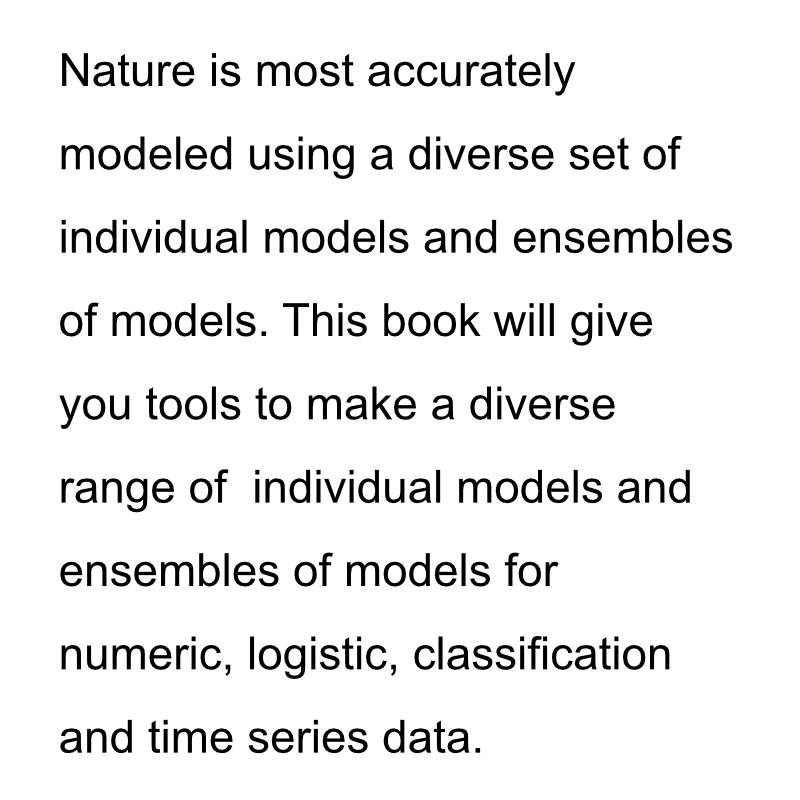
\includegraphics{_book/images/Nature_is_most_accurately_modeled.jpg}
\caption{How nature is most accurately modeled}
\end{figure}

You will be able to do wonderful things as you complete the skills in this book. As the book will show, ensembles are much more accurate than any other method to help us understand and model nature. This will be done with a level of accuracy that has not been achieved previously. And you can do all of it.

The phrase ``wonderful things'' is very intentional. When Howard Carter was doing archaeology, at one point in November, 1922, he was quite sure he found something important. Carter made a small hole to see through. Lord Carnarvon (who was paying for all of this!) asked Howard Carter, ``Can you see anything?. Howard Carter's famous reply,''Yes, wonderful things!{}``. When they opened everything up, they found the intact tomb of Tutankhamun. It contained more than 5,000 items, and enriched our knowledge of ancient Africa beyond any other find.

Here is a tiny taste of one of the more than 5,000 the ``wonderful things'' found by Howard Carter, Lord Carnarvon, and the team of archaeologists.

\begin{figure}
\centering
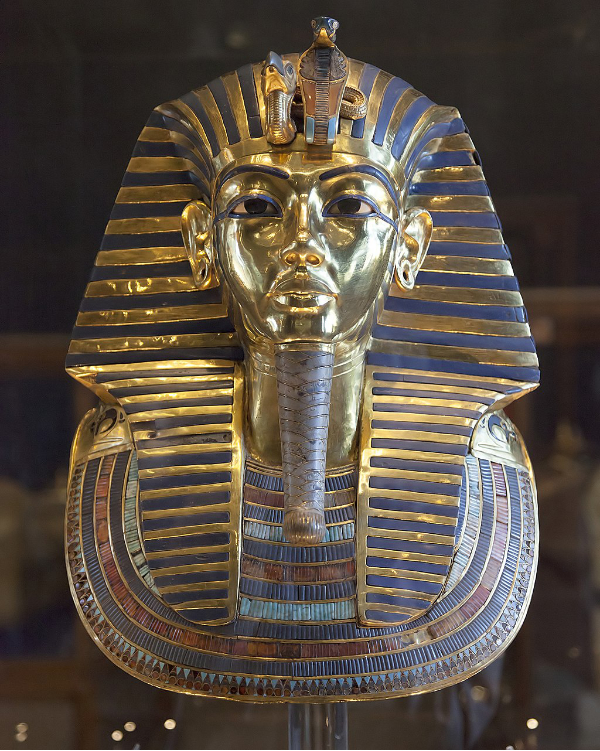
\includegraphics{_book/images/King_Tut_Mask.jpg}
\caption{King Tut Mask}
\end{figure}

I will do my very best to share many ``wonderful things'' through the entire book as you explore the world of ensembles.

The Ensembles package I've made does the entire analysis process for you automatically. This will put the power of ensembles in your hands, give you the strongest foundation for your work, with the highest degree of accuracy.

All of the examples in the book will come from real data. For example (and there are many more examples in the book):

•~HR Analytics

• Predicting the winning time in the London Marathon

• World's most accurate score to a very difficult classification problem

• Beat the best score in student Kaggle competitions

We will have many more practical examples from a very wide range of fields for you to enjoy.

This book will show you how ensembles improve our understanding of nature, and how you can use ensembles in your work. The results using ensembles are much more accurate than has ever been possible before, and that will be demonstrated over and over again in this book. You will be able to use ensembles to understand the world, and build your own models of data, at a level of accuracy that has not been achieved before.

\begin{figure}
\centering
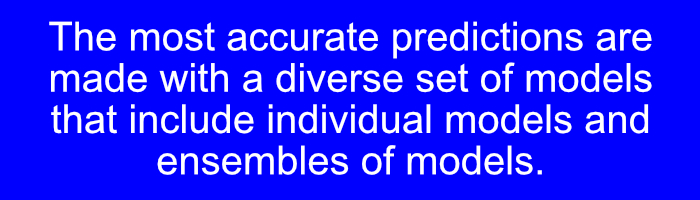
\includegraphics{_book/images/The_most_accurate_predictions.jpg}
\caption{The most accurate predictions}
\end{figure}

\section{Ensembles: The New AI, from beginner to expert}\label{ensembles-the-new-ai-from-beginner-to-expert}

As you will see, Ensembles are the new AI. Science has gone from the calculus of Newton and Leibnetz, to differential equations, to the modern world of creating models, and many points in-between. Ensembles are the most powerful way to put models together to achieve the best possible results. This book will guide you through the process, and show you how you can build ensembles that will pass all testing.

This is the new AI. Welcome to the path, it's extremely fun, and I look forward to sharing it with you!

\section{What you will be able to do by the end of the book}\label{what-you-will-be-able-to-do-by-the-end-of-the-book}

• Make your own customized ensembles of models of numerical, classification, logistic and time series data.

• Use the Ensembles package which does the entire process automatically (but little customization is possible).

• Make your ensemble solutions into packages that can be shared with other users.

• Make your ensemble solutions into totally self-contained solutions that can be shared with anyone.

• Learn how ensembles of models can help to make the wisest possible decision based on the data.

•~Learn how to present the results at different levels, from a regular user to a CEO and board of directors.

• How to present results that are social media friendly.

• Find your own data and create the ensemble solution from beginning to end (called One Of Your Own in the each of the chapter exercises)

• Solve real world examples in this book where ensembles achieve such results as:

• Beat the top score in a student data science competition by over 90\% (numerical ensembles).

• Correctly predict the winning time for the 2024 Men's London Marathon (time series ensembles).

• Produce a 100\% accurate solution to the dry beans classification problem (first in the world with this data set, done using classification ensembles).

• Make recommendations how Lebron James can improve his performance on the basketball court (logistic ensembles).

• Complete a comprehensive Final Project that will put all of your new skills with ensembles together. This result can be shared with employers, advisors, on social media, job interviews, or anywhere else you would like to share your work.

\section{How this book is organized so you learn the material as easily as possible}\label{how-this-book-is-organized-so-you-learn-the-material-as-easily-as-possible}

The book begins with the foundations of making ensembles of models. We will look at:

• Individual numerical models

• Ensembles of numerical models

• Individual classification models

• Ensembles of classification models

• Individual logistic models

• Ensembles of logistic models

• Individual forecasting models

• Ensembles of forecasting models

• Advanced data visualizations

• Multiple ways to communicate your results. This will range from other people in the field, to customers, to the C-Suite (CEO, CTO, board of directors, etc.)

•~We will look at how to treat data science as a business. In particular we will pay close attention to showing return on investment (ROI) in data science, using ensembles of models.

• The book will conclude showing four examples of a final comprehensive project. There will be one example each of numerical data, classification data, logistic data and forecasting data. The example professionally formatted. The source files for each of the eight files are available in a github repository.

\section{How you can learn the skills as fast as possible: How the exercises are organized}\label{how-you-can-learn-the-skills-as-fast-as-possible-how-the-exercises-are-organized}

As a young child, I learned that I have much better retention with a system I have always called delayed repetition. This means that I learn best and fastest when I see a worked out example, do several practice examples, and then repeat that after a delay in time. The delay can range from an hour to a few days.

For example, the exercises in the Individual Classification Models chapter will ask you to build models using techniques from the classification models and the prior chapters. The exercises for logistic ensembles will ask you to build models from the content in the logistic models chapter, and each of the previous chapters. It has been my experience that repeating this over and over is the fastest way for me to learn new content, and retain it for the longest period of time.

By the time you get to the Final Comprehensive Project, your skills will be sharp for each of the modeling techniques.

\section{Going from student to teacher: You are required to post on social media and help others understand the results}\label{going-from-student-to-teacher-you-are-required-to-post-on-social-media-and-help-others-understand-the-results}

One of the most important parts of your role in data science is communicating your findings. I will present many examples of summaries and reports for you to adapt and use on your projects. You are also required to post your results on social media. You may use any appropriate choice of social media, but it needs to be publicly available. This has a number of very important benefits to you:

• You will build a body of work that shows your skill level

• The results will demonstrate your ability to communicate in a way that works with a wide variety of people

• You will work to demonstrate very good skills with video and/or audio production

• Use the hashtag \#AIEnsembles when you post on social media

\section{Helping you use the power of pre-trained ensembles and individual models}\label{helping-you-use-the-power-of-pre-trained-ensembles-and-individual-models}

Another important part of the skills you will learn here includes building pre-trained ensembles and models. The book will walk you through the process of building the pre-trained models and ensembles for each of the four types of data (numerical, classification, logicial, and time series).

\section{Helping you master the material: One of your own exercises}\label{helping-you-master-the-material-one-of-your-own-exercises}

One of the differences with the exercises in Ensembles is the inclusion of One of Your Own exercises. Each set of exercises will include one which asks you to find your own data (with many hints given to help you find data), define the problem, make the ensemble, and report the results.

\begin{figure}
\centering
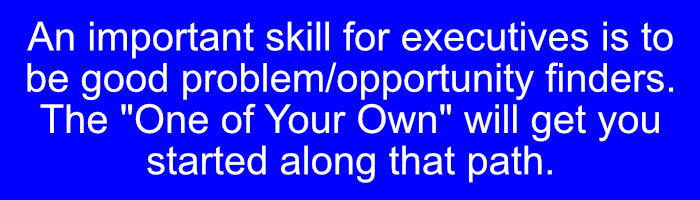
\includegraphics{_book/images/Good_problem_finder.jpg}
\caption{Good problem finder}
\end{figure}

\section{Keeping it real: Actual business data and problems as the source of all the data sets}\label{keeping-it-real-actual-business-data-and-problems-as-the-source-of-all-the-data-sets}

All of the data sets in this book use real data. No exceptions, no synthetic data. The sources of the data are all cited, and the real world implications can be found by a simple search. All of the data is absolutely real.

\section{Check your biases: Test your model on a neutral data set}\label{check-your-biases-test-your-model-on-a-neutral-data-set}

Each set of exercises will ask you to check one of the trained models against a neutral data set. If the model has any biases, this should reveal them. Then you'll have the knowledge to go back and address the biases in the models.

\section{Helping you check your work---and verifying that your results beat previously published results}\label{helping-you-check-your-workand-verifying-that-your-results-beat-previously-published-results}

Many of the data sets have been solved by previous investigators (such as in competitions), so the results here can be easily compared with published results.

For example, we will look at the Boston Housing data set when we look at numerical data sets. This data set has been used many times in Kaggle competitions, published papers, and Github repositories, among many other sources.

The Ensembles package will automatically solve this data set, and return an RMSE less than 0.20 (there will be slight variation depending on how the parameters are set, as will be explained those chapters). In comparison, the Boston Housing data set was used in this Kaggle student competition: \url{https://www.kaggle.com/competitions/uou-g03784-2022-spring/leaderboard?tab=public}, and the best score was 2.09684. The Ensembles package will beat the best result in that Kaggle student competition by more than 90\%. The Ensembles package only requires one line of code.

\section{Helping you work as a team with fully reproducible ensembles and individual models}\label{helping-you-work-as-a-team-with-fully-reproducible-ensembles-and-individual-models}

A large part of the skills you will learn include how to make results that are reproducible. This will include:

• Multiple random resamplings of the data

• Learning how to test on totally unseen data for both individual and ensemble models

• How to repeat results (for example, 25 times), and report the accuracy of each resampling

For example, you will make ensembles of models, and then use those trained models to make predictions on totally unseen data.

\section{The Final Comprehensive Project will put everything together for you}\label{the-final-comprehensive-project-will-put-everything-together-for-you}

As I was studying data science, one of my professors said that the papers I turned in were ``good enough to show to the CEO or Board of Directors'' of the Fortune 1000 company he worked for. The chapter on the Final Comprehensive Project will share the highest level of skills in the following:

• Truly understanding the business problem

• Being able to convey the very high value that data science brings to the table

• Being able to back up 100\% of your claims with rock solid evidence, facts, and clear reasoning

• How to make a truly professional quality presentation worthy of the C-Suite

\begin{figure}
\centering
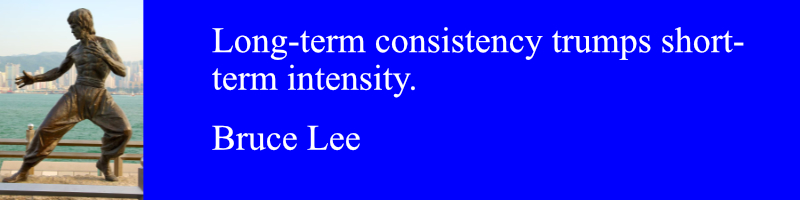
\includegraphics{_book/images/Bruce_Lee.jpg}
\caption{Long term consistency wins the race}
\end{figure}

I've had the incredible pleasure of learning many different skills. A few include being able to play on more than 20 musical instruments, communicate in three languages at a professional level, manage a multi-million dollar division of a Fortune 1000 company, run two non-profit volunteer groups, snowboard a three mile run in Colorado, work as a professional counselor, and much more. The book your reading is only my most recent project. None of these skills were acquired overnight. A huge part of the success is being able to make slow and (usually) steady progress. The next chapter will reveal the big secret to getting results, but for now you are best off if you plan some regular time to work on the contents of the book.

Always remember to test everything, that will save you a ton of problems down the road.

\section{Exercises to help improve your skills}\label{exercises-to-help-improve-your-skills}

Exercise 1: Schedule regular time to work on this book

You will gain much more progress if you work at a steady pace. Take everything in small pieces. It's OK to go slow, as long as you keep going. Schedule regular time to work on this book, and you will get the largest possible reward for your efforts.

Exercise 2: Read each chapter at least twice \textbf{before} you begin working on the material.

Reading each chapter twice before you begin working on it will actually speed up your progress and results. It will actually take less time for you to complete the chapter. You might not believe it right now, but it's totally true.

Exercise 2a: Read a chapter ahead if you are able to do so.

Exercise 3: Read this chapter again

\chapter{Introduction and your first ensembles}\label{introduction-and-your-first-ensembles}

\section{How a Chicago blizzard led to the very unlikely story of the best solutions to supervised data}\label{how-a-chicago-blizzard-led-to-the-very-unlikely-story-of-the-best-solutions-to-supervised-data}

My journey to the most advanced AI in the world started with an actual
blizzard in Chicago. It might seem like Chicago would never get a
blizzard, but we did in 2011, and it was incredibly intense, as this
video shows:

\url{https://www.youtube.com/watch?v=cPiFn52ztd8}

What does the \href{https://en.wikipedia.org/wiki/2011_Groundhog_Day_blizzard}{Chicago 2011
Snomageddon}
have to do with the creation of the most advanced AI? Everything. Here's
the story.

At the time of the 2011 Blizzard I worked a Recruiter for \href{https://en.wikipedia.org/wiki/Kelly_Services}{Kelly
Services}, where I had
worked since 1996. I agreed to work out of the Kelly Services office in
Frankfort, Illinois at this time, though I worked out of nearly every
Kelly Services office at one time or another. The trip to Frankfort
involved a daily commute to the office, but I was able to make the best
use of the time on the road.

My manager at the time let me know several days in advance that there
was a very large amount of snow forecast, and that I might want to be
prepared. The most recent forecasts for large amounts of snow in the
Chicago area all amounted to nothing. They were perfectly normal days in
the Chicago area, so I predicted this storm would also be nothing, based
on the most recent results. This was a great example of a prior
prediction not transferring well to a current situation.

That morning I went to work as normal, and did not even look at the
weather forecast. Around 2:45 pm my manager came out of her office and
said ``Russ, you need to come here and look at the weather radar!''. I
walked into her office, and saw a map of a winter storm that was
incredibly huge. She had the image zoomed out, so it was possible to see
several states. From what I could tell, the massive snow storm was
barreling down on Chicago, and was about 15 minutes away from our
location.

I told the candidate I was interviewing that I was leaving immediately,
and that he is not allowed to stay. He has to get home as fast as
possible for his own safety.

The storm started dropping snow on my trip north back home. The commute
took around 50\% longer than normal due to the rapidly falling snow.

As I later learned, the storm was forecast to start in the Chicago area
around 3:00 pm, finish up between 11:00 am - 1:00 pm two days later, and
leave 17 - 19 inches of snow.

How bad was it? Even City of Chicago snow plows were stopped by the
snow:

\begin{figure}
\centering
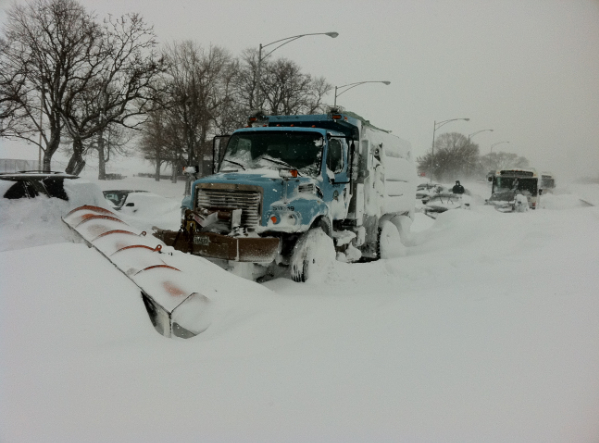
\includegraphics{_book/images/Chicago_Snow_Plow_stuck_on_Lake_Shore_drive_Chicago_Feb_2_2011_storm.jpg}
\caption{\href{https://en.wikipedia.org/wiki/2011_Groundhog_Day_blizzard\#/media/File:Stuck_Salt_Truck_on_Lake_Shore_drive_Chicago_Feb_2_2011_storm.JPG}{Chicago snow
plow}
stuck on Lake Shore Drive in the 2011 snow
storm}
\end{figure}

To see what the forecasts looked like, check out this news report from
the day:

\url{https://www.nbcchicago.com/news/local/blizzard-unleashes-winter-fury/2096753/}

It turns out all three predictions of the blizzard were accurate to a
level that almost seemed uncanny to me: Start time, accumulation, and
end time were all spot on. This is the first time I recall ever seeing a
prediction at this level of accuracy. I had no idea this type of
predictive accuracy was even possible. This level of accuracy in
predicting results totally blew me away. I had never seen anything with
this level of accuracy, and now I wanted to know how it was done.

I searched and searched for how the accuracy was so high for this
forecast.

The power of the method---whatever it was---was obvious to me. I realized
that if it could work for the weather, the solution method could work in
an incredibly broad range of situations. A few of many other areas
include business forecasts, production work, modeling prices, and much,
much more. But that this point I had no idea how the accurate prediction
was done.

Some months later a person wrote to \href{https://en.wikipedia.org/wiki/Tom_Skilling}{Tom
Skilling}, chief
meteorologist for WGN TV in Chicago. Tom posted an answer that opened up
the solution for me. Here is the relevant part of \href{https://www.facebook.com/TomSkilling/posts/531146448370303}{Tom Skilling's
answer} to a
2011 storm how the forecast was so accurate:

\begin{quote}
The Weather Service has developed an interesting ``SNOWFALL ENSEMBLE
FORECAST PROBABILITY SYSTEM'' which draws upon a wide range of snow
accumulation forecasts from a whole set of different computer models.
By ``blending'' these model projections, probability of snowfalls
falling within certain ranges becomes possible. Also, this ``blending''
of multiple forecasts ``smooths'' the sometimes huge model disparities
in the amounts being predicted. The resulting probabilities therefore
represent a ``best case'' forecast.
\end{quote}

So that was the first step. Ensembles were the way they achieved such
extraordinary prediction accuracy.

My next goal was to figure out how ensembles were made. As I looked up
information, it became obvious that ensembles had been used for a while,
such as the winning entry in the Netflix Prize Competition:

\begin{figure}
\centering
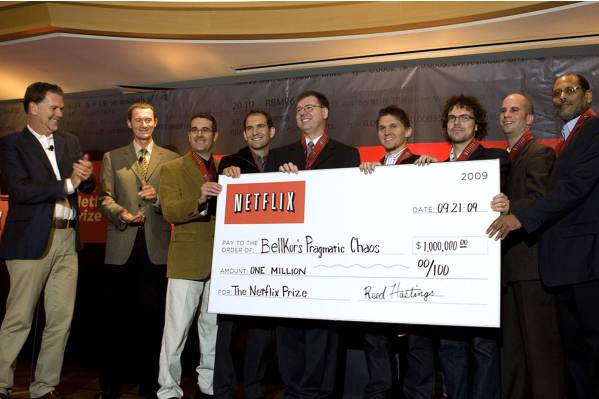
\includegraphics{_book/images/netflix_prize.jpg}
\caption{Netflix Prize Competition}
\end{figure}

The \href{https://en.wikipedia.org/wiki/Netflix_Prize}{Netflix Prize
Competition} was sponsored
by Netflix to create a method to accurately predict user ratings on
films. The minimum winning score needed to beat the Netflix method
(named Cinematch) by at least 10\%. Several years of work went into
solving this problem, and the results even included several published
papers. The winning solution was an ensemble of methods that beat the
Cinematch results by 10.09\%.

So it was now clear to me that ensembles were the path forward. However,
I had no idea how to make ensembles.

I went to graduate school to study data science and predictive
analytics. My degree was completed in 2017, from Northwestern
University. However, I still was not sure how ensembles of models were
built, nor could I find any clear methods to build them (except for
pre-made methods, such as random forests). While it is true there were
packages that could do some of the work, nothing I found did what I was
looking for: How to build ensembles of models in general. Despite
playing with the idea and looking online, I was not able to build the
ensembles I wanted to build.

\section{Saturday, October 15, 2022 at 4:58 pm. The exact birth of the Ensembles system}\label{saturday-october-15-2022-at-458-pm.-the-exact-birth-of-the-ensembles-system}

Everything changed on Saturday, October 15, 2022 at 4:58 pm. I was
playing with various methods to make an ensemble, and got an ensemble
that worked for the very first time. While the results were extremely
modest by any standards, it was clear to me that the foundation was
there to build a general solution that can work in an extremely wide
range of areas. Here is my journal entry:

\begin{figure}
\centering
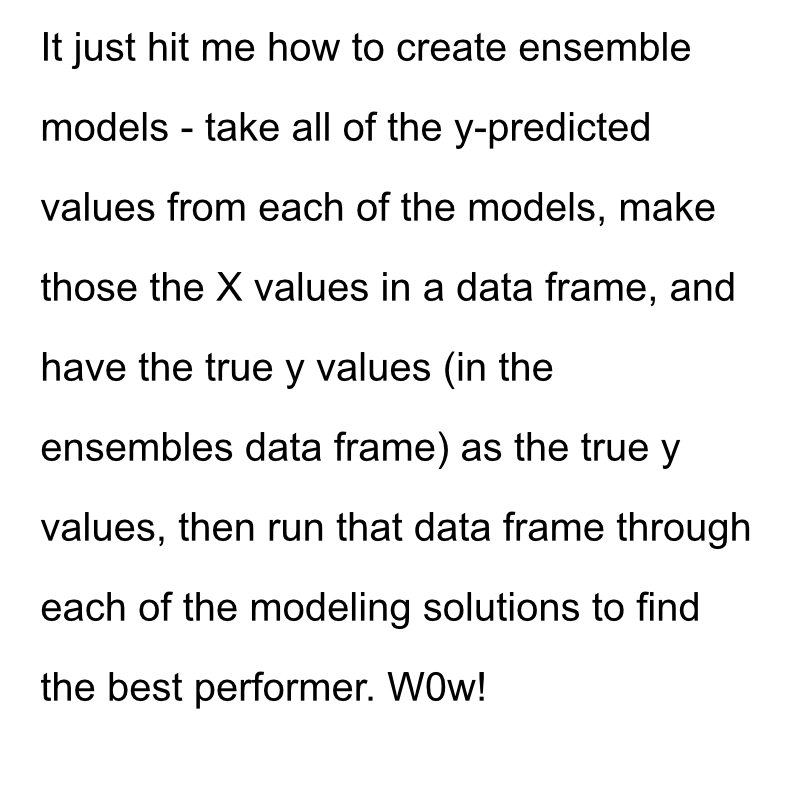
\includegraphics{_book/images/Birth_of_ensembles.jpg}
\caption{Birth of the ensembles method (typo of W0w in the
original)}
\end{figure}

You might be asking yourself how I know the day and time. That is a very
reasonable question. I've been keeping a journal since I was 19 years
old, and have thousands of entries. As soon as I realized how to
correctly build ensembles, I made this entry, which contains the key
elements to make an ensemble, and we will do these steps in just a
moment. Notice that the subject line in the journal matches the text
above.

One of the ways to improve your skills is to keep a journal, and we'll
be looking at that in more depth in this chapter and future chapters.
The journal I use is \href{https://danschimpf.com/}{MacJournal}, though there
are a large number of other options available on the market.

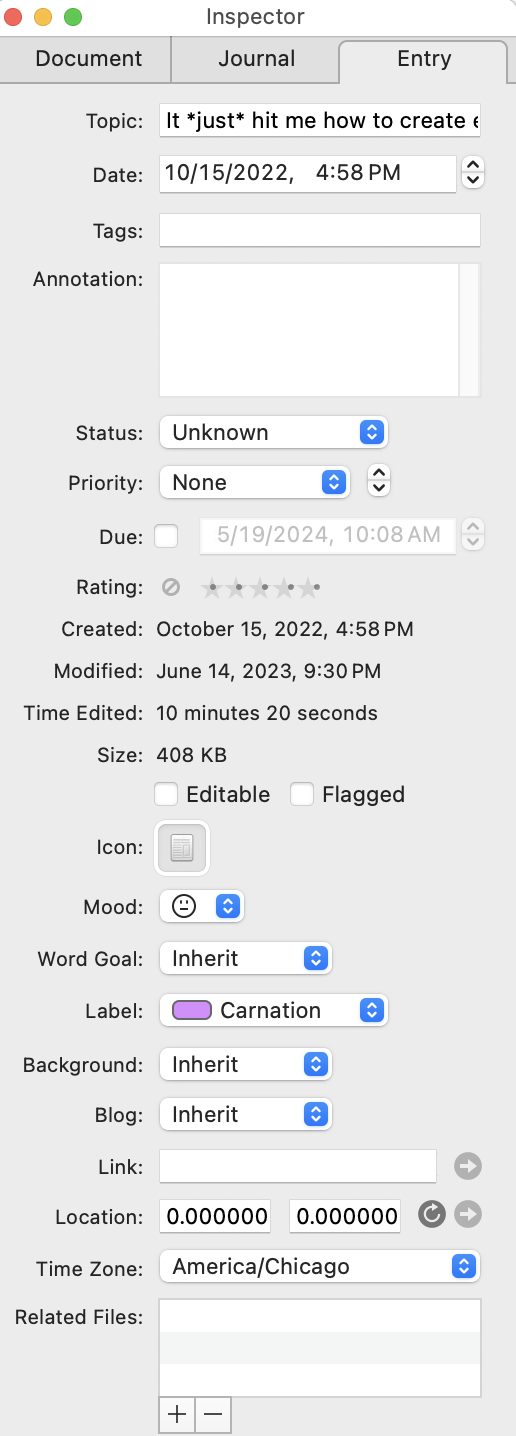
\includegraphics{_book/images/Journal_birth_of_ensembles.png}

Birth of ensembles, Saturday, October 15, 2022 at 4:58 pm

\begin{figure}
\centering

\includegraphics{_book/images/Keep_a_journal.jpg}
\caption{Keep a journal}
\end{figure}

\section{Here is what an ensemble of models looks like at the most basic level, using the Boston Housing data set as an example:}\label{here-is-what-an-ensemble-of-models-looks-like-at-the-most-basic-level-using-the-boston-housing-data-set-as-an-example}

\subsection{Head of Boston Housing data set}\label{head-of-boston-housing-data-set}

\begin{figure}
\centering
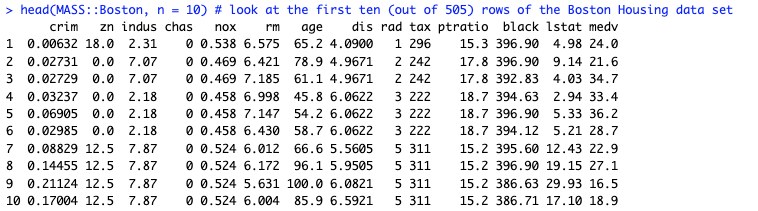
\includegraphics{_book/images/Boston_Housing_data_head.png}
\caption{Head of Boston Housing data
set}
\end{figure}

We will start our first ensemble with a data set that only has numerical
values. Our first example will use the Boston Housing data set, from the
MASS package. While the Boston Housing data set is controversial (and we
will discuss some of the controversies in our example making
professional quality reports for the C-Suite), for now it works as a
very well known data set to begin our journey into ensembles.

Overview of the most basic steps to make an ensemble:

We will be using the Boston Housing data set, so let's have a look at
some Boston images:

\begin{figure}
\centering
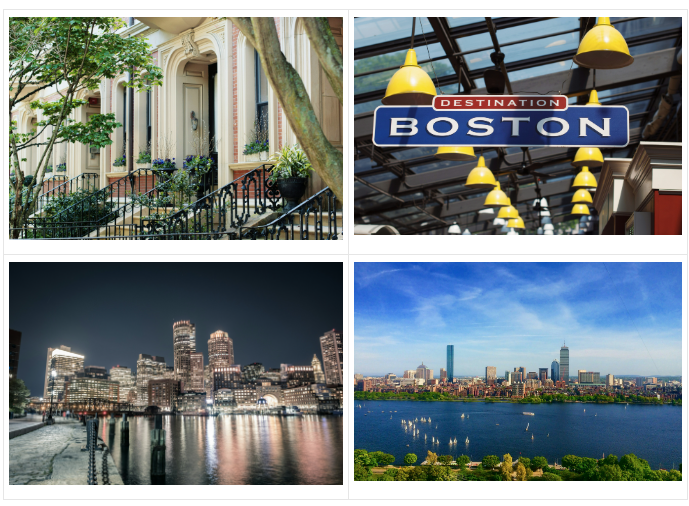
\includegraphics{_book/images/Boston.png}
\caption{Boston}
\end{figure}

\section{The steps to build your first ensemble from scratch}\label{the-steps-to-build-your-first-ensemble-from-scratch}

\begin{itemize}
\item
  Load the packages we will need (MASS, tree)
\item
  Load the Boston Housing data set, and split it into train (60\%) and
  test (40\%) sections.
\item
  Create a linear model by fitting the linear model on the training
  data, and make predictions on the Boston Housing test data. Measure
  the accuracy of the predictions against the actual values.
\item
  Create a model using trees by fitting the tree model on the training
  data, and making predictions on the Boston Housing test data.
  Measure the accuracy of the predictions against the actual values.
\item
  Make a new data frame. This will be our ensemble of model
  predictions. One column will be the linear predictions, and one will
  be the tree predictions.
\item
  Make a new column for the true values---these are the true values in
  the Boston Housing test data set
\item
  Once we have the new ensemble data set, it's simply another data
  set. No different in many ways from any other data set (except how
  it was made).
\item
  Break the ensemble data set into train (60\%) and test (40\%)
  sections.
\item
  Fit a linear model to the ensemble training data. Make predictions
  using the testing data, and measure the accuracy of the predictions
  against the test data.
\item
  Summarize the results.
\end{itemize}

\textbf{I suggest reading the over of the most basic steps to make an ensemble
a couple of times, to make sure you are very familiar with the steps.}

\section{Building the first actual ensemble}\label{building-the-first-actual-ensemble}

Load the packages we will need (MASS, tree):

\begin{Shaded}
\begin{Highlighting}[]
\FunctionTok{library}\NormalTok{(MASS) }\CommentTok{\# for the Boston Housing data set}
\FunctionTok{library}\NormalTok{(tree) }\CommentTok{\# To make models using trees}
\FunctionTok{library}\NormalTok{(Metrics) }\CommentTok{\# To calculate error rate (root mean squared error)}
\FunctionTok{library}\NormalTok{(tidyverse)}
\CommentTok{\#\textgreater{} {-}{-} Attaching core tidyverse packages {-}{-}{-}{-} tidyverse 2.0.0 {-}{-}}
\CommentTok{\#\textgreater{} v dplyr     1.1.4     v readr     2.1.5}
\CommentTok{\#\textgreater{} v forcats   1.0.0     v stringr   1.5.1}
\CommentTok{\#\textgreater{} v ggplot2   3.5.1     v tibble    3.2.1}
\CommentTok{\#\textgreater{} v lubridate 1.9.3     v tidyr     1.3.1}
\CommentTok{\#\textgreater{} v purrr     1.0.2     }
\CommentTok{\#\textgreater{} {-}{-} Conflicts {-}{-}{-}{-}{-}{-}{-}{-}{-}{-}{-}{-}{-}{-}{-}{-}{-}{-}{-}{-}{-}{-} tidyverse\_conflicts() {-}{-}}
\CommentTok{\#\textgreater{} x dplyr::filter() masks stats::filter()}
\CommentTok{\#\textgreater{} x dplyr::lag()    masks stats::lag()}
\CommentTok{\#\textgreater{} x dplyr::select() masks MASS::select()}
\CommentTok{\#\textgreater{} i Use the conflicted package (\textless{}http://conflicted.r{-}lib.org/\textgreater{}) to force all conflicts to become errors}
\end{Highlighting}
\end{Shaded}

Load the Boston Housing data set, and split it into train (60\%) and test
(40\%) sections.

\begin{Shaded}
\begin{Highlighting}[]
\NormalTok{df }\OtherTok{\textless{}{-}}\NormalTok{ MASS}\SpecialCharTok{::}\NormalTok{Boston}
\NormalTok{train }\OtherTok{\textless{}{-}}\NormalTok{ df[}\DecValTok{1}\SpecialCharTok{:}\DecValTok{400}\NormalTok{, ]}
\NormalTok{test }\OtherTok{\textless{}{-}}\NormalTok{ df[}\DecValTok{401}\SpecialCharTok{:}\DecValTok{505}\NormalTok{, ]}

\CommentTok{\# Let\textquotesingle{}s have a quick look at the train and test sets}
\FunctionTok{head}\NormalTok{(train)}
\CommentTok{\#\textgreater{}      crim zn indus chas   nox    rm  age    dis rad tax}
\CommentTok{\#\textgreater{} 1 0.00632 18  2.31    0 0.538 6.575 65.2 4.0900   1 296}
\CommentTok{\#\textgreater{} 2 0.02731  0  7.07    0 0.469 6.421 78.9 4.9671   2 242}
\CommentTok{\#\textgreater{} 3 0.02729  0  7.07    0 0.469 7.185 61.1 4.9671   2 242}
\CommentTok{\#\textgreater{} 4 0.03237  0  2.18    0 0.458 6.998 45.8 6.0622   3 222}
\CommentTok{\#\textgreater{} 5 0.06905  0  2.18    0 0.458 7.147 54.2 6.0622   3 222}
\CommentTok{\#\textgreater{} 6 0.02985  0  2.18    0 0.458 6.430 58.7 6.0622   3 222}
\CommentTok{\#\textgreater{}   ptratio  black lstat medv}
\CommentTok{\#\textgreater{} 1    15.3 396.90  4.98 24.0}
\CommentTok{\#\textgreater{} 2    17.8 396.90  9.14 21.6}
\CommentTok{\#\textgreater{} 3    17.8 392.83  4.03 34.7}
\CommentTok{\#\textgreater{} 4    18.7 394.63  2.94 33.4}
\CommentTok{\#\textgreater{} 5    18.7 396.90  5.33 36.2}
\CommentTok{\#\textgreater{} 6    18.7 394.12  5.21 28.7}
\FunctionTok{head}\NormalTok{(test)}
\CommentTok{\#\textgreater{}         crim zn indus chas   nox    rm   age    dis rad tax}
\CommentTok{\#\textgreater{} 401 25.04610  0  18.1    0 0.693 5.987 100.0 1.5888  24 666}
\CommentTok{\#\textgreater{} 402 14.23620  0  18.1    0 0.693 6.343 100.0 1.5741  24 666}
\CommentTok{\#\textgreater{} 403  9.59571  0  18.1    0 0.693 6.404 100.0 1.6390  24 666}
\CommentTok{\#\textgreater{} 404 24.80170  0  18.1    0 0.693 5.349  96.0 1.7028  24 666}
\CommentTok{\#\textgreater{} 405 41.52920  0  18.1    0 0.693 5.531  85.4 1.6074  24 666}
\CommentTok{\#\textgreater{} 406 67.92080  0  18.1    0 0.693 5.683 100.0 1.4254  24 666}
\CommentTok{\#\textgreater{}     ptratio  black lstat medv}
\CommentTok{\#\textgreater{} 401    20.2 396.90 26.77  5.6}
\CommentTok{\#\textgreater{} 402    20.2 396.90 20.32  7.2}
\CommentTok{\#\textgreater{} 403    20.2 376.11 20.31 12.1}
\CommentTok{\#\textgreater{} 404    20.2 396.90 19.77  8.3}
\CommentTok{\#\textgreater{} 405    20.2 329.46 27.38  8.5}
\CommentTok{\#\textgreater{} 406    20.2 384.97 22.98  5.0}
\end{Highlighting}
\end{Shaded}

Create a linear model by fitting the linear model on the training data,
and make predictions on the Boston Housing test data. Measure the
accuracy of the predictions against the actual values.

\begin{Shaded}
\begin{Highlighting}[]
\NormalTok{Boston\_lm }\OtherTok{\textless{}{-}} \FunctionTok{lm}\NormalTok{(medv }\SpecialCharTok{\textasciitilde{}}\NormalTok{ ., }\AttributeTok{data =}\NormalTok{ train) }\CommentTok{\# Fit the model to the training data}
\NormalTok{Boston\_lm\_predictions }\OtherTok{\textless{}{-}} \FunctionTok{predict}\NormalTok{(}\AttributeTok{object =}\NormalTok{ Boston\_lm, }\AttributeTok{newdata =}\NormalTok{ test)}

\CommentTok{\# Let\textquotesingle{}s have a quick look at the model predictions}
\FunctionTok{head}\NormalTok{(Boston\_lm\_predictions)}
\CommentTok{\#\textgreater{}       401       402       403       404       405       406 }
\CommentTok{\#\textgreater{} 12.618507 19.785728 20.919370 13.014507  6.946392  5.123039}
\end{Highlighting}
\end{Shaded}

Calculate the error for the model

\begin{Shaded}
\begin{Highlighting}[]
\NormalTok{Boston\_linear\_RMSE }\OtherTok{\textless{}{-}}\NormalTok{ Metrics}\SpecialCharTok{::}\FunctionTok{rmse}\NormalTok{(}\AttributeTok{actual =}\NormalTok{ test}\SpecialCharTok{$}\NormalTok{medv, }\AttributeTok{predicted =}\NormalTok{ Boston\_lm\_predictions)}
\NormalTok{Boston\_linear\_RMSE}
\CommentTok{\#\textgreater{} [1] 6.108005}
\end{Highlighting}
\end{Shaded}

The error rate for the linear model is 6.108005. Let's do the same using
the tree method.

Create a model using trees by fitting the tree model on the training
data, and making predictions on the Boston Housing test data. Measure
the accuracy of the predictions against the actual values.

\begin{Shaded}
\begin{Highlighting}[]
\NormalTok{Boston\_tree }\OtherTok{\textless{}{-}} \FunctionTok{tree}\NormalTok{(medv }\SpecialCharTok{\textasciitilde{}}\NormalTok{ ., }\AttributeTok{data =}\NormalTok{ train) }\CommentTok{\# Fit the model to the training data}
\NormalTok{Boston\_tree\_predictions }\OtherTok{\textless{}{-}} \FunctionTok{predict}\NormalTok{(}\AttributeTok{object =}\NormalTok{ Boston\_tree, }\AttributeTok{newdata =}\NormalTok{ test)}

\CommentTok{\# Let\textquotesingle{}s have a quick look at the predictions:}
\FunctionTok{head}\NormalTok{(Boston\_tree\_predictions)}
\CommentTok{\#\textgreater{}      401      402      403      404      405      406 }
\CommentTok{\#\textgreater{} 13.30769 13.30769 13.30769 13.30769 13.30769 13.30769}
\end{Highlighting}
\end{Shaded}

Calculate the error rate for the tree model:

\begin{Shaded}
\begin{Highlighting}[]
\NormalTok{Boston\_tree\_RMSE }\OtherTok{\textless{}{-}}\NormalTok{ Metrics}\SpecialCharTok{::}\FunctionTok{rmse}\NormalTok{(}\AttributeTok{actual =}\NormalTok{ test}\SpecialCharTok{$}\NormalTok{medv, }\AttributeTok{predicted =}\NormalTok{ Boston\_tree\_predictions)}
\NormalTok{Boston\_tree\_RMSE}
\CommentTok{\#\textgreater{} [1] 5.478017}
\end{Highlighting}
\end{Shaded}

The error rate for the tree model is lower (which is better). The error
rate for the tree model is 5.478017.

\section{We're ready to make our first ensemble!!}\label{were-ready-to-make-our-first-ensemble}

Make a new data frame. This will be our ensemble of model predictions,
and one column for the true values. One column will be the linear
predictions, and one will be the tree predictions. We'll make a third
column, the true values.

Make a new column for the true values---these are the true values in the
Boston Housing test data set

\begin{Shaded}
\begin{Highlighting}[]
\NormalTok{ensemble }\OtherTok{\textless{}{-}} \FunctionTok{data.frame}\NormalTok{(}
  \StringTok{\textquotesingle{}linear\textquotesingle{}} \OtherTok{=}\NormalTok{ Boston\_lm\_predictions,}
  \StringTok{\textquotesingle{}tree\textquotesingle{}} \OtherTok{=}\NormalTok{ Boston\_tree\_predictions,}
  \StringTok{\textquotesingle{}y\textquotesingle{}} \OtherTok{=}\NormalTok{ test}\SpecialCharTok{$}\NormalTok{medv}
\NormalTok{)}

\CommentTok{\# Let\textquotesingle{}s have a look at the ensemble:}
\FunctionTok{head}\NormalTok{(ensemble)}
\CommentTok{\#\textgreater{}        linear     tree    y}
\CommentTok{\#\textgreater{} 401 12.618507 13.30769  5.6}
\CommentTok{\#\textgreater{} 402 19.785728 13.30769  7.2}
\CommentTok{\#\textgreater{} 403 20.919370 13.30769 12.1}
\CommentTok{\#\textgreater{} 404 13.014507 13.30769  8.3}
\CommentTok{\#\textgreater{} 405  6.946392 13.30769  8.5}
\CommentTok{\#\textgreater{} 406  5.123039 13.30769  5.0}
\FunctionTok{dim}\NormalTok{(ensemble)}
\CommentTok{\#\textgreater{} [1] 105   3}
\end{Highlighting}
\end{Shaded}

Once we have the new ensemble data set, it's simply another data set. No
different in many ways from any other data set (except how it was made).

Break the ensemble data set into train (60\%) and test (40\%) sections.
There is nothing special about the 60/40 split here, you may use any
numbers you wish.

\begin{Shaded}
\begin{Highlighting}[]
\NormalTok{ensemble\_train }\OtherTok{\textless{}{-}}\NormalTok{ ensemble[}\DecValTok{1}\SpecialCharTok{:}\DecValTok{60}\NormalTok{, ]}
\NormalTok{ensemble\_test }\OtherTok{\textless{}{-}}\NormalTok{ ensemble[}\DecValTok{61}\SpecialCharTok{:}\DecValTok{105}\NormalTok{, ]}

\FunctionTok{head}\NormalTok{(ensemble\_train)}
\CommentTok{\#\textgreater{}        linear     tree    y}
\CommentTok{\#\textgreater{} 401 12.618507 13.30769  5.6}
\CommentTok{\#\textgreater{} 402 19.785728 13.30769  7.2}
\CommentTok{\#\textgreater{} 403 20.919370 13.30769 12.1}
\CommentTok{\#\textgreater{} 404 13.014507 13.30769  8.3}
\CommentTok{\#\textgreater{} 405  6.946392 13.30769  8.5}
\CommentTok{\#\textgreater{} 406  5.123039 13.30769  5.0}
\FunctionTok{head}\NormalTok{(ensemble\_test)}
\CommentTok{\#\textgreater{}       linear     tree    y}
\CommentTok{\#\textgreater{} 461 23.88984 13.30769 16.4}
\CommentTok{\#\textgreater{} 462 23.29129 13.30769 17.7}
\CommentTok{\#\textgreater{} 463 22.54055 21.84327 19.5}
\CommentTok{\#\textgreater{} 464 25.50940 21.84327 20.2}
\CommentTok{\#\textgreater{} 465 22.71231 21.84327 21.4}
\CommentTok{\#\textgreater{} 466 20.83810 21.84327 19.9}
\end{Highlighting}
\end{Shaded}

Fit a linear model to the ensemble training data. Make predictions using
the testing data, and measure the accuracy of the predictions against
the test data. Notice how similar this is to our linear and tree models.

\begin{Shaded}
\begin{Highlighting}[]
\CommentTok{\# Fit the model to the training data}
\NormalTok{ensemble\_lm }\OtherTok{\textless{}{-}} \FunctionTok{lm}\NormalTok{(y }\SpecialCharTok{\textasciitilde{}}\NormalTok{ ., }\AttributeTok{data =}\NormalTok{ ensemble\_train)}

\CommentTok{\# Make predictions using the model on the test data}
\NormalTok{ensemble\_lm\_predictions }\OtherTok{\textless{}{-}} \FunctionTok{predict}\NormalTok{(}\AttributeTok{object =}\NormalTok{ ensemble\_lm, }\AttributeTok{newdata =}\NormalTok{ ensemble\_test)}

\CommentTok{\# Calculate error rate for the ensemble predictions}
\NormalTok{ensemble\_lm\_rmse }\OtherTok{\textless{}{-}}\NormalTok{ Metrics}\SpecialCharTok{::}\FunctionTok{rmse}\NormalTok{(}\AttributeTok{actual =}\NormalTok{ ensemble\_test}\SpecialCharTok{$}\NormalTok{y, }\AttributeTok{predicted =}\NormalTok{ ensemble\_lm\_predictions)}

\CommentTok{\# Report the error rate for the ensemble}
\NormalTok{ensemble\_lm\_rmse}
\CommentTok{\#\textgreater{} [1] 4.826962}
\end{Highlighting}
\end{Shaded}

Summarize the results.

\begin{Shaded}
\begin{Highlighting}[]
\NormalTok{results }\OtherTok{\textless{}{-}} \FunctionTok{data.frame}\NormalTok{(}
  \StringTok{\textquotesingle{}Model\textquotesingle{}} \OtherTok{=} \FunctionTok{c}\NormalTok{(}\StringTok{\textquotesingle{}Linear\textquotesingle{}}\NormalTok{, }\StringTok{\textquotesingle{}Tree\textquotesingle{}}\NormalTok{, }\StringTok{\textquotesingle{}Ensemble\textquotesingle{}}\NormalTok{),}
  \StringTok{\textquotesingle{}Error\textquotesingle{}} \OtherTok{=} \FunctionTok{c}\NormalTok{(Boston\_linear\_RMSE, Boston\_tree\_RMSE, ensemble\_lm\_rmse)}
\NormalTok{)}

\NormalTok{results}
\CommentTok{\#\textgreater{}      Model    Error}
\CommentTok{\#\textgreater{} 1   Linear 6.108005}
\CommentTok{\#\textgreater{} 2     Tree 5.478017}
\CommentTok{\#\textgreater{} 3 Ensemble 4.826962}
\end{Highlighting}
\end{Shaded}

Clearly the ensemble had the lowest error rate of the three models. The
ensemble is easily the best of the three models because it has the
lowest error rate of all the models.

\subsection{Try it yourself: Make an ensemble where the ensemble is made using trees instead of linear models.}\label{try-it-yourself-make-an-ensemble-where-the-ensemble-is-made-using-trees-instead-of-linear-models.}

\begin{Shaded}
\begin{Highlighting}[]
\CommentTok{\# Fit the model to the training data}
\NormalTok{ensemble\_tree }\OtherTok{\textless{}{-}} \FunctionTok{tree}\NormalTok{(y }\SpecialCharTok{\textasciitilde{}}\NormalTok{ ., }\AttributeTok{data =}\NormalTok{ ensemble\_train)}

\CommentTok{\# Make predictions using the model on the test data}
\NormalTok{ensemble\_tree\_predict }\OtherTok{\textless{}{-}} \FunctionTok{predict}\NormalTok{(}\AttributeTok{object =}\NormalTok{ ensemble\_tree, }\AttributeTok{newdata =}\NormalTok{ ensemble\_test)}

\CommentTok{\# Let\textquotesingle{}s look at the predictions}
\FunctionTok{head}\NormalTok{(ensemble\_tree\_predict)}
\CommentTok{\#\textgreater{}      461      462      463      464      465      466 }
\CommentTok{\#\textgreater{} 14.80000 14.80000 18.94286 18.94286 18.94286 18.94286}

\CommentTok{\# Calculate the error rate}
\NormalTok{ensemble\_tree\_rmse }\OtherTok{\textless{}{-}}\NormalTok{ Metrics}\SpecialCharTok{::}\FunctionTok{rmse}\NormalTok{(}\AttributeTok{actual =}\NormalTok{ ensemble\_test}\SpecialCharTok{$}\NormalTok{y, }\AttributeTok{predicted =}\NormalTok{ ensemble\_tree\_predict)}

\NormalTok{ensemble\_tree\_rmse}
\CommentTok{\#\textgreater{} [1] 5.322011}
\end{Highlighting}
\end{Shaded}

How does this compare to our three other results? Let's update the
results table

\begin{Shaded}
\begin{Highlighting}[]
\NormalTok{results }\OtherTok{\textless{}{-}} \FunctionTok{data.frame}\NormalTok{(}
  \StringTok{\textquotesingle{}Model\textquotesingle{}} \OtherTok{=} \FunctionTok{c}\NormalTok{(}\StringTok{\textquotesingle{}Linear\textquotesingle{}}\NormalTok{, }\StringTok{\textquotesingle{}Tree\textquotesingle{}}\NormalTok{, }\StringTok{\textquotesingle{}Ensemble\_Linear\textquotesingle{}}\NormalTok{, }\StringTok{\textquotesingle{}Ensemble\_Tree\textquotesingle{}}\NormalTok{),}
  \StringTok{\textquotesingle{}Error\textquotesingle{}} \OtherTok{=} \FunctionTok{c}\NormalTok{(Boston\_linear\_RMSE, Boston\_tree\_RMSE, ensemble\_lm\_rmse, ensemble\_tree\_rmse)}
\NormalTok{)}

\NormalTok{results }\OtherTok{\textless{}{-}}\NormalTok{ results }\SpecialCharTok{\%\textgreater{}\%} \FunctionTok{arrange}\NormalTok{(Error)}

\NormalTok{results}
\CommentTok{\#\textgreater{}             Model    Error}
\CommentTok{\#\textgreater{} 1 Ensemble\_Linear 4.826962}
\CommentTok{\#\textgreater{} 2   Ensemble\_Tree 5.322011}
\CommentTok{\#\textgreater{} 3            Tree 5.478017}
\CommentTok{\#\textgreater{} 4          Linear 6.108005}
\end{Highlighting}
\end{Shaded}

\subsection{Both of the ensemble models beat both of the individual models in this example}\label{both-of-the-ensemble-models-beat-both-of-the-individual-models-in-this-example}

\section{Principle: What is one improvement that can be made? Use a diverse set of models and ensembles to get the best possible result}\label{principle-what-is-one-improvement-that-can-be-made-use-a-diverse-set-of-models-and-ensembles-to-get-the-best-possible-result}

As we shall see when we go through and learn how to build ensembles, the
numerical method we will use will build 27 individual models and 13
ensembles for a total of 40 results. When the goal is to get the best
possible results, a diverse set of models and ensembles, such as the 40
results for numerical data, will produce much better results than a
limited number of models and ensembles.

We will do the same principal when we are looking at classification
data, logistic, data, and time series forecasting data. We will use a
large number of individual models and ensembles with the goal of
achieving the best possible result.

\section{Principle: Randomizing the data before the analysis will make the results more general (and is very easy to do!)}\label{principle-randomizing-the-data-before-the-analysis-will-make-the-results-more-general-and-is-very-easy-to-do}

\begin{Shaded}
\begin{Highlighting}[]
\NormalTok{df }\OtherTok{\textless{}{-}}\NormalTok{ df[}\FunctionTok{sample}\NormalTok{(}\FunctionTok{nrow}\NormalTok{(df)),] }\CommentTok{\# Randomize the rows before the analysis}
\end{Highlighting}
\end{Shaded}

\section{Try it yourself: Repeat the previous analysis, but randomize the rows before the analysis. Otherwise keep the process the same. Share your results on social media.}\label{try-it-yourself-repeat-the-previous-analysis-but-randomize-the-rows-before-the-analysis.-otherwise-keep-the-process-the-same.-share-your-results-on-social-media.}

We'll follow the exact same steps, except for randomizing the rows
first.

• Randomize the rows

• Break the data into train and test sets

•~Fit the model to the training set

•~Make predictions and calculate error from the model on the test set

\begin{Shaded}
\begin{Highlighting}[]
\NormalTok{df }\OtherTok{\textless{}{-}}\NormalTok{ df[}\FunctionTok{sample}\NormalTok{(}\FunctionTok{nrow}\NormalTok{(df)),] }\CommentTok{\# Randomize the rows before the analysis}

\NormalTok{train }\OtherTok{\textless{}{-}}\NormalTok{ df[}\DecValTok{1}\SpecialCharTok{:}\DecValTok{400}\NormalTok{, ]}
\NormalTok{test }\OtherTok{\textless{}{-}}\NormalTok{ df[}\DecValTok{401}\SpecialCharTok{:}\DecValTok{505}\NormalTok{, ]}

\CommentTok{\# Fit the model to the training data}
\NormalTok{Boston\_lm }\OtherTok{\textless{}{-}} \FunctionTok{lm}\NormalTok{(medv }\SpecialCharTok{\textasciitilde{}}\NormalTok{ ., }\AttributeTok{data =}\NormalTok{ train)}

\CommentTok{\# Make predictions using the model on the test data}
\NormalTok{Boston\_lm\_predictions }\OtherTok{\textless{}{-}} \FunctionTok{predict}\NormalTok{(}\AttributeTok{object =}\NormalTok{ Boston\_lm, }\AttributeTok{newdata =}\NormalTok{ test)}

\CommentTok{\# Let\textquotesingle{}s have a quick look at the linear model predictions:}

\FunctionTok{head}\NormalTok{(Boston\_lm\_predictions)}
\CommentTok{\#\textgreater{}      191      382      128       18       30      484 }
\CommentTok{\#\textgreater{} 30.84277 17.99259 15.32377 16.70613 20.60622 20.58334}
\end{Highlighting}
\end{Shaded}

\begin{Shaded}
\begin{Highlighting}[]
\NormalTok{Boston\_linear\_rmse }\OtherTok{\textless{}{-}}\NormalTok{ Metrics}\SpecialCharTok{::}\FunctionTok{rmse}\NormalTok{(}\AttributeTok{actual =}\NormalTok{ test}\SpecialCharTok{$}\NormalTok{medv, }\AttributeTok{predicted =}\NormalTok{ Boston\_lm\_predictions)}

\NormalTok{Boston\_tree }\OtherTok{\textless{}{-}} \FunctionTok{tree}\NormalTok{(medv }\SpecialCharTok{\textasciitilde{}}\NormalTok{ ., }\AttributeTok{data =}\NormalTok{ train)}
\NormalTok{Boston\_tree\_predictions }\OtherTok{\textless{}{-}} \FunctionTok{predict}\NormalTok{(}\AttributeTok{object =}\NormalTok{ Boston\_tree, }\AttributeTok{newdata =}\NormalTok{ test)}
\NormalTok{Boston\_tree\_rmse }\OtherTok{\textless{}{-}}\NormalTok{ Metrics}\SpecialCharTok{::}\FunctionTok{rmse}\NormalTok{(}\AttributeTok{actual =}\NormalTok{ test}\SpecialCharTok{$}\NormalTok{medv, }\AttributeTok{predicted =}\NormalTok{ Boston\_tree\_predictions)}

\CommentTok{\# Let\textquotesingle{}s have a quick look at the tree model predictions:}

\FunctionTok{head}\NormalTok{(Boston\_tree\_predictions)}
\CommentTok{\#\textgreater{}      191      382      128       18       30      484 }
\CommentTok{\#\textgreater{} 24.26522 11.60615 17.25875 17.25875 20.91807 20.91807}
\end{Highlighting}
\end{Shaded}

\begin{Shaded}
\begin{Highlighting}[]
\NormalTok{ensemble }\OtherTok{\textless{}{-}} \FunctionTok{data.frame}\NormalTok{( }\StringTok{\textquotesingle{}linear\textquotesingle{}} \OtherTok{=}\NormalTok{ Boston\_lm\_predictions, }\StringTok{\textquotesingle{}tree\textquotesingle{}} \OtherTok{=}\NormalTok{ Boston\_tree\_predictions, }\StringTok{\textquotesingle{}y\_ensemble\textquotesingle{}} \OtherTok{=}\NormalTok{ test}\SpecialCharTok{$}\NormalTok{medv )}

\NormalTok{ensemble }\OtherTok{\textless{}{-}}\NormalTok{ ensemble[}\FunctionTok{sample}\NormalTok{(}\FunctionTok{nrow}\NormalTok{(ensemble)), ] }\CommentTok{\# Randomizes the rows of the ensemble}

\NormalTok{ensemble\_train }\OtherTok{\textless{}{-}}\NormalTok{ ensemble[}\DecValTok{1}\SpecialCharTok{:}\DecValTok{60}\NormalTok{, ]}
\NormalTok{ensemble\_test }\OtherTok{\textless{}{-}}\NormalTok{ ensemble[}\DecValTok{61}\SpecialCharTok{:}\DecValTok{105}\NormalTok{, ]}
\end{Highlighting}
\end{Shaded}

\begin{Shaded}
\begin{Highlighting}[]
\NormalTok{ensemble\_lm }\OtherTok{\textless{}{-}} \FunctionTok{lm}\NormalTok{(y\_ensemble }\SpecialCharTok{\textasciitilde{}}\NormalTok{ ., }\AttributeTok{data =}\NormalTok{ ensemble\_train)}

\CommentTok{\# Predictions for the ensemble linear model}

\NormalTok{ensemble\_prediction }\OtherTok{\textless{}{-}} \FunctionTok{predict}\NormalTok{(ensemble\_lm, }\AttributeTok{newdata =}\NormalTok{ ensemble\_test)}

\CommentTok{\# Root mean squared error for the ensemble linear model}

\NormalTok{ensemble\_lm\_rmse }\OtherTok{\textless{}{-}}\NormalTok{ Metrics}\SpecialCharTok{::}\FunctionTok{rmse}\NormalTok{(}\AttributeTok{actual =}\NormalTok{ ensemble\_test}\SpecialCharTok{$}\NormalTok{y\_ensemble, }\AttributeTok{predicted =}\NormalTok{ ensemble\_prediction)}

\CommentTok{\# Same for tree models}

\NormalTok{ensemble\_tree }\OtherTok{\textless{}{-}} \FunctionTok{tree}\NormalTok{(y\_ensemble }\SpecialCharTok{\textasciitilde{}}\NormalTok{ ., }\AttributeTok{data =}\NormalTok{ ensemble\_train)}
\NormalTok{ensemble\_tree\_predictions }\OtherTok{\textless{}{-}} \FunctionTok{predict}\NormalTok{(}\AttributeTok{object =}\NormalTok{ ensemble\_tree, }\AttributeTok{newdata =}\NormalTok{ ensemble\_test)}
\NormalTok{ensemble\_tree\_rmse }\OtherTok{\textless{}{-}}\NormalTok{ Metrics}\SpecialCharTok{::}\FunctionTok{rmse}\NormalTok{(}\AttributeTok{actual =}\NormalTok{ ensemble\_test}\SpecialCharTok{$}\NormalTok{y\_ensemble, }\AttributeTok{predicted =}\NormalTok{ ensemble\_tree\_predictions)}

\NormalTok{results }\OtherTok{\textless{}{-}} \FunctionTok{list}\NormalTok{( }\StringTok{\textquotesingle{}Linear\textquotesingle{}} \OtherTok{=}\NormalTok{ Boston\_linear\_rmse, }\StringTok{\textquotesingle{}Trees\textquotesingle{}} \OtherTok{=}\NormalTok{ Boston\_tree\_rmse, }\StringTok{\textquotesingle{}Ensembles\_Linear\textquotesingle{}} \OtherTok{=}\NormalTok{ ensemble\_lm\_rmse, }\StringTok{\textquotesingle{}Ensemble\_Tree\textquotesingle{}} \OtherTok{=}\NormalTok{ ensemble\_tree\_rmse )}

\NormalTok{results}
\CommentTok{\#\textgreater{} $Linear}
\CommentTok{\#\textgreater{} [1] 4.606489}
\CommentTok{\#\textgreater{} }
\CommentTok{\#\textgreater{} $Trees}
\CommentTok{\#\textgreater{} [1] 4.384072}
\CommentTok{\#\textgreater{} }
\CommentTok{\#\textgreater{} $Ensembles\_Linear}
\CommentTok{\#\textgreater{} [1] 3.489345}
\CommentTok{\#\textgreater{} }
\CommentTok{\#\textgreater{} $Ensemble\_Tree}
\CommentTok{\#\textgreater{} [1] 5.33012}
\end{Highlighting}
\end{Shaded}

The fact that our results are a bit different from our first ensemble is
useful. This gives us another solid principle to use in our analysis
methods:

\section{The more we can randomize the data, the more our results will match nature}\label{the-more-we-can-randomize-the-data-the-more-our-results-will-match-nature}

Just watch: Repeat the results 100 times, return the mean of the results
(hint: It's two small changes)

\begin{Shaded}
\begin{Highlighting}[]
\ControlFlowTok{for}\NormalTok{ (i }\ControlFlowTok{in} \DecValTok{1}\SpecialCharTok{:}\DecValTok{100}\NormalTok{) \{}

\CommentTok{\# First the linear model with randomized data}

\NormalTok{df }\OtherTok{\textless{}{-}}\NormalTok{ df[}\FunctionTok{sample}\NormalTok{(}\FunctionTok{nrow}\NormalTok{(df)),] }\CommentTok{\# Randomize the rows before the analysis}

\NormalTok{train }\OtherTok{\textless{}{-}}\NormalTok{ df[}\DecValTok{1}\SpecialCharTok{:}\DecValTok{400}\NormalTok{, ]}
\NormalTok{test }\OtherTok{\textless{}{-}}\NormalTok{ df[}\DecValTok{401}\SpecialCharTok{:}\DecValTok{505}\NormalTok{, ]}

\NormalTok{Boston\_lm }\OtherTok{\textless{}{-}} \FunctionTok{lm}\NormalTok{(medv }\SpecialCharTok{\textasciitilde{}}\NormalTok{ ., }\AttributeTok{data =}\NormalTok{ train)}
\NormalTok{Boston\_lm\_predictions }\OtherTok{\textless{}{-}} \FunctionTok{predict}\NormalTok{(}\AttributeTok{object =}\NormalTok{ Boston\_lm, }\AttributeTok{newdata =}\NormalTok{ test)}

\CommentTok{\# Let\textquotesingle{}s have a quick look at the linear model predictions:}

\FunctionTok{head}\NormalTok{(Boston\_lm\_predictions)}

\CommentTok{\# Let\textquotesingle{}s calculate the root mean squared error rate of the predictions:}

\NormalTok{Boston\_linear\_rmse[i] }\OtherTok{\textless{}{-}}\NormalTok{ Metrics}\SpecialCharTok{::}\FunctionTok{rmse}\NormalTok{(}\AttributeTok{actual =}\NormalTok{ test}\SpecialCharTok{$}\NormalTok{medv, }\AttributeTok{predicted =}\NormalTok{ Boston\_lm\_predictions)}

\NormalTok{Boston\_linear\_rmse\_mean }\OtherTok{\textless{}{-}} \FunctionTok{mean}\NormalTok{(Boston\_linear\_rmse)}

\CommentTok{\# Let\textquotesingle{}s use tree models}

\NormalTok{Boston\_tree }\OtherTok{\textless{}{-}} \FunctionTok{tree}\NormalTok{(medv }\SpecialCharTok{\textasciitilde{}}\NormalTok{ ., }\AttributeTok{data =}\NormalTok{ train)}

\NormalTok{Boston\_tree\_predictions }\OtherTok{\textless{}{-}} \FunctionTok{predict}\NormalTok{(}\AttributeTok{object =}\NormalTok{ Boston\_tree, }\AttributeTok{newdata =}\NormalTok{ test)}

\CommentTok{\# Let\textquotesingle{}s have a quick look at the tree model predictions:}

\FunctionTok{head}\NormalTok{(Boston\_tree\_predictions)}

\CommentTok{\# Let\textquotesingle{}s calculate the root mean squared error rate of the predictions:}

\NormalTok{Boston\_tree\_rmse[i] }\OtherTok{\textless{}{-}}\NormalTok{ Metrics}\SpecialCharTok{::}\FunctionTok{rmse}\NormalTok{(}\AttributeTok{actual =}\NormalTok{ test}\SpecialCharTok{$}\NormalTok{medv, }\AttributeTok{predicted =}\NormalTok{ Boston\_tree\_predictions) }
\NormalTok{Boston\_tree\_rmse\_mean }\OtherTok{\textless{}{-}} \FunctionTok{mean}\NormalTok{(Boston\_tree\_rmse)}

\NormalTok{ensemble }\OtherTok{\textless{}{-}} \FunctionTok{data.frame}\NormalTok{(}\StringTok{\textquotesingle{}linear\textquotesingle{}} \OtherTok{=}\NormalTok{ Boston\_lm\_predictions, }\StringTok{\textquotesingle{}tree\textquotesingle{}} \OtherTok{=}\NormalTok{ Boston\_tree\_predictions, }\StringTok{\textquotesingle{}y\_ensemble\textquotesingle{}} \OtherTok{=}\NormalTok{ test}\SpecialCharTok{$}\NormalTok{medv )}

\NormalTok{ensemble }\OtherTok{\textless{}{-}}\NormalTok{ ensemble[}\FunctionTok{sample}\NormalTok{(}\FunctionTok{nrow}\NormalTok{(ensemble)), ] }\CommentTok{\# Randomizes the rows of the ensemble}

\NormalTok{ensemble\_train }\OtherTok{\textless{}{-}}\NormalTok{ ensemble[}\DecValTok{1}\SpecialCharTok{:}\DecValTok{60}\NormalTok{, ]}
\NormalTok{ensemble\_test }\OtherTok{\textless{}{-}}\NormalTok{ ensemble[}\DecValTok{61}\SpecialCharTok{:}\DecValTok{105}\NormalTok{, ]}

\CommentTok{\# Ensemble linear modeling}

\NormalTok{ensemble\_lm }\OtherTok{\textless{}{-}} \FunctionTok{lm}\NormalTok{(y\_ensemble }\SpecialCharTok{\textasciitilde{}}\NormalTok{ ., }\AttributeTok{data =}\NormalTok{ ensemble\_train)}

\CommentTok{\# Predictions for the ensemble linear model}

\NormalTok{ensemble\_prediction }\OtherTok{\textless{}{-}} \FunctionTok{predict}\NormalTok{(ensemble\_lm, }\AttributeTok{newdata =}\NormalTok{ ensemble\_test)}

\CommentTok{\# Root mean squared error for the ensemble linear model}

\NormalTok{ensemble\_lm\_rmse[i] }\OtherTok{\textless{}{-}}\NormalTok{ Metrics}\SpecialCharTok{::}\FunctionTok{rmse}\NormalTok{(}\AttributeTok{actual =}\NormalTok{ ensemble\_test}\SpecialCharTok{$}\NormalTok{y\_ensemble, }\AttributeTok{predicted =}\NormalTok{ ensemble\_prediction)}

\NormalTok{ensemble\_lm\_rmse\_mean }\OtherTok{\textless{}{-}} \FunctionTok{mean}\NormalTok{(ensemble\_lm\_rmse)}

\NormalTok{ensemble\_tree }\OtherTok{\textless{}{-}} \FunctionTok{tree}\NormalTok{(y\_ensemble }\SpecialCharTok{\textasciitilde{}}\NormalTok{ ., }\AttributeTok{data =}\NormalTok{ ensemble\_train)}

\NormalTok{ensemble\_tree\_predictions }\OtherTok{\textless{}{-}} \FunctionTok{predict}\NormalTok{(}\AttributeTok{object =}\NormalTok{ ensemble\_tree, }\AttributeTok{newdata =}\NormalTok{ ensemble\_test) }

\NormalTok{ensemble\_tree\_rmse[i] }\OtherTok{\textless{}{-}}\NormalTok{ Metrics}\SpecialCharTok{::}\FunctionTok{rmse}\NormalTok{(}\AttributeTok{actual =}\NormalTok{ ensemble\_test}\SpecialCharTok{$}\NormalTok{y\_ensemble, }\AttributeTok{predicted =} 
\NormalTok{ensemble\_tree\_predictions)}

\NormalTok{ensemble\_tree\_rmse\_mean }\OtherTok{\textless{}{-}} \FunctionTok{mean}\NormalTok{(ensemble\_tree\_rmse)}

\NormalTok{results }\OtherTok{\textless{}{-}} \FunctionTok{data.frame}\NormalTok{(}
  \StringTok{\textquotesingle{}Linear\textquotesingle{}} \OtherTok{=}\NormalTok{ Boston\_linear\_rmse\_mean,}
  \StringTok{\textquotesingle{}Trees\textquotesingle{}} \OtherTok{=}\NormalTok{ Boston\_tree\_rmse\_mean,}
  \StringTok{\textquotesingle{}Ensembles\_Linear\textquotesingle{}} \OtherTok{=}\NormalTok{ ensemble\_lm\_rmse\_mean,}
  \StringTok{\textquotesingle{}Ensemble\_Tree\textquotesingle{}} \OtherTok{=}\NormalTok{ ensemble\_tree\_rmse\_mean )}

\NormalTok{\}}

\NormalTok{results}
\CommentTok{\#\textgreater{}     Linear    Trees Ensembles\_Linear Ensemble\_Tree}
\CommentTok{\#\textgreater{} 1 4.825244 4.573845         4.186623      5.134664}
\FunctionTok{warnings}\NormalTok{() }\CommentTok{\# No warnings!}
\end{Highlighting}
\end{Shaded}

\begin{figure}
\centering
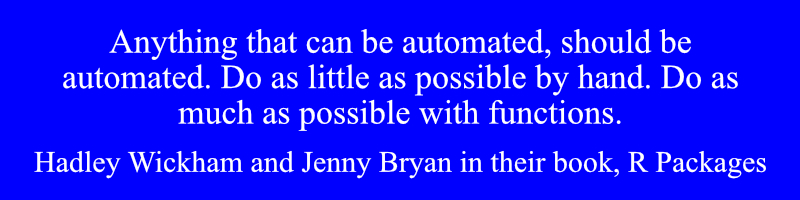
\includegraphics{_book/images/automate_as_much_as_possible.jpg}
\caption{Automate as much as
possible}
\end{figure}

\section{Principle: ``Is this my very best work?''}\label{principle-is-this-my-very-best-work}

This is your best work to build ensembles at this stage of your skills.
We are going to make a number of improvements to the solutions we see
here, so our final result will be much stronger than what we have here
so far. Always strive to do your very best work, without any excuses.

\section{``Where do I get help with errors or warnings?''}\label{where-do-i-get-help-with-errors-or-warnings}

It is extremely useful to check if your code returns any errors or
warnings, and fix those as fast as possible. There are numerous sites to
help address errors in your code:

\url{https://stackoverflow.com}

\url{https://forum.posit.co}

\url{https://www.r-project.org/help.html}

\section{Is there an easy way to save all trained models?}\label{is-there-an-easy-way-to-save-all-trained-models}

Absolutely! We will simply add the code at the end of this section that
saves the four trained models (linear, tree, ensemble\_linear and
ensemble\_tree), as follows:

\begin{Shaded}
\begin{Highlighting}[]
\FunctionTok{library}\NormalTok{(MASS)}
\FunctionTok{library}\NormalTok{(Metrics)}
\FunctionTok{library}\NormalTok{(tree)}

\NormalTok{ensemble\_lm\_rmse }\OtherTok{\textless{}{-}} \DecValTok{0}
\NormalTok{ensemble\_tree\_rmse }\OtherTok{\textless{}{-}} \DecValTok{0}

\ControlFlowTok{for}\NormalTok{ (i }\ControlFlowTok{in} \DecValTok{1}\SpecialCharTok{:}\DecValTok{100}\NormalTok{) \{}

\CommentTok{\# Fit the linear model with randomized data}

\NormalTok{df }\OtherTok{\textless{}{-}}\NormalTok{ df[}\FunctionTok{sample}\NormalTok{(}\FunctionTok{nrow}\NormalTok{(df)),] }\CommentTok{\# Randomize the rows before the analysis}

\NormalTok{train }\OtherTok{\textless{}{-}}\NormalTok{ df[}\DecValTok{1}\SpecialCharTok{:}\DecValTok{400}\NormalTok{, ]}
\NormalTok{test }\OtherTok{\textless{}{-}}\NormalTok{ df[}\DecValTok{401}\SpecialCharTok{:}\DecValTok{505}\NormalTok{, ]}

\NormalTok{Boston\_lm }\OtherTok{\textless{}{-}} \FunctionTok{lm}\NormalTok{(medv }\SpecialCharTok{\textasciitilde{}}\NormalTok{ ., }\AttributeTok{data =}\NormalTok{ train)}

\NormalTok{Boston\_lm\_predictions }\OtherTok{\textless{}{-}} \FunctionTok{predict}\NormalTok{(}\AttributeTok{object =}\NormalTok{ Boston\_lm, }\AttributeTok{newdata =}\NormalTok{ test)}

\CommentTok{\# Let\textquotesingle{}s have a quick look at the linear model predictions:}

\FunctionTok{head}\NormalTok{(Boston\_lm\_predictions)}

\CommentTok{\# Let\textquotesingle{}s calculate the root mean squared error rate of the predictions:}

\NormalTok{Boston\_linear\_rmse[i] }\OtherTok{\textless{}{-}}\NormalTok{ Metrics}\SpecialCharTok{::}\FunctionTok{rmse}\NormalTok{(}\AttributeTok{actual =}\NormalTok{ test}\SpecialCharTok{$}\NormalTok{medv, }\AttributeTok{predicted =}\NormalTok{ Boston\_lm\_predictions) }
\NormalTok{Boston\_linear\_rmse\_mean }\OtherTok{\textless{}{-}} \FunctionTok{mean}\NormalTok{(Boston\_linear\_rmse)}

\CommentTok{\# Let\textquotesingle{}s use tree models}

\NormalTok{Boston\_tree }\OtherTok{\textless{}{-}} \FunctionTok{tree}\NormalTok{(medv }\SpecialCharTok{\textasciitilde{}}\NormalTok{ ., }\AttributeTok{data =}\NormalTok{ train)}

\NormalTok{Boston\_tree\_predictions }\OtherTok{\textless{}{-}} \FunctionTok{predict}\NormalTok{(}\AttributeTok{object =}\NormalTok{ Boston\_tree, }\AttributeTok{newdata =}\NormalTok{ test)}

\CommentTok{\# Let\textquotesingle{}s have a quick look at the tree model predictions:}

\FunctionTok{head}\NormalTok{(Boston\_tree\_predictions)}

\CommentTok{\# Let\textquotesingle{}s calculate the root mean squared error rate of the predictions:}

\NormalTok{Boston\_tree\_rmse[i] }\OtherTok{\textless{}{-}}\NormalTok{ Metrics}\SpecialCharTok{::}\FunctionTok{rmse}\NormalTok{(}\AttributeTok{actual =}\NormalTok{ test}\SpecialCharTok{$}\NormalTok{medv, }\AttributeTok{predicted =}\NormalTok{ Boston\_tree\_predictions) }
\NormalTok{Boston\_tree\_rmse\_mean }\OtherTok{\textless{}{-}} \FunctionTok{mean}\NormalTok{(Boston\_tree\_rmse)}

\NormalTok{ensemble }\OtherTok{\textless{}{-}} \FunctionTok{data.frame}\NormalTok{( }\StringTok{\textquotesingle{}linear\textquotesingle{}} \OtherTok{=}\NormalTok{ Boston\_lm\_predictions, }\StringTok{\textquotesingle{}tree\textquotesingle{}} \OtherTok{=}\NormalTok{ Boston\_tree\_predictions, }\StringTok{\textquotesingle{}y\_ensemble\textquotesingle{}} \OtherTok{=}\NormalTok{ test}\SpecialCharTok{$}\NormalTok{medv )}

\NormalTok{ensemble }\OtherTok{\textless{}{-}}\NormalTok{ ensemble[}\FunctionTok{sample}\NormalTok{(}\FunctionTok{nrow}\NormalTok{(ensemble)), ] }\CommentTok{\# Randomizes the rows of the ensemble}

\NormalTok{ensemble\_train }\OtherTok{\textless{}{-}}\NormalTok{ ensemble[}\DecValTok{1}\SpecialCharTok{:}\DecValTok{60}\NormalTok{, ]}

\NormalTok{ensemble\_test }\OtherTok{\textless{}{-}}\NormalTok{ ensemble[}\DecValTok{61}\SpecialCharTok{:}\DecValTok{105}\NormalTok{, ]}

\CommentTok{\# Ensemble linear modeling}

\NormalTok{ensemble\_lm }\OtherTok{\textless{}{-}} \FunctionTok{lm}\NormalTok{(y\_ensemble }\SpecialCharTok{\textasciitilde{}}\NormalTok{ ., }\AttributeTok{data =}\NormalTok{ ensemble\_train)}

\CommentTok{\# Predictions for the ensemble linear model}

\NormalTok{ensemble\_prediction }\OtherTok{\textless{}{-}} \FunctionTok{predict}\NormalTok{(ensemble\_lm, }\AttributeTok{newdata =}\NormalTok{ ensemble\_test)}

\CommentTok{\# Root mean squared error for the ensemble linear model}

\NormalTok{ensemble\_lm\_rmse[i] }\OtherTok{\textless{}{-}}\NormalTok{ Metrics}\SpecialCharTok{::}\FunctionTok{rmse}\NormalTok{(}\AttributeTok{actual =}\NormalTok{ ensemble\_test}\SpecialCharTok{$}\NormalTok{y\_ensemble, }\AttributeTok{predicted =}\NormalTok{ ensemble\_prediction)}

\NormalTok{ensemble\_lm\_rmse\_mean }\OtherTok{\textless{}{-}} \FunctionTok{mean}\NormalTok{(ensemble\_lm\_rmse)}

\NormalTok{ensemble\_tree }\OtherTok{\textless{}{-}} \FunctionTok{tree}\NormalTok{(y\_ensemble }\SpecialCharTok{\textasciitilde{}}\NormalTok{ ., }\AttributeTok{data =}\NormalTok{ ensemble\_train)}

\NormalTok{ensemble\_tree\_predictions }\OtherTok{\textless{}{-}} \FunctionTok{predict}\NormalTok{(}\AttributeTok{object =}\NormalTok{ ensemble\_tree, }\AttributeTok{newdata =}\NormalTok{ ensemble\_test) }

\NormalTok{ensemble\_tree\_rmse[i] }\OtherTok{\textless{}{-}}\NormalTok{ Metrics}\SpecialCharTok{::}\FunctionTok{rmse}\NormalTok{(}\AttributeTok{actual =}\NormalTok{ ensemble\_test}\SpecialCharTok{$}\NormalTok{y\_ensemble, }\AttributeTok{predicted =}\NormalTok{ ensemble\_tree\_predictions)}

\NormalTok{ensemble\_tree\_rmse\_mean }\OtherTok{\textless{}{-}} \FunctionTok{mean}\NormalTok{(ensemble\_tree\_rmse)}

\NormalTok{results }\OtherTok{\textless{}{-}} \FunctionTok{list}\NormalTok{( }\StringTok{\textquotesingle{}Linear\textquotesingle{}} \OtherTok{=}\NormalTok{ Boston\_linear\_rmse\_mean, }\StringTok{\textquotesingle{}Trees\textquotesingle{}} \OtherTok{=}\NormalTok{ Boston\_tree\_rmse\_mean, }\StringTok{\textquotesingle{}Ensembles\_Linear\textquotesingle{}} \OtherTok{=}\NormalTok{ ensemble\_lm\_rmse\_mean, }\StringTok{\textquotesingle{}Ensemble\_Tree\textquotesingle{}} \OtherTok{=}\NormalTok{ ensemble\_tree\_rmse\_mean )}

\NormalTok{\}}

\NormalTok{results}
\CommentTok{\#\textgreater{} $Linear}
\CommentTok{\#\textgreater{} [1] 4.969499}
\CommentTok{\#\textgreater{} }
\CommentTok{\#\textgreater{} $Trees}
\CommentTok{\#\textgreater{} [1] 4.812232}
\CommentTok{\#\textgreater{} }
\CommentTok{\#\textgreater{} $Ensembles\_Linear}
\CommentTok{\#\textgreater{} [1] 4.328306}
\CommentTok{\#\textgreater{} }
\CommentTok{\#\textgreater{} $Ensemble\_Tree}
\CommentTok{\#\textgreater{} [1] 5.281115}
\FunctionTok{warnings}\NormalTok{()}
\end{Highlighting}
\end{Shaded}

\begin{Shaded}
\begin{Highlighting}[]

\NormalTok{Boston\_lm }\OtherTok{\textless{}{-}}\NormalTok{ Boston\_lm}
\NormalTok{Boston\_tree }\OtherTok{\textless{}{-}}\NormalTok{ Boston\_tree}
\NormalTok{ensemble\_lm }\OtherTok{\textless{}{-}}\NormalTok{ ensemble\_lm}
\NormalTok{ensemble\_tree }\OtherTok{\textless{}{-}}\NormalTok{ ensemble\_tree}
\end{Highlighting}
\end{Shaded}

\subsection{What about classification, logistic and time series data?}\label{what-about-classification-logistic-and-time-series-data}

In subsequent chapters we will do similar processes with classification,
logistic and time series data. It's possible to build ensembles with all
these types of data. The results are extremely similar to the results
we've seen here with numerical data: While the ensembles won't always
have the best results, it is best to have a diverse set of models and
ensembles to get the best possible results.

\subsection{Principle: Ensembles can work with many types of data, and we will do that in this book}\label{principle-ensembles-can-work-with-many-types-of-data-and-we-will-do-that-in-this-book}

\subsection{Can it make predictions on totally new data from the trained models---including the ensembles?}\label{can-it-make-predictions-on-totally-new-data-from-the-trained-modelsincluding-the-ensembles}

The solutions in this book are independent of the use of the data. We
will look at everything from housing prices to business analysis to HR
analytics to research in medicine. One of our later examples will do
exactly what this question is asking---build individual and ensemble
models from data, then use those pre-trained models to make predictions
on totally unseen data. You will develop this set of skills later in the
book, but it's a minor extension of what you're already seen and
completed.

\subsection{The way I was taught how to write code was totally wrong for me: The best way for me is to start at the end and work backward from there. Do not start coding looking for a solution, instead, start with the ending and work backwards from there.}\label{the-way-i-was-taught-how-to-write-code-was-totally-wrong-for-me-the-best-way-for-me-is-to-start-at-the-end-and-work-backward-from-there.-do-not-start-coding-looking-for-a-solution-instead-start-with-the-ending-and-work-backwards-from-there.}

\begin{figure}
\centering
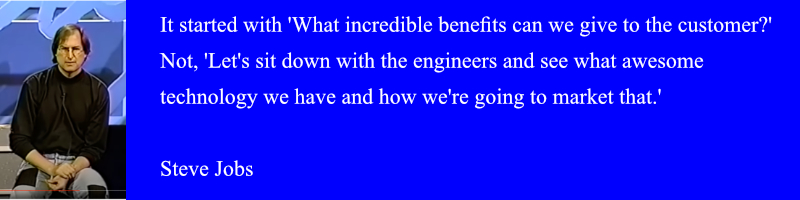
\includegraphics{_book/images/Steve Jobs.jpg}
\caption{Start at the end and work backwards}
\end{figure}

\href{https://www.youtube.com/watch?v=oeqPrUmVz-o}{Start at the end and work backwards from
there}

The biggest lesson for me in all of this work is how to make ensembles.
You've already seen some of the steps, and there are more results to
come. The second biggest lesson is that everything I was taught about
how to do data science and AI was backwards to what actually works for
me in real life. I've learned how I learn, and applied that skill
(learning how I learn) to a wide range of skills, including:

•~Running a multi-million dollar division of a Fortune 1000 company,
including full profit and loss responsibility

• Performing at a professional level on many musical instruments

•~Able to communicate in English, Spanish and sign language in a
professional setting

•~Earning the \#1 place on the annual undergradate university mathematics
competition---twice

• Completing a Master's degree in Guidance and Counseling, allowing me
to help many people in their path toward a healthier life

• Leader of the Oak Park, Illinois chapter of Amnesty International for
ten years, helping to release several Prisoners of Conscience

• President of the Chicago Apple User Group for ten years, helping many
people do extremely good work with their hardware and software

•~Leg press 1,000 pounds ten times in a row

•~Climbed a mountain in Colorado

• Completed multiple skydives (and looking forward to doing more)

The point here is that I have learned how I learn, and I've applied that
skill to many areas. When I started learning data science/AI/coding, it
was all very different from the way I was being creative my whole life.
The way that works for me is to start at the end, work backward from
there, and never give up. Maybe the best evidence of the success of this
method is this fact:

\textbf{When I started to write the code that led to the Ensembles package, I
followed those steps: Start at the end, work backward from there, and
never give up. I wound up writing an average of 1,000 lines of clean,
error free code per month for 15 months. The Ensembles package is around
15,000 lines of clean, error free code.}

I found my attitude was much more important than my skill set, by a long
shot.

\subsection{How I stuck with it all the way to the end: The best career advice I ever received was from a homeless man I never met, and answers the question of what most strongly predicts success.}\label{how-i-stuck-with-it-all-the-way-to-the-end-the-best-career-advice-i-ever-received-was-from-a-homeless-man-i-never-met-and-answers-the-question-of-what-most-strongly-predicts-success.}

\begin{figure}
\centering

\includegraphics{_book/images/Ashford_and_Simpson.png}
\caption{Ashford and Simpson}
\end{figure}

Ashford and Simpson

Learning about building ensembles will help you make more accurate
predictions. That's an extrdmely good skill to have in any setting. But
I found the most important thing to predict is success. This has been
studied, and there are quite a few good works on the subject, both
academic and for the general population.

My favorite career advice---which I listened to nearly every day as I
worked on the Ensembles project---is from a man who was homeless at the
time he came up with the words.

Nick Ashford was from Willow Run, Michigan. He moved to New York, hoping
to get into the entertainment world as a dancer. Unfortunately he ended
up homeless on the streets of New York. He slept on park benches, and
got food from soup kitchens.

He heard that the people at White Rock Baptist Church would feed him (a
homeless man) a normal meal, so Nick went there one Sunday morning. He
met the people, especially the choir members, and started working with
the piano player in the choir. Her name is Valerie Simpson.

Soon Nick and Valerie were writing songs for the church choir. Nick
mentioned that while he was homeless, he realized that New York wasn't
going to ``do me in''. He was determined. The words he put down say:

\textbf{Ain't no mountain high enough}

\textbf{Ain't no valley low enough}

\textbf{Ain't no river wide enough}

Valerie took those words, and set them to music. They sent that song to
Motown, who released it with Marvin Gaye and Tammy Terrell covering the
vocals. It was later re-done by Ashford and Simpson and Paul Riser, with
Diana Ross singing the lead.

Here is a short video that summarizes that experience, and concludes
with the finale of the 1970 version of the song. This attitude that
Ashford and Simpson expressed in song is extremely highly predictive of
success, no matter what the field of endeavor. I found this extremely
motivating, and used it to overcome any obstacles and challenges I had
while on the journey.

While I have the skill of knowing how I learn (which I will continue to
share with you in this book), this attitude of working no matter how
high the mountain or long the valley or wide the river, gives me the how
and the why to keep moving toward success, until that success is fully
achieved.

Later on we will look at how to make presentations, consider this as an
example of the level of quality that can be done:

\href{https://www.icloud.com/iclouddrive/002bNfVreagRYCYHAZ9GyQ02w\#Ain't\%5FNo\%5FMountain\%5FHigh\%5FEnough}{https://www.icloud.com/iclouddrive/002bNfVreagRYCYHAZ9GyQ02w\#Ain't\%5FNo\%5FMountain\%5FHigh\%5FEnough}

\subsection{Exercises:}\label{exercises}

\begin{enumerate}
\def\labelenumi{\arabic{enumi}.}
\tightlist
\item
  Find your data science Genesis. The data science idea that totally
  excites you and gets you out of bed every day. The idea that leads
  to the creation of many other ideas. The biggest and boldest dreams
  you can possibly have. The idea that is so strong that you have to
  do it. Not for yourself, but for the benefit of all who will use it
  and receive all the good it will create.
\item
  Keep a journal of your progress. It's much easier to see results
  over time when there is a record. Set the journal up today (or this
  week). I did not use Github as a journal. My journal was for crazy
  ideas, contradictory evidence, writing down my frustrations and
  successes, inspiration, the one next thing I worked on, and having a
  rock solid record of the path to success. Seeing the path I
  traversed was a huge motivation to finishing the project.
\item
  Do your best to add journal entries to your regular schedule.
\item
  Make an ensemble using the Boston Housing data set. Model any of the
  other 13 columns of data, not the median value of the home (14th
  column) which we have been working on in this chapter.
\item
  Start planning for your comprehensive project. What types of data
  are you most interested in? What patterns would you like to
  discover? Begin looking online now for possible data sets, and so a
  little basic research. More examples will be provided as we get
  closer to that section of the book.
\end{enumerate}

\chapter{Numerical data: How to make 23 individual models, and basic skills with functions}\label{numerical-data-how-to-make-23-individual-models-and-basic-skills-with-functions}

This is where we will begin building the skills to make ensembles of
models of numerical data. However, this is going to be much easier than
it might appear at first. Let's see how we can make this as easy as
possible.

How to work backwards and make the function we need: Start from the end

We are going to start at the ending, not at the beginning, and work
backwards from there. This method is much, much easier than working
forward, as you will see throughout this book. While it might be a
little uncomfortable at first, this skill will allow you to complete
your work at a faster rate than if you work forward.

We'll use the Boston Housing data set, and we'll start with the Bagged
Random Forest function. For now we're only going to work with one
function, to keep everything simple. In essence, we are going to run
this like an assembly line.

We want the ending to be the error rate by model. Virtually any customer
you work with is going to want to know, ``How accurate is it?'' That's our
starting point.

How do we determine model accuracy? We already did this in the previous
chapter, finding the root mean squared error for the individual models
and the ensemble models. We're going to do the same steps here, so the
process is familiar to you.

To get the error rate by model on the holdout data sets (test and
validation), we're going to need a model (Bagged Random Forest in this
first example), fit to the training data, and use that model to make
predictions on the test data. We can then measure the error in the
predictions, just as we did before. These steps should be familiar to
you. If not, please re-read the previous chapter.

But what do we need to complete those steps? We're going to have to go
backward (a little) and make a function that will allow us to work with
any data set.

What does our function need? Let's make a list:

\begin{itemize}
\item
  The data (such as Boston housing)
\item
  Column number (such as 14, the median value of the property)
\item
  Train amount
\item
  Test amount
\item
  Validation amount
\item
  Number of times to resample
\end{itemize}

One of the key steps here is to change the name of the target variable
to y. The initial name could be nearly anything, but this method changes
the name of the target variable to y. This allows us to make one small
change that will allow this to be the easiest possible solution:

\subsection{All our models will be structured the same way: y \textasciitilde{} ., data = train}\label{all-our-models-will-be-structured-the-same-way-y-.-data-train}

This means that y (our target value) is a function of the other
features, and the data set is the training data set. While there will be
some variations on this in our 27 models, the basic structure is the
same.

\subsection{Having the same structure for all the models makes it much easier to build, debug, and deploy the completed models.}\label{having-the-same-structure-for-all-the-models-makes-it-much-easier-to-build-debug-and-deploy-the-completed-models.}

Then we only need to start with our initial values, and it will run.

One extremely nice part about creating models this way is the enormous
efficiency it gives us. Once we have the Bagged Random Forest model
working, we will be able to use very similar (and identical in many
cases!) processes with other models (such as Support Vector Machines).

The rock solid foundation we lay at the beginning will allow us to have
a smooth and easy experience once the foundation is solid and we use it
to build more models. The other models will mainly be almost exact
duplicates of our fist example.'

Here are the steps we will follow:

\begin{itemize}
\item
  Load the library
\item
  Set initial values to 0
\item
  Create the function
\item
  Set up random resampling
\item
  Break the data into train and test
\item
  Fit the model on the training data, make predictions and measure
  error on the test data
\item
  Return the results
\item
  Check for errors or warnings
\item
  Test on a different data set
\end{itemize}

\subsection{Exercise: Re-read the steps above how we will work backwards to come up with the function we need.}\label{exercise-re-read-the-steps-above-how-we-will-work-backwards-to-come-up-with-the-function-we-need.}

\subsection{1. Bagged Random Forest}\label{bagged-random-forest}

\begin{Shaded}
\begin{Highlighting}[]
\FunctionTok{library}\NormalTok{(e1071) }\CommentTok{\# will allow us to use a tuned random forest model}
\FunctionTok{library}\NormalTok{(Metrics) }\CommentTok{\# Will allow us to calculate the root mean squared error}
\FunctionTok{library}\NormalTok{(randomForest) }\CommentTok{\# To use the random forest function}
\CommentTok{\#\textgreater{} randomForest 4.7{-}1.1}
\CommentTok{\#\textgreater{} Type rfNews() to see new features/changes/bug fixes.}
\FunctionTok{library}\NormalTok{(tidyverse) }\CommentTok{\# Amazing set of tools for data science}
\CommentTok{\#\textgreater{} {-}{-} Attaching core tidyverse packages {-}{-}{-}{-} tidyverse 2.0.0 {-}{-}}
\CommentTok{\#\textgreater{} v dplyr     1.1.4     v readr     2.1.5}
\CommentTok{\#\textgreater{} v forcats   1.0.0     v stringr   1.5.1}
\CommentTok{\#\textgreater{} v ggplot2   3.5.1     v tibble    3.2.1}
\CommentTok{\#\textgreater{} v lubridate 1.9.3     v tidyr     1.3.1}
\CommentTok{\#\textgreater{} v purrr     1.0.2}
\CommentTok{\#\textgreater{} {-}{-} Conflicts {-}{-}{-}{-}{-}{-}{-}{-}{-}{-}{-}{-}{-}{-}{-}{-}{-}{-}{-}{-}{-}{-} tidyverse\_conflicts() {-}{-}}
\CommentTok{\#\textgreater{} x dplyr::combine()  masks randomForest::combine()}
\CommentTok{\#\textgreater{} x dplyr::filter()   masks stats::filter()}
\CommentTok{\#\textgreater{} x dplyr::lag()      masks stats::lag()}
\CommentTok{\#\textgreater{} x ggplot2::margin() masks randomForest::margin()}
\CommentTok{\#\textgreater{} i Use the conflicted package (\textless{}http://conflicted.r{-}lib.org/\textgreater{}) to force all conflicts to become errors}
\end{Highlighting}
\end{Shaded}

\begin{Shaded}
\begin{Highlighting}[]
\CommentTok{\# Set initial values to 0. The function will return an error if any of these are left out.}

\NormalTok{bag\_rf\_holdout\_RMSE }\OtherTok{\textless{}{-}} \DecValTok{0}
\NormalTok{bag\_rf\_holdout\_RMSE\_mean }\OtherTok{\textless{}{-}} \DecValTok{0}
\NormalTok{bag\_rf\_train\_RMSE }\OtherTok{\textless{}{-}} \DecValTok{0}
\NormalTok{bag\_rf\_test\_RMSE }\OtherTok{\textless{}{-}} \DecValTok{0}
\NormalTok{bag\_rf\_validation\_RMSE }\OtherTok{\textless{}{-}} \DecValTok{0}
\end{Highlighting}
\end{Shaded}

\begin{Shaded}
\begin{Highlighting}[]

\CommentTok{\# Define the function}

\NormalTok{numerical\_1 }\OtherTok{\textless{}{-}} \ControlFlowTok{function}\NormalTok{(data, colnum, train\_amount, test\_amount, numresamples)\{}

\CommentTok{\#Set up random resampling}

\ControlFlowTok{for}\NormalTok{ (i }\ControlFlowTok{in} \DecValTok{1}\SpecialCharTok{:}\NormalTok{numresamples) \{}

\CommentTok{\# Changes the name of the target column to y}
\NormalTok{y }\OtherTok{\textless{}{-}} \DecValTok{0}
\FunctionTok{colnames}\NormalTok{(data)[colnum] }\OtherTok{\textless{}{-}} \StringTok{"y"}

\CommentTok{\# Moves the target column to the last column on the right}
\NormalTok{df }\OtherTok{\textless{}{-}}\NormalTok{ data }\SpecialCharTok{\%\textgreater{}\%}\NormalTok{ dplyr}\SpecialCharTok{::}\FunctionTok{relocate}\NormalTok{(y, }\AttributeTok{.after =} \FunctionTok{last\_col}\NormalTok{())}
\NormalTok{df }\OtherTok{\textless{}{-}}\NormalTok{ df[}\FunctionTok{sample}\NormalTok{(}\FunctionTok{nrow}\NormalTok{(df)), ] }\CommentTok{\# randomizes the rows}

\CommentTok{\#Breaks the data into train and test sets}
\NormalTok{idx }\OtherTok{\textless{}{-}} \FunctionTok{sample}\NormalTok{(}\FunctionTok{seq}\NormalTok{(}\DecValTok{1}\NormalTok{, }\DecValTok{2}\NormalTok{), }\AttributeTok{size =} \FunctionTok{nrow}\NormalTok{(df), }\AttributeTok{replace =} \ConstantTok{TRUE}\NormalTok{, }\AttributeTok{prob =} \FunctionTok{c}\NormalTok{(train\_amount, test\_amount))}
\NormalTok{train }\OtherTok{\textless{}{-}}\NormalTok{ df[idx }\SpecialCharTok{==} \DecValTok{1}\NormalTok{, ]}
\NormalTok{test }\OtherTok{\textless{}{-}}\NormalTok{ df[idx }\SpecialCharTok{==} \DecValTok{2}\NormalTok{, ]}

\CommentTok{\# Fit the model to the training data, make predictions on the testing data, then calculate the error rates on the testing data sets.}
\NormalTok{bag\_rf\_train\_fit }\OtherTok{\textless{}{-}}\NormalTok{ e1071}\SpecialCharTok{::}\FunctionTok{tune.randomForest}\NormalTok{(}\AttributeTok{x =}\NormalTok{ train, }\AttributeTok{y =}\NormalTok{ train}\SpecialCharTok{$}\NormalTok{y, }\AttributeTok{mtry =} \FunctionTok{ncol}\NormalTok{(train) }\SpecialCharTok{{-}} \DecValTok{1}\NormalTok{)}
\NormalTok{bag\_rf\_train\_RMSE[i] }\OtherTok{\textless{}{-}}\NormalTok{ Metrics}\SpecialCharTok{::}\FunctionTok{rmse}\NormalTok{(}\AttributeTok{actual =}\NormalTok{ train}\SpecialCharTok{$}\NormalTok{y, }\AttributeTok{predicted =} \FunctionTok{predict}\NormalTok{( }\AttributeTok{object =}\NormalTok{ bag\_rf\_train\_fit}\SpecialCharTok{$}\NormalTok{best.model, }\AttributeTok{newdata =}\NormalTok{ train))}
\NormalTok{bag\_rf\_train\_RMSE\_mean }\OtherTok{\textless{}{-}} \FunctionTok{mean}\NormalTok{(bag\_rf\_train\_RMSE)}
\NormalTok{bag\_rf\_test\_RMSE[i] }\OtherTok{\textless{}{-}}\NormalTok{ Metrics}\SpecialCharTok{::}\FunctionTok{rmse}\NormalTok{(}\AttributeTok{actual =}\NormalTok{ test}\SpecialCharTok{$}\NormalTok{y, }\AttributeTok{predicted =} \FunctionTok{predict}\NormalTok{( }\AttributeTok{object =}\NormalTok{ bag\_rf\_train\_fit}\SpecialCharTok{$}\NormalTok{best.model, }\AttributeTok{newdata =}\NormalTok{ test))}
\NormalTok{bag\_rf\_test\_RMSE\_mean }\OtherTok{\textless{}{-}} \FunctionTok{mean}\NormalTok{(bag\_rf\_test\_RMSE)}

\CommentTok{\# Itemize the error on the holdout data sets, and calculate the mean of the results}
\NormalTok{bag\_rf\_holdout\_RMSE[i] }\OtherTok{\textless{}{-}} \FunctionTok{mean}\NormalTok{(bag\_rf\_test\_RMSE\_mean)}
\NormalTok{bag\_rf\_holdout\_RMSE\_mean }\OtherTok{\textless{}{-}} \FunctionTok{mean}\NormalTok{(}\FunctionTok{c}\NormalTok{(bag\_rf\_holdout\_RMSE))}

\CommentTok{\# These are the predictions we will need when we make the ensembles}
\NormalTok{bag\_rf\_test\_predict\_value }\OtherTok{\textless{}{-}} \FunctionTok{as.numeric}\NormalTok{(}\FunctionTok{predict}\NormalTok{(}\AttributeTok{object =}\NormalTok{ bag\_rf\_train\_fit}\SpecialCharTok{$}\NormalTok{best.model, }\AttributeTok{newdata =}\NormalTok{ test))}


\CommentTok{\# Return the mean of the results to the user}

\NormalTok{\} }\CommentTok{\# closing brace for numresamples}
  \FunctionTok{return}\NormalTok{(bag\_rf\_holdout\_RMSE\_mean)}

\NormalTok{\} }\CommentTok{\# closing brace for numerical\_1 function}

\CommentTok{\# Here is our first numerical function in actual use. We will use 25 resamples}

\FunctionTok{numerical\_1}\NormalTok{(}\AttributeTok{data =}\NormalTok{ MASS}\SpecialCharTok{::}\NormalTok{Boston, }\AttributeTok{colnum =} \DecValTok{14}\NormalTok{, }\AttributeTok{train\_amount =} \FloatTok{0.60}\NormalTok{, }\AttributeTok{test\_amount =} \FloatTok{0.40}\NormalTok{, }\AttributeTok{numresamples =} \DecValTok{25}\NormalTok{)}
\CommentTok{\#\textgreater{} [1] 0.3032684}
\FunctionTok{warnings}\NormalTok{() }\CommentTok{\# no warnings, the best possible result}
\end{Highlighting}
\end{Shaded}

Exercise: Try it yourself: Change the values of train, test and
validation, and the number of resamples. See how those change the
result.

One of your own: Find any numerical data set, and make a bagged random
forest function for that data set. (For example, you may use the Auto
data set in the ISLR package. You will need to remove the last column,
vehicle name. Model mpg as a function of the other features using the
Bagged Random Forest function, but any numerical data set will work).

Post: Share on social your first results making a numerical function
(screen shot/video optional at this stage, we will be learning how to do
those later)

For example, ``Did my first data science function building up to making
ensembles later on. Got everything to run, no errors. \#AIEnsembles''

Now we will build the remaining 22 models for numerical data. They are
all built using the same structure, on the same foundation.

Now that we know how to build a basic function, let's build the 22 other
sets of tools we will need to make our ensemble, starting with bagging:

\subsection{2. Bagging (bootstrap aggregating)}\label{bagging-bootstrap-aggregating}

\begin{Shaded}
\begin{Highlighting}[]
\FunctionTok{library}\NormalTok{(ipred) }\CommentTok{\#for the bagging function}

\CommentTok{\# Set initial values to 0}
\NormalTok{bagging\_train\_RMSE }\OtherTok{\textless{}{-}} \DecValTok{0}
\NormalTok{bagging\_test\_RMSE }\OtherTok{\textless{}{-}} \DecValTok{0}
\NormalTok{bagging\_validation\_RMSE }\OtherTok{\textless{}{-}} \DecValTok{0}
\NormalTok{bagging\_holdout\_RMSE }\OtherTok{\textless{}{-}} \DecValTok{0}
\NormalTok{bagging\_test\_predict\_value }\OtherTok{\textless{}{-}} \DecValTok{0}
\NormalTok{bagging\_validation\_predict\_value }\OtherTok{\textless{}{-}} \DecValTok{0}

\CommentTok{\#Create the function:}

\NormalTok{bagging\_1 }\OtherTok{\textless{}{-}} \ControlFlowTok{function}\NormalTok{(data, colnum, train\_amount, test\_amount, validation\_amount, numresamples)\{}

\CommentTok{\#Set up random resampling}
\ControlFlowTok{for}\NormalTok{ (i }\ControlFlowTok{in} \DecValTok{1}\SpecialCharTok{:}\NormalTok{numresamples) \{}

\CommentTok{\#Changes the name of the target column to y}
\NormalTok{y }\OtherTok{\textless{}{-}} \DecValTok{0}
\FunctionTok{colnames}\NormalTok{(data)[colnum] }\OtherTok{\textless{}{-}} \StringTok{"y"}

\CommentTok{\# Moves the target column to the last column on the right}
\NormalTok{df }\OtherTok{\textless{}{-}}\NormalTok{ data }\SpecialCharTok{\%\textgreater{}\%}\NormalTok{ dplyr}\SpecialCharTok{::}\FunctionTok{relocate}\NormalTok{(y, }\AttributeTok{.after =} \FunctionTok{last\_col}\NormalTok{()) }\CommentTok{\# Moves the target column to the last column on the right df \textless{}{-} df[sample(nrow(df)), ] \# randomizes the rows}

\CommentTok{\# Breaks the data into train and test sets}

\NormalTok{idx }\OtherTok{\textless{}{-}} \FunctionTok{sample}\NormalTok{(}\FunctionTok{seq}\NormalTok{(}\DecValTok{1}\NormalTok{, }\DecValTok{2}\NormalTok{), }\AttributeTok{size =} \FunctionTok{nrow}\NormalTok{(df), }\AttributeTok{replace =} \ConstantTok{TRUE}\NormalTok{, }\AttributeTok{prob =} \FunctionTok{c}\NormalTok{(train\_amount, test\_amount))}
\NormalTok{train }\OtherTok{\textless{}{-}}\NormalTok{ df[idx }\SpecialCharTok{==} \DecValTok{1}\NormalTok{, ]}
\NormalTok{test }\OtherTok{\textless{}{-}}\NormalTok{ df[idx }\SpecialCharTok{==} \DecValTok{2}\NormalTok{, ]}

\CommentTok{\# Fit the model to the training data, calculate error, make predictions on the holdout data}

\NormalTok{bagging\_train\_fit }\OtherTok{\textless{}{-}}\NormalTok{ ipred}\SpecialCharTok{::}\FunctionTok{bagging}\NormalTok{(}\AttributeTok{formula =}\NormalTok{ y }\SpecialCharTok{\textasciitilde{}}\NormalTok{ ., }\AttributeTok{data =}\NormalTok{ train)}
\NormalTok{bagging\_train\_RMSE[i] }\OtherTok{\textless{}{-}}\NormalTok{ Metrics}\SpecialCharTok{::}\FunctionTok{rmse}\NormalTok{(}\AttributeTok{actual =}\NormalTok{ train}\SpecialCharTok{$}\NormalTok{y, }\AttributeTok{predicted =} \FunctionTok{predict}\NormalTok{(}\AttributeTok{object =}\NormalTok{ bagging\_train\_fit, }\AttributeTok{newdata =}\NormalTok{ train))}
\NormalTok{bagging\_train\_RMSE\_mean }\OtherTok{\textless{}{-}} \FunctionTok{mean}\NormalTok{(bagging\_train\_RMSE)}
\NormalTok{bagging\_test\_RMSE[i] }\OtherTok{\textless{}{-}}\NormalTok{ Metrics}\SpecialCharTok{::}\FunctionTok{rmse}\NormalTok{(}\AttributeTok{actual =}\NormalTok{ test}\SpecialCharTok{$}\NormalTok{y, }\AttributeTok{predicted =} \FunctionTok{predict}\NormalTok{(}\AttributeTok{object =}\NormalTok{ bagging\_train\_fit, }\AttributeTok{newdata =}\NormalTok{ test))}
\NormalTok{bagging\_test\_RMSE\_mean }\OtherTok{\textless{}{-}} \FunctionTok{mean}\NormalTok{(bagging\_test\_RMSE)}
\NormalTok{bagging\_holdout\_RMSE[i] }\OtherTok{\textless{}{-}} \FunctionTok{mean}\NormalTok{(bagging\_test\_RMSE\_mean)}
\NormalTok{bagging\_holdout\_RMSE\_mean }\OtherTok{\textless{}{-}} \FunctionTok{mean}\NormalTok{(bagging\_holdout\_RMSE)}
\NormalTok{y\_hat\_bagging }\OtherTok{\textless{}{-}} \FunctionTok{c}\NormalTok{(bagging\_test\_predict\_value)}

\NormalTok{\} }\CommentTok{\# closing braces for the resampling function}
  \FunctionTok{return}\NormalTok{(bagging\_holdout\_RMSE\_mean)}
  
\NormalTok{\} }\CommentTok{\# closing braces for the bagging function}

\CommentTok{\# Test the function:}
\FunctionTok{bagging\_1}\NormalTok{(}\AttributeTok{data =}\NormalTok{ MASS}\SpecialCharTok{::}\NormalTok{Boston, }\AttributeTok{colnum =} \DecValTok{14}\NormalTok{, }\AttributeTok{train\_amount =} \FloatTok{0.60}\NormalTok{, }\AttributeTok{test\_amount =} \FloatTok{0.20}\NormalTok{, }\AttributeTok{numresamples =} \DecValTok{25}\NormalTok{)}
\CommentTok{\#\textgreater{} [1] 4.269031}
\FunctionTok{warnings}\NormalTok{() }\CommentTok{\# no warnings}
\end{Highlighting}
\end{Shaded}

\subsection{3. BayesGLM}\label{bayesglm}

\begin{Shaded}
\begin{Highlighting}[]
\FunctionTok{library}\NormalTok{(arm) }\CommentTok{\# to use bayesglm function}
\CommentTok{\#\textgreater{} Loading required package: MASS}
\CommentTok{\#\textgreater{} }
\CommentTok{\#\textgreater{} Attaching package: \textquotesingle{}MASS\textquotesingle{}}
\CommentTok{\#\textgreater{} The following object is masked from \textquotesingle{}package:dplyr\textquotesingle{}:}
\CommentTok{\#\textgreater{} }
\CommentTok{\#\textgreater{}     select}
\CommentTok{\#\textgreater{} Loading required package: Matrix}
\CommentTok{\#\textgreater{} }
\CommentTok{\#\textgreater{} Attaching package: \textquotesingle{}Matrix\textquotesingle{}}
\CommentTok{\#\textgreater{} The following objects are masked from \textquotesingle{}package:tidyr\textquotesingle{}:}
\CommentTok{\#\textgreater{} }
\CommentTok{\#\textgreater{}     expand, pack, unpack}
\CommentTok{\#\textgreater{} Loading required package: lme4}
\CommentTok{\#\textgreater{} }
\CommentTok{\#\textgreater{} arm (Version 1.14{-}4, built: 2024{-}4{-}1)}
\CommentTok{\#\textgreater{} Working directory is /Users/russconte/Library/Mobile Documents/com\textasciitilde{}apple\textasciitilde{}CloudDocs/Documents/Machine Learning templates in R/EnsemblesBook}

\CommentTok{\# Set initial values to 0}
\NormalTok{bayesglm\_train\_RMSE }\OtherTok{\textless{}{-}} \DecValTok{0}
\NormalTok{bayesglm\_test\_RMSE }\OtherTok{\textless{}{-}} \DecValTok{0}
\NormalTok{bayesglm\_validation\_RMSE }\OtherTok{\textless{}{-}} \DecValTok{0}
\NormalTok{bayesglm\_holdout\_RMSE }\OtherTok{\textless{}{-}} \DecValTok{0}
\NormalTok{bayesglm\_test\_predict\_value }\OtherTok{\textless{}{-}} \DecValTok{0}
\NormalTok{bayesglm\_validation\_predict\_value }\OtherTok{\textless{}{-}} \DecValTok{0}

\CommentTok{\# Create the function:}
\NormalTok{bayesglm\_1 }\OtherTok{\textless{}{-}} \ControlFlowTok{function}\NormalTok{(data, colnum, train\_amount, test\_amount, numresamples)\{}

\CommentTok{\#Set up random resampling}
\ControlFlowTok{for}\NormalTok{ (i }\ControlFlowTok{in} \DecValTok{1}\SpecialCharTok{:}\NormalTok{numresamples) \{}

\CommentTok{\#Changes the name of the target column to y}
\NormalTok{y }\OtherTok{\textless{}{-}} \DecValTok{0}
\FunctionTok{colnames}\NormalTok{(data)[colnum] }\OtherTok{\textless{}{-}} \StringTok{"y"}

\CommentTok{\#Moves the target column to the last column on the right}
\NormalTok{df }\OtherTok{\textless{}{-}}\NormalTok{ data }\SpecialCharTok{\%\textgreater{}\%}\NormalTok{ dplyr}\SpecialCharTok{::}\FunctionTok{relocate}\NormalTok{(y, }\AttributeTok{.after =} \FunctionTok{last\_col}\NormalTok{()) }\CommentTok{\# Moves the target column to the last column on the right df \textless{}{-} df[sample(nrow(df)), ] \# randomizes the rows}

\CommentTok{\#Breaks the data into train, test and validation sets}
\NormalTok{idx }\OtherTok{\textless{}{-}} \FunctionTok{sample}\NormalTok{(}\FunctionTok{seq}\NormalTok{(}\DecValTok{1}\NormalTok{, }\DecValTok{2}\NormalTok{), }\AttributeTok{size =} \FunctionTok{nrow}\NormalTok{(df), }\AttributeTok{replace =} \ConstantTok{TRUE}\NormalTok{, }\AttributeTok{prob =} \FunctionTok{c}\NormalTok{(train\_amount, test\_amount))}
\NormalTok{train }\OtherTok{\textless{}{-}}\NormalTok{ df[idx }\SpecialCharTok{==} \DecValTok{1}\NormalTok{, ]}
\NormalTok{test }\OtherTok{\textless{}{-}}\NormalTok{ df[idx }\SpecialCharTok{==} \DecValTok{2}\NormalTok{, ]}

\NormalTok{bayesglm\_train\_fit }\OtherTok{\textless{}{-}}\NormalTok{ arm}\SpecialCharTok{::}\FunctionTok{bayesglm}\NormalTok{(y }\SpecialCharTok{\textasciitilde{}}\NormalTok{ ., }\AttributeTok{data =}\NormalTok{ train, }\AttributeTok{family =} \FunctionTok{gaussian}\NormalTok{(}\AttributeTok{link =} \StringTok{"identity"}\NormalTok{))}
\NormalTok{bayesglm\_train\_RMSE[i] }\OtherTok{\textless{}{-}}\NormalTok{ Metrics}\SpecialCharTok{::}\FunctionTok{rmse}\NormalTok{(}\AttributeTok{actual =}\NormalTok{ train}\SpecialCharTok{$}\NormalTok{y, }\AttributeTok{predicted =} \FunctionTok{predict}\NormalTok{(}\AttributeTok{object =}\NormalTok{ bayesglm\_train\_fit, }\AttributeTok{newdata =}\NormalTok{ train))}
\NormalTok{bayesglm\_train\_RMSE\_mean }\OtherTok{\textless{}{-}} \FunctionTok{mean}\NormalTok{(bayesglm\_train\_RMSE)}
\NormalTok{bayesglm\_test\_RMSE[i] }\OtherTok{\textless{}{-}}\NormalTok{ Metrics}\SpecialCharTok{::}\FunctionTok{rmse}\NormalTok{(}\AttributeTok{actual =}\NormalTok{ test}\SpecialCharTok{$}\NormalTok{y, }\AttributeTok{predicted =} \FunctionTok{predict}\NormalTok{(}\AttributeTok{object =}\NormalTok{ bayesglm\_train\_fit, }\AttributeTok{newdata =}\NormalTok{ test))}
\NormalTok{bayesglm\_test\_RMSE\_mean }\OtherTok{\textless{}{-}} \FunctionTok{mean}\NormalTok{(bayesglm\_test\_RMSE) }
\NormalTok{y\_hat\_bayesglm }\OtherTok{\textless{}{-}} \FunctionTok{c}\NormalTok{(bayesglm\_test\_predict\_value)}

\NormalTok{\} }\CommentTok{\# closing braces for resampling}
  \FunctionTok{return}\NormalTok{(bayesglm\_test\_RMSE\_mean)}
  
\NormalTok{\} }\CommentTok{\# closing braces for the function}

\FunctionTok{bayesglm\_1}\NormalTok{(}\AttributeTok{data =}\NormalTok{ MASS}\SpecialCharTok{::}\NormalTok{Boston, }\AttributeTok{colnum =} \DecValTok{14}\NormalTok{, }\AttributeTok{train\_amount =} \FloatTok{0.60}\NormalTok{, }\AttributeTok{test\_amount =} \FloatTok{0.20}\NormalTok{, }\AttributeTok{numresamples =} \DecValTok{25}\NormalTok{)}
\CommentTok{\#\textgreater{} [1] 4.885836}
\FunctionTok{warnings}\NormalTok{() }\CommentTok{\# no warnings}
\end{Highlighting}
\end{Shaded}

\subsection{4. BayesRNN}\label{bayesrnn}

\begin{Shaded}
\begin{Highlighting}[]
\FunctionTok{library}\NormalTok{(brnn) }\CommentTok{\# so we can use the BayesRNN function}
\CommentTok{\#\textgreater{} Loading required package: Formula}
\CommentTok{\#\textgreater{} Loading required package: truncnorm}

\CommentTok{\#Set initial values to 0}

\NormalTok{bayesrnn\_train\_RMSE }\OtherTok{\textless{}{-}} \DecValTok{0}
\NormalTok{bayesrnn\_test\_RMSE }\OtherTok{\textless{}{-}} \DecValTok{0}
\NormalTok{bayesrnn\_validation\_RMSE }\OtherTok{\textless{}{-}} \DecValTok{0}
\NormalTok{bayesrnn\_holdout\_RMSE }\OtherTok{\textless{}{-}} \DecValTok{0}
\NormalTok{bayesrnn\_test\_predict\_value }\OtherTok{\textless{}{-}} \DecValTok{0}
\NormalTok{bayesrnn\_validation\_predict\_value }\OtherTok{\textless{}{-}} \DecValTok{0}

\CommentTok{\# Create the function:}

\NormalTok{bayesrnn\_1 }\OtherTok{\textless{}{-}} \ControlFlowTok{function}\NormalTok{(data, colnum, train\_amount, test\_amount, numresamples)\{}

\CommentTok{\# Set up random resampling}
\ControlFlowTok{for}\NormalTok{ (i }\ControlFlowTok{in} \DecValTok{1}\SpecialCharTok{:}\NormalTok{numresamples) \{}

\CommentTok{\# Changes the name of the target column to y}
\NormalTok{y }\OtherTok{\textless{}{-}} \DecValTok{0}
\FunctionTok{colnames}\NormalTok{(data)[colnum] }\OtherTok{\textless{}{-}} \StringTok{"y"}

\CommentTok{\# Moves the target column to the last column on the right}
\NormalTok{df }\OtherTok{\textless{}{-}}\NormalTok{ data }\SpecialCharTok{\%\textgreater{}\%}\NormalTok{ dplyr}\SpecialCharTok{::}\FunctionTok{relocate}\NormalTok{(y, }\AttributeTok{.after =} \FunctionTok{last\_col}\NormalTok{()) }\CommentTok{\# Moves the target column to the last column on the right}
\NormalTok{df }\OtherTok{\textless{}{-}}\NormalTok{ df[}\FunctionTok{sample}\NormalTok{(}\FunctionTok{nrow}\NormalTok{(df)), ] }\CommentTok{\# randomizes the rows}

\CommentTok{\# Breaks the data into train and test sets}
\NormalTok{idx }\OtherTok{\textless{}{-}} \FunctionTok{sample}\NormalTok{(}\FunctionTok{seq}\NormalTok{(}\DecValTok{1}\NormalTok{, }\DecValTok{2}\NormalTok{), }\AttributeTok{size =} \FunctionTok{nrow}\NormalTok{(df), }\AttributeTok{replace =} \ConstantTok{TRUE}\NormalTok{, }\AttributeTok{prob =} \FunctionTok{c}\NormalTok{(train\_amount, test\_amount))}
\NormalTok{train }\OtherTok{\textless{}{-}}\NormalTok{ df[idx }\SpecialCharTok{==} \DecValTok{1}\NormalTok{, ]}
\NormalTok{test }\OtherTok{\textless{}{-}}\NormalTok{ df[idx }\SpecialCharTok{==} \DecValTok{2}\NormalTok{, ]}

\CommentTok{\# Fit the model on the training data, make predictions on the testing data}
\NormalTok{bayesrnn\_train\_fit }\OtherTok{\textless{}{-}}\NormalTok{ brnn}\SpecialCharTok{::}\FunctionTok{brnn}\NormalTok{(}\AttributeTok{x =} \FunctionTok{as.matrix}\NormalTok{(train), }\AttributeTok{y =}\NormalTok{ train}\SpecialCharTok{$}\NormalTok{y)}
\NormalTok{bayesrnn\_train\_RMSE[i] }\OtherTok{\textless{}{-}}\NormalTok{ Metrics}\SpecialCharTok{::}\FunctionTok{rmse}\NormalTok{(}\AttributeTok{actual =}\NormalTok{ train}\SpecialCharTok{$}\NormalTok{y, }\AttributeTok{predicted =} \FunctionTok{predict}\NormalTok{(}\AttributeTok{object =}\NormalTok{ bayesrnn\_train\_fit, }\AttributeTok{newdata =}\NormalTok{ train))}
\NormalTok{bayesrnn\_train\_RMSE\_mean }\OtherTok{\textless{}{-}} \FunctionTok{mean}\NormalTok{(bayesrnn\_train\_RMSE)}
\NormalTok{bayesrnn\_test\_RMSE[i] }\OtherTok{\textless{}{-}}\NormalTok{ Metrics}\SpecialCharTok{::}\FunctionTok{rmse}\NormalTok{(}\AttributeTok{actual =}\NormalTok{ test}\SpecialCharTok{$}\NormalTok{y, }\AttributeTok{predicted =} \FunctionTok{predict}\NormalTok{(}\AttributeTok{object =}\NormalTok{ bayesrnn\_train\_fit, }\AttributeTok{newdata =}\NormalTok{ test))}
\NormalTok{bayesrnn\_test\_RMSE\_mean }\OtherTok{\textless{}{-}} \FunctionTok{mean}\NormalTok{(bayesrnn\_test\_RMSE)}

\NormalTok{y\_hat\_bayesrnn }\OtherTok{\textless{}{-}} \FunctionTok{c}\NormalTok{(bayesrnn\_test\_predict\_value)}

\NormalTok{\} }\CommentTok{\# Closing brace for number of resamples }
  \FunctionTok{return}\NormalTok{(bayesrnn\_test\_RMSE\_mean)}

\NormalTok{\} }\CommentTok{\# Closing brace for the function}

\FunctionTok{bayesrnn\_1}\NormalTok{(}\AttributeTok{data =}\NormalTok{ MASS}\SpecialCharTok{::}\NormalTok{Boston, }\AttributeTok{colnum =} \DecValTok{14}\NormalTok{, }\AttributeTok{train\_amount =} \FloatTok{0.60}\NormalTok{, }\AttributeTok{test\_amount =} \FloatTok{0.40}\NormalTok{, }\AttributeTok{numresamples =} \DecValTok{25}\NormalTok{)}
\CommentTok{\#\textgreater{} Number of parameters (weights and biases) to estimate: 32 }
\CommentTok{\#\textgreater{} Nguyen{-}Widrow method}
\CommentTok{\#\textgreater{} Scaling factor= 0.7015619 }
\CommentTok{\#\textgreater{} gamma= 31.4899    alpha= 4.1846   beta= 14577.8 }
\CommentTok{\#\textgreater{} Number of parameters (weights and biases) to estimate: 32 }
\CommentTok{\#\textgreater{} Nguyen{-}Widrow method}
\CommentTok{\#\textgreater{} Scaling factor= 0.7015038 }
\CommentTok{\#\textgreater{} gamma= 30.848     alpha= 4.5454   beta= 26230.68 }
\CommentTok{\#\textgreater{} Number of parameters (weights and biases) to estimate: 32 }
\CommentTok{\#\textgreater{} Nguyen{-}Widrow method}
\CommentTok{\#\textgreater{} Scaling factor= 0.701735 }
\CommentTok{\#\textgreater{} gamma= 30.5029    alpha= 3.595    beta= 13213.31 }
\CommentTok{\#\textgreater{} Number of parameters (weights and biases) to estimate: 32 }
\CommentTok{\#\textgreater{} Nguyen{-}Widrow method}
\CommentTok{\#\textgreater{} Scaling factor= 0.7015669 }
\CommentTok{\#\textgreater{} gamma= 31.482     alpha= 4.8155   beta= 15715.61 }
\CommentTok{\#\textgreater{} Number of parameters (weights and biases) to estimate: 32 }
\CommentTok{\#\textgreater{} Nguyen{-}Widrow method}
\CommentTok{\#\textgreater{} Scaling factor= 0.7016138 }
\CommentTok{\#\textgreater{} gamma= 31.5555    alpha= 4.7175   beta= 18489.23 }
\CommentTok{\#\textgreater{} Number of parameters (weights and biases) to estimate: 32 }
\CommentTok{\#\textgreater{} Nguyen{-}Widrow method}
\CommentTok{\#\textgreater{} Scaling factor= 0.7016301 }
\CommentTok{\#\textgreater{} gamma= 31.2605    alpha= 5.5195   beta= 17152.98 }
\CommentTok{\#\textgreater{} Number of parameters (weights and biases) to estimate: 32 }
\CommentTok{\#\textgreater{} Nguyen{-}Widrow method}
\CommentTok{\#\textgreater{} Scaling factor= 0.7015371 }
\CommentTok{\#\textgreater{} gamma= 31.2354    alpha= 3.859    beta= 17266.54 }
\CommentTok{\#\textgreater{} Number of parameters (weights and biases) to estimate: 32 }
\CommentTok{\#\textgreater{} Nguyen{-}Widrow method}
\CommentTok{\#\textgreater{} Scaling factor= 0.7015323 }
\CommentTok{\#\textgreater{} gamma= 30.6929    alpha= 4.5552   beta= 14882.59 }
\CommentTok{\#\textgreater{} Number of parameters (weights and biases) to estimate: 32 }
\CommentTok{\#\textgreater{} Nguyen{-}Widrow method}
\CommentTok{\#\textgreater{} Scaling factor= 0.7016085 }
\CommentTok{\#\textgreater{} gamma= 31.1701    alpha= 5.6211   beta= 13769.31 }
\CommentTok{\#\textgreater{} Number of parameters (weights and biases) to estimate: 32 }
\CommentTok{\#\textgreater{} Nguyen{-}Widrow method}
\CommentTok{\#\textgreater{} Scaling factor= 0.7016926 }
\CommentTok{\#\textgreater{} gamma= 30.7758    alpha= 4.7287   beta= 14626.84 }
\CommentTok{\#\textgreater{} Number of parameters (weights and biases) to estimate: 32 }
\CommentTok{\#\textgreater{} Nguyen{-}Widrow method}
\CommentTok{\#\textgreater{} Scaling factor= 0.7015619 }
\CommentTok{\#\textgreater{} gamma= 31.0773    alpha= 5.2727   beta= 14593.56 }
\CommentTok{\#\textgreater{} Number of parameters (weights and biases) to estimate: 32 }
\CommentTok{\#\textgreater{} Nguyen{-}Widrow method}
\CommentTok{\#\textgreater{} Scaling factor= 0.7015979 }
\CommentTok{\#\textgreater{} gamma= 31.1685    alpha= 4.867    beta= 21284.21 }
\CommentTok{\#\textgreater{} Number of parameters (weights and biases) to estimate: 32 }
\CommentTok{\#\textgreater{} Nguyen{-}Widrow method}
\CommentTok{\#\textgreater{} Scaling factor= 0.7015179 }
\CommentTok{\#\textgreater{} gamma= 31.2714    alpha= 5.3142   beta= 18404.69 }
\CommentTok{\#\textgreater{} Number of parameters (weights and biases) to estimate: 32 }
\CommentTok{\#\textgreater{} Nguyen{-}Widrow method}
\CommentTok{\#\textgreater{} Scaling factor= 0.7016636 }
\CommentTok{\#\textgreater{} gamma= 30.733     alpha= 4.0453   beta= 54421.22 }
\CommentTok{\#\textgreater{} Number of parameters (weights and biases) to estimate: 32 }
\CommentTok{\#\textgreater{} Nguyen{-}Widrow method}
\CommentTok{\#\textgreater{} Scaling factor= 0.7015979 }
\CommentTok{\#\textgreater{} gamma= 31.0064    alpha= 4.8968   beta= 15219.09 }
\CommentTok{\#\textgreater{} Number of parameters (weights and biases) to estimate: 32 }
\CommentTok{\#\textgreater{} Nguyen{-}Widrow method}
\CommentTok{\#\textgreater{} Scaling factor= 0.7016523 }
\CommentTok{\#\textgreater{} gamma= 30.6649    alpha= 4.0476   beta= 36779.5 }
\CommentTok{\#\textgreater{} Number of parameters (weights and biases) to estimate: 32 }
\CommentTok{\#\textgreater{} Nguyen{-}Widrow method}
\CommentTok{\#\textgreater{} Scaling factor= 0.7016467 }
\CommentTok{\#\textgreater{} gamma= 31.6033    alpha= 5.099    beta= 13526.3 }
\CommentTok{\#\textgreater{} Number of parameters (weights and biases) to estimate: 32 }
\CommentTok{\#\textgreater{} Nguyen{-}Widrow method}
\CommentTok{\#\textgreater{} Scaling factor= 0.7016579 }
\CommentTok{\#\textgreater{} gamma= 31.4734    alpha= 4.6877   beta= 15333.88 }
\CommentTok{\#\textgreater{} Number of parameters (weights and biases) to estimate: 32 }
\CommentTok{\#\textgreater{} Nguyen{-}Widrow method}
\CommentTok{\#\textgreater{} Scaling factor= 0.7016986 }
\CommentTok{\#\textgreater{} gamma= 30.0645    alpha= 5.5005   beta= 13039.4 }
\CommentTok{\#\textgreater{} Number of parameters (weights and biases) to estimate: 32 }
\CommentTok{\#\textgreater{} Nguyen{-}Widrow method}
\CommentTok{\#\textgreater{} Scaling factor= 0.7016411 }
\CommentTok{\#\textgreater{} gamma= 31.3163    alpha= 5.5848   beta= 14275.6 }
\CommentTok{\#\textgreater{} Number of parameters (weights and biases) to estimate: 32 }
\CommentTok{\#\textgreater{} Nguyen{-}Widrow method}
\CommentTok{\#\textgreater{} Scaling factor= 0.7016246 }
\CommentTok{\#\textgreater{} gamma= 31.2516    alpha= 5.4363   beta= 15867.21 }
\CommentTok{\#\textgreater{} Number of parameters (weights and biases) to estimate: 32 }
\CommentTok{\#\textgreater{} Nguyen{-}Widrow method}
\CommentTok{\#\textgreater{} Scaling factor= 0.7015771 }
\CommentTok{\#\textgreater{} gamma= 30.1966    alpha= 4.2673   beta= 21632.2 }
\CommentTok{\#\textgreater{} Number of parameters (weights and biases) to estimate: 32 }
\CommentTok{\#\textgreater{} Nguyen{-}Widrow method}
\CommentTok{\#\textgreater{} Scaling factor= 0.7015323 }
\CommentTok{\#\textgreater{} gamma= 31.1172    alpha= 5.0178   beta= 14779.09 }
\CommentTok{\#\textgreater{} Number of parameters (weights and biases) to estimate: 32 }
\CommentTok{\#\textgreater{} Nguyen{-}Widrow method}
\CommentTok{\#\textgreater{} Scaling factor= 0.7016246 }
\CommentTok{\#\textgreater{} gamma= 31.5115    alpha= 5.8685   beta= 14682.03 }
\CommentTok{\#\textgreater{} Number of parameters (weights and biases) to estimate: 32 }
\CommentTok{\#\textgreater{} Nguyen{-}Widrow method}
\CommentTok{\#\textgreater{} Scaling factor= 0.7015371 }
\CommentTok{\#\textgreater{} gamma= 31.137     alpha= 4.6982   beta= 17921.46}
\CommentTok{\#\textgreater{} [1] 0.1486326}

\FunctionTok{warnings}\NormalTok{() }\CommentTok{\# no warnings for BayesRNN function}
\end{Highlighting}
\end{Shaded}

\subsection{5. Boosted Random Forest}\label{boosted-random-forest}

\begin{Shaded}
\begin{Highlighting}[]
\FunctionTok{library}\NormalTok{(e1071)}
\FunctionTok{library}\NormalTok{(randomForest)}
\FunctionTok{library}\NormalTok{(tidyverse)}

\CommentTok{\#Set initial values to 0}
\NormalTok{boost\_rf\_train\_RMSE }\OtherTok{\textless{}{-}} \DecValTok{0}
\NormalTok{boost\_rf\_test\_RMSE }\OtherTok{\textless{}{-}} \DecValTok{0}
\NormalTok{boost\_rf\_validation\_RMSE }\OtherTok{\textless{}{-}} \DecValTok{0}
\NormalTok{boost\_rf\_holdout\_RMSE }\OtherTok{\textless{}{-}} \DecValTok{0}
\NormalTok{boost\_rf\_test\_predict\_value }\OtherTok{\textless{}{-}} \DecValTok{0}
\NormalTok{boost\_rf\_validation\_predict\_value }\OtherTok{\textless{}{-}} \DecValTok{0}

\CommentTok{\#Create the function:}
\NormalTok{boost\_rf\_1 }\OtherTok{\textless{}{-}} \ControlFlowTok{function}\NormalTok{(data, colnum, train\_amount, test\_amount, validation\_amount, numresamples)\{}

\CommentTok{\#Set up random resampling}
\ControlFlowTok{for}\NormalTok{ (i }\ControlFlowTok{in} \DecValTok{1}\SpecialCharTok{:}\NormalTok{numresamples) \{}

\CommentTok{\#Changes the name of the target column to y}
\NormalTok{y }\OtherTok{\textless{}{-}} \DecValTok{0}
\FunctionTok{colnames}\NormalTok{(data)[colnum] }\OtherTok{\textless{}{-}} \StringTok{"y"}

\CommentTok{\#Moves the target column to the last column on the right}
\NormalTok{df }\OtherTok{\textless{}{-}}\NormalTok{ data }\SpecialCharTok{\%\textgreater{}\%}\NormalTok{ dplyr}\SpecialCharTok{::}\FunctionTok{relocate}\NormalTok{(y, }\AttributeTok{.after =} \FunctionTok{last\_col}\NormalTok{()) }\CommentTok{\# Moves the target column to the last column on the right}
\NormalTok{df }\OtherTok{\textless{}{-}}\NormalTok{ df[}\FunctionTok{sample}\NormalTok{(}\FunctionTok{nrow}\NormalTok{(df)), ] }\CommentTok{\# randomizes the rows}

\CommentTok{\# Breaks the data into train and test sets}
\NormalTok{idx }\OtherTok{\textless{}{-}} \FunctionTok{sample}\NormalTok{(}\FunctionTok{seq}\NormalTok{(}\DecValTok{1}\NormalTok{, }\DecValTok{2}\NormalTok{), }\AttributeTok{size =} \FunctionTok{nrow}\NormalTok{(df), }\AttributeTok{replace =} \ConstantTok{TRUE}\NormalTok{, }\AttributeTok{prob =} \FunctionTok{c}\NormalTok{(train\_amount, test\_amount))}
\NormalTok{train }\OtherTok{\textless{}{-}}\NormalTok{ df[idx }\SpecialCharTok{==} \DecValTok{1}\NormalTok{, ]}
\NormalTok{test }\OtherTok{\textless{}{-}}\NormalTok{ df[idx }\SpecialCharTok{==} \DecValTok{2}\NormalTok{, ]}

\CommentTok{\# Fit boosted random forest model on the training data, make predictions on holdout data}

\NormalTok{boost\_rf\_train\_fit }\OtherTok{\textless{}{-}}\NormalTok{ e1071}\SpecialCharTok{::}\FunctionTok{tune.randomForest}\NormalTok{(}\AttributeTok{x =}\NormalTok{ train, }\AttributeTok{y =}\NormalTok{ train}\SpecialCharTok{$}\NormalTok{y, }\AttributeTok{mtry =} \FunctionTok{ncol}\NormalTok{(train) }\SpecialCharTok{{-}} \DecValTok{1}\NormalTok{)}
\NormalTok{boost\_rf\_train\_RMSE[i] }\OtherTok{\textless{}{-}}\NormalTok{ Metrics}\SpecialCharTok{::}\FunctionTok{rmse}\NormalTok{(}\AttributeTok{actual =}\NormalTok{ train}\SpecialCharTok{$}\NormalTok{y, }\AttributeTok{predicted =} \FunctionTok{predict}\NormalTok{( }\AttributeTok{object =}\NormalTok{ boost\_rf\_train\_fit}\SpecialCharTok{$}\NormalTok{best.model, }\AttributeTok{newdata =}\NormalTok{ train}
\NormalTok{  ))}
\NormalTok{boost\_rf\_train\_RMSE\_mean }\OtherTok{\textless{}{-}} \FunctionTok{mean}\NormalTok{(boost\_rf\_train\_RMSE)}
\NormalTok{boost\_rf\_test\_RMSE[i] }\OtherTok{\textless{}{-}}\NormalTok{ Metrics}\SpecialCharTok{::}\FunctionTok{rmse}\NormalTok{(}\AttributeTok{actual =}\NormalTok{ test}\SpecialCharTok{$}\NormalTok{y, }\AttributeTok{predicted =} \FunctionTok{predict}\NormalTok{( }\AttributeTok{object =}\NormalTok{ boost\_rf\_train\_fit}\SpecialCharTok{$}\NormalTok{best.model, }\AttributeTok{newdata =}\NormalTok{ test}
\NormalTok{  ))}
\NormalTok{boost\_rf\_test\_RMSE\_mean }\OtherTok{\textless{}{-}} \FunctionTok{mean}\NormalTok{(boost\_rf\_test\_RMSE)}

\NormalTok{\} }\CommentTok{\# closing brace for numresamples}
  \FunctionTok{return}\NormalTok{(boost\_rf\_test\_RMSE\_mean)}
  
\NormalTok{\} }\CommentTok{\# closing brace for the function}

\FunctionTok{boost\_rf\_1}\NormalTok{(}\AttributeTok{data =}\NormalTok{ MASS}\SpecialCharTok{::}\NormalTok{Boston, }\AttributeTok{colnum =} \DecValTok{14}\NormalTok{, }\AttributeTok{train\_amount =} \FloatTok{0.60}\NormalTok{, }\AttributeTok{test\_amount =} \FloatTok{0.40}\NormalTok{, }\AttributeTok{numresamples =} \DecValTok{25}\NormalTok{)}
\CommentTok{\#\textgreater{} [1] 0.3284326}
\FunctionTok{warnings}\NormalTok{() }\CommentTok{\# no warnings for Boosted Random Forest function}
\end{Highlighting}
\end{Shaded}

\subsection{6. Cubist}\label{cubist}

\begin{Shaded}
\begin{Highlighting}[]
\FunctionTok{library}\NormalTok{(Cubist)}
\CommentTok{\#\textgreater{} Loading required package: lattice}
\FunctionTok{library}\NormalTok{(tidyverse)}

\CommentTok{\# Set initial values to 0}

\NormalTok{cubist\_train\_RMSE }\OtherTok{\textless{}{-}} \DecValTok{0}
\NormalTok{cubist\_test\_RMSE }\OtherTok{\textless{}{-}} \DecValTok{0}
\NormalTok{cubist\_validation\_RMSE }\OtherTok{\textless{}{-}} \DecValTok{0}
\NormalTok{cubist\_holdout\_RMSE }\OtherTok{\textless{}{-}} \DecValTok{0}
\NormalTok{cubist\_test\_predict\_value }\OtherTok{\textless{}{-}} \DecValTok{0}

\CommentTok{\# Create the function:}

\NormalTok{cubist\_1 }\OtherTok{\textless{}{-}} \ControlFlowTok{function}\NormalTok{(data, colnum, train\_amount, test\_amount, numresamples)\{}

\CommentTok{\#Set up random resampling}
\ControlFlowTok{for}\NormalTok{ (i }\ControlFlowTok{in} \DecValTok{1}\SpecialCharTok{:}\NormalTok{numresamples) \{}

\CommentTok{\# Changes the name of the target column to y}
\NormalTok{y }\OtherTok{\textless{}{-}} \DecValTok{0}
\FunctionTok{colnames}\NormalTok{(data)[colnum] }\OtherTok{\textless{}{-}} \StringTok{"y"}

\CommentTok{\# Moves the target column to the last column on the right}
\NormalTok{df }\OtherTok{\textless{}{-}}\NormalTok{ data }\SpecialCharTok{\%\textgreater{}\%}\NormalTok{ dplyr}\SpecialCharTok{::}\FunctionTok{relocate}\NormalTok{(y, }\AttributeTok{.after =} \FunctionTok{last\_col}\NormalTok{()) }\CommentTok{\# Moves the target column to the last column on the right}
\NormalTok{df }\OtherTok{\textless{}{-}}\NormalTok{ df[}\FunctionTok{sample}\NormalTok{(}\FunctionTok{nrow}\NormalTok{(df)), ] }\CommentTok{\# randomizes the rows}

\CommentTok{\# Breaks the data into train and test sets}
\NormalTok{idx }\OtherTok{\textless{}{-}} \FunctionTok{sample}\NormalTok{(}\FunctionTok{seq}\NormalTok{(}\DecValTok{1}\NormalTok{, }\DecValTok{2}\NormalTok{), }\AttributeTok{size =} \FunctionTok{nrow}\NormalTok{(df), }\AttributeTok{replace =} \ConstantTok{TRUE}\NormalTok{, }\AttributeTok{prob =} \FunctionTok{c}\NormalTok{(train\_amount, test\_amount))}
\NormalTok{train }\OtherTok{\textless{}{-}}\NormalTok{ df[idx }\SpecialCharTok{==} \DecValTok{1}\NormalTok{, ]}
\NormalTok{test }\OtherTok{\textless{}{-}}\NormalTok{ df[idx }\SpecialCharTok{==} \DecValTok{2}\NormalTok{, ]}

\CommentTok{\# Fit the model on the training data, make predictions on the holdout data}
\NormalTok{cubist\_train\_fit }\OtherTok{\textless{}{-}}\NormalTok{ Cubist}\SpecialCharTok{::}\FunctionTok{cubist}\NormalTok{(}\AttributeTok{x =}\NormalTok{ train[, }\DecValTok{1}\SpecialCharTok{:}\FunctionTok{ncol}\NormalTok{(train) }\SpecialCharTok{{-}} \DecValTok{1}\NormalTok{], }\AttributeTok{y =}\NormalTok{ train}\SpecialCharTok{$}\NormalTok{y)}
\NormalTok{cubist\_train\_RMSE[i] }\OtherTok{\textless{}{-}}\NormalTok{ Metrics}\SpecialCharTok{::}\FunctionTok{rmse}\NormalTok{(}\AttributeTok{actual =}\NormalTok{ train}\SpecialCharTok{$}\NormalTok{y, }\AttributeTok{predicted =} \FunctionTok{predict}\NormalTok{(}\AttributeTok{object =}\NormalTok{ cubist\_train\_fit, }\AttributeTok{newdata =}\NormalTok{ train))}
\NormalTok{cubist\_train\_RMSE\_mean }\OtherTok{\textless{}{-}} \FunctionTok{mean}\NormalTok{(cubist\_train\_RMSE)}
\NormalTok{cubist\_test\_RMSE[i] }\OtherTok{\textless{}{-}}\NormalTok{ Metrics}\SpecialCharTok{::}\FunctionTok{rmse}\NormalTok{(}\AttributeTok{actual =}\NormalTok{ test}\SpecialCharTok{$}\NormalTok{y, }\AttributeTok{predicted =} \FunctionTok{predict}\NormalTok{(}\AttributeTok{object =}\NormalTok{ cubist\_train\_fit, }\AttributeTok{newdata =}\NormalTok{ test))}
\NormalTok{cubist\_test\_RMSE\_mean }\OtherTok{\textless{}{-}} \FunctionTok{mean}\NormalTok{(cubist\_test\_RMSE)}

\NormalTok{\} }\CommentTok{\# closing braces for numresamples}
  \FunctionTok{return}\NormalTok{(cubist\_test\_RMSE\_mean)}
  
\NormalTok{\} }\CommentTok{\# closing braces for the function}

\FunctionTok{cubist\_1}\NormalTok{(}\AttributeTok{data =}\NormalTok{ MASS}\SpecialCharTok{::}\NormalTok{Boston, }\AttributeTok{colnum =} \DecValTok{14}\NormalTok{, }\AttributeTok{train\_amount =} \FloatTok{0.60}\NormalTok{, }\AttributeTok{test\_amount =} \FloatTok{0.40}\NormalTok{, }\AttributeTok{numresamples =} \DecValTok{25}\NormalTok{)}
\CommentTok{\#\textgreater{} [1] 4.57873}
\FunctionTok{warnings}\NormalTok{() }\CommentTok{\# no warnings for individual cubist function}
\end{Highlighting}
\end{Shaded}

\subsection{7. Elastic}\label{elastic}

\begin{Shaded}
\begin{Highlighting}[]

\FunctionTok{library}\NormalTok{(glmnet) }\CommentTok{\# So we can run the elastic model}
\CommentTok{\#\textgreater{} Loaded glmnet 4.1{-}8}
\FunctionTok{library}\NormalTok{(tidyverse)}

\CommentTok{\# Set initial values to 0}

\NormalTok{elastic\_train\_RMSE }\OtherTok{\textless{}{-}} \DecValTok{0}
\NormalTok{elastic\_test\_RMSE }\OtherTok{\textless{}{-}} \DecValTok{0}
\NormalTok{elastic\_validation\_RMSE }\OtherTok{\textless{}{-}} \DecValTok{0}
\NormalTok{elastic\_holdout\_RMSE }\OtherTok{\textless{}{-}} \DecValTok{0}
\NormalTok{elastic\_test\_predict\_value }\OtherTok{\textless{}{-}} \DecValTok{0}
\NormalTok{elastic\_validation\_predict\_value }\OtherTok{\textless{}{-}} \DecValTok{0}
\NormalTok{elastic\_test\_RMSE }\OtherTok{\textless{}{-}} \DecValTok{0}
\NormalTok{elastic\_test\_RMSE\_df }\OtherTok{\textless{}{-}} \FunctionTok{data.frame}\NormalTok{(elastic\_test\_RMSE)}
\NormalTok{elastic\_validation\_RMSE }\OtherTok{\textless{}{-}} \DecValTok{0}
\NormalTok{elastic\_validation\_RMSE\_df }\OtherTok{\textless{}{-}} \FunctionTok{data.frame}\NormalTok{(elastic\_validation\_RMSE)}
\NormalTok{elastic\_holdout\_RMSE }\OtherTok{\textless{}{-}} \DecValTok{0}
\NormalTok{elastic\_holdout\_RMSE\_df }\OtherTok{\textless{}{-}} \FunctionTok{data.frame}\NormalTok{(elastic\_holdout\_RMSE)}

\CommentTok{\# Create the function:}
\NormalTok{elastic\_1 }\OtherTok{\textless{}{-}} \ControlFlowTok{function}\NormalTok{(data, colnum, train\_amount, test\_amount, validation\_amount, numresamples)\{}

\CommentTok{\# Set up random resampling}
\ControlFlowTok{for}\NormalTok{ (i }\ControlFlowTok{in} \DecValTok{1}\SpecialCharTok{:}\NormalTok{numresamples) \{}

\CommentTok{\# Changes the name of the target column to y}
\NormalTok{y }\OtherTok{\textless{}{-}} \DecValTok{0}
\FunctionTok{colnames}\NormalTok{(data)[colnum] }\OtherTok{\textless{}{-}} \StringTok{"y"}

\CommentTok{\# Moves the target column to the last column on the right}
\NormalTok{df }\OtherTok{\textless{}{-}}\NormalTok{ data }\SpecialCharTok{\%\textgreater{}\%}\NormalTok{ dplyr}\SpecialCharTok{::}\FunctionTok{relocate}\NormalTok{(y, }\AttributeTok{.after =} \FunctionTok{last\_col}\NormalTok{()) }\CommentTok{\# Moves the target column to the last column on the right df \textless{}{-} df[sample(nrow(df)), ] \# randomizes the rows}

\CommentTok{\# Breaks the data into train, test and validation sets}
\NormalTok{idx }\OtherTok{\textless{}{-}} \FunctionTok{sample}\NormalTok{(}\FunctionTok{seq}\NormalTok{(}\DecValTok{1}\NormalTok{, }\DecValTok{2}\NormalTok{), }\AttributeTok{size =} \FunctionTok{nrow}\NormalTok{(df), }\AttributeTok{replace =} \ConstantTok{TRUE}\NormalTok{, }\AttributeTok{prob =} \FunctionTok{c}\NormalTok{(train\_amount, test\_amount))}
\NormalTok{train }\OtherTok{\textless{}{-}}\NormalTok{ df[idx }\SpecialCharTok{==} \DecValTok{1}\NormalTok{,]}
\NormalTok{test }\OtherTok{\textless{}{-}}\NormalTok{ df[idx }\SpecialCharTok{==} \DecValTok{2}\NormalTok{, ]}

\CommentTok{\# Set up the elastic model}

\NormalTok{y }\OtherTok{\textless{}{-}}\NormalTok{ train}\SpecialCharTok{$}\NormalTok{y}
\NormalTok{x }\OtherTok{\textless{}{-}} \FunctionTok{data.matrix}\NormalTok{(train }\SpecialCharTok{\%\textgreater{}\%}\NormalTok{ dplyr}\SpecialCharTok{::}\FunctionTok{select}\NormalTok{(}\SpecialCharTok{{-}}\NormalTok{y))}
\NormalTok{elastic\_model }\OtherTok{\textless{}{-}}\NormalTok{ glmnet}\SpecialCharTok{::}\FunctionTok{glmnet}\NormalTok{(x, y, }\AttributeTok{alpha =} \FloatTok{0.5}\NormalTok{)}
\NormalTok{elastic\_cv }\OtherTok{\textless{}{-}} \FunctionTok{cv.glmnet}\NormalTok{(x, y, }\AttributeTok{alpha =} \FloatTok{0.5}\NormalTok{)}
\NormalTok{best\_elastic\_lambda }\OtherTok{\textless{}{-}}\NormalTok{ elastic\_cv}\SpecialCharTok{$}\NormalTok{lambda.min}
\NormalTok{best\_elastic\_model }\OtherTok{\textless{}{-}}\NormalTok{ glmnet}\SpecialCharTok{::}\FunctionTok{glmnet}\NormalTok{(x, y, }\AttributeTok{alpha =} \DecValTok{0}\NormalTok{, }\AttributeTok{lambda =}\NormalTok{ best\_elastic\_lambda)}
\NormalTok{elastic\_test\_pred }\OtherTok{\textless{}{-}} \FunctionTok{predict}\NormalTok{(best\_elastic\_model, }\AttributeTok{s =}\NormalTok{ best\_elastic\_lambda, }\AttributeTok{newx =} \FunctionTok{data.matrix}\NormalTok{(test }\SpecialCharTok{\%\textgreater{}\%}\NormalTok{ dplyr}\SpecialCharTok{::}\FunctionTok{select}\NormalTok{(}\SpecialCharTok{{-}}\NormalTok{y)))}

\NormalTok{elastic\_test\_RMSE }\OtherTok{\textless{}{-}}\NormalTok{ Metrics}\SpecialCharTok{::}\FunctionTok{rmse}\NormalTok{(}\AttributeTok{actual =}\NormalTok{ test}\SpecialCharTok{$}\NormalTok{y, }\AttributeTok{predicted =}\NormalTok{ elastic\_test\_pred)}
\NormalTok{elastic\_test\_RMSE\_df }\OtherTok{\textless{}{-}} \FunctionTok{rbind}\NormalTok{(elastic\_test\_RMSE\_df, elastic\_test\_RMSE)}
\NormalTok{elastic\_test\_RMSE\_mean }\OtherTok{\textless{}{-}} \FunctionTok{mean}\NormalTok{(elastic\_test\_RMSE\_df}\SpecialCharTok{$}\NormalTok{elastic\_test\_RMSE[}\DecValTok{2}\SpecialCharTok{:}\FunctionTok{nrow}\NormalTok{(elastic\_test\_RMSE\_df)])}

\NormalTok{elastic\_holdout\_RMSE }\OtherTok{\textless{}{-}} \FunctionTok{mean}\NormalTok{(elastic\_test\_RMSE\_mean)}
\NormalTok{elastic\_holdout\_RMSE\_df }\OtherTok{\textless{}{-}} \FunctionTok{rbind}\NormalTok{(elastic\_holdout\_RMSE\_df, elastic\_holdout\_RMSE)}
\NormalTok{elastic\_holdout\_RMSE\_mean }\OtherTok{\textless{}{-}} \FunctionTok{mean}\NormalTok{(elastic\_holdout\_RMSE\_df}\SpecialCharTok{$}\NormalTok{elastic\_holdout\_RMSE[}\DecValTok{2}\SpecialCharTok{:}\FunctionTok{nrow}\NormalTok{(elastic\_holdout\_RMSE\_df)])}

\NormalTok{\} }\CommentTok{\# closing brace for numresample}
  \FunctionTok{return}\NormalTok{(elastic\_holdout\_RMSE\_mean)}
  
\NormalTok{\} }\CommentTok{\# closing brace for the elastic function}

\FunctionTok{elastic\_1}\NormalTok{(}\AttributeTok{data =}\NormalTok{ MASS}\SpecialCharTok{::}\NormalTok{Boston, }\AttributeTok{colnum =} \DecValTok{14}\NormalTok{, }\AttributeTok{train\_amount =} \FloatTok{0.60}\NormalTok{, }\AttributeTok{test\_amount =} \FloatTok{0.40}\NormalTok{, }\AttributeTok{numresamples =} \DecValTok{25}\NormalTok{)}
\CommentTok{\#\textgreater{} [1] 4.972343}
\FunctionTok{warnings}\NormalTok{() }\CommentTok{\# no warnings for individual elastic function}
\end{Highlighting}
\end{Shaded}

\subsection{8. Generalized Additive Models with smoothing splines}\label{generalized-additive-models-with-smoothing-splines}

\begin{Shaded}
\begin{Highlighting}[]
\FunctionTok{library}\NormalTok{(gam) }\CommentTok{\# for fitting generalized additive models}
\CommentTok{\#\textgreater{} Loading required package: splines}
\CommentTok{\#\textgreater{} Loading required package: foreach}
\CommentTok{\#\textgreater{} }
\CommentTok{\#\textgreater{} Attaching package: \textquotesingle{}foreach\textquotesingle{}}
\CommentTok{\#\textgreater{} The following objects are masked from \textquotesingle{}package:purrr\textquotesingle{}:}
\CommentTok{\#\textgreater{} }
\CommentTok{\#\textgreater{}     accumulate, when}
\CommentTok{\#\textgreater{} Loaded gam 1.22{-}3}

\CommentTok{\# Set initial values to 0}

\NormalTok{gam\_train\_RMSE }\OtherTok{\textless{}{-}} \DecValTok{0}
\NormalTok{gam\_test\_RMSE }\OtherTok{\textless{}{-}} \DecValTok{0}
\NormalTok{gam\_holdout\_RMSE }\OtherTok{\textless{}{-}} \DecValTok{0}
\NormalTok{gam\_test\_predict\_value }\OtherTok{\textless{}{-}} \DecValTok{0}

\CommentTok{\# Create the function:}
\NormalTok{gam1 }\OtherTok{\textless{}{-}} \ControlFlowTok{function}\NormalTok{(data, colnum, train\_amount, test\_amount, numresamples)\{}

\CommentTok{\# Set up random resampling}

\ControlFlowTok{for}\NormalTok{ (i }\ControlFlowTok{in} \DecValTok{1}\SpecialCharTok{:}\NormalTok{numresamples) \{}

\CommentTok{\# Changes the name of the target column to y}
\NormalTok{y }\OtherTok{\textless{}{-}} \DecValTok{0}
\FunctionTok{colnames}\NormalTok{(data)[colnum] }\OtherTok{\textless{}{-}} \StringTok{"y"}

\CommentTok{\# Moves the target column to the last column on the right}

\NormalTok{df }\OtherTok{\textless{}{-}}\NormalTok{ data }\SpecialCharTok{\%\textgreater{}\%}\NormalTok{ dplyr}\SpecialCharTok{::}\FunctionTok{relocate}\NormalTok{(y, }\AttributeTok{.after =} \FunctionTok{last\_col}\NormalTok{()) }\CommentTok{\# Moves the target column to the last column on the right df \textless{}{-} df[sample(nrow(df)), ] \# randomizes the rows}

\CommentTok{\# Breaks the data into train and test sets}
\NormalTok{idx }\OtherTok{\textless{}{-}} \FunctionTok{sample}\NormalTok{(}\FunctionTok{seq}\NormalTok{(}\DecValTok{1}\NormalTok{, }\DecValTok{2}\NormalTok{), }\AttributeTok{size =} \FunctionTok{nrow}\NormalTok{(df), }\AttributeTok{replace =} \ConstantTok{TRUE}\NormalTok{, }\AttributeTok{prob =} \FunctionTok{c}\NormalTok{(train\_amount, test\_amount))}
\NormalTok{train }\OtherTok{\textless{}{-}}\NormalTok{ df[idx }\SpecialCharTok{==} \DecValTok{1}\NormalTok{,]}
\NormalTok{test }\OtherTok{\textless{}{-}}\NormalTok{ df[idx }\SpecialCharTok{==} \DecValTok{2}\NormalTok{, ]}

\CommentTok{\# Set up to fit the model on the training data}

\NormalTok{n\_unique\_vals }\OtherTok{\textless{}{-}}\NormalTok{ purrr}\SpecialCharTok{::}\FunctionTok{map\_dbl}\NormalTok{(df, dplyr}\SpecialCharTok{::}\NormalTok{n\_distinct)}

\CommentTok{\# Names of columns with \textgreater{}= 4 unique vals}
\NormalTok{keep }\OtherTok{\textless{}{-}} \FunctionTok{names}\NormalTok{(n\_unique\_vals)[n\_unique\_vals }\SpecialCharTok{\textgreater{}=} \DecValTok{4}\NormalTok{]}

\NormalTok{gam\_data }\OtherTok{\textless{}{-}}\NormalTok{ df }\SpecialCharTok{\%\textgreater{}\%}\NormalTok{ dplyr}\SpecialCharTok{::}\FunctionTok{select}\NormalTok{(dplyr}\SpecialCharTok{::}\FunctionTok{all\_of}\NormalTok{(keep))}

\CommentTok{\# Model data}

\NormalTok{train1 }\OtherTok{\textless{}{-}}\NormalTok{ train }\SpecialCharTok{\%\textgreater{}\%}\NormalTok{ dplyr}\SpecialCharTok{::}\FunctionTok{select}\NormalTok{(dplyr}\SpecialCharTok{::}\FunctionTok{all\_of}\NormalTok{(keep))}

\NormalTok{test1 }\OtherTok{\textless{}{-}}\NormalTok{ test }\SpecialCharTok{\%\textgreater{}\%}\NormalTok{ dplyr}\SpecialCharTok{::}\FunctionTok{select}\NormalTok{(dplyr}\SpecialCharTok{::}\FunctionTok{all\_of}\NormalTok{(keep))}

\NormalTok{names\_df }\OtherTok{\textless{}{-}} \FunctionTok{names}\NormalTok{(gam\_data[, }\DecValTok{1}\SpecialCharTok{:}\FunctionTok{ncol}\NormalTok{(gam\_data) }\SpecialCharTok{{-}} \DecValTok{1}\NormalTok{])}
\NormalTok{f2 }\OtherTok{\textless{}{-}}\NormalTok{ stats}\SpecialCharTok{::}\FunctionTok{as.formula}\NormalTok{(}\FunctionTok{paste0}\NormalTok{(}\StringTok{"y \textasciitilde{}"}\NormalTok{, }\FunctionTok{paste0}\NormalTok{(}\StringTok{"gam::s("}\NormalTok{, names\_df, }\StringTok{")"}\NormalTok{, }\AttributeTok{collapse =} \StringTok{"+"}\NormalTok{)))}

\NormalTok{gam\_train\_fit }\OtherTok{\textless{}{-}}\NormalTok{ gam}\SpecialCharTok{::}\FunctionTok{gam}\NormalTok{(f2, }\AttributeTok{data =}\NormalTok{ train1)}
\NormalTok{gam\_train\_RMSE[i] }\OtherTok{\textless{}{-}}\NormalTok{ Metrics}\SpecialCharTok{::}\FunctionTok{rmse}\NormalTok{(}\AttributeTok{actual =}\NormalTok{ train}\SpecialCharTok{$}\NormalTok{y, }\AttributeTok{predicted =} \FunctionTok{predict}\NormalTok{(}\AttributeTok{object =}\NormalTok{ gam\_train\_fit, }\AttributeTok{newdata =}\NormalTok{ train))}
\NormalTok{gam\_train\_RMSE\_mean }\OtherTok{\textless{}{-}} \FunctionTok{mean}\NormalTok{(gam\_train\_RMSE)}
\NormalTok{gam\_test\_RMSE[i] }\OtherTok{\textless{}{-}}\NormalTok{ Metrics}\SpecialCharTok{::}\FunctionTok{rmse}\NormalTok{(}\AttributeTok{actual =}\NormalTok{ test}\SpecialCharTok{$}\NormalTok{y, }\AttributeTok{predicted =} \FunctionTok{predict}\NormalTok{(}\AttributeTok{object =}\NormalTok{ gam\_train\_fit, }\AttributeTok{newdata =}\NormalTok{ test))}
\NormalTok{gam\_test\_RMSE\_mean }\OtherTok{\textless{}{-}} \FunctionTok{mean}\NormalTok{(gam\_test\_RMSE)}
\NormalTok{gam\_holdout\_RMSE[i] }\OtherTok{\textless{}{-}} \FunctionTok{mean}\NormalTok{(gam\_test\_RMSE\_mean)}
\NormalTok{gam\_holdout\_RMSE\_mean }\OtherTok{\textless{}{-}} \FunctionTok{mean}\NormalTok{(gam\_holdout\_RMSE)}

\NormalTok{\} }\CommentTok{\# closing braces for numresamples}
  \FunctionTok{return}\NormalTok{(gam\_holdout\_RMSE\_mean)}
  
\NormalTok{\} }\CommentTok{\# closing braces for gam function}

\FunctionTok{gam1}\NormalTok{(}\AttributeTok{data =}\NormalTok{ MASS}\SpecialCharTok{::}\NormalTok{Boston, }\AttributeTok{colnum =} \DecValTok{14}\NormalTok{, }\AttributeTok{train\_amount =} \FloatTok{0.60}\NormalTok{, }\AttributeTok{test\_amount =} \FloatTok{0.40}\NormalTok{, }\AttributeTok{numresamples =} \DecValTok{25}\NormalTok{)}
\CommentTok{\#\textgreater{} [1] 5.077224}
\FunctionTok{warnings}\NormalTok{() }\CommentTok{\# no warnings for individual gam function}
\end{Highlighting}
\end{Shaded}

\subsection{9. Gradient Boosted}\label{gradient-boosted}

\begin{Shaded}
\begin{Highlighting}[]
\FunctionTok{library}\NormalTok{(gbm) }\CommentTok{\# to allow use of gradient boosted models}
\CommentTok{\#\textgreater{} Loaded gbm 2.1.9}
\CommentTok{\#\textgreater{} This version of gbm is no longer under development. Consider transitioning to gbm3, https://github.com/gbm{-}developers/gbm3}

\CommentTok{\# Set initial values to 0}
\NormalTok{gb\_train\_RMSE }\OtherTok{\textless{}{-}} \DecValTok{0}
\NormalTok{gb\_test\_RMSE }\OtherTok{\textless{}{-}} \DecValTok{0}
\NormalTok{gb\_validation\_RMSE }\OtherTok{\textless{}{-}} \DecValTok{0}
\NormalTok{gb\_holdout\_RMSE }\OtherTok{\textless{}{-}} \DecValTok{0}
\NormalTok{gb\_test\_predict\_value }\OtherTok{\textless{}{-}} \DecValTok{0}
\NormalTok{gb\_validation\_predict\_value }\OtherTok{\textless{}{-}} \DecValTok{0}

\NormalTok{gb1 }\OtherTok{\textless{}{-}} \ControlFlowTok{function}\NormalTok{(data, colnum, train\_amount, test\_amount, validation\_amount, numresamples)\{}

\CommentTok{\# Set up random resampling}
\ControlFlowTok{for}\NormalTok{ (i }\ControlFlowTok{in} \DecValTok{1}\SpecialCharTok{:}\NormalTok{numresamples) \{}

\CommentTok{\# Changes the name of the target column to y}
\NormalTok{y }\OtherTok{\textless{}{-}} \DecValTok{0}
\FunctionTok{colnames}\NormalTok{(data)[colnum] }\OtherTok{\textless{}{-}} \StringTok{"y"}

\CommentTok{\# Moves the target column to the last column on the right}
\NormalTok{df }\OtherTok{\textless{}{-}}\NormalTok{ data }\SpecialCharTok{\%\textgreater{}\%}\NormalTok{ dplyr}\SpecialCharTok{::}\FunctionTok{relocate}\NormalTok{(y, }\AttributeTok{.after =} \FunctionTok{last\_col}\NormalTok{()) }\CommentTok{\# Moves the target column to the last column on the right df \textless{}{-} df[sample(nrow(df)), ] \# randomizes the rows}

\CommentTok{\# Breaks the data into train and test sets}
\NormalTok{idx }\OtherTok{\textless{}{-}} \FunctionTok{sample}\NormalTok{(}\FunctionTok{seq}\NormalTok{(}\DecValTok{1}\NormalTok{, }\DecValTok{2}\NormalTok{), }\AttributeTok{size =} \FunctionTok{nrow}\NormalTok{(df), }\AttributeTok{replace =} \ConstantTok{TRUE}\NormalTok{, }\AttributeTok{prob =} \FunctionTok{c}\NormalTok{(train\_amount, test\_amount))}
\NormalTok{train }\OtherTok{\textless{}{-}}\NormalTok{ df[idx }\SpecialCharTok{==} \DecValTok{1}\NormalTok{,]}
\NormalTok{test }\OtherTok{\textless{}{-}}\NormalTok{ df[idx }\SpecialCharTok{==} \DecValTok{2}\NormalTok{, ]}

\NormalTok{gb\_train\_fit }\OtherTok{\textless{}{-}}\NormalTok{ gbm}\SpecialCharTok{::}\FunctionTok{gbm}\NormalTok{(train}\SpecialCharTok{$}\NormalTok{y }\SpecialCharTok{\textasciitilde{}}\NormalTok{ ., }\AttributeTok{data =}\NormalTok{ train, }\AttributeTok{distribution =} \StringTok{"gaussian"}\NormalTok{, }\AttributeTok{n.trees =} \DecValTok{100}\NormalTok{, }\AttributeTok{shrinkage =} \FloatTok{0.1}\NormalTok{, }\AttributeTok{interaction.depth =} \DecValTok{10}\NormalTok{)}
\NormalTok{gb\_train\_RMSE[i] }\OtherTok{\textless{}{-}}\NormalTok{ Metrics}\SpecialCharTok{::}\FunctionTok{rmse}\NormalTok{(}\AttributeTok{actual =}\NormalTok{ train}\SpecialCharTok{$}\NormalTok{y, }\AttributeTok{predicted =} \FunctionTok{predict}\NormalTok{(}\AttributeTok{object =}\NormalTok{ gb\_train\_fit, }\AttributeTok{newdata =}\NormalTok{ train))}
\NormalTok{gb\_train\_RMSE\_mean }\OtherTok{\textless{}{-}} \FunctionTok{mean}\NormalTok{(gb\_train\_RMSE)}
\NormalTok{gb\_test\_RMSE[i] }\OtherTok{\textless{}{-}}\NormalTok{ Metrics}\SpecialCharTok{::}\FunctionTok{rmse}\NormalTok{(}\AttributeTok{actual =}\NormalTok{ test}\SpecialCharTok{$}\NormalTok{y, }\AttributeTok{predicted =} \FunctionTok{predict}\NormalTok{(}\AttributeTok{object =}\NormalTok{ gb\_train\_fit, }\AttributeTok{newdata =}\NormalTok{ test))}
\NormalTok{gb\_test\_RMSE\_mean }\OtherTok{\textless{}{-}} \FunctionTok{mean}\NormalTok{(gb\_test\_RMSE)}

\NormalTok{\} }\CommentTok{\# closing brace for numresamples}
  \FunctionTok{return}\NormalTok{(gb\_test\_RMSE\_mean)}
  
\NormalTok{\} }\CommentTok{\# closing brace for gb1 function}

\FunctionTok{gb1}\NormalTok{(}\AttributeTok{data =}\NormalTok{ MASS}\SpecialCharTok{::}\NormalTok{Boston, }\AttributeTok{colnum =} \DecValTok{14}\NormalTok{, }\AttributeTok{train\_amount =} \FloatTok{0.60}\NormalTok{, }\AttributeTok{test\_amount =} \FloatTok{0.40}\NormalTok{, }\AttributeTok{numresamples =} \DecValTok{25}\NormalTok{)}
\CommentTok{\#\textgreater{} Using 100 trees...}
\CommentTok{\#\textgreater{} Using 100 trees...}
\CommentTok{\#\textgreater{} }
\CommentTok{\#\textgreater{} Using 100 trees...}
\CommentTok{\#\textgreater{} }
\CommentTok{\#\textgreater{} Using 100 trees...}
\CommentTok{\#\textgreater{} }
\CommentTok{\#\textgreater{} Using 100 trees...}
\CommentTok{\#\textgreater{} }
\CommentTok{\#\textgreater{} Using 100 trees...}
\CommentTok{\#\textgreater{} }
\CommentTok{\#\textgreater{} Using 100 trees...}
\CommentTok{\#\textgreater{} }
\CommentTok{\#\textgreater{} Using 100 trees...}
\CommentTok{\#\textgreater{} }
\CommentTok{\#\textgreater{} Using 100 trees...}
\CommentTok{\#\textgreater{} }
\CommentTok{\#\textgreater{} Using 100 trees...}
\CommentTok{\#\textgreater{} }
\CommentTok{\#\textgreater{} Using 100 trees...}
\CommentTok{\#\textgreater{} }
\CommentTok{\#\textgreater{} Using 100 trees...}
\CommentTok{\#\textgreater{} }
\CommentTok{\#\textgreater{} Using 100 trees...}
\CommentTok{\#\textgreater{} }
\CommentTok{\#\textgreater{} Using 100 trees...}
\CommentTok{\#\textgreater{} }
\CommentTok{\#\textgreater{} Using 100 trees...}
\CommentTok{\#\textgreater{} }
\CommentTok{\#\textgreater{} Using 100 trees...}
\CommentTok{\#\textgreater{} }
\CommentTok{\#\textgreater{} Using 100 trees...}
\CommentTok{\#\textgreater{} }
\CommentTok{\#\textgreater{} Using 100 trees...}
\CommentTok{\#\textgreater{} }
\CommentTok{\#\textgreater{} Using 100 trees...}
\CommentTok{\#\textgreater{} }
\CommentTok{\#\textgreater{} Using 100 trees...}
\CommentTok{\#\textgreater{} }
\CommentTok{\#\textgreater{} Using 100 trees...}
\CommentTok{\#\textgreater{} }
\CommentTok{\#\textgreater{} Using 100 trees...}
\CommentTok{\#\textgreater{} }
\CommentTok{\#\textgreater{} Using 100 trees...}
\CommentTok{\#\textgreater{} }
\CommentTok{\#\textgreater{} Using 100 trees...}
\CommentTok{\#\textgreater{} }
\CommentTok{\#\textgreater{} Using 100 trees...}
\CommentTok{\#\textgreater{} }
\CommentTok{\#\textgreater{} Using 100 trees...}
\CommentTok{\#\textgreater{} }
\CommentTok{\#\textgreater{} Using 100 trees...}
\CommentTok{\#\textgreater{} }
\CommentTok{\#\textgreater{} Using 100 trees...}
\CommentTok{\#\textgreater{} }
\CommentTok{\#\textgreater{} Using 100 trees...}
\CommentTok{\#\textgreater{} }
\CommentTok{\#\textgreater{} Using 100 trees...}
\CommentTok{\#\textgreater{} }
\CommentTok{\#\textgreater{} Using 100 trees...}
\CommentTok{\#\textgreater{} }
\CommentTok{\#\textgreater{} Using 100 trees...}
\CommentTok{\#\textgreater{} }
\CommentTok{\#\textgreater{} Using 100 trees...}
\CommentTok{\#\textgreater{} }
\CommentTok{\#\textgreater{} Using 100 trees...}
\CommentTok{\#\textgreater{} }
\CommentTok{\#\textgreater{} Using 100 trees...}
\CommentTok{\#\textgreater{} }
\CommentTok{\#\textgreater{} Using 100 trees...}
\CommentTok{\#\textgreater{} }
\CommentTok{\#\textgreater{} Using 100 trees...}
\CommentTok{\#\textgreater{} }
\CommentTok{\#\textgreater{} Using 100 trees...}
\CommentTok{\#\textgreater{} }
\CommentTok{\#\textgreater{} Using 100 trees...}
\CommentTok{\#\textgreater{} }
\CommentTok{\#\textgreater{} Using 100 trees...}
\CommentTok{\#\textgreater{} }
\CommentTok{\#\textgreater{} Using 100 trees...}
\CommentTok{\#\textgreater{} }
\CommentTok{\#\textgreater{} Using 100 trees...}
\CommentTok{\#\textgreater{} }
\CommentTok{\#\textgreater{} Using 100 trees...}
\CommentTok{\#\textgreater{} }
\CommentTok{\#\textgreater{} Using 100 trees...}
\CommentTok{\#\textgreater{} }
\CommentTok{\#\textgreater{} Using 100 trees...}
\CommentTok{\#\textgreater{} }
\CommentTok{\#\textgreater{} Using 100 trees...}
\CommentTok{\#\textgreater{} }
\CommentTok{\#\textgreater{} Using 100 trees...}
\CommentTok{\#\textgreater{} }
\CommentTok{\#\textgreater{} Using 100 trees...}
\CommentTok{\#\textgreater{} }
\CommentTok{\#\textgreater{} Using 100 trees...}
\CommentTok{\#\textgreater{} }
\CommentTok{\#\textgreater{} Using 100 trees...}
\CommentTok{\#\textgreater{} [1] 3.383987}
\FunctionTok{warnings}\NormalTok{() }\CommentTok{\# no warnings for individual gradient boosted function}
\end{Highlighting}
\end{Shaded}

\subsection{10. K-Nearest Neighbors (tuned)}\label{k-nearest-neighbors-tuned}

\begin{Shaded}
\begin{Highlighting}[]

\FunctionTok{library}\NormalTok{(e1071)}

\CommentTok{\# Set initial values to 0}
\NormalTok{knn\_train\_RMSE }\OtherTok{\textless{}{-}} \DecValTok{0}
\NormalTok{knn\_test\_RMSE }\OtherTok{\textless{}{-}} \DecValTok{0}
\NormalTok{knn\_validation\_RMSE }\OtherTok{\textless{}{-}} \DecValTok{0}
\NormalTok{knn\_holdout\_RMSE }\OtherTok{\textless{}{-}} \DecValTok{0}
\NormalTok{knn\_test\_predict\_value }\OtherTok{\textless{}{-}} \DecValTok{0}
\NormalTok{knn\_validation\_predict\_value }\OtherTok{\textless{}{-}} \DecValTok{0}

\NormalTok{knn1 }\OtherTok{\textless{}{-}} \ControlFlowTok{function}\NormalTok{(data, colnum, train\_amount, test\_amount, validation\_amount, numresamples)\{}

\CommentTok{\# Set up random resampling}
\ControlFlowTok{for}\NormalTok{ (i }\ControlFlowTok{in} \DecValTok{1}\SpecialCharTok{:}\NormalTok{numresamples) \{}

\CommentTok{\# Changes the name of the target column to y}

\NormalTok{y }\OtherTok{\textless{}{-}} \DecValTok{0}
\FunctionTok{colnames}\NormalTok{(data)[colnum] }\OtherTok{\textless{}{-}} \StringTok{"y"}

\CommentTok{\# Moves the target column to the last column on the right}

\NormalTok{df }\OtherTok{\textless{}{-}}\NormalTok{ data }\SpecialCharTok{\%\textgreater{}\%}\NormalTok{ dplyr}\SpecialCharTok{::}\FunctionTok{relocate}\NormalTok{(y, }\AttributeTok{.after =} \FunctionTok{last\_col}\NormalTok{()) }\CommentTok{\# Moves the target column to the last column on the right df \textless{}{-} df[sample(nrow(df)), ] \# randomizes the rows}

\CommentTok{\# Breaks the data into train and test sets}
\NormalTok{idx }\OtherTok{\textless{}{-}} \FunctionTok{sample}\NormalTok{(}\FunctionTok{seq}\NormalTok{(}\DecValTok{1}\NormalTok{, }\DecValTok{2}\NormalTok{), }\AttributeTok{size =} \FunctionTok{nrow}\NormalTok{(df), }\AttributeTok{replace =} \ConstantTok{TRUE}\NormalTok{, }\AttributeTok{prob =} \FunctionTok{c}\NormalTok{(train\_amount, test\_amount))}
\NormalTok{train }\OtherTok{\textless{}{-}}\NormalTok{ df[idx }\SpecialCharTok{==} \DecValTok{1}\NormalTok{,]}
\NormalTok{test }\OtherTok{\textless{}{-}}\NormalTok{ df[idx }\SpecialCharTok{==} \DecValTok{2}\NormalTok{, ]}

\NormalTok{knn\_train\_fit }\OtherTok{\textless{}{-}}\NormalTok{ e1071}\SpecialCharTok{::}\FunctionTok{tune.gknn}\NormalTok{(}\AttributeTok{x =}\NormalTok{ train[, }\DecValTok{1}\SpecialCharTok{:}\FunctionTok{ncol}\NormalTok{(train) }\SpecialCharTok{{-}} \DecValTok{1}\NormalTok{], }\AttributeTok{y =}\NormalTok{ train}\SpecialCharTok{$}\NormalTok{y, }\AttributeTok{scale =} \ConstantTok{TRUE}\NormalTok{, }\AttributeTok{k =} \FunctionTok{c}\NormalTok{(}\DecValTok{1}\SpecialCharTok{:}\DecValTok{25}\NormalTok{))}
\NormalTok{knn\_train\_RMSE[i] }\OtherTok{\textless{}{-}}\NormalTok{ Metrics}\SpecialCharTok{::}\FunctionTok{rmse}\NormalTok{(}\AttributeTok{actual =}\NormalTok{ train}\SpecialCharTok{$}\NormalTok{y, }\AttributeTok{predicted =} \FunctionTok{predict}\NormalTok{( }\AttributeTok{object =}\NormalTok{ knn\_train\_fit}\SpecialCharTok{$}\NormalTok{best.model,}
    \AttributeTok{newdata =}\NormalTok{ train[, }\DecValTok{1}\SpecialCharTok{:}\FunctionTok{ncol}\NormalTok{(train) }\SpecialCharTok{{-}} \DecValTok{1}\NormalTok{], }\AttributeTok{k =}\NormalTok{ knn\_train\_fit}\SpecialCharTok{$}\NormalTok{best\_model}\SpecialCharTok{$}\NormalTok{k))}
\NormalTok{knn\_train\_RMSE\_mean }\OtherTok{\textless{}{-}} \FunctionTok{mean}\NormalTok{(knn\_train\_RMSE)}
\NormalTok{knn\_test\_RMSE[i] }\OtherTok{\textless{}{-}}\NormalTok{ Metrics}\SpecialCharTok{::}\FunctionTok{rmse}\NormalTok{(}\AttributeTok{actual =}\NormalTok{ test}\SpecialCharTok{$}\NormalTok{y, }\AttributeTok{predicted =} \FunctionTok{predict}\NormalTok{( }\AttributeTok{object =}\NormalTok{ knn\_train\_fit}\SpecialCharTok{$}\NormalTok{best.model,}
    \AttributeTok{k =}\NormalTok{ knn\_train\_fit}\SpecialCharTok{$}\NormalTok{best\_model}\SpecialCharTok{$}\NormalTok{k, }\AttributeTok{newdata =}\NormalTok{ test[, }\DecValTok{1}\SpecialCharTok{:}\FunctionTok{ncol}\NormalTok{(test) }\SpecialCharTok{{-}} \DecValTok{1}\NormalTok{]))}
\NormalTok{knn\_test\_RMSE\_mean }\OtherTok{\textless{}{-}} \FunctionTok{mean}\NormalTok{(knn\_test\_RMSE)}
\NormalTok{knn\_holdout\_RMSE[i] }\OtherTok{\textless{}{-}} \FunctionTok{mean}\NormalTok{(}\FunctionTok{c}\NormalTok{(knn\_test\_RMSE\_mean))}
\NormalTok{knn\_holdout\_RMSE\_mean }\OtherTok{\textless{}{-}} \FunctionTok{mean}\NormalTok{(knn\_holdout\_RMSE)}

\NormalTok{\} }\CommentTok{\# closing brace for numresamples}
  \FunctionTok{return}\NormalTok{(knn\_holdout\_RMSE\_mean)}
  
\NormalTok{\} }\CommentTok{\# closing brace for knn1 function}

\FunctionTok{knn1}\NormalTok{(}\AttributeTok{data =}\NormalTok{ MASS}\SpecialCharTok{::}\NormalTok{Boston, }\AttributeTok{colnum =} \DecValTok{14}\NormalTok{, }\AttributeTok{train\_amount =} \FloatTok{0.60}\NormalTok{, }\AttributeTok{test\_amount =} \FloatTok{0.40}\NormalTok{, }\AttributeTok{numresamples =} \DecValTok{25}\NormalTok{)}
\CommentTok{\#\textgreater{} [1] 6.724675}
\FunctionTok{warnings}\NormalTok{() }\CommentTok{\# no warnings for individual knn function}
\end{Highlighting}
\end{Shaded}

\subsection{11. Lasso}\label{lasso}

\begin{Shaded}
\begin{Highlighting}[]
\FunctionTok{library}\NormalTok{(glmnet) }\CommentTok{\# So we can run the lasso model}

\CommentTok{\# Set initial values to 0}

\NormalTok{lasso\_train\_RMSE }\OtherTok{\textless{}{-}} \DecValTok{0}
\NormalTok{lasso\_test\_RMSE }\OtherTok{\textless{}{-}} \DecValTok{0}
\NormalTok{lasso\_validation\_RMSE }\OtherTok{\textless{}{-}} \DecValTok{0}
\NormalTok{lasso\_holdout\_RMSE }\OtherTok{\textless{}{-}} \DecValTok{0}
\NormalTok{lasso\_test\_predict\_value }\OtherTok{\textless{}{-}} \DecValTok{0}
\NormalTok{lasso\_validation\_predict\_value }\OtherTok{\textless{}{-}} \DecValTok{0}
\NormalTok{lasso\_test\_RMSE }\OtherTok{\textless{}{-}} \DecValTok{0}
\NormalTok{lasso\_test\_RMSE\_df }\OtherTok{\textless{}{-}} \FunctionTok{data.frame}\NormalTok{(lasso\_test\_RMSE)}
\NormalTok{lasso\_validation\_RMSE }\OtherTok{\textless{}{-}} \DecValTok{0}
\NormalTok{lasso\_validation\_RMSE\_df }\OtherTok{\textless{}{-}} \FunctionTok{data.frame}\NormalTok{(lasso\_validation\_RMSE)}
\NormalTok{lasso\_holdout\_RMSE }\OtherTok{\textless{}{-}} \DecValTok{0}
\NormalTok{lasso\_holdout\_RMSE\_df }\OtherTok{\textless{}{-}} \FunctionTok{data.frame}\NormalTok{(lasso\_holdout\_RMSE)}

\CommentTok{\# Create the function:}
\NormalTok{lasso\_1 }\OtherTok{\textless{}{-}} \ControlFlowTok{function}\NormalTok{(data, colnum, train\_amount, test\_amount, validation\_amount, numresamples)\{}

\CommentTok{\# Set up random resampling}
\ControlFlowTok{for}\NormalTok{ (i }\ControlFlowTok{in} \DecValTok{1}\SpecialCharTok{:}\NormalTok{numresamples) \{}

\CommentTok{\# Changes the name of the target column to y}
\NormalTok{y }\OtherTok{\textless{}{-}} \DecValTok{0}
\FunctionTok{colnames}\NormalTok{(data)[colnum] }\OtherTok{\textless{}{-}} \StringTok{"y"}

\CommentTok{\# Moves the target column to the last column on the right}
\NormalTok{df }\OtherTok{\textless{}{-}}\NormalTok{ data }\SpecialCharTok{\%\textgreater{}\%}\NormalTok{ dplyr}\SpecialCharTok{::}\FunctionTok{relocate}\NormalTok{(y, }\AttributeTok{.after =} \FunctionTok{last\_col}\NormalTok{()) }\CommentTok{\# Moves the target column to the last column on the right}
\NormalTok{df }\OtherTok{\textless{}{-}}\NormalTok{ df[}\FunctionTok{sample}\NormalTok{(}\FunctionTok{nrow}\NormalTok{(df)), ] }\CommentTok{\# randomizes the rows}

\CommentTok{\# Breaks the data into train and test sets}
\NormalTok{idx }\OtherTok{\textless{}{-}} \FunctionTok{sample}\NormalTok{(}\FunctionTok{seq}\NormalTok{(}\DecValTok{1}\NormalTok{, }\DecValTok{2}\NormalTok{), }\AttributeTok{size =} \FunctionTok{nrow}\NormalTok{(df), }\AttributeTok{replace =} \ConstantTok{TRUE}\NormalTok{, }\AttributeTok{prob =} \FunctionTok{c}\NormalTok{(train\_amount, test\_amount))}
\NormalTok{train }\OtherTok{\textless{}{-}}\NormalTok{ df[idx }\SpecialCharTok{==} \DecValTok{1}\NormalTok{, ]}
\NormalTok{test }\OtherTok{\textless{}{-}}\NormalTok{ df[idx }\SpecialCharTok{==} \DecValTok{2}\NormalTok{, ]}

\CommentTok{\# Set up the lasso model}
\NormalTok{y }\OtherTok{\textless{}{-}}\NormalTok{ train}\SpecialCharTok{$}\NormalTok{y}
\NormalTok{x }\OtherTok{\textless{}{-}} \FunctionTok{data.matrix}\NormalTok{(train }\SpecialCharTok{\%\textgreater{}\%}\NormalTok{ dplyr}\SpecialCharTok{::}\FunctionTok{select}\NormalTok{(}\SpecialCharTok{{-}}\NormalTok{y))}
\NormalTok{lasso\_model }\OtherTok{\textless{}{-}}\NormalTok{ glmnet}\SpecialCharTok{::}\FunctionTok{glmnet}\NormalTok{(x, y, }\AttributeTok{alpha =} \FloatTok{1.0}\NormalTok{)}
\NormalTok{lasso\_cv }\OtherTok{\textless{}{-}} \FunctionTok{cv.glmnet}\NormalTok{(x, y, }\AttributeTok{alpha =} \FloatTok{1.0}\NormalTok{)}
\NormalTok{best\_lasso\_lambda }\OtherTok{\textless{}{-}}\NormalTok{ lasso\_cv}\SpecialCharTok{$}\NormalTok{lambda.min}
\NormalTok{best\_lasso\_model }\OtherTok{\textless{}{-}}\NormalTok{ glmnet}\SpecialCharTok{::}\FunctionTok{glmnet}\NormalTok{(x, y, }\AttributeTok{alpha =} \DecValTok{0}\NormalTok{, }\AttributeTok{lambda =}\NormalTok{ best\_lasso\_lambda)}
\NormalTok{lasso\_test\_pred }\OtherTok{\textless{}{-}} \FunctionTok{predict}\NormalTok{(best\_lasso\_model, }\AttributeTok{s =}\NormalTok{ best\_lasso\_lambda, }\AttributeTok{newx =} \FunctionTok{data.matrix}\NormalTok{(test }\SpecialCharTok{\%\textgreater{}\%}\NormalTok{ dplyr}\SpecialCharTok{::}\FunctionTok{select}\NormalTok{(}\SpecialCharTok{{-}}\NormalTok{y)))}

\NormalTok{lasso\_test\_RMSE }\OtherTok{\textless{}{-}}\NormalTok{ Metrics}\SpecialCharTok{::}\FunctionTok{rmse}\NormalTok{(}\AttributeTok{actual =}\NormalTok{ test}\SpecialCharTok{$}\NormalTok{y, }\AttributeTok{predicted =}\NormalTok{ lasso\_test\_pred)}
\NormalTok{lasso\_test\_RMSE\_df }\OtherTok{\textless{}{-}} \FunctionTok{rbind}\NormalTok{(lasso\_test\_RMSE\_df, lasso\_test\_RMSE)}
\NormalTok{lasso\_test\_RMSE\_mean }\OtherTok{\textless{}{-}} \FunctionTok{mean}\NormalTok{(lasso\_test\_RMSE\_df}\SpecialCharTok{$}\NormalTok{lasso\_test\_RMSE[}\DecValTok{2}\SpecialCharTok{:}\FunctionTok{nrow}\NormalTok{(lasso\_test\_RMSE\_df)])}

\NormalTok{lasso\_holdout\_RMSE }\OtherTok{\textless{}{-}} \FunctionTok{mean}\NormalTok{(lasso\_test\_RMSE\_mean)}
\NormalTok{lasso\_holdout\_RMSE\_df }\OtherTok{\textless{}{-}} \FunctionTok{rbind}\NormalTok{(lasso\_holdout\_RMSE\_df, lasso\_holdout\_RMSE)}
\NormalTok{lasso\_holdout\_RMSE\_mean }\OtherTok{\textless{}{-}} \FunctionTok{mean}\NormalTok{(lasso\_holdout\_RMSE\_df}\SpecialCharTok{$}\NormalTok{lasso\_holdout\_RMSE[}\DecValTok{2}\SpecialCharTok{:}\FunctionTok{nrow}\NormalTok{(lasso\_holdout\_RMSE\_df)])}

\NormalTok{\} }\CommentTok{\# closing brace for numresample}
  \FunctionTok{return}\NormalTok{(lasso\_holdout\_RMSE\_mean)}
  
\NormalTok{\} }\CommentTok{\# closing brace for the lasso\_1 function}

\FunctionTok{lasso\_1}\NormalTok{(}\AttributeTok{data =}\NormalTok{ MASS}\SpecialCharTok{::}\NormalTok{Boston, }\AttributeTok{colnum =} \DecValTok{14}\NormalTok{, }\AttributeTok{train\_amount =} \FloatTok{0.60}\NormalTok{, }\AttributeTok{test\_amount =} \FloatTok{0.40}\NormalTok{, }\AttributeTok{numresamples =} \DecValTok{25}\NormalTok{)}
\CommentTok{\#\textgreater{} [1] 4.830226}
\FunctionTok{warnings}\NormalTok{() }\CommentTok{\# no warnings for individual lasso function}
\end{Highlighting}
\end{Shaded}

\subsection{12. Linear (tuned)}\label{linear-tuned}

\begin{Shaded}
\begin{Highlighting}[]

\FunctionTok{library}\NormalTok{(e1071) }\CommentTok{\# for tuned linear models}

\CommentTok{\# Set initial values to 0}
\NormalTok{linear\_train\_RMSE }\OtherTok{\textless{}{-}} \DecValTok{0}
\NormalTok{linear\_test\_RMSE }\OtherTok{\textless{}{-}} \DecValTok{0}
\NormalTok{linear\_holdout\_RMSE }\OtherTok{\textless{}{-}} \DecValTok{0}

\CommentTok{\# Set up the function}
\NormalTok{linear1 }\OtherTok{\textless{}{-}} \ControlFlowTok{function}\NormalTok{(data, colnum, train\_amount, test\_amount, numresamples)\{}

\CommentTok{\# Set up random resampling}
\ControlFlowTok{for}\NormalTok{ (i }\ControlFlowTok{in} \DecValTok{1}\SpecialCharTok{:}\NormalTok{numresamples) \{}

\CommentTok{\#Changes the name of the target column to y}
\NormalTok{y }\OtherTok{\textless{}{-}} \DecValTok{0}
\FunctionTok{colnames}\NormalTok{(data)[colnum] }\OtherTok{\textless{}{-}} \StringTok{"y"}

\CommentTok{\# Moves the target column to the last column on the right}
\NormalTok{df }\OtherTok{\textless{}{-}}\NormalTok{ data }\SpecialCharTok{\%\textgreater{}\%}\NormalTok{ dplyr}\SpecialCharTok{::}\FunctionTok{relocate}\NormalTok{(y, }\AttributeTok{.after =} \FunctionTok{last\_col}\NormalTok{()) }\CommentTok{\# Moves the target column to the last column on the right}
\NormalTok{df }\OtherTok{\textless{}{-}}\NormalTok{ df[}\FunctionTok{sample}\NormalTok{(}\FunctionTok{nrow}\NormalTok{(df)), ] }\CommentTok{\# randomizes the rows}

\CommentTok{\# Breaks the data into train and test sets}
\NormalTok{idx }\OtherTok{\textless{}{-}} \FunctionTok{sample}\NormalTok{(}\FunctionTok{seq}\NormalTok{(}\DecValTok{1}\NormalTok{, }\DecValTok{2}\NormalTok{), }\AttributeTok{size =} \FunctionTok{nrow}\NormalTok{(df), }\AttributeTok{replace =} \ConstantTok{TRUE}\NormalTok{, }\AttributeTok{prob =} \FunctionTok{c}\NormalTok{(train\_amount, test\_amount))}
\NormalTok{train }\OtherTok{\textless{}{-}}\NormalTok{ df[idx }\SpecialCharTok{==} \DecValTok{1}\NormalTok{,]}
\NormalTok{test }\OtherTok{\textless{}{-}}\NormalTok{ df[idx }\SpecialCharTok{==} \DecValTok{2}\NormalTok{, ]}

\NormalTok{linear\_train\_fit }\OtherTok{\textless{}{-}}\NormalTok{ e1071}\SpecialCharTok{::}\FunctionTok{tune.rpart}\NormalTok{(}\AttributeTok{formula =}\NormalTok{ y }\SpecialCharTok{\textasciitilde{}}\NormalTok{ ., }\AttributeTok{data =}\NormalTok{ train)}
\NormalTok{linear\_train\_RMSE[i] }\OtherTok{\textless{}{-}}\NormalTok{ Metrics}\SpecialCharTok{::}\FunctionTok{rmse}\NormalTok{(}\AttributeTok{actual =}\NormalTok{ train}\SpecialCharTok{$}\NormalTok{y, }\AttributeTok{predicted =} \FunctionTok{predict}\NormalTok{(}\AttributeTok{object =}\NormalTok{ linear\_train\_fit}\SpecialCharTok{$}\NormalTok{best.model, }\AttributeTok{newdata =}\NormalTok{ train))}
\NormalTok{linear\_train\_RMSE\_mean }\OtherTok{\textless{}{-}} \FunctionTok{mean}\NormalTok{(linear\_train\_RMSE)}
\NormalTok{linear\_test\_RMSE[i] }\OtherTok{\textless{}{-}}\NormalTok{ Metrics}\SpecialCharTok{::}\FunctionTok{rmse}\NormalTok{(}\AttributeTok{actual =}\NormalTok{ test}\SpecialCharTok{$}\NormalTok{y, }\AttributeTok{predicted =} \FunctionTok{predict}\NormalTok{(}\AttributeTok{object =}\NormalTok{ linear\_train\_fit}\SpecialCharTok{$}\NormalTok{best.model, }\AttributeTok{newdata =}\NormalTok{ test))}
\NormalTok{linear\_holdout\_RMSE\_mean }\OtherTok{\textless{}{-}} \FunctionTok{mean}\NormalTok{(linear\_test\_RMSE)}

\NormalTok{\} }\CommentTok{\# closing brace for numresamples}
  \FunctionTok{return}\NormalTok{(linear\_holdout\_RMSE\_mean)}
  
\NormalTok{\} }\CommentTok{\# closing brace for linear1 function}

\FunctionTok{linear1}\NormalTok{(}\AttributeTok{data =}\NormalTok{ MASS}\SpecialCharTok{::}\NormalTok{Boston, }\AttributeTok{colnum =} \DecValTok{14}\NormalTok{, }\AttributeTok{train\_amount =} \FloatTok{0.60}\NormalTok{, }\AttributeTok{test\_amount =} \FloatTok{0.40}\NormalTok{, }\AttributeTok{numresamples =} \DecValTok{25}\NormalTok{)}
\CommentTok{\#\textgreater{} [1] 4.879767}
\FunctionTok{warnings}\NormalTok{() }\CommentTok{\# no warnings for individual lasso function}
\end{Highlighting}
\end{Shaded}

\subsection{13. LQS}\label{lqs}

\begin{Shaded}
\begin{Highlighting}[]

\FunctionTok{library}\NormalTok{(MASS) }\CommentTok{\# to allow us to run LQS models}

\CommentTok{\# Set initial values to 0}

\NormalTok{lqs\_train\_RMSE }\OtherTok{\textless{}{-}} \DecValTok{0}
\NormalTok{lqs\_test\_RMSE }\OtherTok{\textless{}{-}} \DecValTok{0}
\NormalTok{lqs\_validation\_RMSE }\OtherTok{\textless{}{-}} \DecValTok{0}
\NormalTok{lqs\_holdout\_RMSE }\OtherTok{\textless{}{-}} \DecValTok{0}
\NormalTok{lqs\_test\_predict\_value }\OtherTok{\textless{}{-}} \DecValTok{0}
\NormalTok{lqs\_validation\_predict\_value }\OtherTok{\textless{}{-}} \DecValTok{0}

\NormalTok{lqs1 }\OtherTok{\textless{}{-}} \ControlFlowTok{function}\NormalTok{(data, colnum, train\_amount, test\_amount, validation\_amount, numresamples)\{}

\CommentTok{\# Set up random resampling}
\ControlFlowTok{for}\NormalTok{ (i }\ControlFlowTok{in} \DecValTok{1}\SpecialCharTok{:}\NormalTok{numresamples) \{}

\CommentTok{\# Changes the name of the target column to y}
\NormalTok{y }\OtherTok{\textless{}{-}} \DecValTok{0}
\FunctionTok{colnames}\NormalTok{(data)[colnum] }\OtherTok{\textless{}{-}} \StringTok{"y"}

\CommentTok{\# Moves the target column to the last column on the right}
\NormalTok{df }\OtherTok{\textless{}{-}}\NormalTok{ data }\SpecialCharTok{\%\textgreater{}\%}\NormalTok{ dplyr}\SpecialCharTok{::}\FunctionTok{relocate}\NormalTok{(y, }\AttributeTok{.after =} \FunctionTok{last\_col}\NormalTok{()) }\CommentTok{\# Moves the target column to the last column on the right df \textless{}{-} df[sample(nrow(df)), ] \# randomizes the rows}

\CommentTok{\# Breaks the data into train and test sets}
\NormalTok{idx }\OtherTok{\textless{}{-}} \FunctionTok{sample}\NormalTok{(}\FunctionTok{seq}\NormalTok{(}\DecValTok{1}\NormalTok{, }\DecValTok{2}\NormalTok{), }\AttributeTok{size =} \FunctionTok{nrow}\NormalTok{(df), }\AttributeTok{replace =} \ConstantTok{TRUE}\NormalTok{, }\AttributeTok{prob =} \FunctionTok{c}\NormalTok{(train\_amount, test\_amount))}
\NormalTok{train }\OtherTok{\textless{}{-}}\NormalTok{ df[idx }\SpecialCharTok{==} \DecValTok{1}\NormalTok{,]}
\NormalTok{test }\OtherTok{\textless{}{-}}\NormalTok{ df[idx }\SpecialCharTok{==} \DecValTok{2}\NormalTok{, ]}

\NormalTok{lqs\_train\_fit }\OtherTok{\textless{}{-}}\NormalTok{ MASS}\SpecialCharTok{::}\FunctionTok{lqs}\NormalTok{(train}\SpecialCharTok{$}\NormalTok{y }\SpecialCharTok{\textasciitilde{}}\NormalTok{ ., }\AttributeTok{data =}\NormalTok{ train)}
\NormalTok{lqs\_train\_RMSE[i] }\OtherTok{\textless{}{-}}\NormalTok{ Metrics}\SpecialCharTok{::}\FunctionTok{rmse}\NormalTok{(}\AttributeTok{actual =}\NormalTok{ train}\SpecialCharTok{$}\NormalTok{y, }\AttributeTok{predicted =} \FunctionTok{predict}\NormalTok{(}\AttributeTok{object =}\NormalTok{ lqs\_train\_fit, }\AttributeTok{newdata =}\NormalTok{ train))}
\NormalTok{lqs\_train\_RMSE\_mean }\OtherTok{\textless{}{-}} \FunctionTok{mean}\NormalTok{(lqs\_train\_RMSE)}
\NormalTok{lqs\_test\_RMSE[i] }\OtherTok{\textless{}{-}}\NormalTok{ Metrics}\SpecialCharTok{::}\FunctionTok{rmse}\NormalTok{(}\AttributeTok{actual =}\NormalTok{ test}\SpecialCharTok{$}\NormalTok{y, }\AttributeTok{predicted =} \FunctionTok{predict}\NormalTok{(}\AttributeTok{object =}\NormalTok{ lqs\_train\_fit, }\AttributeTok{newdata =}\NormalTok{ test))}
\NormalTok{lqs\_test\_RMSE\_mean }\OtherTok{\textless{}{-}} \FunctionTok{mean}\NormalTok{(lqs\_test\_RMSE)}

\NormalTok{y\_hat\_lqs }\OtherTok{\textless{}{-}} \FunctionTok{c}\NormalTok{(lqs\_test\_predict\_value, lqs\_validation\_predict\_value)}

\NormalTok{\} }\CommentTok{\# Closing brace for numresamples}
    \FunctionTok{return}\NormalTok{(lqs\_test\_RMSE\_mean)}

\NormalTok{\} }\CommentTok{\# Closing brace for lqs1 function}

\FunctionTok{lqs1}\NormalTok{(}\AttributeTok{data =}\NormalTok{ MASS}\SpecialCharTok{::}\NormalTok{Boston, }\AttributeTok{colnum =} \DecValTok{14}\NormalTok{, }\AttributeTok{train\_amount =} \FloatTok{0.60}\NormalTok{, }\AttributeTok{test\_amount =} \FloatTok{0.40}\NormalTok{, }\AttributeTok{numresamples =} \DecValTok{25}\NormalTok{)}
\CommentTok{\#\textgreater{} [1] 7.424303}
\FunctionTok{warnings}\NormalTok{() }\CommentTok{\# no warnings for individual lqs function}
\end{Highlighting}
\end{Shaded}

\subsection{14. Neuralnet}\label{neuralnet}

\begin{Shaded}
\begin{Highlighting}[]
\FunctionTok{library}\NormalTok{(neuralnet)}
\CommentTok{\#\textgreater{} }
\CommentTok{\#\textgreater{} Attaching package: \textquotesingle{}neuralnet\textquotesingle{}}
\CommentTok{\#\textgreater{} The following object is masked from \textquotesingle{}package:dplyr\textquotesingle{}:}
\CommentTok{\#\textgreater{} }
\CommentTok{\#\textgreater{}     compute}

\CommentTok{\#Set initial values to 0}

\NormalTok{neuralnet\_train\_RMSE }\OtherTok{\textless{}{-}} \DecValTok{0}
\NormalTok{neuralnet\_test\_RMSE }\OtherTok{\textless{}{-}} \DecValTok{0}
\NormalTok{neuralnet\_validation\_RMSE }\OtherTok{\textless{}{-}} \DecValTok{0}
\NormalTok{neuralnet\_holdout\_RMSE }\OtherTok{\textless{}{-}} \DecValTok{0}
\NormalTok{neuralnet\_test\_predict\_value }\OtherTok{\textless{}{-}} \DecValTok{0}
\NormalTok{neuralnet\_validation\_predict\_value }\OtherTok{\textless{}{-}} \DecValTok{0}

\CommentTok{\# Fit the model to the training data}
\NormalTok{neuralnet1 }\OtherTok{\textless{}{-}} \ControlFlowTok{function}\NormalTok{(data, colnum, train\_amount, test\_amount, validation\_amount, numresamples)\{}

\CommentTok{\# Set up random resampling}
\ControlFlowTok{for}\NormalTok{ (i }\ControlFlowTok{in} \DecValTok{1}\SpecialCharTok{:}\NormalTok{numresamples) \{}

\CommentTok{\# Changes the name of the target column to y}

\NormalTok{y }\OtherTok{\textless{}{-}} \DecValTok{0}
\FunctionTok{colnames}\NormalTok{(data)[colnum] }\OtherTok{\textless{}{-}} \StringTok{"y"}

\CommentTok{\# Moves the target column to the last column on the right}
\NormalTok{df }\OtherTok{\textless{}{-}}\NormalTok{ data }\SpecialCharTok{\%\textgreater{}\%}\NormalTok{ dplyr}\SpecialCharTok{::}\FunctionTok{relocate}\NormalTok{(y, }\AttributeTok{.after =} \FunctionTok{last\_col}\NormalTok{()) }\CommentTok{\# Moves the target column to the last column on the right df \textless{}{-} df[sample(nrow(df)), ] \# randomizes the rows}

\CommentTok{\# Breaks the data into train and test data sets}
\NormalTok{idx }\OtherTok{\textless{}{-}} \FunctionTok{sample}\NormalTok{(}\FunctionTok{seq}\NormalTok{(}\DecValTok{1}\NormalTok{, }\DecValTok{2}\NormalTok{), }\AttributeTok{size =} \FunctionTok{nrow}\NormalTok{(df), }\AttributeTok{replace =} \ConstantTok{TRUE}\NormalTok{, }\AttributeTok{prob =} \FunctionTok{c}\NormalTok{(train\_amount, test\_amount))}
\NormalTok{train }\OtherTok{\textless{}{-}}\NormalTok{ df[idx }\SpecialCharTok{==} \DecValTok{1}\NormalTok{,]}
\NormalTok{test }\OtherTok{\textless{}{-}}\NormalTok{ df[idx }\SpecialCharTok{==} \DecValTok{2}\NormalTok{, ]}

\NormalTok{maxs }\OtherTok{\textless{}{-}} \FunctionTok{apply}\NormalTok{(df, }\DecValTok{2}\NormalTok{, max)}
\NormalTok{mins }\OtherTok{\textless{}{-}} \FunctionTok{apply}\NormalTok{(df, }\DecValTok{2}\NormalTok{, min)}
\NormalTok{scaled }\OtherTok{\textless{}{-}} \FunctionTok{as.data.frame}\NormalTok{(}\FunctionTok{scale}\NormalTok{(df, }\AttributeTok{center =}\NormalTok{ mins, }\AttributeTok{scale =}\NormalTok{ maxs }\SpecialCharTok{{-}}\NormalTok{ mins))}
\NormalTok{train\_ }\OtherTok{\textless{}{-}}\NormalTok{ scaled[idx }\SpecialCharTok{==} \DecValTok{1}\NormalTok{, ]}
\NormalTok{test\_ }\OtherTok{\textless{}{-}}\NormalTok{ scaled[idx }\SpecialCharTok{==} \DecValTok{2}\NormalTok{, ]}
\NormalTok{n }\OtherTok{\textless{}{-}} \FunctionTok{names}\NormalTok{(train\_)}
\NormalTok{f }\OtherTok{\textless{}{-}} \FunctionTok{as.formula}\NormalTok{(}\FunctionTok{paste}\NormalTok{(}\StringTok{"y \textasciitilde{}"}\NormalTok{, }\FunctionTok{paste}\NormalTok{(n[}\SpecialCharTok{!}\NormalTok{n }\SpecialCharTok{\%in\%} \StringTok{"y"}\NormalTok{], }\AttributeTok{collapse =} \StringTok{" + "}\NormalTok{)))}
\NormalTok{nn }\OtherTok{\textless{}{-}} \FunctionTok{neuralnet}\NormalTok{(f, }\AttributeTok{data =}\NormalTok{ train\_, }\AttributeTok{hidden =} \FunctionTok{c}\NormalTok{(}\DecValTok{5}\NormalTok{, }\DecValTok{3}\NormalTok{), }\AttributeTok{linear.output =} \ConstantTok{TRUE}\NormalTok{)}
\NormalTok{predict\_test\_nn }\OtherTok{\textless{}{-}}\NormalTok{ neuralnet}\SpecialCharTok{::}\FunctionTok{compute}\NormalTok{(nn, test\_[, }\DecValTok{1}\SpecialCharTok{:}\FunctionTok{ncol}\NormalTok{(df) }\SpecialCharTok{{-}} \DecValTok{1}\NormalTok{])}
\NormalTok{predict\_test\_nn\_ }\OtherTok{\textless{}{-}}\NormalTok{ predict\_test\_nn}\SpecialCharTok{$}\NormalTok{net.result }\SpecialCharTok{*}\NormalTok{ (}\FunctionTok{max}\NormalTok{(df}\SpecialCharTok{$}\NormalTok{y) }\SpecialCharTok{{-}} \FunctionTok{min}\NormalTok{(df}\SpecialCharTok{$}\NormalTok{y)) }\SpecialCharTok{+} \FunctionTok{min}\NormalTok{(df}\SpecialCharTok{$}\NormalTok{y)}
\NormalTok{predict\_train\_nn }\OtherTok{\textless{}{-}}\NormalTok{ neuralnet}\SpecialCharTok{::}\FunctionTok{compute}\NormalTok{(nn, train\_[, }\DecValTok{1}\SpecialCharTok{:}\FunctionTok{ncol}\NormalTok{(df) }\SpecialCharTok{{-}} \DecValTok{1}\NormalTok{])}
\NormalTok{predict\_train\_nn\_ }\OtherTok{\textless{}{-}}\NormalTok{ predict\_train\_nn}\SpecialCharTok{$}\NormalTok{net.result }\SpecialCharTok{*}\NormalTok{ (}\FunctionTok{max}\NormalTok{(df}\SpecialCharTok{$}\NormalTok{y) }\SpecialCharTok{{-}} \FunctionTok{min}\NormalTok{(df}\SpecialCharTok{$}\NormalTok{y)) }\SpecialCharTok{+} \FunctionTok{min}\NormalTok{(df}\SpecialCharTok{$}\NormalTok{y)}
\NormalTok{neuralnet\_train\_RMSE[i] }\OtherTok{\textless{}{-}}\NormalTok{ Metrics}\SpecialCharTok{::}\FunctionTok{rmse}\NormalTok{(}\AttributeTok{actual =}\NormalTok{ train}\SpecialCharTok{$}\NormalTok{y, }\AttributeTok{predicted =}\NormalTok{ predict\_train\_nn\_)}
\NormalTok{neuralnet\_train\_RMSE\_mean }\OtherTok{\textless{}{-}} \FunctionTok{mean}\NormalTok{(neuralnet\_train\_RMSE)}
\NormalTok{neuralnet\_test\_RMSE[i] }\OtherTok{\textless{}{-}}\NormalTok{ Metrics}\SpecialCharTok{::}\FunctionTok{rmse}\NormalTok{(}\AttributeTok{actual =}\NormalTok{ test}\SpecialCharTok{$}\NormalTok{y, }\AttributeTok{predicted =}\NormalTok{ predict\_test\_nn\_)}
\NormalTok{neuralnet\_test\_RMSE\_mean }\OtherTok{\textless{}{-}} \FunctionTok{mean}\NormalTok{(neuralnet\_test\_RMSE)}

\NormalTok{neuralnet\_holdout\_RMSE[i] }\OtherTok{\textless{}{-}} \FunctionTok{mean}\NormalTok{(}\FunctionTok{c}\NormalTok{(neuralnet\_test\_RMSE))}
\NormalTok{neuralnet\_holdout\_RMSE\_mean }\OtherTok{\textless{}{-}} \FunctionTok{mean}\NormalTok{(neuralnet\_holdout\_RMSE)}

\NormalTok{\} }\CommentTok{\# Closing brace for numresamples}
  \FunctionTok{return}\NormalTok{(neuralnet\_holdout\_RMSE\_mean)}
  
\NormalTok{\} }\CommentTok{\# closing brace for neuralnet1 function}

\FunctionTok{neuralnet1}\NormalTok{(}\AttributeTok{data =}\NormalTok{ MASS}\SpecialCharTok{::}\NormalTok{Boston, }\AttributeTok{colnum =} \DecValTok{14}\NormalTok{, }\AttributeTok{train\_amount =} \FloatTok{0.60}\NormalTok{, }\AttributeTok{test\_amount =} \FloatTok{0.40}\NormalTok{, }\AttributeTok{numresamples =} \DecValTok{25}\NormalTok{)}
\CommentTok{\#\textgreater{} [1] 4.084896}
\FunctionTok{warnings}\NormalTok{() }\CommentTok{\# no warnings for individual neuralnet function}
\end{Highlighting}
\end{Shaded}

\subsection{15. Partial Least Squares}\label{partial-least-squares}

\begin{Shaded}
\begin{Highlighting}[]

\FunctionTok{library}\NormalTok{(pls)}
\CommentTok{\#\textgreater{} }
\CommentTok{\#\textgreater{} Attaching package: \textquotesingle{}pls\textquotesingle{}}
\CommentTok{\#\textgreater{} The following objects are masked from \textquotesingle{}package:arm\textquotesingle{}:}
\CommentTok{\#\textgreater{} }
\CommentTok{\#\textgreater{}     coefplot, corrplot}
\CommentTok{\#\textgreater{} The following object is masked from \textquotesingle{}package:stats\textquotesingle{}:}
\CommentTok{\#\textgreater{} }
\CommentTok{\#\textgreater{}     loadings}

\CommentTok{\# Set initial values to 0}
\NormalTok{pls\_train\_RMSE }\OtherTok{\textless{}{-}} \DecValTok{0}
\NormalTok{pls\_test\_RMSE }\OtherTok{\textless{}{-}} \DecValTok{0}
\NormalTok{pls\_validation\_RMSE }\OtherTok{\textless{}{-}} \DecValTok{0}
\NormalTok{pls\_holdout\_RMSE }\OtherTok{\textless{}{-}} \DecValTok{0}
\NormalTok{pls\_test\_predict\_value }\OtherTok{\textless{}{-}} \DecValTok{0}
\NormalTok{pls\_validation\_predict\_value }\OtherTok{\textless{}{-}} \DecValTok{0}

\NormalTok{pls1 }\OtherTok{\textless{}{-}} \ControlFlowTok{function}\NormalTok{(data, colnum, train\_amount, test\_amount, validation\_amount, numresamples)\{}

\CommentTok{\# Set up random resampling}
\ControlFlowTok{for}\NormalTok{ (i }\ControlFlowTok{in} \DecValTok{1}\SpecialCharTok{:}\NormalTok{numresamples) \{}

\CommentTok{\# Changes the name of the target column to y}

\NormalTok{y }\OtherTok{\textless{}{-}} \DecValTok{0}
\FunctionTok{colnames}\NormalTok{(data)[colnum] }\OtherTok{\textless{}{-}} \StringTok{"y"}

\CommentTok{\# Moves the target column to the last column on the right}

\NormalTok{df }\OtherTok{\textless{}{-}}\NormalTok{ data }\SpecialCharTok{\%\textgreater{}\%}\NormalTok{ dplyr}\SpecialCharTok{::}\FunctionTok{relocate}\NormalTok{(y, }\AttributeTok{.after =} \FunctionTok{last\_col}\NormalTok{()) }\CommentTok{\# Moves the target column to the last column on the right df \textless{}{-} df[sample(nrow(df)), ] \# randomizes the rows}

\CommentTok{\# Breaks the data into train and test sets}
\NormalTok{idx }\OtherTok{\textless{}{-}} \FunctionTok{sample}\NormalTok{(}\FunctionTok{seq}\NormalTok{(}\DecValTok{1}\NormalTok{, }\DecValTok{2}\NormalTok{), }\AttributeTok{size =} \FunctionTok{nrow}\NormalTok{(df), }\AttributeTok{replace =} \ConstantTok{TRUE}\NormalTok{, }\AttributeTok{prob =} \FunctionTok{c}\NormalTok{(train\_amount, test\_amount))}
\NormalTok{train }\OtherTok{\textless{}{-}}\NormalTok{ df[idx }\SpecialCharTok{==} \DecValTok{1}\NormalTok{,]}
\NormalTok{test }\OtherTok{\textless{}{-}}\NormalTok{ df[idx }\SpecialCharTok{==} \DecValTok{2}\NormalTok{, ]}

\NormalTok{pls\_train\_fit }\OtherTok{\textless{}{-}}\NormalTok{ pls}\SpecialCharTok{::}\FunctionTok{plsr}\NormalTok{(train}\SpecialCharTok{$}\NormalTok{y }\SpecialCharTok{\textasciitilde{}}\NormalTok{ ., }\AttributeTok{data =}\NormalTok{ train)}
\NormalTok{pls\_train\_RMSE[i] }\OtherTok{\textless{}{-}}\NormalTok{ Metrics}\SpecialCharTok{::}\FunctionTok{rmse}\NormalTok{(}\AttributeTok{actual =}\NormalTok{ train}\SpecialCharTok{$}\NormalTok{y, }\AttributeTok{predicted =} \FunctionTok{predict}\NormalTok{(}\AttributeTok{object =}\NormalTok{ pls\_train\_fit, }\AttributeTok{newdata =}\NormalTok{ train))}
\NormalTok{pls\_train\_RMSE\_mean }\OtherTok{\textless{}{-}} \FunctionTok{mean}\NormalTok{(pls\_train\_RMSE)}
\NormalTok{pls\_test\_RMSE[i] }\OtherTok{\textless{}{-}}\NormalTok{ Metrics}\SpecialCharTok{::}\FunctionTok{rmse}\NormalTok{(}\AttributeTok{actual =}\NormalTok{ test}\SpecialCharTok{$}\NormalTok{y, }\AttributeTok{predicted =} \FunctionTok{predict}\NormalTok{(}\AttributeTok{object =}\NormalTok{ pls\_train\_fit, }\AttributeTok{newdata =}\NormalTok{ test))}
\NormalTok{pls\_test\_RMSE\_mean }\OtherTok{\textless{}{-}} \FunctionTok{mean}\NormalTok{(pls\_test\_RMSE)}

\NormalTok{\} }\CommentTok{\# Closing brace for numresamples loop}
  \FunctionTok{return}\NormalTok{( pls\_test\_RMSE\_mean)}
  
\NormalTok{\} }\CommentTok{\# Closing brace for pls1 function}

\FunctionTok{pls1}\NormalTok{(}\AttributeTok{data =}\NormalTok{ MASS}\SpecialCharTok{::}\NormalTok{Boston, }\AttributeTok{colnum =} \DecValTok{14}\NormalTok{, }\AttributeTok{train\_amount =} \FloatTok{0.60}\NormalTok{, }\AttributeTok{test\_amount =} \FloatTok{0.40}\NormalTok{, }\AttributeTok{numresamples =} \DecValTok{25}\NormalTok{)}
\CommentTok{\#\textgreater{} [1] 6.013217}
\FunctionTok{warnings}\NormalTok{() }\CommentTok{\# no warnings for individual pls function}
\end{Highlighting}
\end{Shaded}

\subsection{16. Principal Components Regression}\label{principal-components-regression}

\begin{Shaded}
\begin{Highlighting}[]

\FunctionTok{library}\NormalTok{(pls) }\CommentTok{\# To run pcr models}

\CommentTok{\#Set initial values to 0}
\NormalTok{pcr\_train\_RMSE }\OtherTok{\textless{}{-}} \DecValTok{0}
\NormalTok{pcr\_test\_RMSE }\OtherTok{\textless{}{-}} \DecValTok{0}
\NormalTok{pcr\_validation\_RMSE }\OtherTok{\textless{}{-}} \DecValTok{0}
\NormalTok{pcr\_holdout\_RMSE }\OtherTok{\textless{}{-}} \DecValTok{0}
\NormalTok{pcr\_test\_predict\_value }\OtherTok{\textless{}{-}} \DecValTok{0}
\NormalTok{pcr\_validation\_predict\_value }\OtherTok{\textless{}{-}} \DecValTok{0}

\NormalTok{pcr1 }\OtherTok{\textless{}{-}} \ControlFlowTok{function}\NormalTok{(data, colnum, train\_amount, test\_amount, validation\_amount, numresamples)\{}

\CommentTok{\# Set up random resampling}
\ControlFlowTok{for}\NormalTok{ (i }\ControlFlowTok{in} \DecValTok{1}\SpecialCharTok{:}\NormalTok{numresamples) \{}

\CommentTok{\# Changes the name of the target column to y}

\NormalTok{y }\OtherTok{\textless{}{-}} \DecValTok{0}
\FunctionTok{colnames}\NormalTok{(data)[colnum] }\OtherTok{\textless{}{-}} \StringTok{"y"}

\CommentTok{\# Moves the target column to the last column on the right}
\NormalTok{df }\OtherTok{\textless{}{-}}\NormalTok{ data }\SpecialCharTok{\%\textgreater{}\%}\NormalTok{ dplyr}\SpecialCharTok{::}\FunctionTok{relocate}\NormalTok{(y, }\AttributeTok{.after =} \FunctionTok{last\_col}\NormalTok{()) }\CommentTok{\# Moves the target column to the last column on the right df \textless{}{-} df[sample(nrow(df)), ] \# randomizes the rows}

\CommentTok{\# Breaks the data into train and test sets}
\NormalTok{idx }\OtherTok{\textless{}{-}} \FunctionTok{sample}\NormalTok{(}\FunctionTok{seq}\NormalTok{(}\DecValTok{1}\NormalTok{, }\DecValTok{2}\NormalTok{), }\AttributeTok{size =} \FunctionTok{nrow}\NormalTok{(df), }\AttributeTok{replace =} \ConstantTok{TRUE}\NormalTok{, }\AttributeTok{prob =} \FunctionTok{c}\NormalTok{(train\_amount, test\_amount))}
\NormalTok{train }\OtherTok{\textless{}{-}}\NormalTok{ df[idx }\SpecialCharTok{==} \DecValTok{1}\NormalTok{,]}
\NormalTok{test }\OtherTok{\textless{}{-}}\NormalTok{ df[idx }\SpecialCharTok{==} \DecValTok{2}\NormalTok{, ]}

\NormalTok{pcr\_train\_fit }\OtherTok{\textless{}{-}}\NormalTok{ pls}\SpecialCharTok{::}\FunctionTok{pcr}\NormalTok{(train}\SpecialCharTok{$}\NormalTok{y }\SpecialCharTok{\textasciitilde{}}\NormalTok{ ., }\AttributeTok{data =}\NormalTok{ train)}
\NormalTok{pcr\_train\_RMSE[i] }\OtherTok{\textless{}{-}}\NormalTok{ Metrics}\SpecialCharTok{::}\FunctionTok{rmse}\NormalTok{(}\AttributeTok{actual =}\NormalTok{ train}\SpecialCharTok{$}\NormalTok{y, }\AttributeTok{predicted =} \FunctionTok{predict}\NormalTok{(}\AttributeTok{object =}\NormalTok{ pcr\_train\_fit, }\AttributeTok{newdata =}\NormalTok{ train))}
\NormalTok{pcr\_train\_RMSE\_mean }\OtherTok{\textless{}{-}} \FunctionTok{mean}\NormalTok{(pcr\_train\_RMSE)}
\NormalTok{pcr\_test\_RMSE[i] }\OtherTok{\textless{}{-}}\NormalTok{ Metrics}\SpecialCharTok{::}\FunctionTok{rmse}\NormalTok{(}\AttributeTok{actual =}\NormalTok{ test}\SpecialCharTok{$}\NormalTok{y, }\AttributeTok{predicted =} \FunctionTok{predict}\NormalTok{(}\AttributeTok{object =}\NormalTok{ pcr\_train\_fit, }\AttributeTok{newdata =}\NormalTok{ test))}
\NormalTok{pcr\_test\_RMSE\_mean }\OtherTok{\textless{}{-}} \FunctionTok{mean}\NormalTok{(pcr\_test\_RMSE)}

\NormalTok{\} }\CommentTok{\# Closing brace for numresamples loop}
  \FunctionTok{return}\NormalTok{(pcr\_test\_RMSE\_mean)}
  
\NormalTok{\} }\CommentTok{\# Closing brace for PCR function}

\FunctionTok{pcr1}\NormalTok{(}\AttributeTok{data =}\NormalTok{ MASS}\SpecialCharTok{::}\NormalTok{Boston, }\AttributeTok{colnum =} \DecValTok{14}\NormalTok{, }\AttributeTok{train\_amount =} \FloatTok{0.60}\NormalTok{, }\AttributeTok{test\_amount =} \FloatTok{0.40}\NormalTok{, }\AttributeTok{numresamples =} \DecValTok{25}\NormalTok{)}
\CommentTok{\#\textgreater{} [1] 6.485505}
\FunctionTok{warnings}\NormalTok{() }\CommentTok{\# no warnings for individual pls function}
\end{Highlighting}
\end{Shaded}

\subsection{17. Random Forest}\label{random-forest}

\begin{Shaded}
\begin{Highlighting}[]
\FunctionTok{library}\NormalTok{(randomForest)}

\CommentTok{\# Set initial values to 0}
\NormalTok{rf\_train\_RMSE }\OtherTok{\textless{}{-}} \DecValTok{0}
\NormalTok{rf\_test\_RMSE }\OtherTok{\textless{}{-}} \DecValTok{0}
\NormalTok{rf\_validation\_RMSE }\OtherTok{\textless{}{-}} \DecValTok{0}
\NormalTok{rf\_holdout\_RMSE }\OtherTok{\textless{}{-}} \DecValTok{0}
\NormalTok{rf\_test\_predict\_value }\OtherTok{\textless{}{-}} \DecValTok{0}
\NormalTok{rf\_validation\_predict\_value }\OtherTok{\textless{}{-}} \DecValTok{0}

\CommentTok{\# Set up the function}
\NormalTok{rf1 }\OtherTok{\textless{}{-}} \ControlFlowTok{function}\NormalTok{(data, colnum, train\_amount, test\_amount, validation\_amount, numresamples)\{}

\CommentTok{\# Set up random resampling}
\ControlFlowTok{for}\NormalTok{ (i }\ControlFlowTok{in} \DecValTok{1}\SpecialCharTok{:}\NormalTok{numresamples) \{}

\CommentTok{\#Changes the name of the target column to y}
\NormalTok{y }\OtherTok{\textless{}{-}} \DecValTok{0}
\FunctionTok{colnames}\NormalTok{(data)[colnum] }\OtherTok{\textless{}{-}} \StringTok{"y"}

\CommentTok{\# Moves the target column to the last column on the right}
\NormalTok{df }\OtherTok{\textless{}{-}}\NormalTok{ data }\SpecialCharTok{\%\textgreater{}\%}\NormalTok{ dplyr}\SpecialCharTok{::}\FunctionTok{relocate}\NormalTok{(y, }\AttributeTok{.after =} \FunctionTok{last\_col}\NormalTok{()) }\CommentTok{\# Moves the target column to the last column on the right df \textless{}{-} df[sample(nrow(df)), ] \# randomizes the rows}

\CommentTok{\# Breaks the data into train, test and validation sets}
\NormalTok{idx }\OtherTok{\textless{}{-}} \FunctionTok{sample}\NormalTok{(}\FunctionTok{seq}\NormalTok{(}\DecValTok{1}\NormalTok{, }\DecValTok{2}\NormalTok{), }\AttributeTok{size =} \FunctionTok{nrow}\NormalTok{(df), }\AttributeTok{replace =} \ConstantTok{TRUE}\NormalTok{, }\AttributeTok{prob =} \FunctionTok{c}\NormalTok{(train\_amount, test\_amount))}
\NormalTok{train }\OtherTok{\textless{}{-}}\NormalTok{ df[idx }\SpecialCharTok{==} \DecValTok{1}\NormalTok{,]}
\NormalTok{test }\OtherTok{\textless{}{-}}\NormalTok{ df[idx }\SpecialCharTok{==} \DecValTok{2}\NormalTok{, ]}

\NormalTok{rf\_train\_fit }\OtherTok{\textless{}{-}} \FunctionTok{tune.randomForest}\NormalTok{(}\AttributeTok{x =}\NormalTok{ train, }\AttributeTok{y =}\NormalTok{ train}\SpecialCharTok{$}\NormalTok{y, }\AttributeTok{data =}\NormalTok{ train)}
\NormalTok{rf\_train\_RMSE[i] }\OtherTok{\textless{}{-}}\NormalTok{ Metrics}\SpecialCharTok{::}\FunctionTok{rmse}\NormalTok{(}\AttributeTok{actual =}\NormalTok{ train}\SpecialCharTok{$}\NormalTok{y, }\AttributeTok{predicted =} \FunctionTok{predict}\NormalTok{(}\AttributeTok{object =}\NormalTok{ rf\_train\_fit}\SpecialCharTok{$}\NormalTok{best.model, }\AttributeTok{newdata =}\NormalTok{ train))}
\NormalTok{rf\_train\_RMSE\_mean }\OtherTok{\textless{}{-}} \FunctionTok{mean}\NormalTok{(rf\_train\_RMSE)}
\NormalTok{rf\_test\_RMSE[i] }\OtherTok{\textless{}{-}}\NormalTok{ Metrics}\SpecialCharTok{::}\FunctionTok{rmse}\NormalTok{(}\AttributeTok{actual =}\NormalTok{ test}\SpecialCharTok{$}\NormalTok{y, }\AttributeTok{predicted =} \FunctionTok{predict}\NormalTok{(}\AttributeTok{object =}\NormalTok{ rf\_train\_fit}\SpecialCharTok{$}\NormalTok{best.model, }\AttributeTok{newdata =}\NormalTok{ test))}
\NormalTok{rf\_test\_RMSE\_mean }\OtherTok{\textless{}{-}} \FunctionTok{mean}\NormalTok{(rf\_test\_RMSE)}

\NormalTok{\} }\CommentTok{\# Closing brace for numresamples loop}
\FunctionTok{return}\NormalTok{(rf\_test\_RMSE\_mean)}
  
\NormalTok{\} }\CommentTok{\# Closing brace for rf1 function}

\FunctionTok{rf1}\NormalTok{(}\AttributeTok{data =}\NormalTok{ MASS}\SpecialCharTok{::}\NormalTok{Boston, }\AttributeTok{colnum =} \DecValTok{14}\NormalTok{, }\AttributeTok{train\_amount =} \FloatTok{0.60}\NormalTok{, }\AttributeTok{test\_amount =} \FloatTok{0.40}\NormalTok{, }\AttributeTok{numresamples =} \DecValTok{25}\NormalTok{)}
\CommentTok{\#\textgreater{} [1] 1.597232}
\FunctionTok{warnings}\NormalTok{() }\CommentTok{\# no warnings for individual random forest function}
\end{Highlighting}
\end{Shaded}

\subsection{18. Ridge Regression}\label{ridge-regression}

\begin{Shaded}
\begin{Highlighting}[]

\FunctionTok{library}\NormalTok{(glmnet) }\CommentTok{\# So we can run the ridge model}

\CommentTok{\# Set initial values to 0}
\NormalTok{ridge\_train\_RMSE }\OtherTok{\textless{}{-}} \DecValTok{0}
\NormalTok{ridge\_test\_RMSE }\OtherTok{\textless{}{-}} \DecValTok{0}
\NormalTok{ridge\_validation\_RMSE }\OtherTok{\textless{}{-}} \DecValTok{0}
\NormalTok{ridge\_holdout\_RMSE }\OtherTok{\textless{}{-}} \DecValTok{0}
\NormalTok{ridge\_test\_predict\_value }\OtherTok{\textless{}{-}} \DecValTok{0}
\NormalTok{ridge\_validation\_predict\_value }\OtherTok{\textless{}{-}} \DecValTok{0}
\NormalTok{ridge\_test\_RMSE }\OtherTok{\textless{}{-}} \DecValTok{0}
\NormalTok{ridge\_test\_RMSE\_df }\OtherTok{\textless{}{-}} \FunctionTok{data.frame}\NormalTok{(ridge\_test\_RMSE)}
\NormalTok{ridge\_validation\_RMSE }\OtherTok{\textless{}{-}} \DecValTok{0}
\NormalTok{ridge\_validation\_RMSE\_df }\OtherTok{\textless{}{-}} \FunctionTok{data.frame}\NormalTok{(ridge\_validation\_RMSE)}
\NormalTok{ridge\_holdout\_RMSE }\OtherTok{\textless{}{-}} \DecValTok{0}
\NormalTok{ridge\_holdout\_RMSE\_df }\OtherTok{\textless{}{-}} \FunctionTok{data.frame}\NormalTok{(ridge\_holdout\_RMSE)}

\CommentTok{\# Create the function:}
\NormalTok{ridge1 }\OtherTok{\textless{}{-}} \ControlFlowTok{function}\NormalTok{(data, colnum, train\_amount, test\_amount, validation\_amount, numresamples)\{}

\CommentTok{\# Set up random resampling}
\ControlFlowTok{for}\NormalTok{ (i }\ControlFlowTok{in} \DecValTok{1}\SpecialCharTok{:}\NormalTok{numresamples) \{}

\CommentTok{\# Changes the name of the target column to y}
\NormalTok{y }\OtherTok{\textless{}{-}} \DecValTok{0}
\FunctionTok{colnames}\NormalTok{(data)[colnum] }\OtherTok{\textless{}{-}} \StringTok{"y"}

\CommentTok{\# Moves the target column to the last column on the right}
\NormalTok{df }\OtherTok{\textless{}{-}}\NormalTok{ data }\SpecialCharTok{\%\textgreater{}\%}\NormalTok{ dplyr}\SpecialCharTok{::}\FunctionTok{relocate}\NormalTok{(y, }\AttributeTok{.after =} \FunctionTok{last\_col}\NormalTok{()) }\CommentTok{\# Moves the target column to the last column on the right}
\NormalTok{df }\OtherTok{\textless{}{-}}\NormalTok{ df[}\FunctionTok{sample}\NormalTok{(}\FunctionTok{nrow}\NormalTok{(df)), ] }\CommentTok{\# randomizes the rows}

\CommentTok{\# Breaks the data into train, test and validation sets}
\NormalTok{idx }\OtherTok{\textless{}{-}} \FunctionTok{sample}\NormalTok{(}\FunctionTok{seq}\NormalTok{(}\DecValTok{1}\NormalTok{, }\DecValTok{2}\NormalTok{), }\AttributeTok{size =} \FunctionTok{nrow}\NormalTok{(df), }\AttributeTok{replace =} \ConstantTok{TRUE}\NormalTok{, }\AttributeTok{prob =} \FunctionTok{c}\NormalTok{(train\_amount, test\_amount))}
\NormalTok{train }\OtherTok{\textless{}{-}}\NormalTok{ df[idx }\SpecialCharTok{==} \DecValTok{1}\NormalTok{, ]}
\NormalTok{test }\OtherTok{\textless{}{-}}\NormalTok{ df[idx }\SpecialCharTok{==} \DecValTok{2}\NormalTok{, ]}

\CommentTok{\# Set up the ridge model}
\NormalTok{y }\OtherTok{\textless{}{-}}\NormalTok{ train}\SpecialCharTok{$}\NormalTok{y}
\NormalTok{x }\OtherTok{\textless{}{-}} \FunctionTok{data.matrix}\NormalTok{(train }\SpecialCharTok{\%\textgreater{}\%}\NormalTok{ dplyr}\SpecialCharTok{::}\FunctionTok{select}\NormalTok{(}\SpecialCharTok{{-}}\NormalTok{y))}
\NormalTok{ridge\_model }\OtherTok{\textless{}{-}}\NormalTok{ glmnet}\SpecialCharTok{::}\FunctionTok{glmnet}\NormalTok{(x, y, }\AttributeTok{alpha =} \DecValTok{0}\NormalTok{)}
\NormalTok{ridge\_cv }\OtherTok{\textless{}{-}} \FunctionTok{cv.glmnet}\NormalTok{(x, y, }\AttributeTok{alpha =} \DecValTok{0}\NormalTok{)}
\NormalTok{best\_ridge\_lambda }\OtherTok{\textless{}{-}}\NormalTok{ ridge\_cv}\SpecialCharTok{$}\NormalTok{lambda.min}
\NormalTok{best\_ridge\_model }\OtherTok{\textless{}{-}}\NormalTok{ glmnet}\SpecialCharTok{::}\FunctionTok{glmnet}\NormalTok{(x, y, }\AttributeTok{alpha =} \DecValTok{0}\NormalTok{, }\AttributeTok{lambda =}\NormalTok{ best\_ridge\_lambda)}
\NormalTok{ridge\_test\_pred }\OtherTok{\textless{}{-}} \FunctionTok{predict}\NormalTok{(best\_ridge\_model, }\AttributeTok{s =}\NormalTok{ best\_ridge\_lambda, }\AttributeTok{newx =} \FunctionTok{data.matrix}\NormalTok{(test }\SpecialCharTok{\%\textgreater{}\%}\NormalTok{ dplyr}\SpecialCharTok{::}\FunctionTok{select}\NormalTok{(}\SpecialCharTok{{-}}\NormalTok{y)))}

\NormalTok{ridge\_test\_RMSE }\OtherTok{\textless{}{-}}\NormalTok{ Metrics}\SpecialCharTok{::}\FunctionTok{rmse}\NormalTok{(}\AttributeTok{actual =}\NormalTok{ test}\SpecialCharTok{$}\NormalTok{y, }\AttributeTok{predicted =}\NormalTok{ ridge\_test\_pred)}
\NormalTok{ridge\_test\_RMSE\_df }\OtherTok{\textless{}{-}} \FunctionTok{rbind}\NormalTok{(ridge\_test\_RMSE\_df, ridge\_test\_RMSE)}
\NormalTok{ridge\_test\_RMSE\_mean }\OtherTok{\textless{}{-}} \FunctionTok{mean}\NormalTok{(ridge\_test\_RMSE\_df}\SpecialCharTok{$}\NormalTok{ridge\_test\_RMSE[}\DecValTok{2}\SpecialCharTok{:}\FunctionTok{nrow}\NormalTok{(ridge\_test\_RMSE\_df)])}

\NormalTok{ridge\_holdout\_RMSE }\OtherTok{\textless{}{-}} \FunctionTok{mean}\NormalTok{(ridge\_test\_RMSE\_mean)}
\NormalTok{ridge\_holdout\_RMSE\_df }\OtherTok{\textless{}{-}} \FunctionTok{rbind}\NormalTok{(ridge\_holdout\_RMSE\_df, ridge\_holdout\_RMSE)}
\NormalTok{ridge\_holdout\_RMSE\_mean }\OtherTok{\textless{}{-}} \FunctionTok{mean}\NormalTok{(ridge\_holdout\_RMSE\_df}\SpecialCharTok{$}\NormalTok{ridge\_holdout\_RMSE[}\DecValTok{2}\SpecialCharTok{:}\FunctionTok{nrow}\NormalTok{(ridge\_holdout\_RMSE\_df)])}

\NormalTok{\} }\CommentTok{\# closing brace for numresample}
  \FunctionTok{return}\NormalTok{(ridge\_holdout\_RMSE\_mean)}
  
\NormalTok{\} }\CommentTok{\# closing brace for the ridge function}

\FunctionTok{ridge1}\NormalTok{(}\AttributeTok{data =}\NormalTok{ MASS}\SpecialCharTok{::}\NormalTok{Boston, }\AttributeTok{colnum =} \DecValTok{14}\NormalTok{, }\AttributeTok{train\_amount =} \FloatTok{0.60}\NormalTok{, }\AttributeTok{test\_amount =} \FloatTok{0.40}\NormalTok{, }\AttributeTok{numresamples =} \DecValTok{25}\NormalTok{)}
\CommentTok{\#\textgreater{} [1] 5.016598}
\FunctionTok{warnings}\NormalTok{() }\CommentTok{\# no warnings for individual ridge function}
\end{Highlighting}
\end{Shaded}

\subsection{19. Robust Regression}\label{robust-regression}

\begin{Shaded}
\begin{Highlighting}[]

\FunctionTok{library}\NormalTok{(MASS) }\CommentTok{\# To run rlm function for robust regression}

\CommentTok{\# Set initial values to 0}
\NormalTok{robust\_train\_RMSE }\OtherTok{\textless{}{-}} \DecValTok{0}
\NormalTok{robust\_test\_RMSE }\OtherTok{\textless{}{-}} \DecValTok{0}
\NormalTok{robust\_validation\_RMSE }\OtherTok{\textless{}{-}} \DecValTok{0}
\NormalTok{robust\_holdout\_RMSE }\OtherTok{\textless{}{-}} \DecValTok{0}
\NormalTok{robust\_test\_predict\_value }\OtherTok{\textless{}{-}} \DecValTok{0}
\NormalTok{robust\_validation\_predict\_value }\OtherTok{\textless{}{-}} \DecValTok{0}

\CommentTok{\# Make the function}
\NormalTok{robust1 }\OtherTok{\textless{}{-}} \ControlFlowTok{function}\NormalTok{(data, colnum, train\_amount, test\_amount, validation\_amount, numresamples)\{}

\CommentTok{\# Set up random resampling}
\ControlFlowTok{for}\NormalTok{ (i }\ControlFlowTok{in} \DecValTok{1}\SpecialCharTok{:}\NormalTok{numresamples) \{}

\CommentTok{\# Changes the name of the target column to y}
\NormalTok{y }\OtherTok{\textless{}{-}} \DecValTok{0}
\FunctionTok{colnames}\NormalTok{(data)[colnum] }\OtherTok{\textless{}{-}} \StringTok{"y"}

\CommentTok{\# Moves the target column to the last column on the right}

\NormalTok{df }\OtherTok{\textless{}{-}}\NormalTok{ data }\SpecialCharTok{\%\textgreater{}\%}\NormalTok{ dplyr}\SpecialCharTok{::}\FunctionTok{relocate}\NormalTok{(y, }\AttributeTok{.after =} \FunctionTok{last\_col}\NormalTok{()) }\CommentTok{\# Moves the target column to the last column on the right df \textless{}{-} df[sample(nrow(df)), ] \# randomizes the rows}

\CommentTok{\# Breaks the data into train and test sets}
\NormalTok{idx }\OtherTok{\textless{}{-}} \FunctionTok{sample}\NormalTok{(}\FunctionTok{seq}\NormalTok{(}\DecValTok{1}\NormalTok{, }\DecValTok{2}\NormalTok{), }\AttributeTok{size =} \FunctionTok{nrow}\NormalTok{(df), }\AttributeTok{replace =} \ConstantTok{TRUE}\NormalTok{, }\AttributeTok{prob =} \FunctionTok{c}\NormalTok{(train\_amount, test\_amount))}
\NormalTok{train }\OtherTok{\textless{}{-}}\NormalTok{ df[idx }\SpecialCharTok{==} \DecValTok{1}\NormalTok{,]}
\NormalTok{test }\OtherTok{\textless{}{-}}\NormalTok{ df[idx }\SpecialCharTok{==} \DecValTok{2}\NormalTok{, ]}

\NormalTok{robust\_train\_fit }\OtherTok{\textless{}{-}}\NormalTok{ MASS}\SpecialCharTok{::}\FunctionTok{rlm}\NormalTok{(}\AttributeTok{x =}\NormalTok{ train[, }\DecValTok{1}\SpecialCharTok{:}\FunctionTok{ncol}\NormalTok{(df) }\SpecialCharTok{{-}} \DecValTok{1}\NormalTok{], }\AttributeTok{y =}\NormalTok{ train}\SpecialCharTok{$}\NormalTok{y)}
\NormalTok{robust\_train\_RMSE[i] }\OtherTok{\textless{}{-}}\NormalTok{ Metrics}\SpecialCharTok{::}\FunctionTok{rmse}\NormalTok{(}\AttributeTok{actual =}\NormalTok{ train}\SpecialCharTok{$}\NormalTok{y, }\AttributeTok{predicted =}\NormalTok{ robust\_train\_fit}\SpecialCharTok{$}\NormalTok{fitted.values)}
\NormalTok{robust\_train\_RMSE\_mean }\OtherTok{\textless{}{-}} \FunctionTok{mean}\NormalTok{(robust\_train\_RMSE)}
\NormalTok{robust\_test\_RMSE[i] }\OtherTok{\textless{}{-}}\NormalTok{ Metrics}\SpecialCharTok{::}\FunctionTok{rmse}\NormalTok{(}\AttributeTok{actual =}\NormalTok{ test}\SpecialCharTok{$}\NormalTok{y, }\AttributeTok{predicted =} \FunctionTok{predict}\NormalTok{(}\AttributeTok{object =}\NormalTok{ MASS}\SpecialCharTok{::}\FunctionTok{rlm}\NormalTok{(y }\SpecialCharTok{\textasciitilde{}}\NormalTok{ ., }\AttributeTok{data =}\NormalTok{ train), }\AttributeTok{newdata =}\NormalTok{ test))}
\NormalTok{robust\_test\_RMSE\_mean }\OtherTok{\textless{}{-}} \FunctionTok{mean}\NormalTok{(robust\_test\_RMSE) }

\NormalTok{\} }\CommentTok{\# Closing brace for numresamples loop}
\FunctionTok{return}\NormalTok{(robust\_test\_RMSE\_mean)}
  
\NormalTok{\} }\CommentTok{\# Closing brace for robust1 function}

\FunctionTok{robust1}\NormalTok{(}\AttributeTok{data =}\NormalTok{ MASS}\SpecialCharTok{::}\NormalTok{Boston, }\AttributeTok{colnum =} \DecValTok{14}\NormalTok{, }\AttributeTok{train\_amount =} \FloatTok{0.60}\NormalTok{, }\AttributeTok{test\_amount =} \FloatTok{0.40}\NormalTok{, }\AttributeTok{numresamples =} \DecValTok{25}\NormalTok{)}
\CommentTok{\#\textgreater{} [1] 4.986633}
\FunctionTok{warnings}\NormalTok{() }\CommentTok{\# no warnings for individual robust function}
\end{Highlighting}
\end{Shaded}

\subsection{20. Rpart}\label{rpart}

\begin{Shaded}
\begin{Highlighting}[]

\FunctionTok{library}\NormalTok{(rpart)}

\CommentTok{\# Set initial values to 0}
\NormalTok{rpart\_train\_RMSE }\OtherTok{\textless{}{-}} \DecValTok{0}
\NormalTok{rpart\_test\_RMSE }\OtherTok{\textless{}{-}} \DecValTok{0}
\NormalTok{rpart\_validation\_RMSE }\OtherTok{\textless{}{-}} \DecValTok{0}
\NormalTok{rpart\_holdout\_RMSE }\OtherTok{\textless{}{-}} \DecValTok{0}
\NormalTok{rpart\_test\_predict\_value }\OtherTok{\textless{}{-}} \DecValTok{0}
\NormalTok{rpart\_validation\_predict\_value }\OtherTok{\textless{}{-}} \DecValTok{0}

\CommentTok{\# Make the function}
\NormalTok{rpart1 }\OtherTok{\textless{}{-}} \ControlFlowTok{function}\NormalTok{(data, colnum, train\_amount, test\_amount, validation\_amount, numresamples)\{}

\CommentTok{\# Set up random resampling}
\ControlFlowTok{for}\NormalTok{ (i }\ControlFlowTok{in} \DecValTok{1}\SpecialCharTok{:}\NormalTok{numresamples) \{}

\CommentTok{\# Changes the name of the target column to y}
\NormalTok{y }\OtherTok{\textless{}{-}} \DecValTok{0}
\FunctionTok{colnames}\NormalTok{(data)[colnum] }\OtherTok{\textless{}{-}} \StringTok{"y"}

\CommentTok{\# Moves the target column to the last column on the right}
\NormalTok{df }\OtherTok{\textless{}{-}}\NormalTok{ data }\SpecialCharTok{\%\textgreater{}\%}\NormalTok{ dplyr}\SpecialCharTok{::}\FunctionTok{relocate}\NormalTok{(y, }\AttributeTok{.after =} \FunctionTok{last\_col}\NormalTok{()) }\CommentTok{\# Moves the target column to the last column on the right df \textless{}{-} df[sample(nrow(df)), ] \# randomizes the rows}

\CommentTok{\# Breaks the data into train and test sets}
\NormalTok{idx }\OtherTok{\textless{}{-}} \FunctionTok{sample}\NormalTok{(}\FunctionTok{seq}\NormalTok{(}\DecValTok{1}\NormalTok{, }\DecValTok{2}\NormalTok{), }\AttributeTok{size =} \FunctionTok{nrow}\NormalTok{(df), }\AttributeTok{replace =} \ConstantTok{TRUE}\NormalTok{, }\AttributeTok{prob =} \FunctionTok{c}\NormalTok{(train\_amount, test\_amount))}
\NormalTok{train }\OtherTok{\textless{}{-}}\NormalTok{ df[idx }\SpecialCharTok{==} \DecValTok{1}\NormalTok{,]}
\NormalTok{test }\OtherTok{\textless{}{-}}\NormalTok{ df[idx }\SpecialCharTok{==} \DecValTok{2}\NormalTok{, ]}

\NormalTok{rpart\_train\_fit }\OtherTok{\textless{}{-}}\NormalTok{ rpart}\SpecialCharTok{::}\FunctionTok{rpart}\NormalTok{(train}\SpecialCharTok{$}\NormalTok{y }\SpecialCharTok{\textasciitilde{}}\NormalTok{ ., }\AttributeTok{data =}\NormalTok{ train)}
\NormalTok{rpart\_train\_RMSE[i] }\OtherTok{\textless{}{-}}\NormalTok{ Metrics}\SpecialCharTok{::}\FunctionTok{rmse}\NormalTok{(}\AttributeTok{actual =}\NormalTok{ train}\SpecialCharTok{$}\NormalTok{y, }\AttributeTok{predicted =} \FunctionTok{predict}\NormalTok{(}\AttributeTok{object =}\NormalTok{ rpart\_train\_fit, }\AttributeTok{newdata =}\NormalTok{ train))}
\NormalTok{rpart\_train\_RMSE\_mean }\OtherTok{\textless{}{-}} \FunctionTok{mean}\NormalTok{(rpart\_train\_RMSE)}
\NormalTok{rpart\_test\_RMSE[i] }\OtherTok{\textless{}{-}}\NormalTok{ Metrics}\SpecialCharTok{::}\FunctionTok{rmse}\NormalTok{(}\AttributeTok{actual =}\NormalTok{ test}\SpecialCharTok{$}\NormalTok{y, }\AttributeTok{predicted =} \FunctionTok{predict}\NormalTok{(}\AttributeTok{object =}\NormalTok{ rpart\_train\_fit, }\AttributeTok{newdata =}\NormalTok{ test))}
\NormalTok{rpart\_test\_RMSE\_mean }\OtherTok{\textless{}{-}} \FunctionTok{mean}\NormalTok{(rpart\_test\_RMSE)}

\NormalTok{\} }\CommentTok{\# Closing loop for numresamples}
\FunctionTok{return}\NormalTok{(rpart\_test\_RMSE\_mean)}
  
\NormalTok{\} }\CommentTok{\# Closing brace for rpart1 function}

\FunctionTok{rpart1}\NormalTok{(}\AttributeTok{data =}\NormalTok{ MASS}\SpecialCharTok{::}\NormalTok{Boston, }\AttributeTok{colnum =} \DecValTok{14}\NormalTok{, }\AttributeTok{train\_amount =} \FloatTok{0.60}\NormalTok{, }\AttributeTok{test\_amount =} \FloatTok{0.40}\NormalTok{, }\AttributeTok{numresamples =} \DecValTok{25}\NormalTok{)}
\CommentTok{\#\textgreater{} [1] 5.014648}
\FunctionTok{warnings}\NormalTok{() }\CommentTok{\# no warnings for individual rpart function}
\end{Highlighting}
\end{Shaded}

\subsection{21. Support Vector Machines}\label{support-vector-machines}

\begin{Shaded}
\begin{Highlighting}[]

\FunctionTok{library}\NormalTok{(e1071)}

\CommentTok{\# Set initial values to 0}
\NormalTok{svm\_train\_RMSE }\OtherTok{\textless{}{-}} \DecValTok{0}
\NormalTok{svm\_test\_RMSE }\OtherTok{\textless{}{-}} \DecValTok{0}
\NormalTok{svm\_validation\_RMSE }\OtherTok{\textless{}{-}} \DecValTok{0}
\NormalTok{svm\_holdout\_RMSE }\OtherTok{\textless{}{-}} \DecValTok{0}
\NormalTok{svm\_test\_predict\_value }\OtherTok{\textless{}{-}} \DecValTok{0}
\NormalTok{svm\_validation\_predict\_value }\OtherTok{\textless{}{-}} \DecValTok{0}

\CommentTok{\# Make the function}
\NormalTok{svm1 }\OtherTok{\textless{}{-}} \ControlFlowTok{function}\NormalTok{(data, colnum, train\_amount, test\_amount, validation\_amount, numresamples)\{}

\CommentTok{\# Set up random resampling}
\ControlFlowTok{for}\NormalTok{ (i }\ControlFlowTok{in} \DecValTok{1}\SpecialCharTok{:}\NormalTok{numresamples) \{}

\CommentTok{\# Changes the name of the target column to y}
\NormalTok{y }\OtherTok{\textless{}{-}} \DecValTok{0}
\FunctionTok{colnames}\NormalTok{(data)[colnum] }\OtherTok{\textless{}{-}} \StringTok{"y"}

\CommentTok{\# Moves the target column to the last column on the right}
\NormalTok{df }\OtherTok{\textless{}{-}}\NormalTok{ data }\SpecialCharTok{\%\textgreater{}\%}\NormalTok{ dplyr}\SpecialCharTok{::}\FunctionTok{relocate}\NormalTok{(y, }\AttributeTok{.after =} \FunctionTok{last\_col}\NormalTok{()) }\CommentTok{\# Moves the target column to the last column on the right df \textless{}{-} df[sample(nrow(df)), ] \# randomizes the rows}

\CommentTok{\# Breaks the data into train and test sets}
\NormalTok{idx }\OtherTok{\textless{}{-}} \FunctionTok{sample}\NormalTok{(}\FunctionTok{seq}\NormalTok{(}\DecValTok{1}\NormalTok{, }\DecValTok{2}\NormalTok{), }\AttributeTok{size =} \FunctionTok{nrow}\NormalTok{(df), }\AttributeTok{replace =} \ConstantTok{TRUE}\NormalTok{, }\AttributeTok{prob =} \FunctionTok{c}\NormalTok{(train\_amount, test\_amount))}
\NormalTok{train }\OtherTok{\textless{}{-}}\NormalTok{ df[idx }\SpecialCharTok{==} \DecValTok{1}\NormalTok{,]}
\NormalTok{test }\OtherTok{\textless{}{-}}\NormalTok{ df[idx }\SpecialCharTok{==} \DecValTok{2}\NormalTok{, ]}

\NormalTok{svm\_train\_fit }\OtherTok{\textless{}{-}}\NormalTok{ e1071}\SpecialCharTok{::}\FunctionTok{tune.svm}\NormalTok{(}\AttributeTok{x =}\NormalTok{ train, }\AttributeTok{y =}\NormalTok{ train}\SpecialCharTok{$}\NormalTok{y, }\AttributeTok{data =}\NormalTok{ train)}
\NormalTok{svm\_train\_RMSE[i] }\OtherTok{\textless{}{-}}\NormalTok{ Metrics}\SpecialCharTok{::}\FunctionTok{rmse}\NormalTok{(}\AttributeTok{actual =}\NormalTok{ train}\SpecialCharTok{$}\NormalTok{y, }\AttributeTok{predicted =} \FunctionTok{predict}\NormalTok{(}\AttributeTok{object =}\NormalTok{ svm\_train\_fit}\SpecialCharTok{$}\NormalTok{best.model, }\AttributeTok{newdata =}\NormalTok{ train))}
\NormalTok{svm\_train\_RMSE\_mean }\OtherTok{\textless{}{-}} \FunctionTok{mean}\NormalTok{(svm\_train\_RMSE)}
\NormalTok{svm\_test\_RMSE[i] }\OtherTok{\textless{}{-}}\NormalTok{ Metrics}\SpecialCharTok{::}\FunctionTok{rmse}\NormalTok{(}\AttributeTok{actual =}\NormalTok{ test}\SpecialCharTok{$}\NormalTok{y, }\AttributeTok{predicted =} \FunctionTok{predict}\NormalTok{(}\AttributeTok{object =}\NormalTok{ svm\_train\_fit}\SpecialCharTok{$}\NormalTok{best.model, }\AttributeTok{newdata =}\NormalTok{ test))}
\NormalTok{svm\_test\_RMSE\_mean }\OtherTok{\textless{}{-}} \FunctionTok{mean}\NormalTok{(svm\_test\_RMSE)}

\NormalTok{\} }\CommentTok{\# Closing brace for numresamples loop}
  \FunctionTok{return}\NormalTok{(svm\_test\_RMSE\_mean)}

\NormalTok{\} }\CommentTok{\# Closing brace for svm1 function}

\FunctionTok{svm1}\NormalTok{(}\AttributeTok{data =}\NormalTok{ MASS}\SpecialCharTok{::}\NormalTok{Boston, }\AttributeTok{colnum =} \DecValTok{14}\NormalTok{, }\AttributeTok{train\_amount =} \FloatTok{0.60}\NormalTok{, }\AttributeTok{test\_amount =} \FloatTok{0.40}\NormalTok{, }\AttributeTok{numresamples =} \DecValTok{25}\NormalTok{)}
\CommentTok{\#\textgreater{} [1] 2.332147}
\FunctionTok{warnings}\NormalTok{() }\CommentTok{\# no warnings for individual Support Vector Machines function}
\end{Highlighting}
\end{Shaded}

\subsection{22. Trees}\label{trees}

\begin{Shaded}
\begin{Highlighting}[]

\FunctionTok{library}\NormalTok{(tree)}

\CommentTok{\# Set initial values to 0}

\NormalTok{tree\_train\_RMSE }\OtherTok{\textless{}{-}} \DecValTok{0}
\NormalTok{tree\_test\_RMSE }\OtherTok{\textless{}{-}} \DecValTok{0}
\NormalTok{tree\_validation\_RMSE }\OtherTok{\textless{}{-}} \DecValTok{0}
\NormalTok{tree\_holdout\_RMSE }\OtherTok{\textless{}{-}} \DecValTok{0}
\NormalTok{tree\_test\_predict\_value }\OtherTok{\textless{}{-}} \DecValTok{0}
\NormalTok{tree\_validation\_predict\_value }\OtherTok{\textless{}{-}} \DecValTok{0}

\CommentTok{\# Make the function}
\NormalTok{tree1 }\OtherTok{\textless{}{-}} \ControlFlowTok{function}\NormalTok{(data, colnum, train\_amount, test\_amount, validation\_amount, numresamples)\{}

\CommentTok{\# Set up random resampling}
\ControlFlowTok{for}\NormalTok{ (i }\ControlFlowTok{in} \DecValTok{1}\SpecialCharTok{:}\NormalTok{numresamples) \{}

\CommentTok{\# Changes the name of the target column to y}
\NormalTok{y }\OtherTok{\textless{}{-}} \DecValTok{0}
\FunctionTok{colnames}\NormalTok{(data)[colnum] }\OtherTok{\textless{}{-}} \StringTok{"y"}

\CommentTok{\# Moves the target column to the last column on the right}
\NormalTok{df }\OtherTok{\textless{}{-}}\NormalTok{ data }\SpecialCharTok{\%\textgreater{}\%}\NormalTok{ dplyr}\SpecialCharTok{::}\FunctionTok{relocate}\NormalTok{(y, }\AttributeTok{.after =} \FunctionTok{last\_col}\NormalTok{()) }\CommentTok{\# Moves the target column to the last column on the right df \textless{}{-} df[sample(nrow(df)), ] \# randomizes the rows}

\CommentTok{\# Breaks the data into train and test sets}
\NormalTok{idx }\OtherTok{\textless{}{-}} \FunctionTok{sample}\NormalTok{(}\FunctionTok{seq}\NormalTok{(}\DecValTok{1}\NormalTok{, }\DecValTok{2}\NormalTok{), }\AttributeTok{size =} \FunctionTok{nrow}\NormalTok{(df), }\AttributeTok{replace =} \ConstantTok{TRUE}\NormalTok{, }\AttributeTok{prob =} \FunctionTok{c}\NormalTok{(train\_amount, test\_amount))}
\NormalTok{train }\OtherTok{\textless{}{-}}\NormalTok{ df[idx }\SpecialCharTok{==} \DecValTok{1}\NormalTok{,]}
\NormalTok{test }\OtherTok{\textless{}{-}}\NormalTok{ df[idx }\SpecialCharTok{==} \DecValTok{2}\NormalTok{, ]}

\NormalTok{tree\_train\_fit }\OtherTok{\textless{}{-}}\NormalTok{ tree}\SpecialCharTok{::}\FunctionTok{tree}\NormalTok{(train}\SpecialCharTok{$}\NormalTok{y }\SpecialCharTok{\textasciitilde{}}\NormalTok{ ., }\AttributeTok{data =}\NormalTok{ train)}
\NormalTok{tree\_train\_RMSE[i] }\OtherTok{\textless{}{-}}\NormalTok{ Metrics}\SpecialCharTok{::}\FunctionTok{rmse}\NormalTok{(}\AttributeTok{actual =}\NormalTok{ train}\SpecialCharTok{$}\NormalTok{y, }\AttributeTok{predicted =} \FunctionTok{predict}\NormalTok{(}\AttributeTok{object =}\NormalTok{ tree\_train\_fit, }\AttributeTok{newdata =}\NormalTok{ train))}
\NormalTok{tree\_train\_RMSE\_mean }\OtherTok{\textless{}{-}} \FunctionTok{mean}\NormalTok{(tree\_train\_RMSE)}
\NormalTok{tree\_test\_RMSE[i] }\OtherTok{\textless{}{-}}\NormalTok{ Metrics}\SpecialCharTok{::}\FunctionTok{rmse}\NormalTok{(}\AttributeTok{actual =}\NormalTok{ test}\SpecialCharTok{$}\NormalTok{y, }\AttributeTok{predicted =} \FunctionTok{predict}\NormalTok{(}\AttributeTok{object =}\NormalTok{ tree\_train\_fit, }\AttributeTok{newdata =}\NormalTok{ test))}
\NormalTok{tree\_test\_RMSE\_mean }\OtherTok{\textless{}{-}} \FunctionTok{mean}\NormalTok{(tree\_test\_RMSE)}

\NormalTok{\} }\CommentTok{\# Closing brace for numresamples loop}
  \FunctionTok{return}\NormalTok{(tree\_test\_RMSE\_mean)}
  
\NormalTok{\} }\CommentTok{\# Closing brace for tree1 function}

\FunctionTok{tree1}\NormalTok{(}\AttributeTok{data =}\NormalTok{ MASS}\SpecialCharTok{::}\NormalTok{Boston, }\AttributeTok{colnum =} \DecValTok{14}\NormalTok{, }\AttributeTok{train\_amount =} \FloatTok{0.60}\NormalTok{, }\AttributeTok{test\_amount =} \FloatTok{0.40}\NormalTok{, }\AttributeTok{numresamples =} \DecValTok{25}\NormalTok{)}
\CommentTok{\#\textgreater{} [1] 4.735563}
\FunctionTok{warnings}\NormalTok{() }\CommentTok{\# no warnings for individual tree function}
\end{Highlighting}
\end{Shaded}

\subsection{23. XGBoost}\label{xgboost}

\begin{Shaded}
\begin{Highlighting}[]
\FunctionTok{library}\NormalTok{(xgboost)}
\CommentTok{\#\textgreater{} }
\CommentTok{\#\textgreater{} Attaching package: \textquotesingle{}xgboost\textquotesingle{}}
\CommentTok{\#\textgreater{} The following object is masked from \textquotesingle{}package:dplyr\textquotesingle{}:}
\CommentTok{\#\textgreater{} }
\CommentTok{\#\textgreater{}     slice}

\CommentTok{\# Set initial values to 0}
\NormalTok{xgb\_train\_RMSE }\OtherTok{\textless{}{-}} \DecValTok{0}
\NormalTok{xgb\_test\_RMSE }\OtherTok{\textless{}{-}} \DecValTok{0}
\NormalTok{xgb\_validation\_RMSE }\OtherTok{\textless{}{-}} \DecValTok{0}
\NormalTok{xgb\_holdout\_RMSE }\OtherTok{\textless{}{-}} \DecValTok{0}
\NormalTok{xgb\_test\_predict\_value }\OtherTok{\textless{}{-}} \DecValTok{0}
\NormalTok{xgb\_validation\_predict\_value }\OtherTok{\textless{}{-}} \DecValTok{0}

\CommentTok{\# Create the function}
\NormalTok{xgb1 }\OtherTok{\textless{}{-}} \ControlFlowTok{function}\NormalTok{(data, colnum, train\_amount, test\_amount, validation\_amount, numresamples)\{}

\CommentTok{\# Set up random resampling}
\ControlFlowTok{for}\NormalTok{ (i }\ControlFlowTok{in} \DecValTok{1}\SpecialCharTok{:}\NormalTok{numresamples) \{}

\CommentTok{\# Changes the name of the target column to y}
\NormalTok{y }\OtherTok{\textless{}{-}} \DecValTok{0}
\FunctionTok{colnames}\NormalTok{(data)[colnum] }\OtherTok{\textless{}{-}} \StringTok{"y"}

\CommentTok{\# Moves the target column to the last column on the right}
\NormalTok{df }\OtherTok{\textless{}{-}}\NormalTok{ data }\SpecialCharTok{\%\textgreater{}\%}\NormalTok{ dplyr}\SpecialCharTok{::}\FunctionTok{relocate}\NormalTok{(y, }\AttributeTok{.after =} \FunctionTok{last\_col}\NormalTok{()) }\CommentTok{\# Moves the target column to the last column on the right df \textless{}{-} df[sample(nrow(df)), ] \# randomizes the rows}

\CommentTok{\# Breaks the data into train and test sets}
\NormalTok{idx }\OtherTok{\textless{}{-}} \FunctionTok{sample}\NormalTok{(}\FunctionTok{seq}\NormalTok{(}\DecValTok{1}\NormalTok{, }\DecValTok{2}\NormalTok{), }\AttributeTok{size =} \FunctionTok{nrow}\NormalTok{(df), }\AttributeTok{replace =} \ConstantTok{TRUE}\NormalTok{, }\AttributeTok{prob =} \FunctionTok{c}\NormalTok{(train\_amount, test\_amount))}
\NormalTok{train }\OtherTok{\textless{}{-}}\NormalTok{ df[idx }\SpecialCharTok{==} \DecValTok{1}\NormalTok{,]}
\NormalTok{test }\OtherTok{\textless{}{-}}\NormalTok{ df[idx }\SpecialCharTok{==} \DecValTok{2}\NormalTok{, ]}

\NormalTok{train\_x }\OtherTok{\textless{}{-}} \FunctionTok{data.matrix}\NormalTok{(train[, }\SpecialCharTok{{-}}\FunctionTok{ncol}\NormalTok{(train)])}
\NormalTok{train\_y }\OtherTok{\textless{}{-}}\NormalTok{ train[, }\FunctionTok{ncol}\NormalTok{(train)]}

\CommentTok{\# define predictor and response variables in test set}
\NormalTok{test\_x }\OtherTok{\textless{}{-}} \FunctionTok{data.matrix}\NormalTok{(test[, }\SpecialCharTok{{-}}\FunctionTok{ncol}\NormalTok{(test)])}
\NormalTok{test\_y }\OtherTok{\textless{}{-}}\NormalTok{ test[, }\FunctionTok{ncol}\NormalTok{(test)]}

\CommentTok{\# define final train, test and validation sets}

\NormalTok{xgb\_train }\OtherTok{\textless{}{-}}\NormalTok{ xgboost}\SpecialCharTok{::}\FunctionTok{xgb.DMatrix}\NormalTok{(}\AttributeTok{data =}\NormalTok{ train\_x, }\AttributeTok{label =}\NormalTok{ train\_y)}
\NormalTok{xgb\_test }\OtherTok{\textless{}{-}}\NormalTok{ xgboost}\SpecialCharTok{::}\FunctionTok{xgb.DMatrix}\NormalTok{(}\AttributeTok{data =}\NormalTok{ test\_x, }\AttributeTok{label =}\NormalTok{ test\_y)}

\CommentTok{\# define watchlist}
\NormalTok{watchlist }\OtherTok{\textless{}{-}} \FunctionTok{list}\NormalTok{(}\AttributeTok{train =}\NormalTok{ xgb\_train)}
\NormalTok{watchlist\_test }\OtherTok{\textless{}{-}} \FunctionTok{list}\NormalTok{(}\AttributeTok{train =}\NormalTok{ xgb\_train, }\AttributeTok{test =}\NormalTok{ xgb\_test)}

\CommentTok{\# fit XGBoost model and display training and validation data at each round}
\NormalTok{xgb\_model }\OtherTok{\textless{}{-}}\NormalTok{ xgboost}\SpecialCharTok{::}\FunctionTok{xgb.train}\NormalTok{(}\AttributeTok{data =}\NormalTok{ xgb\_train, }\AttributeTok{max.depth =} \DecValTok{3}\NormalTok{, }\AttributeTok{watchlist =}\NormalTok{ watchlist\_test, }\AttributeTok{nrounds =} \DecValTok{70}\NormalTok{)}

\NormalTok{xgboost\_min }\OtherTok{\textless{}{-}} \FunctionTok{which.min}\NormalTok{(xgb\_model}\SpecialCharTok{$}\NormalTok{evaluation\_log}\SpecialCharTok{$}\NormalTok{validation\_rmse)}

\NormalTok{xgb\_train\_RMSE[i] }\OtherTok{\textless{}{-}}\NormalTok{ Metrics}\SpecialCharTok{::}\FunctionTok{rmse}\NormalTok{(}\AttributeTok{actual =}\NormalTok{ train}\SpecialCharTok{$}\NormalTok{y, }\AttributeTok{predicted =} \FunctionTok{predict}\NormalTok{(}\AttributeTok{object =}\NormalTok{ xgb\_model, }\AttributeTok{newdata =}\NormalTok{ train\_x))}
\NormalTok{xgb\_train\_RMSE\_mean }\OtherTok{\textless{}{-}} \FunctionTok{mean}\NormalTok{(xgb\_train\_RMSE)}
\NormalTok{xgb\_test\_RMSE[i] }\OtherTok{\textless{}{-}}\NormalTok{ Metrics}\SpecialCharTok{::}\FunctionTok{rmse}\NormalTok{(}\AttributeTok{actual =}\NormalTok{ test}\SpecialCharTok{$}\NormalTok{y, }\AttributeTok{predicted =} \FunctionTok{predict}\NormalTok{(}\AttributeTok{object =}\NormalTok{ xgb\_model, }\AttributeTok{newdata =}\NormalTok{ test\_x))}
\NormalTok{xgb\_test\_RMSE\_mean }\OtherTok{\textless{}{-}} \FunctionTok{mean}\NormalTok{(xgb\_test\_RMSE)}

\NormalTok{xgb\_holdout\_RMSE[i] }\OtherTok{\textless{}{-}} \FunctionTok{mean}\NormalTok{(xgb\_test\_RMSE\_mean)}
\NormalTok{xgb\_holdout\_RMSE\_mean }\OtherTok{\textless{}{-}} \FunctionTok{mean}\NormalTok{(xgb\_holdout\_RMSE)}

\NormalTok{\} }\CommentTok{\# Closing brace for numresamples loop}
  \FunctionTok{return}\NormalTok{(xgb\_holdout\_RMSE\_mean)}
  
\NormalTok{\} }\CommentTok{\# Closing brace for xgb1 function}

\FunctionTok{xgb1}\NormalTok{(}\AttributeTok{data =}\NormalTok{ MASS}\SpecialCharTok{::}\NormalTok{Boston, }\AttributeTok{colnum =} \DecValTok{14}\NormalTok{, }\AttributeTok{train\_amount =} \FloatTok{0.60}\NormalTok{, }\AttributeTok{test\_amount =} \FloatTok{0.40}\NormalTok{, }\AttributeTok{numresamples =} \DecValTok{25}\NormalTok{)}
\CommentTok{\#\textgreater{} [1]  train{-}rmse:17.387330    test{-}rmse:16.844972 }
\CommentTok{\#\textgreater{} [2]  train{-}rmse:12.605111    test{-}rmse:12.495792 }
\CommentTok{\#\textgreater{} [3]  train{-}rmse:9.263436 test{-}rmse:9.459812 }
\CommentTok{\#\textgreater{} [4]  train{-}rmse:7.004719 test{-}rmse:7.498489 }
\CommentTok{\#\textgreater{} [5]  train{-}rmse:5.423534 test{-}rmse:6.077676 }
\CommentTok{\#\textgreater{} [6]  train{-}rmse:4.349415 test{-}rmse:5.169620 }
\CommentTok{\#\textgreater{} [7]  train{-}rmse:3.640842 test{-}rmse:4.690176 }
\CommentTok{\#\textgreater{} [8]  train{-}rmse:3.113236 test{-}rmse:4.370654 }
\CommentTok{\#\textgreater{} [9]  train{-}rmse:2.798524 test{-}rmse:4.133111 }
\CommentTok{\#\textgreater{} [10] train{-}rmse:2.573265 test{-}rmse:3.999168 }
\CommentTok{\#\textgreater{} [11] train{-}rmse:2.395920 test{-}rmse:3.849562 }
\CommentTok{\#\textgreater{} [12] train{-}rmse:2.271826 test{-}rmse:3.771583 }
\CommentTok{\#\textgreater{} [13] train{-}rmse:2.165681 test{-}rmse:3.714880 }
\CommentTok{\#\textgreater{} [14] train{-}rmse:2.086986 test{-}rmse:3.639841 }
\CommentTok{\#\textgreater{} [15] train{-}rmse:2.013681 test{-}rmse:3.561740 }
\CommentTok{\#\textgreater{} [16] train{-}rmse:1.945202 test{-}rmse:3.530172 }
\CommentTok{\#\textgreater{} [17] train{-}rmse:1.893568 test{-}rmse:3.472314 }
\CommentTok{\#\textgreater{} [18] train{-}rmse:1.836506 test{-}rmse:3.401566 }
\CommentTok{\#\textgreater{} [19] train{-}rmse:1.796374 test{-}rmse:3.380079 }
\CommentTok{\#\textgreater{} [20] train{-}rmse:1.758576 test{-}rmse:3.375497 }
\CommentTok{\#\textgreater{} [21] train{-}rmse:1.694808 test{-}rmse:3.360366 }
\CommentTok{\#\textgreater{} [22] train{-}rmse:1.633581 test{-}rmse:3.357681 }
\CommentTok{\#\textgreater{} [23] train{-}rmse:1.610747 test{-}rmse:3.336518 }
\CommentTok{\#\textgreater{} [24] train{-}rmse:1.580925 test{-}rmse:3.339792 }
\CommentTok{\#\textgreater{} [25] train{-}rmse:1.550162 test{-}rmse:3.336420 }
\CommentTok{\#\textgreater{} [26] train{-}rmse:1.518804 test{-}rmse:3.326935 }
\CommentTok{\#\textgreater{} [27] train{-}rmse:1.475026 test{-}rmse:3.308333 }
\CommentTok{\#\textgreater{} [28] train{-}rmse:1.436977 test{-}rmse:3.308584 }
\CommentTok{\#\textgreater{} [29] train{-}rmse:1.427070 test{-}rmse:3.308300 }
\CommentTok{\#\textgreater{} [30] train{-}rmse:1.397481 test{-}rmse:3.289710 }
\CommentTok{\#\textgreater{} [31] train{-}rmse:1.386808 test{-}rmse:3.289992 }
\CommentTok{\#\textgreater{} [32] train{-}rmse:1.324858 test{-}rmse:3.251629 }
\CommentTok{\#\textgreater{} [33] train{-}rmse:1.294978 test{-}rmse:3.259874 }
\CommentTok{\#\textgreater{} [34] train{-}rmse:1.271934 test{-}rmse:3.259287 }
\CommentTok{\#\textgreater{} [35] train{-}rmse:1.260316 test{-}rmse:3.263672 }
\CommentTok{\#\textgreater{} [36] train{-}rmse:1.244845 test{-}rmse:3.256863 }
\CommentTok{\#\textgreater{} [37] train{-}rmse:1.237272 test{-}rmse:3.250775 }
\CommentTok{\#\textgreater{} [38] train{-}rmse:1.215481 test{-}rmse:3.248987 }
\CommentTok{\#\textgreater{} [39] train{-}rmse:1.181657 test{-}rmse:3.239885 }
\CommentTok{\#\textgreater{} [40] train{-}rmse:1.152691 test{-}rmse:3.233750 }
\CommentTok{\#\textgreater{} [41] train{-}rmse:1.138484 test{-}rmse:3.212899 }
\CommentTok{\#\textgreater{} [42] train{-}rmse:1.111141 test{-}rmse:3.216664 }
\CommentTok{\#\textgreater{} [43] train{-}rmse:1.106402 test{-}rmse:3.215353 }
\CommentTok{\#\textgreater{} [44] train{-}rmse:1.077566 test{-}rmse:3.218008 }
\CommentTok{\#\textgreater{} [45] train{-}rmse:1.056355 test{-}rmse:3.211418 }
\CommentTok{\#\textgreater{} [46] train{-}rmse:1.052100 test{-}rmse:3.212477 }
\CommentTok{\#\textgreater{} [47] train{-}rmse:1.039653 test{-}rmse:3.222116 }
\CommentTok{\#\textgreater{} [48] train{-}rmse:1.032925 test{-}rmse:3.223915 }
\CommentTok{\#\textgreater{} [49] train{-}rmse:1.020542 test{-}rmse:3.225845 }
\CommentTok{\#\textgreater{} [50] train{-}rmse:1.006360 test{-}rmse:3.227004 }
\CommentTok{\#\textgreater{} [51] train{-}rmse:0.988786 test{-}rmse:3.219329 }
\CommentTok{\#\textgreater{} [52] train{-}rmse:0.973430 test{-}rmse:3.220629 }
\CommentTok{\#\textgreater{} [53] train{-}rmse:0.962107 test{-}rmse:3.215513 }
\CommentTok{\#\textgreater{} [54] train{-}rmse:0.954709 test{-}rmse:3.214496 }
\CommentTok{\#\textgreater{} [55] train{-}rmse:0.944663 test{-}rmse:3.207706 }
\CommentTok{\#\textgreater{} [56] train{-}rmse:0.937175 test{-}rmse:3.210489 }
\CommentTok{\#\textgreater{} [57] train{-}rmse:0.915270 test{-}rmse:3.214500 }
\CommentTok{\#\textgreater{} [58] train{-}rmse:0.898341 test{-}rmse:3.213912 }
\CommentTok{\#\textgreater{} [59] train{-}rmse:0.877122 test{-}rmse:3.212816 }
\CommentTok{\#\textgreater{} [60] train{-}rmse:0.868446 test{-}rmse:3.207090 }
\CommentTok{\#\textgreater{} [61] train{-}rmse:0.857934 test{-}rmse:3.206313 }
\CommentTok{\#\textgreater{} [62] train{-}rmse:0.854318 test{-}rmse:3.206355 }
\CommentTok{\#\textgreater{} [63] train{-}rmse:0.849880 test{-}rmse:3.209733 }
\CommentTok{\#\textgreater{} [64] train{-}rmse:0.838383 test{-}rmse:3.211259 }
\CommentTok{\#\textgreater{} [65] train{-}rmse:0.829068 test{-}rmse:3.202258 }
\CommentTok{\#\textgreater{} [66] train{-}rmse:0.817263 test{-}rmse:3.212616 }
\CommentTok{\#\textgreater{} [67] train{-}rmse:0.809932 test{-}rmse:3.214661 }
\CommentTok{\#\textgreater{} [68] train{-}rmse:0.796401 test{-}rmse:3.215880 }
\CommentTok{\#\textgreater{} [69] train{-}rmse:0.787846 test{-}rmse:3.204432 }
\CommentTok{\#\textgreater{} [70] train{-}rmse:0.776008 test{-}rmse:3.202988 }
\CommentTok{\#\textgreater{} [1]  train{-}rmse:17.050574    test{-}rmse:17.525427 }
\CommentTok{\#\textgreater{} [2]  train{-}rmse:12.337608    test{-}rmse:12.933615 }
\CommentTok{\#\textgreater{} [3]  train{-}rmse:9.094831 test{-}rmse:9.877876 }
\CommentTok{\#\textgreater{} [4]  train{-}rmse:6.850704 test{-}rmse:7.827246 }
\CommentTok{\#\textgreater{} [5]  train{-}rmse:5.289979 test{-}rmse:6.408866 }
\CommentTok{\#\textgreater{} [6]  train{-}rmse:4.258215 test{-}rmse:5.515969 }
\CommentTok{\#\textgreater{} [7]  train{-}rmse:3.563571 test{-}rmse:4.849095 }
\CommentTok{\#\textgreater{} [8]  train{-}rmse:3.122329 test{-}rmse:4.565257 }
\CommentTok{\#\textgreater{} [9]  train{-}rmse:2.812902 test{-}rmse:4.379615 }
\CommentTok{\#\textgreater{} [10] train{-}rmse:2.566438 test{-}rmse:4.231519 }
\CommentTok{\#\textgreater{} [11] train{-}rmse:2.433456 test{-}rmse:4.160517 }
\CommentTok{\#\textgreater{} [12] train{-}rmse:2.335252 test{-}rmse:4.099888 }
\CommentTok{\#\textgreater{} [13] train{-}rmse:2.220938 test{-}rmse:3.957392 }
\CommentTok{\#\textgreater{} [14] train{-}rmse:2.141962 test{-}rmse:3.925831 }
\CommentTok{\#\textgreater{} [15] train{-}rmse:2.048904 test{-}rmse:3.915607 }
\CommentTok{\#\textgreater{} [16] train{-}rmse:1.952982 test{-}rmse:3.922266 }
\CommentTok{\#\textgreater{} [17] train{-}rmse:1.913834 test{-}rmse:3.919846 }
\CommentTok{\#\textgreater{} [18] train{-}rmse:1.868080 test{-}rmse:3.891437 }
\CommentTok{\#\textgreater{} [19] train{-}rmse:1.822815 test{-}rmse:3.878184 }
\CommentTok{\#\textgreater{} [20] train{-}rmse:1.789211 test{-}rmse:3.816901 }
\CommentTok{\#\textgreater{} [21] train{-}rmse:1.753096 test{-}rmse:3.761741 }
\CommentTok{\#\textgreater{} [22] train{-}rmse:1.698206 test{-}rmse:3.765281 }
\CommentTok{\#\textgreater{} [23] train{-}rmse:1.671116 test{-}rmse:3.790496 }
\CommentTok{\#\textgreater{} [24] train{-}rmse:1.631360 test{-}rmse:3.782338 }
\CommentTok{\#\textgreater{} [25] train{-}rmse:1.584615 test{-}rmse:3.776986 }
\CommentTok{\#\textgreater{} [26] train{-}rmse:1.567560 test{-}rmse:3.781436 }
\CommentTok{\#\textgreater{} [27] train{-}rmse:1.526090 test{-}rmse:3.760922 }
\CommentTok{\#\textgreater{} [28] train{-}rmse:1.494015 test{-}rmse:3.760588 }
\CommentTok{\#\textgreater{} [29] train{-}rmse:1.479210 test{-}rmse:3.757233 }
\CommentTok{\#\textgreater{} [30] train{-}rmse:1.452968 test{-}rmse:3.752736 }
\CommentTok{\#\textgreater{} [31] train{-}rmse:1.413849 test{-}rmse:3.742747 }
\CommentTok{\#\textgreater{} [32] train{-}rmse:1.399227 test{-}rmse:3.757111 }
\CommentTok{\#\textgreater{} [33] train{-}rmse:1.381680 test{-}rmse:3.736924 }
\CommentTok{\#\textgreater{} [34] train{-}rmse:1.341609 test{-}rmse:3.700289 }
\CommentTok{\#\textgreater{} [35] train{-}rmse:1.324408 test{-}rmse:3.699720 }
\CommentTok{\#\textgreater{} [36] train{-}rmse:1.310241 test{-}rmse:3.695670 }
\CommentTok{\#\textgreater{} [37] train{-}rmse:1.268226 test{-}rmse:3.689904 }
\CommentTok{\#\textgreater{} [38] train{-}rmse:1.256741 test{-}rmse:3.688693 }
\CommentTok{\#\textgreater{} [39] train{-}rmse:1.245058 test{-}rmse:3.684459 }
\CommentTok{\#\textgreater{} [40] train{-}rmse:1.226624 test{-}rmse:3.686462 }
\CommentTok{\#\textgreater{} [41] train{-}rmse:1.211145 test{-}rmse:3.668323 }
\CommentTok{\#\textgreater{} [42] train{-}rmse:1.183503 test{-}rmse:3.647519 }
\CommentTok{\#\textgreater{} [43] train{-}rmse:1.166463 test{-}rmse:3.651498 }
\CommentTok{\#\textgreater{} [44] train{-}rmse:1.158193 test{-}rmse:3.642690 }
\CommentTok{\#\textgreater{} [45] train{-}rmse:1.128285 test{-}rmse:3.643506 }
\CommentTok{\#\textgreater{} [46] train{-}rmse:1.117810 test{-}rmse:3.643588 }
\CommentTok{\#\textgreater{} [47] train{-}rmse:1.103914 test{-}rmse:3.641086 }
\CommentTok{\#\textgreater{} [48] train{-}rmse:1.084747 test{-}rmse:3.648782 }
\CommentTok{\#\textgreater{} [49] train{-}rmse:1.069949 test{-}rmse:3.664403 }
\CommentTok{\#\textgreater{} [50] train{-}rmse:1.054926 test{-}rmse:3.661823 }
\CommentTok{\#\textgreater{} [51] train{-}rmse:1.039194 test{-}rmse:3.658994 }
\CommentTok{\#\textgreater{} [52] train{-}rmse:1.033243 test{-}rmse:3.657814 }
\CommentTok{\#\textgreater{} [53] train{-}rmse:1.012238 test{-}rmse:3.644173 }
\CommentTok{\#\textgreater{} [54] train{-}rmse:1.003677 test{-}rmse:3.650640 }
\CommentTok{\#\textgreater{} [55] train{-}rmse:0.990703 test{-}rmse:3.654383 }
\CommentTok{\#\textgreater{} [56] train{-}rmse:0.983044 test{-}rmse:3.658717 }
\CommentTok{\#\textgreater{} [57] train{-}rmse:0.965390 test{-}rmse:3.657928 }
\CommentTok{\#\textgreater{} [58] train{-}rmse:0.945446 test{-}rmse:3.656517 }
\CommentTok{\#\textgreater{} [59] train{-}rmse:0.932652 test{-}rmse:3.658614 }
\CommentTok{\#\textgreater{} [60] train{-}rmse:0.911907 test{-}rmse:3.647454 }
\CommentTok{\#\textgreater{} [61] train{-}rmse:0.890136 test{-}rmse:3.650806 }
\CommentTok{\#\textgreater{} [62] train{-}rmse:0.871384 test{-}rmse:3.647613 }
\CommentTok{\#\textgreater{} [63] train{-}rmse:0.867729 test{-}rmse:3.648352 }
\CommentTok{\#\textgreater{} [64] train{-}rmse:0.854517 test{-}rmse:3.649030 }
\CommentTok{\#\textgreater{} [65] train{-}rmse:0.832574 test{-}rmse:3.647720 }
\CommentTok{\#\textgreater{} [66] train{-}rmse:0.820150 test{-}rmse:3.652179 }
\CommentTok{\#\textgreater{} [67] train{-}rmse:0.801537 test{-}rmse:3.648819 }
\CommentTok{\#\textgreater{} [68] train{-}rmse:0.792907 test{-}rmse:3.650735 }
\CommentTok{\#\textgreater{} [69] train{-}rmse:0.783013 test{-}rmse:3.651195 }
\CommentTok{\#\textgreater{} [70] train{-}rmse:0.773157 test{-}rmse:3.648624 }
\CommentTok{\#\textgreater{} [1]  train{-}rmse:17.168251    test{-}rmse:17.114373 }
\CommentTok{\#\textgreater{} [2]  train{-}rmse:12.481320    test{-}rmse:12.458504 }
\CommentTok{\#\textgreater{} [3]  train{-}rmse:9.139020 test{-}rmse:9.334195 }
\CommentTok{\#\textgreater{} [4]  train{-}rmse:6.806505 test{-}rmse:7.241931 }
\CommentTok{\#\textgreater{} [5]  train{-}rmse:5.233731 test{-}rmse:5.829730 }
\CommentTok{\#\textgreater{} [6]  train{-}rmse:4.134144 test{-}rmse:4.963783 }
\CommentTok{\#\textgreater{} [7]  train{-}rmse:3.445166 test{-}rmse:4.537426 }
\CommentTok{\#\textgreater{} [8]  train{-}rmse:2.951788 test{-}rmse:4.173669 }
\CommentTok{\#\textgreater{} [9]  train{-}rmse:2.644380 test{-}rmse:4.062881 }
\CommentTok{\#\textgreater{} [10] train{-}rmse:2.441516 test{-}rmse:3.987525 }
\CommentTok{\#\textgreater{} [11] train{-}rmse:2.281247 test{-}rmse:3.940085 }
\CommentTok{\#\textgreater{} [12] train{-}rmse:2.145301 test{-}rmse:3.900683 }
\CommentTok{\#\textgreater{} [13] train{-}rmse:2.078619 test{-}rmse:3.882381 }
\CommentTok{\#\textgreater{} [14] train{-}rmse:1.964580 test{-}rmse:3.856934 }
\CommentTok{\#\textgreater{} [15] train{-}rmse:1.905889 test{-}rmse:3.841219 }
\CommentTok{\#\textgreater{} [16] train{-}rmse:1.868986 test{-}rmse:3.829552 }
\CommentTok{\#\textgreater{} [17] train{-}rmse:1.820444 test{-}rmse:3.845624 }
\CommentTok{\#\textgreater{} [18] train{-}rmse:1.791955 test{-}rmse:3.827531 }
\CommentTok{\#\textgreater{} [19] train{-}rmse:1.757379 test{-}rmse:3.814237 }
\CommentTok{\#\textgreater{} [20] train{-}rmse:1.682980 test{-}rmse:3.788749 }
\CommentTok{\#\textgreater{} [21] train{-}rmse:1.655652 test{-}rmse:3.791071 }
\CommentTok{\#\textgreater{} [22] train{-}rmse:1.605383 test{-}rmse:3.770878 }
\CommentTok{\#\textgreater{} [23] train{-}rmse:1.563330 test{-}rmse:3.756069 }
\CommentTok{\#\textgreater{} [24] train{-}rmse:1.545924 test{-}rmse:3.746952 }
\CommentTok{\#\textgreater{} [25] train{-}rmse:1.522382 test{-}rmse:3.739183 }
\CommentTok{\#\textgreater{} [26] train{-}rmse:1.484788 test{-}rmse:3.735705 }
\CommentTok{\#\textgreater{} [27] train{-}rmse:1.441426 test{-}rmse:3.739848 }
\CommentTok{\#\textgreater{} [28] train{-}rmse:1.416453 test{-}rmse:3.735505 }
\CommentTok{\#\textgreater{} [29] train{-}rmse:1.397149 test{-}rmse:3.729244 }
\CommentTok{\#\textgreater{} [30] train{-}rmse:1.375746 test{-}rmse:3.705991 }
\CommentTok{\#\textgreater{} [31] train{-}rmse:1.351452 test{-}rmse:3.700784 }
\CommentTok{\#\textgreater{} [32] train{-}rmse:1.330232 test{-}rmse:3.704177 }
\CommentTok{\#\textgreater{} [33] train{-}rmse:1.319601 test{-}rmse:3.706068 }
\CommentTok{\#\textgreater{} [34] train{-}rmse:1.301823 test{-}rmse:3.709021 }
\CommentTok{\#\textgreater{} [35] train{-}rmse:1.276986 test{-}rmse:3.698830 }
\CommentTok{\#\textgreater{} [36] train{-}rmse:1.267165 test{-}rmse:3.708738 }
\CommentTok{\#\textgreater{} [37] train{-}rmse:1.227832 test{-}rmse:3.685422 }
\CommentTok{\#\textgreater{} [38] train{-}rmse:1.188331 test{-}rmse:3.676878 }
\CommentTok{\#\textgreater{} [39] train{-}rmse:1.159179 test{-}rmse:3.655919 }
\CommentTok{\#\textgreater{} [40] train{-}rmse:1.125074 test{-}rmse:3.647443 }
\CommentTok{\#\textgreater{} [41] train{-}rmse:1.107337 test{-}rmse:3.629836 }
\CommentTok{\#\textgreater{} [42] train{-}rmse:1.095795 test{-}rmse:3.617615 }
\CommentTok{\#\textgreater{} [43] train{-}rmse:1.057931 test{-}rmse:3.618947 }
\CommentTok{\#\textgreater{} [44] train{-}rmse:1.044429 test{-}rmse:3.611095 }
\CommentTok{\#\textgreater{} [45] train{-}rmse:1.019037 test{-}rmse:3.601001 }
\CommentTok{\#\textgreater{} [46] train{-}rmse:1.007024 test{-}rmse:3.581002 }
\CommentTok{\#\textgreater{} [47] train{-}rmse:0.994304 test{-}rmse:3.573874 }
\CommentTok{\#\textgreater{} [48] train{-}rmse:0.977995 test{-}rmse:3.576894 }
\CommentTok{\#\textgreater{} [49] train{-}rmse:0.972576 test{-}rmse:3.573059 }
\CommentTok{\#\textgreater{} [50] train{-}rmse:0.969374 test{-}rmse:3.571974 }
\CommentTok{\#\textgreater{} [51] train{-}rmse:0.963713 test{-}rmse:3.575648 }
\CommentTok{\#\textgreater{} [52] train{-}rmse:0.942829 test{-}rmse:3.573255 }
\CommentTok{\#\textgreater{} [53] train{-}rmse:0.932263 test{-}rmse:3.574846 }
\CommentTok{\#\textgreater{} [54] train{-}rmse:0.922914 test{-}rmse:3.582647 }
\CommentTok{\#\textgreater{} [55] train{-}rmse:0.914441 test{-}rmse:3.586199 }
\CommentTok{\#\textgreater{} [56] train{-}rmse:0.898055 test{-}rmse:3.589107 }
\CommentTok{\#\textgreater{} [57] train{-}rmse:0.878737 test{-}rmse:3.590003 }
\CommentTok{\#\textgreater{} [58] train{-}rmse:0.863663 test{-}rmse:3.590414 }
\CommentTok{\#\textgreater{} [59] train{-}rmse:0.852146 test{-}rmse:3.597366 }
\CommentTok{\#\textgreater{} [60] train{-}rmse:0.843072 test{-}rmse:3.600307 }
\CommentTok{\#\textgreater{} [61] train{-}rmse:0.830730 test{-}rmse:3.595493 }
\CommentTok{\#\textgreater{} [62] train{-}rmse:0.816095 test{-}rmse:3.585944 }
\CommentTok{\#\textgreater{} [63] train{-}rmse:0.812756 test{-}rmse:3.589279 }
\CommentTok{\#\textgreater{} [64] train{-}rmse:0.795536 test{-}rmse:3.577178 }
\CommentTok{\#\textgreater{} [65] train{-}rmse:0.775077 test{-}rmse:3.576151 }
\CommentTok{\#\textgreater{} [66] train{-}rmse:0.768018 test{-}rmse:3.576205 }
\CommentTok{\#\textgreater{} [67] train{-}rmse:0.762888 test{-}rmse:3.581392 }
\CommentTok{\#\textgreater{} [68] train{-}rmse:0.752706 test{-}rmse:3.580036 }
\CommentTok{\#\textgreater{} [69] train{-}rmse:0.745687 test{-}rmse:3.578797 }
\CommentTok{\#\textgreater{} [70] train{-}rmse:0.731243 test{-}rmse:3.580351 }
\CommentTok{\#\textgreater{} [1]  train{-}rmse:17.112517    test{-}rmse:17.501547 }
\CommentTok{\#\textgreater{} [2]  train{-}rmse:12.420282    test{-}rmse:12.916456 }
\CommentTok{\#\textgreater{} [3]  train{-}rmse:9.092065 test{-}rmse:9.697632 }
\CommentTok{\#\textgreater{} [4]  train{-}rmse:6.810372 test{-}rmse:7.461502 }
\CommentTok{\#\textgreater{} [5]  train{-}rmse:5.232232 test{-}rmse:6.037530 }
\CommentTok{\#\textgreater{} [6]  train{-}rmse:4.127843 test{-}rmse:5.009706 }
\CommentTok{\#\textgreater{} [7]  train{-}rmse:3.381375 test{-}rmse:4.456757 }
\CommentTok{\#\textgreater{} [8]  train{-}rmse:2.923276 test{-}rmse:4.073418 }
\CommentTok{\#\textgreater{} [9]  train{-}rmse:2.629174 test{-}rmse:3.851678 }
\CommentTok{\#\textgreater{} [10] train{-}rmse:2.412297 test{-}rmse:3.694011 }
\CommentTok{\#\textgreater{} [11] train{-}rmse:2.266453 test{-}rmse:3.609157 }
\CommentTok{\#\textgreater{} [12] train{-}rmse:2.125158 test{-}rmse:3.524154 }
\CommentTok{\#\textgreater{} [13] train{-}rmse:2.046852 test{-}rmse:3.475258 }
\CommentTok{\#\textgreater{} [14] train{-}rmse:1.997130 test{-}rmse:3.444474 }
\CommentTok{\#\textgreater{} [15] train{-}rmse:1.946388 test{-}rmse:3.434352 }
\CommentTok{\#\textgreater{} [16] train{-}rmse:1.872249 test{-}rmse:3.380986 }
\CommentTok{\#\textgreater{} [17] train{-}rmse:1.796417 test{-}rmse:3.337881 }
\CommentTok{\#\textgreater{} [18] train{-}rmse:1.744170 test{-}rmse:3.296745 }
\CommentTok{\#\textgreater{} [19] train{-}rmse:1.688221 test{-}rmse:3.268498 }
\CommentTok{\#\textgreater{} [20] train{-}rmse:1.663302 test{-}rmse:3.245694 }
\CommentTok{\#\textgreater{} [21] train{-}rmse:1.647399 test{-}rmse:3.244915 }
\CommentTok{\#\textgreater{} [22] train{-}rmse:1.623892 test{-}rmse:3.233161 }
\CommentTok{\#\textgreater{} [23] train{-}rmse:1.577375 test{-}rmse:3.243862 }
\CommentTok{\#\textgreater{} [24] train{-}rmse:1.544191 test{-}rmse:3.239239 }
\CommentTok{\#\textgreater{} [25] train{-}rmse:1.503062 test{-}rmse:3.216738 }
\CommentTok{\#\textgreater{} [26] train{-}rmse:1.454424 test{-}rmse:3.217031 }
\CommentTok{\#\textgreater{} [27] train{-}rmse:1.412424 test{-}rmse:3.193524 }
\CommentTok{\#\textgreater{} [28] train{-}rmse:1.396698 test{-}rmse:3.180712 }
\CommentTok{\#\textgreater{} [29] train{-}rmse:1.376628 test{-}rmse:3.186160 }
\CommentTok{\#\textgreater{} [30] train{-}rmse:1.339616 test{-}rmse:3.173674 }
\CommentTok{\#\textgreater{} [31] train{-}rmse:1.289802 test{-}rmse:3.151006 }
\CommentTok{\#\textgreater{} [32] train{-}rmse:1.277447 test{-}rmse:3.132711 }
\CommentTok{\#\textgreater{} [33] train{-}rmse:1.258133 test{-}rmse:3.127919 }
\CommentTok{\#\textgreater{} [34] train{-}rmse:1.242065 test{-}rmse:3.127073 }
\CommentTok{\#\textgreater{} [35] train{-}rmse:1.206109 test{-}rmse:3.127381 }
\CommentTok{\#\textgreater{} [36] train{-}rmse:1.181010 test{-}rmse:3.120001 }
\CommentTok{\#\textgreater{} [37] train{-}rmse:1.163700 test{-}rmse:3.107288 }
\CommentTok{\#\textgreater{} [38] train{-}rmse:1.138164 test{-}rmse:3.116554 }
\CommentTok{\#\textgreater{} [39] train{-}rmse:1.101588 test{-}rmse:3.115144 }
\CommentTok{\#\textgreater{} [40] train{-}rmse:1.095489 test{-}rmse:3.114323 }
\CommentTok{\#\textgreater{} [41] train{-}rmse:1.079386 test{-}rmse:3.113630 }
\CommentTok{\#\textgreater{} [42] train{-}rmse:1.072436 test{-}rmse:3.109698 }
\CommentTok{\#\textgreater{} [43] train{-}rmse:1.063975 test{-}rmse:3.112950 }
\CommentTok{\#\textgreater{} [44] train{-}rmse:1.048352 test{-}rmse:3.113699 }
\CommentTok{\#\textgreater{} [45] train{-}rmse:1.043037 test{-}rmse:3.108987 }
\CommentTok{\#\textgreater{} [46] train{-}rmse:1.034401 test{-}rmse:3.106307 }
\CommentTok{\#\textgreater{} [47] train{-}rmse:1.014949 test{-}rmse:3.097831 }
\CommentTok{\#\textgreater{} [48] train{-}rmse:1.004433 test{-}rmse:3.098870 }
\CommentTok{\#\textgreater{} [49] train{-}rmse:0.992999 test{-}rmse:3.095191 }
\CommentTok{\#\textgreater{} [50] train{-}rmse:0.976134 test{-}rmse:3.090315 }
\CommentTok{\#\textgreater{} [51] train{-}rmse:0.947898 test{-}rmse:3.087863 }
\CommentTok{\#\textgreater{} [52] train{-}rmse:0.927155 test{-}rmse:3.082541 }
\CommentTok{\#\textgreater{} [53] train{-}rmse:0.904268 test{-}rmse:3.081451 }
\CommentTok{\#\textgreater{} [54] train{-}rmse:0.900963 test{-}rmse:3.076818 }
\CommentTok{\#\textgreater{} [55] train{-}rmse:0.883122 test{-}rmse:3.072682 }
\CommentTok{\#\textgreater{} [56] train{-}rmse:0.866824 test{-}rmse:3.063863 }
\CommentTok{\#\textgreater{} [57] train{-}rmse:0.859625 test{-}rmse:3.064342 }
\CommentTok{\#\textgreater{} [58] train{-}rmse:0.847191 test{-}rmse:3.064733 }
\CommentTok{\#\textgreater{} [59] train{-}rmse:0.839234 test{-}rmse:3.066842 }
\CommentTok{\#\textgreater{} [60] train{-}rmse:0.821247 test{-}rmse:3.067599 }
\CommentTok{\#\textgreater{} [61] train{-}rmse:0.814621 test{-}rmse:3.068504 }
\CommentTok{\#\textgreater{} [62] train{-}rmse:0.804004 test{-}rmse:3.064247 }
\CommentTok{\#\textgreater{} [63] train{-}rmse:0.793215 test{-}rmse:3.062180 }
\CommentTok{\#\textgreater{} [64] train{-}rmse:0.784795 test{-}rmse:3.066422 }
\CommentTok{\#\textgreater{} [65] train{-}rmse:0.772183 test{-}rmse:3.067434 }
\CommentTok{\#\textgreater{} [66] train{-}rmse:0.761888 test{-}rmse:3.063943 }
\CommentTok{\#\textgreater{} [67] train{-}rmse:0.744289 test{-}rmse:3.062896 }
\CommentTok{\#\textgreater{} [68] train{-}rmse:0.736393 test{-}rmse:3.059953 }
\CommentTok{\#\textgreater{} [69] train{-}rmse:0.730464 test{-}rmse:3.057318 }
\CommentTok{\#\textgreater{} [70] train{-}rmse:0.724196 test{-}rmse:3.062786 }
\CommentTok{\#\textgreater{} [1]  train{-}rmse:16.969164    test{-}rmse:17.667339 }
\CommentTok{\#\textgreater{} [2]  train{-}rmse:12.301224    test{-}rmse:13.053013 }
\CommentTok{\#\textgreater{} [3]  train{-}rmse:9.083619 test{-}rmse:9.923503 }
\CommentTok{\#\textgreater{} [4]  train{-}rmse:6.818952 test{-}rmse:7.642390 }
\CommentTok{\#\textgreater{} [5]  train{-}rmse:5.304073 test{-}rmse:6.166705 }
\CommentTok{\#\textgreater{} [6]  train{-}rmse:4.249160 test{-}rmse:5.140966 }
\CommentTok{\#\textgreater{} [7]  train{-}rmse:3.544773 test{-}rmse:4.481301 }
\CommentTok{\#\textgreater{} [8]  train{-}rmse:3.094934 test{-}rmse:4.100876 }
\CommentTok{\#\textgreater{} [9]  train{-}rmse:2.802493 test{-}rmse:3.890794 }
\CommentTok{\#\textgreater{} [10] train{-}rmse:2.597977 test{-}rmse:3.660528 }
\CommentTok{\#\textgreater{} [11] train{-}rmse:2.367581 test{-}rmse:3.540862 }
\CommentTok{\#\textgreater{} [12] train{-}rmse:2.249349 test{-}rmse:3.410215 }
\CommentTok{\#\textgreater{} [13] train{-}rmse:2.122408 test{-}rmse:3.292166 }
\CommentTok{\#\textgreater{} [14] train{-}rmse:2.008347 test{-}rmse:3.237863 }
\CommentTok{\#\textgreater{} [15] train{-}rmse:1.929824 test{-}rmse:3.227238 }
\CommentTok{\#\textgreater{} [16] train{-}rmse:1.867784 test{-}rmse:3.185753 }
\CommentTok{\#\textgreater{} [17] train{-}rmse:1.804890 test{-}rmse:3.159997 }
\CommentTok{\#\textgreater{} [18] train{-}rmse:1.775972 test{-}rmse:3.127718 }
\CommentTok{\#\textgreater{} [19] train{-}rmse:1.736926 test{-}rmse:3.123888 }
\CommentTok{\#\textgreater{} [20] train{-}rmse:1.695235 test{-}rmse:3.104077 }
\CommentTok{\#\textgreater{} [21] train{-}rmse:1.646955 test{-}rmse:3.079474 }
\CommentTok{\#\textgreater{} [22] train{-}rmse:1.591169 test{-}rmse:3.055669 }
\CommentTok{\#\textgreater{} [23] train{-}rmse:1.568177 test{-}rmse:3.040698 }
\CommentTok{\#\textgreater{} [24] train{-}rmse:1.534901 test{-}rmse:3.037069 }
\CommentTok{\#\textgreater{} [25] train{-}rmse:1.487916 test{-}rmse:3.025708 }
\CommentTok{\#\textgreater{} [26] train{-}rmse:1.450289 test{-}rmse:2.989676 }
\CommentTok{\#\textgreater{} [27] train{-}rmse:1.426708 test{-}rmse:2.983325 }
\CommentTok{\#\textgreater{} [28] train{-}rmse:1.375083 test{-}rmse:2.978083 }
\CommentTok{\#\textgreater{} [29] train{-}rmse:1.358720 test{-}rmse:2.977677 }
\CommentTok{\#\textgreater{} [30] train{-}rmse:1.340123 test{-}rmse:2.990991 }
\CommentTok{\#\textgreater{} [31] train{-}rmse:1.306374 test{-}rmse:2.984145 }
\CommentTok{\#\textgreater{} [32] train{-}rmse:1.270188 test{-}rmse:2.990674 }
\CommentTok{\#\textgreater{} [33] train{-}rmse:1.254044 test{-}rmse:2.988630 }
\CommentTok{\#\textgreater{} [34] train{-}rmse:1.232514 test{-}rmse:2.983096 }
\CommentTok{\#\textgreater{} [35] train{-}rmse:1.213568 test{-}rmse:2.977173 }
\CommentTok{\#\textgreater{} [36] train{-}rmse:1.189286 test{-}rmse:2.976311 }
\CommentTok{\#\textgreater{} [37] train{-}rmse:1.172277 test{-}rmse:2.979076 }
\CommentTok{\#\textgreater{} [38] train{-}rmse:1.157108 test{-}rmse:2.972643 }
\CommentTok{\#\textgreater{} [39] train{-}rmse:1.138200 test{-}rmse:2.969795 }
\CommentTok{\#\textgreater{} [40] train{-}rmse:1.099973 test{-}rmse:2.955620 }
\CommentTok{\#\textgreater{} [41] train{-}rmse:1.075788 test{-}rmse:2.951982 }
\CommentTok{\#\textgreater{} [42] train{-}rmse:1.065858 test{-}rmse:2.946906 }
\CommentTok{\#\textgreater{} [43] train{-}rmse:1.049280 test{-}rmse:2.952359 }
\CommentTok{\#\textgreater{} [44] train{-}rmse:1.019532 test{-}rmse:2.958785 }
\CommentTok{\#\textgreater{} [45] train{-}rmse:1.009631 test{-}rmse:2.956225 }
\CommentTok{\#\textgreater{} [46] train{-}rmse:0.997137 test{-}rmse:2.955278 }
\CommentTok{\#\textgreater{} [47] train{-}rmse:0.987513 test{-}rmse:2.954801 }
\CommentTok{\#\textgreater{} [48] train{-}rmse:0.973499 test{-}rmse:2.950629 }
\CommentTok{\#\textgreater{} [49] train{-}rmse:0.964106 test{-}rmse:2.947345 }
\CommentTok{\#\textgreater{} [50] train{-}rmse:0.940802 test{-}rmse:2.948916 }
\CommentTok{\#\textgreater{} [51] train{-}rmse:0.933233 test{-}rmse:2.946636 }
\CommentTok{\#\textgreater{} [52] train{-}rmse:0.923456 test{-}rmse:2.942343 }
\CommentTok{\#\textgreater{} [53] train{-}rmse:0.919272 test{-}rmse:2.943873 }
\CommentTok{\#\textgreater{} [54] train{-}rmse:0.901620 test{-}rmse:2.934787 }
\CommentTok{\#\textgreater{} [55] train{-}rmse:0.894751 test{-}rmse:2.929444 }
\CommentTok{\#\textgreater{} [56] train{-}rmse:0.889626 test{-}rmse:2.928220 }
\CommentTok{\#\textgreater{} [57] train{-}rmse:0.876382 test{-}rmse:2.928164 }
\CommentTok{\#\textgreater{} [58] train{-}rmse:0.858512 test{-}rmse:2.928805 }
\CommentTok{\#\textgreater{} [59] train{-}rmse:0.849297 test{-}rmse:2.934057 }
\CommentTok{\#\textgreater{} [60] train{-}rmse:0.833164 test{-}rmse:2.938305 }
\CommentTok{\#\textgreater{} [61] train{-}rmse:0.819406 test{-}rmse:2.939626 }
\CommentTok{\#\textgreater{} [62] train{-}rmse:0.806445 test{-}rmse:2.934316 }
\CommentTok{\#\textgreater{} [63] train{-}rmse:0.790694 test{-}rmse:2.932712 }
\CommentTok{\#\textgreater{} [64] train{-}rmse:0.783566 test{-}rmse:2.932597 }
\CommentTok{\#\textgreater{} [65] train{-}rmse:0.777889 test{-}rmse:2.934774 }
\CommentTok{\#\textgreater{} [66] train{-}rmse:0.765842 test{-}rmse:2.930012 }
\CommentTok{\#\textgreater{} [67] train{-}rmse:0.754410 test{-}rmse:2.931947 }
\CommentTok{\#\textgreater{} [68] train{-}rmse:0.738890 test{-}rmse:2.933848 }
\CommentTok{\#\textgreater{} [69] train{-}rmse:0.730014 test{-}rmse:2.938200 }
\CommentTok{\#\textgreater{} [70] train{-}rmse:0.724674 test{-}rmse:2.937977 }
\CommentTok{\#\textgreater{} [1]  train{-}rmse:16.899798    test{-}rmse:17.557636 }
\CommentTok{\#\textgreater{} [2]  train{-}rmse:12.268711    test{-}rmse:12.894983 }
\CommentTok{\#\textgreater{} [3]  train{-}rmse:9.057729 test{-}rmse:9.822933 }
\CommentTok{\#\textgreater{} [4]  train{-}rmse:6.808585 test{-}rmse:7.620327 }
\CommentTok{\#\textgreater{} [5]  train{-}rmse:5.240989 test{-}rmse:6.238757 }
\CommentTok{\#\textgreater{} [6]  train{-}rmse:4.178556 test{-}rmse:5.283999 }
\CommentTok{\#\textgreater{} [7]  train{-}rmse:3.502239 test{-}rmse:4.799614 }
\CommentTok{\#\textgreater{} [8]  train{-}rmse:3.041788 test{-}rmse:4.465387 }
\CommentTok{\#\textgreater{} [9]  train{-}rmse:2.748732 test{-}rmse:4.256704 }
\CommentTok{\#\textgreater{} [10] train{-}rmse:2.513256 test{-}rmse:4.097485 }
\CommentTok{\#\textgreater{} [11] train{-}rmse:2.332154 test{-}rmse:4.042165 }
\CommentTok{\#\textgreater{} [12] train{-}rmse:2.217861 test{-}rmse:3.944881 }
\CommentTok{\#\textgreater{} [13] train{-}rmse:2.144436 test{-}rmse:3.901806 }
\CommentTok{\#\textgreater{} [14] train{-}rmse:2.015993 test{-}rmse:3.826379 }
\CommentTok{\#\textgreater{} [15] train{-}rmse:1.937608 test{-}rmse:3.787303 }
\CommentTok{\#\textgreater{} [16] train{-}rmse:1.901321 test{-}rmse:3.807640 }
\CommentTok{\#\textgreater{} [17] train{-}rmse:1.853134 test{-}rmse:3.800627 }
\CommentTok{\#\textgreater{} [18] train{-}rmse:1.823698 test{-}rmse:3.780681 }
\CommentTok{\#\textgreater{} [19] train{-}rmse:1.793658 test{-}rmse:3.794909 }
\CommentTok{\#\textgreater{} [20] train{-}rmse:1.741044 test{-}rmse:3.755216 }
\CommentTok{\#\textgreater{} [21] train{-}rmse:1.676664 test{-}rmse:3.757853 }
\CommentTok{\#\textgreater{} [22] train{-}rmse:1.645710 test{-}rmse:3.776502 }
\CommentTok{\#\textgreater{} [23] train{-}rmse:1.621027 test{-}rmse:3.784693 }
\CommentTok{\#\textgreater{} [24] train{-}rmse:1.585598 test{-}rmse:3.778080 }
\CommentTok{\#\textgreater{} [25] train{-}rmse:1.561227 test{-}rmse:3.790597 }
\CommentTok{\#\textgreater{} [26] train{-}rmse:1.505236 test{-}rmse:3.773908 }
\CommentTok{\#\textgreater{} [27] train{-}rmse:1.474653 test{-}rmse:3.760516 }
\CommentTok{\#\textgreater{} [28] train{-}rmse:1.454391 test{-}rmse:3.770476 }
\CommentTok{\#\textgreater{} [29] train{-}rmse:1.442769 test{-}rmse:3.765052 }
\CommentTok{\#\textgreater{} [30] train{-}rmse:1.421599 test{-}rmse:3.756952 }
\CommentTok{\#\textgreater{} [31] train{-}rmse:1.373854 test{-}rmse:3.730474 }
\CommentTok{\#\textgreater{} [32] train{-}rmse:1.339038 test{-}rmse:3.724088 }
\CommentTok{\#\textgreater{} [33] train{-}rmse:1.325609 test{-}rmse:3.721712 }
\CommentTok{\#\textgreater{} [34] train{-}rmse:1.294544 test{-}rmse:3.717141 }
\CommentTok{\#\textgreater{} [35] train{-}rmse:1.253203 test{-}rmse:3.725126 }
\CommentTok{\#\textgreater{} [36] train{-}rmse:1.226939 test{-}rmse:3.709975 }
\CommentTok{\#\textgreater{} [37] train{-}rmse:1.214201 test{-}rmse:3.710265 }
\CommentTok{\#\textgreater{} [38] train{-}rmse:1.207702 test{-}rmse:3.724264 }
\CommentTok{\#\textgreater{} [39] train{-}rmse:1.186569 test{-}rmse:3.719301 }
\CommentTok{\#\textgreater{} [40] train{-}rmse:1.171303 test{-}rmse:3.729478 }
\CommentTok{\#\textgreater{} [41] train{-}rmse:1.145033 test{-}rmse:3.722839 }
\CommentTok{\#\textgreater{} [42] train{-}rmse:1.120657 test{-}rmse:3.726393 }
\CommentTok{\#\textgreater{} [43] train{-}rmse:1.106765 test{-}rmse:3.714765 }
\CommentTok{\#\textgreater{} [44] train{-}rmse:1.091731 test{-}rmse:3.722684 }
\CommentTok{\#\textgreater{} [45] train{-}rmse:1.081865 test{-}rmse:3.728991 }
\CommentTok{\#\textgreater{} [46] train{-}rmse:1.075908 test{-}rmse:3.743391 }
\CommentTok{\#\textgreater{} [47] train{-}rmse:1.047580 test{-}rmse:3.734689 }
\CommentTok{\#\textgreater{} [48] train{-}rmse:1.033273 test{-}rmse:3.721070 }
\CommentTok{\#\textgreater{} [49] train{-}rmse:1.028253 test{-}rmse:3.722481 }
\CommentTok{\#\textgreater{} [50] train{-}rmse:1.018165 test{-}rmse:3.728568 }
\CommentTok{\#\textgreater{} [51] train{-}rmse:1.014367 test{-}rmse:3.739086 }
\CommentTok{\#\textgreater{} [52] train{-}rmse:0.989322 test{-}rmse:3.731853 }
\CommentTok{\#\textgreater{} [53] train{-}rmse:0.979679 test{-}rmse:3.735005 }
\CommentTok{\#\textgreater{} [54] train{-}rmse:0.968633 test{-}rmse:3.730723 }
\CommentTok{\#\textgreater{} [55] train{-}rmse:0.959464 test{-}rmse:3.727528 }
\CommentTok{\#\textgreater{} [56] train{-}rmse:0.953458 test{-}rmse:3.743516 }
\CommentTok{\#\textgreater{} [57] train{-}rmse:0.943355 test{-}rmse:3.740877 }
\CommentTok{\#\textgreater{} [58] train{-}rmse:0.940483 test{-}rmse:3.745094 }
\CommentTok{\#\textgreater{} [59] train{-}rmse:0.924944 test{-}rmse:3.737384 }
\CommentTok{\#\textgreater{} [60] train{-}rmse:0.919302 test{-}rmse:3.733594 }
\CommentTok{\#\textgreater{} [61] train{-}rmse:0.911160 test{-}rmse:3.742966 }
\CommentTok{\#\textgreater{} [62] train{-}rmse:0.893174 test{-}rmse:3.743325 }
\CommentTok{\#\textgreater{} [63] train{-}rmse:0.871671 test{-}rmse:3.750661 }
\CommentTok{\#\textgreater{} [64] train{-}rmse:0.867545 test{-}rmse:3.748452 }
\CommentTok{\#\textgreater{} [65] train{-}rmse:0.849772 test{-}rmse:3.749594 }
\CommentTok{\#\textgreater{} [66] train{-}rmse:0.832335 test{-}rmse:3.749353 }
\CommentTok{\#\textgreater{} [67] train{-}rmse:0.821754 test{-}rmse:3.750233 }
\CommentTok{\#\textgreater{} [68] train{-}rmse:0.804095 test{-}rmse:3.754510 }
\CommentTok{\#\textgreater{} [69] train{-}rmse:0.797944 test{-}rmse:3.754076 }
\CommentTok{\#\textgreater{} [70] train{-}rmse:0.790169 test{-}rmse:3.745022 }
\CommentTok{\#\textgreater{} [1]  train{-}rmse:17.184383    test{-}rmse:17.249235 }
\CommentTok{\#\textgreater{} [2]  train{-}rmse:12.483900    test{-}rmse:12.653216 }
\CommentTok{\#\textgreater{} [3]  train{-}rmse:9.195209 test{-}rmse:9.545141 }
\CommentTok{\#\textgreater{} [4]  train{-}rmse:6.890998 test{-}rmse:7.366749 }
\CommentTok{\#\textgreater{} [5]  train{-}rmse:5.331002 test{-}rmse:5.935163 }
\CommentTok{\#\textgreater{} [6]  train{-}rmse:4.216326 test{-}rmse:4.879916 }
\CommentTok{\#\textgreater{} [7]  train{-}rmse:3.493966 test{-}rmse:4.218678 }
\CommentTok{\#\textgreater{} [8]  train{-}rmse:3.028293 test{-}rmse:3.945212 }
\CommentTok{\#\textgreater{} [9]  train{-}rmse:2.740794 test{-}rmse:3.739386 }
\CommentTok{\#\textgreater{} [10] train{-}rmse:2.524297 test{-}rmse:3.656720 }
\CommentTok{\#\textgreater{} [11] train{-}rmse:2.397852 test{-}rmse:3.624816 }
\CommentTok{\#\textgreater{} [12] train{-}rmse:2.271466 test{-}rmse:3.543638 }
\CommentTok{\#\textgreater{} [13] train{-}rmse:2.188990 test{-}rmse:3.476754 }
\CommentTok{\#\textgreater{} [14] train{-}rmse:2.103662 test{-}rmse:3.446901 }
\CommentTok{\#\textgreater{} [15] train{-}rmse:1.999793 test{-}rmse:3.454764 }
\CommentTok{\#\textgreater{} [16] train{-}rmse:1.933198 test{-}rmse:3.436270 }
\CommentTok{\#\textgreater{} [17] train{-}rmse:1.879447 test{-}rmse:3.472129 }
\CommentTok{\#\textgreater{} [18] train{-}rmse:1.835714 test{-}rmse:3.465874 }
\CommentTok{\#\textgreater{} [19] train{-}rmse:1.808141 test{-}rmse:3.448499 }
\CommentTok{\#\textgreater{} [20] train{-}rmse:1.773712 test{-}rmse:3.441672 }
\CommentTok{\#\textgreater{} [21] train{-}rmse:1.714696 test{-}rmse:3.416980 }
\CommentTok{\#\textgreater{} [22] train{-}rmse:1.683115 test{-}rmse:3.425998 }
\CommentTok{\#\textgreater{} [23] train{-}rmse:1.643930 test{-}rmse:3.429631 }
\CommentTok{\#\textgreater{} [24] train{-}rmse:1.629299 test{-}rmse:3.432726 }
\CommentTok{\#\textgreater{} [25] train{-}rmse:1.556001 test{-}rmse:3.432099 }
\CommentTok{\#\textgreater{} [26] train{-}rmse:1.524917 test{-}rmse:3.452902 }
\CommentTok{\#\textgreater{} [27] train{-}rmse:1.487716 test{-}rmse:3.475190 }
\CommentTok{\#\textgreater{} [28] train{-}rmse:1.470294 test{-}rmse:3.488023 }
\CommentTok{\#\textgreater{} [29] train{-}rmse:1.449640 test{-}rmse:3.474054 }
\CommentTok{\#\textgreater{} [30] train{-}rmse:1.426735 test{-}rmse:3.467657 }
\CommentTok{\#\textgreater{} [31] train{-}rmse:1.399996 test{-}rmse:3.454118 }
\CommentTok{\#\textgreater{} [32] train{-}rmse:1.359002 test{-}rmse:3.455812 }
\CommentTok{\#\textgreater{} [33] train{-}rmse:1.335556 test{-}rmse:3.446425 }
\CommentTok{\#\textgreater{} [34] train{-}rmse:1.312705 test{-}rmse:3.424495 }
\CommentTok{\#\textgreater{} [35] train{-}rmse:1.297304 test{-}rmse:3.424428 }
\CommentTok{\#\textgreater{} [36] train{-}rmse:1.257928 test{-}rmse:3.416522 }
\CommentTok{\#\textgreater{} [37] train{-}rmse:1.234232 test{-}rmse:3.427737 }
\CommentTok{\#\textgreater{} [38] train{-}rmse:1.218520 test{-}rmse:3.409042 }
\CommentTok{\#\textgreater{} [39] train{-}rmse:1.190590 test{-}rmse:3.400104 }
\CommentTok{\#\textgreater{} [40] train{-}rmse:1.169031 test{-}rmse:3.391362 }
\CommentTok{\#\textgreater{} [41] train{-}rmse:1.158214 test{-}rmse:3.381452 }
\CommentTok{\#\textgreater{} [42] train{-}rmse:1.140316 test{-}rmse:3.383376 }
\CommentTok{\#\textgreater{} [43] train{-}rmse:1.127879 test{-}rmse:3.365646 }
\CommentTok{\#\textgreater{} [44] train{-}rmse:1.098863 test{-}rmse:3.369665 }
\CommentTok{\#\textgreater{} [45] train{-}rmse:1.088804 test{-}rmse:3.374310 }
\CommentTok{\#\textgreater{} [46] train{-}rmse:1.069764 test{-}rmse:3.378398 }
\CommentTok{\#\textgreater{} [47] train{-}rmse:1.045974 test{-}rmse:3.399738 }
\CommentTok{\#\textgreater{} [48] train{-}rmse:1.038234 test{-}rmse:3.402694 }
\CommentTok{\#\textgreater{} [49] train{-}rmse:1.029338 test{-}rmse:3.396879 }
\CommentTok{\#\textgreater{} [50] train{-}rmse:1.009362 test{-}rmse:3.389465 }
\CommentTok{\#\textgreater{} [51] train{-}rmse:0.983794 test{-}rmse:3.403885 }
\CommentTok{\#\textgreater{} [52] train{-}rmse:0.967029 test{-}rmse:3.404961 }
\CommentTok{\#\textgreater{} [53] train{-}rmse:0.951087 test{-}rmse:3.418161 }
\CommentTok{\#\textgreater{} [54] train{-}rmse:0.933083 test{-}rmse:3.428253 }
\CommentTok{\#\textgreater{} [55] train{-}rmse:0.914728 test{-}rmse:3.420241 }
\CommentTok{\#\textgreater{} [56] train{-}rmse:0.909700 test{-}rmse:3.426733 }
\CommentTok{\#\textgreater{} [57] train{-}rmse:0.905757 test{-}rmse:3.429222 }
\CommentTok{\#\textgreater{} [58] train{-}rmse:0.892393 test{-}rmse:3.429423 }
\CommentTok{\#\textgreater{} [59] train{-}rmse:0.879701 test{-}rmse:3.431231 }
\CommentTok{\#\textgreater{} [60] train{-}rmse:0.861272 test{-}rmse:3.436165 }
\CommentTok{\#\textgreater{} [61] train{-}rmse:0.845038 test{-}rmse:3.436812 }
\CommentTok{\#\textgreater{} [62] train{-}rmse:0.831376 test{-}rmse:3.440787 }
\CommentTok{\#\textgreater{} [63] train{-}rmse:0.814105 test{-}rmse:3.440178 }
\CommentTok{\#\textgreater{} [64] train{-}rmse:0.800218 test{-}rmse:3.437043 }
\CommentTok{\#\textgreater{} [65] train{-}rmse:0.783215 test{-}rmse:3.431427 }
\CommentTok{\#\textgreater{} [66] train{-}rmse:0.763048 test{-}rmse:3.434386 }
\CommentTok{\#\textgreater{} [67] train{-}rmse:0.758994 test{-}rmse:3.441152 }
\CommentTok{\#\textgreater{} [68] train{-}rmse:0.752868 test{-}rmse:3.445158 }
\CommentTok{\#\textgreater{} [69] train{-}rmse:0.742513 test{-}rmse:3.441056 }
\CommentTok{\#\textgreater{} [70] train{-}rmse:0.735224 test{-}rmse:3.443601 }
\CommentTok{\#\textgreater{} [1]  train{-}rmse:17.133054    test{-}rmse:17.654589 }
\CommentTok{\#\textgreater{} [2]  train{-}rmse:12.469980    test{-}rmse:13.263050 }
\CommentTok{\#\textgreater{} [3]  train{-}rmse:9.226610 test{-}rmse:10.294648 }
\CommentTok{\#\textgreater{} [4]  train{-}rmse:6.931207 test{-}rmse:8.177261 }
\CommentTok{\#\textgreater{} [5]  train{-}rmse:5.324014 test{-}rmse:6.814341 }
\CommentTok{\#\textgreater{} [6]  train{-}rmse:4.273827 test{-}rmse:5.880525 }
\CommentTok{\#\textgreater{} [7]  train{-}rmse:3.560390 test{-}rmse:5.223544 }
\CommentTok{\#\textgreater{} [8]  train{-}rmse:3.067743 test{-}rmse:4.749497 }
\CommentTok{\#\textgreater{} [9]  train{-}rmse:2.773520 test{-}rmse:4.466438 }
\CommentTok{\#\textgreater{} [10] train{-}rmse:2.584113 test{-}rmse:4.285674 }
\CommentTok{\#\textgreater{} [11] train{-}rmse:2.419507 test{-}rmse:4.176206 }
\CommentTok{\#\textgreater{} [12] train{-}rmse:2.275358 test{-}rmse:4.020790 }
\CommentTok{\#\textgreater{} [13] train{-}rmse:2.180474 test{-}rmse:3.947573 }
\CommentTok{\#\textgreater{} [14] train{-}rmse:2.087232 test{-}rmse:3.922662 }
\CommentTok{\#\textgreater{} [15] train{-}rmse:2.031289 test{-}rmse:3.840037 }
\CommentTok{\#\textgreater{} [16] train{-}rmse:1.969628 test{-}rmse:3.806971 }
\CommentTok{\#\textgreater{} [17] train{-}rmse:1.926517 test{-}rmse:3.724913 }
\CommentTok{\#\textgreater{} [18] train{-}rmse:1.845468 test{-}rmse:3.651150 }
\CommentTok{\#\textgreater{} [19] train{-}rmse:1.801653 test{-}rmse:3.631169 }
\CommentTok{\#\textgreater{} [20] train{-}rmse:1.765444 test{-}rmse:3.606460 }
\CommentTok{\#\textgreater{} [21] train{-}rmse:1.737869 test{-}rmse:3.559770 }
\CommentTok{\#\textgreater{} [22] train{-}rmse:1.709016 test{-}rmse:3.524399 }
\CommentTok{\#\textgreater{} [23] train{-}rmse:1.654891 test{-}rmse:3.500705 }
\CommentTok{\#\textgreater{} [24] train{-}rmse:1.626434 test{-}rmse:3.501418 }
\CommentTok{\#\textgreater{} [25] train{-}rmse:1.609108 test{-}rmse:3.475147 }
\CommentTok{\#\textgreater{} [26] train{-}rmse:1.568958 test{-}rmse:3.458301 }
\CommentTok{\#\textgreater{} [27] train{-}rmse:1.512552 test{-}rmse:3.430500 }
\CommentTok{\#\textgreater{} [28] train{-}rmse:1.457246 test{-}rmse:3.399431 }
\CommentTok{\#\textgreater{} [29] train{-}rmse:1.414746 test{-}rmse:3.392186 }
\CommentTok{\#\textgreater{} [30] train{-}rmse:1.384199 test{-}rmse:3.404698 }
\CommentTok{\#\textgreater{} [31] train{-}rmse:1.370368 test{-}rmse:3.398761 }
\CommentTok{\#\textgreater{} [32] train{-}rmse:1.356289 test{-}rmse:3.386956 }
\CommentTok{\#\textgreater{} [33] train{-}rmse:1.321812 test{-}rmse:3.360694 }
\CommentTok{\#\textgreater{} [34] train{-}rmse:1.293953 test{-}rmse:3.366396 }
\CommentTok{\#\textgreater{} [35] train{-}rmse:1.266008 test{-}rmse:3.350971 }
\CommentTok{\#\textgreater{} [36] train{-}rmse:1.252660 test{-}rmse:3.351156 }
\CommentTok{\#\textgreater{} [37] train{-}rmse:1.237331 test{-}rmse:3.353712 }
\CommentTok{\#\textgreater{} [38] train{-}rmse:1.225753 test{-}rmse:3.336358 }
\CommentTok{\#\textgreater{} [39] train{-}rmse:1.203209 test{-}rmse:3.332790 }
\CommentTok{\#\textgreater{} [40] train{-}rmse:1.174485 test{-}rmse:3.321708 }
\CommentTok{\#\textgreater{} [41] train{-}rmse:1.146490 test{-}rmse:3.307037 }
\CommentTok{\#\textgreater{} [42] train{-}rmse:1.133569 test{-}rmse:3.300112 }
\CommentTok{\#\textgreater{} [43] train{-}rmse:1.111448 test{-}rmse:3.293476 }
\CommentTok{\#\textgreater{} [44] train{-}rmse:1.095719 test{-}rmse:3.289198 }
\CommentTok{\#\textgreater{} [45] train{-}rmse:1.081188 test{-}rmse:3.289981 }
\CommentTok{\#\textgreater{} [46] train{-}rmse:1.063068 test{-}rmse:3.280950 }
\CommentTok{\#\textgreater{} [47] train{-}rmse:1.044350 test{-}rmse:3.287387 }
\CommentTok{\#\textgreater{} [48] train{-}rmse:1.025601 test{-}rmse:3.281333 }
\CommentTok{\#\textgreater{} [49] train{-}rmse:1.011785 test{-}rmse:3.273842 }
\CommentTok{\#\textgreater{} [50] train{-}rmse:0.985994 test{-}rmse:3.267376 }
\CommentTok{\#\textgreater{} [51] train{-}rmse:0.969579 test{-}rmse:3.266528 }
\CommentTok{\#\textgreater{} [52] train{-}rmse:0.952738 test{-}rmse:3.259063 }
\CommentTok{\#\textgreater{} [53] train{-}rmse:0.941594 test{-}rmse:3.256894 }
\CommentTok{\#\textgreater{} [54] train{-}rmse:0.926506 test{-}rmse:3.249750 }
\CommentTok{\#\textgreater{} [55] train{-}rmse:0.917142 test{-}rmse:3.247756 }
\CommentTok{\#\textgreater{} [56] train{-}rmse:0.909830 test{-}rmse:3.242599 }
\CommentTok{\#\textgreater{} [57] train{-}rmse:0.891604 test{-}rmse:3.235882 }
\CommentTok{\#\textgreater{} [58] train{-}rmse:0.885163 test{-}rmse:3.236464 }
\CommentTok{\#\textgreater{} [59] train{-}rmse:0.871046 test{-}rmse:3.230562 }
\CommentTok{\#\textgreater{} [60] train{-}rmse:0.853893 test{-}rmse:3.226677 }
\CommentTok{\#\textgreater{} [61] train{-}rmse:0.842371 test{-}rmse:3.214079 }
\CommentTok{\#\textgreater{} [62] train{-}rmse:0.832236 test{-}rmse:3.208062 }
\CommentTok{\#\textgreater{} [63] train{-}rmse:0.817489 test{-}rmse:3.205077 }
\CommentTok{\#\textgreater{} [64] train{-}rmse:0.809387 test{-}rmse:3.205927 }
\CommentTok{\#\textgreater{} [65] train{-}rmse:0.798016 test{-}rmse:3.209113 }
\CommentTok{\#\textgreater{} [66] train{-}rmse:0.785581 test{-}rmse:3.206065 }
\CommentTok{\#\textgreater{} [67] train{-}rmse:0.774897 test{-}rmse:3.207358 }
\CommentTok{\#\textgreater{} [68] train{-}rmse:0.759780 test{-}rmse:3.207478 }
\CommentTok{\#\textgreater{} [69] train{-}rmse:0.749420 test{-}rmse:3.210565 }
\CommentTok{\#\textgreater{} [70] train{-}rmse:0.738843 test{-}rmse:3.213307 }
\CommentTok{\#\textgreater{} [1]  train{-}rmse:17.325414    test{-}rmse:16.958356 }
\CommentTok{\#\textgreater{} [2]  train{-}rmse:12.587709    test{-}rmse:12.260862 }
\CommentTok{\#\textgreater{} [3]  train{-}rmse:9.233179 test{-}rmse:9.039151 }
\CommentTok{\#\textgreater{} [4]  train{-}rmse:6.929649 test{-}rmse:7.005392 }
\CommentTok{\#\textgreater{} [5]  train{-}rmse:5.332077 test{-}rmse:5.702045 }
\CommentTok{\#\textgreater{} [6]  train{-}rmse:4.257250 test{-}rmse:4.793212 }
\CommentTok{\#\textgreater{} [7]  train{-}rmse:3.539224 test{-}rmse:4.306043 }
\CommentTok{\#\textgreater{} [8]  train{-}rmse:3.053869 test{-}rmse:4.023802 }
\CommentTok{\#\textgreater{} [9]  train{-}rmse:2.753141 test{-}rmse:3.873960 }
\CommentTok{\#\textgreater{} [10] train{-}rmse:2.537728 test{-}rmse:3.729068 }
\CommentTok{\#\textgreater{} [11] train{-}rmse:2.383636 test{-}rmse:3.686285 }
\CommentTok{\#\textgreater{} [12] train{-}rmse:2.272061 test{-}rmse:3.609366 }
\CommentTok{\#\textgreater{} [13] train{-}rmse:2.181673 test{-}rmse:3.601345 }
\CommentTok{\#\textgreater{} [14] train{-}rmse:2.084784 test{-}rmse:3.564857 }
\CommentTok{\#\textgreater{} [15] train{-}rmse:2.021558 test{-}rmse:3.527297 }
\CommentTok{\#\textgreater{} [16] train{-}rmse:1.968727 test{-}rmse:3.524188 }
\CommentTok{\#\textgreater{} [17] train{-}rmse:1.910362 test{-}rmse:3.463550 }
\CommentTok{\#\textgreater{} [18] train{-}rmse:1.859675 test{-}rmse:3.437451 }
\CommentTok{\#\textgreater{} [19] train{-}rmse:1.836621 test{-}rmse:3.450778 }
\CommentTok{\#\textgreater{} [20] train{-}rmse:1.754520 test{-}rmse:3.411942 }
\CommentTok{\#\textgreater{} [21] train{-}rmse:1.737178 test{-}rmse:3.412595 }
\CommentTok{\#\textgreater{} [22] train{-}rmse:1.690219 test{-}rmse:3.422677 }
\CommentTok{\#\textgreater{} [23] train{-}rmse:1.641473 test{-}rmse:3.401689 }
\CommentTok{\#\textgreater{} [24] train{-}rmse:1.603975 test{-}rmse:3.397182 }
\CommentTok{\#\textgreater{} [25] train{-}rmse:1.586152 test{-}rmse:3.402012 }
\CommentTok{\#\textgreater{} [26] train{-}rmse:1.570835 test{-}rmse:3.388163 }
\CommentTok{\#\textgreater{} [27] train{-}rmse:1.545122 test{-}rmse:3.380946 }
\CommentTok{\#\textgreater{} [28] train{-}rmse:1.510019 test{-}rmse:3.378002 }
\CommentTok{\#\textgreater{} [29] train{-}rmse:1.494338 test{-}rmse:3.381520 }
\CommentTok{\#\textgreater{} [30] train{-}rmse:1.453663 test{-}rmse:3.383486 }
\CommentTok{\#\textgreater{} [31] train{-}rmse:1.432732 test{-}rmse:3.376821 }
\CommentTok{\#\textgreater{} [32] train{-}rmse:1.426878 test{-}rmse:3.373701 }
\CommentTok{\#\textgreater{} [33] train{-}rmse:1.390596 test{-}rmse:3.365605 }
\CommentTok{\#\textgreater{} [34] train{-}rmse:1.363458 test{-}rmse:3.373211 }
\CommentTok{\#\textgreater{} [35] train{-}rmse:1.337490 test{-}rmse:3.356465 }
\CommentTok{\#\textgreater{} [36] train{-}rmse:1.303951 test{-}rmse:3.367943 }
\CommentTok{\#\textgreater{} [37] train{-}rmse:1.286729 test{-}rmse:3.361852 }
\CommentTok{\#\textgreater{} [38] train{-}rmse:1.275455 test{-}rmse:3.358989 }
\CommentTok{\#\textgreater{} [39] train{-}rmse:1.259890 test{-}rmse:3.348065 }
\CommentTok{\#\textgreater{} [40] train{-}rmse:1.251654 test{-}rmse:3.353526 }
\CommentTok{\#\textgreater{} [41] train{-}rmse:1.239728 test{-}rmse:3.349886 }
\CommentTok{\#\textgreater{} [42] train{-}rmse:1.233343 test{-}rmse:3.351236 }
\CommentTok{\#\textgreater{} [43] train{-}rmse:1.223422 test{-}rmse:3.342432 }
\CommentTok{\#\textgreater{} [44] train{-}rmse:1.200473 test{-}rmse:3.348882 }
\CommentTok{\#\textgreater{} [45] train{-}rmse:1.175340 test{-}rmse:3.345855 }
\CommentTok{\#\textgreater{} [46] train{-}rmse:1.150817 test{-}rmse:3.342100 }
\CommentTok{\#\textgreater{} [47] train{-}rmse:1.127005 test{-}rmse:3.337146 }
\CommentTok{\#\textgreater{} [48] train{-}rmse:1.102518 test{-}rmse:3.328632 }
\CommentTok{\#\textgreater{} [49] train{-}rmse:1.095115 test{-}rmse:3.316892 }
\CommentTok{\#\textgreater{} [50] train{-}rmse:1.076083 test{-}rmse:3.313291 }
\CommentTok{\#\textgreater{} [51] train{-}rmse:1.056366 test{-}rmse:3.308252 }
\CommentTok{\#\textgreater{} [52] train{-}rmse:1.047007 test{-}rmse:3.309327 }
\CommentTok{\#\textgreater{} [53] train{-}rmse:1.023395 test{-}rmse:3.308201 }
\CommentTok{\#\textgreater{} [54] train{-}rmse:1.004286 test{-}rmse:3.313020 }
\CommentTok{\#\textgreater{} [55] train{-}rmse:0.999964 test{-}rmse:3.313267 }
\CommentTok{\#\textgreater{} [56] train{-}rmse:0.985246 test{-}rmse:3.311908 }
\CommentTok{\#\textgreater{} [57] train{-}rmse:0.972726 test{-}rmse:3.299296 }
\CommentTok{\#\textgreater{} [58] train{-}rmse:0.966866 test{-}rmse:3.297127 }
\CommentTok{\#\textgreater{} [59] train{-}rmse:0.935922 test{-}rmse:3.279428 }
\CommentTok{\#\textgreater{} [60] train{-}rmse:0.926348 test{-}rmse:3.280218 }
\CommentTok{\#\textgreater{} [61] train{-}rmse:0.912443 test{-}rmse:3.277493 }
\CommentTok{\#\textgreater{} [62] train{-}rmse:0.889556 test{-}rmse:3.278418 }
\CommentTok{\#\textgreater{} [63] train{-}rmse:0.874806 test{-}rmse:3.278896 }
\CommentTok{\#\textgreater{} [64] train{-}rmse:0.869875 test{-}rmse:3.276006 }
\CommentTok{\#\textgreater{} [65] train{-}rmse:0.854078 test{-}rmse:3.270833 }
\CommentTok{\#\textgreater{} [66] train{-}rmse:0.837741 test{-}rmse:3.259988 }
\CommentTok{\#\textgreater{} [67] train{-}rmse:0.821226 test{-}rmse:3.264155 }
\CommentTok{\#\textgreater{} [68] train{-}rmse:0.811818 test{-}rmse:3.264602 }
\CommentTok{\#\textgreater{} [69] train{-}rmse:0.800250 test{-}rmse:3.267299 }
\CommentTok{\#\textgreater{} [70] train{-}rmse:0.787854 test{-}rmse:3.259226 }
\CommentTok{\#\textgreater{} [1]  train{-}rmse:17.203270    test{-}rmse:16.841005 }
\CommentTok{\#\textgreater{} [2]  train{-}rmse:12.453950    test{-}rmse:11.980388 }
\CommentTok{\#\textgreater{} [3]  train{-}rmse:9.142066 test{-}rmse:8.888799 }
\CommentTok{\#\textgreater{} [4]  train{-}rmse:6.859262 test{-}rmse:6.892823 }
\CommentTok{\#\textgreater{} [5]  train{-}rmse:5.265510 test{-}rmse:5.507154 }
\CommentTok{\#\textgreater{} [6]  train{-}rmse:4.206153 test{-}rmse:4.738469 }
\CommentTok{\#\textgreater{} [7]  train{-}rmse:3.518759 test{-}rmse:4.393885 }
\CommentTok{\#\textgreater{} [8]  train{-}rmse:3.059639 test{-}rmse:4.234408 }
\CommentTok{\#\textgreater{} [9]  train{-}rmse:2.724609 test{-}rmse:4.203911 }
\CommentTok{\#\textgreater{} [10] train{-}rmse:2.460346 test{-}rmse:4.098817 }
\CommentTok{\#\textgreater{} [11] train{-}rmse:2.271587 test{-}rmse:3.990835 }
\CommentTok{\#\textgreater{} [12] train{-}rmse:2.172674 test{-}rmse:3.995479 }
\CommentTok{\#\textgreater{} [13] train{-}rmse:2.076633 test{-}rmse:3.952198 }
\CommentTok{\#\textgreater{} [14] train{-}rmse:2.016827 test{-}rmse:3.961986 }
\CommentTok{\#\textgreater{} [15] train{-}rmse:1.965224 test{-}rmse:3.964371 }
\CommentTok{\#\textgreater{} [16] train{-}rmse:1.901311 test{-}rmse:3.952596 }
\CommentTok{\#\textgreater{} [17] train{-}rmse:1.856054 test{-}rmse:3.976061 }
\CommentTok{\#\textgreater{} [18] train{-}rmse:1.800739 test{-}rmse:3.968936 }
\CommentTok{\#\textgreater{} [19] train{-}rmse:1.768233 test{-}rmse:3.951347 }
\CommentTok{\#\textgreater{} [20] train{-}rmse:1.750257 test{-}rmse:3.965325 }
\CommentTok{\#\textgreater{} [21] train{-}rmse:1.709443 test{-}rmse:3.954697 }
\CommentTok{\#\textgreater{} [22] train{-}rmse:1.648671 test{-}rmse:3.939846 }
\CommentTok{\#\textgreater{} [23] train{-}rmse:1.597021 test{-}rmse:3.905662 }
\CommentTok{\#\textgreater{} [24] train{-}rmse:1.567049 test{-}rmse:3.897814 }
\CommentTok{\#\textgreater{} [25] train{-}rmse:1.539793 test{-}rmse:3.884740 }
\CommentTok{\#\textgreater{} [26] train{-}rmse:1.493515 test{-}rmse:3.887730 }
\CommentTok{\#\textgreater{} [27] train{-}rmse:1.467845 test{-}rmse:3.884185 }
\CommentTok{\#\textgreater{} [28] train{-}rmse:1.439434 test{-}rmse:3.864736 }
\CommentTok{\#\textgreater{} [29] train{-}rmse:1.418671 test{-}rmse:3.876950 }
\CommentTok{\#\textgreater{} [30] train{-}rmse:1.398103 test{-}rmse:3.875493 }
\CommentTok{\#\textgreater{} [31] train{-}rmse:1.355828 test{-}rmse:3.849694 }
\CommentTok{\#\textgreater{} [32] train{-}rmse:1.336342 test{-}rmse:3.830846 }
\CommentTok{\#\textgreater{} [33] train{-}rmse:1.312030 test{-}rmse:3.849631 }
\CommentTok{\#\textgreater{} [34] train{-}rmse:1.292128 test{-}rmse:3.832627 }
\CommentTok{\#\textgreater{} [35] train{-}rmse:1.273736 test{-}rmse:3.837070 }
\CommentTok{\#\textgreater{} [36] train{-}rmse:1.259074 test{-}rmse:3.838791 }
\CommentTok{\#\textgreater{} [37] train{-}rmse:1.242801 test{-}rmse:3.837348 }
\CommentTok{\#\textgreater{} [38] train{-}rmse:1.224594 test{-}rmse:3.832855 }
\CommentTok{\#\textgreater{} [39] train{-}rmse:1.214327 test{-}rmse:3.827741 }
\CommentTok{\#\textgreater{} [40] train{-}rmse:1.203705 test{-}rmse:3.828369 }
\CommentTok{\#\textgreater{} [41] train{-}rmse:1.185938 test{-}rmse:3.834024 }
\CommentTok{\#\textgreater{} [42] train{-}rmse:1.165969 test{-}rmse:3.822446 }
\CommentTok{\#\textgreater{} [43] train{-}rmse:1.137261 test{-}rmse:3.830970 }
\CommentTok{\#\textgreater{} [44] train{-}rmse:1.115326 test{-}rmse:3.819452 }
\CommentTok{\#\textgreater{} [45] train{-}rmse:1.106927 test{-}rmse:3.817918 }
\CommentTok{\#\textgreater{} [46] train{-}rmse:1.095140 test{-}rmse:3.820075 }
\CommentTok{\#\textgreater{} [47] train{-}rmse:1.065063 test{-}rmse:3.823246 }
\CommentTok{\#\textgreater{} [48] train{-}rmse:1.046496 test{-}rmse:3.824808 }
\CommentTok{\#\textgreater{} [49] train{-}rmse:1.033123 test{-}rmse:3.816501 }
\CommentTok{\#\textgreater{} [50] train{-}rmse:0.990604 test{-}rmse:3.820589 }
\CommentTok{\#\textgreater{} [51] train{-}rmse:0.969442 test{-}rmse:3.815911 }
\CommentTok{\#\textgreater{} [52] train{-}rmse:0.944686 test{-}rmse:3.813808 }
\CommentTok{\#\textgreater{} [53] train{-}rmse:0.931455 test{-}rmse:3.812588 }
\CommentTok{\#\textgreater{} [54] train{-}rmse:0.924519 test{-}rmse:3.810579 }
\CommentTok{\#\textgreater{} [55] train{-}rmse:0.916621 test{-}rmse:3.815512 }
\CommentTok{\#\textgreater{} [56] train{-}rmse:0.898305 test{-}rmse:3.814032 }
\CommentTok{\#\textgreater{} [57] train{-}rmse:0.873772 test{-}rmse:3.817534 }
\CommentTok{\#\textgreater{} [58] train{-}rmse:0.866853 test{-}rmse:3.826270 }
\CommentTok{\#\textgreater{} [59] train{-}rmse:0.857744 test{-}rmse:3.826578 }
\CommentTok{\#\textgreater{} [60] train{-}rmse:0.853067 test{-}rmse:3.822278 }
\CommentTok{\#\textgreater{} [61] train{-}rmse:0.848309 test{-}rmse:3.822198 }
\CommentTok{\#\textgreater{} [62] train{-}rmse:0.841096 test{-}rmse:3.822097 }
\CommentTok{\#\textgreater{} [63] train{-}rmse:0.827171 test{-}rmse:3.828830 }
\CommentTok{\#\textgreater{} [64] train{-}rmse:0.814818 test{-}rmse:3.839598 }
\CommentTok{\#\textgreater{} [65] train{-}rmse:0.797272 test{-}rmse:3.839055 }
\CommentTok{\#\textgreater{} [66] train{-}rmse:0.793696 test{-}rmse:3.840824 }
\CommentTok{\#\textgreater{} [67] train{-}rmse:0.788457 test{-}rmse:3.840634 }
\CommentTok{\#\textgreater{} [68] train{-}rmse:0.771816 test{-}rmse:3.835354 }
\CommentTok{\#\textgreater{} [69] train{-}rmse:0.764063 test{-}rmse:3.834748 }
\CommentTok{\#\textgreater{} [70] train{-}rmse:0.744606 test{-}rmse:3.838314 }
\CommentTok{\#\textgreater{} [1]  train{-}rmse:16.954796    test{-}rmse:17.683474 }
\CommentTok{\#\textgreater{} [2]  train{-}rmse:12.275627    test{-}rmse:12.999416 }
\CommentTok{\#\textgreater{} [3]  train{-}rmse:9.030757 test{-}rmse:9.865638 }
\CommentTok{\#\textgreater{} [4]  train{-}rmse:6.794354 test{-}rmse:7.805820 }
\CommentTok{\#\textgreater{} [5]  train{-}rmse:5.241271 test{-}rmse:6.332996 }
\CommentTok{\#\textgreater{} [6]  train{-}rmse:4.208374 test{-}rmse:5.503404 }
\CommentTok{\#\textgreater{} [7]  train{-}rmse:3.520340 test{-}rmse:4.965032 }
\CommentTok{\#\textgreater{} [8]  train{-}rmse:3.069017 test{-}rmse:4.570483 }
\CommentTok{\#\textgreater{} [9]  train{-}rmse:2.764329 test{-}rmse:4.299803 }
\CommentTok{\#\textgreater{} [10] train{-}rmse:2.554135 test{-}rmse:4.176238 }
\CommentTok{\#\textgreater{} [11] train{-}rmse:2.388697 test{-}rmse:4.093456 }
\CommentTok{\#\textgreater{} [12] train{-}rmse:2.284746 test{-}rmse:4.071549 }
\CommentTok{\#\textgreater{} [13] train{-}rmse:2.213925 test{-}rmse:4.020136 }
\CommentTok{\#\textgreater{} [14] train{-}rmse:2.129633 test{-}rmse:3.999692 }
\CommentTok{\#\textgreater{} [15] train{-}rmse:2.066195 test{-}rmse:3.972564 }
\CommentTok{\#\textgreater{} [16] train{-}rmse:2.014415 test{-}rmse:3.947043 }
\CommentTok{\#\textgreater{} [17] train{-}rmse:1.953798 test{-}rmse:3.913885 }
\CommentTok{\#\textgreater{} [18] train{-}rmse:1.913668 test{-}rmse:3.910807 }
\CommentTok{\#\textgreater{} [19] train{-}rmse:1.889847 test{-}rmse:3.890938 }
\CommentTok{\#\textgreater{} [20] train{-}rmse:1.848569 test{-}rmse:3.871279 }
\CommentTok{\#\textgreater{} [21] train{-}rmse:1.803474 test{-}rmse:3.863556 }
\CommentTok{\#\textgreater{} [22] train{-}rmse:1.789128 test{-}rmse:3.860339 }
\CommentTok{\#\textgreater{} [23] train{-}rmse:1.744869 test{-}rmse:3.851395 }
\CommentTok{\#\textgreater{} [24] train{-}rmse:1.705355 test{-}rmse:3.815944 }
\CommentTok{\#\textgreater{} [25] train{-}rmse:1.668941 test{-}rmse:3.795859 }
\CommentTok{\#\textgreater{} [26] train{-}rmse:1.622080 test{-}rmse:3.775675 }
\CommentTok{\#\textgreater{} [27] train{-}rmse:1.601941 test{-}rmse:3.775960 }
\CommentTok{\#\textgreater{} [28] train{-}rmse:1.581124 test{-}rmse:3.780619 }
\CommentTok{\#\textgreater{} [29] train{-}rmse:1.541752 test{-}rmse:3.768936 }
\CommentTok{\#\textgreater{} [30] train{-}rmse:1.482183 test{-}rmse:3.738705 }
\CommentTok{\#\textgreater{} [31] train{-}rmse:1.431644 test{-}rmse:3.736066 }
\CommentTok{\#\textgreater{} [32] train{-}rmse:1.398573 test{-}rmse:3.730581 }
\CommentTok{\#\textgreater{} [33] train{-}rmse:1.379629 test{-}rmse:3.714176 }
\CommentTok{\#\textgreater{} [34] train{-}rmse:1.363191 test{-}rmse:3.686005 }
\CommentTok{\#\textgreater{} [35] train{-}rmse:1.338737 test{-}rmse:3.675483 }
\CommentTok{\#\textgreater{} [36] train{-}rmse:1.302906 test{-}rmse:3.661662 }
\CommentTok{\#\textgreater{} [37] train{-}rmse:1.287120 test{-}rmse:3.658197 }
\CommentTok{\#\textgreater{} [38] train{-}rmse:1.253182 test{-}rmse:3.651255 }
\CommentTok{\#\textgreater{} [39] train{-}rmse:1.214996 test{-}rmse:3.647992 }
\CommentTok{\#\textgreater{} [40] train{-}rmse:1.199762 test{-}rmse:3.644779 }
\CommentTok{\#\textgreater{} [41] train{-}rmse:1.188227 test{-}rmse:3.639630 }
\CommentTok{\#\textgreater{} [42] train{-}rmse:1.183158 test{-}rmse:3.640076 }
\CommentTok{\#\textgreater{} [43] train{-}rmse:1.168026 test{-}rmse:3.632163 }
\CommentTok{\#\textgreater{} [44] train{-}rmse:1.153683 test{-}rmse:3.622886 }
\CommentTok{\#\textgreater{} [45] train{-}rmse:1.142853 test{-}rmse:3.607456 }
\CommentTok{\#\textgreater{} [46] train{-}rmse:1.108339 test{-}rmse:3.603923 }
\CommentTok{\#\textgreater{} [47] train{-}rmse:1.090716 test{-}rmse:3.600965 }
\CommentTok{\#\textgreater{} [48] train{-}rmse:1.058111 test{-}rmse:3.600513 }
\CommentTok{\#\textgreater{} [49] train{-}rmse:1.036869 test{-}rmse:3.595096 }
\CommentTok{\#\textgreater{} [50] train{-}rmse:1.031163 test{-}rmse:3.593039 }
\CommentTok{\#\textgreater{} [51] train{-}rmse:1.018310 test{-}rmse:3.590226 }
\CommentTok{\#\textgreater{} [52] train{-}rmse:1.002822 test{-}rmse:3.582038 }
\CommentTok{\#\textgreater{} [53] train{-}rmse:0.993846 test{-}rmse:3.583324 }
\CommentTok{\#\textgreater{} [54] train{-}rmse:0.968531 test{-}rmse:3.592135 }
\CommentTok{\#\textgreater{} [55] train{-}rmse:0.965816 test{-}rmse:3.593047 }
\CommentTok{\#\textgreater{} [56] train{-}rmse:0.953679 test{-}rmse:3.588205 }
\CommentTok{\#\textgreater{} [57] train{-}rmse:0.948540 test{-}rmse:3.587270 }
\CommentTok{\#\textgreater{} [58] train{-}rmse:0.939336 test{-}rmse:3.578453 }
\CommentTok{\#\textgreater{} [59] train{-}rmse:0.924872 test{-}rmse:3.577015 }
\CommentTok{\#\textgreater{} [60] train{-}rmse:0.920629 test{-}rmse:3.574102 }
\CommentTok{\#\textgreater{} [61] train{-}rmse:0.900008 test{-}rmse:3.577958 }
\CommentTok{\#\textgreater{} [62] train{-}rmse:0.873304 test{-}rmse:3.573991 }
\CommentTok{\#\textgreater{} [63] train{-}rmse:0.858209 test{-}rmse:3.570107 }
\CommentTok{\#\textgreater{} [64] train{-}rmse:0.845428 test{-}rmse:3.567092 }
\CommentTok{\#\textgreater{} [65] train{-}rmse:0.838916 test{-}rmse:3.569935 }
\CommentTok{\#\textgreater{} [66] train{-}rmse:0.821732 test{-}rmse:3.568870 }
\CommentTok{\#\textgreater{} [67] train{-}rmse:0.815517 test{-}rmse:3.574593 }
\CommentTok{\#\textgreater{} [68] train{-}rmse:0.806710 test{-}rmse:3.575269 }
\CommentTok{\#\textgreater{} [69] train{-}rmse:0.790925 test{-}rmse:3.566336 }
\CommentTok{\#\textgreater{} [70] train{-}rmse:0.779026 test{-}rmse:3.562540 }
\CommentTok{\#\textgreater{} [1]  train{-}rmse:17.227537    test{-}rmse:17.073943 }
\CommentTok{\#\textgreater{} [2]  train{-}rmse:12.415752    test{-}rmse:12.663728 }
\CommentTok{\#\textgreater{} [3]  train{-}rmse:9.038760 test{-}rmse:9.776079 }
\CommentTok{\#\textgreater{} [4]  train{-}rmse:6.699711 test{-}rmse:7.795699 }
\CommentTok{\#\textgreater{} [5]  train{-}rmse:5.092277 test{-}rmse:6.598492 }
\CommentTok{\#\textgreater{} [6]  train{-}rmse:4.028397 test{-}rmse:5.916232 }
\CommentTok{\#\textgreater{} [7]  train{-}rmse:3.314940 test{-}rmse:5.505426 }
\CommentTok{\#\textgreater{} [8]  train{-}rmse:2.828829 test{-}rmse:5.132142 }
\CommentTok{\#\textgreater{} [9]  train{-}rmse:2.541994 test{-}rmse:5.010546 }
\CommentTok{\#\textgreater{} [10] train{-}rmse:2.334589 test{-}rmse:4.939727 }
\CommentTok{\#\textgreater{} [11] train{-}rmse:2.206298 test{-}rmse:4.834223 }
\CommentTok{\#\textgreater{} [12] train{-}rmse:2.084204 test{-}rmse:4.741093 }
\CommentTok{\#\textgreater{} [13] train{-}rmse:1.983419 test{-}rmse:4.677847 }
\CommentTok{\#\textgreater{} [14] train{-}rmse:1.936366 test{-}rmse:4.672149 }
\CommentTok{\#\textgreater{} [15] train{-}rmse:1.867046 test{-}rmse:4.644765 }
\CommentTok{\#\textgreater{} [16] train{-}rmse:1.829342 test{-}rmse:4.635458 }
\CommentTok{\#\textgreater{} [17] train{-}rmse:1.792544 test{-}rmse:4.542244 }
\CommentTok{\#\textgreater{} [18] train{-}rmse:1.744827 test{-}rmse:4.531046 }
\CommentTok{\#\textgreater{} [19] train{-}rmse:1.722118 test{-}rmse:4.530092 }
\CommentTok{\#\textgreater{} [20] train{-}rmse:1.699157 test{-}rmse:4.486170 }
\CommentTok{\#\textgreater{} [21] train{-}rmse:1.685294 test{-}rmse:4.480483 }
\CommentTok{\#\textgreater{} [22] train{-}rmse:1.658910 test{-}rmse:4.477151 }
\CommentTok{\#\textgreater{} [23] train{-}rmse:1.619066 test{-}rmse:4.476654 }
\CommentTok{\#\textgreater{} [24] train{-}rmse:1.585216 test{-}rmse:4.465979 }
\CommentTok{\#\textgreater{} [25] train{-}rmse:1.573183 test{-}rmse:4.445723 }
\CommentTok{\#\textgreater{} [26] train{-}rmse:1.544443 test{-}rmse:4.399198 }
\CommentTok{\#\textgreater{} [27] train{-}rmse:1.530632 test{-}rmse:4.396085 }
\CommentTok{\#\textgreater{} [28] train{-}rmse:1.496696 test{-}rmse:4.405663 }
\CommentTok{\#\textgreater{} [29] train{-}rmse:1.475636 test{-}rmse:4.404773 }
\CommentTok{\#\textgreater{} [30] train{-}rmse:1.461518 test{-}rmse:4.405843 }
\CommentTok{\#\textgreater{} [31] train{-}rmse:1.433605 test{-}rmse:4.401235 }
\CommentTok{\#\textgreater{} [32] train{-}rmse:1.389942 test{-}rmse:4.411941 }
\CommentTok{\#\textgreater{} [33] train{-}rmse:1.379126 test{-}rmse:4.367405 }
\CommentTok{\#\textgreater{} [34] train{-}rmse:1.370166 test{-}rmse:4.361871 }
\CommentTok{\#\textgreater{} [35] train{-}rmse:1.354815 test{-}rmse:4.325818 }
\CommentTok{\#\textgreater{} [36] train{-}rmse:1.340806 test{-}rmse:4.322550 }
\CommentTok{\#\textgreater{} [37] train{-}rmse:1.292378 test{-}rmse:4.322162 }
\CommentTok{\#\textgreater{} [38] train{-}rmse:1.260933 test{-}rmse:4.320807 }
\CommentTok{\#\textgreater{} [39] train{-}rmse:1.244607 test{-}rmse:4.318147 }
\CommentTok{\#\textgreater{} [40] train{-}rmse:1.216420 test{-}rmse:4.315822 }
\CommentTok{\#\textgreater{} [41] train{-}rmse:1.203968 test{-}rmse:4.287935 }
\CommentTok{\#\textgreater{} [42] train{-}rmse:1.193896 test{-}rmse:4.263715 }
\CommentTok{\#\textgreater{} [43] train{-}rmse:1.179616 test{-}rmse:4.263460 }
\CommentTok{\#\textgreater{} [44] train{-}rmse:1.159810 test{-}rmse:4.256823 }
\CommentTok{\#\textgreater{} [45] train{-}rmse:1.130765 test{-}rmse:4.238484 }
\CommentTok{\#\textgreater{} [46] train{-}rmse:1.114547 test{-}rmse:4.236948 }
\CommentTok{\#\textgreater{} [47] train{-}rmse:1.088039 test{-}rmse:4.236989 }
\CommentTok{\#\textgreater{} [48] train{-}rmse:1.065351 test{-}rmse:4.243201 }
\CommentTok{\#\textgreater{} [49] train{-}rmse:1.049704 test{-}rmse:4.239484 }
\CommentTok{\#\textgreater{} [50] train{-}rmse:1.028826 test{-}rmse:4.239286 }
\CommentTok{\#\textgreater{} [51] train{-}rmse:1.017670 test{-}rmse:4.239786 }
\CommentTok{\#\textgreater{} [52] train{-}rmse:0.998054 test{-}rmse:4.228975 }
\CommentTok{\#\textgreater{} [53] train{-}rmse:0.993579 test{-}rmse:4.226170 }
\CommentTok{\#\textgreater{} [54] train{-}rmse:0.974963 test{-}rmse:4.229661 }
\CommentTok{\#\textgreater{} [55] train{-}rmse:0.967162 test{-}rmse:4.230754 }
\CommentTok{\#\textgreater{} [56] train{-}rmse:0.956015 test{-}rmse:4.228348 }
\CommentTok{\#\textgreater{} [57] train{-}rmse:0.943802 test{-}rmse:4.229284 }
\CommentTok{\#\textgreater{} [58] train{-}rmse:0.928524 test{-}rmse:4.230603 }
\CommentTok{\#\textgreater{} [59] train{-}rmse:0.921132 test{-}rmse:4.233366 }
\CommentTok{\#\textgreater{} [60] train{-}rmse:0.916826 test{-}rmse:4.233881 }
\CommentTok{\#\textgreater{} [61] train{-}rmse:0.908307 test{-}rmse:4.232993 }
\CommentTok{\#\textgreater{} [62] train{-}rmse:0.889023 test{-}rmse:4.231404 }
\CommentTok{\#\textgreater{} [63] train{-}rmse:0.867247 test{-}rmse:4.234602 }
\CommentTok{\#\textgreater{} [64] train{-}rmse:0.861114 test{-}rmse:4.234467 }
\CommentTok{\#\textgreater{} [65] train{-}rmse:0.842233 test{-}rmse:4.224189 }
\CommentTok{\#\textgreater{} [66] train{-}rmse:0.826937 test{-}rmse:4.219923 }
\CommentTok{\#\textgreater{} [67] train{-}rmse:0.820898 test{-}rmse:4.219961 }
\CommentTok{\#\textgreater{} [68] train{-}rmse:0.818196 test{-}rmse:4.212626 }
\CommentTok{\#\textgreater{} [69] train{-}rmse:0.800692 test{-}rmse:4.207468 }
\CommentTok{\#\textgreater{} [70] train{-}rmse:0.788092 test{-}rmse:4.205236 }
\CommentTok{\#\textgreater{} [1]  train{-}rmse:17.677177    test{-}rmse:16.372824 }
\CommentTok{\#\textgreater{} [2]  train{-}rmse:12.871881    test{-}rmse:11.766531 }
\CommentTok{\#\textgreater{} [3]  train{-}rmse:9.439165 test{-}rmse:8.543760 }
\CommentTok{\#\textgreater{} [4]  train{-}rmse:7.112246 test{-}rmse:6.505422 }
\CommentTok{\#\textgreater{} [5]  train{-}rmse:5.478213 test{-}rmse:5.008663 }
\CommentTok{\#\textgreater{} [6]  train{-}rmse:4.375896 test{-}rmse:4.204918 }
\CommentTok{\#\textgreater{} [7]  train{-}rmse:3.647751 test{-}rmse:3.742057 }
\CommentTok{\#\textgreater{} [8]  train{-}rmse:3.203454 test{-}rmse:3.535807 }
\CommentTok{\#\textgreater{} [9]  train{-}rmse:2.918238 test{-}rmse:3.402316 }
\CommentTok{\#\textgreater{} [10] train{-}rmse:2.700398 test{-}rmse:3.387992 }
\CommentTok{\#\textgreater{} [11] train{-}rmse:2.564441 test{-}rmse:3.347611 }
\CommentTok{\#\textgreater{} [12] train{-}rmse:2.413063 test{-}rmse:3.305110 }
\CommentTok{\#\textgreater{} [13] train{-}rmse:2.338440 test{-}rmse:3.311988 }
\CommentTok{\#\textgreater{} [14] train{-}rmse:2.229697 test{-}rmse:3.317103 }
\CommentTok{\#\textgreater{} [15] train{-}rmse:2.112823 test{-}rmse:3.323144 }
\CommentTok{\#\textgreater{} [16] train{-}rmse:2.051601 test{-}rmse:3.327853 }
\CommentTok{\#\textgreater{} [17] train{-}rmse:2.003478 test{-}rmse:3.310622 }
\CommentTok{\#\textgreater{} [18] train{-}rmse:1.963677 test{-}rmse:3.308833 }
\CommentTok{\#\textgreater{} [19] train{-}rmse:1.911274 test{-}rmse:3.307541 }
\CommentTok{\#\textgreater{} [20] train{-}rmse:1.878968 test{-}rmse:3.276358 }
\CommentTok{\#\textgreater{} [21] train{-}rmse:1.817859 test{-}rmse:3.278090 }
\CommentTok{\#\textgreater{} [22] train{-}rmse:1.773531 test{-}rmse:3.268177 }
\CommentTok{\#\textgreater{} [23] train{-}rmse:1.732229 test{-}rmse:3.244133 }
\CommentTok{\#\textgreater{} [24] train{-}rmse:1.705019 test{-}rmse:3.218657 }
\CommentTok{\#\textgreater{} [25] train{-}rmse:1.675547 test{-}rmse:3.204757 }
\CommentTok{\#\textgreater{} [26] train{-}rmse:1.662847 test{-}rmse:3.210725 }
\CommentTok{\#\textgreater{} [27] train{-}rmse:1.633316 test{-}rmse:3.211046 }
\CommentTok{\#\textgreater{} [28] train{-}rmse:1.593418 test{-}rmse:3.197821 }
\CommentTok{\#\textgreater{} [29] train{-}rmse:1.554457 test{-}rmse:3.193923 }
\CommentTok{\#\textgreater{} [30] train{-}rmse:1.534282 test{-}rmse:3.202488 }
\CommentTok{\#\textgreater{} [31] train{-}rmse:1.477861 test{-}rmse:3.201571 }
\CommentTok{\#\textgreater{} [32] train{-}rmse:1.459636 test{-}rmse:3.193630 }
\CommentTok{\#\textgreater{} [33] train{-}rmse:1.441470 test{-}rmse:3.194224 }
\CommentTok{\#\textgreater{} [34] train{-}rmse:1.404541 test{-}rmse:3.185485 }
\CommentTok{\#\textgreater{} [35] train{-}rmse:1.385552 test{-}rmse:3.199371 }
\CommentTok{\#\textgreater{} [36] train{-}rmse:1.346954 test{-}rmse:3.192781 }
\CommentTok{\#\textgreater{} [37] train{-}rmse:1.305808 test{-}rmse:3.184197 }
\CommentTok{\#\textgreater{} [38] train{-}rmse:1.296220 test{-}rmse:3.177999 }
\CommentTok{\#\textgreater{} [39] train{-}rmse:1.276917 test{-}rmse:3.173327 }
\CommentTok{\#\textgreater{} [40] train{-}rmse:1.244552 test{-}rmse:3.174152 }
\CommentTok{\#\textgreater{} [41] train{-}rmse:1.220676 test{-}rmse:3.168723 }
\CommentTok{\#\textgreater{} [42] train{-}rmse:1.213248 test{-}rmse:3.167357 }
\CommentTok{\#\textgreater{} [43] train{-}rmse:1.190724 test{-}rmse:3.166350 }
\CommentTok{\#\textgreater{} [44] train{-}rmse:1.161430 test{-}rmse:3.171297 }
\CommentTok{\#\textgreater{} [45] train{-}rmse:1.152520 test{-}rmse:3.179649 }
\CommentTok{\#\textgreater{} [46] train{-}rmse:1.121060 test{-}rmse:3.156694 }
\CommentTok{\#\textgreater{} [47] train{-}rmse:1.111099 test{-}rmse:3.149651 }
\CommentTok{\#\textgreater{} [48] train{-}rmse:1.081104 test{-}rmse:3.164078 }
\CommentTok{\#\textgreater{} [49] train{-}rmse:1.060790 test{-}rmse:3.169136 }
\CommentTok{\#\textgreater{} [50] train{-}rmse:1.036965 test{-}rmse:3.163045 }
\CommentTok{\#\textgreater{} [51] train{-}rmse:1.009667 test{-}rmse:3.156670 }
\CommentTok{\#\textgreater{} [52] train{-}rmse:0.983041 test{-}rmse:3.169548 }
\CommentTok{\#\textgreater{} [53] train{-}rmse:0.973709 test{-}rmse:3.171966 }
\CommentTok{\#\textgreater{} [54] train{-}rmse:0.957401 test{-}rmse:3.172596 }
\CommentTok{\#\textgreater{} [55] train{-}rmse:0.933825 test{-}rmse:3.169996 }
\CommentTok{\#\textgreater{} [56] train{-}rmse:0.915973 test{-}rmse:3.174627 }
\CommentTok{\#\textgreater{} [57] train{-}rmse:0.911512 test{-}rmse:3.176343 }
\CommentTok{\#\textgreater{} [58] train{-}rmse:0.901299 test{-}rmse:3.177744 }
\CommentTok{\#\textgreater{} [59] train{-}rmse:0.893586 test{-}rmse:3.180086 }
\CommentTok{\#\textgreater{} [60] train{-}rmse:0.878684 test{-}rmse:3.165117 }
\CommentTok{\#\textgreater{} [61] train{-}rmse:0.874599 test{-}rmse:3.169560 }
\CommentTok{\#\textgreater{} [62] train{-}rmse:0.865250 test{-}rmse:3.171879 }
\CommentTok{\#\textgreater{} [63] train{-}rmse:0.848539 test{-}rmse:3.174798 }
\CommentTok{\#\textgreater{} [64] train{-}rmse:0.818620 test{-}rmse:3.178696 }
\CommentTok{\#\textgreater{} [65] train{-}rmse:0.801817 test{-}rmse:3.184932 }
\CommentTok{\#\textgreater{} [66] train{-}rmse:0.793396 test{-}rmse:3.181770 }
\CommentTok{\#\textgreater{} [67] train{-}rmse:0.774842 test{-}rmse:3.172032 }
\CommentTok{\#\textgreater{} [68] train{-}rmse:0.761716 test{-}rmse:3.171185 }
\CommentTok{\#\textgreater{} [69] train{-}rmse:0.754768 test{-}rmse:3.174288 }
\CommentTok{\#\textgreater{} [70] train{-}rmse:0.749507 test{-}rmse:3.173525 }
\CommentTok{\#\textgreater{} [1]  train{-}rmse:17.148480    test{-}rmse:17.225738 }
\CommentTok{\#\textgreater{} [2]  train{-}rmse:12.462360    test{-}rmse:12.347113 }
\CommentTok{\#\textgreater{} [3]  train{-}rmse:9.220309 test{-}rmse:9.174500 }
\CommentTok{\#\textgreater{} [4]  train{-}rmse:6.913977 test{-}rmse:6.888022 }
\CommentTok{\#\textgreater{} [5]  train{-}rmse:5.372129 test{-}rmse:5.388773 }
\CommentTok{\#\textgreater{} [6]  train{-}rmse:4.304229 test{-}rmse:4.375147 }
\CommentTok{\#\textgreater{} [7]  train{-}rmse:3.610457 test{-}rmse:3.863842 }
\CommentTok{\#\textgreater{} [8]  train{-}rmse:3.117972 test{-}rmse:3.562442 }
\CommentTok{\#\textgreater{} [9]  train{-}rmse:2.747325 test{-}rmse:3.369867 }
\CommentTok{\#\textgreater{} [10] train{-}rmse:2.534569 test{-}rmse:3.202625 }
\CommentTok{\#\textgreater{} [11] train{-}rmse:2.395879 test{-}rmse:3.158465 }
\CommentTok{\#\textgreater{} [12] train{-}rmse:2.270119 test{-}rmse:3.133091 }
\CommentTok{\#\textgreater{} [13] train{-}rmse:2.177678 test{-}rmse:3.063203 }
\CommentTok{\#\textgreater{} [14] train{-}rmse:2.085316 test{-}rmse:3.003605 }
\CommentTok{\#\textgreater{} [15] train{-}rmse:2.037135 test{-}rmse:2.961523 }
\CommentTok{\#\textgreater{} [16] train{-}rmse:1.962518 test{-}rmse:2.944278 }
\CommentTok{\#\textgreater{} [17] train{-}rmse:1.905293 test{-}rmse:2.936946 }
\CommentTok{\#\textgreater{} [18] train{-}rmse:1.869721 test{-}rmse:2.933548 }
\CommentTok{\#\textgreater{} [19] train{-}rmse:1.809804 test{-}rmse:2.897674 }
\CommentTok{\#\textgreater{} [20] train{-}rmse:1.775752 test{-}rmse:2.890146 }
\CommentTok{\#\textgreater{} [21] train{-}rmse:1.730510 test{-}rmse:2.880777 }
\CommentTok{\#\textgreater{} [22] train{-}rmse:1.653707 test{-}rmse:2.868206 }
\CommentTok{\#\textgreater{} [23] train{-}rmse:1.628943 test{-}rmse:2.862386 }
\CommentTok{\#\textgreater{} [24] train{-}rmse:1.556894 test{-}rmse:2.861243 }
\CommentTok{\#\textgreater{} [25] train{-}rmse:1.543002 test{-}rmse:2.851947 }
\CommentTok{\#\textgreater{} [26] train{-}rmse:1.505036 test{-}rmse:2.850685 }
\CommentTok{\#\textgreater{} [27] train{-}rmse:1.480938 test{-}rmse:2.847144 }
\CommentTok{\#\textgreater{} [28] train{-}rmse:1.456572 test{-}rmse:2.842961 }
\CommentTok{\#\textgreater{} [29] train{-}rmse:1.425365 test{-}rmse:2.842809 }
\CommentTok{\#\textgreater{} [30] train{-}rmse:1.390005 test{-}rmse:2.819314 }
\CommentTok{\#\textgreater{} [31] train{-}rmse:1.379555 test{-}rmse:2.834654 }
\CommentTok{\#\textgreater{} [32] train{-}rmse:1.345036 test{-}rmse:2.825357 }
\CommentTok{\#\textgreater{} [33] train{-}rmse:1.324199 test{-}rmse:2.824874 }
\CommentTok{\#\textgreater{} [34] train{-}rmse:1.296798 test{-}rmse:2.811329 }
\CommentTok{\#\textgreater{} [35] train{-}rmse:1.263337 test{-}rmse:2.808205 }
\CommentTok{\#\textgreater{} [36] train{-}rmse:1.221165 test{-}rmse:2.804748 }
\CommentTok{\#\textgreater{} [37] train{-}rmse:1.183087 test{-}rmse:2.799730 }
\CommentTok{\#\textgreater{} [38] train{-}rmse:1.148601 test{-}rmse:2.797979 }
\CommentTok{\#\textgreater{} [39] train{-}rmse:1.140408 test{-}rmse:2.800151 }
\CommentTok{\#\textgreater{} [40] train{-}rmse:1.109846 test{-}rmse:2.807073 }
\CommentTok{\#\textgreater{} [41] train{-}rmse:1.091825 test{-}rmse:2.806825 }
\CommentTok{\#\textgreater{} [42] train{-}rmse:1.080300 test{-}rmse:2.797641 }
\CommentTok{\#\textgreater{} [43] train{-}rmse:1.065892 test{-}rmse:2.795374 }
\CommentTok{\#\textgreater{} [44] train{-}rmse:1.048222 test{-}rmse:2.800855 }
\CommentTok{\#\textgreater{} [45] train{-}rmse:1.034326 test{-}rmse:2.806014 }
\CommentTok{\#\textgreater{} [46] train{-}rmse:1.029001 test{-}rmse:2.818301 }
\CommentTok{\#\textgreater{} [47] train{-}rmse:1.014678 test{-}rmse:2.821332 }
\CommentTok{\#\textgreater{} [48] train{-}rmse:1.008308 test{-}rmse:2.825849 }
\CommentTok{\#\textgreater{} [49] train{-}rmse:0.995504 test{-}rmse:2.829492 }
\CommentTok{\#\textgreater{} [50] train{-}rmse:0.971632 test{-}rmse:2.828409 }
\CommentTok{\#\textgreater{} [51] train{-}rmse:0.953868 test{-}rmse:2.825954 }
\CommentTok{\#\textgreater{} [52] train{-}rmse:0.920792 test{-}rmse:2.822181 }
\CommentTok{\#\textgreater{} [53] train{-}rmse:0.913200 test{-}rmse:2.822383 }
\CommentTok{\#\textgreater{} [54] train{-}rmse:0.898206 test{-}rmse:2.833070 }
\CommentTok{\#\textgreater{} [55] train{-}rmse:0.890913 test{-}rmse:2.829601 }
\CommentTok{\#\textgreater{} [56] train{-}rmse:0.873750 test{-}rmse:2.829912 }
\CommentTok{\#\textgreater{} [57] train{-}rmse:0.859704 test{-}rmse:2.833890 }
\CommentTok{\#\textgreater{} [58] train{-}rmse:0.841957 test{-}rmse:2.830236 }
\CommentTok{\#\textgreater{} [59] train{-}rmse:0.834773 test{-}rmse:2.829526 }
\CommentTok{\#\textgreater{} [60] train{-}rmse:0.829308 test{-}rmse:2.830627 }
\CommentTok{\#\textgreater{} [61] train{-}rmse:0.820944 test{-}rmse:2.829274 }
\CommentTok{\#\textgreater{} [62] train{-}rmse:0.794217 test{-}rmse:2.831292 }
\CommentTok{\#\textgreater{} [63] train{-}rmse:0.779968 test{-}rmse:2.832426 }
\CommentTok{\#\textgreater{} [64] train{-}rmse:0.772220 test{-}rmse:2.835050 }
\CommentTok{\#\textgreater{} [65] train{-}rmse:0.760158 test{-}rmse:2.839480 }
\CommentTok{\#\textgreater{} [66] train{-}rmse:0.751534 test{-}rmse:2.838720 }
\CommentTok{\#\textgreater{} [67] train{-}rmse:0.745463 test{-}rmse:2.836607 }
\CommentTok{\#\textgreater{} [68] train{-}rmse:0.741938 test{-}rmse:2.834178 }
\CommentTok{\#\textgreater{} [69] train{-}rmse:0.729329 test{-}rmse:2.828666 }
\CommentTok{\#\textgreater{} [70] train{-}rmse:0.711881 test{-}rmse:2.829329 }
\CommentTok{\#\textgreater{} [1]  train{-}rmse:17.519704    test{-}rmse:16.487455 }
\CommentTok{\#\textgreater{} [2]  train{-}rmse:12.679778    test{-}rmse:12.130150 }
\CommentTok{\#\textgreater{} [3]  train{-}rmse:9.267604 test{-}rmse:9.211886 }
\CommentTok{\#\textgreater{} [4]  train{-}rmse:6.925750 test{-}rmse:7.123246 }
\CommentTok{\#\textgreater{} [5]  train{-}rmse:5.287088 test{-}rmse:5.953806 }
\CommentTok{\#\textgreater{} [6]  train{-}rmse:4.178322 test{-}rmse:5.237195 }
\CommentTok{\#\textgreater{} [7]  train{-}rmse:3.452394 test{-}rmse:4.799850 }
\CommentTok{\#\textgreater{} [8]  train{-}rmse:2.982407 test{-}rmse:4.545668 }
\CommentTok{\#\textgreater{} [9]  train{-}rmse:2.642615 test{-}rmse:4.385901 }
\CommentTok{\#\textgreater{} [10] train{-}rmse:2.423193 test{-}rmse:4.295583 }
\CommentTok{\#\textgreater{} [11] train{-}rmse:2.267134 test{-}rmse:4.211097 }
\CommentTok{\#\textgreater{} [12] train{-}rmse:2.151747 test{-}rmse:4.103411 }
\CommentTok{\#\textgreater{} [13] train{-}rmse:2.069562 test{-}rmse:4.044675 }
\CommentTok{\#\textgreater{} [14] train{-}rmse:1.973566 test{-}rmse:4.023080 }
\CommentTok{\#\textgreater{} [15] train{-}rmse:1.919579 test{-}rmse:3.970418 }
\CommentTok{\#\textgreater{} [16] train{-}rmse:1.841380 test{-}rmse:3.958373 }
\CommentTok{\#\textgreater{} [17] train{-}rmse:1.807859 test{-}rmse:3.929026 }
\CommentTok{\#\textgreater{} [18] train{-}rmse:1.739597 test{-}rmse:3.917009 }
\CommentTok{\#\textgreater{} [19] train{-}rmse:1.712347 test{-}rmse:3.905684 }
\CommentTok{\#\textgreater{} [20] train{-}rmse:1.671961 test{-}rmse:3.873150 }
\CommentTok{\#\textgreater{} [21] train{-}rmse:1.643413 test{-}rmse:3.878104 }
\CommentTok{\#\textgreater{} [22] train{-}rmse:1.621729 test{-}rmse:3.885765 }
\CommentTok{\#\textgreater{} [23] train{-}rmse:1.577670 test{-}rmse:3.889766 }
\CommentTok{\#\textgreater{} [24] train{-}rmse:1.536155 test{-}rmse:3.879909 }
\CommentTok{\#\textgreater{} [25] train{-}rmse:1.504436 test{-}rmse:3.889215 }
\CommentTok{\#\textgreater{} [26] train{-}rmse:1.480289 test{-}rmse:3.874355 }
\CommentTok{\#\textgreater{} [27] train{-}rmse:1.460071 test{-}rmse:3.870939 }
\CommentTok{\#\textgreater{} [28] train{-}rmse:1.439735 test{-}rmse:3.873666 }
\CommentTok{\#\textgreater{} [29] train{-}rmse:1.410293 test{-}rmse:3.848448 }
\CommentTok{\#\textgreater{} [30] train{-}rmse:1.377289 test{-}rmse:3.861119 }
\CommentTok{\#\textgreater{} [31] train{-}rmse:1.348500 test{-}rmse:3.857816 }
\CommentTok{\#\textgreater{} [32] train{-}rmse:1.322342 test{-}rmse:3.858617 }
\CommentTok{\#\textgreater{} [33] train{-}rmse:1.299429 test{-}rmse:3.865400 }
\CommentTok{\#\textgreater{} [34] train{-}rmse:1.264952 test{-}rmse:3.868379 }
\CommentTok{\#\textgreater{} [35] train{-}rmse:1.244884 test{-}rmse:3.857275 }
\CommentTok{\#\textgreater{} [36] train{-}rmse:1.230069 test{-}rmse:3.852124 }
\CommentTok{\#\textgreater{} [37] train{-}rmse:1.202531 test{-}rmse:3.862842 }
\CommentTok{\#\textgreater{} [38] train{-}rmse:1.190552 test{-}rmse:3.849040 }
\CommentTok{\#\textgreater{} [39] train{-}rmse:1.174701 test{-}rmse:3.843336 }
\CommentTok{\#\textgreater{} [40] train{-}rmse:1.153161 test{-}rmse:3.852406 }
\CommentTok{\#\textgreater{} [41] train{-}rmse:1.130977 test{-}rmse:3.847305 }
\CommentTok{\#\textgreater{} [42] train{-}rmse:1.107445 test{-}rmse:3.845076 }
\CommentTok{\#\textgreater{} [43] train{-}rmse:1.083392 test{-}rmse:3.853203 }
\CommentTok{\#\textgreater{} [44] train{-}rmse:1.059135 test{-}rmse:3.852884 }
\CommentTok{\#\textgreater{} [45] train{-}rmse:1.042929 test{-}rmse:3.860670 }
\CommentTok{\#\textgreater{} [46] train{-}rmse:1.028869 test{-}rmse:3.854941 }
\CommentTok{\#\textgreater{} [47] train{-}rmse:1.011479 test{-}rmse:3.845309 }
\CommentTok{\#\textgreater{} [48] train{-}rmse:1.002617 test{-}rmse:3.846683 }
\CommentTok{\#\textgreater{} [49] train{-}rmse:0.980176 test{-}rmse:3.847881 }
\CommentTok{\#\textgreater{} [50] train{-}rmse:0.971641 test{-}rmse:3.843003 }
\CommentTok{\#\textgreater{} [51] train{-}rmse:0.952486 test{-}rmse:3.845134 }
\CommentTok{\#\textgreater{} [52] train{-}rmse:0.937694 test{-}rmse:3.842051 }
\CommentTok{\#\textgreater{} [53] train{-}rmse:0.918017 test{-}rmse:3.843615 }
\CommentTok{\#\textgreater{} [54] train{-}rmse:0.906820 test{-}rmse:3.855793 }
\CommentTok{\#\textgreater{} [55] train{-}rmse:0.884772 test{-}rmse:3.853531 }
\CommentTok{\#\textgreater{} [56] train{-}rmse:0.862116 test{-}rmse:3.834876 }
\CommentTok{\#\textgreater{} [57] train{-}rmse:0.838698 test{-}rmse:3.837115 }
\CommentTok{\#\textgreater{} [58] train{-}rmse:0.817681 test{-}rmse:3.830778 }
\CommentTok{\#\textgreater{} [59] train{-}rmse:0.810186 test{-}rmse:3.821688 }
\CommentTok{\#\textgreater{} [60] train{-}rmse:0.795792 test{-}rmse:3.819639 }
\CommentTok{\#\textgreater{} [61] train{-}rmse:0.792607 test{-}rmse:3.819392 }
\CommentTok{\#\textgreater{} [62] train{-}rmse:0.776104 test{-}rmse:3.817125 }
\CommentTok{\#\textgreater{} [63] train{-}rmse:0.764063 test{-}rmse:3.820989 }
\CommentTok{\#\textgreater{} [64] train{-}rmse:0.750919 test{-}rmse:3.818899 }
\CommentTok{\#\textgreater{} [65] train{-}rmse:0.740839 test{-}rmse:3.817162 }
\CommentTok{\#\textgreater{} [66] train{-}rmse:0.733138 test{-}rmse:3.810526 }
\CommentTok{\#\textgreater{} [67] train{-}rmse:0.713410 test{-}rmse:3.809603 }
\CommentTok{\#\textgreater{} [68] train{-}rmse:0.705866 test{-}rmse:3.813896 }
\CommentTok{\#\textgreater{} [69] train{-}rmse:0.698411 test{-}rmse:3.814218 }
\CommentTok{\#\textgreater{} [70] train{-}rmse:0.686735 test{-}rmse:3.806411 }
\CommentTok{\#\textgreater{} [1]  train{-}rmse:17.517065    test{-}rmse:16.431903 }
\CommentTok{\#\textgreater{} [2]  train{-}rmse:12.786727    test{-}rmse:11.815275 }
\CommentTok{\#\textgreater{} [3]  train{-}rmse:9.383593 test{-}rmse:8.666878 }
\CommentTok{\#\textgreater{} [4]  train{-}rmse:7.101119 test{-}rmse:6.487820 }
\CommentTok{\#\textgreater{} [5]  train{-}rmse:5.545857 test{-}rmse:5.078952 }
\CommentTok{\#\textgreater{} [6]  train{-}rmse:4.413414 test{-}rmse:4.139523 }
\CommentTok{\#\textgreater{} [7]  train{-}rmse:3.670674 test{-}rmse:3.647953 }
\CommentTok{\#\textgreater{} [8]  train{-}rmse:3.170046 test{-}rmse:3.441165 }
\CommentTok{\#\textgreater{} [9]  train{-}rmse:2.843846 test{-}rmse:3.374633 }
\CommentTok{\#\textgreater{} [10] train{-}rmse:2.602536 test{-}rmse:3.302068 }
\CommentTok{\#\textgreater{} [11] train{-}rmse:2.427466 test{-}rmse:3.230335 }
\CommentTok{\#\textgreater{} [12] train{-}rmse:2.307411 test{-}rmse:3.236219 }
\CommentTok{\#\textgreater{} [13] train{-}rmse:2.183997 test{-}rmse:3.199662 }
\CommentTok{\#\textgreater{} [14] train{-}rmse:2.104400 test{-}rmse:3.201651 }
\CommentTok{\#\textgreater{} [15] train{-}rmse:2.020369 test{-}rmse:3.206747 }
\CommentTok{\#\textgreater{} [16] train{-}rmse:1.981468 test{-}rmse:3.216256 }
\CommentTok{\#\textgreater{} [17] train{-}rmse:1.902744 test{-}rmse:3.178692 }
\CommentTok{\#\textgreater{} [18] train{-}rmse:1.863574 test{-}rmse:3.156923 }
\CommentTok{\#\textgreater{} [19] train{-}rmse:1.821476 test{-}rmse:3.156341 }
\CommentTok{\#\textgreater{} [20] train{-}rmse:1.772117 test{-}rmse:3.174009 }
\CommentTok{\#\textgreater{} [21] train{-}rmse:1.731732 test{-}rmse:3.165680 }
\CommentTok{\#\textgreater{} [22] train{-}rmse:1.693184 test{-}rmse:3.147893 }
\CommentTok{\#\textgreater{} [23] train{-}rmse:1.663066 test{-}rmse:3.166206 }
\CommentTok{\#\textgreater{} [24] train{-}rmse:1.646097 test{-}rmse:3.165808 }
\CommentTok{\#\textgreater{} [25] train{-}rmse:1.632796 test{-}rmse:3.158954 }
\CommentTok{\#\textgreater{} [26] train{-}rmse:1.610639 test{-}rmse:3.160967 }
\CommentTok{\#\textgreater{} [27] train{-}rmse:1.584087 test{-}rmse:3.148350 }
\CommentTok{\#\textgreater{} [28] train{-}rmse:1.559792 test{-}rmse:3.139930 }
\CommentTok{\#\textgreater{} [29] train{-}rmse:1.524021 test{-}rmse:3.139364 }
\CommentTok{\#\textgreater{} [30] train{-}rmse:1.495037 test{-}rmse:3.125266 }
\CommentTok{\#\textgreater{} [31] train{-}rmse:1.463353 test{-}rmse:3.108493 }
\CommentTok{\#\textgreater{} [32] train{-}rmse:1.437064 test{-}rmse:3.097861 }
\CommentTok{\#\textgreater{} [33] train{-}rmse:1.421195 test{-}rmse:3.110776 }
\CommentTok{\#\textgreater{} [34] train{-}rmse:1.411605 test{-}rmse:3.106048 }
\CommentTok{\#\textgreater{} [35] train{-}rmse:1.385454 test{-}rmse:3.097701 }
\CommentTok{\#\textgreater{} [36] train{-}rmse:1.348837 test{-}rmse:3.118226 }
\CommentTok{\#\textgreater{} [37] train{-}rmse:1.327002 test{-}rmse:3.105131 }
\CommentTok{\#\textgreater{} [38] train{-}rmse:1.310463 test{-}rmse:3.106712 }
\CommentTok{\#\textgreater{} [39] train{-}rmse:1.286819 test{-}rmse:3.114013 }
\CommentTok{\#\textgreater{} [40] train{-}rmse:1.270188 test{-}rmse:3.115343 }
\CommentTok{\#\textgreater{} [41] train{-}rmse:1.248085 test{-}rmse:3.108990 }
\CommentTok{\#\textgreater{} [42] train{-}rmse:1.225342 test{-}rmse:3.111155 }
\CommentTok{\#\textgreater{} [43] train{-}rmse:1.205521 test{-}rmse:3.112548 }
\CommentTok{\#\textgreater{} [44] train{-}rmse:1.167900 test{-}rmse:3.096850 }
\CommentTok{\#\textgreater{} [45] train{-}rmse:1.154487 test{-}rmse:3.100336 }
\CommentTok{\#\textgreater{} [46] train{-}rmse:1.138659 test{-}rmse:3.095970 }
\CommentTok{\#\textgreater{} [47] train{-}rmse:1.122794 test{-}rmse:3.101597 }
\CommentTok{\#\textgreater{} [48] train{-}rmse:1.110871 test{-}rmse:3.101721 }
\CommentTok{\#\textgreater{} [49] train{-}rmse:1.100237 test{-}rmse:3.107550 }
\CommentTok{\#\textgreater{} [50] train{-}rmse:1.086249 test{-}rmse:3.100185 }
\CommentTok{\#\textgreater{} [51] train{-}rmse:1.072924 test{-}rmse:3.098313 }
\CommentTok{\#\textgreater{} [52] train{-}rmse:1.056614 test{-}rmse:3.096015 }
\CommentTok{\#\textgreater{} [53] train{-}rmse:1.050979 test{-}rmse:3.098719 }
\CommentTok{\#\textgreater{} [54] train{-}rmse:1.025416 test{-}rmse:3.095770 }
\CommentTok{\#\textgreater{} [55] train{-}rmse:1.008679 test{-}rmse:3.086769 }
\CommentTok{\#\textgreater{} [56] train{-}rmse:0.992854 test{-}rmse:3.084984 }
\CommentTok{\#\textgreater{} [57] train{-}rmse:0.972706 test{-}rmse:3.077503 }
\CommentTok{\#\textgreater{} [58] train{-}rmse:0.946563 test{-}rmse:3.065333 }
\CommentTok{\#\textgreater{} [59] train{-}rmse:0.936449 test{-}rmse:3.070891 }
\CommentTok{\#\textgreater{} [60] train{-}rmse:0.924420 test{-}rmse:3.068651 }
\CommentTok{\#\textgreater{} [61] train{-}rmse:0.907232 test{-}rmse:3.071570 }
\CommentTok{\#\textgreater{} [62] train{-}rmse:0.894964 test{-}rmse:3.072613 }
\CommentTok{\#\textgreater{} [63] train{-}rmse:0.878198 test{-}rmse:3.071315 }
\CommentTok{\#\textgreater{} [64] train{-}rmse:0.866405 test{-}rmse:3.072328 }
\CommentTok{\#\textgreater{} [65] train{-}rmse:0.859249 test{-}rmse:3.076773 }
\CommentTok{\#\textgreater{} [66] train{-}rmse:0.844755 test{-}rmse:3.067272 }
\CommentTok{\#\textgreater{} [67] train{-}rmse:0.835210 test{-}rmse:3.072259 }
\CommentTok{\#\textgreater{} [68] train{-}rmse:0.822903 test{-}rmse:3.073342 }
\CommentTok{\#\textgreater{} [69] train{-}rmse:0.802684 test{-}rmse:3.073309 }
\CommentTok{\#\textgreater{} [70] train{-}rmse:0.792757 test{-}rmse:3.082095 }
\CommentTok{\#\textgreater{} [1]  train{-}rmse:17.234888    test{-}rmse:16.792826 }
\CommentTok{\#\textgreater{} [2]  train{-}rmse:12.543202    test{-}rmse:11.950435 }
\CommentTok{\#\textgreater{} [3]  train{-}rmse:9.221292 test{-}rmse:8.579885 }
\CommentTok{\#\textgreater{} [4]  train{-}rmse:6.906396 test{-}rmse:6.464718 }
\CommentTok{\#\textgreater{} [5]  train{-}rmse:5.334043 test{-}rmse:5.135399 }
\CommentTok{\#\textgreater{} [6]  train{-}rmse:4.288859 test{-}rmse:4.258728 }
\CommentTok{\#\textgreater{} [7]  train{-}rmse:3.519801 test{-}rmse:3.804156 }
\CommentTok{\#\textgreater{} [8]  train{-}rmse:3.060833 test{-}rmse:3.594063 }
\CommentTok{\#\textgreater{} [9]  train{-}rmse:2.768808 test{-}rmse:3.539306 }
\CommentTok{\#\textgreater{} [10] train{-}rmse:2.550454 test{-}rmse:3.501717 }
\CommentTok{\#\textgreater{} [11] train{-}rmse:2.377984 test{-}rmse:3.429389 }
\CommentTok{\#\textgreater{} [12] train{-}rmse:2.265916 test{-}rmse:3.381775 }
\CommentTok{\#\textgreater{} [13] train{-}rmse:2.180110 test{-}rmse:3.371250 }
\CommentTok{\#\textgreater{} [14] train{-}rmse:2.127620 test{-}rmse:3.365048 }
\CommentTok{\#\textgreater{} [15] train{-}rmse:2.037697 test{-}rmse:3.348365 }
\CommentTok{\#\textgreater{} [16] train{-}rmse:1.969183 test{-}rmse:3.332721 }
\CommentTok{\#\textgreater{} [17] train{-}rmse:1.928422 test{-}rmse:3.334745 }
\CommentTok{\#\textgreater{} [18] train{-}rmse:1.875649 test{-}rmse:3.318745 }
\CommentTok{\#\textgreater{} [19] train{-}rmse:1.834220 test{-}rmse:3.335895 }
\CommentTok{\#\textgreater{} [20] train{-}rmse:1.809792 test{-}rmse:3.333016 }
\CommentTok{\#\textgreater{} [21] train{-}rmse:1.770086 test{-}rmse:3.307169 }
\CommentTok{\#\textgreater{} [22] train{-}rmse:1.721587 test{-}rmse:3.314179 }
\CommentTok{\#\textgreater{} [23] train{-}rmse:1.686006 test{-}rmse:3.310772 }
\CommentTok{\#\textgreater{} [24] train{-}rmse:1.632674 test{-}rmse:3.301340 }
\CommentTok{\#\textgreater{} [25] train{-}rmse:1.614073 test{-}rmse:3.290121 }
\CommentTok{\#\textgreater{} [26] train{-}rmse:1.586921 test{-}rmse:3.293398 }
\CommentTok{\#\textgreater{} [27] train{-}rmse:1.573901 test{-}rmse:3.295521 }
\CommentTok{\#\textgreater{} [28] train{-}rmse:1.544593 test{-}rmse:3.282546 }
\CommentTok{\#\textgreater{} [29] train{-}rmse:1.511551 test{-}rmse:3.278252 }
\CommentTok{\#\textgreater{} [30] train{-}rmse:1.471649 test{-}rmse:3.276639 }
\CommentTok{\#\textgreater{} [31] train{-}rmse:1.413720 test{-}rmse:3.274103 }
\CommentTok{\#\textgreater{} [32] train{-}rmse:1.371139 test{-}rmse:3.267758 }
\CommentTok{\#\textgreater{} [33] train{-}rmse:1.348380 test{-}rmse:3.269536 }
\CommentTok{\#\textgreater{} [34] train{-}rmse:1.321407 test{-}rmse:3.270770 }
\CommentTok{\#\textgreater{} [35] train{-}rmse:1.281365 test{-}rmse:3.264791 }
\CommentTok{\#\textgreater{} [36] train{-}rmse:1.259172 test{-}rmse:3.269915 }
\CommentTok{\#\textgreater{} [37] train{-}rmse:1.227894 test{-}rmse:3.270487 }
\CommentTok{\#\textgreater{} [38] train{-}rmse:1.217135 test{-}rmse:3.265411 }
\CommentTok{\#\textgreater{} [39] train{-}rmse:1.179211 test{-}rmse:3.261896 }
\CommentTok{\#\textgreater{} [40] train{-}rmse:1.162170 test{-}rmse:3.258716 }
\CommentTok{\#\textgreater{} [41] train{-}rmse:1.146600 test{-}rmse:3.258609 }
\CommentTok{\#\textgreater{} [42] train{-}rmse:1.119192 test{-}rmse:3.261363 }
\CommentTok{\#\textgreater{} [43] train{-}rmse:1.106904 test{-}rmse:3.257252 }
\CommentTok{\#\textgreater{} [44] train{-}rmse:1.093715 test{-}rmse:3.250931 }
\CommentTok{\#\textgreater{} [45] train{-}rmse:1.063073 test{-}rmse:3.253468 }
\CommentTok{\#\textgreater{} [46] train{-}rmse:1.058231 test{-}rmse:3.253995 }
\CommentTok{\#\textgreater{} [47] train{-}rmse:1.035145 test{-}rmse:3.248074 }
\CommentTok{\#\textgreater{} [48] train{-}rmse:1.020846 test{-}rmse:3.240083 }
\CommentTok{\#\textgreater{} [49] train{-}rmse:0.994449 test{-}rmse:3.232983 }
\CommentTok{\#\textgreater{} [50] train{-}rmse:0.975370 test{-}rmse:3.224066 }
\CommentTok{\#\textgreater{} [51] train{-}rmse:0.960636 test{-}rmse:3.229421 }
\CommentTok{\#\textgreater{} [52] train{-}rmse:0.931515 test{-}rmse:3.233748 }
\CommentTok{\#\textgreater{} [53] train{-}rmse:0.920324 test{-}rmse:3.233752 }
\CommentTok{\#\textgreater{} [54] train{-}rmse:0.908663 test{-}rmse:3.239124 }
\CommentTok{\#\textgreater{} [55] train{-}rmse:0.895903 test{-}rmse:3.237274 }
\CommentTok{\#\textgreater{} [56] train{-}rmse:0.877008 test{-}rmse:3.234497 }
\CommentTok{\#\textgreater{} [57] train{-}rmse:0.854760 test{-}rmse:3.239841 }
\CommentTok{\#\textgreater{} [58] train{-}rmse:0.835101 test{-}rmse:3.242057 }
\CommentTok{\#\textgreater{} [59] train{-}rmse:0.820480 test{-}rmse:3.239030 }
\CommentTok{\#\textgreater{} [60] train{-}rmse:0.803203 test{-}rmse:3.238920 }
\CommentTok{\#\textgreater{} [61] train{-}rmse:0.791819 test{-}rmse:3.237996 }
\CommentTok{\#\textgreater{} [62] train{-}rmse:0.779403 test{-}rmse:3.238598 }
\CommentTok{\#\textgreater{} [63] train{-}rmse:0.770421 test{-}rmse:3.233411 }
\CommentTok{\#\textgreater{} [64] train{-}rmse:0.758092 test{-}rmse:3.230482 }
\CommentTok{\#\textgreater{} [65] train{-}rmse:0.739931 test{-}rmse:3.219415 }
\CommentTok{\#\textgreater{} [66] train{-}rmse:0.734344 test{-}rmse:3.223975 }
\CommentTok{\#\textgreater{} [67] train{-}rmse:0.722282 test{-}rmse:3.223795 }
\CommentTok{\#\textgreater{} [68] train{-}rmse:0.715513 test{-}rmse:3.223398 }
\CommentTok{\#\textgreater{} [69] train{-}rmse:0.702161 test{-}rmse:3.225882 }
\CommentTok{\#\textgreater{} [70] train{-}rmse:0.697023 test{-}rmse:3.224756 }
\CommentTok{\#\textgreater{} [1]  train{-}rmse:17.674583    test{-}rmse:16.364284 }
\CommentTok{\#\textgreater{} [2]  train{-}rmse:12.832680    test{-}rmse:11.926533 }
\CommentTok{\#\textgreater{} [3]  train{-}rmse:9.481739 test{-}rmse:8.882882 }
\CommentTok{\#\textgreater{} [4]  train{-}rmse:7.163919 test{-}rmse:6.854226 }
\CommentTok{\#\textgreater{} [5]  train{-}rmse:5.515271 test{-}rmse:5.542897 }
\CommentTok{\#\textgreater{} [6]  train{-}rmse:4.414662 test{-}rmse:4.747764 }
\CommentTok{\#\textgreater{} [7]  train{-}rmse:3.696139 test{-}rmse:4.227960 }
\CommentTok{\#\textgreater{} [8]  train{-}rmse:3.210538 test{-}rmse:3.861809 }
\CommentTok{\#\textgreater{} [9]  train{-}rmse:2.863381 test{-}rmse:3.685978 }
\CommentTok{\#\textgreater{} [10] train{-}rmse:2.631028 test{-}rmse:3.582319 }
\CommentTok{\#\textgreater{} [11] train{-}rmse:2.479770 test{-}rmse:3.563392 }
\CommentTok{\#\textgreater{} [12] train{-}rmse:2.363886 test{-}rmse:3.479470 }
\CommentTok{\#\textgreater{} [13] train{-}rmse:2.279318 test{-}rmse:3.479633 }
\CommentTok{\#\textgreater{} [14] train{-}rmse:2.199109 test{-}rmse:3.447312 }
\CommentTok{\#\textgreater{} [15] train{-}rmse:2.108346 test{-}rmse:3.434860 }
\CommentTok{\#\textgreater{} [16] train{-}rmse:2.051787 test{-}rmse:3.415148 }
\CommentTok{\#\textgreater{} [17] train{-}rmse:1.989576 test{-}rmse:3.376647 }
\CommentTok{\#\textgreater{} [18] train{-}rmse:1.936151 test{-}rmse:3.327296 }
\CommentTok{\#\textgreater{} [19] train{-}rmse:1.898655 test{-}rmse:3.312118 }
\CommentTok{\#\textgreater{} [20] train{-}rmse:1.810039 test{-}rmse:3.305209 }
\CommentTok{\#\textgreater{} [21] train{-}rmse:1.738525 test{-}rmse:3.292382 }
\CommentTok{\#\textgreater{} [22] train{-}rmse:1.713266 test{-}rmse:3.280519 }
\CommentTok{\#\textgreater{} [23] train{-}rmse:1.680399 test{-}rmse:3.276609 }
\CommentTok{\#\textgreater{} [24] train{-}rmse:1.642241 test{-}rmse:3.281405 }
\CommentTok{\#\textgreater{} [25] train{-}rmse:1.608742 test{-}rmse:3.259078 }
\CommentTok{\#\textgreater{} [26] train{-}rmse:1.590381 test{-}rmse:3.253553 }
\CommentTok{\#\textgreater{} [27] train{-}rmse:1.575243 test{-}rmse:3.239166 }
\CommentTok{\#\textgreater{} [28] train{-}rmse:1.546077 test{-}rmse:3.250191 }
\CommentTok{\#\textgreater{} [29] train{-}rmse:1.519087 test{-}rmse:3.244104 }
\CommentTok{\#\textgreater{} [30] train{-}rmse:1.497327 test{-}rmse:3.238907 }
\CommentTok{\#\textgreater{} [31] train{-}rmse:1.466108 test{-}rmse:3.230311 }
\CommentTok{\#\textgreater{} [32] train{-}rmse:1.450582 test{-}rmse:3.208368 }
\CommentTok{\#\textgreater{} [33] train{-}rmse:1.411097 test{-}rmse:3.217425 }
\CommentTok{\#\textgreater{} [34] train{-}rmse:1.392302 test{-}rmse:3.219242 }
\CommentTok{\#\textgreater{} [35] train{-}rmse:1.378413 test{-}rmse:3.221573 }
\CommentTok{\#\textgreater{} [36] train{-}rmse:1.362292 test{-}rmse:3.221122 }
\CommentTok{\#\textgreater{} [37] train{-}rmse:1.352220 test{-}rmse:3.223493 }
\CommentTok{\#\textgreater{} [38] train{-}rmse:1.342204 test{-}rmse:3.220181 }
\CommentTok{\#\textgreater{} [39] train{-}rmse:1.322087 test{-}rmse:3.210330 }
\CommentTok{\#\textgreater{} [40] train{-}rmse:1.290258 test{-}rmse:3.207424 }
\CommentTok{\#\textgreater{} [41] train{-}rmse:1.269900 test{-}rmse:3.205376 }
\CommentTok{\#\textgreater{} [42] train{-}rmse:1.259395 test{-}rmse:3.200487 }
\CommentTok{\#\textgreater{} [43] train{-}rmse:1.245459 test{-}rmse:3.207462 }
\CommentTok{\#\textgreater{} [44] train{-}rmse:1.229460 test{-}rmse:3.213279 }
\CommentTok{\#\textgreater{} [45] train{-}rmse:1.209253 test{-}rmse:3.207374 }
\CommentTok{\#\textgreater{} [46] train{-}rmse:1.192998 test{-}rmse:3.192044 }
\CommentTok{\#\textgreater{} [47] train{-}rmse:1.166226 test{-}rmse:3.194305 }
\CommentTok{\#\textgreater{} [48] train{-}rmse:1.127306 test{-}rmse:3.176329 }
\CommentTok{\#\textgreater{} [49] train{-}rmse:1.116815 test{-}rmse:3.176604 }
\CommentTok{\#\textgreater{} [50] train{-}rmse:1.103735 test{-}rmse:3.169610 }
\CommentTok{\#\textgreater{} [51] train{-}rmse:1.082242 test{-}rmse:3.164158 }
\CommentTok{\#\textgreater{} [52] train{-}rmse:1.049654 test{-}rmse:3.159653 }
\CommentTok{\#\textgreater{} [53] train{-}rmse:1.040234 test{-}rmse:3.157883 }
\CommentTok{\#\textgreater{} [54] train{-}rmse:1.033498 test{-}rmse:3.159466 }
\CommentTok{\#\textgreater{} [55] train{-}rmse:1.024878 test{-}rmse:3.150924 }
\CommentTok{\#\textgreater{} [56] train{-}rmse:1.018971 test{-}rmse:3.156115 }
\CommentTok{\#\textgreater{} [57] train{-}rmse:1.013136 test{-}rmse:3.153683 }
\CommentTok{\#\textgreater{} [58] train{-}rmse:0.995114 test{-}rmse:3.160079 }
\CommentTok{\#\textgreater{} [59] train{-}rmse:0.970007 test{-}rmse:3.150562 }
\CommentTok{\#\textgreater{} [60] train{-}rmse:0.952823 test{-}rmse:3.151527 }
\CommentTok{\#\textgreater{} [61] train{-}rmse:0.944600 test{-}rmse:3.148896 }
\CommentTok{\#\textgreater{} [62] train{-}rmse:0.920552 test{-}rmse:3.147167 }
\CommentTok{\#\textgreater{} [63] train{-}rmse:0.904569 test{-}rmse:3.151729 }
\CommentTok{\#\textgreater{} [64] train{-}rmse:0.887479 test{-}rmse:3.153122 }
\CommentTok{\#\textgreater{} [65] train{-}rmse:0.865337 test{-}rmse:3.152071 }
\CommentTok{\#\textgreater{} [66] train{-}rmse:0.852919 test{-}rmse:3.154796 }
\CommentTok{\#\textgreater{} [67] train{-}rmse:0.842824 test{-}rmse:3.161590 }
\CommentTok{\#\textgreater{} [68] train{-}rmse:0.840422 test{-}rmse:3.160694 }
\CommentTok{\#\textgreater{} [69] train{-}rmse:0.828073 test{-}rmse:3.159647 }
\CommentTok{\#\textgreater{} [70] train{-}rmse:0.820461 test{-}rmse:3.153834 }
\CommentTok{\#\textgreater{} [1]  train{-}rmse:17.361474    test{-}rmse:16.663314 }
\CommentTok{\#\textgreater{} [2]  train{-}rmse:12.573379    test{-}rmse:12.068281 }
\CommentTok{\#\textgreater{} [3]  train{-}rmse:9.276565 test{-}rmse:8.756803 }
\CommentTok{\#\textgreater{} [4]  train{-}rmse:6.950241 test{-}rmse:6.635583 }
\CommentTok{\#\textgreater{} [5]  train{-}rmse:5.385055 test{-}rmse:5.125774 }
\CommentTok{\#\textgreater{} [6]  train{-}rmse:4.302818 test{-}rmse:4.241444 }
\CommentTok{\#\textgreater{} [7]  train{-}rmse:3.577618 test{-}rmse:3.679012 }
\CommentTok{\#\textgreater{} [8]  train{-}rmse:3.110035 test{-}rmse:3.261448 }
\CommentTok{\#\textgreater{} [9]  train{-}rmse:2.763549 test{-}rmse:3.061559 }
\CommentTok{\#\textgreater{} [10] train{-}rmse:2.533921 test{-}rmse:2.965129 }
\CommentTok{\#\textgreater{} [11] train{-}rmse:2.382806 test{-}rmse:2.870284 }
\CommentTok{\#\textgreater{} [12] train{-}rmse:2.235866 test{-}rmse:2.847357 }
\CommentTok{\#\textgreater{} [13] train{-}rmse:2.143226 test{-}rmse:2.756879 }
\CommentTok{\#\textgreater{} [14] train{-}rmse:2.063429 test{-}rmse:2.693205 }
\CommentTok{\#\textgreater{} [15] train{-}rmse:1.967221 test{-}rmse:2.694734 }
\CommentTok{\#\textgreater{} [16] train{-}rmse:1.913743 test{-}rmse:2.699918 }
\CommentTok{\#\textgreater{} [17] train{-}rmse:1.872504 test{-}rmse:2.699528 }
\CommentTok{\#\textgreater{} [18] train{-}rmse:1.838316 test{-}rmse:2.681010 }
\CommentTok{\#\textgreater{} [19] train{-}rmse:1.804363 test{-}rmse:2.668216 }
\CommentTok{\#\textgreater{} [20] train{-}rmse:1.739447 test{-}rmse:2.647439 }
\CommentTok{\#\textgreater{} [21] train{-}rmse:1.713325 test{-}rmse:2.625349 }
\CommentTok{\#\textgreater{} [22] train{-}rmse:1.675090 test{-}rmse:2.631689 }
\CommentTok{\#\textgreater{} [23] train{-}rmse:1.641409 test{-}rmse:2.630879 }
\CommentTok{\#\textgreater{} [24] train{-}rmse:1.606805 test{-}rmse:2.617296 }
\CommentTok{\#\textgreater{} [25] train{-}rmse:1.580032 test{-}rmse:2.608199 }
\CommentTok{\#\textgreater{} [26] train{-}rmse:1.561980 test{-}rmse:2.583289 }
\CommentTok{\#\textgreater{} [27] train{-}rmse:1.502723 test{-}rmse:2.577408 }
\CommentTok{\#\textgreater{} [28] train{-}rmse:1.473699 test{-}rmse:2.577541 }
\CommentTok{\#\textgreater{} [29] train{-}rmse:1.429017 test{-}rmse:2.588276 }
\CommentTok{\#\textgreater{} [30] train{-}rmse:1.412841 test{-}rmse:2.587221 }
\CommentTok{\#\textgreater{} [31] train{-}rmse:1.396613 test{-}rmse:2.593105 }
\CommentTok{\#\textgreater{} [32] train{-}rmse:1.383592 test{-}rmse:2.591531 }
\CommentTok{\#\textgreater{} [33] train{-}rmse:1.351402 test{-}rmse:2.582996 }
\CommentTok{\#\textgreater{} [34] train{-}rmse:1.308205 test{-}rmse:2.579441 }
\CommentTok{\#\textgreater{} [35] train{-}rmse:1.286491 test{-}rmse:2.578220 }
\CommentTok{\#\textgreater{} [36] train{-}rmse:1.269415 test{-}rmse:2.564321 }
\CommentTok{\#\textgreater{} [37] train{-}rmse:1.253581 test{-}rmse:2.553921 }
\CommentTok{\#\textgreater{} [38] train{-}rmse:1.237720 test{-}rmse:2.548188 }
\CommentTok{\#\textgreater{} [39] train{-}rmse:1.213068 test{-}rmse:2.548082 }
\CommentTok{\#\textgreater{} [40] train{-}rmse:1.193473 test{-}rmse:2.551399 }
\CommentTok{\#\textgreater{} [41] train{-}rmse:1.177867 test{-}rmse:2.547393 }
\CommentTok{\#\textgreater{} [42] train{-}rmse:1.150503 test{-}rmse:2.550328 }
\CommentTok{\#\textgreater{} [43] train{-}rmse:1.134392 test{-}rmse:2.553475 }
\CommentTok{\#\textgreater{} [44] train{-}rmse:1.113071 test{-}rmse:2.545471 }
\CommentTok{\#\textgreater{} [45] train{-}rmse:1.099043 test{-}rmse:2.543764 }
\CommentTok{\#\textgreater{} [46] train{-}rmse:1.078320 test{-}rmse:2.541680 }
\CommentTok{\#\textgreater{} [47] train{-}rmse:1.072239 test{-}rmse:2.532478 }
\CommentTok{\#\textgreater{} [48] train{-}rmse:1.056350 test{-}rmse:2.530777 }
\CommentTok{\#\textgreater{} [49] train{-}rmse:1.047249 test{-}rmse:2.527192 }
\CommentTok{\#\textgreater{} [50] train{-}rmse:1.026234 test{-}rmse:2.534779 }
\CommentTok{\#\textgreater{} [51] train{-}rmse:1.009457 test{-}rmse:2.529336 }
\CommentTok{\#\textgreater{} [52] train{-}rmse:0.989322 test{-}rmse:2.536286 }
\CommentTok{\#\textgreater{} [53] train{-}rmse:0.980193 test{-}rmse:2.531732 }
\CommentTok{\#\textgreater{} [54] train{-}rmse:0.970073 test{-}rmse:2.529653 }
\CommentTok{\#\textgreater{} [55] train{-}rmse:0.964080 test{-}rmse:2.526682 }
\CommentTok{\#\textgreater{} [56] train{-}rmse:0.955112 test{-}rmse:2.525067 }
\CommentTok{\#\textgreater{} [57] train{-}rmse:0.935634 test{-}rmse:2.521502 }
\CommentTok{\#\textgreater{} [58] train{-}rmse:0.926113 test{-}rmse:2.516544 }
\CommentTok{\#\textgreater{} [59] train{-}rmse:0.912922 test{-}rmse:2.516838 }
\CommentTok{\#\textgreater{} [60] train{-}rmse:0.893306 test{-}rmse:2.519302 }
\CommentTok{\#\textgreater{} [61] train{-}rmse:0.876464 test{-}rmse:2.517044 }
\CommentTok{\#\textgreater{} [62] train{-}rmse:0.860841 test{-}rmse:2.509604 }
\CommentTok{\#\textgreater{} [63] train{-}rmse:0.852990 test{-}rmse:2.507800 }
\CommentTok{\#\textgreater{} [64] train{-}rmse:0.838741 test{-}rmse:2.502497 }
\CommentTok{\#\textgreater{} [65] train{-}rmse:0.822282 test{-}rmse:2.490803 }
\CommentTok{\#\textgreater{} [66] train{-}rmse:0.807354 test{-}rmse:2.489131 }
\CommentTok{\#\textgreater{} [67] train{-}rmse:0.795456 test{-}rmse:2.488609 }
\CommentTok{\#\textgreater{} [68] train{-}rmse:0.789437 test{-}rmse:2.491872 }
\CommentTok{\#\textgreater{} [69] train{-}rmse:0.778122 test{-}rmse:2.487578 }
\CommentTok{\#\textgreater{} [70] train{-}rmse:0.771447 test{-}rmse:2.488507 }
\CommentTok{\#\textgreater{} [1]  train{-}rmse:17.104723    test{-}rmse:17.410262 }
\CommentTok{\#\textgreater{} [2]  train{-}rmse:12.453352    test{-}rmse:12.769251 }
\CommentTok{\#\textgreater{} [3]  train{-}rmse:9.152559 test{-}rmse:9.474352 }
\CommentTok{\#\textgreater{} [4]  train{-}rmse:6.909813 test{-}rmse:7.251595 }
\CommentTok{\#\textgreater{} [5]  train{-}rmse:5.332777 test{-}rmse:5.737632 }
\CommentTok{\#\textgreater{} [6]  train{-}rmse:4.301630 test{-}rmse:4.853582 }
\CommentTok{\#\textgreater{} [7]  train{-}rmse:3.581415 test{-}rmse:4.264526 }
\CommentTok{\#\textgreater{} [8]  train{-}rmse:3.062924 test{-}rmse:3.823658 }
\CommentTok{\#\textgreater{} [9]  train{-}rmse:2.749096 test{-}rmse:3.620792 }
\CommentTok{\#\textgreater{} [10] train{-}rmse:2.549061 test{-}rmse:3.526825 }
\CommentTok{\#\textgreater{} [11] train{-}rmse:2.377973 test{-}rmse:3.419611 }
\CommentTok{\#\textgreater{} [12] train{-}rmse:2.238507 test{-}rmse:3.345846 }
\CommentTok{\#\textgreater{} [13] train{-}rmse:2.101416 test{-}rmse:3.325712 }
\CommentTok{\#\textgreater{} [14] train{-}rmse:2.016047 test{-}rmse:3.299351 }
\CommentTok{\#\textgreater{} [15] train{-}rmse:1.956278 test{-}rmse:3.271586 }
\CommentTok{\#\textgreater{} [16] train{-}rmse:1.894324 test{-}rmse:3.241714 }
\CommentTok{\#\textgreater{} [17] train{-}rmse:1.855213 test{-}rmse:3.254380 }
\CommentTok{\#\textgreater{} [18] train{-}rmse:1.790048 test{-}rmse:3.237226 }
\CommentTok{\#\textgreater{} [19] train{-}rmse:1.749944 test{-}rmse:3.227651 }
\CommentTok{\#\textgreater{} [20] train{-}rmse:1.719112 test{-}rmse:3.226844 }
\CommentTok{\#\textgreater{} [21] train{-}rmse:1.680016 test{-}rmse:3.226494 }
\CommentTok{\#\textgreater{} [22] train{-}rmse:1.657642 test{-}rmse:3.219923 }
\CommentTok{\#\textgreater{} [23] train{-}rmse:1.616939 test{-}rmse:3.211739 }
\CommentTok{\#\textgreater{} [24] train{-}rmse:1.562632 test{-}rmse:3.179140 }
\CommentTok{\#\textgreater{} [25] train{-}rmse:1.531084 test{-}rmse:3.172815 }
\CommentTok{\#\textgreater{} [26] train{-}rmse:1.509245 test{-}rmse:3.180733 }
\CommentTok{\#\textgreater{} [27] train{-}rmse:1.484566 test{-}rmse:3.207322 }
\CommentTok{\#\textgreater{} [28] train{-}rmse:1.423312 test{-}rmse:3.175884 }
\CommentTok{\#\textgreater{} [29] train{-}rmse:1.394273 test{-}rmse:3.168291 }
\CommentTok{\#\textgreater{} [30] train{-}rmse:1.379266 test{-}rmse:3.176798 }
\CommentTok{\#\textgreater{} [31] train{-}rmse:1.347244 test{-}rmse:3.164459 }
\CommentTok{\#\textgreater{} [32] train{-}rmse:1.332336 test{-}rmse:3.167735 }
\CommentTok{\#\textgreater{} [33] train{-}rmse:1.299695 test{-}rmse:3.158011 }
\CommentTok{\#\textgreater{} [34] train{-}rmse:1.281980 test{-}rmse:3.149901 }
\CommentTok{\#\textgreater{} [35] train{-}rmse:1.248929 test{-}rmse:3.157812 }
\CommentTok{\#\textgreater{} [36] train{-}rmse:1.233306 test{-}rmse:3.174647 }
\CommentTok{\#\textgreater{} [37] train{-}rmse:1.217528 test{-}rmse:3.169540 }
\CommentTok{\#\textgreater{} [38] train{-}rmse:1.186410 test{-}rmse:3.181960 }
\CommentTok{\#\textgreater{} [39] train{-}rmse:1.175756 test{-}rmse:3.182424 }
\CommentTok{\#\textgreater{} [40] train{-}rmse:1.153677 test{-}rmse:3.204515 }
\CommentTok{\#\textgreater{} [41] train{-}rmse:1.143957 test{-}rmse:3.202795 }
\CommentTok{\#\textgreater{} [42] train{-}rmse:1.116128 test{-}rmse:3.205887 }
\CommentTok{\#\textgreater{} [43] train{-}rmse:1.094535 test{-}rmse:3.217510 }
\CommentTok{\#\textgreater{} [44] train{-}rmse:1.077008 test{-}rmse:3.211071 }
\CommentTok{\#\textgreater{} [45] train{-}rmse:1.059935 test{-}rmse:3.208027 }
\CommentTok{\#\textgreater{} [46] train{-}rmse:1.054985 test{-}rmse:3.212187 }
\CommentTok{\#\textgreater{} [47] train{-}rmse:1.038828 test{-}rmse:3.210249 }
\CommentTok{\#\textgreater{} [48] train{-}rmse:1.012762 test{-}rmse:3.212886 }
\CommentTok{\#\textgreater{} [49] train{-}rmse:0.992153 test{-}rmse:3.208877 }
\CommentTok{\#\textgreater{} [50] train{-}rmse:0.976760 test{-}rmse:3.211389 }
\CommentTok{\#\textgreater{} [51] train{-}rmse:0.962137 test{-}rmse:3.206605 }
\CommentTok{\#\textgreater{} [52] train{-}rmse:0.946408 test{-}rmse:3.210100 }
\CommentTok{\#\textgreater{} [53] train{-}rmse:0.932755 test{-}rmse:3.218914 }
\CommentTok{\#\textgreater{} [54] train{-}rmse:0.915558 test{-}rmse:3.214786 }
\CommentTok{\#\textgreater{} [55] train{-}rmse:0.902042 test{-}rmse:3.207709 }
\CommentTok{\#\textgreater{} [56] train{-}rmse:0.881477 test{-}rmse:3.209947 }
\CommentTok{\#\textgreater{} [57] train{-}rmse:0.865476 test{-}rmse:3.206324 }
\CommentTok{\#\textgreater{} [58] train{-}rmse:0.840172 test{-}rmse:3.216253 }
\CommentTok{\#\textgreater{} [59] train{-}rmse:0.822123 test{-}rmse:3.218494 }
\CommentTok{\#\textgreater{} [60] train{-}rmse:0.806560 test{-}rmse:3.220251 }
\CommentTok{\#\textgreater{} [61] train{-}rmse:0.792527 test{-}rmse:3.218229 }
\CommentTok{\#\textgreater{} [62] train{-}rmse:0.780678 test{-}rmse:3.220814 }
\CommentTok{\#\textgreater{} [63] train{-}rmse:0.767978 test{-}rmse:3.223346 }
\CommentTok{\#\textgreater{} [64] train{-}rmse:0.754976 test{-}rmse:3.224995 }
\CommentTok{\#\textgreater{} [65] train{-}rmse:0.749893 test{-}rmse:3.226461 }
\CommentTok{\#\textgreater{} [66] train{-}rmse:0.728367 test{-}rmse:3.227765 }
\CommentTok{\#\textgreater{} [67] train{-}rmse:0.715084 test{-}rmse:3.222918 }
\CommentTok{\#\textgreater{} [68] train{-}rmse:0.707419 test{-}rmse:3.220661 }
\CommentTok{\#\textgreater{} [69] train{-}rmse:0.700333 test{-}rmse:3.217957 }
\CommentTok{\#\textgreater{} [70] train{-}rmse:0.693308 test{-}rmse:3.223354 }
\CommentTok{\#\textgreater{} [1]  train{-}rmse:16.881383    test{-}rmse:17.982940 }
\CommentTok{\#\textgreater{} [2]  train{-}rmse:12.203564    test{-}rmse:13.151720 }
\CommentTok{\#\textgreater{} [3]  train{-}rmse:8.948229 test{-}rmse:9.946184 }
\CommentTok{\#\textgreater{} [4]  train{-}rmse:6.694519 test{-}rmse:7.625432 }
\CommentTok{\#\textgreater{} [5]  train{-}rmse:5.140158 test{-}rmse:6.214054 }
\CommentTok{\#\textgreater{} [6]  train{-}rmse:4.097825 test{-}rmse:5.249445 }
\CommentTok{\#\textgreater{} [7]  train{-}rmse:3.419377 test{-}rmse:4.645121 }
\CommentTok{\#\textgreater{} [8]  train{-}rmse:2.936709 test{-}rmse:4.238164 }
\CommentTok{\#\textgreater{} [9]  train{-}rmse:2.634466 test{-}rmse:3.993268 }
\CommentTok{\#\textgreater{} [10] train{-}rmse:2.395365 test{-}rmse:3.844797 }
\CommentTok{\#\textgreater{} [11] train{-}rmse:2.269324 test{-}rmse:3.727666 }
\CommentTok{\#\textgreater{} [12] train{-}rmse:2.161107 test{-}rmse:3.675057 }
\CommentTok{\#\textgreater{} [13] train{-}rmse:2.071712 test{-}rmse:3.604255 }
\CommentTok{\#\textgreater{} [14] train{-}rmse:2.001074 test{-}rmse:3.549666 }
\CommentTok{\#\textgreater{} [15] train{-}rmse:1.960854 test{-}rmse:3.514588 }
\CommentTok{\#\textgreater{} [16] train{-}rmse:1.913876 test{-}rmse:3.471423 }
\CommentTok{\#\textgreater{} [17] train{-}rmse:1.849716 test{-}rmse:3.428020 }
\CommentTok{\#\textgreater{} [18] train{-}rmse:1.806156 test{-}rmse:3.405708 }
\CommentTok{\#\textgreater{} [19] train{-}rmse:1.767550 test{-}rmse:3.410963 }
\CommentTok{\#\textgreater{} [20] train{-}rmse:1.704040 test{-}rmse:3.386482 }
\CommentTok{\#\textgreater{} [21] train{-}rmse:1.654188 test{-}rmse:3.333263 }
\CommentTok{\#\textgreater{} [22] train{-}rmse:1.616959 test{-}rmse:3.339271 }
\CommentTok{\#\textgreater{} [23] train{-}rmse:1.596205 test{-}rmse:3.340015 }
\CommentTok{\#\textgreater{} [24] train{-}rmse:1.566403 test{-}rmse:3.339236 }
\CommentTok{\#\textgreater{} [25] train{-}rmse:1.541977 test{-}rmse:3.343732 }
\CommentTok{\#\textgreater{} [26] train{-}rmse:1.500090 test{-}rmse:3.327681 }
\CommentTok{\#\textgreater{} [27] train{-}rmse:1.475875 test{-}rmse:3.305384 }
\CommentTok{\#\textgreater{} [28] train{-}rmse:1.430428 test{-}rmse:3.287353 }
\CommentTok{\#\textgreater{} [29] train{-}rmse:1.416432 test{-}rmse:3.294549 }
\CommentTok{\#\textgreater{} [30] train{-}rmse:1.393769 test{-}rmse:3.287868 }
\CommentTok{\#\textgreater{} [31] train{-}rmse:1.372979 test{-}rmse:3.281269 }
\CommentTok{\#\textgreater{} [32] train{-}rmse:1.351295 test{-}rmse:3.278714 }
\CommentTok{\#\textgreater{} [33] train{-}rmse:1.335993 test{-}rmse:3.280479 }
\CommentTok{\#\textgreater{} [34] train{-}rmse:1.314085 test{-}rmse:3.272727 }
\CommentTok{\#\textgreater{} [35] train{-}rmse:1.285457 test{-}rmse:3.262848 }
\CommentTok{\#\textgreater{} [36] train{-}rmse:1.250905 test{-}rmse:3.246221 }
\CommentTok{\#\textgreater{} [37] train{-}rmse:1.227800 test{-}rmse:3.234694 }
\CommentTok{\#\textgreater{} [38] train{-}rmse:1.198708 test{-}rmse:3.214761 }
\CommentTok{\#\textgreater{} [39] train{-}rmse:1.166328 test{-}rmse:3.203151 }
\CommentTok{\#\textgreater{} [40] train{-}rmse:1.156357 test{-}rmse:3.202105 }
\CommentTok{\#\textgreater{} [41] train{-}rmse:1.139700 test{-}rmse:3.201879 }
\CommentTok{\#\textgreater{} [42] train{-}rmse:1.129943 test{-}rmse:3.202538 }
\CommentTok{\#\textgreater{} [43] train{-}rmse:1.119927 test{-}rmse:3.199701 }
\CommentTok{\#\textgreater{} [44] train{-}rmse:1.103898 test{-}rmse:3.186890 }
\CommentTok{\#\textgreater{} [45] train{-}rmse:1.083295 test{-}rmse:3.178080 }
\CommentTok{\#\textgreater{} [46] train{-}rmse:1.062664 test{-}rmse:3.182938 }
\CommentTok{\#\textgreater{} [47] train{-}rmse:1.037355 test{-}rmse:3.172260 }
\CommentTok{\#\textgreater{} [48] train{-}rmse:1.026162 test{-}rmse:3.169042 }
\CommentTok{\#\textgreater{} [49] train{-}rmse:1.019631 test{-}rmse:3.169943 }
\CommentTok{\#\textgreater{} [50] train{-}rmse:1.008111 test{-}rmse:3.162586 }
\CommentTok{\#\textgreater{} [51] train{-}rmse:1.000407 test{-}rmse:3.161783 }
\CommentTok{\#\textgreater{} [52] train{-}rmse:0.993817 test{-}rmse:3.161450 }
\CommentTok{\#\textgreater{} [53] train{-}rmse:0.976009 test{-}rmse:3.153630 }
\CommentTok{\#\textgreater{} [54] train{-}rmse:0.963067 test{-}rmse:3.139410 }
\CommentTok{\#\textgreater{} [55] train{-}rmse:0.954064 test{-}rmse:3.144007 }
\CommentTok{\#\textgreater{} [56] train{-}rmse:0.928535 test{-}rmse:3.129848 }
\CommentTok{\#\textgreater{} [57] train{-}rmse:0.922193 test{-}rmse:3.125261 }
\CommentTok{\#\textgreater{} [58] train{-}rmse:0.902798 test{-}rmse:3.122410 }
\CommentTok{\#\textgreater{} [59] train{-}rmse:0.890238 test{-}rmse:3.119266 }
\CommentTok{\#\textgreater{} [60] train{-}rmse:0.880671 test{-}rmse:3.121034 }
\CommentTok{\#\textgreater{} [61] train{-}rmse:0.869304 test{-}rmse:3.127548 }
\CommentTok{\#\textgreater{} [62] train{-}rmse:0.855381 test{-}rmse:3.124721 }
\CommentTok{\#\textgreater{} [63] train{-}rmse:0.841182 test{-}rmse:3.121553 }
\CommentTok{\#\textgreater{} [64] train{-}rmse:0.825389 test{-}rmse:3.113745 }
\CommentTok{\#\textgreater{} [65] train{-}rmse:0.809600 test{-}rmse:3.102250 }
\CommentTok{\#\textgreater{} [66] train{-}rmse:0.796700 test{-}rmse:3.112108 }
\CommentTok{\#\textgreater{} [67] train{-}rmse:0.784555 test{-}rmse:3.109422 }
\CommentTok{\#\textgreater{} [68] train{-}rmse:0.777645 test{-}rmse:3.105827 }
\CommentTok{\#\textgreater{} [69] train{-}rmse:0.766033 test{-}rmse:3.106847 }
\CommentTok{\#\textgreater{} [70] train{-}rmse:0.750659 test{-}rmse:3.111653 }
\CommentTok{\#\textgreater{} [1]  train{-}rmse:16.739062    test{-}rmse:17.777533 }
\CommentTok{\#\textgreater{} [2]  train{-}rmse:12.156019    test{-}rmse:12.737233 }
\CommentTok{\#\textgreater{} [3]  train{-}rmse:8.935841 test{-}rmse:9.521375 }
\CommentTok{\#\textgreater{} [4]  train{-}rmse:6.727806 test{-}rmse:7.380680 }
\CommentTok{\#\textgreater{} [5]  train{-}rmse:5.148832 test{-}rmse:5.858723 }
\CommentTok{\#\textgreater{} [6]  train{-}rmse:4.092949 test{-}rmse:5.012057 }
\CommentTok{\#\textgreater{} [7]  train{-}rmse:3.381768 test{-}rmse:4.579291 }
\CommentTok{\#\textgreater{} [8]  train{-}rmse:2.901004 test{-}rmse:4.274599 }
\CommentTok{\#\textgreater{} [9]  train{-}rmse:2.594339 test{-}rmse:4.128512 }
\CommentTok{\#\textgreater{} [10] train{-}rmse:2.352158 test{-}rmse:4.061133 }
\CommentTok{\#\textgreater{} [11] train{-}rmse:2.187661 test{-}rmse:3.997951 }
\CommentTok{\#\textgreater{} [12] train{-}rmse:2.070232 test{-}rmse:3.953903 }
\CommentTok{\#\textgreater{} [13] train{-}rmse:1.971304 test{-}rmse:3.914393 }
\CommentTok{\#\textgreater{} [14] train{-}rmse:1.916103 test{-}rmse:3.890152 }
\CommentTok{\#\textgreater{} [15] train{-}rmse:1.845497 test{-}rmse:3.864686 }
\CommentTok{\#\textgreater{} [16] train{-}rmse:1.803997 test{-}rmse:3.865493 }
\CommentTok{\#\textgreater{} [17] train{-}rmse:1.763844 test{-}rmse:3.860757 }
\CommentTok{\#\textgreater{} [18] train{-}rmse:1.713784 test{-}rmse:3.862899 }
\CommentTok{\#\textgreater{} [19] train{-}rmse:1.674726 test{-}rmse:3.852811 }
\CommentTok{\#\textgreater{} [20] train{-}rmse:1.645929 test{-}rmse:3.860127 }
\CommentTok{\#\textgreater{} [21] train{-}rmse:1.595531 test{-}rmse:3.837314 }
\CommentTok{\#\textgreater{} [22] train{-}rmse:1.568658 test{-}rmse:3.835509 }
\CommentTok{\#\textgreater{} [23] train{-}rmse:1.524779 test{-}rmse:3.796241 }
\CommentTok{\#\textgreater{} [24] train{-}rmse:1.504134 test{-}rmse:3.796556 }
\CommentTok{\#\textgreater{} [25] train{-}rmse:1.456199 test{-}rmse:3.803224 }
\CommentTok{\#\textgreater{} [26] train{-}rmse:1.427844 test{-}rmse:3.807941 }
\CommentTok{\#\textgreater{} [27] train{-}rmse:1.392549 test{-}rmse:3.800513 }
\CommentTok{\#\textgreater{} [28] train{-}rmse:1.363758 test{-}rmse:3.792514 }
\CommentTok{\#\textgreater{} [29] train{-}rmse:1.336984 test{-}rmse:3.788968 }
\CommentTok{\#\textgreater{} [30] train{-}rmse:1.320285 test{-}rmse:3.790754 }
\CommentTok{\#\textgreater{} [31] train{-}rmse:1.283766 test{-}rmse:3.767967 }
\CommentTok{\#\textgreater{} [32] train{-}rmse:1.261258 test{-}rmse:3.763007 }
\CommentTok{\#\textgreater{} [33] train{-}rmse:1.246037 test{-}rmse:3.756364 }
\CommentTok{\#\textgreater{} [34] train{-}rmse:1.210814 test{-}rmse:3.751627 }
\CommentTok{\#\textgreater{} [35] train{-}rmse:1.196062 test{-}rmse:3.752860 }
\CommentTok{\#\textgreater{} [36] train{-}rmse:1.181491 test{-}rmse:3.752384 }
\CommentTok{\#\textgreater{} [37] train{-}rmse:1.133815 test{-}rmse:3.737354 }
\CommentTok{\#\textgreater{} [38] train{-}rmse:1.106428 test{-}rmse:3.738581 }
\CommentTok{\#\textgreater{} [39] train{-}rmse:1.092499 test{-}rmse:3.721573 }
\CommentTok{\#\textgreater{} [40] train{-}rmse:1.085308 test{-}rmse:3.722392 }
\CommentTok{\#\textgreater{} [41] train{-}rmse:1.068351 test{-}rmse:3.734997 }
\CommentTok{\#\textgreater{} [42] train{-}rmse:1.052676 test{-}rmse:3.722562 }
\CommentTok{\#\textgreater{} [43] train{-}rmse:1.020087 test{-}rmse:3.718556 }
\CommentTok{\#\textgreater{} [44] train{-}rmse:0.999049 test{-}rmse:3.728078 }
\CommentTok{\#\textgreater{} [45] train{-}rmse:0.990412 test{-}rmse:3.718132 }
\CommentTok{\#\textgreater{} [46] train{-}rmse:0.979158 test{-}rmse:3.710920 }
\CommentTok{\#\textgreater{} [47] train{-}rmse:0.967716 test{-}rmse:3.711905 }
\CommentTok{\#\textgreater{} [48] train{-}rmse:0.953637 test{-}rmse:3.716210 }
\CommentTok{\#\textgreater{} [49] train{-}rmse:0.934854 test{-}rmse:3.723349 }
\CommentTok{\#\textgreater{} [50] train{-}rmse:0.914488 test{-}rmse:3.716050 }
\CommentTok{\#\textgreater{} [51] train{-}rmse:0.907978 test{-}rmse:3.719306 }
\CommentTok{\#\textgreater{} [52] train{-}rmse:0.890693 test{-}rmse:3.713261 }
\CommentTok{\#\textgreater{} [53] train{-}rmse:0.876965 test{-}rmse:3.714318 }
\CommentTok{\#\textgreater{} [54] train{-}rmse:0.868450 test{-}rmse:3.710962 }
\CommentTok{\#\textgreater{} [55] train{-}rmse:0.854597 test{-}rmse:3.721361 }
\CommentTok{\#\textgreater{} [56] train{-}rmse:0.832287 test{-}rmse:3.711338 }
\CommentTok{\#\textgreater{} [57] train{-}rmse:0.826064 test{-}rmse:3.713643 }
\CommentTok{\#\textgreater{} [58] train{-}rmse:0.810652 test{-}rmse:3.716132 }
\CommentTok{\#\textgreater{} [59] train{-}rmse:0.794507 test{-}rmse:3.715487 }
\CommentTok{\#\textgreater{} [60] train{-}rmse:0.783071 test{-}rmse:3.709650 }
\CommentTok{\#\textgreater{} [61] train{-}rmse:0.774580 test{-}rmse:3.711182 }
\CommentTok{\#\textgreater{} [62] train{-}rmse:0.766999 test{-}rmse:3.709665 }
\CommentTok{\#\textgreater{} [63] train{-}rmse:0.748916 test{-}rmse:3.707326 }
\CommentTok{\#\textgreater{} [64] train{-}rmse:0.732215 test{-}rmse:3.710351 }
\CommentTok{\#\textgreater{} [65] train{-}rmse:0.718298 test{-}rmse:3.709690 }
\CommentTok{\#\textgreater{} [66] train{-}rmse:0.704663 test{-}rmse:3.703999 }
\CommentTok{\#\textgreater{} [67] train{-}rmse:0.698214 test{-}rmse:3.697172 }
\CommentTok{\#\textgreater{} [68] train{-}rmse:0.689774 test{-}rmse:3.695198 }
\CommentTok{\#\textgreater{} [69] train{-}rmse:0.676801 test{-}rmse:3.690783 }
\CommentTok{\#\textgreater{} [70] train{-}rmse:0.668298 test{-}rmse:3.694550 }
\CommentTok{\#\textgreater{} [1]  train{-}rmse:17.058445    test{-}rmse:17.487863 }
\CommentTok{\#\textgreater{} [2]  train{-}rmse:12.352404    test{-}rmse:12.719571 }
\CommentTok{\#\textgreater{} [3]  train{-}rmse:9.091912 test{-}rmse:9.407914 }
\CommentTok{\#\textgreater{} [4]  train{-}rmse:6.795472 test{-}rmse:7.258543 }
\CommentTok{\#\textgreater{} [5]  train{-}rmse:5.226748 test{-}rmse:5.827935 }
\CommentTok{\#\textgreater{} [6]  train{-}rmse:4.146490 test{-}rmse:4.866019 }
\CommentTok{\#\textgreater{} [7]  train{-}rmse:3.413819 test{-}rmse:4.322355 }
\CommentTok{\#\textgreater{} [8]  train{-}rmse:2.966655 test{-}rmse:3.962373 }
\CommentTok{\#\textgreater{} [9]  train{-}rmse:2.633851 test{-}rmse:3.719000 }
\CommentTok{\#\textgreater{} [10] train{-}rmse:2.424060 test{-}rmse:3.598537 }
\CommentTok{\#\textgreater{} [11] train{-}rmse:2.284043 test{-}rmse:3.508310 }
\CommentTok{\#\textgreater{} [12] train{-}rmse:2.144666 test{-}rmse:3.437397 }
\CommentTok{\#\textgreater{} [13] train{-}rmse:2.066405 test{-}rmse:3.371665 }
\CommentTok{\#\textgreater{} [14] train{-}rmse:2.001918 test{-}rmse:3.365754 }
\CommentTok{\#\textgreater{} [15] train{-}rmse:1.908565 test{-}rmse:3.314026 }
\CommentTok{\#\textgreater{} [16] train{-}rmse:1.870134 test{-}rmse:3.297481 }
\CommentTok{\#\textgreater{} [17] train{-}rmse:1.817452 test{-}rmse:3.259671 }
\CommentTok{\#\textgreater{} [18] train{-}rmse:1.741856 test{-}rmse:3.255727 }
\CommentTok{\#\textgreater{} [19] train{-}rmse:1.705479 test{-}rmse:3.236853 }
\CommentTok{\#\textgreater{} [20] train{-}rmse:1.658614 test{-}rmse:3.233844 }
\CommentTok{\#\textgreater{} [21] train{-}rmse:1.626012 test{-}rmse:3.230524 }
\CommentTok{\#\textgreater{} [22] train{-}rmse:1.595283 test{-}rmse:3.216023 }
\CommentTok{\#\textgreater{} [23] train{-}rmse:1.564584 test{-}rmse:3.229852 }
\CommentTok{\#\textgreater{} [24] train{-}rmse:1.541903 test{-}rmse:3.245316 }
\CommentTok{\#\textgreater{} [25] train{-}rmse:1.510237 test{-}rmse:3.228342 }
\CommentTok{\#\textgreater{} [26] train{-}rmse:1.452860 test{-}rmse:3.178318 }
\CommentTok{\#\textgreater{} [27] train{-}rmse:1.411659 test{-}rmse:3.180166 }
\CommentTok{\#\textgreater{} [28] train{-}rmse:1.379987 test{-}rmse:3.177238 }
\CommentTok{\#\textgreater{} [29] train{-}rmse:1.335198 test{-}rmse:3.178932 }
\CommentTok{\#\textgreater{} [30] train{-}rmse:1.315790 test{-}rmse:3.166663 }
\CommentTok{\#\textgreater{} [31] train{-}rmse:1.275840 test{-}rmse:3.147804 }
\CommentTok{\#\textgreater{} [32] train{-}rmse:1.249893 test{-}rmse:3.148998 }
\CommentTok{\#\textgreater{} [33] train{-}rmse:1.224781 test{-}rmse:3.143212 }
\CommentTok{\#\textgreater{} [34] train{-}rmse:1.211856 test{-}rmse:3.149938 }
\CommentTok{\#\textgreater{} [35] train{-}rmse:1.191688 test{-}rmse:3.146966 }
\CommentTok{\#\textgreater{} [36] train{-}rmse:1.141078 test{-}rmse:3.142675 }
\CommentTok{\#\textgreater{} [37] train{-}rmse:1.131410 test{-}rmse:3.141413 }
\CommentTok{\#\textgreater{} [38] train{-}rmse:1.103894 test{-}rmse:3.141825 }
\CommentTok{\#\textgreater{} [39] train{-}rmse:1.076989 test{-}rmse:3.134928 }
\CommentTok{\#\textgreater{} [40] train{-}rmse:1.065360 test{-}rmse:3.130784 }
\CommentTok{\#\textgreater{} [41] train{-}rmse:1.044350 test{-}rmse:3.133859 }
\CommentTok{\#\textgreater{} [42] train{-}rmse:1.021450 test{-}rmse:3.139074 }
\CommentTok{\#\textgreater{} [43] train{-}rmse:1.005774 test{-}rmse:3.144948 }
\CommentTok{\#\textgreater{} [44] train{-}rmse:0.993255 test{-}rmse:3.135357 }
\CommentTok{\#\textgreater{} [45] train{-}rmse:0.987186 test{-}rmse:3.138830 }
\CommentTok{\#\textgreater{} [46] train{-}rmse:0.965609 test{-}rmse:3.121964 }
\CommentTok{\#\textgreater{} [47] train{-}rmse:0.953165 test{-}rmse:3.123006 }
\CommentTok{\#\textgreater{} [48] train{-}rmse:0.943022 test{-}rmse:3.122982 }
\CommentTok{\#\textgreater{} [49] train{-}rmse:0.926765 test{-}rmse:3.127817 }
\CommentTok{\#\textgreater{} [50] train{-}rmse:0.911745 test{-}rmse:3.129302 }
\CommentTok{\#\textgreater{} [51] train{-}rmse:0.893165 test{-}rmse:3.128250 }
\CommentTok{\#\textgreater{} [52] train{-}rmse:0.875311 test{-}rmse:3.120611 }
\CommentTok{\#\textgreater{} [53] train{-}rmse:0.858646 test{-}rmse:3.120463 }
\CommentTok{\#\textgreater{} [54] train{-}rmse:0.843138 test{-}rmse:3.114091 }
\CommentTok{\#\textgreater{} [55] train{-}rmse:0.828565 test{-}rmse:3.110036 }
\CommentTok{\#\textgreater{} [56] train{-}rmse:0.819373 test{-}rmse:3.108250 }
\CommentTok{\#\textgreater{} [57] train{-}rmse:0.801940 test{-}rmse:3.120916 }
\CommentTok{\#\textgreater{} [58] train{-}rmse:0.789054 test{-}rmse:3.121858 }
\CommentTok{\#\textgreater{} [59] train{-}rmse:0.778003 test{-}rmse:3.120519 }
\CommentTok{\#\textgreater{} [60] train{-}rmse:0.769052 test{-}rmse:3.122335 }
\CommentTok{\#\textgreater{} [61] train{-}rmse:0.749785 test{-}rmse:3.113970 }
\CommentTok{\#\textgreater{} [62] train{-}rmse:0.736103 test{-}rmse:3.120184 }
\CommentTok{\#\textgreater{} [63] train{-}rmse:0.727816 test{-}rmse:3.120365 }
\CommentTok{\#\textgreater{} [64] train{-}rmse:0.712384 test{-}rmse:3.122443 }
\CommentTok{\#\textgreater{} [65] train{-}rmse:0.702867 test{-}rmse:3.124711 }
\CommentTok{\#\textgreater{} [66] train{-}rmse:0.696872 test{-}rmse:3.129687 }
\CommentTok{\#\textgreater{} [67] train{-}rmse:0.681361 test{-}rmse:3.136589 }
\CommentTok{\#\textgreater{} [68] train{-}rmse:0.671156 test{-}rmse:3.134955 }
\CommentTok{\#\textgreater{} [69] train{-}rmse:0.668927 test{-}rmse:3.135589 }
\CommentTok{\#\textgreater{} [70] train{-}rmse:0.660769 test{-}rmse:3.134043 }
\CommentTok{\#\textgreater{} [1]  train{-}rmse:17.511017    test{-}rmse:16.649863 }
\CommentTok{\#\textgreater{} [2]  train{-}rmse:12.764035    test{-}rmse:11.985331 }
\CommentTok{\#\textgreater{} [3]  train{-}rmse:9.449389 test{-}rmse:8.816942 }
\CommentTok{\#\textgreater{} [4]  train{-}rmse:7.172413 test{-}rmse:6.671114 }
\CommentTok{\#\textgreater{} [5]  train{-}rmse:5.615697 test{-}rmse:5.278404 }
\CommentTok{\#\textgreater{} [6]  train{-}rmse:4.542995 test{-}rmse:4.242264 }
\CommentTok{\#\textgreater{} [7]  train{-}rmse:3.798184 test{-}rmse:3.643648 }
\CommentTok{\#\textgreater{} [8]  train{-}rmse:3.348780 test{-}rmse:3.327897 }
\CommentTok{\#\textgreater{} [9]  train{-}rmse:2.995971 test{-}rmse:3.183915 }
\CommentTok{\#\textgreater{} [10] train{-}rmse:2.765987 test{-}rmse:3.004789 }
\CommentTok{\#\textgreater{} [11] train{-}rmse:2.602467 test{-}rmse:2.932829 }
\CommentTok{\#\textgreater{} [12] train{-}rmse:2.481467 test{-}rmse:2.869046 }
\CommentTok{\#\textgreater{} [13] train{-}rmse:2.406375 test{-}rmse:2.872659 }
\CommentTok{\#\textgreater{} [14] train{-}rmse:2.303213 test{-}rmse:2.867981 }
\CommentTok{\#\textgreater{} [15] train{-}rmse:2.211698 test{-}rmse:2.809756 }
\CommentTok{\#\textgreater{} [16] train{-}rmse:2.158583 test{-}rmse:2.778918 }
\CommentTok{\#\textgreater{} [17] train{-}rmse:2.081532 test{-}rmse:2.767016 }
\CommentTok{\#\textgreater{} [18] train{-}rmse:2.027952 test{-}rmse:2.776877 }
\CommentTok{\#\textgreater{} [19] train{-}rmse:1.975080 test{-}rmse:2.787583 }
\CommentTok{\#\textgreater{} [20] train{-}rmse:1.937934 test{-}rmse:2.771505 }
\CommentTok{\#\textgreater{} [21] train{-}rmse:1.858813 test{-}rmse:2.729289 }
\CommentTok{\#\textgreater{} [22] train{-}rmse:1.822676 test{-}rmse:2.708948 }
\CommentTok{\#\textgreater{} [23] train{-}rmse:1.797073 test{-}rmse:2.703303 }
\CommentTok{\#\textgreater{} [24] train{-}rmse:1.756429 test{-}rmse:2.701514 }
\CommentTok{\#\textgreater{} [25] train{-}rmse:1.728139 test{-}rmse:2.719121 }
\CommentTok{\#\textgreater{} [26] train{-}rmse:1.672040 test{-}rmse:2.715491 }
\CommentTok{\#\textgreater{} [27] train{-}rmse:1.645545 test{-}rmse:2.709996 }
\CommentTok{\#\textgreater{} [28] train{-}rmse:1.609222 test{-}rmse:2.683346 }
\CommentTok{\#\textgreater{} [29] train{-}rmse:1.575838 test{-}rmse:2.692103 }
\CommentTok{\#\textgreater{} [30] train{-}rmse:1.559897 test{-}rmse:2.689610 }
\CommentTok{\#\textgreater{} [31] train{-}rmse:1.508819 test{-}rmse:2.686544 }
\CommentTok{\#\textgreater{} [32] train{-}rmse:1.471346 test{-}rmse:2.677074 }
\CommentTok{\#\textgreater{} [33] train{-}rmse:1.441087 test{-}rmse:2.683249 }
\CommentTok{\#\textgreater{} [34] train{-}rmse:1.426983 test{-}rmse:2.670530 }
\CommentTok{\#\textgreater{} [35] train{-}rmse:1.400932 test{-}rmse:2.682099 }
\CommentTok{\#\textgreater{} [36] train{-}rmse:1.372442 test{-}rmse:2.678279 }
\CommentTok{\#\textgreater{} [37] train{-}rmse:1.333646 test{-}rmse:2.669457 }
\CommentTok{\#\textgreater{} [38] train{-}rmse:1.319809 test{-}rmse:2.661053 }
\CommentTok{\#\textgreater{} [39] train{-}rmse:1.296173 test{-}rmse:2.657676 }
\CommentTok{\#\textgreater{} [40] train{-}rmse:1.286948 test{-}rmse:2.657874 }
\CommentTok{\#\textgreater{} [41] train{-}rmse:1.248825 test{-}rmse:2.676544 }
\CommentTok{\#\textgreater{} [42] train{-}rmse:1.239039 test{-}rmse:2.684233 }
\CommentTok{\#\textgreater{} [43] train{-}rmse:1.229010 test{-}rmse:2.682526 }
\CommentTok{\#\textgreater{} [44] train{-}rmse:1.202107 test{-}rmse:2.679084 }
\CommentTok{\#\textgreater{} [45] train{-}rmse:1.195261 test{-}rmse:2.685482 }
\CommentTok{\#\textgreater{} [46] train{-}rmse:1.184743 test{-}rmse:2.682867 }
\CommentTok{\#\textgreater{} [47] train{-}rmse:1.172526 test{-}rmse:2.681970 }
\CommentTok{\#\textgreater{} [48] train{-}rmse:1.150178 test{-}rmse:2.675562 }
\CommentTok{\#\textgreater{} [49] train{-}rmse:1.123653 test{-}rmse:2.675786 }
\CommentTok{\#\textgreater{} [50] train{-}rmse:1.106682 test{-}rmse:2.663465 }
\CommentTok{\#\textgreater{} [51] train{-}rmse:1.087072 test{-}rmse:2.661711 }
\CommentTok{\#\textgreater{} [52] train{-}rmse:1.059574 test{-}rmse:2.644356 }
\CommentTok{\#\textgreater{} [53] train{-}rmse:1.039753 test{-}rmse:2.645759 }
\CommentTok{\#\textgreater{} [54] train{-}rmse:1.029691 test{-}rmse:2.649057 }
\CommentTok{\#\textgreater{} [55] train{-}rmse:1.014529 test{-}rmse:2.647745 }
\CommentTok{\#\textgreater{} [56] train{-}rmse:1.005549 test{-}rmse:2.650495 }
\CommentTok{\#\textgreater{} [57] train{-}rmse:0.993471 test{-}rmse:2.654583 }
\CommentTok{\#\textgreater{} [58] train{-}rmse:0.986679 test{-}rmse:2.659182 }
\CommentTok{\#\textgreater{} [59] train{-}rmse:0.965082 test{-}rmse:2.645953 }
\CommentTok{\#\textgreater{} [60] train{-}rmse:0.948620 test{-}rmse:2.655273 }
\CommentTok{\#\textgreater{} [61] train{-}rmse:0.937620 test{-}rmse:2.657041 }
\CommentTok{\#\textgreater{} [62] train{-}rmse:0.918841 test{-}rmse:2.647241 }
\CommentTok{\#\textgreater{} [63] train{-}rmse:0.907294 test{-}rmse:2.641839 }
\CommentTok{\#\textgreater{} [64] train{-}rmse:0.889760 test{-}rmse:2.637827 }
\CommentTok{\#\textgreater{} [65] train{-}rmse:0.874306 test{-}rmse:2.631892 }
\CommentTok{\#\textgreater{} [66] train{-}rmse:0.868540 test{-}rmse:2.632174 }
\CommentTok{\#\textgreater{} [67] train{-}rmse:0.859461 test{-}rmse:2.631893 }
\CommentTok{\#\textgreater{} [68] train{-}rmse:0.846579 test{-}rmse:2.633772 }
\CommentTok{\#\textgreater{} [69] train{-}rmse:0.833449 test{-}rmse:2.642435 }
\CommentTok{\#\textgreater{} [70] train{-}rmse:0.817523 test{-}rmse:2.640472 }
\CommentTok{\#\textgreater{} [1]  train{-}rmse:17.191304    test{-}rmse:17.104874 }
\CommentTok{\#\textgreater{} [2]  train{-}rmse:12.515467    test{-}rmse:12.444329 }
\CommentTok{\#\textgreater{} [3]  train{-}rmse:9.237385 test{-}rmse:9.184010 }
\CommentTok{\#\textgreater{} [4]  train{-}rmse:6.937574 test{-}rmse:7.003253 }
\CommentTok{\#\textgreater{} [5]  train{-}rmse:5.376126 test{-}rmse:5.556028 }
\CommentTok{\#\textgreater{} [6]  train{-}rmse:4.302209 test{-}rmse:4.550044 }
\CommentTok{\#\textgreater{} [7]  train{-}rmse:3.603112 test{-}rmse:4.008822 }
\CommentTok{\#\textgreater{} [8]  train{-}rmse:3.145392 test{-}rmse:3.682107 }
\CommentTok{\#\textgreater{} [9]  train{-}rmse:2.859454 test{-}rmse:3.455416 }
\CommentTok{\#\textgreater{} [10] train{-}rmse:2.643850 test{-}rmse:3.330602 }
\CommentTok{\#\textgreater{} [11] train{-}rmse:2.456930 test{-}rmse:3.243545 }
\CommentTok{\#\textgreater{} [12] train{-}rmse:2.322471 test{-}rmse:3.173137 }
\CommentTok{\#\textgreater{} [13] train{-}rmse:2.247226 test{-}rmse:3.137385 }
\CommentTok{\#\textgreater{} [14] train{-}rmse:2.198266 test{-}rmse:3.119637 }
\CommentTok{\#\textgreater{} [15] train{-}rmse:2.129950 test{-}rmse:3.107669 }
\CommentTok{\#\textgreater{} [16] train{-}rmse:2.079766 test{-}rmse:3.089715 }
\CommentTok{\#\textgreater{} [17] train{-}rmse:2.030291 test{-}rmse:3.071289 }
\CommentTok{\#\textgreater{} [18] train{-}rmse:1.992602 test{-}rmse:3.033386 }
\CommentTok{\#\textgreater{} [19] train{-}rmse:1.946980 test{-}rmse:3.035486 }
\CommentTok{\#\textgreater{} [20] train{-}rmse:1.884592 test{-}rmse:3.027791 }
\CommentTok{\#\textgreater{} [21] train{-}rmse:1.855816 test{-}rmse:3.020493 }
\CommentTok{\#\textgreater{} [22] train{-}rmse:1.831557 test{-}rmse:3.032781 }
\CommentTok{\#\textgreater{} [23] train{-}rmse:1.791726 test{-}rmse:3.027524 }
\CommentTok{\#\textgreater{} [24] train{-}rmse:1.762785 test{-}rmse:3.029474 }
\CommentTok{\#\textgreater{} [25] train{-}rmse:1.735154 test{-}rmse:3.018478 }
\CommentTok{\#\textgreater{} [26] train{-}rmse:1.718550 test{-}rmse:3.021342 }
\CommentTok{\#\textgreater{} [27] train{-}rmse:1.693063 test{-}rmse:3.023662 }
\CommentTok{\#\textgreater{} [28] train{-}rmse:1.672860 test{-}rmse:3.011036 }
\CommentTok{\#\textgreater{} [29] train{-}rmse:1.645660 test{-}rmse:3.002762 }
\CommentTok{\#\textgreater{} [30] train{-}rmse:1.586849 test{-}rmse:2.983789 }
\CommentTok{\#\textgreater{} [31] train{-}rmse:1.560110 test{-}rmse:2.971391 }
\CommentTok{\#\textgreater{} [32] train{-}rmse:1.545337 test{-}rmse:2.975300 }
\CommentTok{\#\textgreater{} [33] train{-}rmse:1.518198 test{-}rmse:2.956617 }
\CommentTok{\#\textgreater{} [34] train{-}rmse:1.507366 test{-}rmse:2.959897 }
\CommentTok{\#\textgreater{} [35] train{-}rmse:1.478150 test{-}rmse:2.952042 }
\CommentTok{\#\textgreater{} [36] train{-}rmse:1.447543 test{-}rmse:2.949930 }
\CommentTok{\#\textgreater{} [37] train{-}rmse:1.400339 test{-}rmse:2.951547 }
\CommentTok{\#\textgreater{} [38] train{-}rmse:1.387293 test{-}rmse:2.948526 }
\CommentTok{\#\textgreater{} [39] train{-}rmse:1.378225 test{-}rmse:2.954591 }
\CommentTok{\#\textgreater{} [40] train{-}rmse:1.369458 test{-}rmse:2.953932 }
\CommentTok{\#\textgreater{} [41] train{-}rmse:1.330069 test{-}rmse:2.979570 }
\CommentTok{\#\textgreater{} [42] train{-}rmse:1.319831 test{-}rmse:2.973712 }
\CommentTok{\#\textgreater{} [43] train{-}rmse:1.283874 test{-}rmse:2.969617 }
\CommentTok{\#\textgreater{} [44] train{-}rmse:1.267055 test{-}rmse:2.955125 }
\CommentTok{\#\textgreater{} [45] train{-}rmse:1.235059 test{-}rmse:2.940733 }
\CommentTok{\#\textgreater{} [46] train{-}rmse:1.205732 test{-}rmse:2.940582 }
\CommentTok{\#\textgreater{} [47] train{-}rmse:1.194833 test{-}rmse:2.944666 }
\CommentTok{\#\textgreater{} [48] train{-}rmse:1.173172 test{-}rmse:2.955251 }
\CommentTok{\#\textgreater{} [49] train{-}rmse:1.143121 test{-}rmse:2.962511 }
\CommentTok{\#\textgreater{} [50] train{-}rmse:1.117447 test{-}rmse:2.955239 }
\CommentTok{\#\textgreater{} [51] train{-}rmse:1.108024 test{-}rmse:2.966373 }
\CommentTok{\#\textgreater{} [52] train{-}rmse:1.100725 test{-}rmse:2.964616 }
\CommentTok{\#\textgreater{} [53] train{-}rmse:1.078643 test{-}rmse:2.965517 }
\CommentTok{\#\textgreater{} [54] train{-}rmse:1.052717 test{-}rmse:2.969753 }
\CommentTok{\#\textgreater{} [55] train{-}rmse:1.034751 test{-}rmse:2.964563 }
\CommentTok{\#\textgreater{} [56] train{-}rmse:1.021458 test{-}rmse:2.964078 }
\CommentTok{\#\textgreater{} [57] train{-}rmse:1.004146 test{-}rmse:2.966270 }
\CommentTok{\#\textgreater{} [58] train{-}rmse:0.987103 test{-}rmse:2.967796 }
\CommentTok{\#\textgreater{} [59] train{-}rmse:0.980448 test{-}rmse:2.964591 }
\CommentTok{\#\textgreater{} [60] train{-}rmse:0.976525 test{-}rmse:2.967462 }
\CommentTok{\#\textgreater{} [61] train{-}rmse:0.962788 test{-}rmse:2.970061 }
\CommentTok{\#\textgreater{} [62] train{-}rmse:0.936882 test{-}rmse:2.967528 }
\CommentTok{\#\textgreater{} [63] train{-}rmse:0.932543 test{-}rmse:2.964563 }
\CommentTok{\#\textgreater{} [64] train{-}rmse:0.914777 test{-}rmse:2.958179 }
\CommentTok{\#\textgreater{} [65] train{-}rmse:0.895182 test{-}rmse:2.956550 }
\CommentTok{\#\textgreater{} [66] train{-}rmse:0.879963 test{-}rmse:2.956506 }
\CommentTok{\#\textgreater{} [67] train{-}rmse:0.865213 test{-}rmse:2.943911 }
\CommentTok{\#\textgreater{} [68] train{-}rmse:0.852289 test{-}rmse:2.935704 }
\CommentTok{\#\textgreater{} [69] train{-}rmse:0.836741 test{-}rmse:2.929101 }
\CommentTok{\#\textgreater{} [70] train{-}rmse:0.827630 test{-}rmse:2.929144}
\CommentTok{\#\textgreater{} [1] 3.369258}
\FunctionTok{warnings}\NormalTok{() }\CommentTok{\# no warnings for individual XGBoost function}
\end{Highlighting}
\end{Shaded}

\chapter{Building weighted ensembles to model numerical data}\label{building-weighted-ensembles-to-model-numerical-data}

In the last chapter we learned how to make 23 individual models,
including calculating the error rate (as root mean squared error), and
predictions from the holdout data (test and validation).

This chapter will show how to use those results to make weighted
ensembles that can be used to model numerical data.

Let's start at the end. Let's imagine the finished product. A list of
ensembles and individual models, with error rates sorted in decreasing
order (best result on the top of the list)

Therefore we're going to need a weighted ensemble. But what weight to
use?

It turns out there is an excellent answer available for virtually no
work on our part (which is great!). Each model has a mean error score.
The weight we will use will be the reciprocal of the error.

Let's say we have two models. One has an error rate of 5.0 and the other
has an error rate of 2.0. Clearly the model with the error rate of 2.0
is superior to the model with the error rate of 5.0.

What we will do in building our ensemble is multiply the values in the
ensemble by 1/(error rate). This will give higher weights to models with
higher accuracy.

Let's see how this works with an extremely simple ensemble.

\begin{Shaded}
\begin{Highlighting}[]
\FunctionTok{library}\NormalTok{(tree) }\CommentTok{\# Allows us to use tree models}
\FunctionTok{library}\NormalTok{(MASS) }\CommentTok{\# For the Boston Housing data set library(Metrics)}
\FunctionTok{library}\NormalTok{(tidyverse)}
\CommentTok{\#\textgreater{} {-}{-} Attaching core tidyverse packages {-}{-}{-}{-} tidyverse 2.0.0 {-}{-}}
\CommentTok{\#\textgreater{} v dplyr     1.1.4     v readr     2.1.5}
\CommentTok{\#\textgreater{} v forcats   1.0.0     v stringr   1.5.1}
\CommentTok{\#\textgreater{} v ggplot2   3.5.1     v tibble    3.2.1}
\CommentTok{\#\textgreater{} v lubridate 1.9.3     v tidyr     1.3.1}
\CommentTok{\#\textgreater{} v purrr     1.0.2     }
\CommentTok{\#\textgreater{} {-}{-} Conflicts {-}{-}{-}{-}{-}{-}{-}{-}{-}{-}{-}{-}{-}{-}{-}{-}{-}{-}{-}{-}{-}{-} tidyverse\_conflicts() {-}{-}}
\CommentTok{\#\textgreater{} x dplyr::filter() masks stats::filter()}
\CommentTok{\#\textgreater{} x dplyr::lag()    masks stats::lag()}
\CommentTok{\#\textgreater{} x dplyr::select() masks MASS::select()}
\CommentTok{\#\textgreater{} i Use the conflicted package (\textless{}http://conflicted.r{-}lib.org/\textgreater{}) to force all conflicts to become errors}

\CommentTok{\# Set initial values to 0}
\NormalTok{linear\_train\_RMSE }\OtherTok{\textless{}{-}} \DecValTok{0}
\NormalTok{linear\_test\_RMSE }\OtherTok{\textless{}{-}} \DecValTok{0}
\NormalTok{linear\_RMSE }\OtherTok{\textless{}{-}} \DecValTok{0}
\NormalTok{linear\_test\_predict\_value }\OtherTok{\textless{}{-}} \DecValTok{0}

\NormalTok{tree\_train\_RMSE }\OtherTok{\textless{}{-}} \DecValTok{0}
\NormalTok{tree\_test\_RMSE }\OtherTok{\textless{}{-}} \DecValTok{0}
\NormalTok{tree\_RMSE }\OtherTok{\textless{}{-}} \DecValTok{0}
\NormalTok{tree\_holdout\_RMSE }\OtherTok{\textless{}{-}} \DecValTok{0}
\NormalTok{tree\_test\_predict\_value }\OtherTok{\textless{}{-}} \DecValTok{0}

\NormalTok{ensemble\_linear\_RMSE }\OtherTok{\textless{}{-}} \DecValTok{0}
\NormalTok{ensemble\_linear\_RMSE\_mean }\OtherTok{\textless{}{-}} \DecValTok{0}
\NormalTok{ensemble\_tree\_RMSE }\OtherTok{\textless{}{-}} \DecValTok{0}
\NormalTok{ensemble\_tree\_RMSE\_mean }\OtherTok{\textless{}{-}} \DecValTok{0}

\NormalTok{numerical\_1 }\OtherTok{\textless{}{-}} \ControlFlowTok{function}\NormalTok{(data, colnum, train\_amount, test\_amount, numresamples)\{}

\CommentTok{\# Move target column to far right}
\NormalTok{y }\OtherTok{\textless{}{-}} \DecValTok{0}
\FunctionTok{colnames}\NormalTok{(data)[colnum] }\OtherTok{\textless{}{-}} \StringTok{"y"}

\CommentTok{\# Set up resampling}
\ControlFlowTok{for}\NormalTok{ (i }\ControlFlowTok{in} \DecValTok{1}\SpecialCharTok{:}\NormalTok{numresamples) \{}
\NormalTok{  idx }\OtherTok{\textless{}{-}} \FunctionTok{sample}\NormalTok{(}\FunctionTok{seq}\NormalTok{(}\DecValTok{1}\NormalTok{, }\DecValTok{2}\NormalTok{), }\AttributeTok{size =} \FunctionTok{nrow}\NormalTok{(data), }\AttributeTok{replace =} \ConstantTok{TRUE}\NormalTok{, }\AttributeTok{prob =} \FunctionTok{c}\NormalTok{(train\_amount, test\_amount))}
\NormalTok{  train }\OtherTok{\textless{}{-}}\NormalTok{ data[idx }\SpecialCharTok{==} \DecValTok{1}\NormalTok{, ]}
\NormalTok{  test }\OtherTok{\textless{}{-}}\NormalTok{ data[idx }\SpecialCharTok{==} \DecValTok{2}\NormalTok{, ]}

\CommentTok{\# Fit linear model on the training data, make predictions on the test data}
\NormalTok{linear\_model }\OtherTok{\textless{}{-}} \FunctionTok{lm}\NormalTok{(y }\SpecialCharTok{\textasciitilde{}}\NormalTok{ ., }\AttributeTok{data =}\NormalTok{ train)}
\NormalTok{linear\_predictions }\OtherTok{\textless{}{-}} \FunctionTok{predict}\NormalTok{(}\AttributeTok{object =}\NormalTok{ linear\_model, }\AttributeTok{newdata =}\NormalTok{ test)}
\NormalTok{linear\_RMSE[i] }\OtherTok{\textless{}{-}}\NormalTok{ Metrics}\SpecialCharTok{::}\FunctionTok{rmse}\NormalTok{(}\AttributeTok{actual =}\NormalTok{ test}\SpecialCharTok{$}\NormalTok{y, }\AttributeTok{predicted =}\NormalTok{ linear\_predictions)}
\NormalTok{linear\_RMSE\_mean }\OtherTok{\textless{}{-}} \FunctionTok{mean}\NormalTok{(linear\_RMSE)}

\CommentTok{\# Fit tree model on the training data, make predictions on the test data}
\NormalTok{tree\_model }\OtherTok{\textless{}{-}} \FunctionTok{tree}\NormalTok{(y }\SpecialCharTok{\textasciitilde{}}\NormalTok{ ., }\AttributeTok{data =}\NormalTok{ train)}
\NormalTok{tree\_predictions }\OtherTok{\textless{}{-}} \FunctionTok{predict}\NormalTok{(}\AttributeTok{object =}\NormalTok{ tree\_model, }\AttributeTok{newdata =}\NormalTok{ test)}
\NormalTok{tree\_RMSE[i] }\OtherTok{\textless{}{-}}\NormalTok{ Metrics}\SpecialCharTok{::}\FunctionTok{rmse}\NormalTok{(}\AttributeTok{actual =}\NormalTok{ test}\SpecialCharTok{$}\NormalTok{y, }\AttributeTok{predicted =}\NormalTok{ tree\_predictions)}
\NormalTok{tree\_RMSE\_mean }\OtherTok{\textless{}{-}} \FunctionTok{mean}\NormalTok{(tree\_RMSE)}

\CommentTok{\# Make the weighted ensemble}
\NormalTok{ensemble }\OtherTok{\textless{}{-}} \FunctionTok{data.frame}\NormalTok{(}
  \StringTok{\textquotesingle{}linear\textquotesingle{}} \OtherTok{=}\NormalTok{ linear\_predictions }\SpecialCharTok{/}\NormalTok{ linear\_RMSE\_mean,}
  \StringTok{\textquotesingle{}tree\textquotesingle{}} \OtherTok{=}\NormalTok{ tree\_predictions }\SpecialCharTok{/}\NormalTok{ tree\_RMSE\_mean,}
  \StringTok{\textquotesingle{}y\_ensemble\textquotesingle{}} \OtherTok{=}\NormalTok{ test}\SpecialCharTok{$}\NormalTok{y)}

\CommentTok{\# Split ensemble between train and test}
\NormalTok{ensemble\_idx }\OtherTok{\textless{}{-}} \FunctionTok{sample}\NormalTok{(}\FunctionTok{seq}\NormalTok{(}\DecValTok{1}\NormalTok{, }\DecValTok{2}\NormalTok{), }\AttributeTok{size =} \FunctionTok{nrow}\NormalTok{(ensemble), }\AttributeTok{replace =} \ConstantTok{TRUE}\NormalTok{, }\AttributeTok{prob =} \FunctionTok{c}\NormalTok{(train\_amount, test\_amount))}
\NormalTok{ensemble\_train }\OtherTok{\textless{}{-}}\NormalTok{ ensemble[ensemble\_idx }\SpecialCharTok{==} \DecValTok{1}\NormalTok{, ]}
\NormalTok{ensemble\_test }\OtherTok{\textless{}{-}}\NormalTok{ ensemble[ensemble\_idx }\SpecialCharTok{==} \DecValTok{2}\NormalTok{, ]}

\CommentTok{\# Fit the ensemble data on the ensemble training data, predict on ensemble test data}
\NormalTok{ensemble\_linear\_model }\OtherTok{\textless{}{-}} \FunctionTok{lm}\NormalTok{(y\_ensemble }\SpecialCharTok{\textasciitilde{}}\NormalTok{ ., }\AttributeTok{data =}\NormalTok{ ensemble\_train)}

\NormalTok{ensemble\_linear\_predictions }\OtherTok{\textless{}{-}} \FunctionTok{predict}\NormalTok{(}\AttributeTok{object =}\NormalTok{ ensemble\_linear\_model, }\AttributeTok{newdata =}\NormalTok{ ensemble\_test)}

\NormalTok{ensemble\_linear\_RMSE[i] }\OtherTok{\textless{}{-}}\NormalTok{ Metrics}\SpecialCharTok{::}\FunctionTok{rmse}\NormalTok{(}\AttributeTok{actual =}\NormalTok{ ensemble\_test}\SpecialCharTok{$}\NormalTok{y, }\AttributeTok{predicted =}\NormalTok{ ensemble\_linear\_predictions)}

\NormalTok{ensemble\_linear\_RMSE\_mean }\OtherTok{\textless{}{-}} \FunctionTok{mean}\NormalTok{(ensemble\_linear\_RMSE)}

\CommentTok{\# Fit the tree model on the ensemble training data, predict on ensemble test data}
\NormalTok{ensemble\_tree\_model }\OtherTok{\textless{}{-}} \FunctionTok{tree}\NormalTok{(y\_ensemble }\SpecialCharTok{\textasciitilde{}}\NormalTok{ ., }\AttributeTok{data =}\NormalTok{ ensemble\_train)}

\NormalTok{ensemble\_tree\_predictions }\OtherTok{\textless{}{-}} \FunctionTok{predict}\NormalTok{(}\AttributeTok{object =}\NormalTok{ ensemble\_tree\_model, }\AttributeTok{newdata =}\NormalTok{ ensemble\_test) }

\NormalTok{ensemble\_tree\_RMSE[i] }\OtherTok{\textless{}{-}}\NormalTok{ Metrics}\SpecialCharTok{::}\FunctionTok{rmse}\NormalTok{(}\AttributeTok{actual =}\NormalTok{ ensemble\_test}\SpecialCharTok{$}\NormalTok{y, }\AttributeTok{predicted =}\NormalTok{ ensemble\_tree\_predictions)}

\NormalTok{ensemble\_tree\_RMSE\_mean }\OtherTok{\textless{}{-}} \FunctionTok{mean}\NormalTok{(ensemble\_tree\_RMSE)}

\NormalTok{results }\OtherTok{\textless{}{-}} \FunctionTok{data.frame}\NormalTok{(}
  \StringTok{\textquotesingle{}Model\textquotesingle{}} \OtherTok{=} \FunctionTok{c}\NormalTok{(}\StringTok{\textquotesingle{}Linear\textquotesingle{}}\NormalTok{, }\StringTok{\textquotesingle{}Tree\textquotesingle{}}\NormalTok{, }\StringTok{\textquotesingle{}Ensemble\_Linear\textquotesingle{}}\NormalTok{, }\StringTok{\textquotesingle{}Ensemble\_tree\textquotesingle{}}\NormalTok{),}
  \StringTok{\textquotesingle{}Error\_Rate\textquotesingle{}} \OtherTok{=} \FunctionTok{c}\NormalTok{(linear\_RMSE\_mean, tree\_RMSE\_mean, ensemble\_linear\_RMSE\_mean, ensemble\_tree\_RMSE\_mean)}
\NormalTok{)}

\NormalTok{results }\OtherTok{\textless{}{-}}\NormalTok{ results }\SpecialCharTok{\%\textgreater{}\%} \FunctionTok{arrange}\NormalTok{(Error\_Rate)}

\NormalTok{\} }\CommentTok{\# Closing brace for numresamples}
\FunctionTok{return}\NormalTok{(}\FunctionTok{list}\NormalTok{(results))}

\NormalTok{\} }\CommentTok{\# Closing brace for the function}

\FunctionTok{numerical\_1}\NormalTok{(}\AttributeTok{data =}\NormalTok{ MASS}\SpecialCharTok{::}\NormalTok{Boston, }\AttributeTok{colnum =} \DecValTok{14}\NormalTok{, }\AttributeTok{train\_amount =} \FloatTok{0.60}\NormalTok{, }\AttributeTok{test\_amount =} \FloatTok{0.40}\NormalTok{, }\AttributeTok{numresamples =} \DecValTok{25}\NormalTok{)}
\CommentTok{\#\textgreater{} [[1]]}
\CommentTok{\#\textgreater{}             Model Error\_Rate}
\CommentTok{\#\textgreater{} 1 Ensemble\_Linear   4.196372}
\CommentTok{\#\textgreater{} 2   Ensemble\_tree   4.764932}
\CommentTok{\#\textgreater{} 3            Tree   4.853381}
\CommentTok{\#\textgreater{} 4          Linear   4.872921}

\FunctionTok{warnings}\NormalTok{()}
\end{Highlighting}
\end{Shaded}

What we will be doing in this section is making a weighted ensemble
using 17 models of numerical data, then using that ensemble to measure
the accuracy of the models on the holdout (test) data.

\section{Think before you do something. This will help when we start at the end and work backwards toward the beginning.}\label{think-before-you-do-something.-this-will-help-when-we-start-at-the-end-and-work-backwards-toward-the-beginning.}

We are going to make an ensemble. The ensemble is going to a made of
predictions from numerical models. You've already seen a couple of
ensembles. This one will be extremely similar, but will involve more
models.

Starting at the end, we want the error rate (root mean squared error)
for the ensemble and prediction models.

That means we'll need to make an ensemble. That means we'll need
individual model predictions, because that's how an ensemble is made. If
an ensemble is made of individual model predictions, that means we'll
need individual models. We already know how to do that, because we did
it in the last chapter.

We're going to build a simple ensemble with seven models, and then use
that ensemble with four very different methods. The Ensembles package
actually works with a total of 40 different models. The process is
exactly the same, whether we are working with seven individual models or
23 individual models, five ensemble models or 17 ensemble models. The
structre and methods are the same.

So let's get started!

The seven individual models we will be building are:

\begin{itemize}
\item
  Linear (tuned)
\item
  Bayesglm
\item
  Bayesrnn
\item
  Gradient Boosted
\item
  RandomForest
\item
  Trees
\end{itemize}

It's important to understand that many other options are possible. Your
are encouraged to add at least one more modeling method to the ensemble,
and see how it impacts the results.

\section{One of your own: Add one model to the list of seven individual models, see how it impacts results.}\label{one-of-your-own-add-one-model-to-the-list-of-seven-individual-models-see-how-it-impacts-results.}

\section{Plan ahead as much as you can, that makes the entire model building process much easier.}\label{plan-ahead-as-much-as-you-can-that-makes-the-entire-model-building-process-much-easier.}

Here is the code to build ensembles. I very strongly recommend doing
this yourself, and checking every 5-10 lines to make sure there are no
errors.

\begin{Shaded}
\begin{Highlighting}[]

\CommentTok{\#Load packages we will need}

\FunctionTok{library}\NormalTok{(arm) }\CommentTok{\# Allows us to run bayesglm}
\CommentTok{\#\textgreater{} Loading required package: Matrix}
\CommentTok{\#\textgreater{} }
\CommentTok{\#\textgreater{} Attaching package: \textquotesingle{}Matrix\textquotesingle{}}
\CommentTok{\#\textgreater{} The following objects are masked from \textquotesingle{}package:tidyr\textquotesingle{}:}
\CommentTok{\#\textgreater{} }
\CommentTok{\#\textgreater{}     expand, pack, unpack}
\CommentTok{\#\textgreater{} Loading required package: lme4}
\CommentTok{\#\textgreater{} }
\CommentTok{\#\textgreater{} arm (Version 1.14{-}4, built: 2024{-}4{-}1)}
\CommentTok{\#\textgreater{} Working directory is /Users/russconte/Library/Mobile Documents/com\textasciitilde{}apple\textasciitilde{}CloudDocs/Documents/Machine Learning templates in R/EnsemblesBook}
\FunctionTok{library}\NormalTok{(brnn) }\CommentTok{\# Allows us to run brnn}
\CommentTok{\#\textgreater{} Loading required package: Formula}
\CommentTok{\#\textgreater{} Loading required package: truncnorm}
\FunctionTok{library}\NormalTok{(e1071) }\CommentTok{\# Allows us to run several tuned model, such as linear and KNN}
\FunctionTok{library}\NormalTok{(randomForest) }\CommentTok{\# Allows us to run random forest models}
\CommentTok{\#\textgreater{} randomForest 4.7{-}1.1}
\CommentTok{\#\textgreater{} Type rfNews() to see new features/changes/bug fixes.}
\CommentTok{\#\textgreater{} }
\CommentTok{\#\textgreater{} Attaching package: \textquotesingle{}randomForest\textquotesingle{}}
\CommentTok{\#\textgreater{} The following object is masked from \textquotesingle{}package:dplyr\textquotesingle{}:}
\CommentTok{\#\textgreater{} }
\CommentTok{\#\textgreater{}     combine}
\CommentTok{\#\textgreater{} The following object is masked from \textquotesingle{}package:ggplot2\textquotesingle{}:}
\CommentTok{\#\textgreater{} }
\CommentTok{\#\textgreater{}     margin}
\FunctionTok{library}\NormalTok{(tree) }\CommentTok{\# Allows us to run tree models}
\end{Highlighting}
\end{Shaded}

\subsection{A few other packages we will need to keep everything running smoothly}\label{a-few-other-packages-we-will-need-to-keep-everything-running-smoothly}

\begin{Shaded}
\begin{Highlighting}[]
\FunctionTok{library}\NormalTok{(tidyverse) }\CommentTok{\# Amazing set of tools for data science}
\FunctionTok{library}\NormalTok{(MASS) }\CommentTok{\# Gives us the Boston Housing data set}
\FunctionTok{library}\NormalTok{(Metrics) }\CommentTok{\# Allows us to calculate accuracy or error rates}
\end{Highlighting}
\end{Shaded}

\subsection{Build the function that will build the individual and ensemble models}\label{build-the-function-that-will-build-the-individual-and-ensemble-models}

\begin{Shaded}
\begin{Highlighting}[]

\NormalTok{numerical }\OtherTok{\textless{}{-}} \ControlFlowTok{function}\NormalTok{(data, colnum, numresamples, train\_amount, test\_amount)\{}

\CommentTok{\# Make the target column the right most column, change the column name to y:}

\NormalTok{y }\OtherTok{\textless{}{-}} \DecValTok{0}
\FunctionTok{colnames}\NormalTok{(data)[colnum] }\OtherTok{\textless{}{-}} \StringTok{"y"}

\NormalTok{df }\OtherTok{\textless{}{-}}\NormalTok{ data }\SpecialCharTok{\%\textgreater{}\%}\NormalTok{ dplyr}\SpecialCharTok{::}\FunctionTok{relocate}\NormalTok{(y, }\AttributeTok{.after =} \FunctionTok{last\_col}\NormalTok{()) }\CommentTok{\# Moves the target column to the last column on the right df \textless{}{-} df[sample(nrow(df)), ]}

\CommentTok{\# Set initial values to 0 for both individual and ensemble methods:}

\NormalTok{bayesglm\_train\_RMSE }\OtherTok{\textless{}{-}} \DecValTok{0}
\NormalTok{bayesglm\_test\_RMSE }\OtherTok{\textless{}{-}} \DecValTok{0}
\NormalTok{bayesglm\_validation\_RMSE }\OtherTok{\textless{}{-}} \DecValTok{0}
\NormalTok{bayesglm\_sd }\OtherTok{\textless{}{-}} \DecValTok{0}
\NormalTok{bayesglm\_overfitting }\OtherTok{\textless{}{-}} \DecValTok{0}
\NormalTok{bayesglm\_duration }\OtherTok{\textless{}{-}} \DecValTok{0}
\NormalTok{bayesglm\_duration\_mean }\OtherTok{\textless{}{-}} \DecValTok{0}
\NormalTok{bayesglm\_holdout\_mean }\OtherTok{\textless{}{-}} \DecValTok{0}
\NormalTok{bayesglm\_holdout\_RMSE }\OtherTok{\textless{}{-}} \DecValTok{0}
\NormalTok{bayesglm\_holdout\_RMSE\_mean }\OtherTok{\textless{}{-}} \DecValTok{0}

\NormalTok{bayesrnn\_train\_RMSE }\OtherTok{\textless{}{-}} \DecValTok{0}
\NormalTok{bayesrnn\_test\_RMSE }\OtherTok{\textless{}{-}} \DecValTok{0}
\NormalTok{bayesrnn\_validation\_RMSE }\OtherTok{\textless{}{-}} \DecValTok{0}
\NormalTok{bayesrnn\_sd }\OtherTok{\textless{}{-}} \DecValTok{0}
\NormalTok{bayesrnn\_overfitting }\OtherTok{\textless{}{-}} \DecValTok{0}
\NormalTok{bayesrnn\_duration }\OtherTok{\textless{}{-}} \DecValTok{0}
\NormalTok{bayesrnn\_duration\_mean }\OtherTok{\textless{}{-}} \DecValTok{0}
\NormalTok{bayesrnn\_holdout\_mean }\OtherTok{\textless{}{-}} \DecValTok{0}
\NormalTok{bayesrnn\_holdout\_RMSE }\OtherTok{\textless{}{-}} \DecValTok{0}
\NormalTok{bayesrnn\_holdout\_RMSE\_mean }\OtherTok{\textless{}{-}} \DecValTok{0}

\NormalTok{gb\_train\_RMSE }\OtherTok{\textless{}{-}} \DecValTok{0}
\NormalTok{gb\_test\_RMSE }\OtherTok{\textless{}{-}} \DecValTok{0}
\NormalTok{gb\_validation\_RMSE }\OtherTok{\textless{}{-}} \DecValTok{0}
\NormalTok{gb\_sd }\OtherTok{\textless{}{-}} \DecValTok{0}
\NormalTok{gb\_overfitting }\OtherTok{\textless{}{-}} \DecValTok{0}
\NormalTok{gb\_duration }\OtherTok{\textless{}{-}} \DecValTok{0}
\NormalTok{gb\_duration\_mean }\OtherTok{\textless{}{-}} \DecValTok{0}
\NormalTok{gb\_holdout\_mean }\OtherTok{\textless{}{-}} \DecValTok{0}
\NormalTok{gb\_holdout\_RMSE }\OtherTok{\textless{}{-}} \DecValTok{0}
\NormalTok{gb\_holdout\_RMSE\_mean }\OtherTok{\textless{}{-}} \DecValTok{0}

\NormalTok{linear\_train\_RMSE }\OtherTok{\textless{}{-}} \DecValTok{0}
\NormalTok{linear\_test\_RMSE }\OtherTok{\textless{}{-}} \DecValTok{0}
\NormalTok{linear\_validation\_RMSE }\OtherTok{\textless{}{-}} \DecValTok{0}
\NormalTok{linear\_sd }\OtherTok{\textless{}{-}} \DecValTok{0}
\NormalTok{linear\_overfitting }\OtherTok{\textless{}{-}} \DecValTok{0}
\NormalTok{linear\_duration }\OtherTok{\textless{}{-}} \DecValTok{0}
\NormalTok{linear\_holdout\_RMSE }\OtherTok{\textless{}{-}} \DecValTok{0}
\NormalTok{linear\_holdout\_RMSE\_mean }\OtherTok{\textless{}{-}} \DecValTok{0}

\NormalTok{rf\_train\_RMSE }\OtherTok{\textless{}{-}} \DecValTok{0}
\NormalTok{rf\_test\_RMSE }\OtherTok{\textless{}{-}} \DecValTok{0}
\NormalTok{rf\_validation\_RMSE }\OtherTok{\textless{}{-}} \DecValTok{0}
\NormalTok{rf\_sd }\OtherTok{\textless{}{-}} \DecValTok{0}
\NormalTok{rf\_overfitting }\OtherTok{\textless{}{-}} \DecValTok{0}
\NormalTok{rf\_duration }\OtherTok{\textless{}{-}} \DecValTok{0}
\NormalTok{rf\_duration\_mean }\OtherTok{\textless{}{-}} \DecValTok{0}
\NormalTok{rf\_holdout\_mean }\OtherTok{\textless{}{-}} \DecValTok{0}
\NormalTok{rf\_holdout\_RMSE }\OtherTok{\textless{}{-}} \DecValTok{0}
\NormalTok{rf\_holdout\_RMSE\_mean }\OtherTok{\textless{}{-}} \DecValTok{0}

\NormalTok{tree\_train\_RMSE }\OtherTok{\textless{}{-}} \DecValTok{0}
\NormalTok{tree\_test\_RMSE }\OtherTok{\textless{}{-}} \DecValTok{0}
\NormalTok{tree\_validation\_RMSE }\OtherTok{\textless{}{-}} \DecValTok{0}
\NormalTok{tree\_sd }\OtherTok{\textless{}{-}} \DecValTok{0}
\NormalTok{tree\_overfitting }\OtherTok{\textless{}{-}} \DecValTok{0}
\NormalTok{tree\_duration }\OtherTok{\textless{}{-}} \DecValTok{0}
\NormalTok{tree\_duration\_mean }\OtherTok{\textless{}{-}} \DecValTok{0}
\NormalTok{tree\_holdout\_mean }\OtherTok{\textless{}{-}} \DecValTok{0}
\NormalTok{tree\_holdout\_RMSE }\OtherTok{\textless{}{-}} \DecValTok{0}
\NormalTok{tree\_holdout\_RMSE\_mean }\OtherTok{\textless{}{-}} \DecValTok{0}

\NormalTok{ensemble\_bayesglm\_train\_RMSE }\OtherTok{\textless{}{-}} \DecValTok{0}
\NormalTok{ensemble\_bayesglm\_test\_RMSE }\OtherTok{\textless{}{-}} \DecValTok{0}
\NormalTok{ensemble\_bayesglm\_validation\_RMSE }\OtherTok{\textless{}{-}} \DecValTok{0}
\NormalTok{ensemble\_bayesglm\_sd }\OtherTok{\textless{}{-}} \DecValTok{0}
\NormalTok{ensemble\_bayesglm\_overfitting }\OtherTok{\textless{}{-}} \DecValTok{0}
\NormalTok{ensemble\_bayesglm\_duration }\OtherTok{\textless{}{-}} \DecValTok{0}
\NormalTok{ensemble\_bayesglm\_holdout\_RMSE }\OtherTok{\textless{}{-}} \DecValTok{0}
\NormalTok{ensemble\_bayesglm\_holdout\_RMSE\_mean }\OtherTok{\textless{}{-}} \DecValTok{0}
\NormalTok{ensemble\_bayesglm\_predict\_value\_mean }\OtherTok{\textless{}{-}} \DecValTok{0}

\NormalTok{ensemble\_bayesrnn\_train\_RMSE }\OtherTok{\textless{}{-}} \DecValTok{0}
\NormalTok{ensemble\_bayesrnn\_test\_RMSE }\OtherTok{\textless{}{-}} \DecValTok{0}
\NormalTok{ensemble\_bayesrnn\_validation\_RMSE }\OtherTok{\textless{}{-}} \DecValTok{0}
\NormalTok{ensemble\_bayesrnn\_sd }\OtherTok{\textless{}{-}} \DecValTok{0}
\NormalTok{ensemble\_bayesrnn\_overfitting }\OtherTok{\textless{}{-}} \DecValTok{0}
\NormalTok{ensemble\_bayesrnn\_duration }\OtherTok{\textless{}{-}} \DecValTok{0}
\NormalTok{ensemble\_bayesrnn\_holdout\_RMSE }\OtherTok{\textless{}{-}} \DecValTok{0}
\NormalTok{ensemble\_bayesrnn\_holdout\_RMSE\_mean }\OtherTok{\textless{}{-}} \DecValTok{0}
\NormalTok{ensemble\_bayesrnn\_predict\_value\_mean }\OtherTok{\textless{}{-}} \DecValTok{0}

\NormalTok{ensemble\_gb\_train\_RMSE }\OtherTok{\textless{}{-}} \DecValTok{0}
\NormalTok{ensemble\_gb\_test\_RMSE }\OtherTok{\textless{}{-}} \DecValTok{0}
\NormalTok{ensemble\_gb\_validation\_RMSE }\OtherTok{\textless{}{-}} \DecValTok{0}
\NormalTok{ensemble\_gb\_sd }\OtherTok{\textless{}{-}} \DecValTok{0}
\NormalTok{ensemble\_gb\_overfitting }\OtherTok{\textless{}{-}} \DecValTok{0}
\NormalTok{ensemble\_gb\_duration }\OtherTok{\textless{}{-}} \DecValTok{0}
\NormalTok{ensemble\_gb\_holdout\_RMSE }\OtherTok{\textless{}{-}} \DecValTok{0}
\NormalTok{ensemble\_gb\_holdout\_RMSE\_mean }\OtherTok{\textless{}{-}} \DecValTok{0}
\NormalTok{ensemble\_gb\_predict\_value\_mean }\OtherTok{\textless{}{-}} \DecValTok{0}

\NormalTok{ensemble\_linear\_train\_RMSE }\OtherTok{\textless{}{-}} \DecValTok{0}
\NormalTok{ensemble\_linear\_test\_RMSE }\OtherTok{\textless{}{-}} \DecValTok{0}
\NormalTok{ensemble\_linear\_validation\_RMSE }\OtherTok{\textless{}{-}} \DecValTok{0}
\NormalTok{ensemble\_linear\_sd }\OtherTok{\textless{}{-}} \DecValTok{0}
\NormalTok{ensemble\_linear\_overfitting }\OtherTok{\textless{}{-}} \DecValTok{0}
\NormalTok{ensemble\_linear\_duration }\OtherTok{\textless{}{-}} \DecValTok{0}
\NormalTok{ensemble\_linear\_holdout\_RMSE }\OtherTok{\textless{}{-}} \DecValTok{0}
\NormalTok{ensemble\_linear\_holdout\_RMSE\_mean }\OtherTok{\textless{}{-}} \DecValTok{0}

\NormalTok{ensemble\_rf\_train\_RMSE }\OtherTok{\textless{}{-}} \DecValTok{0}
\NormalTok{ensemble\_rf\_test\_RMSE }\OtherTok{\textless{}{-}} \DecValTok{0}
\NormalTok{ensemble\_rf\_test\_RMSE\_mean }\OtherTok{\textless{}{-}} \DecValTok{0}
\NormalTok{ensemble\_rf\_validation\_RMSE }\OtherTok{\textless{}{-}} \DecValTok{0}
\NormalTok{ensemble\_rf\_sd }\OtherTok{\textless{}{-}} \DecValTok{0}
\NormalTok{ensemble\_rf\_overfitting }\OtherTok{\textless{}{-}} \DecValTok{0}
\NormalTok{ensemble\_rf\_duration }\OtherTok{\textless{}{-}} \DecValTok{0}
\NormalTok{ensemble\_rf\_holdout\_RMSE }\OtherTok{\textless{}{-}} \DecValTok{0}
\NormalTok{ensemble\_rf\_holdout\_RMSE\_mean }\OtherTok{\textless{}{-}} \DecValTok{0}

\NormalTok{ensemble\_tree\_train\_RMSE }\OtherTok{\textless{}{-}} \DecValTok{0}
\NormalTok{ensemble\_tree\_test\_RMSE }\OtherTok{\textless{}{-}} \DecValTok{0}
\NormalTok{ensemble\_tree\_validation\_RMSE }\OtherTok{\textless{}{-}} \DecValTok{0}
\NormalTok{ensemble\_tree\_sd }\OtherTok{\textless{}{-}} \DecValTok{0}
\NormalTok{ensemble\_tree\_overfitting }\OtherTok{\textless{}{-}} \DecValTok{0}
\NormalTok{ensemble\_tree\_duration }\OtherTok{\textless{}{-}} \DecValTok{0}
\NormalTok{ensemble\_tree\_holdout\_RMSE }\OtherTok{\textless{}{-}} \DecValTok{0}
\NormalTok{ensemble\_tree\_holdout\_RMSE\_mean }\OtherTok{\textless{}{-}} \DecValTok{0}

\CommentTok{\#Let\textquotesingle{}s build the function that does all the resampling and puts everything together:}

\ControlFlowTok{for}\NormalTok{ (i }\ControlFlowTok{in} \DecValTok{1}\SpecialCharTok{:}\NormalTok{numresamples) \{}

\CommentTok{\# Randomly split the data between train and test}
\NormalTok{idx }\OtherTok{\textless{}{-}} \FunctionTok{sample}\NormalTok{(}\FunctionTok{seq}\NormalTok{(}\DecValTok{1}\NormalTok{, }\DecValTok{2}\NormalTok{), }\AttributeTok{size =} \FunctionTok{nrow}\NormalTok{(df), }\AttributeTok{replace =} \ConstantTok{TRUE}\NormalTok{, }\AttributeTok{prob =} \FunctionTok{c}\NormalTok{(train\_amount, test\_amount))}
\NormalTok{train }\OtherTok{\textless{}{-}}\NormalTok{ df[idx }\SpecialCharTok{==} \DecValTok{1}\NormalTok{, ]}
\NormalTok{test }\OtherTok{\textless{}{-}}\NormalTok{ df[idx }\SpecialCharTok{==} \DecValTok{2}\NormalTok{, ]}

\CommentTok{\# Bayesglm}

\NormalTok{bayesglm\_train\_fit }\OtherTok{\textless{}{-}}\NormalTok{ arm}\SpecialCharTok{::}\FunctionTok{bayesglm}\NormalTok{(y }\SpecialCharTok{\textasciitilde{}}\NormalTok{ ., }\AttributeTok{data =}\NormalTok{ train, }\AttributeTok{family =} \FunctionTok{gaussian}\NormalTok{(}\AttributeTok{link =} \StringTok{"identity"}\NormalTok{))}
\NormalTok{bayesglm\_train\_RMSE[i] }\OtherTok{\textless{}{-}}\NormalTok{ Metrics}\SpecialCharTok{::}\FunctionTok{rmse}\NormalTok{(}\AttributeTok{actual =}\NormalTok{ train}\SpecialCharTok{$}\NormalTok{y, }\AttributeTok{predicted =} \FunctionTok{predict}\NormalTok{(}\AttributeTok{object =}\NormalTok{ bayesglm\_train\_fit, }\AttributeTok{newdata =}\NormalTok{ train))}
\NormalTok{bayesglm\_train\_RMSE\_mean }\OtherTok{\textless{}{-}} \FunctionTok{mean}\NormalTok{(bayesglm\_train\_RMSE)}
\NormalTok{bayesglm\_test\_RMSE[i] }\OtherTok{\textless{}{-}}\NormalTok{ Metrics}\SpecialCharTok{::}\FunctionTok{rmse}\NormalTok{(}\AttributeTok{actual =}\NormalTok{ test}\SpecialCharTok{$}\NormalTok{y, }\AttributeTok{predicted =} \FunctionTok{predict}\NormalTok{(}\AttributeTok{object =}\NormalTok{ bayesglm\_train\_fit, }\AttributeTok{newdata =}\NormalTok{ test))}
\NormalTok{bayesglm\_test\_RMSE\_mean }\OtherTok{\textless{}{-}} \FunctionTok{mean}\NormalTok{(bayesglm\_test\_RMSE)}
\NormalTok{bayesglm\_holdout\_RMSE[i] }\OtherTok{\textless{}{-}} \FunctionTok{mean}\NormalTok{(bayesglm\_test\_RMSE\_mean)}
\NormalTok{bayesglm\_holdout\_RMSE\_mean }\OtherTok{\textless{}{-}} \FunctionTok{mean}\NormalTok{(bayesglm\_holdout\_RMSE)}
\NormalTok{bayesglm\_test\_predict\_value }\OtherTok{\textless{}{-}} \FunctionTok{as.numeric}\NormalTok{(}\FunctionTok{predict}\NormalTok{(}\AttributeTok{object =}\NormalTok{ bayesglm\_train\_fit, }\AttributeTok{newdata =}\NormalTok{ test))}
\NormalTok{y\_hat\_bayesglm }\OtherTok{\textless{}{-}} \FunctionTok{c}\NormalTok{(bayesglm\_test\_predict\_value)}

\CommentTok{\# Bayesrnn}

\NormalTok{bayesrnn\_train\_fit }\OtherTok{\textless{}{-}}\NormalTok{ brnn}\SpecialCharTok{::}\FunctionTok{brnn}\NormalTok{(}\AttributeTok{x =} \FunctionTok{as.matrix}\NormalTok{(train), }\AttributeTok{y =}\NormalTok{ train}\SpecialCharTok{$}\NormalTok{y)}
\NormalTok{bayesrnn\_train\_RMSE[i] }\OtherTok{\textless{}{-}}\NormalTok{ Metrics}\SpecialCharTok{::}\FunctionTok{rmse}\NormalTok{(}\AttributeTok{actual =}\NormalTok{ train}\SpecialCharTok{$}\NormalTok{y, }\AttributeTok{predicted =} \FunctionTok{predict}\NormalTok{(}\AttributeTok{object =}\NormalTok{ bayesrnn\_train\_fit, }\AttributeTok{newdata =}\NormalTok{ train))}
\NormalTok{bayesrnn\_train\_RMSE\_mean }\OtherTok{\textless{}{-}} \FunctionTok{mean}\NormalTok{(bayesrnn\_train\_RMSE)}
\NormalTok{bayesrnn\_test\_RMSE[i] }\OtherTok{\textless{}{-}}\NormalTok{ Metrics}\SpecialCharTok{::}\FunctionTok{rmse}\NormalTok{(}\AttributeTok{actual =}\NormalTok{ test}\SpecialCharTok{$}\NormalTok{y, }\AttributeTok{predicted =} \FunctionTok{predict}\NormalTok{(}\AttributeTok{object =}\NormalTok{ bayesrnn\_train\_fit, }\AttributeTok{newdata =}\NormalTok{ test))}
\NormalTok{bayesrnn\_test\_RMSE\_mean }\OtherTok{\textless{}{-}} \FunctionTok{mean}\NormalTok{(bayesrnn\_test\_RMSE)}
\NormalTok{bayesrnn\_holdout\_RMSE[i] }\OtherTok{\textless{}{-}} \FunctionTok{mean}\NormalTok{(}\FunctionTok{c}\NormalTok{(bayesrnn\_test\_RMSE\_mean))}
\NormalTok{bayesrnn\_holdout\_RMSE\_mean }\OtherTok{\textless{}{-}} \FunctionTok{mean}\NormalTok{(bayesrnn\_holdout\_RMSE)}
\NormalTok{bayesrnn\_train\_predict\_value }\OtherTok{\textless{}{-}} \FunctionTok{as.numeric}\NormalTok{(}\FunctionTok{predict}\NormalTok{(}\AttributeTok{object =}\NormalTok{ bayesrnn\_train\_fit, }\AttributeTok{newdata =}\NormalTok{ train))}
\NormalTok{bayesrnn\_test\_predict\_value }\OtherTok{\textless{}{-}} \FunctionTok{as.numeric}\NormalTok{(}\FunctionTok{predict}\NormalTok{(}\AttributeTok{object =}\NormalTok{ bayesrnn\_train\_fit, }\AttributeTok{newdata =}\NormalTok{ test))}
\NormalTok{bayesrnn\_predict\_value\_mean }\OtherTok{\textless{}{-}} \FunctionTok{mean}\NormalTok{(}\FunctionTok{c}\NormalTok{(bayesrnn\_test\_predict\_value))}
\NormalTok{y\_hat\_bayesrnn }\OtherTok{\textless{}{-}} \FunctionTok{c}\NormalTok{(bayesrnn\_test\_predict\_value)}

\CommentTok{\# Gradient boosted}

\NormalTok{gb\_train\_fit }\OtherTok{\textless{}{-}}\NormalTok{ gbm}\SpecialCharTok{::}\FunctionTok{gbm}\NormalTok{(train}\SpecialCharTok{$}\NormalTok{y }\SpecialCharTok{\textasciitilde{}}\NormalTok{ ., }\AttributeTok{data =}\NormalTok{ train, }\AttributeTok{distribution =} \StringTok{"gaussian"}\NormalTok{, }\AttributeTok{n.trees =} \DecValTok{100}\NormalTok{, }\AttributeTok{shrinkage =} \FloatTok{0.1}\NormalTok{, }\AttributeTok{interaction.depth =} \DecValTok{10}\NormalTok{)}
\NormalTok{gb\_train\_RMSE[i] }\OtherTok{\textless{}{-}}\NormalTok{ Metrics}\SpecialCharTok{::}\FunctionTok{rmse}\NormalTok{(}\AttributeTok{actual =}\NormalTok{ train}\SpecialCharTok{$}\NormalTok{y, }\AttributeTok{predicted =} \FunctionTok{predict}\NormalTok{(}\AttributeTok{object =}\NormalTok{ gb\_train\_fit, }\AttributeTok{newdata =}\NormalTok{ train))}
\NormalTok{gb\_train\_RMSE\_mean }\OtherTok{\textless{}{-}} \FunctionTok{mean}\NormalTok{(gb\_train\_RMSE)}
\NormalTok{gb\_test\_RMSE[i] }\OtherTok{\textless{}{-}}\NormalTok{ Metrics}\SpecialCharTok{::}\FunctionTok{rmse}\NormalTok{(}\AttributeTok{actual =}\NormalTok{ test}\SpecialCharTok{$}\NormalTok{y, }\AttributeTok{predicted =} \FunctionTok{predict}\NormalTok{(}\AttributeTok{object =}\NormalTok{ gb\_train\_fit, }\AttributeTok{newdata =}\NormalTok{ test))}
\NormalTok{gb\_test\_RMSE\_mean }\OtherTok{\textless{}{-}} \FunctionTok{mean}\NormalTok{(gb\_test\_RMSE)}
\NormalTok{gb\_holdout\_RMSE[i] }\OtherTok{\textless{}{-}} \FunctionTok{mean}\NormalTok{(}\FunctionTok{c}\NormalTok{(gb\_test\_RMSE\_mean))}
\NormalTok{gb\_holdout\_RMSE\_mean }\OtherTok{\textless{}{-}} \FunctionTok{mean}\NormalTok{(gb\_holdout\_RMSE)}
\NormalTok{gb\_train\_predict\_value }\OtherTok{\textless{}{-}} \FunctionTok{as.numeric}\NormalTok{(}\FunctionTok{predict}\NormalTok{(}\AttributeTok{object =}\NormalTok{ gb\_train\_fit, }\AttributeTok{newdata =}\NormalTok{ train))}
\NormalTok{gb\_test\_predict\_value }\OtherTok{\textless{}{-}} \FunctionTok{as.numeric}\NormalTok{(}\FunctionTok{predict}\NormalTok{(}\AttributeTok{object =}\NormalTok{ gb\_train\_fit, }\AttributeTok{newdata =}\NormalTok{ test)) }
\NormalTok{gb\_predict\_value\_mean }\OtherTok{\textless{}{-}} \FunctionTok{mean}\NormalTok{(}\FunctionTok{c}\NormalTok{(gb\_test\_predict\_value))}
\NormalTok{y\_hat\_gb }\OtherTok{\textless{}{-}} \FunctionTok{c}\NormalTok{(gb\_test\_predict\_value)}

\CommentTok{\# Tuned linear models}

\NormalTok{linear\_train\_fit }\OtherTok{\textless{}{-}}\NormalTok{ e1071}\SpecialCharTok{::}\FunctionTok{tune.rpart}\NormalTok{(}\AttributeTok{formula =}\NormalTok{ y }\SpecialCharTok{\textasciitilde{}}\NormalTok{ ., }\AttributeTok{data =}\NormalTok{ train)}
\NormalTok{linear\_train\_RMSE[i] }\OtherTok{\textless{}{-}}\NormalTok{ Metrics}\SpecialCharTok{::}\FunctionTok{rmse}\NormalTok{(}\AttributeTok{actual =}\NormalTok{ train}\SpecialCharTok{$}\NormalTok{y, }\AttributeTok{predicted =} \FunctionTok{predict}\NormalTok{(}\AttributeTok{object =}\NormalTok{ linear\_train\_fit}\SpecialCharTok{$}\NormalTok{best.model, }\AttributeTok{newdata =}\NormalTok{ train))}
\NormalTok{linear\_train\_RMSE\_mean }\OtherTok{\textless{}{-}} \FunctionTok{mean}\NormalTok{(linear\_train\_RMSE)}
\NormalTok{linear\_test\_RMSE[i] }\OtherTok{\textless{}{-}}\NormalTok{ Metrics}\SpecialCharTok{::}\FunctionTok{rmse}\NormalTok{(}\AttributeTok{actual =}\NormalTok{ test}\SpecialCharTok{$}\NormalTok{y, }\AttributeTok{predicted =} \FunctionTok{predict}\NormalTok{(}\AttributeTok{object =}\NormalTok{ linear\_train\_fit}\SpecialCharTok{$}\NormalTok{best.model, }\AttributeTok{newdata =}\NormalTok{ test))}
\NormalTok{linear\_test\_RMSE\_mean }\OtherTok{\textless{}{-}} \FunctionTok{mean}\NormalTok{(linear\_test\_RMSE)}
\NormalTok{linear\_holdout\_RMSE[i] }\OtherTok{\textless{}{-}} \FunctionTok{mean}\NormalTok{(}\FunctionTok{c}\NormalTok{(linear\_test\_RMSE\_mean))}
\NormalTok{linear\_holdout\_RMSE\_mean }\OtherTok{\textless{}{-}} \FunctionTok{mean}\NormalTok{(linear\_holdout\_RMSE)}
\NormalTok{linear\_train\_predict\_value }\OtherTok{\textless{}{-}} \FunctionTok{as.numeric}\NormalTok{(}\FunctionTok{predict}\NormalTok{(}\AttributeTok{object =}\NormalTok{ linear\_train\_fit}\SpecialCharTok{$}\NormalTok{best.model, }\AttributeTok{newdata =}\NormalTok{ train))}
\NormalTok{linear\_test\_predict\_value }\OtherTok{\textless{}{-}} \FunctionTok{as.numeric}\NormalTok{(}\FunctionTok{predict}\NormalTok{(}\AttributeTok{object =}\NormalTok{ linear\_train\_fit}\SpecialCharTok{$}\NormalTok{best.model, }\AttributeTok{newdata =}\NormalTok{ test))}
\NormalTok{y\_hat\_linear }\OtherTok{\textless{}{-}} \FunctionTok{c}\NormalTok{(linear\_test\_predict\_value)}

\CommentTok{\# RandomForest}

\NormalTok{rf\_train\_fit }\OtherTok{\textless{}{-}}\NormalTok{ e1071}\SpecialCharTok{::}\FunctionTok{tune.randomForest}\NormalTok{(}\AttributeTok{x =}\NormalTok{ train, }\AttributeTok{y =}\NormalTok{ train}\SpecialCharTok{$}\NormalTok{y, }\AttributeTok{data =}\NormalTok{ train)}
\NormalTok{rf\_train\_RMSE[i] }\OtherTok{\textless{}{-}}\NormalTok{ Metrics}\SpecialCharTok{::}\FunctionTok{rmse}\NormalTok{(}\AttributeTok{actual =}\NormalTok{ train}\SpecialCharTok{$}\NormalTok{y, }\AttributeTok{predicted =} \FunctionTok{predict}\NormalTok{(}\AttributeTok{object =}\NormalTok{ rf\_train\_fit}\SpecialCharTok{$}\NormalTok{best.model, }\AttributeTok{newdata =}\NormalTok{ train))}
\NormalTok{rf\_train\_RMSE\_mean }\OtherTok{\textless{}{-}} \FunctionTok{mean}\NormalTok{(rf\_train\_RMSE)}
\NormalTok{rf\_test\_RMSE[i] }\OtherTok{\textless{}{-}}\NormalTok{ Metrics}\SpecialCharTok{::}\FunctionTok{rmse}\NormalTok{(}\AttributeTok{actual =}\NormalTok{ test}\SpecialCharTok{$}\NormalTok{y, }\AttributeTok{predicted =} \FunctionTok{predict}\NormalTok{(}\AttributeTok{object =}\NormalTok{ rf\_train\_fit}\SpecialCharTok{$}\NormalTok{best.model, }\AttributeTok{newdata =}\NormalTok{ test))}
\NormalTok{rf\_test\_RMSE\_mean }\OtherTok{\textless{}{-}} \FunctionTok{mean}\NormalTok{(rf\_test\_RMSE)}
\NormalTok{rf\_holdout\_RMSE[i] }\OtherTok{\textless{}{-}} \FunctionTok{mean}\NormalTok{(}\FunctionTok{c}\NormalTok{(rf\_test\_RMSE\_mean))}
\NormalTok{rf\_holdout\_RMSE\_mean }\OtherTok{\textless{}{-}} \FunctionTok{mean}\NormalTok{(rf\_holdout\_RMSE)}
\NormalTok{rf\_train\_predict\_value }\OtherTok{\textless{}{-}} \FunctionTok{predict}\NormalTok{(}\AttributeTok{object =}\NormalTok{ rf\_train\_fit}\SpecialCharTok{$}\NormalTok{best.model, }\AttributeTok{newdata =}\NormalTok{ train)}
\NormalTok{rf\_test\_predict\_value }\OtherTok{\textless{}{-}} \FunctionTok{predict}\NormalTok{(}\AttributeTok{object =}\NormalTok{ rf\_train\_fit}\SpecialCharTok{$}\NormalTok{best.model, }\AttributeTok{newdata =}\NormalTok{ test)}
\NormalTok{y\_hat\_rf }\OtherTok{\textless{}{-}} \FunctionTok{c}\NormalTok{(rf\_test\_predict\_value)}

\CommentTok{\# Trees}

\NormalTok{tree\_train\_fit }\OtherTok{\textless{}{-}}\NormalTok{ tree}\SpecialCharTok{::}\FunctionTok{tree}\NormalTok{(train}\SpecialCharTok{$}\NormalTok{y }\SpecialCharTok{\textasciitilde{}}\NormalTok{ ., }\AttributeTok{data =}\NormalTok{ train)}
\NormalTok{tree\_train\_RMSE[i] }\OtherTok{\textless{}{-}}\NormalTok{ Metrics}\SpecialCharTok{::}\FunctionTok{rmse}\NormalTok{(}\AttributeTok{actual =}\NormalTok{ train}\SpecialCharTok{$}\NormalTok{y, }\AttributeTok{predicted =} \FunctionTok{predict}\NormalTok{(}\AttributeTok{object =}\NormalTok{ tree\_train\_fit, }\AttributeTok{newdata =}\NormalTok{ train))}
\NormalTok{tree\_train\_RMSE\_mean }\OtherTok{\textless{}{-}} \FunctionTok{mean}\NormalTok{(tree\_train\_RMSE)}
\NormalTok{tree\_test\_RMSE[i] }\OtherTok{\textless{}{-}}\NormalTok{ Metrics}\SpecialCharTok{::}\FunctionTok{rmse}\NormalTok{(}\AttributeTok{actual =}\NormalTok{ test}\SpecialCharTok{$}\NormalTok{y, }\AttributeTok{predicted =} \FunctionTok{predict}\NormalTok{(}\AttributeTok{object =}\NormalTok{ tree\_train\_fit, }\AttributeTok{newdata =}\NormalTok{ test))}
\NormalTok{tree\_test\_RMSE\_mean }\OtherTok{\textless{}{-}} \FunctionTok{mean}\NormalTok{(tree\_test\_RMSE)}
\NormalTok{tree\_holdout\_RMSE[i] }\OtherTok{\textless{}{-}} \FunctionTok{mean}\NormalTok{(}\FunctionTok{c}\NormalTok{(tree\_test\_RMSE\_mean))}
\NormalTok{tree\_holdout\_RMSE\_mean }\OtherTok{\textless{}{-}} \FunctionTok{mean}\NormalTok{(tree\_holdout\_RMSE)}
\NormalTok{tree\_train\_predict\_value }\OtherTok{\textless{}{-}} \FunctionTok{as.numeric}\NormalTok{(}\FunctionTok{predict}\NormalTok{(}\AttributeTok{object =}\NormalTok{ tree}\SpecialCharTok{::}\FunctionTok{tree}\NormalTok{(y }\SpecialCharTok{\textasciitilde{}}\NormalTok{ ., }\AttributeTok{data =}\NormalTok{ train), }\AttributeTok{newdata =}\NormalTok{ train))}
\NormalTok{tree\_test\_predict\_value }\OtherTok{\textless{}{-}} \FunctionTok{as.numeric}\NormalTok{(}\FunctionTok{predict}\NormalTok{(}\AttributeTok{object =}\NormalTok{ tree}\SpecialCharTok{::}\FunctionTok{tree}\NormalTok{(y }\SpecialCharTok{\textasciitilde{}}\NormalTok{ ., }\AttributeTok{data =}\NormalTok{ train), }\AttributeTok{newdata =}\NormalTok{ test))}
\NormalTok{y\_hat\_tree }\OtherTok{\textless{}{-}} \FunctionTok{c}\NormalTok{(tree\_test\_predict\_value)}

\CommentTok{\# Make the weighted ensemble:}

\NormalTok{ensemble }\OtherTok{\textless{}{-}} \FunctionTok{data.frame}\NormalTok{(}
  \StringTok{"BayesGLM"} \OtherTok{=}\NormalTok{ y\_hat\_bayesglm }\SpecialCharTok{*} \DecValTok{1} \SpecialCharTok{/}\NormalTok{ bayesglm\_holdout\_RMSE\_mean,}
  \StringTok{"BayesRNN"} \OtherTok{=}\NormalTok{ y\_hat\_bayesrnn }\SpecialCharTok{*} \DecValTok{1} \SpecialCharTok{/}\NormalTok{ bayesrnn\_holdout\_RMSE\_mean,}
  \StringTok{"GBM"} \OtherTok{=}\NormalTok{ y\_hat\_gb }\SpecialCharTok{*} \DecValTok{1} \SpecialCharTok{/}\NormalTok{ gb\_holdout\_RMSE\_mean,}
  \StringTok{"Linear"} \OtherTok{=}\NormalTok{ y\_hat\_linear }\SpecialCharTok{*} \DecValTok{1} \SpecialCharTok{/}\NormalTok{ linear\_holdout\_RMSE\_mean,}
  \StringTok{"RandomForest"} \OtherTok{=}\NormalTok{ y\_hat\_rf }\SpecialCharTok{*} \DecValTok{1} \SpecialCharTok{/}\NormalTok{ rf\_holdout\_RMSE\_mean,}
  \StringTok{"Tree"} \OtherTok{=}\NormalTok{ y\_hat\_tree }\SpecialCharTok{*} \DecValTok{1} \SpecialCharTok{/}\NormalTok{ tree\_holdout\_RMSE\_mean}
\NormalTok{  )}

\NormalTok{ensemble}\SpecialCharTok{$}\NormalTok{Row\_mean }\OtherTok{\textless{}{-}} \FunctionTok{rowMeans}\NormalTok{(ensemble)}
\NormalTok{  ensemble}\SpecialCharTok{$}\NormalTok{y\_ensemble }\OtherTok{\textless{}{-}} \FunctionTok{c}\NormalTok{(test}\SpecialCharTok{$}\NormalTok{y)}
\NormalTok{  y\_ensemble }\OtherTok{\textless{}{-}} \FunctionTok{c}\NormalTok{(test}\SpecialCharTok{$}\NormalTok{y)}

\CommentTok{\# Split the ensemble into train and test, according to user choices:}

\NormalTok{ensemble\_idx }\OtherTok{\textless{}{-}} \FunctionTok{sample}\NormalTok{(}\FunctionTok{seq}\NormalTok{(}\DecValTok{1}\NormalTok{, }\DecValTok{2}\NormalTok{), }\AttributeTok{size =} \FunctionTok{nrow}\NormalTok{(ensemble), }\AttributeTok{replace =} \ConstantTok{TRUE}\NormalTok{, }\AttributeTok{prob =} \FunctionTok{c}\NormalTok{(train\_amount, test\_amount))}
\NormalTok{ensemble\_train }\OtherTok{\textless{}{-}}\NormalTok{ ensemble[ensemble\_idx }\SpecialCharTok{==} \DecValTok{1}\NormalTok{, ]}
\NormalTok{ensemble\_test }\OtherTok{\textless{}{-}}\NormalTok{ ensemble[ensemble\_idx }\SpecialCharTok{==} \DecValTok{2}\NormalTok{, ]}

\CommentTok{\# Ensemble BayesGLM}

\NormalTok{ensemble\_bayesglm\_train\_fit }\OtherTok{\textless{}{-}}\NormalTok{ arm}\SpecialCharTok{::}\FunctionTok{bayesglm}\NormalTok{(y\_ensemble }\SpecialCharTok{\textasciitilde{}}\NormalTok{ ., }\AttributeTok{data =}\NormalTok{ ensemble\_train, }\AttributeTok{family =} \FunctionTok{gaussian}\NormalTok{(}\AttributeTok{link =} \StringTok{"identity"}\NormalTok{))}
\NormalTok{ensemble\_bayesglm\_train\_RMSE[i] }\OtherTok{\textless{}{-}}\NormalTok{ Metrics}\SpecialCharTok{::}\FunctionTok{rmse}\NormalTok{(}\AttributeTok{actual =}\NormalTok{ ensemble\_train}\SpecialCharTok{$}\NormalTok{y\_ensemble, }\AttributeTok{predicted =} \FunctionTok{predict}\NormalTok{(}\AttributeTok{object =}\NormalTok{ ensemble\_bayesglm\_train\_fit, }\AttributeTok{newdata =}\NormalTok{ ensemble\_train))}
\NormalTok{ensemble\_bayesglm\_train\_RMSE\_mean }\OtherTok{\textless{}{-}} \FunctionTok{mean}\NormalTok{(ensemble\_bayesglm\_train\_RMSE)}
\NormalTok{ensemble\_bayesglm\_test\_RMSE[i] }\OtherTok{\textless{}{-}}\NormalTok{ Metrics}\SpecialCharTok{::}\FunctionTok{rmse}\NormalTok{(}\AttributeTok{actual =}\NormalTok{ ensemble\_test}\SpecialCharTok{$}\NormalTok{y\_ensemble, }\AttributeTok{predicted =} \FunctionTok{predict}\NormalTok{(}\AttributeTok{object =}\NormalTok{ ensemble\_bayesglm\_train\_fit, }\AttributeTok{newdata =}\NormalTok{ ensemble\_test))}
\NormalTok{ensemble\_bayesglm\_test\_RMSE\_mean }\OtherTok{\textless{}{-}} \FunctionTok{mean}\NormalTok{(ensemble\_bayesglm\_test\_RMSE)}
\NormalTok{ensemble\_bayesglm\_holdout\_RMSE[i] }\OtherTok{\textless{}{-}} \FunctionTok{mean}\NormalTok{(}\FunctionTok{c}\NormalTok{(ensemble\_bayesglm\_test\_RMSE\_mean))}
\NormalTok{ensemble\_bayesglm\_holdout\_RMSE\_mean }\OtherTok{\textless{}{-}} \FunctionTok{mean}\NormalTok{(ensemble\_bayesglm\_holdout\_RMSE)}

\CommentTok{\# Ensemble BayesRNN}

\NormalTok{ensemble\_bayesrnn\_train\_fit }\OtherTok{\textless{}{-}}\NormalTok{ brnn}\SpecialCharTok{::}\FunctionTok{brnn}\NormalTok{(}\AttributeTok{x =} \FunctionTok{as.matrix}\NormalTok{(ensemble\_train), }\AttributeTok{y =}\NormalTok{ ensemble\_train}\SpecialCharTok{$}\NormalTok{y\_ensemble)}
\NormalTok{ensemble\_bayesrnn\_train\_RMSE[i] }\OtherTok{\textless{}{-}}\NormalTok{ Metrics}\SpecialCharTok{::}\FunctionTok{rmse}\NormalTok{(}\AttributeTok{actual =}\NormalTok{ ensemble\_train}\SpecialCharTok{$}\NormalTok{y\_ensemble, }\AttributeTok{predicted =} \FunctionTok{predict}\NormalTok{(}\AttributeTok{object =}\NormalTok{ ensemble\_bayesrnn\_train\_fit, }\AttributeTok{newdata =}\NormalTok{ ensemble\_train))}
\NormalTok{ensemble\_bayesrnn\_train\_RMSE\_mean }\OtherTok{\textless{}{-}} \FunctionTok{mean}\NormalTok{(ensemble\_bayesrnn\_train\_RMSE)}
\NormalTok{ensemble\_bayesrnn\_test\_RMSE[i] }\OtherTok{\textless{}{-}}\NormalTok{ Metrics}\SpecialCharTok{::}\FunctionTok{rmse}\NormalTok{(}\AttributeTok{actual =}\NormalTok{ ensemble\_test}\SpecialCharTok{$}\NormalTok{y\_ensemble, }\AttributeTok{predicted =} \FunctionTok{predict}\NormalTok{(}\AttributeTok{object =}\NormalTok{ ensemble\_bayesrnn\_train\_fit, }\AttributeTok{newdata =}\NormalTok{ ensemble\_test))}
\NormalTok{ensemble\_bayesrnn\_test\_RMSE\_mean }\OtherTok{\textless{}{-}} \FunctionTok{mean}\NormalTok{(ensemble\_bayesrnn\_test\_RMSE)}
\NormalTok{ensemble\_bayesrnn\_holdout\_RMSE[i] }\OtherTok{\textless{}{-}} \FunctionTok{mean}\NormalTok{(}\FunctionTok{c}\NormalTok{(ensemble\_bayesrnn\_test\_RMSE\_mean))}
\NormalTok{ensemble\_bayesrnn\_holdout\_RMSE\_mean }\OtherTok{\textless{}{-}} \FunctionTok{mean}\NormalTok{(ensemble\_bayesrnn\_holdout\_RMSE)}

\CommentTok{\# Ensemble Graident Boosted}

\NormalTok{ensemble\_gb\_train\_fit }\OtherTok{\textless{}{-}}\NormalTok{ gbm}\SpecialCharTok{::}\FunctionTok{gbm}\NormalTok{(ensemble\_train}\SpecialCharTok{$}\NormalTok{y\_ensemble }\SpecialCharTok{\textasciitilde{}}\NormalTok{ ., }\AttributeTok{data =}\NormalTok{ ensemble\_train, }\AttributeTok{distribution =} \StringTok{"gaussian"}\NormalTok{, }\AttributeTok{n.trees =} \DecValTok{100}\NormalTok{, }\AttributeTok{shrinkage =} \FloatTok{0.1}\NormalTok{, }\AttributeTok{interaction.depth =} \DecValTok{10}\NormalTok{)}
\NormalTok{ensemble\_gb\_train\_RMSE[i] }\OtherTok{\textless{}{-}}\NormalTok{ Metrics}\SpecialCharTok{::}\FunctionTok{rmse}\NormalTok{(}\AttributeTok{actual =}\NormalTok{ ensemble\_train}\SpecialCharTok{$}\NormalTok{y\_ensemble, }\AttributeTok{predicted =} \FunctionTok{predict}\NormalTok{(}\AttributeTok{object =}\NormalTok{ ensemble\_gb\_train\_fit, }\AttributeTok{newdata =}\NormalTok{ ensemble\_train))}
\NormalTok{ensemble\_gb\_train\_RMSE\_mean }\OtherTok{\textless{}{-}} \FunctionTok{mean}\NormalTok{(ensemble\_gb\_train\_RMSE)}
\NormalTok{ensemble\_gb\_test\_RMSE[i] }\OtherTok{\textless{}{-}}\NormalTok{ Metrics}\SpecialCharTok{::}\FunctionTok{rmse}\NormalTok{(}\AttributeTok{actual =}\NormalTok{ ensemble\_test}\SpecialCharTok{$}\NormalTok{y\_ensemble, }\AttributeTok{predicted =} \FunctionTok{predict}\NormalTok{(}\AttributeTok{object =}\NormalTok{ ensemble\_gb\_train\_fit, }\AttributeTok{newdata =}\NormalTok{ ensemble\_test))}
\NormalTok{ensemble\_gb\_test\_RMSE\_mean }\OtherTok{\textless{}{-}} \FunctionTok{mean}\NormalTok{(ensemble\_gb\_test\_RMSE)}
\NormalTok{ensemble\_gb\_holdout\_RMSE[i] }\OtherTok{\textless{}{-}} \FunctionTok{mean}\NormalTok{(}\FunctionTok{c}\NormalTok{(ensemble\_gb\_test\_RMSE\_mean))}
\NormalTok{ensemble\_gb\_holdout\_RMSE\_mean }\OtherTok{\textless{}{-}} \FunctionTok{mean}\NormalTok{(ensemble\_gb\_holdout\_RMSE)}

\CommentTok{\# Ensemble using Tuned Random Forest}

\NormalTok{ensemble\_rf\_train\_fit }\OtherTok{\textless{}{-}}\NormalTok{ e1071}\SpecialCharTok{::}\FunctionTok{tune.randomForest}\NormalTok{(}\AttributeTok{x =}\NormalTok{ ensemble\_train, }\AttributeTok{y =}\NormalTok{ ensemble\_train}\SpecialCharTok{$}\NormalTok{y\_ensemble, }\AttributeTok{data =}\NormalTok{ ensemble\_train)}
\NormalTok{ensemble\_rf\_train\_RMSE[i] }\OtherTok{\textless{}{-}}\NormalTok{ Metrics}\SpecialCharTok{::}\FunctionTok{rmse}\NormalTok{(}\AttributeTok{actual =}\NormalTok{ ensemble\_train}\SpecialCharTok{$}\NormalTok{y\_ensemble, }\AttributeTok{predicted =} \FunctionTok{predict}\NormalTok{(}\AttributeTok{object =}\NormalTok{ ensemble\_rf\_train\_fit}\SpecialCharTok{$}\NormalTok{best.model, }\AttributeTok{newdata =}\NormalTok{ ensemble\_train))}
\NormalTok{ensemble\_rf\_train\_RMSE\_mean }\OtherTok{\textless{}{-}} \FunctionTok{mean}\NormalTok{(ensemble\_rf\_train\_RMSE)}
\NormalTok{ensemble\_rf\_test\_RMSE[i] }\OtherTok{\textless{}{-}}\NormalTok{ Metrics}\SpecialCharTok{::}\FunctionTok{rmse}\NormalTok{(}\AttributeTok{actual =}\NormalTok{ ensemble\_test}\SpecialCharTok{$}\NormalTok{y\_ensemble, }\AttributeTok{predicted =} \FunctionTok{predict}\NormalTok{(}\AttributeTok{object =}\NormalTok{ ensemble\_rf\_train\_fit}\SpecialCharTok{$}\NormalTok{best.model, }\AttributeTok{newdata =}\NormalTok{ ensemble\_test))}
\NormalTok{ensemble\_rf\_test\_RMSE\_mean }\OtherTok{\textless{}{-}} \FunctionTok{mean}\NormalTok{(ensemble\_rf\_test\_RMSE)}
\NormalTok{ensemble\_rf\_holdout\_RMSE[i] }\OtherTok{\textless{}{-}} \FunctionTok{mean}\NormalTok{(}\FunctionTok{c}\NormalTok{(ensemble\_rf\_test\_RMSE\_mean))}
\NormalTok{ensemble\_rf\_holdout\_RMSE\_mean }\OtherTok{\textless{}{-}} \FunctionTok{mean}\NormalTok{(ensemble\_rf\_holdout\_RMSE)}

\CommentTok{\# Trees}

\NormalTok{ensemble\_tree\_train\_fit }\OtherTok{\textless{}{-}}\NormalTok{ tree}\SpecialCharTok{::}\FunctionTok{tree}\NormalTok{(ensemble\_train}\SpecialCharTok{$}\NormalTok{y\_ensemble }\SpecialCharTok{\textasciitilde{}}\NormalTok{ ., }\AttributeTok{data =}\NormalTok{ ensemble\_train)}
\NormalTok{ensemble\_tree\_train\_RMSE[i] }\OtherTok{\textless{}{-}}\NormalTok{ Metrics}\SpecialCharTok{::}\FunctionTok{rmse}\NormalTok{(}\AttributeTok{actual =}\NormalTok{ ensemble\_train}\SpecialCharTok{$}\NormalTok{y\_ensemble, }\AttributeTok{predicted =} \FunctionTok{predict}\NormalTok{(}\AttributeTok{object =}\NormalTok{ ensemble\_tree\_train\_fit, }\AttributeTok{newdata =}\NormalTok{ ensemble\_train))}
\NormalTok{ensemble\_tree\_train\_RMSE\_mean }\OtherTok{\textless{}{-}} \FunctionTok{mean}\NormalTok{(ensemble\_tree\_train\_RMSE)}
\NormalTok{ensemble\_tree\_test\_RMSE[i] }\OtherTok{\textless{}{-}}\NormalTok{ Metrics}\SpecialCharTok{::}\FunctionTok{rmse}\NormalTok{(}\AttributeTok{actual =}\NormalTok{ ensemble\_test}\SpecialCharTok{$}\NormalTok{y\_ensemble, }\AttributeTok{predicted =} \FunctionTok{predict}\NormalTok{(}\AttributeTok{object =}\NormalTok{ ensemble\_tree\_train\_fit, }\AttributeTok{newdata =}\NormalTok{ ensemble\_test))}
\NormalTok{ensemble\_tree\_test\_RMSE\_mean }\OtherTok{\textless{}{-}} \FunctionTok{mean}\NormalTok{(ensemble\_tree\_test\_RMSE)}
\NormalTok{ensemble\_tree\_holdout\_RMSE[i] }\OtherTok{\textless{}{-}} \FunctionTok{mean}\NormalTok{(}\FunctionTok{c}\NormalTok{(ensemble\_tree\_test\_RMSE\_mean))}
\NormalTok{ensemble\_tree\_holdout\_RMSE\_mean }\OtherTok{\textless{}{-}} \FunctionTok{mean}\NormalTok{(ensemble\_tree\_holdout\_RMSE)}

\NormalTok{summary\_results }\OtherTok{\textless{}{-}} \FunctionTok{data.frame}\NormalTok{(}
  \StringTok{\textquotesingle{}Model\textquotesingle{}} \OtherTok{=} \FunctionTok{c}\NormalTok{(}\StringTok{\textquotesingle{}BayesGLM\textquotesingle{}}\NormalTok{, }\StringTok{\textquotesingle{}BayesRNN\textquotesingle{}}\NormalTok{, }\StringTok{\textquotesingle{}Gradient\_Boosted\textquotesingle{}}\NormalTok{, }\StringTok{\textquotesingle{}Linear\textquotesingle{}}\NormalTok{, }\StringTok{\textquotesingle{}Random\_Forest\textquotesingle{}}\NormalTok{, }\StringTok{\textquotesingle{}Trees\textquotesingle{}}\NormalTok{, }\StringTok{\textquotesingle{}Ensemble\_BayesGLM\textquotesingle{}}\NormalTok{, }\StringTok{\textquotesingle{}Ensemble\_BayesRNN\textquotesingle{}}\NormalTok{, }\StringTok{\textquotesingle{}Ensemble\_Gradient\_Boosted\textquotesingle{}}\NormalTok{, }\StringTok{\textquotesingle{}Ensemble\_Random\_Forest\textquotesingle{}}\NormalTok{, }\StringTok{\textquotesingle{}Ensemble\_Trees\textquotesingle{}}\NormalTok{), }
  \StringTok{\textquotesingle{}Error\textquotesingle{}} \OtherTok{=} \FunctionTok{c}\NormalTok{(bayesglm\_holdout\_RMSE\_mean, bayesrnn\_holdout\_RMSE\_mean, gb\_holdout\_RMSE\_mean, linear\_holdout\_RMSE\_mean, rf\_holdout\_RMSE\_mean, tree\_holdout\_RMSE\_mean, ensemble\_bayesglm\_holdout\_RMSE\_mean, ensemble\_bayesrnn\_holdout\_RMSE\_mean, ensemble\_gb\_holdout\_RMSE\_mean, ensemble\_rf\_holdout\_RMSE\_mean, ensemble\_tree\_holdout\_RMSE\_mean) )}

\NormalTok{summary\_results }\OtherTok{\textless{}{-}}\NormalTok{ summary\_results }\SpecialCharTok{\%\textgreater{}\%} \FunctionTok{arrange}\NormalTok{(Error)}

\NormalTok{\} }\CommentTok{\# closing brace for numresamples}
\FunctionTok{return}\NormalTok{(summary\_results)}

\NormalTok{\} }\CommentTok{\# closing brace for numerical function}

\FunctionTok{numerical}\NormalTok{(}\AttributeTok{data =}\NormalTok{ MASS}\SpecialCharTok{::}\NormalTok{Boston, }\AttributeTok{colnum =} \DecValTok{14}\NormalTok{, }\AttributeTok{numresamples =} \DecValTok{5}\NormalTok{, }\AttributeTok{train\_amount =} \FloatTok{0.60}\NormalTok{, }\AttributeTok{test\_amount =} \FloatTok{0.40}\NormalTok{)}
\CommentTok{\#\textgreater{} Number of parameters (weights and biases) to estimate: 32 }
\CommentTok{\#\textgreater{} Nguyen{-}Widrow method}
\CommentTok{\#\textgreater{} Scaling factor= 0.7015275 }
\CommentTok{\#\textgreater{} gamma= 31.29      alpha= 3.7903   beta= 15744.26}
\CommentTok{\#\textgreater{} Using 100 trees...}
\CommentTok{\#\textgreater{} }
\CommentTok{\#\textgreater{} Using 100 trees...}
\CommentTok{\#\textgreater{} }
\CommentTok{\#\textgreater{} Using 100 trees...}
\CommentTok{\#\textgreater{} }
\CommentTok{\#\textgreater{} Using 100 trees...}
\CommentTok{\#\textgreater{} Number of parameters (weights and biases) to estimate: 20 }
\CommentTok{\#\textgreater{} Nguyen{-}Widrow method}
\CommentTok{\#\textgreater{} Scaling factor= 0.7039884 }
\CommentTok{\#\textgreater{} gamma= 13.9477    alpha= 2.1623   beta= 12075.55}
\CommentTok{\#\textgreater{} Using 100 trees...}
\CommentTok{\#\textgreater{} }
\CommentTok{\#\textgreater{} Using 100 trees...}
\CommentTok{\#\textgreater{} Number of parameters (weights and biases) to estimate: 32 }
\CommentTok{\#\textgreater{} Nguyen{-}Widrow method}
\CommentTok{\#\textgreater{} Scaling factor= 0.7016085 }
\CommentTok{\#\textgreater{} gamma= 31.5322    alpha= 4.4477   beta= 15267.85}
\CommentTok{\#\textgreater{} Using 100 trees...}
\CommentTok{\#\textgreater{} }
\CommentTok{\#\textgreater{} Using 100 trees...}
\CommentTok{\#\textgreater{} }
\CommentTok{\#\textgreater{} Using 100 trees...}
\CommentTok{\#\textgreater{} }
\CommentTok{\#\textgreater{} Using 100 trees...}
\CommentTok{\#\textgreater{} Number of parameters (weights and biases) to estimate: 20 }
\CommentTok{\#\textgreater{} Nguyen{-}Widrow method}
\CommentTok{\#\textgreater{} Scaling factor= 0.7037714 }
\CommentTok{\#\textgreater{} gamma= 11.8392    alpha= 1.6394   beta= 6667.253}
\CommentTok{\#\textgreater{} Using 100 trees...}
\CommentTok{\#\textgreater{} }
\CommentTok{\#\textgreater{} Using 100 trees...}
\CommentTok{\#\textgreater{} Number of parameters (weights and biases) to estimate: 32 }
\CommentTok{\#\textgreater{} Nguyen{-}Widrow method}
\CommentTok{\#\textgreater{} Scaling factor= 0.7015371 }
\CommentTok{\#\textgreater{} gamma= 31.1617    alpha= 2.5687   beta= 15192.6}
\CommentTok{\#\textgreater{} Using 100 trees...}
\CommentTok{\#\textgreater{} }
\CommentTok{\#\textgreater{} Using 100 trees...}
\CommentTok{\#\textgreater{} }
\CommentTok{\#\textgreater{} Using 100 trees...}
\CommentTok{\#\textgreater{} }
\CommentTok{\#\textgreater{} Using 100 trees...}
\CommentTok{\#\textgreater{} Number of parameters (weights and biases) to estimate: 20 }
\CommentTok{\#\textgreater{} Nguyen{-}Widrow method}
\CommentTok{\#\textgreater{} Scaling factor= 0.7044656 }
\CommentTok{\#\textgreater{} gamma= 12.791     alpha= 2.398    beta= 4948.548}
\CommentTok{\#\textgreater{} Using 100 trees...}
\CommentTok{\#\textgreater{} }
\CommentTok{\#\textgreater{} Using 100 trees...}
\CommentTok{\#\textgreater{} Number of parameters (weights and biases) to estimate: 32 }
\CommentTok{\#\textgreater{} Nguyen{-}Widrow method}
\CommentTok{\#\textgreater{} Scaling factor= 0.7015619 }
\CommentTok{\#\textgreater{} gamma= 31.5271    alpha= 5.7932   beta= 15091.88}
\CommentTok{\#\textgreater{} Using 100 trees...}
\CommentTok{\#\textgreater{} }
\CommentTok{\#\textgreater{} Using 100 trees...}
\CommentTok{\#\textgreater{} }
\CommentTok{\#\textgreater{} Using 100 trees...}
\CommentTok{\#\textgreater{} }
\CommentTok{\#\textgreater{} Using 100 trees...}
\CommentTok{\#\textgreater{} Number of parameters (weights and biases) to estimate: 20 }
\CommentTok{\#\textgreater{} Nguyen{-}Widrow method}
\CommentTok{\#\textgreater{} Scaling factor= 0.7040892 }
\CommentTok{\#\textgreater{} gamma= 14.8921    alpha= 2.0485   beta= 7885.839}
\CommentTok{\#\textgreater{} Using 100 trees...}
\CommentTok{\#\textgreater{} }
\CommentTok{\#\textgreater{} Using 100 trees...}
\CommentTok{\#\textgreater{} Number of parameters (weights and biases) to estimate: 32 }
\CommentTok{\#\textgreater{} Nguyen{-}Widrow method}
\CommentTok{\#\textgreater{} Scaling factor= 0.7015519 }
\CommentTok{\#\textgreater{} gamma= 31.1647    alpha= 5.546    beta= 15177.7}
\CommentTok{\#\textgreater{} Using 100 trees...}
\CommentTok{\#\textgreater{} }
\CommentTok{\#\textgreater{} Using 100 trees...}
\CommentTok{\#\textgreater{} }
\CommentTok{\#\textgreater{} Using 100 trees...}
\CommentTok{\#\textgreater{} }
\CommentTok{\#\textgreater{} Using 100 trees...}
\CommentTok{\#\textgreater{} Number of parameters (weights and biases) to estimate: 20 }
\CommentTok{\#\textgreater{} Nguyen{-}Widrow method}
\CommentTok{\#\textgreater{} Scaling factor= 0.704307 }
\CommentTok{\#\textgreater{} gamma= 11.871     alpha= 1.6661   beta= 8570.191}
\CommentTok{\#\textgreater{} Using 100 trees...}
\CommentTok{\#\textgreater{} }
\CommentTok{\#\textgreater{} Using 100 trees...}
\CommentTok{\#\textgreater{}                        Model     Error}
\CommentTok{\#\textgreater{} 1          Ensemble\_BayesGLM 0.1373317}
\CommentTok{\#\textgreater{} 2                   BayesRNN 0.1406996}
\CommentTok{\#\textgreater{} 3          Ensemble\_BayesRNN 0.2020827}
\CommentTok{\#\textgreater{} 4     Ensemble\_Random\_Forest 1.0817902}
\CommentTok{\#\textgreater{} 5             Ensemble\_Trees 1.6866954}
\CommentTok{\#\textgreater{} 6              Random\_Forest 1.8237207}
\CommentTok{\#\textgreater{} 7  Ensemble\_Gradient\_Boosted 2.4147734}
\CommentTok{\#\textgreater{} 8           Gradient\_Boosted 3.8432521}
\CommentTok{\#\textgreater{} 9                   BayesGLM 4.9249222}
\CommentTok{\#\textgreater{} 10                    Linear 5.3876064}
\CommentTok{\#\textgreater{} 11                     Trees 5.4153313}

\FunctionTok{warnings}\NormalTok{()}
\end{Highlighting}
\end{Shaded}

Here's the very cool part of setting it up this way. If you have a
totally different data set, all you need to do is put the information
into the function, and everything runs. Check this out:

\begin{Shaded}
\begin{Highlighting}[]

\FunctionTok{numerical}\NormalTok{(}\AttributeTok{data =}\NormalTok{ ISLR}\SpecialCharTok{::}\NormalTok{Auto[, }\DecValTok{1}\SpecialCharTok{:}\FunctionTok{ncol}\NormalTok{(ISLR}\SpecialCharTok{::}\NormalTok{Auto)}\SpecialCharTok{{-}}\DecValTok{1}\NormalTok{], }\AttributeTok{colnum =} \DecValTok{1}\NormalTok{, }\AttributeTok{numresamples =} \DecValTok{25}\NormalTok{, }\AttributeTok{train\_amount =} \FloatTok{0.50}\NormalTok{, }\AttributeTok{test\_amount =} \FloatTok{0.50}\NormalTok{)}
\CommentTok{\#\textgreater{} Number of parameters (weights and biases) to estimate: 20 }
\CommentTok{\#\textgreater{} Nguyen{-}Widrow method}
\CommentTok{\#\textgreater{} Scaling factor= 0.7026135 }
\CommentTok{\#\textgreater{} gamma= 19.1184    alpha= 3.1939   beta= 22656.9}
\CommentTok{\#\textgreater{} Using 100 trees...}
\CommentTok{\#\textgreater{} }
\CommentTok{\#\textgreater{} Using 100 trees...}
\CommentTok{\#\textgreater{} }
\CommentTok{\#\textgreater{} Using 100 trees...}
\CommentTok{\#\textgreater{} }
\CommentTok{\#\textgreater{} Using 100 trees...}
\CommentTok{\#\textgreater{} Number of parameters (weights and biases) to estimate: 20 }
\CommentTok{\#\textgreater{} Nguyen{-}Widrow method}
\CommentTok{\#\textgreater{} Scaling factor= 0.7048205 }
\CommentTok{\#\textgreater{} gamma= 11.1021    alpha= 1.4103   beta= 6040.912}
\CommentTok{\#\textgreater{} Using 100 trees...}
\CommentTok{\#\textgreater{} }
\CommentTok{\#\textgreater{} Using 100 trees...}
\CommentTok{\#\textgreater{} Number of parameters (weights and biases) to estimate: 20 }
\CommentTok{\#\textgreater{} Nguyen{-}Widrow method}
\CommentTok{\#\textgreater{} Scaling factor= 0.7023825 }
\CommentTok{\#\textgreater{} gamma= 19.014     alpha= 3.5276   beta= 13360.62}
\CommentTok{\#\textgreater{} Using 100 trees...}
\CommentTok{\#\textgreater{} }
\CommentTok{\#\textgreater{} Using 100 trees...}
\CommentTok{\#\textgreater{} }
\CommentTok{\#\textgreater{} Using 100 trees...}
\CommentTok{\#\textgreater{} }
\CommentTok{\#\textgreater{} Using 100 trees...}
\CommentTok{\#\textgreater{} Number of parameters (weights and biases) to estimate: 20 }
\CommentTok{\#\textgreater{} Nguyen{-}Widrow method}
\CommentTok{\#\textgreater{} Scaling factor= 0.7057316 }
\CommentTok{\#\textgreater{} gamma= 13.3322    alpha= 2.9039   beta= 4469.395}
\CommentTok{\#\textgreater{} Using 100 trees...}
\CommentTok{\#\textgreater{} }
\CommentTok{\#\textgreater{} Using 100 trees...}
\CommentTok{\#\textgreater{} Number of parameters (weights and biases) to estimate: 20 }
\CommentTok{\#\textgreater{} Nguyen{-}Widrow method}
\CommentTok{\#\textgreater{} Scaling factor= 0.7027159 }
\CommentTok{\#\textgreater{} gamma= 19.1991    alpha= 3.1045   beta= 11117.3}
\CommentTok{\#\textgreater{} Using 100 trees...}
\CommentTok{\#\textgreater{} }
\CommentTok{\#\textgreater{} Using 100 trees...}
\CommentTok{\#\textgreater{} }
\CommentTok{\#\textgreater{} Using 100 trees...}
\CommentTok{\#\textgreater{} }
\CommentTok{\#\textgreater{} Using 100 trees...}
\CommentTok{\#\textgreater{} Number of parameters (weights and biases) to estimate: 20 }
\CommentTok{\#\textgreater{} Nguyen{-}Widrow method}
\CommentTok{\#\textgreater{} Scaling factor= 0.7045924 }
\CommentTok{\#\textgreater{} gamma= 12.9969    alpha= 2.2304   beta= 7053.944}
\CommentTok{\#\textgreater{} Using 100 trees...}
\CommentTok{\#\textgreater{} }
\CommentTok{\#\textgreater{} Using 100 trees...}
\CommentTok{\#\textgreater{} Number of parameters (weights and biases) to estimate: 20 }
\CommentTok{\#\textgreater{} Nguyen{-}Widrow method}
\CommentTok{\#\textgreater{} Scaling factor= 0.7027008 }
\CommentTok{\#\textgreater{} gamma= 18.8254    alpha= 3.1029   beta= 32664.91}
\CommentTok{\#\textgreater{} Using 100 trees...}
\CommentTok{\#\textgreater{} }
\CommentTok{\#\textgreater{} Using 100 trees...}
\CommentTok{\#\textgreater{} }
\CommentTok{\#\textgreater{} Using 100 trees...}
\CommentTok{\#\textgreater{} }
\CommentTok{\#\textgreater{} Using 100 trees...}
\CommentTok{\#\textgreater{} Number of parameters (weights and biases) to estimate: 20 }
\CommentTok{\#\textgreater{} Nguyen{-}Widrow method}
\CommentTok{\#\textgreater{} Scaling factor= 0.7045924 }
\CommentTok{\#\textgreater{} gamma= 12.1079    alpha= 1.9515   beta= 6736.314}
\CommentTok{\#\textgreater{} Using 100 trees...}
\CommentTok{\#\textgreater{} }
\CommentTok{\#\textgreater{} Using 100 trees...}
\CommentTok{\#\textgreater{} Number of parameters (weights and biases) to estimate: 20 }
\CommentTok{\#\textgreater{} Nguyen{-}Widrow method}
\CommentTok{\#\textgreater{} Scaling factor= 0.7026276 }
\CommentTok{\#\textgreater{} gamma= 18.1277    alpha= 2.5256   beta= 12493.77}
\CommentTok{\#\textgreater{} Using 100 trees...}
\CommentTok{\#\textgreater{} }
\CommentTok{\#\textgreater{} Using 100 trees...}
\CommentTok{\#\textgreater{} }
\CommentTok{\#\textgreater{} Using 100 trees...}
\CommentTok{\#\textgreater{} }
\CommentTok{\#\textgreater{} Using 100 trees...}
\CommentTok{\#\textgreater{} Number of parameters (weights and biases) to estimate: 20 }
\CommentTok{\#\textgreater{} Nguyen{-}Widrow method}
\CommentTok{\#\textgreater{} Scaling factor= 0.7047731 }
\CommentTok{\#\textgreater{} gamma= 11.8619    alpha= 2.2234   beta= 5944.349}
\CommentTok{\#\textgreater{} Using 100 trees...}
\CommentTok{\#\textgreater{} }
\CommentTok{\#\textgreater{} Using 100 trees...}
\CommentTok{\#\textgreater{} Number of parameters (weights and biases) to estimate: 20 }
\CommentTok{\#\textgreater{} Nguyen{-}Widrow method}
\CommentTok{\#\textgreater{} Scaling factor= 0.7023942 }
\CommentTok{\#\textgreater{} gamma= 18.3698    alpha= 3.3609   beta= 9431.589}
\CommentTok{\#\textgreater{} Using 100 trees...}
\CommentTok{\#\textgreater{} }
\CommentTok{\#\textgreater{} Using 100 trees...}
\CommentTok{\#\textgreater{} }
\CommentTok{\#\textgreater{} Using 100 trees...}
\CommentTok{\#\textgreater{} }
\CommentTok{\#\textgreater{} Using 100 trees...}
\CommentTok{\#\textgreater{} Number of parameters (weights and biases) to estimate: 20 }
\CommentTok{\#\textgreater{} Nguyen{-}Widrow method}
\CommentTok{\#\textgreater{} Scaling factor= 0.70502 }
\CommentTok{\#\textgreater{} gamma= 12.1534    alpha= 2.2328   beta= 5122.965}
\CommentTok{\#\textgreater{} Using 100 trees...}
\CommentTok{\#\textgreater{} }
\CommentTok{\#\textgreater{} Using 100 trees...}
\CommentTok{\#\textgreater{} Number of parameters (weights and biases) to estimate: 20 }
\CommentTok{\#\textgreater{} Nguyen{-}Widrow method}
\CommentTok{\#\textgreater{} Scaling factor= 0.7023708 }
\CommentTok{\#\textgreater{} gamma= 19.0685    alpha= 3.4087   beta= 9630.862}
\CommentTok{\#\textgreater{} Using 100 trees...}
\CommentTok{\#\textgreater{} }
\CommentTok{\#\textgreater{} Using 100 trees...}
\CommentTok{\#\textgreater{} }
\CommentTok{\#\textgreater{} Using 100 trees...}
\CommentTok{\#\textgreater{} }
\CommentTok{\#\textgreater{} Using 100 trees...}
\CommentTok{\#\textgreater{} Number of parameters (weights and biases) to estimate: 20 }
\CommentTok{\#\textgreater{} Nguyen{-}Widrow method}
\CommentTok{\#\textgreater{} Scaling factor= 0.7053523 }
\CommentTok{\#\textgreater{} gamma= 13.0461    alpha= 2.0912   beta= 4534.985}
\CommentTok{\#\textgreater{} Using 100 trees...}
\CommentTok{\#\textgreater{} }
\CommentTok{\#\textgreater{} Using 100 trees...}
\CommentTok{\#\textgreater{} Number of parameters (weights and biases) to estimate: 20 }
\CommentTok{\#\textgreater{} Nguyen{-}Widrow method}
\CommentTok{\#\textgreater{} Scaling factor= 0.7025995 }
\CommentTok{\#\textgreater{} gamma= 17.8052    alpha= 2.884    beta= 11393.7}
\CommentTok{\#\textgreater{} Using 100 trees...}
\CommentTok{\#\textgreater{} }
\CommentTok{\#\textgreater{} Using 100 trees...}
\CommentTok{\#\textgreater{} }
\CommentTok{\#\textgreater{} Using 100 trees...}
\CommentTok{\#\textgreater{} }
\CommentTok{\#\textgreater{} Using 100 trees...}
\CommentTok{\#\textgreater{} Number of parameters (weights and biases) to estimate: 20 }
\CommentTok{\#\textgreater{} Nguyen{-}Widrow method}
\CommentTok{\#\textgreater{} Scaling factor= 0.7043849 }
\CommentTok{\#\textgreater{} gamma= 14.2267    alpha= 2.4803   beta= 7048.483}
\CommentTok{\#\textgreater{} Using 100 trees...}
\CommentTok{\#\textgreater{} }
\CommentTok{\#\textgreater{} Using 100 trees...}
\CommentTok{\#\textgreater{} Number of parameters (weights and biases) to estimate: 20 }
\CommentTok{\#\textgreater{} Nguyen{-}Widrow method}
\CommentTok{\#\textgreater{} Scaling factor= 0.7024548 }
\CommentTok{\#\textgreater{} gamma= 19.0805    alpha= 3.4456   beta= 11458.24}
\CommentTok{\#\textgreater{} Using 100 trees...}
\CommentTok{\#\textgreater{} }
\CommentTok{\#\textgreater{} Using 100 trees...}
\CommentTok{\#\textgreater{} }
\CommentTok{\#\textgreater{} Using 100 trees...}
\CommentTok{\#\textgreater{} }
\CommentTok{\#\textgreater{} Using 100 trees...}
\CommentTok{\#\textgreater{} Number of parameters (weights and biases) to estimate: 20 }
\CommentTok{\#\textgreater{} Nguyen{-}Widrow method}
\CommentTok{\#\textgreater{} Scaling factor= 0.7045924 }
\CommentTok{\#\textgreater{} gamma= 11.6336    alpha= 1.9768   beta= 6338.285}
\CommentTok{\#\textgreater{} Using 100 trees...}
\CommentTok{\#\textgreater{} }
\CommentTok{\#\textgreater{} Using 100 trees...}
\CommentTok{\#\textgreater{} Number of parameters (weights and biases) to estimate: 20 }
\CommentTok{\#\textgreater{} Nguyen{-}Widrow method}
\CommentTok{\#\textgreater{} Scaling factor= 0.7024673 }
\CommentTok{\#\textgreater{} gamma= 18.999     alpha= 3.2635   beta= 9242.326}
\CommentTok{\#\textgreater{} Using 100 trees...}
\CommentTok{\#\textgreater{} }
\CommentTok{\#\textgreater{} Using 100 trees...}
\CommentTok{\#\textgreater{} }
\CommentTok{\#\textgreater{} Using 100 trees...}
\CommentTok{\#\textgreater{} }
\CommentTok{\#\textgreater{} Using 100 trees...}
\CommentTok{\#\textgreater{} Number of parameters (weights and biases) to estimate: 20 }
\CommentTok{\#\textgreater{} Nguyen{-}Widrow method}
\CommentTok{\#\textgreater{} Scaling factor= 0.705412 }
\CommentTok{\#\textgreater{} gamma= 12.6348    alpha= 2.4193   beta= 4244.078}
\CommentTok{\#\textgreater{} Using 100 trees...}
\CommentTok{\#\textgreater{} }
\CommentTok{\#\textgreater{} Using 100 trees...}
\CommentTok{\#\textgreater{} Number of parameters (weights and biases) to estimate: 20 }
\CommentTok{\#\textgreater{} Nguyen{-}Widrow method}
\CommentTok{\#\textgreater{} Scaling factor= 0.7024799 }
\CommentTok{\#\textgreater{} gamma= 19.0619    alpha= 2.597    beta= 24965.55}
\CommentTok{\#\textgreater{} Using 100 trees...}
\CommentTok{\#\textgreater{} }
\CommentTok{\#\textgreater{} Using 100 trees...}
\CommentTok{\#\textgreater{} }
\CommentTok{\#\textgreater{} Using 100 trees...}
\CommentTok{\#\textgreater{} }
\CommentTok{\#\textgreater{} Using 100 trees...}
\CommentTok{\#\textgreater{} Number of parameters (weights and biases) to estimate: 20 }
\CommentTok{\#\textgreater{} Nguyen{-}Widrow method}
\CommentTok{\#\textgreater{} Scaling factor= 0.705412 }
\CommentTok{\#\textgreater{} gamma= 11.9373    alpha= 2.3011   beta= 4686.671}
\CommentTok{\#\textgreater{} Using 100 trees...}
\CommentTok{\#\textgreater{} }
\CommentTok{\#\textgreater{} Using 100 trees...}
\CommentTok{\#\textgreater{} Number of parameters (weights and biases) to estimate: 20 }
\CommentTok{\#\textgreater{} Nguyen{-}Widrow method}
\CommentTok{\#\textgreater{} Scaling factor= 0.7026135 }
\CommentTok{\#\textgreater{} gamma= 18.7055    alpha= 3.2284   beta= 8444.028}
\CommentTok{\#\textgreater{} Using 100 trees...}
\CommentTok{\#\textgreater{} }
\CommentTok{\#\textgreater{} Using 100 trees...}
\CommentTok{\#\textgreater{} }
\CommentTok{\#\textgreater{} Using 100 trees...}
\CommentTok{\#\textgreater{} }
\CommentTok{\#\textgreater{} Using 100 trees...}
\CommentTok{\#\textgreater{} Number of parameters (weights and biases) to estimate: 20 }
\CommentTok{\#\textgreater{} Nguyen{-}Widrow method}
\CommentTok{\#\textgreater{} Scaling factor= 0.7047266 }
\CommentTok{\#\textgreater{} gamma= 12.9457    alpha= 1.9803   beta= 7209.153}
\CommentTok{\#\textgreater{} Using 100 trees...}
\CommentTok{\#\textgreater{} }
\CommentTok{\#\textgreater{} Using 100 trees...}
\CommentTok{\#\textgreater{} Number of parameters (weights and biases) to estimate: 20 }
\CommentTok{\#\textgreater{} Nguyen{-}Widrow method}
\CommentTok{\#\textgreater{} Scaling factor= 0.7023942 }
\CommentTok{\#\textgreater{} gamma= 18.9432    alpha= 3.1022   beta= 10050.02}
\CommentTok{\#\textgreater{} Using 100 trees...}
\CommentTok{\#\textgreater{} }
\CommentTok{\#\textgreater{} Using 100 trees...}
\CommentTok{\#\textgreater{} }
\CommentTok{\#\textgreater{} Using 100 trees...}
\CommentTok{\#\textgreater{} }
\CommentTok{\#\textgreater{} Using 100 trees...}
\CommentTok{\#\textgreater{} Number of parameters (weights and biases) to estimate: 20 }
\CommentTok{\#\textgreater{} Nguyen{-}Widrow method}
\CommentTok{\#\textgreater{} Scaling factor= 0.7053523 }
\CommentTok{\#\textgreater{} gamma= 11.9503    alpha= 2.2207   beta= 4751.167}
\CommentTok{\#\textgreater{} Using 100 trees...}
\CommentTok{\#\textgreater{} }
\CommentTok{\#\textgreater{} Using 100 trees...}
\CommentTok{\#\textgreater{} Number of parameters (weights and biases) to estimate: 20 }
\CommentTok{\#\textgreater{} Nguyen{-}Widrow method}
\CommentTok{\#\textgreater{} Scaling factor= 0.7028266 }
\CommentTok{\#\textgreater{} gamma= 18.9156    alpha= 3.5736   beta= 12382.54}
\CommentTok{\#\textgreater{} Using 100 trees...}
\CommentTok{\#\textgreater{} }
\CommentTok{\#\textgreater{} Using 100 trees...}
\CommentTok{\#\textgreater{} }
\CommentTok{\#\textgreater{} Using 100 trees...}
\CommentTok{\#\textgreater{} }
\CommentTok{\#\textgreater{} Using 100 trees...}
\CommentTok{\#\textgreater{} Number of parameters (weights and biases) to estimate: 20 }
\CommentTok{\#\textgreater{} Nguyen{-}Widrow method}
\CommentTok{\#\textgreater{} Scaling factor= 0.704124 }
\CommentTok{\#\textgreater{} gamma= 12.4604    alpha= 2.4073   beta= 5376.99}
\CommentTok{\#\textgreater{} Using 100 trees...}
\CommentTok{\#\textgreater{} }
\CommentTok{\#\textgreater{} Using 100 trees...}
\CommentTok{\#\textgreater{} Number of parameters (weights and biases) to estimate: 20 }
\CommentTok{\#\textgreater{} Nguyen{-}Widrow method}
\CommentTok{\#\textgreater{} Scaling factor= 0.702671 }
\CommentTok{\#\textgreater{} gamma= 18.8132    alpha= 3.268    beta= 9442.577}
\CommentTok{\#\textgreater{} Using 100 trees...}
\CommentTok{\#\textgreater{} }
\CommentTok{\#\textgreater{} Using 100 trees...}
\CommentTok{\#\textgreater{} }
\CommentTok{\#\textgreater{} Using 100 trees...}
\CommentTok{\#\textgreater{} }
\CommentTok{\#\textgreater{} Using 100 trees...}
\CommentTok{\#\textgreater{} Number of parameters (weights and biases) to estimate: 20 }
\CommentTok{\#\textgreater{} Nguyen{-}Widrow method}
\CommentTok{\#\textgreater{} Scaling factor= 0.7055354 }
\CommentTok{\#\textgreater{} gamma= 10.2307    alpha= 2    beta= 4261.007}
\CommentTok{\#\textgreater{} Using 100 trees...}
\CommentTok{\#\textgreater{} }
\CommentTok{\#\textgreater{} Using 100 trees...}
\CommentTok{\#\textgreater{} Number of parameters (weights and biases) to estimate: 20 }
\CommentTok{\#\textgreater{} Nguyen{-}Widrow method}
\CommentTok{\#\textgreater{} Scaling factor= 0.7024548 }
\CommentTok{\#\textgreater{} gamma= 18.9739    alpha= 3.5385   beta= 10466.64}
\CommentTok{\#\textgreater{} Using 100 trees...}
\CommentTok{\#\textgreater{} }
\CommentTok{\#\textgreater{} Using 100 trees...}
\CommentTok{\#\textgreater{} }
\CommentTok{\#\textgreater{} Using 100 trees...}
\CommentTok{\#\textgreater{} }
\CommentTok{\#\textgreater{} Using 100 trees...}
\CommentTok{\#\textgreater{} Number of parameters (weights and biases) to estimate: 20 }
\CommentTok{\#\textgreater{} Nguyen{-}Widrow method}
\CommentTok{\#\textgreater{} Scaling factor= 0.7052939 }
\CommentTok{\#\textgreater{} gamma= 12.0178    alpha= 2.3406   beta= 4262.529}
\CommentTok{\#\textgreater{} Using 100 trees...}
\CommentTok{\#\textgreater{} }
\CommentTok{\#\textgreater{} Using 100 trees...}
\CommentTok{\#\textgreater{} Number of parameters (weights and biases) to estimate: 20 }
\CommentTok{\#\textgreater{} Nguyen{-}Widrow method}
\CommentTok{\#\textgreater{} Scaling factor= 0.7024799 }
\CommentTok{\#\textgreater{} gamma= 19.2037    alpha= 3.5827   beta= 10986.21}
\CommentTok{\#\textgreater{} Using 100 trees...}
\CommentTok{\#\textgreater{} }
\CommentTok{\#\textgreater{} Using 100 trees...}
\CommentTok{\#\textgreater{} }
\CommentTok{\#\textgreater{} Using 100 trees...}
\CommentTok{\#\textgreater{} }
\CommentTok{\#\textgreater{} Using 100 trees...}
\CommentTok{\#\textgreater{} Number of parameters (weights and biases) to estimate: 20 }
\CommentTok{\#\textgreater{} Nguyen{-}Widrow method}
\CommentTok{\#\textgreater{} Scaling factor= 0.7049686 }
\CommentTok{\#\textgreater{} gamma= 14.3641    alpha= 2.7418   beta= 6143.658}
\CommentTok{\#\textgreater{} Using 100 trees...}
\CommentTok{\#\textgreater{} }
\CommentTok{\#\textgreater{} Using 100 trees...}
\CommentTok{\#\textgreater{} Number of parameters (weights and biases) to estimate: 20 }
\CommentTok{\#\textgreater{} Nguyen{-}Widrow method}
\CommentTok{\#\textgreater{} Scaling factor= 0.7023942 }
\CommentTok{\#\textgreater{} gamma= 17.896     alpha= 3.083    beta= 10914.57}
\CommentTok{\#\textgreater{} Using 100 trees...}
\CommentTok{\#\textgreater{} }
\CommentTok{\#\textgreater{} Using 100 trees...}
\CommentTok{\#\textgreater{} }
\CommentTok{\#\textgreater{} Using 100 trees...}
\CommentTok{\#\textgreater{} }
\CommentTok{\#\textgreater{} Using 100 trees...}
\CommentTok{\#\textgreater{} Number of parameters (weights and biases) to estimate: 20 }
\CommentTok{\#\textgreater{} Nguyen{-}Widrow method}
\CommentTok{\#\textgreater{} Scaling factor= 0.7051808 }
\CommentTok{\#\textgreater{} gamma= 11.8615    alpha= 2.339    beta= 4851.842}
\CommentTok{\#\textgreater{} Using 100 trees...}
\CommentTok{\#\textgreater{} }
\CommentTok{\#\textgreater{} Using 100 trees...}
\CommentTok{\#\textgreater{} Number of parameters (weights and biases) to estimate: 20 }
\CommentTok{\#\textgreater{} Nguyen{-}Widrow method}
\CommentTok{\#\textgreater{} Scaling factor= 0.7023479 }
\CommentTok{\#\textgreater{} gamma= 19.2824    alpha= 3.6063   beta= 12468.45}
\CommentTok{\#\textgreater{} Using 100 trees...}
\CommentTok{\#\textgreater{} }
\CommentTok{\#\textgreater{} Using 100 trees...}
\CommentTok{\#\textgreater{} }
\CommentTok{\#\textgreater{} Using 100 trees...}
\CommentTok{\#\textgreater{} }
\CommentTok{\#\textgreater{} Using 100 trees...}
\CommentTok{\#\textgreater{} Number of parameters (weights and biases) to estimate: 20 }
\CommentTok{\#\textgreater{} Nguyen{-}Widrow method}
\CommentTok{\#\textgreater{} Scaling factor= 0.7051808 }
\CommentTok{\#\textgreater{} gamma= 12.9281    alpha= 2.4558   beta= 6204.333}
\CommentTok{\#\textgreater{} Using 100 trees...}
\CommentTok{\#\textgreater{} }
\CommentTok{\#\textgreater{} Using 100 trees...}
\CommentTok{\#\textgreater{} Number of parameters (weights and biases) to estimate: 20 }
\CommentTok{\#\textgreater{} Nguyen{-}Widrow method}
\CommentTok{\#\textgreater{} Scaling factor= 0.7023366 }
\CommentTok{\#\textgreater{} gamma= 19.0597    alpha= 3.3129   beta= 10710.74}
\CommentTok{\#\textgreater{} Using 100 trees...}
\CommentTok{\#\textgreater{} }
\CommentTok{\#\textgreater{} Using 100 trees...}
\CommentTok{\#\textgreater{} }
\CommentTok{\#\textgreater{} Using 100 trees...}
\CommentTok{\#\textgreater{} }
\CommentTok{\#\textgreater{} Using 100 trees...}
\CommentTok{\#\textgreater{} Number of parameters (weights and biases) to estimate: 20 }
\CommentTok{\#\textgreater{} Nguyen{-}Widrow method}
\CommentTok{\#\textgreater{} Scaling factor= 0.7050725 }
\CommentTok{\#\textgreater{} gamma= 13.5565    alpha= 2.4556   beta= 5555.286}
\CommentTok{\#\textgreater{} Using 100 trees...}
\CommentTok{\#\textgreater{} }
\CommentTok{\#\textgreater{} Using 100 trees...}
\CommentTok{\#\textgreater{} Number of parameters (weights and biases) to estimate: 20 }
\CommentTok{\#\textgreater{} Nguyen{-}Widrow method}
\CommentTok{\#\textgreater{} Scaling factor= 0.7024548 }
\CommentTok{\#\textgreater{} gamma= 18.0004    alpha= 3.2022   beta= 10951.02}
\CommentTok{\#\textgreater{} Using 100 trees...}
\CommentTok{\#\textgreater{} }
\CommentTok{\#\textgreater{} Using 100 trees...}
\CommentTok{\#\textgreater{} }
\CommentTok{\#\textgreater{} Using 100 trees...}
\CommentTok{\#\textgreater{} }
\CommentTok{\#\textgreater{} Using 100 trees...}
\CommentTok{\#\textgreater{} Number of parameters (weights and biases) to estimate: 20 }
\CommentTok{\#\textgreater{} Nguyen{-}Widrow method}
\CommentTok{\#\textgreater{} Scaling factor= 0.7047266 }
\CommentTok{\#\textgreater{} gamma= 12.8917    alpha= 2.0749   beta= 5271.692}
\CommentTok{\#\textgreater{} Using 100 trees...}
\CommentTok{\#\textgreater{} }
\CommentTok{\#\textgreater{} Using 100 trees...}
\CommentTok{\#\textgreater{} Number of parameters (weights and biases) to estimate: 20 }
\CommentTok{\#\textgreater{} Nguyen{-}Widrow method}
\CommentTok{\#\textgreater{} Scaling factor= 0.7025185 }
\CommentTok{\#\textgreater{} gamma= 18.561     alpha= 2.6935   beta= 16845.07}
\CommentTok{\#\textgreater{} Using 100 trees...}
\CommentTok{\#\textgreater{} }
\CommentTok{\#\textgreater{} Using 100 trees...}
\CommentTok{\#\textgreater{} }
\CommentTok{\#\textgreater{} Using 100 trees...}
\CommentTok{\#\textgreater{} }
\CommentTok{\#\textgreater{} Using 100 trees...}
\CommentTok{\#\textgreater{} Number of parameters (weights and biases) to estimate: 20 }
\CommentTok{\#\textgreater{} Nguyen{-}Widrow method}
\CommentTok{\#\textgreater{} Scaling factor= 0.7044249 }
\CommentTok{\#\textgreater{} gamma= 13.2299    alpha= 2.2152   beta= 6384.177}
\CommentTok{\#\textgreater{} Using 100 trees...}
\CommentTok{\#\textgreater{} }
\CommentTok{\#\textgreater{} Using 100 trees...}
\CommentTok{\#\textgreater{} Number of parameters (weights and biases) to estimate: 20 }
\CommentTok{\#\textgreater{} Nguyen{-}Widrow method}
\CommentTok{\#\textgreater{} Scaling factor= 0.7023708 }
\CommentTok{\#\textgreater{} gamma= 18.7943    alpha= 3.2826   beta= 15020.24}
\CommentTok{\#\textgreater{} Using 100 trees...}
\CommentTok{\#\textgreater{} }
\CommentTok{\#\textgreater{} Using 100 trees...}
\CommentTok{\#\textgreater{} }
\CommentTok{\#\textgreater{} Using 100 trees...}
\CommentTok{\#\textgreater{} }
\CommentTok{\#\textgreater{} Using 100 trees...}
\CommentTok{\#\textgreater{} Number of parameters (weights and biases) to estimate: 20 }
\CommentTok{\#\textgreater{} Nguyen{-}Widrow method}
\CommentTok{\#\textgreater{} Scaling factor= 0.7051261 }
\CommentTok{\#\textgreater{} gamma= 12.3021    alpha= 2.448    beta= 4476.702}
\CommentTok{\#\textgreater{} Using 100 trees...}
\CommentTok{\#\textgreater{} }
\CommentTok{\#\textgreater{} Using 100 trees...}
\CommentTok{\#\textgreater{} Number of parameters (weights and biases) to estimate: 20 }
\CommentTok{\#\textgreater{} Nguyen{-}Widrow method}
\CommentTok{\#\textgreater{} Scaling factor= 0.7027941 }
\CommentTok{\#\textgreater{} gamma= 18.8847    alpha= 3.06     beta= 30284.45}
\CommentTok{\#\textgreater{} Using 100 trees...}
\CommentTok{\#\textgreater{} }
\CommentTok{\#\textgreater{} Using 100 trees...}
\CommentTok{\#\textgreater{} }
\CommentTok{\#\textgreater{} Using 100 trees...}
\CommentTok{\#\textgreater{} }
\CommentTok{\#\textgreater{} Using 100 trees...}
\CommentTok{\#\textgreater{} Number of parameters (weights and biases) to estimate: 20 }
\CommentTok{\#\textgreater{} Nguyen{-}Widrow method}
\CommentTok{\#\textgreater{} Scaling factor= 0.7047731 }
\CommentTok{\#\textgreater{} gamma= 12.5655    alpha= 2.4795   beta= 4556.07}
\CommentTok{\#\textgreater{} Using 100 trees...}
\CommentTok{\#\textgreater{} }
\CommentTok{\#\textgreater{} Using 100 trees...}
\CommentTok{\#\textgreater{} Number of parameters (weights and biases) to estimate: 20 }
\CommentTok{\#\textgreater{} Nguyen{-}Widrow method}
\CommentTok{\#\textgreater{} Scaling factor= 0.7027466 }
\CommentTok{\#\textgreater{} gamma= 19.1946    alpha= 3.7165   beta= 9235.918}
\CommentTok{\#\textgreater{} Using 100 trees...}
\CommentTok{\#\textgreater{} }
\CommentTok{\#\textgreater{} Using 100 trees...}
\CommentTok{\#\textgreater{} }
\CommentTok{\#\textgreater{} Using 100 trees...}
\CommentTok{\#\textgreater{} }
\CommentTok{\#\textgreater{} Using 100 trees...}
\CommentTok{\#\textgreater{} Number of parameters (weights and biases) to estimate: 20 }
\CommentTok{\#\textgreater{} Nguyen{-}Widrow method}
\CommentTok{\#\textgreater{} Scaling factor= 0.7044656 }
\CommentTok{\#\textgreater{} gamma= 12.9182    alpha= 1.8339   beta= 15914.13}
\CommentTok{\#\textgreater{} Using 100 trees...}
\CommentTok{\#\textgreater{} }
\CommentTok{\#\textgreater{} Using 100 trees...}
\CommentTok{\#\textgreater{}                        Model     Error}
\CommentTok{\#\textgreater{} 1          Ensemble\_BayesGLM 0.1326453}
\CommentTok{\#\textgreater{} 2                   BayesRNN 0.1414190}
\CommentTok{\#\textgreater{} 3          Ensemble\_BayesRNN 0.2291989}
\CommentTok{\#\textgreater{} 4     Ensemble\_Random\_Forest 0.9951952}
\CommentTok{\#\textgreater{} 5  Ensemble\_Gradient\_Boosted 1.6541382}
\CommentTok{\#\textgreater{} 6             Ensemble\_Trees 1.6941925}
\CommentTok{\#\textgreater{} 7              Random\_Forest 1.7178760}
\CommentTok{\#\textgreater{} 8           Gradient\_Boosted 3.0037173}
\CommentTok{\#\textgreater{} 9                   BayesGLM 3.4484209}
\CommentTok{\#\textgreater{} 10                    Linear 3.7041713}
\CommentTok{\#\textgreater{} 11                     Trees 3.7269057}
\end{Highlighting}
\end{Shaded}

\section{One of your own: Add a model to the individual models, and a model to the ensemble of models}\label{one-of-your-own-add-a-model-to-the-individual-models-and-a-model-to-the-ensemble-of-models}

One of your own: Change the data, run it again, comment on the results

\section{Post your results on social media in a way that a non-technical person can understand them. For example:}\label{post-your-results-on-social-media-in-a-way-that-a-non-technical-person-can-understand-them.-for-example}

``Just ran six individual and six ensemble models, very easy to do, no
errors or warnings. I plan to do ensembles with other data sets soon.
\#AIEnsembles

\section{Exercises to help you improve your skills:}\label{exercises-to-help-you-improve-your-skills}

Build an individual numerical model using each of the following model
methods (it's perfectly OK to check prior sections of the book, this is
an example of delayed repetition):

Gradient Boosted (from the gmb library)

Rpart (from the rpart library)

Support Vector Machines (tuned from the e1071 library)

One model method of your own choosing

Build an ensemble using those four methods, test it using the Boston
Housing data set. Compare the results of this ensemble to the one made
in the text of this chapter.

Apply the function you made to a different numerical data set. This can
be done in one line of code, once the ensemble is set up.

\section{Post the results of your new ensemble on social media in a way that helps others understand the results or methods.}\label{post-the-results-of-your-new-ensemble-on-social-media-in-a-way-that-helps-others-understand-the-results-or-methods.}

\chapter{Classification data: How to make 14 individual classification models}\label{classification-data-how-to-make-14-individual-classification-models}

Ensembles of numerical data give results that are often superior to any individual model. We've seen results where ensembles of numerical data beat nearly all of the individual models, as measures by the lowest error rate.

Now we are going to do the same with classification data. We will build 15 individual models of classification data in this chapter.

The basic series of steps is the same as with numerical data. We will follow the same steps, but we will complete the process with models for classification data.

\begin{quote}
Load the library

Set initial values to 0

Create the function

Break the data into train and test sets

Set up random resampling

Fit the model on the training data, make predictions and measure error on the test data

Return the results

Check for errors or warnings

Test on a different data set
\end{quote}

All our models will be structured in a way that is as close to identical as possible. A very high level of consistency makes it easier to spot errors.

\subsection{What is classification data?}\label{what-is-classification-data}

\href{https://en.wikipedia.org/wiki/Statistical_classification}{Classification models} are a set of models to identify the class of a specific observation. For example, in the Carseats data set, the Shelve Location is an example of this data type:

\begin{Shaded}
\begin{Highlighting}[]
\FunctionTok{library}\NormalTok{(ISLR)}
\FunctionTok{head}\NormalTok{(Carseats)}
\CommentTok{\#\textgreater{}   Sales CompPrice Income Advertising Population Price}
\CommentTok{\#\textgreater{} 1  9.50       138     73          11        276   120}
\CommentTok{\#\textgreater{} 2 11.22       111     48          16        260    83}
\CommentTok{\#\textgreater{} 3 10.06       113     35          10        269    80}
\CommentTok{\#\textgreater{} 4  7.40       117    100           4        466    97}
\CommentTok{\#\textgreater{} 5  4.15       141     64           3        340   128}
\CommentTok{\#\textgreater{} 6 10.81       124    113          13        501    72}
\CommentTok{\#\textgreater{}   ShelveLoc Age Education Urban  US}
\CommentTok{\#\textgreater{} 1       Bad  42        17   Yes Yes}
\CommentTok{\#\textgreater{} 2      Good  65        10   Yes Yes}
\CommentTok{\#\textgreater{} 3    Medium  59        12   Yes Yes}
\CommentTok{\#\textgreater{} 4    Medium  55        14   Yes Yes}
\CommentTok{\#\textgreater{} 5       Bad  38        13   Yes  No}
\CommentTok{\#\textgreater{} 6       Bad  78        16    No Yes}
\end{Highlighting}
\end{Shaded}

When we look at the ShelveLoc column, it is not a set of numbers, but one of three locations on the shelf: Bad, Medium or Good. Classification models are statistical models to predict the class of the data.

Classification models are very similar to numerical models. We will follow the same basic steps as the numerical models, but use classification models instead.

One big difference is how accuracy is measured in classification data. For numerical models we used root mean squared error. Our measure for classification will simply be the accuracy of the result. This can be measured directly from a matrix of values. For example:

C50 test results:

\begin{figure}
\centering
\includegraphics{Images/C50_table.png}
\caption{C50 table example}
\end{figure}

The accuracy is determined by calculating the number of correct responses divided by the total number of responses. The correct responses are along the main diagonal.

For example, the model was correct when it predicted 83 bad responses, however it also predicted the response was bad when it was actually Good, and it also predicted Bad when it was actually Medium. The correct responses are down the main diagonal, the other responses are errors. We will use these in our calculation of accuracy of the model results.

In this case, that is (83 + 75 + 272) / (83 + 1 + 105 + 4 + 75 + 56 + 106 + 90 + 272) = 0.5429293. We will create a function to calculate this result automatically for each classification model. Clearly the higher the accuracy, the better the results. The best possible accuracy result is 1.00.

\subsection{Build our first classification model from the structure:}\label{build-our-first-classification-model-from-the-structure}

\begin{Shaded}
\begin{Highlighting}[]

\CommentTok{\# Load libraries}

\CommentTok{\# Set initial values to 0}

\CommentTok{\# Build the function, functionname \textless{}{-} function(data, colnum, numresamples, train\_amount, test\_amount)\{}

\CommentTok{\# Change target column name to y}

\CommentTok{\# Set up resamples}

\CommentTok{\# Randomize the rows}

\CommentTok{\# Split data into train and test sets}

\CommentTok{\# Fit the model on the training data}

\CommentTok{\# Check accuracy and make predictions from the model, applied to the test data}

\CommentTok{\# Calculate overall model accuracy}

\CommentTok{\# Calculate table}
\CommentTok{\# Print table results}

\CommentTok{\# Return accuracy results}

\CommentTok{\# Closing braces for numresamples loop}
\CommentTok{\# Closing brace for classification1 function}

\CommentTok{\# Test the function}

\CommentTok{\# Check for errors}
\end{Highlighting}
\end{Shaded}

Now that we have the structure, let's build the model:

\begin{Shaded}
\begin{Highlighting}[]

\CommentTok{\# Load libraries}
\FunctionTok{library}\NormalTok{(C50)}
\FunctionTok{library}\NormalTok{(tidyverse)}
\CommentTok{\#\textgreater{} {-}{-} Attaching core tidyverse packages {-}{-}{-}{-} tidyverse 2.0.0 {-}{-}}
\CommentTok{\#\textgreater{} v dplyr     1.1.4     v readr     2.1.5}
\CommentTok{\#\textgreater{} v forcats   1.0.0     v stringr   1.5.1}
\CommentTok{\#\textgreater{} v ggplot2   3.5.1     v tibble    3.2.1}
\CommentTok{\#\textgreater{} v lubridate 1.9.3     v tidyr     1.3.1}
\CommentTok{\#\textgreater{} v purrr     1.0.2     }
\CommentTok{\#\textgreater{} {-}{-} Conflicts {-}{-}{-}{-}{-}{-}{-}{-}{-}{-}{-}{-}{-}{-}{-}{-}{-}{-}{-}{-}{-}{-} tidyverse\_conflicts() {-}{-}}
\CommentTok{\#\textgreater{} x dplyr::filter() masks stats::filter()}
\CommentTok{\#\textgreater{} x dplyr::lag()    masks stats::lag()}
\CommentTok{\#\textgreater{} i Use the conflicted package (\textless{}http://conflicted.r{-}lib.org/\textgreater{}) to force all conflicts to become errors}

\CommentTok{\# Set initial values to 0:}
\NormalTok{C50\_train\_accuracy }\OtherTok{\textless{}{-}} \DecValTok{0}
\NormalTok{C50\_test\_accuracy }\OtherTok{\textless{}{-}} \DecValTok{0}
\NormalTok{C50\_validation\_accuracy }\OtherTok{\textless{}{-}} \DecValTok{0}
\NormalTok{C50\_overfitting }\OtherTok{\textless{}{-}} \DecValTok{0}
\NormalTok{C50\_holdout }\OtherTok{\textless{}{-}} \DecValTok{0}
\NormalTok{C50\_table\_total }\OtherTok{\textless{}{-}} \DecValTok{0}

\CommentTok{\# Build the function:}
\NormalTok{C50\_1 }\OtherTok{\textless{}{-}} \ControlFlowTok{function}\NormalTok{(data, colnum, numresamples, train\_amount, test\_amount)\{}

\CommentTok{\# Changes target column name to y}
\NormalTok{y }\OtherTok{\textless{}{-}} \DecValTok{0}
\FunctionTok{colnames}\NormalTok{(data)[colnum] }\OtherTok{\textless{}{-}} \StringTok{"y"}
\CommentTok{\# }
\NormalTok{df }\OtherTok{\textless{}{-}}\NormalTok{ data }\SpecialCharTok{\%\textgreater{}\%}\NormalTok{ dplyr}\SpecialCharTok{::}\FunctionTok{relocate}\NormalTok{(y, }\AttributeTok{.after =} \FunctionTok{last\_col}\NormalTok{()) }\CommentTok{\# Moves the target column to the last column on the right}
\NormalTok{df }\OtherTok{\textless{}{-}}\NormalTok{ df[}\FunctionTok{sample}\NormalTok{(}\FunctionTok{nrow}\NormalTok{(df)), ]}

\CommentTok{\# Set up resamples:}
\ControlFlowTok{for}\NormalTok{ (i }\ControlFlowTok{in} \DecValTok{1}\SpecialCharTok{:}\NormalTok{numresamples) \{}
 
\CommentTok{\# Randomize the rows  }
\NormalTok{df }\OtherTok{\textless{}{-}}\NormalTok{ df[}\FunctionTok{sample}\NormalTok{(}\FunctionTok{nrow}\NormalTok{(df)), ]}

\CommentTok{\# Split the data into train and test sets}
\NormalTok{index }\OtherTok{\textless{}{-}} \FunctionTok{sample}\NormalTok{(}\FunctionTok{c}\NormalTok{(}\DecValTok{1}\SpecialCharTok{:}\DecValTok{2}\NormalTok{), }\FunctionTok{nrow}\NormalTok{(df), }\AttributeTok{replace =} \ConstantTok{TRUE}\NormalTok{, }\AttributeTok{prob =} \FunctionTok{c}\NormalTok{(train\_amount, test\_amount))}

\NormalTok{train }\OtherTok{\textless{}{-}}\NormalTok{ df[index }\SpecialCharTok{==} \DecValTok{1}\NormalTok{, ]}
\NormalTok{test }\OtherTok{\textless{}{-}}\NormalTok{ df[index }\SpecialCharTok{==} \DecValTok{2}\NormalTok{, ]}

\NormalTok{train01 }\OtherTok{\textless{}{-}}\NormalTok{ train}
\NormalTok{test01 }\OtherTok{\textless{}{-}}\NormalTok{ test}

\NormalTok{y\_train }\OtherTok{\textless{}{-}}\NormalTok{ train}\SpecialCharTok{$}\NormalTok{y}
\NormalTok{y\_test }\OtherTok{\textless{}{-}}\NormalTok{ test}\SpecialCharTok{$}\NormalTok{y}

\NormalTok{train }\OtherTok{\textless{}{-}}\NormalTok{ df[index }\SpecialCharTok{==} \DecValTok{1}\NormalTok{, ] }\SpecialCharTok{\%\textgreater{}\%}\NormalTok{ dplyr}\SpecialCharTok{::}\FunctionTok{select}\NormalTok{(}\SpecialCharTok{{-}}\NormalTok{y)}
\NormalTok{test }\OtherTok{\textless{}{-}}\NormalTok{ df[index }\SpecialCharTok{==} \DecValTok{2}\NormalTok{, ] }\SpecialCharTok{\%\textgreater{}\%}\NormalTok{ dplyr}\SpecialCharTok{::}\FunctionTok{select}\NormalTok{(}\SpecialCharTok{{-}}\NormalTok{y)}

\CommentTok{\# Fit the model on the training data}
\NormalTok{C50\_train\_fit }\OtherTok{\textless{}{-}}\NormalTok{ C50}\SpecialCharTok{::}\FunctionTok{C5.0}\NormalTok{(}\FunctionTok{as.factor}\NormalTok{(y\_train) }\SpecialCharTok{\textasciitilde{}}\NormalTok{ ., }\AttributeTok{data =}\NormalTok{ train)}
\NormalTok{C50\_train\_pred }\OtherTok{\textless{}{-}} \FunctionTok{predict}\NormalTok{(C50\_train\_fit, train)}
\NormalTok{C50\_train\_table }\OtherTok{\textless{}{-}} \FunctionTok{table}\NormalTok{(C50\_train\_pred, y\_train)}
\NormalTok{C50\_train\_accuracy[i] }\OtherTok{\textless{}{-}} \FunctionTok{sum}\NormalTok{(}\FunctionTok{diag}\NormalTok{(C50\_train\_table)) }\SpecialCharTok{/} \FunctionTok{sum}\NormalTok{(C50\_train\_table)}
\NormalTok{C50\_train\_accuracy\_mean }\OtherTok{\textless{}{-}} \FunctionTok{mean}\NormalTok{(C50\_train\_accuracy)}
\NormalTok{C50\_train\_mean }\OtherTok{\textless{}{-}} \FunctionTok{mean}\NormalTok{(}\FunctionTok{diag}\NormalTok{(C50\_train\_table)) }\SpecialCharTok{/} \FunctionTok{mean}\NormalTok{(C50\_train\_table)}

\CommentTok{\# Check accuracy and make predictions from the model, applied to the test data}
\NormalTok{C50\_test\_pred }\OtherTok{\textless{}{-}} \FunctionTok{predict}\NormalTok{(C50\_train\_fit, test)}
\NormalTok{C50\_test\_table }\OtherTok{\textless{}{-}} \FunctionTok{table}\NormalTok{(C50\_test\_pred, y\_test)}
\NormalTok{C50\_test\_accuracy[i] }\OtherTok{\textless{}{-}} \FunctionTok{sum}\NormalTok{(}\FunctionTok{diag}\NormalTok{(C50\_test\_table)) }\SpecialCharTok{/} \FunctionTok{sum}\NormalTok{(C50\_test\_table)}
\NormalTok{C50\_test\_accuracy\_mean }\OtherTok{\textless{}{-}} \FunctionTok{mean}\NormalTok{(C50\_test\_accuracy)}
\NormalTok{C50\_test\_mean }\OtherTok{\textless{}{-}} \FunctionTok{mean}\NormalTok{(}\FunctionTok{diag}\NormalTok{(C50\_test\_table)) }\SpecialCharTok{/} \FunctionTok{mean}\NormalTok{(C50\_test\_table)}

\CommentTok{\# Calculate accuracy}
\NormalTok{C50\_holdout[i] }\OtherTok{\textless{}{-}} \FunctionTok{mean}\NormalTok{(}\FunctionTok{c}\NormalTok{(C50\_test\_accuracy\_mean))}
\NormalTok{C50\_holdout\_mean }\OtherTok{\textless{}{-}} \FunctionTok{mean}\NormalTok{(C50\_holdout)}

\CommentTok{\# Calculate table}
\NormalTok{C50\_table }\OtherTok{\textless{}{-}}\NormalTok{ C50\_test\_table}
\NormalTok{C50\_table\_total }\OtherTok{\textless{}{-}}\NormalTok{ C50\_table\_total }\SpecialCharTok{+}\NormalTok{ C50\_table}

\FunctionTok{print}\NormalTok{(C50\_table\_total)}

\CommentTok{\# Return accuracy result}
\FunctionTok{return}\NormalTok{(}\FunctionTok{c}\NormalTok{(C50\_holdout\_mean))}

\NormalTok{\} }\CommentTok{\# Closing braces for numresamples loop}
\NormalTok{\} }\CommentTok{\# Closing brace for classification1 function}

\FunctionTok{C50\_1}\NormalTok{(}\AttributeTok{data =}\NormalTok{ ISLR}\SpecialCharTok{::}\NormalTok{Carseats, }\AttributeTok{colnum =} \DecValTok{7}\NormalTok{, }\AttributeTok{numresamples =} \DecValTok{5}\NormalTok{, }\AttributeTok{train\_amount =} \FloatTok{0.60}\NormalTok{, }\AttributeTok{test\_amount =} \FloatTok{0.20}\NormalTok{)}
\CommentTok{\#\textgreater{}              y\_test}
\CommentTok{\#\textgreater{} C50\_test\_pred Bad Good Medium}
\CommentTok{\#\textgreater{}        Bad      9    1     14}
\CommentTok{\#\textgreater{}        Good     2   13      7}
\CommentTok{\#\textgreater{}        Medium   7   13     37}
\CommentTok{\#\textgreater{} [1] 0.5728155}
\end{Highlighting}
\end{Shaded}

Now that we see how one individual classification model is made, let's make 11 more (total of 12).

\subsection{Adabag for classification data}\label{adabag-for-classification-data}

\begin{Shaded}
\begin{Highlighting}[]

\CommentTok{\# Load libraries}
\FunctionTok{library}\NormalTok{(ipred)}

\CommentTok{\# Set initial values to 0}
\NormalTok{adabag\_train\_accuracy }\OtherTok{\textless{}{-}} \DecValTok{0}
\NormalTok{adabag\_test\_accuracy }\OtherTok{\textless{}{-}} \DecValTok{0}
\NormalTok{adabag\_validation\_accuracy }\OtherTok{\textless{}{-}} \DecValTok{0}
\NormalTok{adabag\_holdout }\OtherTok{\textless{}{-}} \DecValTok{0}
\NormalTok{adabag\_table\_total }\OtherTok{\textless{}{-}} \DecValTok{0}

\CommentTok{\# Build the function}
\NormalTok{adabag\_1 }\OtherTok{\textless{}{-}} \ControlFlowTok{function}\NormalTok{(data, colnum, numresamples, train\_amount, test\_amount)\{}

\CommentTok{\# Change target column name to y}
\NormalTok{y }\OtherTok{\textless{}{-}} \DecValTok{0}
\FunctionTok{colnames}\NormalTok{(data)[colnum] }\OtherTok{\textless{}{-}} \StringTok{"y"}
\CommentTok{\# }
\NormalTok{df }\OtherTok{\textless{}{-}}\NormalTok{ data }\SpecialCharTok{\%\textgreater{}\%}\NormalTok{ dplyr}\SpecialCharTok{::}\FunctionTok{relocate}\NormalTok{(y, }\AttributeTok{.after =} \FunctionTok{last\_col}\NormalTok{()) }\CommentTok{\# Moves the target column to the last column on the right}
\NormalTok{df }\OtherTok{\textless{}{-}}\NormalTok{ df[}\FunctionTok{sample}\NormalTok{(}\FunctionTok{nrow}\NormalTok{(df)), ]}

\CommentTok{\# Set up resamples:}
\ControlFlowTok{for}\NormalTok{ (i }\ControlFlowTok{in} \DecValTok{1}\SpecialCharTok{:}\NormalTok{numresamples) \{}
 
\CommentTok{\# Randomize the rows  }
\NormalTok{df }\OtherTok{\textless{}{-}}\NormalTok{ df[}\FunctionTok{sample}\NormalTok{(}\FunctionTok{nrow}\NormalTok{(df)), ]}

\CommentTok{\# Split the data into train and test sets}
\NormalTok{index }\OtherTok{\textless{}{-}} \FunctionTok{sample}\NormalTok{(}\FunctionTok{c}\NormalTok{(}\DecValTok{1}\SpecialCharTok{:}\DecValTok{2}\NormalTok{), }\FunctionTok{nrow}\NormalTok{(df), }\AttributeTok{replace =} \ConstantTok{TRUE}\NormalTok{, }\AttributeTok{prob =} \FunctionTok{c}\NormalTok{(train\_amount, test\_amount))}

\NormalTok{train }\OtherTok{\textless{}{-}}\NormalTok{ df[index }\SpecialCharTok{==} \DecValTok{1}\NormalTok{, ]}
\NormalTok{test }\OtherTok{\textless{}{-}}\NormalTok{ df[index }\SpecialCharTok{==} \DecValTok{2}\NormalTok{, ]}

\NormalTok{train01 }\OtherTok{\textless{}{-}}\NormalTok{ train}
\NormalTok{test01 }\OtherTok{\textless{}{-}}\NormalTok{ test}

\NormalTok{y\_train }\OtherTok{\textless{}{-}}\NormalTok{ train}\SpecialCharTok{$}\NormalTok{y}
\NormalTok{y\_test }\OtherTok{\textless{}{-}}\NormalTok{ test}\SpecialCharTok{$}\NormalTok{y}

\NormalTok{train }\OtherTok{\textless{}{-}}\NormalTok{ df[index }\SpecialCharTok{==} \DecValTok{1}\NormalTok{, ] }\SpecialCharTok{\%\textgreater{}\%}\NormalTok{ dplyr}\SpecialCharTok{::}\FunctionTok{select}\NormalTok{(}\SpecialCharTok{{-}}\NormalTok{y)}
\NormalTok{test }\OtherTok{\textless{}{-}}\NormalTok{ df[index }\SpecialCharTok{==} \DecValTok{2}\NormalTok{, ] }\SpecialCharTok{\%\textgreater{}\%}\NormalTok{ dplyr}\SpecialCharTok{::}\FunctionTok{select}\NormalTok{(}\SpecialCharTok{{-}}\NormalTok{y)}

\CommentTok{\# Fit the model on the training data}
\NormalTok{adabag\_train\_fit }\OtherTok{\textless{}{-}}\NormalTok{ ipred}\SpecialCharTok{::}\FunctionTok{bagging}\NormalTok{(}\AttributeTok{formula =}\NormalTok{ y }\SpecialCharTok{\textasciitilde{}}\NormalTok{ ., }\AttributeTok{data =}\NormalTok{ train01)}
\NormalTok{adabag\_train\_pred }\OtherTok{\textless{}{-}} \FunctionTok{predict}\NormalTok{(}\AttributeTok{object =}\NormalTok{ adabag\_train\_fit, }\AttributeTok{newdata =}\NormalTok{ train)}
\NormalTok{adabag\_train\_table }\OtherTok{\textless{}{-}} \FunctionTok{table}\NormalTok{(adabag\_train\_pred, y\_train)}
\NormalTok{adabag\_train\_accuracy[i] }\OtherTok{\textless{}{-}} \FunctionTok{sum}\NormalTok{(}\FunctionTok{diag}\NormalTok{(adabag\_train\_table)) }\SpecialCharTok{/} \FunctionTok{sum}\NormalTok{(adabag\_train\_table)}
\NormalTok{adabag\_train\_accuracy\_mean }\OtherTok{\textless{}{-}} \FunctionTok{mean}\NormalTok{(adabag\_train\_accuracy)}
  
\CommentTok{\# Check accuracy and make predictions from the model, applied to the test data}
\NormalTok{adabag\_test\_pred }\OtherTok{\textless{}{-}} \FunctionTok{predict}\NormalTok{(}\AttributeTok{object =}\NormalTok{ adabag\_train\_fit, }\AttributeTok{newdata =}\NormalTok{ test01)}
\NormalTok{adabag\_test\_table }\OtherTok{\textless{}{-}} \FunctionTok{table}\NormalTok{(adabag\_test\_pred, y\_test)}
\NormalTok{adabag\_test\_accuracy[i] }\OtherTok{\textless{}{-}} \FunctionTok{sum}\NormalTok{(}\FunctionTok{diag}\NormalTok{(adabag\_test\_table)) }\SpecialCharTok{/} \FunctionTok{sum}\NormalTok{(adabag\_test\_table)}
\NormalTok{adabag\_test\_accuracy\_mean }\OtherTok{\textless{}{-}} \FunctionTok{mean}\NormalTok{(adabag\_test\_accuracy)}
\NormalTok{adabag\_test\_mean }\OtherTok{\textless{}{-}} \FunctionTok{mean}\NormalTok{(}\FunctionTok{diag}\NormalTok{(adabag\_test\_table)) }\SpecialCharTok{/} \FunctionTok{mean}\NormalTok{(adabag\_test\_table)}

\CommentTok{\# Calculate accuracy}
\NormalTok{adabag\_holdout[i] }\OtherTok{\textless{}{-}} \FunctionTok{mean}\NormalTok{(}\FunctionTok{c}\NormalTok{(adabag\_test\_accuracy\_mean))}
\NormalTok{adabag\_holdout\_mean }\OtherTok{\textless{}{-}} \FunctionTok{mean}\NormalTok{(adabag\_holdout)}

\CommentTok{\# Calculate table}
\NormalTok{adabag\_table }\OtherTok{\textless{}{-}}\NormalTok{ adabag\_test\_table}
\NormalTok{adabag\_table\_total }\OtherTok{\textless{}{-}}\NormalTok{ adabag\_table\_total }\SpecialCharTok{+}\NormalTok{ adabag\_table}

\FunctionTok{print}\NormalTok{(adabag\_table\_total)}

\CommentTok{\# Return accuracy results}
\FunctionTok{return}\NormalTok{(adabag\_holdout\_mean)}

\NormalTok{\} }\CommentTok{\# Closing braces for numresamples loop}

\NormalTok{\} }\CommentTok{\# Closing brace for classification1 function}

\CommentTok{\# Test the function}
\FunctionTok{adabag\_1}\NormalTok{(}\AttributeTok{data =}\NormalTok{ ISLR}\SpecialCharTok{::}\NormalTok{Carseats, }\AttributeTok{colnum =} \DecValTok{7}\NormalTok{, }\AttributeTok{numresamples =} \DecValTok{5}\NormalTok{, }\AttributeTok{train\_amount =} \FloatTok{0.60}\NormalTok{, }\AttributeTok{test\_amount =} \FloatTok{0.20}\NormalTok{)}
\CommentTok{\#\textgreater{}                 y\_test}
\CommentTok{\#\textgreater{} adabag\_test\_pred Bad Good Medium}
\CommentTok{\#\textgreater{}           Bad     15    0      8}
\CommentTok{\#\textgreater{}           Good     1   15     11}
\CommentTok{\#\textgreater{}           Medium   9    8     40}
\CommentTok{\#\textgreater{} [1] 0.6542056}

\CommentTok{\# Check for errors}
\FunctionTok{warnings}\NormalTok{()}
\end{Highlighting}
\end{Shaded}

\subsection{Bagged Random Forest}\label{bagged-random-forest-1}

\begin{Shaded}
\begin{Highlighting}[]

\CommentTok{\# Load libraries}
\FunctionTok{library}\NormalTok{(randomForest)}
\CommentTok{\#\textgreater{} randomForest 4.7{-}1.1}
\CommentTok{\#\textgreater{} Type rfNews() to see new features/changes/bug fixes.}
\CommentTok{\#\textgreater{} }
\CommentTok{\#\textgreater{} Attaching package: \textquotesingle{}randomForest\textquotesingle{}}
\CommentTok{\#\textgreater{} The following object is masked from \textquotesingle{}package:dplyr\textquotesingle{}:}
\CommentTok{\#\textgreater{} }
\CommentTok{\#\textgreater{}     combine}
\CommentTok{\#\textgreater{} The following object is masked from \textquotesingle{}package:ggplot2\textquotesingle{}:}
\CommentTok{\#\textgreater{} }
\CommentTok{\#\textgreater{}     margin}

\CommentTok{\# Set initial values to 0}
\NormalTok{bag\_rf\_train\_accuracy }\OtherTok{\textless{}{-}} \DecValTok{0}
\NormalTok{bag\_rf\_test\_accuracy }\OtherTok{\textless{}{-}} \DecValTok{0}
\NormalTok{bag\_rf\_validation\_accuracy }\OtherTok{\textless{}{-}} \DecValTok{0}
\NormalTok{bag\_rf\_overfitting }\OtherTok{\textless{}{-}} \DecValTok{0}
\NormalTok{bag\_rf\_holdout }\OtherTok{\textless{}{-}} \DecValTok{0}
\NormalTok{bag\_rf\_table\_total }\OtherTok{\textless{}{-}} \DecValTok{0}

\CommentTok{\# Build the function, functionname \textless{}{-} function(data, colnum, numresamples, train\_amount, test\_amount)\{}
\NormalTok{bag\_rf\_1 }\OtherTok{\textless{}{-}} \ControlFlowTok{function}\NormalTok{(data, colnum, numresamples, train\_amount, test\_amount)\{}

\CommentTok{\# Change target column name to y}
\NormalTok{y }\OtherTok{\textless{}{-}} \DecValTok{0}
\FunctionTok{colnames}\NormalTok{(data)[colnum] }\OtherTok{\textless{}{-}} \StringTok{"y"}
\CommentTok{\# }
\NormalTok{df }\OtherTok{\textless{}{-}}\NormalTok{ data }\SpecialCharTok{\%\textgreater{}\%}\NormalTok{ dplyr}\SpecialCharTok{::}\FunctionTok{relocate}\NormalTok{(y, }\AttributeTok{.after =} \FunctionTok{last\_col}\NormalTok{()) }\CommentTok{\# Moves the target column to the last column on the right}
\NormalTok{df }\OtherTok{\textless{}{-}}\NormalTok{ df[}\FunctionTok{sample}\NormalTok{(}\FunctionTok{nrow}\NormalTok{(df)), ]}

\CommentTok{\# Set up resamples:}
\ControlFlowTok{for}\NormalTok{ (i }\ControlFlowTok{in} \DecValTok{1}\SpecialCharTok{:}\NormalTok{numresamples) \{}
 
\CommentTok{\# Randomize the rows  }
\NormalTok{df }\OtherTok{\textless{}{-}}\NormalTok{ df[}\FunctionTok{sample}\NormalTok{(}\FunctionTok{nrow}\NormalTok{(df)), ]}

\CommentTok{\# Split the data into train and test sets}
\NormalTok{index }\OtherTok{\textless{}{-}} \FunctionTok{sample}\NormalTok{(}\FunctionTok{c}\NormalTok{(}\DecValTok{1}\SpecialCharTok{:}\DecValTok{2}\NormalTok{), }\FunctionTok{nrow}\NormalTok{(df), }\AttributeTok{replace =} \ConstantTok{TRUE}\NormalTok{, }\AttributeTok{prob =} \FunctionTok{c}\NormalTok{(train\_amount, test\_amount))}

\NormalTok{train }\OtherTok{\textless{}{-}}\NormalTok{ df[index }\SpecialCharTok{==} \DecValTok{1}\NormalTok{, ]}
\NormalTok{test }\OtherTok{\textless{}{-}}\NormalTok{ df[index }\SpecialCharTok{==} \DecValTok{2}\NormalTok{, ]}

\NormalTok{train01 }\OtherTok{\textless{}{-}}\NormalTok{ train}
\NormalTok{test01 }\OtherTok{\textless{}{-}}\NormalTok{ test}

\NormalTok{y\_train }\OtherTok{\textless{}{-}}\NormalTok{ train}\SpecialCharTok{$}\NormalTok{y}
\NormalTok{y\_test }\OtherTok{\textless{}{-}}\NormalTok{ test}\SpecialCharTok{$}\NormalTok{y}

\NormalTok{train }\OtherTok{\textless{}{-}}\NormalTok{ df[index }\SpecialCharTok{==} \DecValTok{1}\NormalTok{, ] }\SpecialCharTok{\%\textgreater{}\%}\NormalTok{ dplyr}\SpecialCharTok{::}\FunctionTok{select}\NormalTok{(}\SpecialCharTok{{-}}\NormalTok{y)}
\NormalTok{test }\OtherTok{\textless{}{-}}\NormalTok{ df[index }\SpecialCharTok{==} \DecValTok{2}\NormalTok{, ] }\SpecialCharTok{\%\textgreater{}\%}\NormalTok{ dplyr}\SpecialCharTok{::}\FunctionTok{select}\NormalTok{(}\SpecialCharTok{{-}}\NormalTok{y)}

\CommentTok{\# Fit the model on the training data}
\NormalTok{bag\_rf\_train\_fit }\OtherTok{\textless{}{-}}\NormalTok{ randomForest}\SpecialCharTok{::}\FunctionTok{randomForest}\NormalTok{(y }\SpecialCharTok{\textasciitilde{}}\NormalTok{ ., }\AttributeTok{data =}\NormalTok{ train01, }\AttributeTok{mtry =} \FunctionTok{ncol}\NormalTok{(train))}
\NormalTok{bag\_rf\_train\_pred }\OtherTok{\textless{}{-}} \FunctionTok{predict}\NormalTok{(bag\_rf\_train\_fit, train, }\AttributeTok{type =} \StringTok{"class"}\NormalTok{)}
\NormalTok{bag\_rf\_train\_table }\OtherTok{\textless{}{-}} \FunctionTok{table}\NormalTok{(bag\_rf\_train\_pred, y\_train)}
\NormalTok{bag\_rf\_train\_accuracy[i] }\OtherTok{\textless{}{-}} \FunctionTok{sum}\NormalTok{(}\FunctionTok{diag}\NormalTok{(bag\_rf\_train\_table)) }\SpecialCharTok{/} \FunctionTok{sum}\NormalTok{(bag\_rf\_train\_table)}
\NormalTok{bag\_rf\_train\_accuracy\_mean }\OtherTok{\textless{}{-}} \FunctionTok{mean}\NormalTok{(bag\_rf\_train\_accuracy)}

\CommentTok{\# Check accuracy and make predictions from the model, applied to the test data}
\NormalTok{bag\_rf\_test\_pred }\OtherTok{\textless{}{-}} \FunctionTok{predict}\NormalTok{(bag\_rf\_train\_fit, test, }\AttributeTok{type =} \StringTok{"class"}\NormalTok{)}
\NormalTok{bag\_rf\_test\_table }\OtherTok{\textless{}{-}} \FunctionTok{table}\NormalTok{(bag\_rf\_test\_pred, y\_test)}
\NormalTok{bag\_rf\_test\_accuracy[i] }\OtherTok{\textless{}{-}} \FunctionTok{sum}\NormalTok{(}\FunctionTok{diag}\NormalTok{(bag\_rf\_test\_table)) }\SpecialCharTok{/} \FunctionTok{sum}\NormalTok{(bag\_rf\_test\_table)}
\NormalTok{bag\_rf\_test\_accuracy\_mean }\OtherTok{\textless{}{-}} \FunctionTok{mean}\NormalTok{(bag\_rf\_test\_accuracy)}

\CommentTok{\# Calculate model accuracy}
\NormalTok{bag\_rf\_holdout[i] }\OtherTok{\textless{}{-}} \FunctionTok{mean}\NormalTok{(}\FunctionTok{c}\NormalTok{(bag\_rf\_test\_accuracy\_mean))}
\NormalTok{bag\_rf\_holdout\_mean }\OtherTok{\textless{}{-}} \FunctionTok{mean}\NormalTok{(bag\_rf\_holdout)}

\CommentTok{\# Calculate table}
\NormalTok{bag\_rf\_table }\OtherTok{\textless{}{-}}\NormalTok{ bag\_rf\_test\_table}
\NormalTok{bag\_rf\_table\_total }\OtherTok{\textless{}{-}}\NormalTok{ bag\_rf\_table\_total }\SpecialCharTok{+}\NormalTok{ bag\_rf\_table}

\CommentTok{\# Print table results}
\FunctionTok{print}\NormalTok{(bag\_rf\_table\_total)}

\CommentTok{\# Return accuracy results}
\FunctionTok{return}\NormalTok{(bag\_rf\_holdout\_mean)}

\NormalTok{\}}\CommentTok{\# Closing braces for numresamples loop}
\NormalTok{\}}\CommentTok{\# Closing brace for classification1 function}

\CommentTok{\# Test the function}
\FunctionTok{bag\_rf\_1}\NormalTok{(}\AttributeTok{data =}\NormalTok{ ISLR}\SpecialCharTok{::}\NormalTok{Carseats, }\AttributeTok{colnum =} \DecValTok{7}\NormalTok{, }\AttributeTok{numresamples =} \DecValTok{5}\NormalTok{, }\AttributeTok{train\_amount =} \FloatTok{0.60}\NormalTok{, }\AttributeTok{test\_amount =} \FloatTok{0.20}\NormalTok{)}
\CommentTok{\#\textgreater{}                 y\_test}
\CommentTok{\#\textgreater{} bag\_rf\_test\_pred Bad Good Medium}
\CommentTok{\#\textgreater{}           Bad     11    0      6}
\CommentTok{\#\textgreater{}           Good     1    9      4}
\CommentTok{\#\textgreater{}           Medium  14    9     44}
\CommentTok{\#\textgreater{} [1] 0.6530612}

\CommentTok{\# Check for errors}
\FunctionTok{warnings}\NormalTok{()}
\end{Highlighting}
\end{Shaded}

\subsection{Linear model}\label{linear-model}

\begin{Shaded}
\begin{Highlighting}[]

\CommentTok{\# Load libraries}
\FunctionTok{library}\NormalTok{(MachineShop)}
\CommentTok{\#\textgreater{} }
\CommentTok{\#\textgreater{} Attaching package: \textquotesingle{}MachineShop\textquotesingle{}}
\CommentTok{\#\textgreater{} The following object is masked from \textquotesingle{}package:purrr\textquotesingle{}:}
\CommentTok{\#\textgreater{} }
\CommentTok{\#\textgreater{}     lift}
\CommentTok{\#\textgreater{} The following object is masked from \textquotesingle{}package:stats\textquotesingle{}:}
\CommentTok{\#\textgreater{} }
\CommentTok{\#\textgreater{}     ppr}

\CommentTok{\# Set initial values to 0}
\NormalTok{linear\_train\_accuracy }\OtherTok{\textless{}{-}} \DecValTok{0}
\NormalTok{linear\_validation\_accuracy }\OtherTok{\textless{}{-}} \DecValTok{0}
\NormalTok{linear\_test\_accuracy }\OtherTok{\textless{}{-}} \DecValTok{0}
\NormalTok{linear\_test\_accuracy\_mean }\OtherTok{\textless{}{-}} \DecValTok{0}
\NormalTok{linear\_holdout }\OtherTok{\textless{}{-}} \DecValTok{0}
\NormalTok{linear\_table\_total }\OtherTok{\textless{}{-}} \DecValTok{0}

\CommentTok{\# Build the function, functionname \textless{}{-} function(data, colnum, numresamples, train\_amount, test\_amount)\{}
\NormalTok{linear1 }\OtherTok{\textless{}{-}} \ControlFlowTok{function}\NormalTok{(data, colnum, numresamples, train\_amount, test\_amount)\{}

\CommentTok{\# Change target column name to y}
\NormalTok{y }\OtherTok{\textless{}{-}} \DecValTok{0}
\FunctionTok{colnames}\NormalTok{(data)[colnum] }\OtherTok{\textless{}{-}} \StringTok{"y"}
\CommentTok{\# }
\NormalTok{df }\OtherTok{\textless{}{-}}\NormalTok{ data }\SpecialCharTok{\%\textgreater{}\%}\NormalTok{ dplyr}\SpecialCharTok{::}\FunctionTok{relocate}\NormalTok{(y, }\AttributeTok{.after =} \FunctionTok{last\_col}\NormalTok{()) }\CommentTok{\# Moves the target column to the last column on the right}
\NormalTok{df }\OtherTok{\textless{}{-}}\NormalTok{ df[}\FunctionTok{sample}\NormalTok{(}\FunctionTok{nrow}\NormalTok{(df)), ]}

\CommentTok{\# Set up resamples:}
\ControlFlowTok{for}\NormalTok{ (i }\ControlFlowTok{in} \DecValTok{1}\SpecialCharTok{:}\NormalTok{numresamples) \{}
 
\CommentTok{\# Randomize the rows  }
\NormalTok{df }\OtherTok{\textless{}{-}}\NormalTok{ df[}\FunctionTok{sample}\NormalTok{(}\FunctionTok{nrow}\NormalTok{(df)), ]}

\CommentTok{\# Split the data into train and test sets}
\NormalTok{index }\OtherTok{\textless{}{-}} \FunctionTok{sample}\NormalTok{(}\FunctionTok{c}\NormalTok{(}\DecValTok{1}\SpecialCharTok{:}\DecValTok{2}\NormalTok{), }\FunctionTok{nrow}\NormalTok{(df), }\AttributeTok{replace =} \ConstantTok{TRUE}\NormalTok{, }\AttributeTok{prob =} \FunctionTok{c}\NormalTok{(train\_amount, test\_amount))}

\NormalTok{train }\OtherTok{\textless{}{-}}\NormalTok{ df[index }\SpecialCharTok{==} \DecValTok{1}\NormalTok{, ]}
\NormalTok{test }\OtherTok{\textless{}{-}}\NormalTok{ df[index }\SpecialCharTok{==} \DecValTok{2}\NormalTok{, ]}

\NormalTok{train01 }\OtherTok{\textless{}{-}}\NormalTok{ train}
\NormalTok{test01 }\OtherTok{\textless{}{-}}\NormalTok{ test}

\NormalTok{y\_train }\OtherTok{\textless{}{-}}\NormalTok{ train}\SpecialCharTok{$}\NormalTok{y}
\NormalTok{y\_test }\OtherTok{\textless{}{-}}\NormalTok{ test}\SpecialCharTok{$}\NormalTok{y}

\NormalTok{train }\OtherTok{\textless{}{-}}\NormalTok{ df[index }\SpecialCharTok{==} \DecValTok{1}\NormalTok{, ] }\SpecialCharTok{\%\textgreater{}\%}\NormalTok{ dplyr}\SpecialCharTok{::}\FunctionTok{select}\NormalTok{(}\SpecialCharTok{{-}}\NormalTok{y)}
\NormalTok{test }\OtherTok{\textless{}{-}}\NormalTok{ df[index }\SpecialCharTok{==} \DecValTok{2}\NormalTok{, ] }\SpecialCharTok{\%\textgreater{}\%}\NormalTok{ dplyr}\SpecialCharTok{::}\FunctionTok{select}\NormalTok{(}\SpecialCharTok{{-}}\NormalTok{y)}

\CommentTok{\# Fit the model on the training data}
\NormalTok{linear\_train\_fit }\OtherTok{\textless{}{-}}\NormalTok{ MachineShop}\SpecialCharTok{::}\FunctionTok{fit}\NormalTok{(y }\SpecialCharTok{\textasciitilde{}}\NormalTok{ ., }\AttributeTok{data =}\NormalTok{ train01, }\AttributeTok{model =} \StringTok{"LMModel"}\NormalTok{)}
\NormalTok{linear\_train\_pred }\OtherTok{\textless{}{-}} \FunctionTok{predict}\NormalTok{(}\AttributeTok{object =}\NormalTok{ linear\_train\_fit, }\AttributeTok{newdata =}\NormalTok{ train01)}
\NormalTok{linear\_train\_table }\OtherTok{\textless{}{-}} \FunctionTok{table}\NormalTok{(linear\_train\_pred, y\_train)}
\NormalTok{linear\_train\_accuracy[i] }\OtherTok{\textless{}{-}} \FunctionTok{sum}\NormalTok{(}\FunctionTok{diag}\NormalTok{(linear\_train\_table)) }\SpecialCharTok{/} \FunctionTok{sum}\NormalTok{(linear\_train\_table)}
\NormalTok{linear\_train\_accuracy\_mean }\OtherTok{\textless{}{-}} \FunctionTok{mean}\NormalTok{(linear\_train\_accuracy)}
\NormalTok{linear\_train\_mean }\OtherTok{\textless{}{-}} \FunctionTok{mean}\NormalTok{(}\FunctionTok{diag}\NormalTok{(linear\_train\_table)) }\SpecialCharTok{/} \FunctionTok{mean}\NormalTok{(linear\_train\_table)}

\CommentTok{\# Check accuracy and make predictions from the model, applied to the test data}
\NormalTok{linear\_test\_pred }\OtherTok{\textless{}{-}} \FunctionTok{predict}\NormalTok{(}\AttributeTok{object =}\NormalTok{ linear\_train\_fit, }\AttributeTok{newdata =}\NormalTok{ test01)}
\NormalTok{linear\_test\_table }\OtherTok{\textless{}{-}} \FunctionTok{table}\NormalTok{(linear\_test\_pred, y\_test)}
\NormalTok{linear\_test\_accuracy[i] }\OtherTok{\textless{}{-}} \FunctionTok{sum}\NormalTok{(}\FunctionTok{diag}\NormalTok{(linear\_test\_table)) }\SpecialCharTok{/} \FunctionTok{sum}\NormalTok{(linear\_test\_table)}
\NormalTok{linear\_test\_accuracy\_mean }\OtherTok{\textless{}{-}} \FunctionTok{mean}\NormalTok{(linear\_test\_accuracy)}

\CommentTok{\# Calculate overall model accuracy}
\NormalTok{linear\_holdout[i] }\OtherTok{\textless{}{-}} \FunctionTok{mean}\NormalTok{(}\FunctionTok{c}\NormalTok{(linear\_test\_accuracy\_mean))}
\NormalTok{linear\_holdout\_mean }\OtherTok{\textless{}{-}} \FunctionTok{mean}\NormalTok{(linear\_holdout)}

\CommentTok{\# Calculate table}
\NormalTok{linear\_table }\OtherTok{\textless{}{-}}\NormalTok{ linear\_test\_table}
\NormalTok{linear\_table\_total }\OtherTok{\textless{}{-}}\NormalTok{ linear\_table\_total }\SpecialCharTok{+}\NormalTok{ linear\_table}

\CommentTok{\# Print table results}
\FunctionTok{print}\NormalTok{(linear\_table\_total)}

\CommentTok{\# Return accuracy results}
\FunctionTok{return}\NormalTok{(linear\_holdout\_mean)}

\NormalTok{\}}\CommentTok{\# Closing braces for numresamples loop}
\NormalTok{\}}\CommentTok{\# Closing brace for classification1 function}

\CommentTok{\# Test the function}
\FunctionTok{linear1}\NormalTok{(}\AttributeTok{data =}\NormalTok{ ISLR}\SpecialCharTok{::}\NormalTok{Carseats, }\AttributeTok{colnum =} \DecValTok{7}\NormalTok{, }\AttributeTok{numresamples =} \DecValTok{5}\NormalTok{, }\AttributeTok{train\_amount =} \FloatTok{0.60}\NormalTok{, }\AttributeTok{test\_amount =} \FloatTok{0.20}\NormalTok{)}
\CommentTok{\#\textgreater{}                 y\_test}
\CommentTok{\#\textgreater{} linear\_test\_pred Bad Good Medium}
\CommentTok{\#\textgreater{}           Bad      8    0      8}
\CommentTok{\#\textgreater{}           Good     0   14      5}
\CommentTok{\#\textgreater{}           Medium  16    4     55}
\CommentTok{\#\textgreater{} [1] 0.7}

\CommentTok{\# Check for errors}
\FunctionTok{warnings}\NormalTok{()}
\end{Highlighting}
\end{Shaded}

\subsection{Naive Bayes model}\label{naive-bayes-model}

\begin{Shaded}
\begin{Highlighting}[]

\CommentTok{\# Load libraries}
\FunctionTok{library}\NormalTok{(e1071)}

\CommentTok{\# Set initial values to 0}
\NormalTok{n\_bayes\_train\_accuracy }\OtherTok{\textless{}{-}} \DecValTok{0}
\NormalTok{n\_bayes\_test\_accuracy }\OtherTok{\textless{}{-}} \DecValTok{0}
\NormalTok{n\_bayes\_accuracy }\OtherTok{\textless{}{-}} \DecValTok{0}
\NormalTok{n\_bayes\_test\_accuracy\_mean }\OtherTok{\textless{}{-}} \DecValTok{0}
\NormalTok{n\_bayes\_holdout }\OtherTok{\textless{}{-}} \DecValTok{0}
\NormalTok{n\_bayes\_table\_total }\OtherTok{\textless{}{-}} \DecValTok{0}

\CommentTok{\# Build the function, functionname \textless{}{-} function(data, colnum, numresamples, train\_amount, test\_amount)\{}
\NormalTok{n\_bayes\_1 }\OtherTok{\textless{}{-}} \ControlFlowTok{function}\NormalTok{(data, colnum, numresamples, train\_amount, test\_amount)\{}

\CommentTok{\# Change target column name to y}
\NormalTok{y }\OtherTok{\textless{}{-}} \DecValTok{0}
\FunctionTok{colnames}\NormalTok{(data)[colnum] }\OtherTok{\textless{}{-}} \StringTok{"y"}
\CommentTok{\# }
\NormalTok{df }\OtherTok{\textless{}{-}}\NormalTok{ data }\SpecialCharTok{\%\textgreater{}\%}\NormalTok{ dplyr}\SpecialCharTok{::}\FunctionTok{relocate}\NormalTok{(y, }\AttributeTok{.after =} \FunctionTok{last\_col}\NormalTok{()) }\CommentTok{\# Moves the target column to the last column on the right}
\NormalTok{df }\OtherTok{\textless{}{-}}\NormalTok{ df[}\FunctionTok{sample}\NormalTok{(}\FunctionTok{nrow}\NormalTok{(df)), ]}

\CommentTok{\# Set up resamples:}
\ControlFlowTok{for}\NormalTok{ (i }\ControlFlowTok{in} \DecValTok{1}\SpecialCharTok{:}\NormalTok{numresamples) \{}
 
\CommentTok{\# Randomize the rows  }
\NormalTok{df }\OtherTok{\textless{}{-}}\NormalTok{ df[}\FunctionTok{sample}\NormalTok{(}\FunctionTok{nrow}\NormalTok{(df)), ]}

\CommentTok{\# Split the data into train and test sets}
\NormalTok{index }\OtherTok{\textless{}{-}} \FunctionTok{sample}\NormalTok{(}\FunctionTok{c}\NormalTok{(}\DecValTok{1}\SpecialCharTok{:}\DecValTok{2}\NormalTok{), }\FunctionTok{nrow}\NormalTok{(df), }\AttributeTok{replace =} \ConstantTok{TRUE}\NormalTok{, }\AttributeTok{prob =} \FunctionTok{c}\NormalTok{(train\_amount, test\_amount))}

\NormalTok{train }\OtherTok{\textless{}{-}}\NormalTok{ df[index }\SpecialCharTok{==} \DecValTok{1}\NormalTok{, ]}
\NormalTok{test }\OtherTok{\textless{}{-}}\NormalTok{ df[index }\SpecialCharTok{==} \DecValTok{2}\NormalTok{, ]}

\NormalTok{train01 }\OtherTok{\textless{}{-}}\NormalTok{ train}
\NormalTok{test01 }\OtherTok{\textless{}{-}}\NormalTok{ test}

\NormalTok{y\_train }\OtherTok{\textless{}{-}}\NormalTok{ train}\SpecialCharTok{$}\NormalTok{y}
\NormalTok{y\_test }\OtherTok{\textless{}{-}}\NormalTok{ test}\SpecialCharTok{$}\NormalTok{y}

\NormalTok{train }\OtherTok{\textless{}{-}}\NormalTok{ df[index }\SpecialCharTok{==} \DecValTok{1}\NormalTok{, ] }\SpecialCharTok{\%\textgreater{}\%}\NormalTok{ dplyr}\SpecialCharTok{::}\FunctionTok{select}\NormalTok{(}\SpecialCharTok{{-}}\NormalTok{y)}
\NormalTok{test }\OtherTok{\textless{}{-}}\NormalTok{ df[index }\SpecialCharTok{==} \DecValTok{2}\NormalTok{, ] }\SpecialCharTok{\%\textgreater{}\%}\NormalTok{ dplyr}\SpecialCharTok{::}\FunctionTok{select}\NormalTok{(}\SpecialCharTok{{-}}\NormalTok{y)}

\CommentTok{\# Fit the model on the training data}
\NormalTok{n\_bayes\_train\_fit }\OtherTok{\textless{}{-}}\NormalTok{ e1071}\SpecialCharTok{::}\FunctionTok{naiveBayes}\NormalTok{(y\_train }\SpecialCharTok{\textasciitilde{}}\NormalTok{ ., }\AttributeTok{data =}\NormalTok{ train)}
\NormalTok{n\_bayes\_train\_pred }\OtherTok{\textless{}{-}} \FunctionTok{predict}\NormalTok{(n\_bayes\_train\_fit, train)}
\NormalTok{n\_bayes\_train\_table }\OtherTok{\textless{}{-}} \FunctionTok{table}\NormalTok{(n\_bayes\_train\_pred, y\_train)}
\NormalTok{n\_bayes\_train\_accuracy[i] }\OtherTok{\textless{}{-}} \FunctionTok{sum}\NormalTok{(}\FunctionTok{diag}\NormalTok{(n\_bayes\_train\_table)) }\SpecialCharTok{/} \FunctionTok{sum}\NormalTok{(n\_bayes\_train\_table)}
\NormalTok{n\_bayes\_train\_accuracy\_mean }\OtherTok{\textless{}{-}} \FunctionTok{mean}\NormalTok{(n\_bayes\_train\_accuracy)}

\CommentTok{\# Check accuracy and make predictions from the model, applied to the test data}
\NormalTok{n\_bayes\_test\_pred }\OtherTok{\textless{}{-}} \FunctionTok{predict}\NormalTok{(n\_bayes\_train\_fit, test)}
\NormalTok{n\_bayes\_test\_table }\OtherTok{\textless{}{-}} \FunctionTok{table}\NormalTok{(n\_bayes\_test\_pred, y\_test)}
\NormalTok{n\_bayes\_test\_accuracy[i] }\OtherTok{\textless{}{-}} \FunctionTok{sum}\NormalTok{(}\FunctionTok{diag}\NormalTok{(n\_bayes\_test\_table)) }\SpecialCharTok{/} \FunctionTok{sum}\NormalTok{(n\_bayes\_test\_table)}
\NormalTok{n\_bayes\_test\_accuracy\_mean }\OtherTok{\textless{}{-}} \FunctionTok{mean}\NormalTok{(n\_bayes\_test\_accuracy)}

\CommentTok{\# Calculate overall model accuracy}
\NormalTok{n\_bayes\_holdout[i] }\OtherTok{\textless{}{-}} \FunctionTok{mean}\NormalTok{(}\FunctionTok{c}\NormalTok{(n\_bayes\_test\_accuracy\_mean))}
\NormalTok{n\_bayes\_holdout\_mean }\OtherTok{\textless{}{-}} \FunctionTok{mean}\NormalTok{(n\_bayes\_holdout)}

\CommentTok{\# Calculate table}
\NormalTok{n\_bayes\_table }\OtherTok{\textless{}{-}}\NormalTok{ n\_bayes\_test\_table}
\NormalTok{n\_bayes\_table\_total }\OtherTok{\textless{}{-}}\NormalTok{ n\_bayes\_table\_total }\SpecialCharTok{+}\NormalTok{ n\_bayes\_table}

\CommentTok{\# Print table results}
\FunctionTok{print}\NormalTok{(n\_bayes\_table\_total)}

\CommentTok{\# Return accuracy results}
\FunctionTok{return}\NormalTok{(n\_bayes\_holdout\_mean)}

\NormalTok{\} }\CommentTok{\# Closing braces for numresamples loop}
\NormalTok{\} }\CommentTok{\# Closing brace for classification1 function}

\CommentTok{\# Test the function}
\FunctionTok{n\_bayes\_1}\NormalTok{(}\AttributeTok{data =}\NormalTok{ ISLR}\SpecialCharTok{::}\NormalTok{Carseats, }\AttributeTok{colnum =} \DecValTok{7}\NormalTok{, }\AttributeTok{numresamples =} \DecValTok{5}\NormalTok{, }\AttributeTok{train\_amount =} \FloatTok{0.60}\NormalTok{, }\AttributeTok{test\_amount =} \FloatTok{0.20}\NormalTok{)}
\CommentTok{\#\textgreater{}                  y\_test}
\CommentTok{\#\textgreater{} n\_bayes\_test\_pred Bad Good Medium}
\CommentTok{\#\textgreater{}            Bad      9    1      1}
\CommentTok{\#\textgreater{}            Good     0   14      8}
\CommentTok{\#\textgreater{}            Medium  21    8     51}
\CommentTok{\#\textgreater{} [1] 0.6548673}

\CommentTok{\# Check for errors}
\FunctionTok{warnings}\NormalTok{()}
\end{Highlighting}
\end{Shaded}

\subsection{Partial Least Squares}\label{partial-least-squares-1}

\begin{Shaded}
\begin{Highlighting}[]

\CommentTok{\# Load libraries}
\FunctionTok{library}\NormalTok{(MachineShop)}

\CommentTok{\# Set initial values to 0}
\NormalTok{pls\_train\_accuracy }\OtherTok{\textless{}{-}} \DecValTok{0}
\NormalTok{pls\_test\_accuracy }\OtherTok{\textless{}{-}} \DecValTok{0}
\NormalTok{pls\_accuracy }\OtherTok{\textless{}{-}} \DecValTok{0}
\NormalTok{pls\_test\_accuracy\_mean }\OtherTok{\textless{}{-}} \DecValTok{0}
\NormalTok{pls\_holdout }\OtherTok{\textless{}{-}} \DecValTok{0}
\NormalTok{pls\_table\_total }\OtherTok{\textless{}{-}} \DecValTok{0}

\CommentTok{\# Build the function, functionname \textless{}{-} function(data, colnum, numresamples, train\_amount, test\_amount)\{}
\NormalTok{pls\_1 }\OtherTok{\textless{}{-}} \ControlFlowTok{function}\NormalTok{(data, colnum, numresamples, train\_amount, test\_amount)\{}

\CommentTok{\# Change target column name to y}
\NormalTok{y }\OtherTok{\textless{}{-}} \DecValTok{0}
\FunctionTok{colnames}\NormalTok{(data)[colnum] }\OtherTok{\textless{}{-}} \StringTok{"y"}
\CommentTok{\# }
\NormalTok{df }\OtherTok{\textless{}{-}}\NormalTok{ data }\SpecialCharTok{\%\textgreater{}\%}\NormalTok{ dplyr}\SpecialCharTok{::}\FunctionTok{relocate}\NormalTok{(y, }\AttributeTok{.after =} \FunctionTok{last\_col}\NormalTok{()) }\CommentTok{\# Moves the target column to the last column on the right}
\NormalTok{df }\OtherTok{\textless{}{-}}\NormalTok{ df[}\FunctionTok{sample}\NormalTok{(}\FunctionTok{nrow}\NormalTok{(df)), ]}

\CommentTok{\# Set up resamples:}
\ControlFlowTok{for}\NormalTok{ (i }\ControlFlowTok{in} \DecValTok{1}\SpecialCharTok{:}\NormalTok{numresamples) \{}
 
\CommentTok{\# Randomize the rows  }
\NormalTok{df }\OtherTok{\textless{}{-}}\NormalTok{ df[}\FunctionTok{sample}\NormalTok{(}\FunctionTok{nrow}\NormalTok{(df)), ]}

\CommentTok{\# Split the data into train and test sets}
\NormalTok{index }\OtherTok{\textless{}{-}} \FunctionTok{sample}\NormalTok{(}\FunctionTok{c}\NormalTok{(}\DecValTok{1}\SpecialCharTok{:}\DecValTok{2}\NormalTok{), }\FunctionTok{nrow}\NormalTok{(df), }\AttributeTok{replace =} \ConstantTok{TRUE}\NormalTok{, }\AttributeTok{prob =} \FunctionTok{c}\NormalTok{(train\_amount, test\_amount))}

\NormalTok{train }\OtherTok{\textless{}{-}}\NormalTok{ df[index }\SpecialCharTok{==} \DecValTok{1}\NormalTok{, ]}
\NormalTok{test }\OtherTok{\textless{}{-}}\NormalTok{ df[index }\SpecialCharTok{==} \DecValTok{2}\NormalTok{, ]}

\NormalTok{train01 }\OtherTok{\textless{}{-}}\NormalTok{ train}
\NormalTok{test01 }\OtherTok{\textless{}{-}}\NormalTok{ test}

\NormalTok{y\_train }\OtherTok{\textless{}{-}}\NormalTok{ train}\SpecialCharTok{$}\NormalTok{y}
\NormalTok{y\_test }\OtherTok{\textless{}{-}}\NormalTok{ test}\SpecialCharTok{$}\NormalTok{y}

\NormalTok{train }\OtherTok{\textless{}{-}}\NormalTok{ df[index }\SpecialCharTok{==} \DecValTok{1}\NormalTok{, ] }\SpecialCharTok{\%\textgreater{}\%}\NormalTok{ dplyr}\SpecialCharTok{::}\FunctionTok{select}\NormalTok{(}\SpecialCharTok{{-}}\NormalTok{y)}
\NormalTok{test }\OtherTok{\textless{}{-}}\NormalTok{ df[index }\SpecialCharTok{==} \DecValTok{2}\NormalTok{, ] }\SpecialCharTok{\%\textgreater{}\%}\NormalTok{ dplyr}\SpecialCharTok{::}\FunctionTok{select}\NormalTok{(}\SpecialCharTok{{-}}\NormalTok{y)}

\CommentTok{\# Fit the model on the training data}
\NormalTok{pls\_train\_fit }\OtherTok{\textless{}{-}}\NormalTok{ MachineShop}\SpecialCharTok{::}\FunctionTok{fit}\NormalTok{(y }\SpecialCharTok{\textasciitilde{}}\NormalTok{ ., }\AttributeTok{data =}\NormalTok{ train01, }\AttributeTok{model =} \StringTok{"PLSModel"}\NormalTok{)}
\NormalTok{pls\_train\_predict }\OtherTok{\textless{}{-}} \FunctionTok{predict}\NormalTok{(}\AttributeTok{object =}\NormalTok{ pls\_train\_fit, }\AttributeTok{newdata =}\NormalTok{ train01)}
\NormalTok{pls\_train\_table }\OtherTok{\textless{}{-}} \FunctionTok{table}\NormalTok{(pls\_train\_predict, y\_train)}
\NormalTok{pls\_train\_accuracy[i] }\OtherTok{\textless{}{-}} \FunctionTok{sum}\NormalTok{(}\FunctionTok{diag}\NormalTok{(pls\_train\_table)) }\SpecialCharTok{/} \FunctionTok{sum}\NormalTok{(pls\_train\_table)}
\NormalTok{pls\_train\_accuracy\_mean }\OtherTok{\textless{}{-}} \FunctionTok{mean}\NormalTok{(pls\_train\_accuracy)}

\CommentTok{\# Check accuracy and make predictions from the model, applied to the test data}
\NormalTok{pls\_test\_predict }\OtherTok{\textless{}{-}} \FunctionTok{predict}\NormalTok{(}\AttributeTok{object =}\NormalTok{ pls\_train\_fit, }\AttributeTok{newdata =}\NormalTok{ test01)}
\NormalTok{pls\_test\_table }\OtherTok{\textless{}{-}} \FunctionTok{table}\NormalTok{(pls\_test\_predict, y\_test)}
\NormalTok{pls\_test\_accuracy[i] }\OtherTok{\textless{}{-}} \FunctionTok{sum}\NormalTok{(}\FunctionTok{diag}\NormalTok{(pls\_test\_table)) }\SpecialCharTok{/} \FunctionTok{sum}\NormalTok{(pls\_test\_table)}
\NormalTok{pls\_test\_accuracy\_mean }\OtherTok{\textless{}{-}} \FunctionTok{mean}\NormalTok{(pls\_test\_accuracy)}
\NormalTok{pls\_test\_pred }\OtherTok{\textless{}{-}}\NormalTok{ pls\_test\_predict}

\CommentTok{\# Calculate overall model accuracy}
\NormalTok{pls\_holdout[i] }\OtherTok{\textless{}{-}} \FunctionTok{mean}\NormalTok{(}\FunctionTok{c}\NormalTok{(pls\_test\_accuracy\_mean))}
\NormalTok{pls\_holdout\_mean }\OtherTok{\textless{}{-}} \FunctionTok{mean}\NormalTok{(pls\_holdout)}

\CommentTok{\# Calculate table}
\NormalTok{pls\_table }\OtherTok{\textless{}{-}}\NormalTok{ pls\_test\_table}
\NormalTok{pls\_table\_total }\OtherTok{\textless{}{-}}\NormalTok{ pls\_table\_total }\SpecialCharTok{+}\NormalTok{ pls\_table}

\CommentTok{\# Print table results}
\FunctionTok{print}\NormalTok{(pls\_table\_total)}

\CommentTok{\# Return accuracy results}
\FunctionTok{return}\NormalTok{(pls\_holdout\_mean)}

\NormalTok{\} }\CommentTok{\# Closing braces for numresamples loop}
\NormalTok{\} }\CommentTok{\# Closing brace for classification1 function}

\CommentTok{\# Test the function}
\FunctionTok{pls\_1}\NormalTok{(}\AttributeTok{data =}\NormalTok{ ISLR}\SpecialCharTok{::}\NormalTok{Carseats, }\AttributeTok{colnum =} \DecValTok{7}\NormalTok{, }\AttributeTok{numresamples =} \DecValTok{5}\NormalTok{, }\AttributeTok{train\_amount =} \FloatTok{0.60}\NormalTok{, }\AttributeTok{test\_amount =} \FloatTok{0.20}\NormalTok{)}
\CommentTok{\#\textgreater{}                 y\_test}
\CommentTok{\#\textgreater{} pls\_test\_predict Bad Good Medium}
\CommentTok{\#\textgreater{}           Bad      0    0      0}
\CommentTok{\#\textgreater{}           Good     0    0      0}
\CommentTok{\#\textgreater{}           Medium  21   23     57}
\CommentTok{\#\textgreater{} [1] 0.5643564}

\CommentTok{\# Check for errors}
\FunctionTok{warnings}\NormalTok{()}
\end{Highlighting}
\end{Shaded}

\subsection{Penalized Discriminant Analysis Model}\label{penalized-discriminant-analysis-model}

\begin{Shaded}
\begin{Highlighting}[]

\CommentTok{\# Load libraries}
\FunctionTok{library}\NormalTok{(MachineShop)}

\CommentTok{\# Set initial values to 0}
\NormalTok{pda\_train\_accuracy }\OtherTok{\textless{}{-}} \DecValTok{0}
\NormalTok{pda\_test\_accuracy }\OtherTok{\textless{}{-}} \DecValTok{0}
\NormalTok{pda\_accuracy }\OtherTok{\textless{}{-}} \DecValTok{0}
\NormalTok{pda\_test\_accuracy\_mean }\OtherTok{\textless{}{-}} \DecValTok{0}
\NormalTok{pda\_holdout }\OtherTok{\textless{}{-}} \DecValTok{0}
\NormalTok{pda\_table\_total }\OtherTok{\textless{}{-}} \DecValTok{0}

\CommentTok{\# Build the function, functionname \textless{}{-} function(data, colnum, numresamples, train\_amount, test\_amount)\{}
\NormalTok{pda\_1 }\OtherTok{\textless{}{-}} \ControlFlowTok{function}\NormalTok{(data, colnum, numresamples, train\_amount, test\_amount)\{}

\CommentTok{\# Change target column name to y}
\NormalTok{y }\OtherTok{\textless{}{-}} \DecValTok{0}
\FunctionTok{colnames}\NormalTok{(data)[colnum] }\OtherTok{\textless{}{-}} \StringTok{"y"}
\CommentTok{\# }
\NormalTok{df }\OtherTok{\textless{}{-}}\NormalTok{ data }\SpecialCharTok{\%\textgreater{}\%}\NormalTok{ dplyr}\SpecialCharTok{::}\FunctionTok{relocate}\NormalTok{(y, }\AttributeTok{.after =} \FunctionTok{last\_col}\NormalTok{()) }\CommentTok{\# Moves the target column to the last column on the right}
\NormalTok{df }\OtherTok{\textless{}{-}}\NormalTok{ df[}\FunctionTok{sample}\NormalTok{(}\FunctionTok{nrow}\NormalTok{(df)), ]}

\CommentTok{\# Set up resamples:}
\ControlFlowTok{for}\NormalTok{ (i }\ControlFlowTok{in} \DecValTok{1}\SpecialCharTok{:}\NormalTok{numresamples) \{}
 
\CommentTok{\# Randomize the rows  }
\NormalTok{df }\OtherTok{\textless{}{-}}\NormalTok{ df[}\FunctionTok{sample}\NormalTok{(}\FunctionTok{nrow}\NormalTok{(df)), ]}

\CommentTok{\# Split the data into train and test sets}
\NormalTok{index }\OtherTok{\textless{}{-}} \FunctionTok{sample}\NormalTok{(}\FunctionTok{c}\NormalTok{(}\DecValTok{1}\SpecialCharTok{:}\DecValTok{2}\NormalTok{), }\FunctionTok{nrow}\NormalTok{(df), }\AttributeTok{replace =} \ConstantTok{TRUE}\NormalTok{, }\AttributeTok{prob =} \FunctionTok{c}\NormalTok{(train\_amount, test\_amount))}

\NormalTok{train }\OtherTok{\textless{}{-}}\NormalTok{ df[index }\SpecialCharTok{==} \DecValTok{1}\NormalTok{, ]}
\NormalTok{test }\OtherTok{\textless{}{-}}\NormalTok{ df[index }\SpecialCharTok{==} \DecValTok{2}\NormalTok{, ]}

\NormalTok{train01 }\OtherTok{\textless{}{-}}\NormalTok{ train}
\NormalTok{test01 }\OtherTok{\textless{}{-}}\NormalTok{ test}

\NormalTok{y\_train }\OtherTok{\textless{}{-}}\NormalTok{ train}\SpecialCharTok{$}\NormalTok{y}
\NormalTok{y\_test }\OtherTok{\textless{}{-}}\NormalTok{ test}\SpecialCharTok{$}\NormalTok{y}

\NormalTok{train }\OtherTok{\textless{}{-}}\NormalTok{ df[index }\SpecialCharTok{==} \DecValTok{1}\NormalTok{, ] }\SpecialCharTok{\%\textgreater{}\%}\NormalTok{ dplyr}\SpecialCharTok{::}\FunctionTok{select}\NormalTok{(}\SpecialCharTok{{-}}\NormalTok{y)}
\NormalTok{test }\OtherTok{\textless{}{-}}\NormalTok{ df[index }\SpecialCharTok{==} \DecValTok{2}\NormalTok{, ] }\SpecialCharTok{\%\textgreater{}\%}\NormalTok{ dplyr}\SpecialCharTok{::}\FunctionTok{select}\NormalTok{(}\SpecialCharTok{{-}}\NormalTok{y)}

\CommentTok{\# Fit the model on the training data}
\NormalTok{pda\_train\_fit }\OtherTok{\textless{}{-}}\NormalTok{ MachineShop}\SpecialCharTok{::}\FunctionTok{fit}\NormalTok{(y }\SpecialCharTok{\textasciitilde{}}\NormalTok{ ., }\AttributeTok{data =}\NormalTok{ train01, }\AttributeTok{model =} \StringTok{"PDAModel"}\NormalTok{)}
\NormalTok{pda\_train\_predict }\OtherTok{\textless{}{-}} \FunctionTok{predict}\NormalTok{(}\AttributeTok{object =}\NormalTok{ pda\_train\_fit, }\AttributeTok{newdata =}\NormalTok{ train01)}
\NormalTok{pda\_train\_table }\OtherTok{\textless{}{-}} \FunctionTok{table}\NormalTok{(pda\_train\_predict, y\_train)}
\NormalTok{pda\_train\_accuracy[i] }\OtherTok{\textless{}{-}} \FunctionTok{sum}\NormalTok{(}\FunctionTok{diag}\NormalTok{(pda\_train\_table)) }\SpecialCharTok{/} \FunctionTok{sum}\NormalTok{(pda\_train\_table)}
\NormalTok{pda\_train\_accuracy\_mean }\OtherTok{\textless{}{-}} \FunctionTok{mean}\NormalTok{(pda\_train\_accuracy)}

\CommentTok{\# Check accuracy and make predictions from the model, applied to the test data}
\NormalTok{pda\_test\_predict }\OtherTok{\textless{}{-}} \FunctionTok{predict}\NormalTok{(}\AttributeTok{object =}\NormalTok{ pda\_train\_fit, }\AttributeTok{newdata =}\NormalTok{ test01)}
\NormalTok{pda\_test\_table }\OtherTok{\textless{}{-}} \FunctionTok{table}\NormalTok{(pda\_test\_predict, y\_test)}
\NormalTok{pda\_test\_accuracy[i] }\OtherTok{\textless{}{-}} \FunctionTok{sum}\NormalTok{(}\FunctionTok{diag}\NormalTok{(pda\_test\_table)) }\SpecialCharTok{/} \FunctionTok{sum}\NormalTok{(pda\_test\_table)}
\NormalTok{pda\_test\_accuracy\_mean }\OtherTok{\textless{}{-}} \FunctionTok{mean}\NormalTok{(pda\_test\_accuracy)}
\NormalTok{pda\_test\_pred }\OtherTok{\textless{}{-}}\NormalTok{ pda\_test\_predict}

\CommentTok{\# Calculate overall model accuracy}
\NormalTok{pda\_holdout[i] }\OtherTok{\textless{}{-}} \FunctionTok{mean}\NormalTok{(}\FunctionTok{c}\NormalTok{(pda\_test\_accuracy\_mean))}
\NormalTok{pda\_holdout\_mean }\OtherTok{\textless{}{-}} \FunctionTok{mean}\NormalTok{(pda\_holdout)}

\CommentTok{\# Calculate table}
\NormalTok{pda\_table }\OtherTok{\textless{}{-}}\NormalTok{ pda\_test\_table}
\NormalTok{pda\_table\_total }\OtherTok{\textless{}{-}}\NormalTok{ pda\_table\_total }\SpecialCharTok{+}\NormalTok{ pda\_table}

\CommentTok{\# Print table results}
\FunctionTok{print}\NormalTok{(pda\_table\_total)}

\CommentTok{\# Return accuracy results}
\FunctionTok{return}\NormalTok{(pda\_holdout\_mean)}

\NormalTok{\} }\CommentTok{\# Closing braces for numresamples loop}
\NormalTok{\} }\CommentTok{\# Closing brace for classification1 function}

\CommentTok{\# Test the function}
\FunctionTok{pda\_1}\NormalTok{(}\AttributeTok{data =}\NormalTok{ ISLR}\SpecialCharTok{::}\NormalTok{Carseats, }\AttributeTok{colnum =} \DecValTok{7}\NormalTok{, }\AttributeTok{numresamples =} \DecValTok{5}\NormalTok{, }\AttributeTok{train\_amount =} \FloatTok{0.60}\NormalTok{, }\AttributeTok{test\_amount =} \FloatTok{0.20}\NormalTok{)}
\CommentTok{\#\textgreater{}                 y\_test}
\CommentTok{\#\textgreater{} pda\_test\_predict Bad Good Medium}
\CommentTok{\#\textgreater{}           Bad     18    0      5}
\CommentTok{\#\textgreater{}           Good     0   12      1}
\CommentTok{\#\textgreater{}           Medium   5   10     48}
\CommentTok{\#\textgreater{} [1] 0.7878788}

\CommentTok{\# Check for errors}
\FunctionTok{warnings}\NormalTok{()}
\end{Highlighting}
\end{Shaded}

\subsection{Random Forest}\label{random-forest-1}

\begin{Shaded}
\begin{Highlighting}[]

\CommentTok{\# Load libraries}
\FunctionTok{library}\NormalTok{(randomForest)}

\CommentTok{\# Set initial values to 0}
\NormalTok{rf\_train\_accuracy }\OtherTok{\textless{}{-}} \DecValTok{0}
\NormalTok{rf\_test\_accuracy }\OtherTok{\textless{}{-}} \DecValTok{0}
\NormalTok{rf\_accuracy }\OtherTok{\textless{}{-}} \DecValTok{0}
\NormalTok{rf\_test\_accuracy\_mean }\OtherTok{\textless{}{-}} \DecValTok{0}
\NormalTok{rf\_holdout }\OtherTok{\textless{}{-}} \DecValTok{0}
\NormalTok{rf\_table\_total }\OtherTok{\textless{}{-}} \DecValTok{0}

\CommentTok{\# Build the function, functionname \textless{}{-} function(data, colnum, numresamples, train\_amount, test\_amount)\{}
\NormalTok{rf\_1 }\OtherTok{\textless{}{-}} \ControlFlowTok{function}\NormalTok{(data, colnum, numresamples, train\_amount, test\_amount)\{}

\CommentTok{\# Change target column name to y}
\NormalTok{y }\OtherTok{\textless{}{-}} \DecValTok{0}
\FunctionTok{colnames}\NormalTok{(data)[colnum] }\OtherTok{\textless{}{-}} \StringTok{"y"}
\CommentTok{\# }
\NormalTok{df }\OtherTok{\textless{}{-}}\NormalTok{ data }\SpecialCharTok{\%\textgreater{}\%}\NormalTok{ dplyr}\SpecialCharTok{::}\FunctionTok{relocate}\NormalTok{(y, }\AttributeTok{.after =} \FunctionTok{last\_col}\NormalTok{()) }\CommentTok{\# Moves the target column to the last column on the right}
\NormalTok{df }\OtherTok{\textless{}{-}}\NormalTok{ df[}\FunctionTok{sample}\NormalTok{(}\FunctionTok{nrow}\NormalTok{(df)), ]}

\CommentTok{\# Set up resamples:}
\ControlFlowTok{for}\NormalTok{ (i }\ControlFlowTok{in} \DecValTok{1}\SpecialCharTok{:}\NormalTok{numresamples) \{}
 
\CommentTok{\# Randomize the rows  }
\NormalTok{df }\OtherTok{\textless{}{-}}\NormalTok{ df[}\FunctionTok{sample}\NormalTok{(}\FunctionTok{nrow}\NormalTok{(df)), ]}

\CommentTok{\# Split the data into train and test sets}
\NormalTok{index }\OtherTok{\textless{}{-}} \FunctionTok{sample}\NormalTok{(}\FunctionTok{c}\NormalTok{(}\DecValTok{1}\SpecialCharTok{:}\DecValTok{2}\NormalTok{), }\FunctionTok{nrow}\NormalTok{(df), }\AttributeTok{replace =} \ConstantTok{TRUE}\NormalTok{, }\AttributeTok{prob =} \FunctionTok{c}\NormalTok{(train\_amount, test\_amount))}

\NormalTok{train }\OtherTok{\textless{}{-}}\NormalTok{ df[index }\SpecialCharTok{==} \DecValTok{1}\NormalTok{, ]}
\NormalTok{test }\OtherTok{\textless{}{-}}\NormalTok{ df[index }\SpecialCharTok{==} \DecValTok{2}\NormalTok{, ]}

\NormalTok{train01 }\OtherTok{\textless{}{-}}\NormalTok{ train}
\NormalTok{test01 }\OtherTok{\textless{}{-}}\NormalTok{ test}

\NormalTok{y\_train }\OtherTok{\textless{}{-}}\NormalTok{ train}\SpecialCharTok{$}\NormalTok{y}
\NormalTok{y\_test }\OtherTok{\textless{}{-}}\NormalTok{ test}\SpecialCharTok{$}\NormalTok{y}

\NormalTok{train }\OtherTok{\textless{}{-}}\NormalTok{ df[index }\SpecialCharTok{==} \DecValTok{1}\NormalTok{, ] }\SpecialCharTok{\%\textgreater{}\%}\NormalTok{ dplyr}\SpecialCharTok{::}\FunctionTok{select}\NormalTok{(}\SpecialCharTok{{-}}\NormalTok{y)}
\NormalTok{test }\OtherTok{\textless{}{-}}\NormalTok{ df[index }\SpecialCharTok{==} \DecValTok{2}\NormalTok{, ] }\SpecialCharTok{\%\textgreater{}\%}\NormalTok{ dplyr}\SpecialCharTok{::}\FunctionTok{select}\NormalTok{(}\SpecialCharTok{{-}}\NormalTok{y)}

\CommentTok{\# Fit the model on the training data}
\NormalTok{rf\_train\_fit }\OtherTok{\textless{}{-}}\NormalTok{ randomForest}\SpecialCharTok{::}\FunctionTok{randomForest}\NormalTok{(}\AttributeTok{x =}\NormalTok{ train, }\AttributeTok{y =}\NormalTok{ y\_train, }\AttributeTok{data =}\NormalTok{ df)}
\NormalTok{rf\_train\_pred }\OtherTok{\textless{}{-}} \FunctionTok{predict}\NormalTok{(rf\_train\_fit, train, }\AttributeTok{type =} \StringTok{"class"}\NormalTok{)}
\NormalTok{rf\_train\_table }\OtherTok{\textless{}{-}} \FunctionTok{table}\NormalTok{(rf\_train\_pred, y\_train)}
\NormalTok{rf\_train\_accuracy[i] }\OtherTok{\textless{}{-}} \FunctionTok{sum}\NormalTok{(}\FunctionTok{diag}\NormalTok{(rf\_train\_table)) }\SpecialCharTok{/} \FunctionTok{sum}\NormalTok{(rf\_train\_table)}
\NormalTok{rf\_train\_accuracy\_mean }\OtherTok{\textless{}{-}} \FunctionTok{mean}\NormalTok{(rf\_train\_accuracy)}

\CommentTok{\# Check accuracy and make predictions from the model, applied to the test data}
\NormalTok{rf\_test\_pred }\OtherTok{\textless{}{-}} \FunctionTok{predict}\NormalTok{(rf\_train\_fit, test, }\AttributeTok{type =} \StringTok{"class"}\NormalTok{)}
\NormalTok{rf\_test\_table }\OtherTok{\textless{}{-}} \FunctionTok{table}\NormalTok{(rf\_test\_pred, y\_test)}
\NormalTok{rf\_test\_accuracy[i] }\OtherTok{\textless{}{-}} \FunctionTok{sum}\NormalTok{(}\FunctionTok{diag}\NormalTok{(rf\_test\_table)) }\SpecialCharTok{/} \FunctionTok{sum}\NormalTok{(rf\_test\_table)}
\NormalTok{rf\_test\_accuracy\_mean }\OtherTok{\textless{}{-}} \FunctionTok{mean}\NormalTok{(rf\_test\_accuracy)}

\CommentTok{\# Calculate overall model accuracy}
\NormalTok{rf\_holdout[i] }\OtherTok{\textless{}{-}} \FunctionTok{mean}\NormalTok{(}\FunctionTok{c}\NormalTok{(rf\_test\_accuracy\_mean))}
\NormalTok{rf\_holdout\_mean }\OtherTok{\textless{}{-}} \FunctionTok{mean}\NormalTok{(rf\_holdout)}

\CommentTok{\# Calculate table}
\NormalTok{rf\_table }\OtherTok{\textless{}{-}}\NormalTok{ rf\_test\_table}
\NormalTok{rf\_table\_total }\OtherTok{\textless{}{-}}\NormalTok{ rf\_table\_total }\SpecialCharTok{+}\NormalTok{ rf\_table}

\CommentTok{\# Print table results}
\FunctionTok{print}\NormalTok{(rf\_table\_total)}

\CommentTok{\# Return accuracy results}
\FunctionTok{return}\NormalTok{(rf\_holdout\_mean)}

\NormalTok{\} }\CommentTok{\# Closing braces for numresamples loop}
\NormalTok{\} }\CommentTok{\# Closing brace for classification1 function}

\CommentTok{\# Test the function}
\FunctionTok{rf\_1}\NormalTok{(}\AttributeTok{data =}\NormalTok{ ISLR}\SpecialCharTok{::}\NormalTok{Carseats, }\AttributeTok{colnum =} \DecValTok{7}\NormalTok{, }\AttributeTok{numresamples =} \DecValTok{5}\NormalTok{, }\AttributeTok{train\_amount =} \FloatTok{0.60}\NormalTok{, }\AttributeTok{test\_amount =} \FloatTok{0.20}\NormalTok{)}
\CommentTok{\#\textgreater{}             y\_test}
\CommentTok{\#\textgreater{} rf\_test\_pred Bad Good Medium}
\CommentTok{\#\textgreater{}       Bad      9    0      1}
\CommentTok{\#\textgreater{}       Good     1    8      3}
\CommentTok{\#\textgreater{}       Medium  21   14     53}
\CommentTok{\#\textgreater{} [1] 0.6363636}

\CommentTok{\# Check for errors}
\FunctionTok{warnings}\NormalTok{()}
\end{Highlighting}
\end{Shaded}

\subsection{Ranger}\label{ranger}

\begin{Shaded}
\begin{Highlighting}[]

\CommentTok{\# Load libraries}
\FunctionTok{library}\NormalTok{(MachineShop)}

\CommentTok{\# Set initial values to 0}
\NormalTok{ranger\_train\_accuracy }\OtherTok{\textless{}{-}} \DecValTok{0}
\NormalTok{ranger\_test\_accuracy }\OtherTok{\textless{}{-}} \DecValTok{0}
\NormalTok{ranger\_accuracy }\OtherTok{\textless{}{-}} \DecValTok{0}
\NormalTok{ranger\_test\_accuracy\_mean }\OtherTok{\textless{}{-}} \DecValTok{0}
\NormalTok{ranger\_holdout }\OtherTok{\textless{}{-}} \DecValTok{0}
\NormalTok{ranger\_table\_total }\OtherTok{\textless{}{-}} \DecValTok{0}

\CommentTok{\# Build the function, functionname \textless{}{-} function(data, colnum, numresamples, train\_amount, test\_amount)\{}
\NormalTok{ranger\_1 }\OtherTok{\textless{}{-}} \ControlFlowTok{function}\NormalTok{(data, colnum, numresamples, train\_amount, test\_amount)\{}

\CommentTok{\# Change target column name to y}
\NormalTok{y }\OtherTok{\textless{}{-}} \DecValTok{0}
\FunctionTok{colnames}\NormalTok{(data)[colnum] }\OtherTok{\textless{}{-}} \StringTok{"y"}
\CommentTok{\# }
\NormalTok{df }\OtherTok{\textless{}{-}}\NormalTok{ data }\SpecialCharTok{\%\textgreater{}\%}\NormalTok{ dplyr}\SpecialCharTok{::}\FunctionTok{relocate}\NormalTok{(y, }\AttributeTok{.after =} \FunctionTok{last\_col}\NormalTok{()) }\CommentTok{\# Moves the target column to the last column on the right}
\NormalTok{df }\OtherTok{\textless{}{-}}\NormalTok{ df[}\FunctionTok{sample}\NormalTok{(}\FunctionTok{nrow}\NormalTok{(df)), ]}

\CommentTok{\# Set up resamples:}
\ControlFlowTok{for}\NormalTok{ (i }\ControlFlowTok{in} \DecValTok{1}\SpecialCharTok{:}\NormalTok{numresamples) \{}
 
\CommentTok{\# Randomize the rows  }
\NormalTok{df }\OtherTok{\textless{}{-}}\NormalTok{ df[}\FunctionTok{sample}\NormalTok{(}\FunctionTok{nrow}\NormalTok{(df)), ]}

\CommentTok{\# Split the data into train and test sets}
\NormalTok{index }\OtherTok{\textless{}{-}} \FunctionTok{sample}\NormalTok{(}\FunctionTok{c}\NormalTok{(}\DecValTok{1}\SpecialCharTok{:}\DecValTok{2}\NormalTok{), }\FunctionTok{nrow}\NormalTok{(df), }\AttributeTok{replace =} \ConstantTok{TRUE}\NormalTok{, }\AttributeTok{prob =} \FunctionTok{c}\NormalTok{(train\_amount, test\_amount))}

\NormalTok{train }\OtherTok{\textless{}{-}}\NormalTok{ df[index }\SpecialCharTok{==} \DecValTok{1}\NormalTok{, ]}
\NormalTok{test }\OtherTok{\textless{}{-}}\NormalTok{ df[index }\SpecialCharTok{==} \DecValTok{2}\NormalTok{, ]}

\NormalTok{train01 }\OtherTok{\textless{}{-}}\NormalTok{ train}
\NormalTok{test01 }\OtherTok{\textless{}{-}}\NormalTok{ test}

\NormalTok{y\_train }\OtherTok{\textless{}{-}}\NormalTok{ train}\SpecialCharTok{$}\NormalTok{y}
\NormalTok{y\_test }\OtherTok{\textless{}{-}}\NormalTok{ test}\SpecialCharTok{$}\NormalTok{y}

\NormalTok{train }\OtherTok{\textless{}{-}}\NormalTok{ df[index }\SpecialCharTok{==} \DecValTok{1}\NormalTok{, ] }\SpecialCharTok{\%\textgreater{}\%}\NormalTok{ dplyr}\SpecialCharTok{::}\FunctionTok{select}\NormalTok{(}\SpecialCharTok{{-}}\NormalTok{y)}
\NormalTok{test }\OtherTok{\textless{}{-}}\NormalTok{ df[index }\SpecialCharTok{==} \DecValTok{2}\NormalTok{, ] }\SpecialCharTok{\%\textgreater{}\%}\NormalTok{ dplyr}\SpecialCharTok{::}\FunctionTok{select}\NormalTok{(}\SpecialCharTok{{-}}\NormalTok{y)}
  
\CommentTok{\# Fit the model on the training data}
\NormalTok{ranger\_train\_fit }\OtherTok{\textless{}{-}}\NormalTok{ MachineShop}\SpecialCharTok{::}\FunctionTok{fit}\NormalTok{(y }\SpecialCharTok{\textasciitilde{}}\NormalTok{ ., }\AttributeTok{data =}\NormalTok{ train01, }\AttributeTok{model =} \StringTok{"RangerModel"}\NormalTok{)}
\NormalTok{ranger\_train\_predict }\OtherTok{\textless{}{-}} \FunctionTok{predict}\NormalTok{(}\AttributeTok{object =}\NormalTok{ ranger\_train\_fit, }\AttributeTok{newdata =}\NormalTok{ train01)}
\NormalTok{ranger\_train\_table }\OtherTok{\textless{}{-}} \FunctionTok{table}\NormalTok{(ranger\_train\_predict, y\_train)}
\NormalTok{ranger\_train\_accuracy[i] }\OtherTok{\textless{}{-}} \FunctionTok{sum}\NormalTok{(}\FunctionTok{diag}\NormalTok{(ranger\_train\_table)) }\SpecialCharTok{/} \FunctionTok{sum}\NormalTok{(ranger\_train\_table)}
\NormalTok{ranger\_train\_accuracy\_mean }\OtherTok{\textless{}{-}} \FunctionTok{mean}\NormalTok{(ranger\_train\_accuracy)}

\CommentTok{\# Check accuracy and make predictions from the model, applied to the test data}
\NormalTok{ranger\_test\_predict }\OtherTok{\textless{}{-}} \FunctionTok{predict}\NormalTok{(}\AttributeTok{object =}\NormalTok{ ranger\_train\_fit, }\AttributeTok{newdata =}\NormalTok{ test01)}
\NormalTok{ranger\_test\_table }\OtherTok{\textless{}{-}} \FunctionTok{table}\NormalTok{(ranger\_test\_predict, y\_test)}
\NormalTok{ranger\_test\_accuracy[i] }\OtherTok{\textless{}{-}} \FunctionTok{sum}\NormalTok{(}\FunctionTok{diag}\NormalTok{(ranger\_test\_table)) }\SpecialCharTok{/} \FunctionTok{sum}\NormalTok{(ranger\_test\_table)}
\NormalTok{ranger\_test\_accuracy\_mean }\OtherTok{\textless{}{-}} \FunctionTok{mean}\NormalTok{(ranger\_test\_accuracy)}
\NormalTok{ranger\_test\_pred }\OtherTok{\textless{}{-}}\NormalTok{ ranger\_test\_predict}

\CommentTok{\# Calculate overall model accuracy}
\NormalTok{ranger\_holdout[i] }\OtherTok{\textless{}{-}} \FunctionTok{mean}\NormalTok{(}\FunctionTok{c}\NormalTok{(ranger\_test\_accuracy\_mean))}
\NormalTok{ranger\_holdout\_mean }\OtherTok{\textless{}{-}} \FunctionTok{mean}\NormalTok{(ranger\_holdout)}

\CommentTok{\# Calculate table}
\NormalTok{ranger\_table }\OtherTok{\textless{}{-}}\NormalTok{ ranger\_test\_table}
\NormalTok{ranger\_table\_total }\OtherTok{\textless{}{-}}\NormalTok{ ranger\_table\_total }\SpecialCharTok{+}\NormalTok{ ranger\_table}

\CommentTok{\# Print table results}
\FunctionTok{print}\NormalTok{(ranger\_table\_total)}

\CommentTok{\# Return accuracy results}
\FunctionTok{return}\NormalTok{(ranger\_holdout\_mean)}

\NormalTok{\} }\CommentTok{\# Closing braces for numresamples loop}
\NormalTok{\} }\CommentTok{\# Closing brace for classification1 function}

\CommentTok{\# Test the function}
\FunctionTok{ranger\_1}\NormalTok{(}\AttributeTok{data =}\NormalTok{ ISLR}\SpecialCharTok{::}\NormalTok{Carseats, }\AttributeTok{colnum =} \DecValTok{7}\NormalTok{, }\AttributeTok{numresamples =} \DecValTok{5}\NormalTok{, }\AttributeTok{train\_amount =} \FloatTok{0.60}\NormalTok{, }\AttributeTok{test\_amount =} \FloatTok{0.20}\NormalTok{)}
\CommentTok{\#\textgreater{}                    y\_test}
\CommentTok{\#\textgreater{} ranger\_test\_predict Bad Good Medium}
\CommentTok{\#\textgreater{}              Bad      4    0      4}
\CommentTok{\#\textgreater{}              Good     0   13      1}
\CommentTok{\#\textgreater{}              Medium  16   11     42}
\CommentTok{\#\textgreater{} [1] 0.6483516}

\CommentTok{\# Check for errors}
\FunctionTok{warnings}\NormalTok{()}
\end{Highlighting}
\end{Shaded}

\subsection{Regularized Discriminant Analysis}\label{regularized-discriminant-analysis}

\begin{Shaded}
\begin{Highlighting}[]

\CommentTok{\# Load libraries}
\FunctionTok{library}\NormalTok{(klaR)}
\CommentTok{\#\textgreater{} Loading required package: MASS}
\CommentTok{\#\textgreater{} }
\CommentTok{\#\textgreater{} Attaching package: \textquotesingle{}MASS\textquotesingle{}}
\CommentTok{\#\textgreater{} The following object is masked from \textquotesingle{}package:dplyr\textquotesingle{}:}
\CommentTok{\#\textgreater{} }
\CommentTok{\#\textgreater{}     select}

\CommentTok{\# Set initial values to 0}
\NormalTok{rda\_train\_accuracy }\OtherTok{\textless{}{-}} \DecValTok{0}
\NormalTok{rda\_test\_accuracy }\OtherTok{\textless{}{-}} \DecValTok{0}
\NormalTok{rda\_accuracy }\OtherTok{\textless{}{-}} \DecValTok{0}
\NormalTok{rda\_test\_accuracy\_mean }\OtherTok{\textless{}{-}} \DecValTok{0}
\NormalTok{rda\_holdout }\OtherTok{\textless{}{-}} \DecValTok{0}
\NormalTok{rda\_table\_total }\OtherTok{\textless{}{-}} \DecValTok{0}

\CommentTok{\# Build the function, functionname \textless{}{-} function(data, colnum, numresamples, train\_amount, test\_amount)\{}
\NormalTok{rda\_1 }\OtherTok{\textless{}{-}} \ControlFlowTok{function}\NormalTok{(data, colnum, numresamples, train\_amount, test\_amount)\{}

\CommentTok{\# Change target column name to y}
\NormalTok{y }\OtherTok{\textless{}{-}} \DecValTok{0}
\FunctionTok{colnames}\NormalTok{(data)[colnum] }\OtherTok{\textless{}{-}} \StringTok{"y"}
\CommentTok{\# }
\NormalTok{df }\OtherTok{\textless{}{-}}\NormalTok{ data }\SpecialCharTok{\%\textgreater{}\%}\NormalTok{ dplyr}\SpecialCharTok{::}\FunctionTok{relocate}\NormalTok{(y, }\AttributeTok{.after =} \FunctionTok{last\_col}\NormalTok{()) }\CommentTok{\# Moves the target column to the last column on the right}
\NormalTok{df }\OtherTok{\textless{}{-}}\NormalTok{ df[}\FunctionTok{sample}\NormalTok{(}\FunctionTok{nrow}\NormalTok{(df)), ]}

\CommentTok{\# Set up resamples:}
\ControlFlowTok{for}\NormalTok{ (i }\ControlFlowTok{in} \DecValTok{1}\SpecialCharTok{:}\NormalTok{numresamples) \{}
 
\CommentTok{\# Randomize the rows  }
\NormalTok{df }\OtherTok{\textless{}{-}}\NormalTok{ df[}\FunctionTok{sample}\NormalTok{(}\FunctionTok{nrow}\NormalTok{(df)), ]}

\CommentTok{\# Split the data into train and test sets}
\NormalTok{index }\OtherTok{\textless{}{-}} \FunctionTok{sample}\NormalTok{(}\FunctionTok{c}\NormalTok{(}\DecValTok{1}\SpecialCharTok{:}\DecValTok{2}\NormalTok{), }\FunctionTok{nrow}\NormalTok{(df), }\AttributeTok{replace =} \ConstantTok{TRUE}\NormalTok{, }\AttributeTok{prob =} \FunctionTok{c}\NormalTok{(train\_amount, test\_amount))}

\NormalTok{train }\OtherTok{\textless{}{-}}\NormalTok{ df[index }\SpecialCharTok{==} \DecValTok{1}\NormalTok{, ]}
\NormalTok{test }\OtherTok{\textless{}{-}}\NormalTok{ df[index }\SpecialCharTok{==} \DecValTok{2}\NormalTok{, ]}

\NormalTok{train01 }\OtherTok{\textless{}{-}}\NormalTok{ train}
\NormalTok{test01 }\OtherTok{\textless{}{-}}\NormalTok{ test}

\NormalTok{y\_train }\OtherTok{\textless{}{-}}\NormalTok{ train}\SpecialCharTok{$}\NormalTok{y}
\NormalTok{y\_test }\OtherTok{\textless{}{-}}\NormalTok{ test}\SpecialCharTok{$}\NormalTok{y}

\NormalTok{train }\OtherTok{\textless{}{-}}\NormalTok{ df[index }\SpecialCharTok{==} \DecValTok{1}\NormalTok{, ] }\SpecialCharTok{\%\textgreater{}\%}\NormalTok{ dplyr}\SpecialCharTok{::}\FunctionTok{select}\NormalTok{(}\SpecialCharTok{{-}}\NormalTok{y)}
\NormalTok{test }\OtherTok{\textless{}{-}}\NormalTok{ df[index }\SpecialCharTok{==} \DecValTok{2}\NormalTok{, ] }\SpecialCharTok{\%\textgreater{}\%}\NormalTok{ dplyr}\SpecialCharTok{::}\FunctionTok{select}\NormalTok{(}\SpecialCharTok{{-}}\NormalTok{y)}

\CommentTok{\# Fit the model on the training data}
\NormalTok{rda\_train\_fit }\OtherTok{\textless{}{-}}\NormalTok{ klaR}\SpecialCharTok{::}\FunctionTok{rda}\NormalTok{(y\_train }\SpecialCharTok{\textasciitilde{}}\NormalTok{ ., }\AttributeTok{data =}\NormalTok{ train)}
\NormalTok{rda\_train\_pred }\OtherTok{\textless{}{-}} \FunctionTok{predict}\NormalTok{(}\AttributeTok{object =}\NormalTok{ rda\_train\_fit, }\AttributeTok{newdata =}\NormalTok{ train)}
\NormalTok{rda\_train\_table }\OtherTok{\textless{}{-}} \FunctionTok{table}\NormalTok{(rda\_train\_pred}\SpecialCharTok{$}\NormalTok{class, y\_train)}
\NormalTok{rda\_train\_accuracy[i] }\OtherTok{\textless{}{-}} \FunctionTok{sum}\NormalTok{(}\FunctionTok{diag}\NormalTok{(rda\_train\_table)) }\SpecialCharTok{/} \FunctionTok{sum}\NormalTok{(rda\_train\_table)}
\NormalTok{rda\_train\_accuracy\_mean }\OtherTok{\textless{}{-}} \FunctionTok{mean}\NormalTok{(rda\_train\_accuracy)}

\CommentTok{\# Check accuracy and make predictions from the model, applied to the test data}
\NormalTok{rda\_test\_pred }\OtherTok{\textless{}{-}} \FunctionTok{predict}\NormalTok{(}\AttributeTok{object =}\NormalTok{ rda\_train\_fit, }\AttributeTok{newdata =}\NormalTok{ test)}
\NormalTok{rda\_test\_table }\OtherTok{\textless{}{-}} \FunctionTok{table}\NormalTok{(rda\_test\_pred}\SpecialCharTok{$}\NormalTok{class, y\_test)}
\NormalTok{rda\_test\_accuracy[i] }\OtherTok{\textless{}{-}} \FunctionTok{sum}\NormalTok{(}\FunctionTok{diag}\NormalTok{(rda\_test\_table)) }\SpecialCharTok{/} \FunctionTok{sum}\NormalTok{(rda\_test\_table)}
\NormalTok{rda\_test\_accuracy\_mean }\OtherTok{\textless{}{-}} \FunctionTok{mean}\NormalTok{(rda\_test\_accuracy)}

\CommentTok{\# Calculate overall model accuracy}
\NormalTok{rda\_holdout[i] }\OtherTok{\textless{}{-}} \FunctionTok{mean}\NormalTok{(}\FunctionTok{c}\NormalTok{(rda\_test\_accuracy\_mean))}
\NormalTok{rda\_holdout\_mean }\OtherTok{\textless{}{-}} \FunctionTok{mean}\NormalTok{(rda\_holdout)}

\CommentTok{\# Calculate table}
\NormalTok{rda\_table }\OtherTok{\textless{}{-}}\NormalTok{ rda\_test\_table}
\NormalTok{rda\_table\_total }\OtherTok{\textless{}{-}}\NormalTok{ rda\_table\_total }\SpecialCharTok{+}\NormalTok{ rda\_table}

\CommentTok{\# Print table results}
\FunctionTok{print}\NormalTok{(rda\_table\_total)}

\CommentTok{\# Return accuracy results}
\FunctionTok{return}\NormalTok{(rda\_holdout\_mean)}

\NormalTok{\} }\CommentTok{\# Closing braces for numresamples loop}
\NormalTok{\} }\CommentTok{\# Closing brace for classification1 function}

\CommentTok{\# Test the function}
\FunctionTok{rda\_1}\NormalTok{(}\AttributeTok{data =}\NormalTok{ ISLR}\SpecialCharTok{::}\NormalTok{Carseats, }\AttributeTok{colnum =} \DecValTok{7}\NormalTok{, }\AttributeTok{numresamples =} \DecValTok{5}\NormalTok{, }\AttributeTok{train\_amount =} \FloatTok{0.60}\NormalTok{, }\AttributeTok{test\_amount =} \FloatTok{0.20}\NormalTok{)}
\CommentTok{\#\textgreater{}         y\_test}
\CommentTok{\#\textgreater{}          Bad Good Medium}
\CommentTok{\#\textgreater{}   Bad      0    0      0}
\CommentTok{\#\textgreater{}   Good     0    0      0}
\CommentTok{\#\textgreater{}   Medium  30   21     50}
\CommentTok{\#\textgreater{} [1] 0.4950495}

\CommentTok{\# Check for errors}
\FunctionTok{warnings}\NormalTok{()}
\end{Highlighting}
\end{Shaded}

\subsection{Rpart}\label{rpart-1}

\begin{Shaded}
\begin{Highlighting}[]

\CommentTok{\# Load libraries}
\FunctionTok{library}\NormalTok{(MachineShop)}

\CommentTok{\# Set initial values to 0}
\NormalTok{rpart\_train\_accuracy }\OtherTok{\textless{}{-}} \DecValTok{0}
\NormalTok{rpart\_test\_accuracy }\OtherTok{\textless{}{-}} \DecValTok{0}
\NormalTok{rpart\_accuracy }\OtherTok{\textless{}{-}} \DecValTok{0}
\NormalTok{rpart\_test\_accuracy\_mean }\OtherTok{\textless{}{-}} \DecValTok{0}
\NormalTok{rpart\_holdout }\OtherTok{\textless{}{-}} \DecValTok{0}
\NormalTok{rpart\_table\_total }\OtherTok{\textless{}{-}} \DecValTok{0}

\CommentTok{\# Build the function, functionname \textless{}{-} function(data, colnum, numresamples, train\_amount, test\_amount)\{}
\NormalTok{rpart\_1 }\OtherTok{\textless{}{-}} \ControlFlowTok{function}\NormalTok{(data, colnum, numresamples, train\_amount, test\_amount)\{}

\CommentTok{\# Change target column name to y}
\NormalTok{y }\OtherTok{\textless{}{-}} \DecValTok{0}
\FunctionTok{colnames}\NormalTok{(data)[colnum] }\OtherTok{\textless{}{-}} \StringTok{"y"}
\CommentTok{\# }
\NormalTok{df }\OtherTok{\textless{}{-}}\NormalTok{ data }\SpecialCharTok{\%\textgreater{}\%}\NormalTok{ dplyr}\SpecialCharTok{::}\FunctionTok{relocate}\NormalTok{(y, }\AttributeTok{.after =} \FunctionTok{last\_col}\NormalTok{()) }\CommentTok{\# Moves the target column to the last column on the right}
\NormalTok{df }\OtherTok{\textless{}{-}}\NormalTok{ df[}\FunctionTok{sample}\NormalTok{(}\FunctionTok{nrow}\NormalTok{(df)), ]}

\CommentTok{\# Set up resamples:}
\ControlFlowTok{for}\NormalTok{ (i }\ControlFlowTok{in} \DecValTok{1}\SpecialCharTok{:}\NormalTok{numresamples) \{}
 
\CommentTok{\# Randomize the rows  }
\NormalTok{df }\OtherTok{\textless{}{-}}\NormalTok{ df[}\FunctionTok{sample}\NormalTok{(}\FunctionTok{nrow}\NormalTok{(df)), ]}

\CommentTok{\# Split the data into train and test sets}
\NormalTok{index }\OtherTok{\textless{}{-}} \FunctionTok{sample}\NormalTok{(}\FunctionTok{c}\NormalTok{(}\DecValTok{1}\SpecialCharTok{:}\DecValTok{2}\NormalTok{), }\FunctionTok{nrow}\NormalTok{(df), }\AttributeTok{replace =} \ConstantTok{TRUE}\NormalTok{, }\AttributeTok{prob =} \FunctionTok{c}\NormalTok{(train\_amount, test\_amount))}

\NormalTok{train }\OtherTok{\textless{}{-}}\NormalTok{ df[index }\SpecialCharTok{==} \DecValTok{1}\NormalTok{, ]}
\NormalTok{test }\OtherTok{\textless{}{-}}\NormalTok{ df[index }\SpecialCharTok{==} \DecValTok{2}\NormalTok{, ]}

\NormalTok{train01 }\OtherTok{\textless{}{-}}\NormalTok{ train}
\NormalTok{test01 }\OtherTok{\textless{}{-}}\NormalTok{ test}

\NormalTok{y\_train }\OtherTok{\textless{}{-}}\NormalTok{ train}\SpecialCharTok{$}\NormalTok{y}
\NormalTok{y\_test }\OtherTok{\textless{}{-}}\NormalTok{ test}\SpecialCharTok{$}\NormalTok{y}

\NormalTok{train }\OtherTok{\textless{}{-}}\NormalTok{ df[index }\SpecialCharTok{==} \DecValTok{1}\NormalTok{, ] }\SpecialCharTok{\%\textgreater{}\%}\NormalTok{ dplyr}\SpecialCharTok{::}\FunctionTok{select}\NormalTok{(}\SpecialCharTok{{-}}\NormalTok{y)}
\NormalTok{test }\OtherTok{\textless{}{-}}\NormalTok{ df[index }\SpecialCharTok{==} \DecValTok{2}\NormalTok{, ] }\SpecialCharTok{\%\textgreater{}\%}\NormalTok{ dplyr}\SpecialCharTok{::}\FunctionTok{select}\NormalTok{(}\SpecialCharTok{{-}}\NormalTok{y)}

\CommentTok{\# Fit the model on the training data}
\NormalTok{rpart\_train\_fit }\OtherTok{\textless{}{-}}\NormalTok{ MachineShop}\SpecialCharTok{::}\FunctionTok{fit}\NormalTok{(y }\SpecialCharTok{\textasciitilde{}}\NormalTok{ ., }\AttributeTok{data =}\NormalTok{ train01, }\AttributeTok{model =} \StringTok{"RPartModel"}\NormalTok{)}
\NormalTok{rpart\_train\_predict }\OtherTok{\textless{}{-}} \FunctionTok{predict}\NormalTok{(}\AttributeTok{object =}\NormalTok{ rpart\_train\_fit, }\AttributeTok{newdata =}\NormalTok{ train01)}
\NormalTok{rpart\_train\_table }\OtherTok{\textless{}{-}} \FunctionTok{table}\NormalTok{(rpart\_train\_predict, y\_train)}
\NormalTok{rpart\_train\_accuracy[i] }\OtherTok{\textless{}{-}} \FunctionTok{sum}\NormalTok{(}\FunctionTok{diag}\NormalTok{(rpart\_train\_table)) }\SpecialCharTok{/} \FunctionTok{sum}\NormalTok{(rpart\_train\_table)}
\NormalTok{rpart\_train\_accuracy\_mean }\OtherTok{\textless{}{-}} \FunctionTok{mean}\NormalTok{(rpart\_train\_accuracy)}

\CommentTok{\# Check accuracy and make predictions from the model, applied to the test data}
\NormalTok{rpart\_test\_predict }\OtherTok{\textless{}{-}} \FunctionTok{predict}\NormalTok{(}\AttributeTok{object =}\NormalTok{ rpart\_train\_fit, }\AttributeTok{newdata =}\NormalTok{ test01)}
\NormalTok{rpart\_test\_table }\OtherTok{\textless{}{-}} \FunctionTok{table}\NormalTok{(rpart\_test\_predict, y\_test)}
\NormalTok{rpart\_test\_accuracy[i] }\OtherTok{\textless{}{-}} \FunctionTok{sum}\NormalTok{(}\FunctionTok{diag}\NormalTok{(rpart\_test\_table)) }\SpecialCharTok{/} \FunctionTok{sum}\NormalTok{(rpart\_test\_table)}
\NormalTok{rpart\_test\_accuracy\_mean }\OtherTok{\textless{}{-}} \FunctionTok{mean}\NormalTok{(rpart\_test\_accuracy)}
\NormalTok{rpart\_test\_pred }\OtherTok{\textless{}{-}}\NormalTok{ rpart\_test\_predict}

\CommentTok{\# Calculate overall model accuracy}
\NormalTok{rpart\_holdout[i] }\OtherTok{\textless{}{-}} \FunctionTok{mean}\NormalTok{(}\FunctionTok{c}\NormalTok{(rpart\_test\_accuracy\_mean))}
\NormalTok{rpart\_holdout\_mean }\OtherTok{\textless{}{-}} \FunctionTok{mean}\NormalTok{(rpart\_holdout)}

\CommentTok{\# Calculate table}
\NormalTok{rpart\_table }\OtherTok{\textless{}{-}}\NormalTok{ rpart\_test\_table}
\NormalTok{rpart\_table\_total }\OtherTok{\textless{}{-}}\NormalTok{ rpart\_table\_total }\SpecialCharTok{+}\NormalTok{ rpart\_table}
  
\CommentTok{\# Print table results}
\FunctionTok{print}\NormalTok{(rpart\_table\_total)}
  
\CommentTok{\# Return accuracy results}
\FunctionTok{return}\NormalTok{(rpart\_holdout\_mean)}

\NormalTok{\} }\CommentTok{\# Closing braces for numresamples loop}
\NormalTok{\} }\CommentTok{\# Closing brace for classification1 function}

\CommentTok{\# Test the function}
\FunctionTok{rpart\_1}\NormalTok{(}\AttributeTok{data =}\NormalTok{ ISLR}\SpecialCharTok{::}\NormalTok{Carseats, }\AttributeTok{colnum =} \DecValTok{7}\NormalTok{, }\AttributeTok{numresamples =} \DecValTok{5}\NormalTok{, }\AttributeTok{train\_amount =} \FloatTok{0.60}\NormalTok{, }\AttributeTok{test\_amount =} \FloatTok{0.20}\NormalTok{)}
\CommentTok{\#\textgreater{}                   y\_test}
\CommentTok{\#\textgreater{} rpart\_test\_predict Bad Good Medium}
\CommentTok{\#\textgreater{}             Bad     12    0      4}
\CommentTok{\#\textgreater{}             Good     0   11     11}
\CommentTok{\#\textgreater{}             Medium  11    6     43}
\CommentTok{\#\textgreater{} [1] 0.6734694}

\CommentTok{\# Check for errors}
\FunctionTok{warnings}\NormalTok{()}
\end{Highlighting}
\end{Shaded}

\subsection{Support Vector Machines}\label{support-vector-machines-1}

\begin{Shaded}
\begin{Highlighting}[]

\CommentTok{\# Load libraries}
\FunctionTok{library}\NormalTok{(e1071)}

\CommentTok{\# Set initial values to 0}
\NormalTok{svm\_train\_accuracy }\OtherTok{\textless{}{-}} \DecValTok{0}
\NormalTok{svm\_test\_accuracy }\OtherTok{\textless{}{-}} \DecValTok{0}
\NormalTok{svm\_accuracy }\OtherTok{\textless{}{-}} \DecValTok{0}
\NormalTok{svm\_test\_accuracy\_mean }\OtherTok{\textless{}{-}} \DecValTok{0}
\NormalTok{svm\_holdout }\OtherTok{\textless{}{-}} \DecValTok{0}
\NormalTok{svm\_table\_total }\OtherTok{\textless{}{-}} \DecValTok{0}

\CommentTok{\# Build the function, functionname \textless{}{-} function(data, colnum, numresamples, train\_amount, test\_amount)\{}
\NormalTok{svm\_1 }\OtherTok{\textless{}{-}} \ControlFlowTok{function}\NormalTok{(data, colnum, numresamples, train\_amount, test\_amount)\{}

\CommentTok{\# Change target column name to y}
\NormalTok{y }\OtherTok{\textless{}{-}} \DecValTok{0}
\FunctionTok{colnames}\NormalTok{(data)[colnum] }\OtherTok{\textless{}{-}} \StringTok{"y"}
\CommentTok{\# }
\NormalTok{df }\OtherTok{\textless{}{-}}\NormalTok{ data }\SpecialCharTok{\%\textgreater{}\%}\NormalTok{ dplyr}\SpecialCharTok{::}\FunctionTok{relocate}\NormalTok{(y, }\AttributeTok{.after =} \FunctionTok{last\_col}\NormalTok{()) }\CommentTok{\# Moves the target column to the last column on the right}
\NormalTok{df }\OtherTok{\textless{}{-}}\NormalTok{ df[}\FunctionTok{sample}\NormalTok{(}\FunctionTok{nrow}\NormalTok{(df)), ]}

\CommentTok{\# Set up resamples:}
\ControlFlowTok{for}\NormalTok{ (i }\ControlFlowTok{in} \DecValTok{1}\SpecialCharTok{:}\NormalTok{numresamples) \{}
 
\CommentTok{\# Randomize the rows  }
\NormalTok{df }\OtherTok{\textless{}{-}}\NormalTok{ df[}\FunctionTok{sample}\NormalTok{(}\FunctionTok{nrow}\NormalTok{(df)), ]}

\CommentTok{\# Split the data into train and test sets}
\NormalTok{index }\OtherTok{\textless{}{-}} \FunctionTok{sample}\NormalTok{(}\FunctionTok{c}\NormalTok{(}\DecValTok{1}\SpecialCharTok{:}\DecValTok{2}\NormalTok{), }\FunctionTok{nrow}\NormalTok{(df), }\AttributeTok{replace =} \ConstantTok{TRUE}\NormalTok{, }\AttributeTok{prob =} \FunctionTok{c}\NormalTok{(train\_amount, test\_amount))}

\NormalTok{train }\OtherTok{\textless{}{-}}\NormalTok{ df[index }\SpecialCharTok{==} \DecValTok{1}\NormalTok{, ]}
\NormalTok{test }\OtherTok{\textless{}{-}}\NormalTok{ df[index }\SpecialCharTok{==} \DecValTok{2}\NormalTok{, ]}

\NormalTok{train01 }\OtherTok{\textless{}{-}}\NormalTok{ train}
\NormalTok{test01 }\OtherTok{\textless{}{-}}\NormalTok{ test}

\NormalTok{y\_train }\OtherTok{\textless{}{-}}\NormalTok{ train}\SpecialCharTok{$}\NormalTok{y}
\NormalTok{y\_test }\OtherTok{\textless{}{-}}\NormalTok{ test}\SpecialCharTok{$}\NormalTok{y}

\NormalTok{train }\OtherTok{\textless{}{-}}\NormalTok{ df[index }\SpecialCharTok{==} \DecValTok{1}\NormalTok{, ] }\SpecialCharTok{\%\textgreater{}\%}\NormalTok{ dplyr}\SpecialCharTok{::}\FunctionTok{select}\NormalTok{(}\SpecialCharTok{{-}}\NormalTok{y)}
\NormalTok{test }\OtherTok{\textless{}{-}}\NormalTok{ df[index }\SpecialCharTok{==} \DecValTok{2}\NormalTok{, ] }\SpecialCharTok{\%\textgreater{}\%}\NormalTok{ dplyr}\SpecialCharTok{::}\FunctionTok{select}\NormalTok{(}\SpecialCharTok{{-}}\NormalTok{y)}

\CommentTok{\# Fit the model on the training data}
\NormalTok{svm\_train\_fit }\OtherTok{\textless{}{-}}\NormalTok{ e1071}\SpecialCharTok{::}\FunctionTok{svm}\NormalTok{(y\_train }\SpecialCharTok{\textasciitilde{}}\NormalTok{ ., }\AttributeTok{data =}\NormalTok{ train, }\AttributeTok{kernel =} \StringTok{"radial"}\NormalTok{, }\AttributeTok{gamma =} \DecValTok{1}\NormalTok{, }\AttributeTok{cost =} \DecValTok{1}\NormalTok{)}
\NormalTok{svm\_train\_pred }\OtherTok{\textless{}{-}} \FunctionTok{predict}\NormalTok{(svm\_train\_fit, train, }\AttributeTok{type =} \StringTok{"class"}\NormalTok{)}
\NormalTok{svm\_train\_table }\OtherTok{\textless{}{-}} \FunctionTok{table}\NormalTok{(svm\_train\_pred, y\_train)}
\NormalTok{svm\_train\_accuracy[i] }\OtherTok{\textless{}{-}} \FunctionTok{sum}\NormalTok{(}\FunctionTok{diag}\NormalTok{(svm\_train\_table)) }\SpecialCharTok{/} \FunctionTok{sum}\NormalTok{(svm\_train\_table)}
\NormalTok{svm\_train\_accuracy\_mean }\OtherTok{\textless{}{-}} \FunctionTok{mean}\NormalTok{(svm\_train\_accuracy)}

\CommentTok{\# Check accuracy and make predictions from the model, applied to the test data}
\NormalTok{svm\_test\_pred }\OtherTok{\textless{}{-}} \FunctionTok{predict}\NormalTok{(svm\_train\_fit, test, }\AttributeTok{type =} \StringTok{"class"}\NormalTok{)}
\NormalTok{svm\_test\_table }\OtherTok{\textless{}{-}} \FunctionTok{table}\NormalTok{(svm\_test\_pred, y\_test)}
\NormalTok{svm\_test\_accuracy[i] }\OtherTok{\textless{}{-}} \FunctionTok{sum}\NormalTok{(}\FunctionTok{diag}\NormalTok{(svm\_test\_table)) }\SpecialCharTok{/} \FunctionTok{sum}\NormalTok{(svm\_test\_table)}
\NormalTok{svm\_test\_accuracy\_mean }\OtherTok{\textless{}{-}} \FunctionTok{mean}\NormalTok{(svm\_test\_accuracy)}

\CommentTok{\# Calculate overall model accuracy}
\NormalTok{svm\_holdout[i] }\OtherTok{\textless{}{-}} \FunctionTok{mean}\NormalTok{(}\FunctionTok{c}\NormalTok{(svm\_test\_accuracy\_mean))}
\NormalTok{svm\_holdout\_mean }\OtherTok{\textless{}{-}} \FunctionTok{mean}\NormalTok{(svm\_holdout)}

\CommentTok{\# Calculate table}
\NormalTok{svm\_table }\OtherTok{\textless{}{-}}\NormalTok{ svm\_test\_table}
\NormalTok{svm\_table\_total }\OtherTok{\textless{}{-}}\NormalTok{ svm\_table\_total }\SpecialCharTok{+}\NormalTok{ svm\_table}

\CommentTok{\# Print table results}
\FunctionTok{print}\NormalTok{(svm\_table\_total)}

\CommentTok{\# Return accuracy results}
\FunctionTok{return}\NormalTok{(svm\_holdout\_mean)}

\NormalTok{\} }\CommentTok{\# Closing braces for numresamples loop}
\NormalTok{\} }\CommentTok{\# Closing brace for classification1 function}

\CommentTok{\# Test the function}
\FunctionTok{svm\_1}\NormalTok{(}\AttributeTok{data =}\NormalTok{ ISLR}\SpecialCharTok{::}\NormalTok{Carseats, }\AttributeTok{colnum =} \DecValTok{7}\NormalTok{, }\AttributeTok{numresamples =} \DecValTok{5}\NormalTok{, }\AttributeTok{train\_amount =} \FloatTok{0.60}\NormalTok{, }\AttributeTok{test\_amount =} \FloatTok{0.20}\NormalTok{)}
\CommentTok{\#\textgreater{}              y\_test}
\CommentTok{\#\textgreater{} svm\_test\_pred Bad Good Medium}
\CommentTok{\#\textgreater{}        Bad      0    0      0}
\CommentTok{\#\textgreater{}        Good     0    0      0}
\CommentTok{\#\textgreater{}        Medium  21   17     48}
\CommentTok{\#\textgreater{} [1] 0.5581395}

\CommentTok{\# Check for errors}
\FunctionTok{warnings}\NormalTok{()}
\end{Highlighting}
\end{Shaded}

\subsection{Trees}\label{trees-1}

\begin{Shaded}
\begin{Highlighting}[]

\CommentTok{\# Load libraries}
\FunctionTok{library}\NormalTok{(tree)}

\CommentTok{\# Set initial values to 0}
\NormalTok{tree\_train\_accuracy }\OtherTok{\textless{}{-}} \DecValTok{0}
\NormalTok{tree\_test\_accuracy }\OtherTok{\textless{}{-}} \DecValTok{0}
\NormalTok{tree\_accuracy }\OtherTok{\textless{}{-}} \DecValTok{0}
\NormalTok{tree\_test\_accuracy\_mean }\OtherTok{\textless{}{-}} \DecValTok{0}
\NormalTok{tree\_holdout }\OtherTok{\textless{}{-}} \DecValTok{0}
\NormalTok{tree\_table\_total }\OtherTok{\textless{}{-}} \DecValTok{0}

\CommentTok{\# Build the function, functionname \textless{}{-} function(data, colnum, numresamples, train\_amount, test\_amount)\{}
\NormalTok{tree\_1 }\OtherTok{\textless{}{-}} \ControlFlowTok{function}\NormalTok{(data, colnum, numresamples, train\_amount, test\_amount)\{}

\CommentTok{\# Change target column name to y}
\NormalTok{y }\OtherTok{\textless{}{-}} \DecValTok{0}
\FunctionTok{colnames}\NormalTok{(data)[colnum] }\OtherTok{\textless{}{-}} \StringTok{"y"}
\CommentTok{\# }
\NormalTok{df }\OtherTok{\textless{}{-}}\NormalTok{ data }\SpecialCharTok{\%\textgreater{}\%}\NormalTok{ dplyr}\SpecialCharTok{::}\FunctionTok{relocate}\NormalTok{(y, }\AttributeTok{.after =} \FunctionTok{last\_col}\NormalTok{()) }\CommentTok{\# Moves the target column to the last column on the right}
\NormalTok{df }\OtherTok{\textless{}{-}}\NormalTok{ df[}\FunctionTok{sample}\NormalTok{(}\FunctionTok{nrow}\NormalTok{(df)), ]}

\CommentTok{\# Set up resamples:}
\ControlFlowTok{for}\NormalTok{ (i }\ControlFlowTok{in} \DecValTok{1}\SpecialCharTok{:}\NormalTok{numresamples) \{}
 
\CommentTok{\# Randomize the rows  }
\NormalTok{df }\OtherTok{\textless{}{-}}\NormalTok{ df[}\FunctionTok{sample}\NormalTok{(}\FunctionTok{nrow}\NormalTok{(df)), ]}

\CommentTok{\# Split the data into train and test sets}
\NormalTok{index }\OtherTok{\textless{}{-}} \FunctionTok{sample}\NormalTok{(}\FunctionTok{c}\NormalTok{(}\DecValTok{1}\SpecialCharTok{:}\DecValTok{2}\NormalTok{), }\FunctionTok{nrow}\NormalTok{(df), }\AttributeTok{replace =} \ConstantTok{TRUE}\NormalTok{, }\AttributeTok{prob =} \FunctionTok{c}\NormalTok{(train\_amount, test\_amount))}

\NormalTok{train }\OtherTok{\textless{}{-}}\NormalTok{ df[index }\SpecialCharTok{==} \DecValTok{1}\NormalTok{, ]}
\NormalTok{test }\OtherTok{\textless{}{-}}\NormalTok{ df[index }\SpecialCharTok{==} \DecValTok{2}\NormalTok{, ]}

\NormalTok{train01 }\OtherTok{\textless{}{-}}\NormalTok{ train}
\NormalTok{test01 }\OtherTok{\textless{}{-}}\NormalTok{ test}

\NormalTok{y\_train }\OtherTok{\textless{}{-}}\NormalTok{ train}\SpecialCharTok{$}\NormalTok{y}
\NormalTok{y\_test }\OtherTok{\textless{}{-}}\NormalTok{ test}\SpecialCharTok{$}\NormalTok{y}

\NormalTok{train }\OtherTok{\textless{}{-}}\NormalTok{ df[index }\SpecialCharTok{==} \DecValTok{1}\NormalTok{, ] }\SpecialCharTok{\%\textgreater{}\%}\NormalTok{ dplyr}\SpecialCharTok{::}\FunctionTok{select}\NormalTok{(}\SpecialCharTok{{-}}\NormalTok{y)}
\NormalTok{test }\OtherTok{\textless{}{-}}\NormalTok{ df[index }\SpecialCharTok{==} \DecValTok{2}\NormalTok{, ] }\SpecialCharTok{\%\textgreater{}\%}\NormalTok{ dplyr}\SpecialCharTok{::}\FunctionTok{select}\NormalTok{(}\SpecialCharTok{{-}}\NormalTok{y)}

\CommentTok{\# Fit the model on the training data}
\NormalTok{tree\_train\_fit }\OtherTok{\textless{}{-}}\NormalTok{ tree}\SpecialCharTok{::}\FunctionTok{tree}\NormalTok{(y\_train }\SpecialCharTok{\textasciitilde{}}\NormalTok{ ., }\AttributeTok{data =}\NormalTok{ train)}
\NormalTok{tree\_train\_pred }\OtherTok{\textless{}{-}} \FunctionTok{predict}\NormalTok{(tree\_train\_fit, train, }\AttributeTok{type =} \StringTok{"class"}\NormalTok{)}
\NormalTok{tree\_train\_table }\OtherTok{\textless{}{-}} \FunctionTok{table}\NormalTok{(tree\_train\_pred, y\_train)}
\NormalTok{tree\_train\_accuracy[i] }\OtherTok{\textless{}{-}} \FunctionTok{sum}\NormalTok{(}\FunctionTok{diag}\NormalTok{(tree\_train\_table)) }\SpecialCharTok{/} \FunctionTok{sum}\NormalTok{(tree\_train\_table)}
\NormalTok{tree\_train\_accuracy\_mean }\OtherTok{\textless{}{-}} \FunctionTok{mean}\NormalTok{(tree\_train\_accuracy)}

\CommentTok{\# Check accuracy and make predictions from the model, applied to the test data}
\NormalTok{tree\_test\_pred }\OtherTok{\textless{}{-}} \FunctionTok{predict}\NormalTok{(tree\_train\_fit, test, }\AttributeTok{type =} \StringTok{"class"}\NormalTok{)}
\NormalTok{tree\_test\_table }\OtherTok{\textless{}{-}} \FunctionTok{table}\NormalTok{(tree\_test\_pred, y\_test)}
\NormalTok{tree\_test\_accuracy[i] }\OtherTok{\textless{}{-}} \FunctionTok{sum}\NormalTok{(}\FunctionTok{diag}\NormalTok{(tree\_test\_table)) }\SpecialCharTok{/} \FunctionTok{sum}\NormalTok{(tree\_test\_table)}
\NormalTok{tree\_test\_accuracy\_mean }\OtherTok{\textless{}{-}} \FunctionTok{mean}\NormalTok{(tree\_test\_accuracy)}

\CommentTok{\# Calculate overall model accuracy}
\NormalTok{tree\_holdout[i] }\OtherTok{\textless{}{-}} \FunctionTok{mean}\NormalTok{(}\FunctionTok{c}\NormalTok{(tree\_test\_accuracy\_mean))}
\NormalTok{tree\_holdout\_mean }\OtherTok{\textless{}{-}} \FunctionTok{mean}\NormalTok{(tree\_holdout)}

\CommentTok{\# Calculate table}
\NormalTok{tree\_table }\OtherTok{\textless{}{-}}\NormalTok{ tree\_test\_table}
\NormalTok{tree\_table\_total }\OtherTok{\textless{}{-}}\NormalTok{ tree\_table\_total }\SpecialCharTok{+}\NormalTok{ tree\_table  }

\CommentTok{\# Print table results}
\FunctionTok{print}\NormalTok{(tree\_table\_total)}

\CommentTok{\# Return accuracy results}
\FunctionTok{return}\NormalTok{(tree\_holdout\_mean)}

\NormalTok{\} }\CommentTok{\# Closing braces for numresamples loop}
\NormalTok{\} }\CommentTok{\# Closing brace for classification1 function}

\CommentTok{\# Test the function}
\FunctionTok{tree\_1}\NormalTok{(}\AttributeTok{data =}\NormalTok{ ISLR}\SpecialCharTok{::}\NormalTok{Carseats, }\AttributeTok{colnum =} \DecValTok{7}\NormalTok{, }\AttributeTok{numresamples =} \DecValTok{5}\NormalTok{, }\AttributeTok{train\_amount =} \FloatTok{0.60}\NormalTok{, }\AttributeTok{test\_amount =} \FloatTok{0.20}\NormalTok{)}
\CommentTok{\#\textgreater{}               y\_test}
\CommentTok{\#\textgreater{} tree\_test\_pred Bad Good Medium}
\CommentTok{\#\textgreater{}         Bad      5    0      2}
\CommentTok{\#\textgreater{}         Good     1   14      6}
\CommentTok{\#\textgreater{}         Medium  21   10     35}
\CommentTok{\#\textgreater{} [1] 0.5744681}

\CommentTok{\# Check for errors}
\FunctionTok{warnings}\NormalTok{()}
\end{Highlighting}
\end{Shaded}

\subsection{XGBoost}\label{xgboost-1}

\begin{Shaded}
\begin{Highlighting}[]

\CommentTok{\# Load libraries}
\FunctionTok{library}\NormalTok{(xgboost)}
\CommentTok{\#\textgreater{} }
\CommentTok{\#\textgreater{} Attaching package: \textquotesingle{}xgboost\textquotesingle{}}
\CommentTok{\#\textgreater{} The following object is masked from \textquotesingle{}package:dplyr\textquotesingle{}:}
\CommentTok{\#\textgreater{} }
\CommentTok{\#\textgreater{}     slice}

\CommentTok{\# Set initial values to 0}
\NormalTok{xgb\_train\_accuracy }\OtherTok{\textless{}{-}} \DecValTok{0}
\NormalTok{xgb\_test\_accuracy }\OtherTok{\textless{}{-}} \DecValTok{0}
\NormalTok{xgb\_accuracy }\OtherTok{\textless{}{-}} \DecValTok{0}
\NormalTok{xgb\_test\_accuracy\_mean }\OtherTok{\textless{}{-}} \DecValTok{0}
\NormalTok{xgb\_holdout }\OtherTok{\textless{}{-}} \DecValTok{0}
\NormalTok{xgb\_table\_total }\OtherTok{\textless{}{-}} \DecValTok{0}

\CommentTok{\# Build the function, functionname \textless{}{-} function(data, colnum, numresamples, train\_amount, test\_amount)\{}
\NormalTok{xgb\_1 }\OtherTok{\textless{}{-}} \ControlFlowTok{function}\NormalTok{(data, colnum, numresamples, train\_amount, test\_amount)\{}

\CommentTok{\# Change target column name to y}
\NormalTok{y }\OtherTok{\textless{}{-}} \DecValTok{0}
\FunctionTok{colnames}\NormalTok{(data)[colnum] }\OtherTok{\textless{}{-}} \StringTok{"y"}
\CommentTok{\# }
\NormalTok{df }\OtherTok{\textless{}{-}}\NormalTok{ data }\SpecialCharTok{\%\textgreater{}\%}\NormalTok{ dplyr}\SpecialCharTok{::}\FunctionTok{relocate}\NormalTok{(y, }\AttributeTok{.after =} \FunctionTok{last\_col}\NormalTok{()) }\CommentTok{\# Moves the target column to the last column on the right}
\NormalTok{df }\OtherTok{\textless{}{-}}\NormalTok{ df[}\FunctionTok{sample}\NormalTok{(}\FunctionTok{nrow}\NormalTok{(df)), ]}

\CommentTok{\# Set up resamples:}
\ControlFlowTok{for}\NormalTok{ (i }\ControlFlowTok{in} \DecValTok{1}\SpecialCharTok{:}\NormalTok{numresamples) \{}
 
\CommentTok{\# Randomize the rows  }
\NormalTok{df }\OtherTok{\textless{}{-}}\NormalTok{ df[}\FunctionTok{sample}\NormalTok{(}\FunctionTok{nrow}\NormalTok{(df)), ]}

\CommentTok{\# Split the data into train and test sets}
\NormalTok{index }\OtherTok{\textless{}{-}} \FunctionTok{sample}\NormalTok{(}\FunctionTok{c}\NormalTok{(}\DecValTok{1}\SpecialCharTok{:}\DecValTok{2}\NormalTok{), }\FunctionTok{nrow}\NormalTok{(df), }\AttributeTok{replace =} \ConstantTok{TRUE}\NormalTok{, }\AttributeTok{prob =} \FunctionTok{c}\NormalTok{(train\_amount, test\_amount))}

\NormalTok{train }\OtherTok{\textless{}{-}}\NormalTok{ df[index }\SpecialCharTok{==} \DecValTok{1}\NormalTok{, ]}
\NormalTok{test }\OtherTok{\textless{}{-}}\NormalTok{ df[index }\SpecialCharTok{==} \DecValTok{2}\NormalTok{, ]}

\NormalTok{train01 }\OtherTok{\textless{}{-}}\NormalTok{ train}
\NormalTok{test01 }\OtherTok{\textless{}{-}}\NormalTok{ test}

\NormalTok{y\_train }\OtherTok{\textless{}{-}}\NormalTok{ train}\SpecialCharTok{$}\NormalTok{y}
\NormalTok{y\_test }\OtherTok{\textless{}{-}}\NormalTok{ test}\SpecialCharTok{$}\NormalTok{y}

\NormalTok{train }\OtherTok{\textless{}{-}}\NormalTok{ df[index }\SpecialCharTok{==} \DecValTok{1}\NormalTok{, ] }\SpecialCharTok{\%\textgreater{}\%}\NormalTok{ dplyr}\SpecialCharTok{::}\FunctionTok{select}\NormalTok{(}\SpecialCharTok{{-}}\NormalTok{y)}
\NormalTok{test }\OtherTok{\textless{}{-}}\NormalTok{ df[index }\SpecialCharTok{==} \DecValTok{2}\NormalTok{, ] }\SpecialCharTok{\%\textgreater{}\%}\NormalTok{ dplyr}\SpecialCharTok{::}\FunctionTok{select}\NormalTok{(}\SpecialCharTok{{-}}\NormalTok{y)}

\CommentTok{\# Fit the model on the training data}
\NormalTok{y\_train }\OtherTok{\textless{}{-}} \FunctionTok{as.integer}\NormalTok{(train01}\SpecialCharTok{$}\NormalTok{y) }\SpecialCharTok{{-}} \DecValTok{1}
\NormalTok{y\_test }\OtherTok{\textless{}{-}} \FunctionTok{as.integer}\NormalTok{(test01}\SpecialCharTok{$}\NormalTok{y) }\SpecialCharTok{{-}} \DecValTok{1}
\NormalTok{X\_train }\OtherTok{\textless{}{-}}\NormalTok{ train }\SpecialCharTok{\%\textgreater{}\%}\NormalTok{ dplyr}\SpecialCharTok{::}\FunctionTok{select}\NormalTok{(dplyr}\SpecialCharTok{::}\FunctionTok{where}\NormalTok{(is.numeric))}
\NormalTok{X\_test }\OtherTok{\textless{}{-}}\NormalTok{ test }\SpecialCharTok{\%\textgreater{}\%}\NormalTok{ dplyr}\SpecialCharTok{::}\FunctionTok{select}\NormalTok{(dplyr}\SpecialCharTok{::}\FunctionTok{where}\NormalTok{(is.numeric))}

\NormalTok{xgb\_train }\OtherTok{\textless{}{-}}\NormalTok{ xgboost}\SpecialCharTok{::}\FunctionTok{xgb.DMatrix}\NormalTok{(}\AttributeTok{data =} \FunctionTok{as.matrix}\NormalTok{(X\_train), }\AttributeTok{label =}\NormalTok{ y\_train)}
\NormalTok{xgb\_test }\OtherTok{\textless{}{-}}\NormalTok{ xgboost}\SpecialCharTok{::}\FunctionTok{xgb.DMatrix}\NormalTok{(}\AttributeTok{data =} \FunctionTok{as.matrix}\NormalTok{(X\_test), }\AttributeTok{label =}\NormalTok{ y\_test)}
\NormalTok{xgb\_params }\OtherTok{\textless{}{-}} \FunctionTok{list}\NormalTok{(}
    \AttributeTok{booster =} \StringTok{"gbtree"}\NormalTok{,}
    \AttributeTok{eta =} \FloatTok{0.01}\NormalTok{,}
    \AttributeTok{max\_depth =} \DecValTok{8}\NormalTok{,}
    \AttributeTok{gamma =} \DecValTok{4}\NormalTok{,}
    \AttributeTok{subsample =} \FloatTok{0.75}\NormalTok{,}
    \AttributeTok{colsample\_bytree =} \DecValTok{1}\NormalTok{,}
    \AttributeTok{objective =} \StringTok{"multi:softprob"}\NormalTok{,}
    \AttributeTok{eval\_metric =} \StringTok{"mlogloss"}\NormalTok{,}
    \AttributeTok{num\_class =} \FunctionTok{length}\NormalTok{(}\FunctionTok{levels}\NormalTok{(df}\SpecialCharTok{$}\NormalTok{y))}
\NormalTok{  )}
\NormalTok{xgb\_model }\OtherTok{\textless{}{-}}\NormalTok{ xgboost}\SpecialCharTok{::}\FunctionTok{xgb.train}\NormalTok{(}
    \AttributeTok{params =}\NormalTok{ xgb\_params,}
    \AttributeTok{data =}\NormalTok{ xgb\_train,}
    \AttributeTok{nrounds =} \DecValTok{5000}\NormalTok{,}
    \AttributeTok{verbose =} \DecValTok{1}
\NormalTok{  )}

\NormalTok{xgb\_preds }\OtherTok{\textless{}{-}} \FunctionTok{predict}\NormalTok{(xgb\_model, }\FunctionTok{as.matrix}\NormalTok{(X\_train), }\AttributeTok{reshape =} \ConstantTok{TRUE}\NormalTok{)}
\NormalTok{xgb\_preds }\OtherTok{\textless{}{-}} \FunctionTok{as.data.frame}\NormalTok{(xgb\_preds)}
\FunctionTok{colnames}\NormalTok{(xgb\_preds) }\OtherTok{\textless{}{-}} \FunctionTok{levels}\NormalTok{(df}\SpecialCharTok{$}\NormalTok{y)}

\NormalTok{xgb\_preds}\SpecialCharTok{$}\NormalTok{PredictedClass }\OtherTok{\textless{}{-}} \FunctionTok{apply}\NormalTok{(xgb\_preds, }\DecValTok{1}\NormalTok{, }\ControlFlowTok{function}\NormalTok{(y) }\FunctionTok{colnames}\NormalTok{(xgb\_preds)[}\FunctionTok{which.max}\NormalTok{(y)])}
\NormalTok{xgb\_preds}\SpecialCharTok{$}\NormalTok{ActualClass }\OtherTok{\textless{}{-}} \FunctionTok{levels}\NormalTok{(df}\SpecialCharTok{$}\NormalTok{y)[y\_train }\SpecialCharTok{+} \DecValTok{1}\NormalTok{]}
\NormalTok{xgb\_train\_table }\OtherTok{\textless{}{-}} \FunctionTok{table}\NormalTok{(xgb\_preds}\SpecialCharTok{$}\NormalTok{PredictedClass, xgb\_preds}\SpecialCharTok{$}\NormalTok{ActualClass)}
\NormalTok{xgb\_train\_accuracy[i] }\OtherTok{\textless{}{-}} \FunctionTok{sum}\NormalTok{(}\FunctionTok{diag}\NormalTok{(xgb\_train\_table)) }\SpecialCharTok{/} \FunctionTok{sum}\NormalTok{(xgb\_train\_table)}
\NormalTok{xgb\_train\_accuracy\_mean }\OtherTok{\textless{}{-}} \FunctionTok{mean}\NormalTok{(xgb\_train\_accuracy)}

\CommentTok{\# Check accuracy and make predictions from the model, applied to the test data}
\NormalTok{y\_train }\OtherTok{\textless{}{-}} \FunctionTok{as.integer}\NormalTok{(train01}\SpecialCharTok{$}\NormalTok{y) }\SpecialCharTok{{-}} \DecValTok{1}
\NormalTok{y\_test }\OtherTok{\textless{}{-}} \FunctionTok{as.integer}\NormalTok{(test01}\SpecialCharTok{$}\NormalTok{y) }\SpecialCharTok{{-}} \DecValTok{1}
\NormalTok{X\_train }\OtherTok{\textless{}{-}}\NormalTok{ train }\SpecialCharTok{\%\textgreater{}\%}\NormalTok{ dplyr}\SpecialCharTok{::}\FunctionTok{select}\NormalTok{(dplyr}\SpecialCharTok{::}\FunctionTok{where}\NormalTok{(is.numeric))}
\NormalTok{X\_test }\OtherTok{\textless{}{-}}\NormalTok{ test }\SpecialCharTok{\%\textgreater{}\%}\NormalTok{ dplyr}\SpecialCharTok{::}\FunctionTok{select}\NormalTok{(dplyr}\SpecialCharTok{::}\FunctionTok{where}\NormalTok{(is.numeric))}

\NormalTok{xgb\_train }\OtherTok{\textless{}{-}}\NormalTok{ xgboost}\SpecialCharTok{::}\FunctionTok{xgb.DMatrix}\NormalTok{(}\AttributeTok{data =} \FunctionTok{as.matrix}\NormalTok{(X\_train), }\AttributeTok{label =}\NormalTok{ y\_train)}
\NormalTok{xgb\_test }\OtherTok{\textless{}{-}}\NormalTok{ xgboost}\SpecialCharTok{::}\FunctionTok{xgb.DMatrix}\NormalTok{(}\AttributeTok{data =} \FunctionTok{as.matrix}\NormalTok{(X\_test), }\AttributeTok{label =}\NormalTok{ y\_test)}
\NormalTok{xgb\_params }\OtherTok{\textless{}{-}} \FunctionTok{list}\NormalTok{(}
    \AttributeTok{booster =} \StringTok{"gbtree"}\NormalTok{,}
    \AttributeTok{eta =} \FloatTok{0.01}\NormalTok{,}
    \AttributeTok{max\_depth =} \DecValTok{8}\NormalTok{,}
    \AttributeTok{gamma =} \DecValTok{4}\NormalTok{,}
    \AttributeTok{subsample =} \FloatTok{0.75}\NormalTok{,}
    \AttributeTok{colsample\_bytree =} \DecValTok{1}\NormalTok{,}
    \AttributeTok{objective =} \StringTok{"multi:softprob"}\NormalTok{,}
    \AttributeTok{eval\_metric =} \StringTok{"mlogloss"}\NormalTok{,}
    \AttributeTok{num\_class =} \FunctionTok{length}\NormalTok{(}\FunctionTok{levels}\NormalTok{(df}\SpecialCharTok{$}\NormalTok{y))}
\NormalTok{  )}
\NormalTok{xgb\_model }\OtherTok{\textless{}{-}}\NormalTok{ xgboost}\SpecialCharTok{::}\FunctionTok{xgb.train}\NormalTok{(}
    \AttributeTok{params =}\NormalTok{ xgb\_params,}
    \AttributeTok{data =}\NormalTok{ xgb\_train,}
    \AttributeTok{nrounds =} \DecValTok{5000}\NormalTok{,}
    \AttributeTok{verbose =} \DecValTok{1}
\NormalTok{  )}

\NormalTok{xgb\_preds }\OtherTok{\textless{}{-}} \FunctionTok{predict}\NormalTok{(xgb\_model, }\FunctionTok{as.matrix}\NormalTok{(X\_test), }\AttributeTok{reshape =} \ConstantTok{TRUE}\NormalTok{)}
\NormalTok{xgb\_preds }\OtherTok{\textless{}{-}} \FunctionTok{as.data.frame}\NormalTok{(xgb\_preds)}
\FunctionTok{colnames}\NormalTok{(xgb\_preds) }\OtherTok{\textless{}{-}} \FunctionTok{levels}\NormalTok{(df}\SpecialCharTok{$}\NormalTok{y)}

\NormalTok{xgb\_preds}\SpecialCharTok{$}\NormalTok{PredictedClass }\OtherTok{\textless{}{-}} \FunctionTok{apply}\NormalTok{(xgb\_preds, }\DecValTok{1}\NormalTok{, }\ControlFlowTok{function}\NormalTok{(y) }\FunctionTok{colnames}\NormalTok{(xgb\_preds)[}\FunctionTok{which.max}\NormalTok{(y)])}
\NormalTok{xgb\_preds}\SpecialCharTok{$}\NormalTok{ActualClass }\OtherTok{\textless{}{-}} \FunctionTok{levels}\NormalTok{(df}\SpecialCharTok{$}\NormalTok{y)[y\_test }\SpecialCharTok{+} \DecValTok{1}\NormalTok{]}
\NormalTok{xgb\_test\_table }\OtherTok{\textless{}{-}} \FunctionTok{table}\NormalTok{(xgb\_preds}\SpecialCharTok{$}\NormalTok{PredictedClass, xgb\_preds}\SpecialCharTok{$}\NormalTok{ActualClass)}
\NormalTok{xgb\_test\_accuracy[i] }\OtherTok{\textless{}{-}} \FunctionTok{sum}\NormalTok{(}\FunctionTok{diag}\NormalTok{(xgb\_test\_table)) }\SpecialCharTok{/} \FunctionTok{sum}\NormalTok{(xgb\_test\_table)}
\NormalTok{xgb\_test\_accuracy\_mean }\OtherTok{\textless{}{-}} \FunctionTok{mean}\NormalTok{(xgb\_test\_accuracy)}

\CommentTok{\# Calculate overall model accuracy}
\NormalTok{xgb\_holdout[i] }\OtherTok{\textless{}{-}} \FunctionTok{mean}\NormalTok{(}\FunctionTok{c}\NormalTok{(xgb\_test\_accuracy\_mean))}
\NormalTok{xgb\_holdout\_mean }\OtherTok{\textless{}{-}} \FunctionTok{mean}\NormalTok{(xgb\_holdout)}

\CommentTok{\# Calculate table}
\NormalTok{xgb\_table }\OtherTok{\textless{}{-}}\NormalTok{ xgb\_test\_table}
\NormalTok{xgb\_table\_total }\OtherTok{\textless{}{-}}\NormalTok{ xgb\_table\_total }\SpecialCharTok{+}\NormalTok{ xgb\_table}

\CommentTok{\# Print table results}
\FunctionTok{print}\NormalTok{(xgb\_table\_total)}

\CommentTok{\# Return accuracy results}
\FunctionTok{return}\NormalTok{(xgb\_holdout\_mean)}

\NormalTok{\} }\CommentTok{\# Closing braces for numresamples loop}
\NormalTok{\} }\CommentTok{\# Closing brace for classification1 function}

\CommentTok{\# Test the function}
\FunctionTok{xgb\_1}\NormalTok{(}\AttributeTok{data =}\NormalTok{ ISLR}\SpecialCharTok{::}\NormalTok{Carseats, }\AttributeTok{colnum =} \DecValTok{7}\NormalTok{, }\AttributeTok{numresamples =} \DecValTok{5}\NormalTok{, }\AttributeTok{train\_amount =} \FloatTok{0.60}\NormalTok{, }\AttributeTok{test\_amount =} \FloatTok{0.20}\NormalTok{)}
\CommentTok{\#\textgreater{}         }
\CommentTok{\#\textgreater{}          Bad Good Medium}
\CommentTok{\#\textgreater{}   Bad      8    0      6}
\CommentTok{\#\textgreater{}   Good     0   11      6}
\CommentTok{\#\textgreater{}   Medium  17   10     48}
\CommentTok{\#\textgreater{} [1] 0.6320755}

\CommentTok{\# Check for errors}
\FunctionTok{warnings}\NormalTok{()}
\end{Highlighting}
\end{Shaded}

\subsection{Post your results}\label{post-your-results}

\chapter{Building ensembles of classification models}\label{building-ensembles-of-classification-models}

In this section we will be building two ensembles of classification models. We will use six classification models, and six ensembles, for a total of 12 results.

\subsection{Let's start at the end and work backwards}\label{lets-start-at-the-end-and-work-backwards}

We know we want to finish with predictions from an ensemble of classification models. Therefore we need an ensemble of classification models. Therefore we need classification models. Let's choose five classification models for our individual models, and use same five for our ensemble. Note you may use any modeling method you wish for the ensemble, since it's data.

Our final result will look something like this:

\begin{quote}
Predictions on the holdout data from classification model 1

Predictions on the holdout data from classification model 2

Predictions on the holdout data from classification model 3

Predictions on the holdout data from classification model 4

Predictions on the holdout data from classification model 5

Use those predictions to make an ensemble

Use the ensemble models to make predictions on the ensemble holdout data

Report the results
\end{quote}

Let's come up with a list of five classification models we will use:

Bagged Random Forest

C50

Ranger

Support Vector Machines

XGBoost

Note that there is nothing special about using five models. Any number of models may be used, but this set will be a very good start.

For this solution we will also add a mean duration by model to the finished report.

Since we have our basic outline, and we know where we want to end, we are ready to begin.

\begin{Shaded}
\begin{Highlighting}[]

\CommentTok{\# Load libraries}
\FunctionTok{library}\NormalTok{(randomForest)}
\CommentTok{\#\textgreater{} randomForest 4.7{-}1.1}
\CommentTok{\#\textgreater{} Type rfNews() to see new features/changes/bug fixes.}
\FunctionTok{library}\NormalTok{(tidyverse)}
\CommentTok{\#\textgreater{} {-}{-} Attaching core tidyverse packages {-}{-}{-}{-} tidyverse 2.0.0 {-}{-}}
\CommentTok{\#\textgreater{} v dplyr     1.1.4     v readr     2.1.5}
\CommentTok{\#\textgreater{} v forcats   1.0.0     v stringr   1.5.1}
\CommentTok{\#\textgreater{} v ggplot2   3.5.1     v tibble    3.2.1}
\CommentTok{\#\textgreater{} v lubridate 1.9.3     v tidyr     1.3.1}
\CommentTok{\#\textgreater{} v purrr     1.0.2}
\CommentTok{\#\textgreater{} {-}{-} Conflicts {-}{-}{-}{-}{-}{-}{-}{-}{-}{-}{-}{-}{-}{-}{-}{-}{-}{-}{-}{-}{-}{-} tidyverse\_conflicts() {-}{-}}
\CommentTok{\#\textgreater{} x dplyr::combine()  masks randomForest::combine()}
\CommentTok{\#\textgreater{} x dplyr::filter()   masks stats::filter()}
\CommentTok{\#\textgreater{} x dplyr::lag()      masks stats::lag()}
\CommentTok{\#\textgreater{} x ggplot2::margin() masks randomForest::margin()}
\CommentTok{\#\textgreater{} i Use the conflicted package (\textless{}http://conflicted.r{-}lib.org/\textgreater{}) to force all conflicts to become errors}
\FunctionTok{library}\NormalTok{(tree)}

\CommentTok{\# Set initial values to 0}
\NormalTok{bag\_rf\_train\_accuracy }\OtherTok{\textless{}{-}} \DecValTok{0}
\NormalTok{bag\_rf\_test\_accuracy }\OtherTok{\textless{}{-}} \DecValTok{0}
\NormalTok{bag\_rf\_validation\_accuracy }\OtherTok{\textless{}{-}} \DecValTok{0}
\NormalTok{bag\_rf\_overfitting }\OtherTok{\textless{}{-}} \DecValTok{0}
\NormalTok{bag\_rf\_holdout }\OtherTok{\textless{}{-}} \DecValTok{0}
\NormalTok{bag\_rf\_table\_total }\OtherTok{\textless{}{-}} \DecValTok{0}
\NormalTok{bag\_rf\_duration }\OtherTok{\textless{}{-}} \DecValTok{0}

\NormalTok{C50\_train\_accuracy }\OtherTok{\textless{}{-}} \DecValTok{0}
\NormalTok{C50\_test\_accuracy }\OtherTok{\textless{}{-}} \DecValTok{0}
\NormalTok{C50\_validation\_accuracy }\OtherTok{\textless{}{-}} \DecValTok{0}
\NormalTok{C50\_overfitting }\OtherTok{\textless{}{-}} \DecValTok{0}
\NormalTok{C50\_holdout }\OtherTok{\textless{}{-}} \DecValTok{0}
\NormalTok{C50\_table\_total }\OtherTok{\textless{}{-}} \DecValTok{0}
\NormalTok{C50\_duration }\OtherTok{\textless{}{-}} \DecValTok{0}

\NormalTok{ranger\_train\_accuracy }\OtherTok{\textless{}{-}} \DecValTok{0}
\NormalTok{ranger\_test\_accuracy }\OtherTok{\textless{}{-}} \DecValTok{0}
\NormalTok{ranger\_accuracy }\OtherTok{\textless{}{-}} \DecValTok{0}
\NormalTok{ranger\_test\_accuracy\_mean }\OtherTok{\textless{}{-}} \DecValTok{0}
\NormalTok{ranger\_holdout }\OtherTok{\textless{}{-}} \DecValTok{0}
\NormalTok{ranger\_table\_total }\OtherTok{\textless{}{-}} \DecValTok{0}
\NormalTok{ranger\_duration }\OtherTok{\textless{}{-}} \DecValTok{0}

\NormalTok{svm\_train\_accuracy }\OtherTok{\textless{}{-}} \DecValTok{0}
\NormalTok{svm\_test\_accuracy }\OtherTok{\textless{}{-}} \DecValTok{0}
\NormalTok{svm\_accuracy }\OtherTok{\textless{}{-}} \DecValTok{0}
\NormalTok{svm\_test\_accuracy\_mean }\OtherTok{\textless{}{-}} \DecValTok{0}
\NormalTok{svm\_holdout }\OtherTok{\textless{}{-}} \DecValTok{0}
\NormalTok{svm\_table\_total }\OtherTok{\textless{}{-}} \DecValTok{0}
\NormalTok{svm\_duration }\OtherTok{\textless{}{-}} \DecValTok{0}

\NormalTok{ensemble\_bag\_rf\_train\_accuracy }\OtherTok{\textless{}{-}} \DecValTok{0}
\NormalTok{ensemble\_bag\_rf\_test\_accuracy }\OtherTok{\textless{}{-}} \DecValTok{0}
\NormalTok{ensemble\_bag\_rf\_validation\_accuracy }\OtherTok{\textless{}{-}} \DecValTok{0}
\NormalTok{ensemble\_bag\_rf\_overfitting }\OtherTok{\textless{}{-}} \DecValTok{0}
\NormalTok{ensemble\_bag\_rf\_holdout }\OtherTok{\textless{}{-}} \DecValTok{0}
\NormalTok{ensemble\_bag\_rf\_table\_total }\OtherTok{\textless{}{-}} \DecValTok{0}
\NormalTok{ensemble\_bag\_rf\_duration }\OtherTok{\textless{}{-}} \DecValTok{0}

\NormalTok{ensemble\_C50\_train\_accuracy }\OtherTok{\textless{}{-}} \DecValTok{0}
\NormalTok{ensemble\_C50\_test\_accuracy }\OtherTok{\textless{}{-}} \DecValTok{0}
\NormalTok{ensemble\_C50\_validation\_accuracy }\OtherTok{\textless{}{-}} \DecValTok{0}
\NormalTok{ensemble\_C50\_overfitting }\OtherTok{\textless{}{-}} \DecValTok{0}
\NormalTok{ensemble\_C50\_holdout }\OtherTok{\textless{}{-}} \DecValTok{0}
\NormalTok{ensemble\_C50\_table\_total }\OtherTok{\textless{}{-}} \DecValTok{0}
\NormalTok{ensemble\_C50\_duration }\OtherTok{\textless{}{-}} \DecValTok{0}

\NormalTok{ensemble\_ranger\_train\_accuracy }\OtherTok{\textless{}{-}} \DecValTok{0}
\NormalTok{ensemble\_ranger\_test\_accuracy }\OtherTok{\textless{}{-}} \DecValTok{0}
\NormalTok{ensemble\_ranger\_validation\_accuracy }\OtherTok{\textless{}{-}} \DecValTok{0}
\NormalTok{ensemble\_ranger\_overfitting }\OtherTok{\textless{}{-}} \DecValTok{0}
\NormalTok{ensemble\_ranger\_holdout }\OtherTok{\textless{}{-}} \DecValTok{0}
\NormalTok{ensemble\_ranger\_table\_total }\OtherTok{\textless{}{-}} \DecValTok{0}
\NormalTok{ensemble\_ranger\_duration }\OtherTok{\textless{}{-}} \DecValTok{0}

\NormalTok{ensemble\_rf\_train\_accuracy }\OtherTok{\textless{}{-}} \DecValTok{0}
\NormalTok{ensemble\_rf\_test\_accuracy }\OtherTok{\textless{}{-}} \DecValTok{0}
\NormalTok{ensemble\_rf\_validation\_accuracy }\OtherTok{\textless{}{-}} \DecValTok{0}
\NormalTok{ensemble\_rf\_overfitting }\OtherTok{\textless{}{-}} \DecValTok{0}
\NormalTok{ensemble\_rf\_holdout }\OtherTok{\textless{}{-}} \DecValTok{0}
\NormalTok{ensemble\_rf\_table\_total }\OtherTok{\textless{}{-}} \DecValTok{0}
\NormalTok{ensemble\_rf\_duration }\OtherTok{\textless{}{-}} \DecValTok{0}

\NormalTok{ensemble\_svm\_train\_accuracy }\OtherTok{\textless{}{-}} \DecValTok{0}
\NormalTok{ensemble\_svm\_test\_accuracy }\OtherTok{\textless{}{-}} \DecValTok{0}
\NormalTok{ensemble\_svm\_validation\_accuracy }\OtherTok{\textless{}{-}} \DecValTok{0}
\NormalTok{ensemble\_svm\_overfitting }\OtherTok{\textless{}{-}} \DecValTok{0}
\NormalTok{ensemble\_svm\_holdout }\OtherTok{\textless{}{-}} \DecValTok{0}
\NormalTok{ensemble\_svm\_table\_total }\OtherTok{\textless{}{-}} \DecValTok{0}
\NormalTok{ensemble\_svm\_duration }\OtherTok{\textless{}{-}} \DecValTok{0}


\CommentTok{\# Build the function, functionname \textless{}{-} function(data, colnum, numresamples, train\_amount, test\_amount)\{}
\NormalTok{classification\_1 }\OtherTok{\textless{}{-}} \ControlFlowTok{function}\NormalTok{(data, colnum, numresamples, train\_amount, test\_amount)\{}

\CommentTok{\# Change target column name to y}
\NormalTok{y }\OtherTok{\textless{}{-}} \DecValTok{0}
\FunctionTok{colnames}\NormalTok{(data)[colnum] }\OtherTok{\textless{}{-}} \StringTok{"y"}
\CommentTok{\# }
\NormalTok{df }\OtherTok{\textless{}{-}}\NormalTok{ data }\SpecialCharTok{\%\textgreater{}\%}\NormalTok{ dplyr}\SpecialCharTok{::}\FunctionTok{relocate}\NormalTok{(y, }\AttributeTok{.after =} \FunctionTok{last\_col}\NormalTok{()) }\CommentTok{\# Moves the target column to the last column on the right}
\NormalTok{df }\OtherTok{\textless{}{-}}\NormalTok{ df[}\FunctionTok{sample}\NormalTok{(}\FunctionTok{nrow}\NormalTok{(df)), ]}

\CommentTok{\# Set up resamples:}
\ControlFlowTok{for}\NormalTok{ (i }\ControlFlowTok{in} \DecValTok{1}\SpecialCharTok{:}\NormalTok{numresamples) \{}
 
\CommentTok{\# Randomize the rows  }
\NormalTok{df }\OtherTok{\textless{}{-}}\NormalTok{ df[}\FunctionTok{sample}\NormalTok{(}\FunctionTok{nrow}\NormalTok{(df)), ]}

\CommentTok{\# Split the data into train and test sets}
\NormalTok{index }\OtherTok{\textless{}{-}} \FunctionTok{sample}\NormalTok{(}\FunctionTok{c}\NormalTok{(}\DecValTok{1}\SpecialCharTok{:}\DecValTok{2}\NormalTok{), }\FunctionTok{nrow}\NormalTok{(df), }\AttributeTok{replace =} \ConstantTok{TRUE}\NormalTok{, }\AttributeTok{prob =} \FunctionTok{c}\NormalTok{(train\_amount, test\_amount))}

\NormalTok{train }\OtherTok{\textless{}{-}}\NormalTok{ df[index }\SpecialCharTok{==} \DecValTok{1}\NormalTok{, ]}
\NormalTok{test }\OtherTok{\textless{}{-}}\NormalTok{ df[index }\SpecialCharTok{==} \DecValTok{2}\NormalTok{, ]}

\NormalTok{train01 }\OtherTok{\textless{}{-}}\NormalTok{ train}
\NormalTok{test01 }\OtherTok{\textless{}{-}}\NormalTok{ test}

\NormalTok{y\_train }\OtherTok{\textless{}{-}}\NormalTok{ train}\SpecialCharTok{$}\NormalTok{y}
\NormalTok{y\_test }\OtherTok{\textless{}{-}}\NormalTok{ test}\SpecialCharTok{$}\NormalTok{y}

\NormalTok{train }\OtherTok{\textless{}{-}}\NormalTok{ df[index }\SpecialCharTok{==} \DecValTok{1}\NormalTok{, ] }\SpecialCharTok{\%\textgreater{}\%}\NormalTok{ dplyr}\SpecialCharTok{::}\FunctionTok{select}\NormalTok{(}\SpecialCharTok{{-}}\NormalTok{y)}
\NormalTok{test }\OtherTok{\textless{}{-}}\NormalTok{ df[index }\SpecialCharTok{==} \DecValTok{2}\NormalTok{, ] }\SpecialCharTok{\%\textgreater{}\%}\NormalTok{ dplyr}\SpecialCharTok{::}\FunctionTok{select}\NormalTok{(}\SpecialCharTok{{-}}\NormalTok{y)}

\CommentTok{\# Fit the model on the training data}
\NormalTok{bag\_rf\_start }\OtherTok{\textless{}{-}} \FunctionTok{Sys.time}\NormalTok{()}
\NormalTok{bag\_rf\_train\_fit }\OtherTok{\textless{}{-}}\NormalTok{ randomForest}\SpecialCharTok{::}\FunctionTok{randomForest}\NormalTok{(y }\SpecialCharTok{\textasciitilde{}}\NormalTok{ ., }\AttributeTok{data =}\NormalTok{ train01, }\AttributeTok{mtry =} \FunctionTok{ncol}\NormalTok{(train))}
\NormalTok{bag\_rf\_train\_pred }\OtherTok{\textless{}{-}} \FunctionTok{predict}\NormalTok{(bag\_rf\_train\_fit, train, }\AttributeTok{type =} \StringTok{"class"}\NormalTok{)}
\NormalTok{bag\_rf\_train\_table }\OtherTok{\textless{}{-}} \FunctionTok{table}\NormalTok{(bag\_rf\_train\_pred, y\_train)}
\NormalTok{bag\_rf\_train\_accuracy[i] }\OtherTok{\textless{}{-}} \FunctionTok{sum}\NormalTok{(}\FunctionTok{diag}\NormalTok{(bag\_rf\_train\_table)) }\SpecialCharTok{/} \FunctionTok{sum}\NormalTok{(bag\_rf\_train\_table)}
\NormalTok{bag\_rf\_train\_accuracy\_mean }\OtherTok{\textless{}{-}} \FunctionTok{mean}\NormalTok{(bag\_rf\_train\_accuracy)}

\CommentTok{\# Check accuracy and make predictions from the model, applied to the test data}
\NormalTok{bag\_rf\_test\_pred }\OtherTok{\textless{}{-}} \FunctionTok{predict}\NormalTok{(bag\_rf\_train\_fit, test, }\AttributeTok{type =} \StringTok{"class"}\NormalTok{)}
\NormalTok{bag\_rf\_test\_table }\OtherTok{\textless{}{-}} \FunctionTok{table}\NormalTok{(bag\_rf\_test\_pred, y\_test)}
\NormalTok{bag\_rf\_test\_accuracy[i] }\OtherTok{\textless{}{-}} \FunctionTok{sum}\NormalTok{(}\FunctionTok{diag}\NormalTok{(bag\_rf\_test\_table)) }\SpecialCharTok{/} \FunctionTok{sum}\NormalTok{(bag\_rf\_test\_table)}
\NormalTok{bag\_rf\_test\_accuracy\_mean }\OtherTok{\textless{}{-}} \FunctionTok{mean}\NormalTok{(bag\_rf\_test\_accuracy)}

\CommentTok{\# Calculate model accuracy}
\NormalTok{bag\_rf\_holdout[i] }\OtherTok{\textless{}{-}} \FunctionTok{mean}\NormalTok{(}\FunctionTok{c}\NormalTok{(bag\_rf\_test\_accuracy\_mean))}
\NormalTok{bag\_rf\_holdout\_mean }\OtherTok{\textless{}{-}} \FunctionTok{mean}\NormalTok{(bag\_rf\_holdout)}

\CommentTok{\# Calculate table}
\NormalTok{bag\_rf\_table }\OtherTok{\textless{}{-}}\NormalTok{ bag\_rf\_test\_table}
\NormalTok{bag\_rf\_table\_total }\OtherTok{\textless{}{-}}\NormalTok{ bag\_rf\_table\_total }\SpecialCharTok{+}\NormalTok{ bag\_rf\_table}

\NormalTok{bag\_rf\_end }\OtherTok{\textless{}{-}} \FunctionTok{Sys.time}\NormalTok{()}
\NormalTok{bag\_rf\_duration[i] }\OtherTok{\textless{}{-}}\NormalTok{ bag\_rf\_end }\SpecialCharTok{{-}}\NormalTok{ bag\_rf\_start}
\NormalTok{bag\_rf\_duration\_mean }\OtherTok{\textless{}{-}} \FunctionTok{mean}\NormalTok{(bag\_rf\_duration)}

\CommentTok{\# C50 model}
\NormalTok{C50\_start }\OtherTok{\textless{}{-}} \FunctionTok{Sys.time}\NormalTok{()}
\CommentTok{\# Fit the model on the training data}
\NormalTok{C50\_train\_fit }\OtherTok{\textless{}{-}}\NormalTok{ C50}\SpecialCharTok{::}\FunctionTok{C5.0}\NormalTok{(}\FunctionTok{as.factor}\NormalTok{(y\_train) }\SpecialCharTok{\textasciitilde{}}\NormalTok{ ., }\AttributeTok{data =}\NormalTok{ train)}
\NormalTok{C50\_train\_pred }\OtherTok{\textless{}{-}} \FunctionTok{predict}\NormalTok{(C50\_train\_fit, train)}
\NormalTok{C50\_train\_table }\OtherTok{\textless{}{-}} \FunctionTok{table}\NormalTok{(C50\_train\_pred, y\_train)}
\NormalTok{C50\_train\_accuracy[i] }\OtherTok{\textless{}{-}} \FunctionTok{sum}\NormalTok{(}\FunctionTok{diag}\NormalTok{(C50\_train\_table)) }\SpecialCharTok{/} \FunctionTok{sum}\NormalTok{(C50\_train\_table)}
\NormalTok{C50\_train\_accuracy\_mean }\OtherTok{\textless{}{-}} \FunctionTok{mean}\NormalTok{(C50\_train\_accuracy)}
\NormalTok{C50\_train\_mean }\OtherTok{\textless{}{-}} \FunctionTok{mean}\NormalTok{(}\FunctionTok{diag}\NormalTok{(C50\_train\_table)) }\SpecialCharTok{/} \FunctionTok{mean}\NormalTok{(C50\_train\_table)}

\CommentTok{\# Check accuracy and make predictions from the model, applied to the test data}
\NormalTok{C50\_test\_pred }\OtherTok{\textless{}{-}} \FunctionTok{predict}\NormalTok{(C50\_train\_fit, test)}
\NormalTok{C50\_test\_table }\OtherTok{\textless{}{-}} \FunctionTok{table}\NormalTok{(C50\_test\_pred, y\_test)}
\NormalTok{C50\_test\_accuracy[i] }\OtherTok{\textless{}{-}} \FunctionTok{sum}\NormalTok{(}\FunctionTok{diag}\NormalTok{(C50\_test\_table)) }\SpecialCharTok{/} \FunctionTok{sum}\NormalTok{(C50\_test\_table)}
\NormalTok{C50\_test\_accuracy\_mean }\OtherTok{\textless{}{-}} \FunctionTok{mean}\NormalTok{(C50\_test\_accuracy)}
\NormalTok{C50\_test\_mean }\OtherTok{\textless{}{-}} \FunctionTok{mean}\NormalTok{(}\FunctionTok{diag}\NormalTok{(C50\_test\_table)) }\SpecialCharTok{/} \FunctionTok{mean}\NormalTok{(C50\_test\_table)}

\CommentTok{\# Calculate accuracy}
\NormalTok{C50\_holdout[i] }\OtherTok{\textless{}{-}} \FunctionTok{mean}\NormalTok{(}\FunctionTok{c}\NormalTok{(C50\_test\_accuracy\_mean))}
\NormalTok{C50\_holdout\_mean }\OtherTok{\textless{}{-}} \FunctionTok{mean}\NormalTok{(C50\_holdout)}

\NormalTok{C50\_end }\OtherTok{\textless{}{-}} \FunctionTok{Sys.time}\NormalTok{()}
\NormalTok{C50\_duration[i] }\OtherTok{\textless{}{-}}\NormalTok{ C50\_end }\SpecialCharTok{{-}}\NormalTok{ C50\_start}
\NormalTok{C50\_duration\_mean }\OtherTok{\textless{}{-}} \FunctionTok{mean}\NormalTok{(C50\_duration)}

\CommentTok{\# Ranger model}

\NormalTok{ranger\_start }\OtherTok{\textless{}{-}} \FunctionTok{Sys.time}\NormalTok{()}

\CommentTok{\# Fit the model on the training data}
\NormalTok{ranger\_train\_fit }\OtherTok{\textless{}{-}}\NormalTok{ MachineShop}\SpecialCharTok{::}\FunctionTok{fit}\NormalTok{(y }\SpecialCharTok{\textasciitilde{}}\NormalTok{ ., }\AttributeTok{data =}\NormalTok{ train01, }\AttributeTok{model =} \StringTok{"RangerModel"}\NormalTok{)}
\NormalTok{ranger\_train\_predict }\OtherTok{\textless{}{-}} \FunctionTok{predict}\NormalTok{(}\AttributeTok{object =}\NormalTok{ ranger\_train\_fit, }\AttributeTok{newdata =}\NormalTok{ train01)}
\NormalTok{ranger\_train\_table }\OtherTok{\textless{}{-}} \FunctionTok{table}\NormalTok{(ranger\_train\_predict, y\_train)}
\NormalTok{ranger\_train\_accuracy[i] }\OtherTok{\textless{}{-}} \FunctionTok{sum}\NormalTok{(}\FunctionTok{diag}\NormalTok{(ranger\_train\_table)) }\SpecialCharTok{/} \FunctionTok{sum}\NormalTok{(ranger\_train\_table)}
\NormalTok{ranger\_train\_accuracy\_mean }\OtherTok{\textless{}{-}} \FunctionTok{mean}\NormalTok{(ranger\_train\_accuracy)}

\CommentTok{\# Check accuracy and make predictions from the model, applied to the test data}
\NormalTok{ranger\_test\_predict }\OtherTok{\textless{}{-}} \FunctionTok{predict}\NormalTok{(}\AttributeTok{object =}\NormalTok{ ranger\_train\_fit, }\AttributeTok{newdata =}\NormalTok{ test01)}
\NormalTok{ranger\_test\_table }\OtherTok{\textless{}{-}} \FunctionTok{table}\NormalTok{(ranger\_test\_predict, y\_test)}
\NormalTok{ranger\_test\_accuracy[i] }\OtherTok{\textless{}{-}} \FunctionTok{sum}\NormalTok{(}\FunctionTok{diag}\NormalTok{(ranger\_test\_table)) }\SpecialCharTok{/} \FunctionTok{sum}\NormalTok{(ranger\_test\_table)}
\NormalTok{ranger\_test\_accuracy\_mean }\OtherTok{\textless{}{-}} \FunctionTok{mean}\NormalTok{(ranger\_test\_accuracy)}
\NormalTok{ranger\_test\_pred }\OtherTok{\textless{}{-}}\NormalTok{ ranger\_test\_predict}

\CommentTok{\# Calculate overall model accuracy}
\NormalTok{ranger\_holdout[i] }\OtherTok{\textless{}{-}} \FunctionTok{mean}\NormalTok{(}\FunctionTok{c}\NormalTok{(ranger\_test\_accuracy\_mean))}
\NormalTok{ranger\_holdout\_mean }\OtherTok{\textless{}{-}} \FunctionTok{mean}\NormalTok{(ranger\_holdout)}

\NormalTok{ranger\_end }\OtherTok{\textless{}{-}} \FunctionTok{Sys.time}\NormalTok{()}
\NormalTok{ranger\_duration[i] }\OtherTok{\textless{}{-}}\NormalTok{ ranger\_end }\SpecialCharTok{{-}}\NormalTok{ ranger\_start}
\NormalTok{ranger\_duration\_mean }\OtherTok{\textless{}{-}} \FunctionTok{mean}\NormalTok{(ranger\_duration)}

\CommentTok{\# Support vector machines}
\NormalTok{svm\_start }\OtherTok{\textless{}{-}} \FunctionTok{Sys.time}\NormalTok{()}

\NormalTok{svm\_train\_fit }\OtherTok{\textless{}{-}}\NormalTok{ e1071}\SpecialCharTok{::}\FunctionTok{svm}\NormalTok{(y\_train }\SpecialCharTok{\textasciitilde{}}\NormalTok{ ., }\AttributeTok{data =}\NormalTok{ train, }\AttributeTok{kernel =} \StringTok{"radial"}\NormalTok{, }\AttributeTok{gamma =} \DecValTok{1}\NormalTok{, }\AttributeTok{cost =} \DecValTok{1}\NormalTok{)}
\NormalTok{svm\_train\_pred }\OtherTok{\textless{}{-}} \FunctionTok{predict}\NormalTok{(svm\_train\_fit, train, }\AttributeTok{type =} \StringTok{"class"}\NormalTok{)}
\NormalTok{svm\_train\_table }\OtherTok{\textless{}{-}} \FunctionTok{table}\NormalTok{(svm\_train\_pred, y\_train)}
\NormalTok{svm\_train\_accuracy[i] }\OtherTok{\textless{}{-}} \FunctionTok{sum}\NormalTok{(}\FunctionTok{diag}\NormalTok{(svm\_train\_table)) }\SpecialCharTok{/} \FunctionTok{sum}\NormalTok{(svm\_train\_table)}
\NormalTok{svm\_train\_accuracy\_mean }\OtherTok{\textless{}{-}} \FunctionTok{mean}\NormalTok{(svm\_train\_accuracy)}

\CommentTok{\# Check accuracy and make predictions from the model, applied to the test data}
\NormalTok{svm\_test\_pred }\OtherTok{\textless{}{-}} \FunctionTok{predict}\NormalTok{(svm\_train\_fit, test, }\AttributeTok{type =} \StringTok{"class"}\NormalTok{)}
\NormalTok{svm\_test\_table }\OtherTok{\textless{}{-}} \FunctionTok{table}\NormalTok{(svm\_test\_pred, y\_test)}
\NormalTok{svm\_test\_accuracy[i] }\OtherTok{\textless{}{-}} \FunctionTok{sum}\NormalTok{(}\FunctionTok{diag}\NormalTok{(svm\_test\_table)) }\SpecialCharTok{/} \FunctionTok{sum}\NormalTok{(svm\_test\_table)}
\NormalTok{svm\_test\_accuracy\_mean }\OtherTok{\textless{}{-}} \FunctionTok{mean}\NormalTok{(svm\_test\_accuracy)}

\CommentTok{\# Calculate overall model accuracy}
\NormalTok{svm\_holdout[i] }\OtherTok{\textless{}{-}} \FunctionTok{mean}\NormalTok{(}\FunctionTok{c}\NormalTok{(svm\_test\_accuracy\_mean))}
\NormalTok{svm\_holdout\_mean }\OtherTok{\textless{}{-}} \FunctionTok{mean}\NormalTok{(svm\_holdout)}

\NormalTok{svm\_end }\OtherTok{\textless{}{-}} \FunctionTok{Sys.time}\NormalTok{()}
\NormalTok{svm\_duration[i] }\OtherTok{\textless{}{-}}\NormalTok{ svm\_end }\SpecialCharTok{{-}}\NormalTok{ svm\_start}
\NormalTok{svm\_duration\_mean }\OtherTok{\textless{}{-}} \FunctionTok{mean}\NormalTok{(svm\_duration)}

\CommentTok{\# XGBoost}
\NormalTok{xgb\_start }\OtherTok{\textless{}{-}} \FunctionTok{Sys.time}\NormalTok{()}

\NormalTok{xgb\_train\_accuracy }\OtherTok{\textless{}{-}} \DecValTok{0}
\NormalTok{xgb\_test\_accuracy }\OtherTok{\textless{}{-}} \DecValTok{0}
\NormalTok{xgb\_accuracy }\OtherTok{\textless{}{-}} \DecValTok{0}
\NormalTok{xgb\_test\_accuracy\_mean }\OtherTok{\textless{}{-}} \DecValTok{0}
\NormalTok{xgb\_holdout }\OtherTok{\textless{}{-}} \DecValTok{0}
\NormalTok{xgb\_table\_total }\OtherTok{\textless{}{-}} \DecValTok{0}
\NormalTok{xgb\_duration }\OtherTok{\textless{}{-}} \DecValTok{0}

\NormalTok{y\_train }\OtherTok{\textless{}{-}} \FunctionTok{as.integer}\NormalTok{(train01}\SpecialCharTok{$}\NormalTok{y) }\SpecialCharTok{{-}} \DecValTok{1}
\NormalTok{y\_test }\OtherTok{\textless{}{-}} \FunctionTok{as.integer}\NormalTok{(test01}\SpecialCharTok{$}\NormalTok{y) }\SpecialCharTok{{-}} \DecValTok{1}
\NormalTok{X\_train }\OtherTok{\textless{}{-}}\NormalTok{ train }\SpecialCharTok{\%\textgreater{}\%}\NormalTok{ dplyr}\SpecialCharTok{::}\FunctionTok{select}\NormalTok{(dplyr}\SpecialCharTok{::}\FunctionTok{where}\NormalTok{(is.numeric))}
\NormalTok{X\_test }\OtherTok{\textless{}{-}}\NormalTok{ test }\SpecialCharTok{\%\textgreater{}\%}\NormalTok{ dplyr}\SpecialCharTok{::}\FunctionTok{select}\NormalTok{(dplyr}\SpecialCharTok{::}\FunctionTok{where}\NormalTok{(is.numeric))}

\NormalTok{xgb\_train }\OtherTok{\textless{}{-}}\NormalTok{ xgboost}\SpecialCharTok{::}\FunctionTok{xgb.DMatrix}\NormalTok{(}\AttributeTok{data =} \FunctionTok{as.matrix}\NormalTok{(X\_train), }\AttributeTok{label =}\NormalTok{ y\_train)}
\NormalTok{xgb\_test }\OtherTok{\textless{}{-}}\NormalTok{ xgboost}\SpecialCharTok{::}\FunctionTok{xgb.DMatrix}\NormalTok{(}\AttributeTok{data =} \FunctionTok{as.matrix}\NormalTok{(X\_test), }\AttributeTok{label =}\NormalTok{ y\_test)}
\NormalTok{xgb\_params }\OtherTok{\textless{}{-}} \FunctionTok{list}\NormalTok{(}
    \AttributeTok{booster =} \StringTok{"gbtree"}\NormalTok{,}
    \AttributeTok{eta =} \FloatTok{0.01}\NormalTok{,}
    \AttributeTok{max\_depth =} \DecValTok{8}\NormalTok{,}
    \AttributeTok{gamma =} \DecValTok{4}\NormalTok{,}
    \AttributeTok{subsample =} \FloatTok{0.75}\NormalTok{,}
    \AttributeTok{colsample\_bytree =} \DecValTok{1}\NormalTok{,}
    \AttributeTok{objective =} \StringTok{"multi:softprob"}\NormalTok{,}
    \AttributeTok{eval\_metric =} \StringTok{"mlogloss"}\NormalTok{,}
    \AttributeTok{num\_class =} \FunctionTok{length}\NormalTok{(}\FunctionTok{levels}\NormalTok{(df}\SpecialCharTok{$}\NormalTok{y))}
\NormalTok{  )}
\NormalTok{xgb\_model }\OtherTok{\textless{}{-}}\NormalTok{ xgboost}\SpecialCharTok{::}\FunctionTok{xgb.train}\NormalTok{(}
    \AttributeTok{params =}\NormalTok{ xgb\_params,}
    \AttributeTok{data =}\NormalTok{ xgb\_train,}
    \AttributeTok{nrounds =} \DecValTok{5000}\NormalTok{,}
    \AttributeTok{verbose =} \DecValTok{1}
\NormalTok{  )}

\NormalTok{xgb\_preds }\OtherTok{\textless{}{-}} \FunctionTok{predict}\NormalTok{(xgb\_model, }\FunctionTok{as.matrix}\NormalTok{(X\_train), }\AttributeTok{reshape =} \ConstantTok{TRUE}\NormalTok{)}
\NormalTok{xgb\_preds }\OtherTok{\textless{}{-}} \FunctionTok{as.data.frame}\NormalTok{(xgb\_preds)}
\FunctionTok{colnames}\NormalTok{(xgb\_preds) }\OtherTok{\textless{}{-}} \FunctionTok{levels}\NormalTok{(df}\SpecialCharTok{$}\NormalTok{y)}

\NormalTok{xgb\_preds}\SpecialCharTok{$}\NormalTok{PredictedClass }\OtherTok{\textless{}{-}} \FunctionTok{apply}\NormalTok{(xgb\_preds, }\DecValTok{1}\NormalTok{, }\ControlFlowTok{function}\NormalTok{(y) }\FunctionTok{colnames}\NormalTok{(xgb\_preds)[}\FunctionTok{which.max}\NormalTok{(y)])}
\NormalTok{xgb\_preds}\SpecialCharTok{$}\NormalTok{ActualClass }\OtherTok{\textless{}{-}} \FunctionTok{levels}\NormalTok{(df}\SpecialCharTok{$}\NormalTok{y)[y\_train }\SpecialCharTok{+} \DecValTok{1}\NormalTok{]}
\NormalTok{xgb\_train\_table }\OtherTok{\textless{}{-}} \FunctionTok{table}\NormalTok{(xgb\_preds}\SpecialCharTok{$}\NormalTok{PredictedClass, xgb\_preds}\SpecialCharTok{$}\NormalTok{ActualClass)}
\NormalTok{xgb\_train\_accuracy[i] }\OtherTok{\textless{}{-}} \FunctionTok{sum}\NormalTok{(}\FunctionTok{diag}\NormalTok{(xgb\_train\_table)) }\SpecialCharTok{/} \FunctionTok{sum}\NormalTok{(xgb\_train\_table)}
\NormalTok{xgb\_train\_accuracy\_mean }\OtherTok{\textless{}{-}} \FunctionTok{mean}\NormalTok{(xgb\_train\_accuracy)}

\CommentTok{\# Check accuracy and make predictions from the model, applied to the test data}
\NormalTok{y\_train }\OtherTok{\textless{}{-}} \FunctionTok{as.integer}\NormalTok{(train01}\SpecialCharTok{$}\NormalTok{y) }\SpecialCharTok{{-}} \DecValTok{1}
\NormalTok{y\_test }\OtherTok{\textless{}{-}} \FunctionTok{as.integer}\NormalTok{(test01}\SpecialCharTok{$}\NormalTok{y) }\SpecialCharTok{{-}} \DecValTok{1}
\NormalTok{X\_train }\OtherTok{\textless{}{-}}\NormalTok{ train }\SpecialCharTok{\%\textgreater{}\%}\NormalTok{ dplyr}\SpecialCharTok{::}\FunctionTok{select}\NormalTok{(dplyr}\SpecialCharTok{::}\FunctionTok{where}\NormalTok{(is.numeric))}
\NormalTok{X\_test }\OtherTok{\textless{}{-}}\NormalTok{ test }\SpecialCharTok{\%\textgreater{}\%}\NormalTok{ dplyr}\SpecialCharTok{::}\FunctionTok{select}\NormalTok{(dplyr}\SpecialCharTok{::}\FunctionTok{where}\NormalTok{(is.numeric))}

\NormalTok{xgb\_train }\OtherTok{\textless{}{-}}\NormalTok{ xgboost}\SpecialCharTok{::}\FunctionTok{xgb.DMatrix}\NormalTok{(}\AttributeTok{data =} \FunctionTok{as.matrix}\NormalTok{(X\_train), }\AttributeTok{label =}\NormalTok{ y\_train)}
\NormalTok{xgb\_test }\OtherTok{\textless{}{-}}\NormalTok{ xgboost}\SpecialCharTok{::}\FunctionTok{xgb.DMatrix}\NormalTok{(}\AttributeTok{data =} \FunctionTok{as.matrix}\NormalTok{(X\_test), }\AttributeTok{label =}\NormalTok{ y\_test)}
\NormalTok{xgb\_params }\OtherTok{\textless{}{-}} \FunctionTok{list}\NormalTok{(}
    \AttributeTok{booster =} \StringTok{"gbtree"}\NormalTok{,}
    \AttributeTok{eta =} \FloatTok{0.01}\NormalTok{,}
    \AttributeTok{max\_depth =} \DecValTok{8}\NormalTok{,}
    \AttributeTok{gamma =} \DecValTok{4}\NormalTok{,}
    \AttributeTok{subsample =} \FloatTok{0.75}\NormalTok{,}
    \AttributeTok{colsample\_bytree =} \DecValTok{1}\NormalTok{,}
    \AttributeTok{objective =} \StringTok{"multi:softprob"}\NormalTok{,}
    \AttributeTok{eval\_metric =} \StringTok{"mlogloss"}\NormalTok{,}
    \AttributeTok{num\_class =} \FunctionTok{length}\NormalTok{(}\FunctionTok{levels}\NormalTok{(df}\SpecialCharTok{$}\NormalTok{y))}
\NormalTok{  )}
\NormalTok{xgb\_model }\OtherTok{\textless{}{-}}\NormalTok{ xgboost}\SpecialCharTok{::}\FunctionTok{xgb.train}\NormalTok{(}
    \AttributeTok{params =}\NormalTok{ xgb\_params,}
    \AttributeTok{data =}\NormalTok{ xgb\_train,}
    \AttributeTok{nrounds =} \DecValTok{5000}\NormalTok{,}
    \AttributeTok{verbose =} \DecValTok{1}
\NormalTok{  )}

\NormalTok{xgb\_preds }\OtherTok{\textless{}{-}} \FunctionTok{predict}\NormalTok{(xgb\_model, }\FunctionTok{as.matrix}\NormalTok{(X\_test), }\AttributeTok{reshape =} \ConstantTok{TRUE}\NormalTok{)}
\NormalTok{xgb\_preds }\OtherTok{\textless{}{-}} \FunctionTok{as.data.frame}\NormalTok{(xgb\_preds)}
\FunctionTok{colnames}\NormalTok{(xgb\_preds) }\OtherTok{\textless{}{-}} \FunctionTok{levels}\NormalTok{(df}\SpecialCharTok{$}\NormalTok{y)}

\NormalTok{xgb\_preds}\SpecialCharTok{$}\NormalTok{PredictedClass }\OtherTok{\textless{}{-}} \FunctionTok{apply}\NormalTok{(xgb\_preds, }\DecValTok{1}\NormalTok{, }\ControlFlowTok{function}\NormalTok{(y) }\FunctionTok{colnames}\NormalTok{(xgb\_preds)[}\FunctionTok{which.max}\NormalTok{(y)])}
\NormalTok{xgb\_preds}\SpecialCharTok{$}\NormalTok{ActualClass }\OtherTok{\textless{}{-}} \FunctionTok{levels}\NormalTok{(df}\SpecialCharTok{$}\NormalTok{y)[y\_test }\SpecialCharTok{+} \DecValTok{1}\NormalTok{]}
\NormalTok{xgb\_test\_table }\OtherTok{\textless{}{-}} \FunctionTok{table}\NormalTok{(xgb\_preds}\SpecialCharTok{$}\NormalTok{PredictedClass, xgb\_preds}\SpecialCharTok{$}\NormalTok{ActualClass)}
\NormalTok{xgb\_test\_accuracy[i] }\OtherTok{\textless{}{-}} \FunctionTok{sum}\NormalTok{(}\FunctionTok{diag}\NormalTok{(xgb\_test\_table)) }\SpecialCharTok{/} \FunctionTok{sum}\NormalTok{(xgb\_test\_table)}
\NormalTok{xgb\_test\_accuracy\_mean }\OtherTok{\textless{}{-}} \FunctionTok{mean}\NormalTok{(xgb\_test\_accuracy)}

\CommentTok{\# Calculate overall model accuracy}
\NormalTok{xgb\_holdout[i] }\OtherTok{\textless{}{-}} \FunctionTok{mean}\NormalTok{(}\FunctionTok{c}\NormalTok{(xgb\_test\_accuracy\_mean))}
\NormalTok{xgb\_holdout\_mean }\OtherTok{\textless{}{-}} \FunctionTok{mean}\NormalTok{(xgb\_holdout)}

\NormalTok{xgb\_end }\OtherTok{\textless{}{-}} \FunctionTok{Sys.time}\NormalTok{()}
\NormalTok{xgb\_duration[i] }\OtherTok{\textless{}{-}}\NormalTok{ xgb\_end }\SpecialCharTok{{-}}\NormalTok{ xgb\_start}
\NormalTok{xgb\_duration\_mean }\OtherTok{\textless{}{-}} \FunctionTok{mean}\NormalTok{(xgb\_duration)}

\CommentTok{\# Build the ensemble of predictions}

\NormalTok{ensemble1 }\OtherTok{\textless{}{-}} \FunctionTok{data.frame}\NormalTok{(}
  \StringTok{\textquotesingle{}Bag\_rf\textquotesingle{}} \OtherTok{=}\NormalTok{ bag\_rf\_test\_pred,}
  \StringTok{\textquotesingle{}C50\textquotesingle{}} \OtherTok{=}\NormalTok{ C50\_test\_pred,}
  \StringTok{\textquotesingle{}Ranger\textquotesingle{}} \OtherTok{=}\NormalTok{ ranger\_test\_predict,}
  \StringTok{\textquotesingle{}SVM\textquotesingle{}} \OtherTok{=}\NormalTok{ svm\_test\_pred,}
  \StringTok{\textquotesingle{}XGBoost\textquotesingle{}} \OtherTok{=}\NormalTok{ xgb\_preds}
\NormalTok{)}

\NormalTok{ensemble\_row\_numbers }\OtherTok{\textless{}{-}} \FunctionTok{as.numeric}\NormalTok{(}\FunctionTok{row.names}\NormalTok{(ensemble1))}
\NormalTok{ensemble1}\SpecialCharTok{$}\NormalTok{y }\OtherTok{\textless{}{-}}\NormalTok{ df[ensemble\_row\_numbers, }\StringTok{"y"}\NormalTok{]}

\NormalTok{ensemble\_index }\OtherTok{\textless{}{-}} \FunctionTok{sample}\NormalTok{(}\FunctionTok{c}\NormalTok{(}\DecValTok{1}\SpecialCharTok{:}\DecValTok{2}\NormalTok{), }\FunctionTok{nrow}\NormalTok{(ensemble1), }\AttributeTok{replace =} \ConstantTok{TRUE}\NormalTok{, }\AttributeTok{prob =} \FunctionTok{c}\NormalTok{(train\_amount, test\_amount))}
\NormalTok{ensemble\_train }\OtherTok{\textless{}{-}}\NormalTok{ ensemble1[ensemble\_index }\SpecialCharTok{==} \DecValTok{1}\NormalTok{, ]}
\NormalTok{ensemble\_test }\OtherTok{\textless{}{-}}\NormalTok{ ensemble1[ensemble\_index }\SpecialCharTok{==} \DecValTok{2}\NormalTok{, ]}
\NormalTok{ensemble\_y\_train }\OtherTok{\textless{}{-}}\NormalTok{ ensemble\_train}\SpecialCharTok{$}\NormalTok{y}
\NormalTok{ensemble\_y\_test }\OtherTok{\textless{}{-}}\NormalTok{ ensemble\_test}\SpecialCharTok{$}\NormalTok{y}


\CommentTok{\# Ensemble bagged random forest}
\NormalTok{ensemble\_bag\_rf\_start }\OtherTok{\textless{}{-}} \FunctionTok{Sys.time}\NormalTok{()}

\NormalTok{ensemble\_bag\_train\_rf }\OtherTok{\textless{}{-}}\NormalTok{ randomForest}\SpecialCharTok{::}\FunctionTok{randomForest}\NormalTok{(ensemble\_y\_train }\SpecialCharTok{\textasciitilde{}}\NormalTok{ ., }\AttributeTok{data =}\NormalTok{ ensemble\_train, }\AttributeTok{mtry =} \FunctionTok{ncol}\NormalTok{(ensemble\_train) }\SpecialCharTok{{-}} \DecValTok{1}\NormalTok{)}
\NormalTok{ensemble\_bag\_rf\_train\_pred }\OtherTok{\textless{}{-}} \FunctionTok{predict}\NormalTok{(ensemble\_bag\_train\_rf, ensemble\_train, }\AttributeTok{type =} \StringTok{"class"}\NormalTok{)}
\NormalTok{ensemble\_bag\_rf\_train\_table }\OtherTok{\textless{}{-}} \FunctionTok{table}\NormalTok{(ensemble\_bag\_rf\_train\_pred, ensemble\_train}\SpecialCharTok{$}\NormalTok{y)}
\NormalTok{ensemble\_bag\_rf\_train\_accuracy[i] }\OtherTok{\textless{}{-}} \FunctionTok{sum}\NormalTok{(}\FunctionTok{diag}\NormalTok{(ensemble\_bag\_rf\_train\_table)) }\SpecialCharTok{/} \FunctionTok{sum}\NormalTok{(ensemble\_bag\_rf\_train\_table)}
\NormalTok{ensemble\_bag\_rf\_train\_accuracy\_mean }\OtherTok{\textless{}{-}} \FunctionTok{mean}\NormalTok{(ensemble\_bag\_rf\_train\_accuracy)}

\NormalTok{ensemble\_bag\_rf\_test\_pred }\OtherTok{\textless{}{-}} \FunctionTok{predict}\NormalTok{(ensemble\_bag\_train\_rf, ensemble\_test, }\AttributeTok{type =} \StringTok{"class"}\NormalTok{)}
\NormalTok{ensemble\_bag\_rf\_test\_table }\OtherTok{\textless{}{-}} \FunctionTok{table}\NormalTok{(ensemble\_bag\_rf\_test\_pred, ensemble\_test}\SpecialCharTok{$}\NormalTok{y)}
\NormalTok{ensemble\_bag\_rf\_test\_accuracy[i] }\OtherTok{\textless{}{-}} \FunctionTok{sum}\NormalTok{(}\FunctionTok{diag}\NormalTok{(ensemble\_bag\_rf\_test\_table)) }\SpecialCharTok{/} \FunctionTok{sum}\NormalTok{(ensemble\_bag\_rf\_test\_table)}
\NormalTok{ensemble\_bag\_rf\_test\_accuracy\_mean }\OtherTok{\textless{}{-}} \FunctionTok{mean}\NormalTok{(ensemble\_bag\_rf\_test\_accuracy)}

\NormalTok{ensemble\_bag\_rf\_holdout[i] }\OtherTok{\textless{}{-}} \FunctionTok{mean}\NormalTok{(}\FunctionTok{c}\NormalTok{(ensemble\_bag\_rf\_test\_accuracy\_mean))}
\NormalTok{ensemble\_bag\_rf\_holdout\_mean }\OtherTok{\textless{}{-}} \FunctionTok{mean}\NormalTok{(ensemble\_bag\_rf\_holdout)}

\NormalTok{ensemble\_bag\_rf\_end }\OtherTok{\textless{}{-}} \FunctionTok{Sys.time}\NormalTok{()}
\NormalTok{ensemble\_bag\_rf\_duration[i] }\OtherTok{\textless{}{-}}\NormalTok{ ensemble\_bag\_rf\_end }\SpecialCharTok{{-}}\NormalTok{ ensemble\_bag\_rf\_start}
\NormalTok{ensemble\_bag\_rf\_duration\_mean }\OtherTok{\textless{}{-}} \FunctionTok{mean}\NormalTok{(ensemble\_bag\_rf\_duration)}

\CommentTok{\# Ensemble C50}

\NormalTok{ensemble\_C50\_start }\OtherTok{\textless{}{-}} \FunctionTok{Sys.time}\NormalTok{()}

\NormalTok{ensemble\_C50\_train\_fit }\OtherTok{\textless{}{-}}\NormalTok{ C50}\SpecialCharTok{::}\FunctionTok{C5.0}\NormalTok{(ensemble\_y\_train }\SpecialCharTok{\textasciitilde{}}\NormalTok{ ., }\AttributeTok{data =}\NormalTok{ ensemble\_train)}
\NormalTok{ensemble\_C50\_train\_pred }\OtherTok{\textless{}{-}} \FunctionTok{predict}\NormalTok{(ensemble\_C50\_train\_fit, ensemble\_train)}
\NormalTok{ensemble\_C50\_train\_table }\OtherTok{\textless{}{-}} \FunctionTok{table}\NormalTok{(ensemble\_C50\_train\_pred, ensemble\_y\_train)}
\NormalTok{ensemble\_C50\_train\_accuracy[i] }\OtherTok{\textless{}{-}} \FunctionTok{sum}\NormalTok{(}\FunctionTok{diag}\NormalTok{(ensemble\_C50\_train\_table)) }\SpecialCharTok{/} \FunctionTok{sum}\NormalTok{(ensemble\_C50\_train\_table)}
\NormalTok{ensemble\_C50\_train\_accuracy\_mean }\OtherTok{\textless{}{-}} \FunctionTok{mean}\NormalTok{(ensemble\_C50\_train\_accuracy)}

\NormalTok{ensemble\_C50\_test\_pred }\OtherTok{\textless{}{-}} \FunctionTok{predict}\NormalTok{(ensemble\_C50\_train\_fit, ensemble\_test)}
\NormalTok{ensemble\_C50\_test\_table }\OtherTok{\textless{}{-}} \FunctionTok{table}\NormalTok{(ensemble\_C50\_test\_pred, ensemble\_y\_test)}
\NormalTok{ensemble\_C50\_test\_accuracy[i] }\OtherTok{\textless{}{-}} \FunctionTok{sum}\NormalTok{(}\FunctionTok{diag}\NormalTok{(ensemble\_C50\_test\_table)) }\SpecialCharTok{/} \FunctionTok{sum}\NormalTok{(ensemble\_C50\_test\_table)}
\NormalTok{ensemble\_C50\_test\_accuracy\_mean }\OtherTok{\textless{}{-}} \FunctionTok{mean}\NormalTok{(ensemble\_C50\_test\_accuracy)}

\NormalTok{ensemble\_C50\_holdout[i] }\OtherTok{\textless{}{-}} \FunctionTok{mean}\NormalTok{(}\FunctionTok{c}\NormalTok{(ensemble\_C50\_test\_accuracy\_mean))}
\NormalTok{ensemble\_C50\_holdout\_mean }\OtherTok{\textless{}{-}} \FunctionTok{mean}\NormalTok{(ensemble\_C50\_holdout)}

\NormalTok{ensemble\_C50\_end }\OtherTok{\textless{}{-}} \FunctionTok{Sys.time}\NormalTok{()}
\NormalTok{ensemble\_C50\_duration[i] }\OtherTok{\textless{}{-}}\NormalTok{ ensemble\_C50\_end }\SpecialCharTok{{-}}\NormalTok{ ensemble\_C50\_start}
\NormalTok{ensemble\_C50\_duration\_mean }\OtherTok{\textless{}{-}} \FunctionTok{mean}\NormalTok{(ensemble\_C50\_duration)}

\CommentTok{\# Ensemble using Ranger}

\NormalTok{ensemble\_ranger\_start }\OtherTok{\textless{}{-}} \FunctionTok{Sys.time}\NormalTok{()}

\NormalTok{ensemble\_ranger\_train\_fit }\OtherTok{\textless{}{-}}\NormalTok{ MachineShop}\SpecialCharTok{::}\FunctionTok{fit}\NormalTok{(y }\SpecialCharTok{\textasciitilde{}}\NormalTok{ ., }\AttributeTok{data =}\NormalTok{ ensemble\_train, }\AttributeTok{model =} \StringTok{"RangerModel"}\NormalTok{)}
\NormalTok{ensemble\_ranger\_train\_pred }\OtherTok{\textless{}{-}} \FunctionTok{predict}\NormalTok{(ensemble\_ranger\_train\_fit, }\AttributeTok{newdata =}\NormalTok{ ensemble\_train)}
\NormalTok{ensemble\_ranger\_train\_table }\OtherTok{\textless{}{-}} \FunctionTok{table}\NormalTok{(ensemble\_ranger\_train\_pred, ensemble\_y\_train)}
\NormalTok{ensemble\_ranger\_train\_accuracy[i] }\OtherTok{\textless{}{-}} \FunctionTok{sum}\NormalTok{(}\FunctionTok{diag}\NormalTok{(ensemble\_ranger\_train\_table)) }\SpecialCharTok{/} \FunctionTok{sum}\NormalTok{(ensemble\_ranger\_train\_table)}
\NormalTok{ensemble\_ranger\_train\_accuracy\_mean }\OtherTok{\textless{}{-}} \FunctionTok{mean}\NormalTok{(ensemble\_ranger\_train\_accuracy)}

\NormalTok{ensemble\_ranger\_test\_fit }\OtherTok{\textless{}{-}}\NormalTok{ MachineShop}\SpecialCharTok{::}\FunctionTok{fit}\NormalTok{(y }\SpecialCharTok{\textasciitilde{}}\NormalTok{ ., }\AttributeTok{data =}\NormalTok{ ensemble\_train, }\AttributeTok{model =} \StringTok{"RangerModel"}\NormalTok{)}
\NormalTok{ensemble\_ranger\_test\_pred }\OtherTok{\textless{}{-}} \FunctionTok{predict}\NormalTok{(ensemble\_ranger\_test\_fit, }\AttributeTok{newdata =}\NormalTok{ ensemble\_test)}
\NormalTok{ensemble\_ranger\_test\_table }\OtherTok{\textless{}{-}} \FunctionTok{table}\NormalTok{(ensemble\_ranger\_test\_pred, ensemble\_y\_test)}
\NormalTok{ensemble\_ranger\_test\_accuracy[i] }\OtherTok{\textless{}{-}} \FunctionTok{sum}\NormalTok{(}\FunctionTok{diag}\NormalTok{(ensemble\_ranger\_test\_table)) }\SpecialCharTok{/} \FunctionTok{sum}\NormalTok{(ensemble\_ranger\_test\_table)}
\NormalTok{ensemble\_ranger\_test\_accuracy\_mean }\OtherTok{\textless{}{-}} \FunctionTok{mean}\NormalTok{(ensemble\_ranger\_test\_accuracy)}

\NormalTok{ensemble\_ranger\_holdout[i] }\OtherTok{\textless{}{-}} \FunctionTok{mean}\NormalTok{(}\FunctionTok{c}\NormalTok{(ensemble\_ranger\_test\_accuracy\_mean))}
\NormalTok{ensemble\_ranger\_holdout\_mean }\OtherTok{\textless{}{-}} \FunctionTok{mean}\NormalTok{(ensemble\_ranger\_holdout)}

\NormalTok{ensemble\_ranger\_end }\OtherTok{\textless{}{-}} \FunctionTok{Sys.time}\NormalTok{()}
\NormalTok{ensemble\_ranger\_duration[i] }\OtherTok{\textless{}{-}}\NormalTok{ ensemble\_ranger\_end }\SpecialCharTok{{-}}\NormalTok{ ensemble\_ranger\_start}
\NormalTok{ensemble\_ranger\_duration\_mean }\OtherTok{\textless{}{-}} \FunctionTok{mean}\NormalTok{(ensemble\_ranger\_duration)}

\CommentTok{\# Ensemble Random Forest}

\NormalTok{ensemble\_rf\_start }\OtherTok{\textless{}{-}} \FunctionTok{Sys.time}\NormalTok{()}

\NormalTok{ensemble\_train\_rf\_fit }\OtherTok{\textless{}{-}}\NormalTok{ randomForest}\SpecialCharTok{::}\FunctionTok{randomForest}\NormalTok{(}\AttributeTok{x =}\NormalTok{ ensemble\_train, }\AttributeTok{y =}\NormalTok{ ensemble\_y\_train)}
\NormalTok{ensemble\_rf\_train\_pred }\OtherTok{\textless{}{-}} \FunctionTok{predict}\NormalTok{(ensemble\_train\_rf\_fit, ensemble\_train, }\AttributeTok{type =} \StringTok{"class"}\NormalTok{)}
\NormalTok{ensemble\_rf\_train\_table }\OtherTok{\textless{}{-}} \FunctionTok{table}\NormalTok{(ensemble\_rf\_train\_pred, ensemble\_y\_train)}
\NormalTok{ensemble\_rf\_train\_accuracy[i] }\OtherTok{\textless{}{-}} \FunctionTok{sum}\NormalTok{(}\FunctionTok{diag}\NormalTok{(ensemble\_rf\_train\_table)) }\SpecialCharTok{/} \FunctionTok{sum}\NormalTok{(ensemble\_rf\_train\_table)}
\NormalTok{ensemble\_rf\_train\_accuracy\_mean }\OtherTok{\textless{}{-}} \FunctionTok{mean}\NormalTok{(ensemble\_rf\_train\_accuracy)}

\NormalTok{ensemble\_rf\_test\_pred }\OtherTok{\textless{}{-}} \FunctionTok{predict}\NormalTok{(ensemble\_train\_rf\_fit, ensemble\_test, }\AttributeTok{type =} \StringTok{"class"}\NormalTok{)}
\NormalTok{ensemble\_rf\_test\_table }\OtherTok{\textless{}{-}} \FunctionTok{table}\NormalTok{(ensemble\_rf\_test\_pred, ensemble\_y\_test)}
\NormalTok{ensemble\_rf\_test\_accuracy[i] }\OtherTok{\textless{}{-}} \FunctionTok{sum}\NormalTok{(}\FunctionTok{diag}\NormalTok{(ensemble\_rf\_test\_table)) }\SpecialCharTok{/} \FunctionTok{sum}\NormalTok{(ensemble\_rf\_test\_table)}
\NormalTok{ensemble\_rf\_test\_accuracy\_mean }\OtherTok{\textless{}{-}} \FunctionTok{mean}\NormalTok{(ensemble\_rf\_test\_accuracy)}

\NormalTok{ensemble\_rf\_holdout[i] }\OtherTok{\textless{}{-}} \FunctionTok{mean}\NormalTok{(}\FunctionTok{c}\NormalTok{(ensemble\_rf\_test\_accuracy\_mean))}
\NormalTok{ensemble\_rf\_holdout\_mean }\OtherTok{\textless{}{-}} \FunctionTok{mean}\NormalTok{(ensemble\_rf\_holdout)}

\NormalTok{ensemble\_rf\_end }\OtherTok{\textless{}{-}} \FunctionTok{Sys.time}\NormalTok{()}
\NormalTok{ensemble\_rf\_duration[i] }\OtherTok{\textless{}{-}}\NormalTok{ ensemble\_rf\_end }\SpecialCharTok{{-}}\NormalTok{ensemble\_rf\_start}
\NormalTok{ensemble\_rf\_duration\_mean }\OtherTok{\textless{}{-}} \FunctionTok{mean}\NormalTok{(ensemble\_rf\_duration)}


\CommentTok{\# Ensemble Support Vector Machines}

\NormalTok{ensemble\_svm\_start }\OtherTok{\textless{}{-}} \FunctionTok{Sys.time}\NormalTok{()}

\NormalTok{ensemble\_svm\_train\_fit }\OtherTok{\textless{}{-}}\NormalTok{ e1071}\SpecialCharTok{::}\FunctionTok{svm}\NormalTok{(ensemble\_y\_train }\SpecialCharTok{\textasciitilde{}}\NormalTok{ ., }\AttributeTok{data =}\NormalTok{ ensemble\_train, }\AttributeTok{kernel =} \StringTok{"radial"}\NormalTok{, }\AttributeTok{gamma =} \DecValTok{1}\NormalTok{, }\AttributeTok{cost =} \DecValTok{1}\NormalTok{)}
\NormalTok{ensemble\_svm\_train\_pred }\OtherTok{\textless{}{-}} \FunctionTok{predict}\NormalTok{(ensemble\_svm\_train\_fit, ensemble\_train, }\AttributeTok{type =} \StringTok{"class"}\NormalTok{)}
\NormalTok{ensemble\_svm\_train\_table }\OtherTok{\textless{}{-}} \FunctionTok{table}\NormalTok{(ensemble\_svm\_train\_pred, ensemble\_y\_train)}
\NormalTok{ensemble\_svm\_train\_accuracy[i] }\OtherTok{\textless{}{-}} \FunctionTok{sum}\NormalTok{(}\FunctionTok{diag}\NormalTok{(ensemble\_svm\_train\_table)) }\SpecialCharTok{/} \FunctionTok{sum}\NormalTok{(ensemble\_svm\_train\_table)}
\NormalTok{ensemble\_svm\_train\_accuracy\_mean }\OtherTok{\textless{}{-}} \FunctionTok{mean}\NormalTok{(ensemble\_svm\_train\_accuracy)}

\NormalTok{ensemble\_svm\_test\_fit }\OtherTok{\textless{}{-}}\NormalTok{ e1071}\SpecialCharTok{::}\FunctionTok{svm}\NormalTok{(ensemble\_y\_train }\SpecialCharTok{\textasciitilde{}}\NormalTok{ ., }\AttributeTok{data =}\NormalTok{ ensemble\_train, }\AttributeTok{kernel =} \StringTok{"radial"}\NormalTok{, }\AttributeTok{gamma =} \DecValTok{1}\NormalTok{, }\AttributeTok{cost =} \DecValTok{1}\NormalTok{)}
\NormalTok{ensemble\_svm\_test\_pred }\OtherTok{\textless{}{-}} \FunctionTok{predict}\NormalTok{(ensemble\_svm\_test\_fit, ensemble\_test, }\AttributeTok{type =} \StringTok{"class"}\NormalTok{)}
\NormalTok{ensemble\_svm\_test\_table }\OtherTok{\textless{}{-}} \FunctionTok{table}\NormalTok{(ensemble\_svm\_test\_pred, ensemble\_y\_test)}
\NormalTok{ensemble\_svm\_test\_accuracy[i] }\OtherTok{\textless{}{-}} \FunctionTok{sum}\NormalTok{(}\FunctionTok{diag}\NormalTok{(ensemble\_svm\_test\_table)) }\SpecialCharTok{/} \FunctionTok{sum}\NormalTok{(ensemble\_svm\_test\_table)}
\NormalTok{ensemble\_svm\_test\_accuracy\_mean }\OtherTok{\textless{}{-}} \FunctionTok{mean}\NormalTok{(ensemble\_svm\_test\_accuracy)}

\NormalTok{ensemble\_svm\_holdout[i] }\OtherTok{\textless{}{-}} \FunctionTok{mean}\NormalTok{(}\FunctionTok{c}\NormalTok{(ensemble\_svm\_test\_accuracy\_mean))}
\NormalTok{ensemble\_svm\_holdout\_mean }\OtherTok{\textless{}{-}} \FunctionTok{mean}\NormalTok{(ensemble\_svm\_holdout)}

\NormalTok{ensemble\_svm\_end }\OtherTok{\textless{}{-}} \FunctionTok{Sys.time}\NormalTok{()}
\NormalTok{ensemble\_svm\_duration[i] }\OtherTok{\textless{}{-}}\NormalTok{  ensemble\_svm\_end }\SpecialCharTok{{-}}\NormalTok{ ensemble\_svm\_start}
\NormalTok{ensemble\_svm\_duration\_mean }\OtherTok{\textless{}{-}} \FunctionTok{mean}\NormalTok{(ensemble\_svm\_duration)}

\CommentTok{\# Return accuracy results}

\NormalTok{results }\OtherTok{\textless{}{-}} \FunctionTok{data.frame}\NormalTok{(}
  \StringTok{\textquotesingle{}Model\textquotesingle{}} \OtherTok{=} \FunctionTok{c}\NormalTok{(}\StringTok{\textquotesingle{}Bagged\_Random\_Forest\textquotesingle{}}\NormalTok{, }\StringTok{\textquotesingle{}C50\textquotesingle{}}\NormalTok{, }\StringTok{\textquotesingle{}Ranger\textquotesingle{}}\NormalTok{, }\StringTok{\textquotesingle{}Support\_Vector\_Machines\textquotesingle{}}\NormalTok{, }\StringTok{\textquotesingle{}XGBoost\textquotesingle{}}\NormalTok{, }\StringTok{\textquotesingle{}Ensemble\_Bag\_RF\textquotesingle{}}\NormalTok{, }\StringTok{\textquotesingle{}Ensemble\_C50\textquotesingle{}}\NormalTok{, }\StringTok{\textquotesingle{}Ensemble\_Ranger\textquotesingle{}}\NormalTok{, }\StringTok{\textquotesingle{}Ensemble\_RF\textquotesingle{}}\NormalTok{, }\StringTok{\textquotesingle{}Ensemble\_SVM\textquotesingle{}}\NormalTok{),}
  \StringTok{\textquotesingle{}Accuracy\textquotesingle{}} \OtherTok{=} \FunctionTok{c}\NormalTok{(bag\_rf\_holdout\_mean, C50\_holdout\_mean, ranger\_holdout\_mean, svm\_holdout\_mean, xgb\_holdout\_mean, ensemble\_bag\_rf\_holdout\_mean, ensemble\_C50\_holdout\_mean, ensemble\_ranger\_holdout\_mean, ensemble\_rf\_holdout\_mean, ensemble\_svm\_holdout\_mean),}
  \StringTok{\textquotesingle{}Duration\textquotesingle{}} \OtherTok{=} \FunctionTok{c}\NormalTok{(bag\_rf\_duration\_mean, C50\_duration\_mean, ranger\_duration\_mean, svm\_duration\_mean, xgb\_duration\_mean, ensemble\_bag\_rf\_duration\_mean, ensemble\_C50\_duration\_mean, ensemble\_ranger\_duration\_mean, ensemble\_rf\_duration\_mean, ensemble\_svm\_duration\_mean)}
\NormalTok{)}

\NormalTok{results }\OtherTok{\textless{}{-}}\NormalTok{ results }\SpecialCharTok{\%\textgreater{}\%} \FunctionTok{arrange}\NormalTok{(}\FunctionTok{desc}\NormalTok{(Accuracy))}

\FunctionTok{return}\NormalTok{(results)}

\NormalTok{\}}\CommentTok{\# Closing braces for numresamples loop}
\NormalTok{\}}\CommentTok{\# Closing brace for classification1 function}

\FunctionTok{classification\_1}\NormalTok{(}\AttributeTok{data =}\NormalTok{ ISLR}\SpecialCharTok{::}\NormalTok{Carseats,}\AttributeTok{colnum =} \DecValTok{7}\NormalTok{, }\AttributeTok{numresamples =} \DecValTok{5}\NormalTok{, }\AttributeTok{train\_amount =} \FloatTok{0.60}\NormalTok{, }\AttributeTok{test\_amount =} \FloatTok{0.40}\NormalTok{)}
\CommentTok{\#\textgreater{}                      Model  Accuracy    Duration}
\CommentTok{\#\textgreater{} 1          Ensemble\_Bag\_RF 1.0000000 0.134458065}
\CommentTok{\#\textgreater{} 2             Ensemble\_C50 1.0000000 0.007973909}
\CommentTok{\#\textgreater{} 3              Ensemble\_RF 1.0000000 0.019758940}
\CommentTok{\#\textgreater{} 4             Ensemble\_SVM 0.8870968 0.006237984}
\CommentTok{\#\textgreater{} 5     Bagged\_Random\_Forest 0.6174497 0.109143019}
\CommentTok{\#\textgreater{} 6                   Ranger 0.6107383 0.809242964}
\CommentTok{\#\textgreater{} 7                  XGBoost 0.6107383 7.768479109}
\CommentTok{\#\textgreater{} 8  Support\_Vector\_Machines 0.5973154 0.016062975}
\CommentTok{\#\textgreater{} 9                      C50 0.5503356 0.423141956}
\CommentTok{\#\textgreater{} 10         Ensemble\_Ranger 0.5483871 0.037842035}

\FunctionTok{warnings}\NormalTok{()}
\end{Highlighting}
\end{Shaded}

\begin{Shaded}
\begin{Highlighting}[]

\NormalTok{df1 }\OtherTok{\textless{}{-}}\NormalTok{ Ensembles}\SpecialCharTok{::}\NormalTok{dry\_beans\_small}
\CommentTok{\#\textgreater{} Registered S3 method overwritten by \textquotesingle{}tsibble\textquotesingle{}:}
\CommentTok{\#\textgreater{}   method          from}
\CommentTok{\#\textgreater{}   format.interval inum}
\CommentTok{\#\textgreater{} Registered S3 method overwritten by \textquotesingle{}GGally\textquotesingle{}:}
\CommentTok{\#\textgreater{}   method from   }
\CommentTok{\#\textgreater{}   +.gg   ggplot2}

\FunctionTok{classification\_1}\NormalTok{(}\AttributeTok{data =}\NormalTok{ df1, }\AttributeTok{colnum =} \DecValTok{17}\NormalTok{, }\AttributeTok{numresamples =} \DecValTok{5}\NormalTok{, }\AttributeTok{train\_amount =} \FloatTok{0.60}\NormalTok{, }\AttributeTok{test\_amount =} \FloatTok{0.40}\NormalTok{)}
\CommentTok{\#\textgreater{}                      Model  Accuracy    Duration}
\CommentTok{\#\textgreater{} 1          Ensemble\_Bag\_RF 1.0000000  0.13776398}
\CommentTok{\#\textgreater{} 2             Ensemble\_C50 1.0000000  0.01485586}
\CommentTok{\#\textgreater{} 3                  XGBoost 0.9161290 21.49593902}
\CommentTok{\#\textgreater{} 4     Bagged\_Random\_Forest 0.9129032  0.15241194}
\CommentTok{\#\textgreater{} 5                   Ranger 0.9129032  0.05006695}
\CommentTok{\#\textgreater{} 6  Support\_Vector\_Machines 0.8838710  0.04198813}
\CommentTok{\#\textgreater{} 7                      C50 0.8419355  0.02774596}
\CommentTok{\#\textgreater{} 8             Ensemble\_SVM 0.8062016  0.01461196}
\CommentTok{\#\textgreater{} 9              Ensemble\_RF 0.6976744  0.18120909}
\CommentTok{\#\textgreater{} 10         Ensemble\_Ranger 0.1472868  0.05092311}
\FunctionTok{warnings}\NormalTok{()}
\end{Highlighting}
\end{Shaded}

\chapter{Individual logistic models}\label{individual-logistic-models}

Logistic data sets are extremely powerful. In this chapter we'll use them to evaluate the risk of type 2 diabetes in Pima Indian women, and in the logistic ensembles chapter we'll use it to make recommendations to improve the performance of Lebron James.

That raises a very good question: How can two fields as far apart as scientific research (Pima Indians) and sports analytics (Lebron) be connected? It's because the structure of the data is the same, and it's the structure of the data that makes it easy to use.

Logistic regression is rooted in the idea of a logical variable (hence the name). A variable is a logical variable if there are a specific number of options, usually two options. They have many possible names which all come down to the same result. Names might include true or false, presence or absence of a condition (such as diabetes), or success or failure of making a basket.

In logistic modeling those values are converted to 1 or 0 (if they are not converted already). Let's start by getting the Pima Indians data set from the Kaggle web site:

\url{https://www.kaggle.com/datasets/uciml/pima-indians-diabetes-database}

Download the data set, and open it in your system. For example,

\begin{Shaded}
\begin{Highlighting}[]

\NormalTok{diabetes }\OtherTok{\textless{}{-}} \FunctionTok{read.csv}\NormalTok{(}\StringTok{\textquotesingle{}/Users/russconte/diabetes.csv\textquotesingle{}}\NormalTok{)}
\FunctionTok{head}\NormalTok{(diabetes)}
\CommentTok{\#\textgreater{}   Pregnancies Glucose BloodPressure SkinThickness Insulin}
\CommentTok{\#\textgreater{} 1           6     148            72            35       0}
\CommentTok{\#\textgreater{} 2           1      85            66            29       0}
\CommentTok{\#\textgreater{} 3           8     183            64             0       0}
\CommentTok{\#\textgreater{} 4           1      89            66            23      94}
\CommentTok{\#\textgreater{} 5           0     137            40            35     168}
\CommentTok{\#\textgreater{} 6           5     116            74             0       0}
\CommentTok{\#\textgreater{}    BMI DiabetesPedigreeFunction Age Outcome}
\CommentTok{\#\textgreater{} 1 33.6                    0.627  50       1}
\CommentTok{\#\textgreater{} 2 26.6                    0.351  31       0}
\CommentTok{\#\textgreater{} 3 23.3                    0.672  32       1}
\CommentTok{\#\textgreater{} 4 28.1                    0.167  21       0}
\CommentTok{\#\textgreater{} 5 43.1                    2.288  33       1}
\CommentTok{\#\textgreater{} 6 25.6                    0.201  30       0}
\end{Highlighting}
\end{Shaded}

We can clearly see the eight features which will be used to predict the ninth feature, Outcome. Our final logistic model will be in the form of: Outcome \textasciitilde{} ., data = df.

By far the most common way to do this is using Generalized Linear Models, and we will begin there. We will follow our well established method for building a model, which we used with numerical and classification data:

\begin{quote}
Load the library

Set initial values to 0

Create the function

Set up random resampling

Break the data into train and test

Fit the model on the training data, make predictions and measure error on the test data

Return the results

Check for errors or warnings

Test on a different data set
\end{quote}

For this set of examples we are also going to add the results of the ROC curve, so the ROC curve is printed automatically.

\begin{Shaded}
\begin{Highlighting}[]

\CommentTok{\# Load the library}
\FunctionTok{library}\NormalTok{(tidyverse)}
\CommentTok{\#\textgreater{} {-}{-} Attaching core tidyverse packages {-}{-}{-}{-} tidyverse 2.0.0 {-}{-}}
\CommentTok{\#\textgreater{} v dplyr     1.1.4     v readr     2.1.5}
\CommentTok{\#\textgreater{} v forcats   1.0.0     v stringr   1.5.1}
\CommentTok{\#\textgreater{} v ggplot2   3.5.1     v tibble    3.2.1}
\CommentTok{\#\textgreater{} v lubridate 1.9.3     v tidyr     1.3.1}
\CommentTok{\#\textgreater{} v purrr     1.0.2     }
\CommentTok{\#\textgreater{} {-}{-} Conflicts {-}{-}{-}{-}{-}{-}{-}{-}{-}{-}{-}{-}{-}{-}{-}{-}{-}{-}{-}{-}{-}{-} tidyverse\_conflicts() {-}{-}}
\CommentTok{\#\textgreater{} x dplyr::filter() masks stats::filter()}
\CommentTok{\#\textgreater{} x dplyr::lag()    masks stats::lag()}
\CommentTok{\#\textgreater{} i Use the conflicted package (\textless{}http://conflicted.r{-}lib.org/\textgreater{}) to force all conflicts to become errors}
\FunctionTok{library}\NormalTok{(pROC)}
\CommentTok{\#\textgreater{} Type \textquotesingle{}citation("pROC")\textquotesingle{} for a citation.}
\CommentTok{\#\textgreater{} }
\CommentTok{\#\textgreater{} Attaching package: \textquotesingle{}pROC\textquotesingle{}}
\CommentTok{\#\textgreater{} }
\CommentTok{\#\textgreater{} The following objects are masked from \textquotesingle{}package:stats\textquotesingle{}:}
\CommentTok{\#\textgreater{} }
\CommentTok{\#\textgreater{}     cov, smooth, var}

\CommentTok{\# Set initial values to 0}

\NormalTok{glm\_train\_accuracy }\OtherTok{\textless{}{-}} \DecValTok{0}
\NormalTok{glm\_test\_accuracy }\OtherTok{\textless{}{-}} \DecValTok{0}
\NormalTok{glm\_holdout\_accuracy }\OtherTok{\textless{}{-}} \DecValTok{0}
\NormalTok{glm\_duration }\OtherTok{\textless{}{-}} \DecValTok{0}
\NormalTok{glm\_table\_total }\OtherTok{\textless{}{-}} \DecValTok{0}

\CommentTok{\# Create the function}

\NormalTok{glm\_1 }\OtherTok{\textless{}{-}} \ControlFlowTok{function}\NormalTok{(data, colnum, numresamples, train\_amount, test\_amount)\{}
  
\FunctionTok{colnames}\NormalTok{(data)[colnum] }\OtherTok{\textless{}{-}} \StringTok{"y"}

\NormalTok{df }\OtherTok{\textless{}{-}}\NormalTok{ data }\SpecialCharTok{\%\textgreater{}\%}\NormalTok{ dplyr}\SpecialCharTok{::}\FunctionTok{relocate}\NormalTok{(y, }\AttributeTok{.after =} \FunctionTok{last\_col}\NormalTok{()) }\CommentTok{\# Moves the target column to the last column on the right}

\NormalTok{df }\OtherTok{\textless{}{-}}\NormalTok{ df[}\FunctionTok{sample}\NormalTok{(}\DecValTok{1}\SpecialCharTok{:}\FunctionTok{nrow}\NormalTok{(df)), ] }\CommentTok{\# randomizes the rows}
  
\CommentTok{\# Set up random resampling}

\ControlFlowTok{for}\NormalTok{ (i }\ControlFlowTok{in} \DecValTok{1}\SpecialCharTok{:}\NormalTok{numresamples) \{}
  
\NormalTok{index }\OtherTok{\textless{}{-}} \FunctionTok{sample}\NormalTok{(}\FunctionTok{c}\NormalTok{(}\DecValTok{1}\SpecialCharTok{:}\DecValTok{2}\NormalTok{), }\FunctionTok{nrow}\NormalTok{(df), }\AttributeTok{replace =} \ConstantTok{TRUE}\NormalTok{, }\AttributeTok{prob =} \FunctionTok{c}\NormalTok{(train\_amount, test\_amount))}

\NormalTok{train }\OtherTok{\textless{}{-}}\NormalTok{ df[index }\SpecialCharTok{==} \DecValTok{1}\NormalTok{, ]}
\NormalTok{test }\OtherTok{\textless{}{-}}\NormalTok{ df[index }\SpecialCharTok{==} \DecValTok{2}\NormalTok{, ]}

\NormalTok{y\_train }\OtherTok{\textless{}{-}}\NormalTok{ train}\SpecialCharTok{$}\NormalTok{y}
\NormalTok{y\_test }\OtherTok{\textless{}{-}}\NormalTok{ test}\SpecialCharTok{$}\NormalTok{y}

\CommentTok{\# Fit the model to the training data, make predictions on the holdout data}

\NormalTok{glm\_train\_fit }\OtherTok{\textless{}{-}}\NormalTok{ stats}\SpecialCharTok{::}\FunctionTok{glm}\NormalTok{(y }\SpecialCharTok{\textasciitilde{}}\NormalTok{ ., }\AttributeTok{data =}\NormalTok{ train, }\AttributeTok{family =} \FunctionTok{binomial}\NormalTok{(}\AttributeTok{link =} \StringTok{"logit"}\NormalTok{))}

\NormalTok{glm\_train\_pred }\OtherTok{\textless{}{-}}\NormalTok{ stats}\SpecialCharTok{::}\FunctionTok{predict}\NormalTok{(glm\_train\_fit, train, }\AttributeTok{type =} \StringTok{"response"}\NormalTok{)}
\NormalTok{glm\_train\_predictions }\OtherTok{\textless{}{-}} \FunctionTok{ifelse}\NormalTok{(glm\_train\_pred }\SpecialCharTok{\textgreater{}} \FloatTok{0.5}\NormalTok{, }\DecValTok{1}\NormalTok{, }\DecValTok{0}\NormalTok{)}
\NormalTok{glm\_train\_table }\OtherTok{\textless{}{-}} \FunctionTok{table}\NormalTok{(glm\_train\_predictions, y\_train)}
\NormalTok{glm\_train\_accuracy[i] }\OtherTok{\textless{}{-}}\NormalTok{ (glm\_train\_table[}\DecValTok{1}\NormalTok{, }\DecValTok{1}\NormalTok{] }\SpecialCharTok{+}\NormalTok{ glm\_train\_table[}\DecValTok{2}\NormalTok{, }\DecValTok{2}\NormalTok{]) }\SpecialCharTok{/} \FunctionTok{sum}\NormalTok{(glm\_train\_table)}
\NormalTok{glm\_train\_accuracy\_mean }\OtherTok{\textless{}{-}} \FunctionTok{mean}\NormalTok{(glm\_train\_accuracy)}

\NormalTok{glm\_test\_pred }\OtherTok{\textless{}{-}}\NormalTok{ stats}\SpecialCharTok{::}\FunctionTok{predict}\NormalTok{(glm\_train\_fit, test, }\AttributeTok{type =} \StringTok{"response"}\NormalTok{)}
\NormalTok{glm\_test\_predictions }\OtherTok{\textless{}{-}} \FunctionTok{ifelse}\NormalTok{(glm\_test\_pred }\SpecialCharTok{\textgreater{}} \FloatTok{0.5}\NormalTok{, }\DecValTok{1}\NormalTok{, }\DecValTok{0}\NormalTok{)}
\NormalTok{glm\_test\_table }\OtherTok{\textless{}{-}} \FunctionTok{table}\NormalTok{(glm\_test\_predictions, y\_test)}
\NormalTok{glm\_test\_accuracy[i] }\OtherTok{\textless{}{-}}\NormalTok{ (glm\_test\_table[}\DecValTok{1}\NormalTok{, }\DecValTok{1}\NormalTok{] }\SpecialCharTok{+}\NormalTok{ glm\_test\_table[}\DecValTok{2}\NormalTok{, }\DecValTok{2}\NormalTok{]) }\SpecialCharTok{/} \FunctionTok{sum}\NormalTok{(glm\_test\_table)}
\NormalTok{glm\_test\_accuracy\_mean }\OtherTok{\textless{}{-}} \FunctionTok{mean}\NormalTok{(glm\_test\_accuracy)}

\NormalTok{glm\_holdout\_accuracy\_mean }\OtherTok{\textless{}{-}} \FunctionTok{mean}\NormalTok{(glm\_test\_accuracy)}

\NormalTok{glm\_roc\_obj }\OtherTok{\textless{}{-}}\NormalTok{ pROC}\SpecialCharTok{::}\FunctionTok{roc}\NormalTok{(}\FunctionTok{as.numeric}\NormalTok{(}\FunctionTok{c}\NormalTok{(test}\SpecialCharTok{$}\NormalTok{y)), }\FunctionTok{c}\NormalTok{(glm\_test\_pred))}
\NormalTok{glm\_auc }\OtherTok{\textless{}{-}} \FunctionTok{round}\NormalTok{((pROC}\SpecialCharTok{::}\FunctionTok{auc}\NormalTok{(}\FunctionTok{c}\NormalTok{(test}\SpecialCharTok{$}\NormalTok{y), }\FunctionTok{as.numeric}\NormalTok{(}\FunctionTok{c}\NormalTok{(glm\_test\_pred)) }\SpecialCharTok{{-}} \DecValTok{1}\NormalTok{)), }\DecValTok{4}\NormalTok{)}
\FunctionTok{print}\NormalTok{(pROC}\SpecialCharTok{::}\FunctionTok{ggroc}\NormalTok{(glm\_roc\_obj, }\AttributeTok{color =} \StringTok{"steelblue"}\NormalTok{, }\AttributeTok{size =} \DecValTok{2}\NormalTok{) }\SpecialCharTok{+}
\NormalTok{  ggplot2}\SpecialCharTok{::}\FunctionTok{ggtitle}\NormalTok{(}\FunctionTok{paste0}\NormalTok{(}\StringTok{"Generalized Linear Models "}\NormalTok{, }\StringTok{"(AUC = "}\NormalTok{, glm\_auc, }\StringTok{")"}\NormalTok{)) }\SpecialCharTok{+}
\NormalTok{  ggplot2}\SpecialCharTok{::}\FunctionTok{labs}\NormalTok{(}\AttributeTok{x =} \StringTok{"Specificity"}\NormalTok{, }\AttributeTok{y =} \StringTok{"Sensitivity"}\NormalTok{) }\SpecialCharTok{+}
\NormalTok{  ggplot2}\SpecialCharTok{::}\FunctionTok{annotate}\NormalTok{(}\StringTok{"segment"}\NormalTok{, }\AttributeTok{x =} \DecValTok{1}\NormalTok{, }\AttributeTok{xend =} \DecValTok{0}\NormalTok{, }\AttributeTok{y =} \DecValTok{0}\NormalTok{, }\AttributeTok{yend =} \DecValTok{1}\NormalTok{, }\AttributeTok{color =} \StringTok{"grey"}\NormalTok{)}
\NormalTok{)}

\FunctionTok{return}\NormalTok{(glm\_holdout\_accuracy\_mean)}

\NormalTok{\} }\CommentTok{\# closing brace for numresamples }
  
\NormalTok{\} }\CommentTok{\# Closing brace for the function}

\CommentTok{\# Test the function}
\FunctionTok{glm\_1}\NormalTok{(}\AttributeTok{data =}\NormalTok{ diabetes, }\AttributeTok{colnum =} \DecValTok{9}\NormalTok{, }\AttributeTok{numresamples =} \DecValTok{5}\NormalTok{, }\AttributeTok{train\_amount =} \FloatTok{0.60}\NormalTok{, }\AttributeTok{test\_amount =} \FloatTok{0.40}\NormalTok{)}
\CommentTok{\#\textgreater{} Setting levels: control = 0, case = 1}
\CommentTok{\#\textgreater{} Setting direction: controls \textless{} cases}
\CommentTok{\#\textgreater{} Setting levels: control = 0, case = 1}
\CommentTok{\#\textgreater{} Setting direction: controls \textless{} cases}
\end{Highlighting}
\end{Shaded}

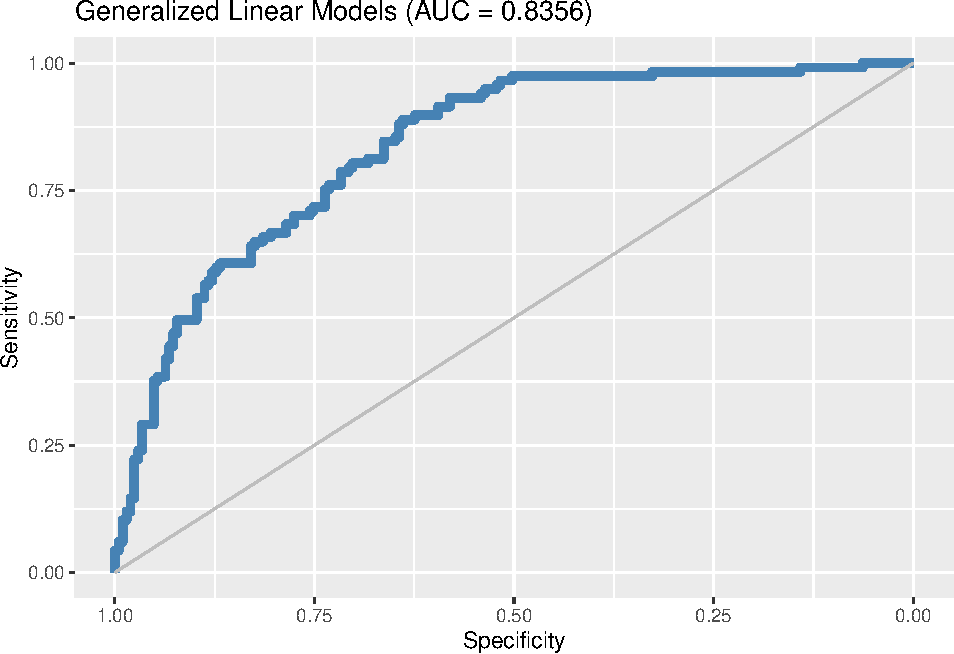
\includegraphics{06-Individual_Logistic_Models_files/figure-latex/Our first logistic model-1.pdf}

\begin{verbatim}
#> [1] 0.7701863

# Check for any errors
warnings()
\end{verbatim}

The results are consistent with similar results using Generalized Linear Models for this data set.

\subsection{How to use non-GLM models in logistic analysis}\label{how-to-use-non-glm-models-in-logistic-analysis}

The authors of the excellent book, Introduction to Statistical Learning, describe and demonstrate how non-GLM methods may be used in logistic analysis. They investigated Linear Discriminant Analysis, Quadratic Discriminant Analysis and K-Nearest Neighbors. We will look at a total of ten methods, though many more are possible.

\begin{figure}
\centering
\includegraphics{Images/GLM_warning.jpg}
\caption{Logistic warning}
\end{figure}

\subsection{Eight individual models for logistic data}\label{eight-individual-models-for-logistic-data}

\subsection{Adaboost}\label{adaboost}

\begin{Shaded}
\begin{Highlighting}[]

\CommentTok{\# Load the library}
\FunctionTok{library}\NormalTok{(MachineShop)}
\CommentTok{\#\textgreater{} }
\CommentTok{\#\textgreater{} Attaching package: \textquotesingle{}MachineShop\textquotesingle{}}
\CommentTok{\#\textgreater{} The following object is masked from \textquotesingle{}package:pROC\textquotesingle{}:}
\CommentTok{\#\textgreater{} }
\CommentTok{\#\textgreater{}     auc}
\CommentTok{\#\textgreater{} The following object is masked from \textquotesingle{}package:purrr\textquotesingle{}:}
\CommentTok{\#\textgreater{} }
\CommentTok{\#\textgreater{}     lift}
\CommentTok{\#\textgreater{} The following object is masked from \textquotesingle{}package:stats\textquotesingle{}:}
\CommentTok{\#\textgreater{} }
\CommentTok{\#\textgreater{}     ppr}
\FunctionTok{library}\NormalTok{(tidyverse)}
\FunctionTok{library}\NormalTok{(pROC)}

\CommentTok{\# Set initial values to 0}

\NormalTok{adaboost\_train\_accuracy }\OtherTok{\textless{}{-}} \DecValTok{0}
\NormalTok{adaboost\_test\_accuracy }\OtherTok{\textless{}{-}} \DecValTok{0}
\NormalTok{adaboost\_holdout\_accuracy }\OtherTok{\textless{}{-}} \DecValTok{0}
\NormalTok{adaboost\_duration }\OtherTok{\textless{}{-}} \DecValTok{0}
\NormalTok{adaboost\_table\_total }\OtherTok{\textless{}{-}} \DecValTok{0}

\CommentTok{\# Create the function}

\NormalTok{adaboost\_1 }\OtherTok{\textless{}{-}} \ControlFlowTok{function}\NormalTok{(data, colnum, numresamples, train\_amount, test\_amount)\{}
  
  \FunctionTok{colnames}\NormalTok{(data)[colnum] }\OtherTok{\textless{}{-}} \StringTok{"y"}
  
\NormalTok{  df }\OtherTok{\textless{}{-}}\NormalTok{ data }\SpecialCharTok{\%\textgreater{}\%}\NormalTok{ dplyr}\SpecialCharTok{::}\FunctionTok{relocate}\NormalTok{(y, }\AttributeTok{.after =} \FunctionTok{last\_col}\NormalTok{()) }\CommentTok{\# Moves the target column to the last column on the right}
  
\NormalTok{  df }\OtherTok{\textless{}{-}}\NormalTok{ df[}\FunctionTok{sample}\NormalTok{(}\DecValTok{1}\SpecialCharTok{:}\FunctionTok{nrow}\NormalTok{(df)), ] }\CommentTok{\# randomizes the rows}
  
  \CommentTok{\# Set up random resampling}
  
  \ControlFlowTok{for}\NormalTok{ (i }\ControlFlowTok{in} \DecValTok{1}\SpecialCharTok{:}\NormalTok{numresamples) \{}
    
\NormalTok{    index }\OtherTok{\textless{}{-}} \FunctionTok{sample}\NormalTok{(}\FunctionTok{c}\NormalTok{(}\DecValTok{1}\SpecialCharTok{:}\DecValTok{2}\NormalTok{), }\FunctionTok{nrow}\NormalTok{(df), }\AttributeTok{replace =} \ConstantTok{TRUE}\NormalTok{, }\AttributeTok{prob =} \FunctionTok{c}\NormalTok{(train\_amount, test\_amount))}
    
\NormalTok{    train }\OtherTok{\textless{}{-}}\NormalTok{ df[index }\SpecialCharTok{==} \DecValTok{1}\NormalTok{, ]}
\NormalTok{    test }\OtherTok{\textless{}{-}}\NormalTok{ df[index }\SpecialCharTok{==} \DecValTok{2}\NormalTok{, ]}
    
\NormalTok{    y\_train }\OtherTok{\textless{}{-}}\NormalTok{ train}\SpecialCharTok{$}\NormalTok{y}
\NormalTok{    y\_test }\OtherTok{\textless{}{-}}\NormalTok{ test}\SpecialCharTok{$}\NormalTok{y}
    
    \CommentTok{\# Fit the model to the training data, make predictions on the holdout data}
\NormalTok{adaboost\_train\_fit }\OtherTok{\textless{}{-}}\NormalTok{ MachineShop}\SpecialCharTok{::}\FunctionTok{fit}\NormalTok{(}\AttributeTok{formula =} \FunctionTok{as.factor}\NormalTok{(y) }\SpecialCharTok{\textasciitilde{}}\NormalTok{ ., }\AttributeTok{data =}\NormalTok{ train, }\AttributeTok{model =} \StringTok{"AdaBoostModel"}\NormalTok{)}

\NormalTok{adaboost\_train\_pred }\OtherTok{\textless{}{-}}\NormalTok{ stats}\SpecialCharTok{::}\FunctionTok{predict}\NormalTok{(adaboost\_train\_fit, train, }\AttributeTok{type =} \StringTok{"prob"}\NormalTok{)}
\NormalTok{adaboost\_train\_predictions }\OtherTok{\textless{}{-}} \FunctionTok{ifelse}\NormalTok{(adaboost\_train\_pred }\SpecialCharTok{\textgreater{}} \FloatTok{0.5}\NormalTok{, }\DecValTok{1}\NormalTok{, }\DecValTok{0}\NormalTok{)}
\NormalTok{adaboost\_train\_table }\OtherTok{\textless{}{-}} \FunctionTok{table}\NormalTok{(adaboost\_train\_predictions, y\_train)}
\NormalTok{adaboost\_train\_accuracy[i] }\OtherTok{\textless{}{-}}\NormalTok{ (adaboost\_train\_table[}\DecValTok{1}\NormalTok{, }\DecValTok{1}\NormalTok{] }\SpecialCharTok{+}\NormalTok{ adaboost\_train\_table[}\DecValTok{2}\NormalTok{, }\DecValTok{2}\NormalTok{]) }\SpecialCharTok{/} \FunctionTok{sum}\NormalTok{(adaboost\_train\_table)}
\NormalTok{adaboost\_train\_accuracy\_mean }\OtherTok{\textless{}{-}} \FunctionTok{mean}\NormalTok{(adaboost\_train\_accuracy)}
    
\NormalTok{adaboost\_test\_pred }\OtherTok{\textless{}{-}}\NormalTok{ stats}\SpecialCharTok{::}\FunctionTok{predict}\NormalTok{(adaboost\_train\_fit, test, }\AttributeTok{type =} \StringTok{"prob"}\NormalTok{)}
\NormalTok{adaboost\_test\_predictions }\OtherTok{\textless{}{-}} \FunctionTok{ifelse}\NormalTok{(adaboost\_test\_pred }\SpecialCharTok{\textgreater{}} \FloatTok{0.5}\NormalTok{, }\DecValTok{1}\NormalTok{, }\DecValTok{0}\NormalTok{)}
\NormalTok{adaboost\_test\_table }\OtherTok{\textless{}{-}} \FunctionTok{table}\NormalTok{(adaboost\_test\_predictions, y\_test)}
\NormalTok{adaboost\_test\_accuracy[i] }\OtherTok{\textless{}{-}}\NormalTok{ (adaboost\_test\_table[}\DecValTok{1}\NormalTok{, }\DecValTok{1}\NormalTok{] }\SpecialCharTok{+}\NormalTok{ adaboost\_test\_table[}\DecValTok{2}\NormalTok{, }\DecValTok{2}\NormalTok{]) }\SpecialCharTok{/} \FunctionTok{sum}\NormalTok{(adaboost\_test\_table)}
\NormalTok{adaboost\_test\_accuracy\_mean }\OtherTok{\textless{}{-}} \FunctionTok{mean}\NormalTok{(adaboost\_test\_accuracy)}

\NormalTok{adaboost\_roc\_obj }\OtherTok{\textless{}{-}}\NormalTok{ pROC}\SpecialCharTok{::}\FunctionTok{roc}\NormalTok{(}\FunctionTok{as.numeric}\NormalTok{(}\FunctionTok{c}\NormalTok{(test}\SpecialCharTok{$}\NormalTok{y)), }\FunctionTok{c}\NormalTok{(adaboost\_test\_pred))}
\NormalTok{adaboost\_auc }\OtherTok{\textless{}{-}} \FunctionTok{round}\NormalTok{((pROC}\SpecialCharTok{::}\FunctionTok{auc}\NormalTok{(}\FunctionTok{c}\NormalTok{(test}\SpecialCharTok{$}\NormalTok{y), }\FunctionTok{as.numeric}\NormalTok{(}\FunctionTok{c}\NormalTok{(adaboost\_test\_pred)) }\SpecialCharTok{{-}} \DecValTok{1}\NormalTok{)), }\DecValTok{4}\NormalTok{)}
\FunctionTok{print}\NormalTok{(pROC}\SpecialCharTok{::}\FunctionTok{ggroc}\NormalTok{(adaboost\_roc\_obj, }\AttributeTok{color =} \StringTok{"steelblue"}\NormalTok{, }\AttributeTok{size =} \DecValTok{2}\NormalTok{) }\SpecialCharTok{+}
\NormalTok{            ggplot2}\SpecialCharTok{::}\FunctionTok{ggtitle}\NormalTok{(}\FunctionTok{paste0}\NormalTok{(}\StringTok{"ADAboost Models "}\NormalTok{, }\StringTok{"(AUC = "}\NormalTok{, adaboost\_auc, }\StringTok{")"}\NormalTok{)) }\SpecialCharTok{+}
\NormalTok{            ggplot2}\SpecialCharTok{::}\FunctionTok{labs}\NormalTok{(}\AttributeTok{x =} \StringTok{"Specificity"}\NormalTok{, }\AttributeTok{y =} \StringTok{"Sensitivity"}\NormalTok{) }\SpecialCharTok{+}
\NormalTok{            ggplot2}\SpecialCharTok{::}\FunctionTok{annotate}\NormalTok{(}\StringTok{"segment"}\NormalTok{, }\AttributeTok{x =} \DecValTok{1}\NormalTok{, }\AttributeTok{xend =} \DecValTok{0}\NormalTok{, }\AttributeTok{y =} \DecValTok{0}\NormalTok{, }\AttributeTok{yend =} \DecValTok{1}\NormalTok{, }\AttributeTok{color =} \StringTok{"grey"}\NormalTok{)}
\NormalTok{    )}
    
\FunctionTok{return}\NormalTok{(adaboost\_test\_accuracy\_mean)}
    
\NormalTok{  \} }\CommentTok{\# closing brace for numresamples }
  
\NormalTok{\} }\CommentTok{\# Closing brace for the function}

\CommentTok{\# Test the function}
\FunctionTok{adaboost\_1}\NormalTok{(}\AttributeTok{data =}\NormalTok{ diabetes, }\AttributeTok{colnum =} \DecValTok{9}\NormalTok{, }\AttributeTok{numresamples =} \DecValTok{5}\NormalTok{, }\AttributeTok{train\_amount =} \FloatTok{0.60}\NormalTok{, }\AttributeTok{test\_amount =} \FloatTok{0.40}\NormalTok{)}
\CommentTok{\#\textgreater{} Warning in rgl.init(initValue, onlyNULL): RGL: unable to}
\CommentTok{\#\textgreater{} open X11 display}
\CommentTok{\#\textgreater{} Warning: \textquotesingle{}rgl.init\textquotesingle{} failed, running with \textquotesingle{}rgl.useNULL =}
\CommentTok{\#\textgreater{} TRUE\textquotesingle{}.}
\CommentTok{\#\textgreater{} Setting levels: control = 0, case = 1}
\CommentTok{\#\textgreater{} Setting direction: controls \textless{} cases}
\CommentTok{\#\textgreater{} Setting levels: control = 0, case = 1}
\CommentTok{\#\textgreater{} Setting direction: controls \textless{} cases}
\end{Highlighting}
\end{Shaded}

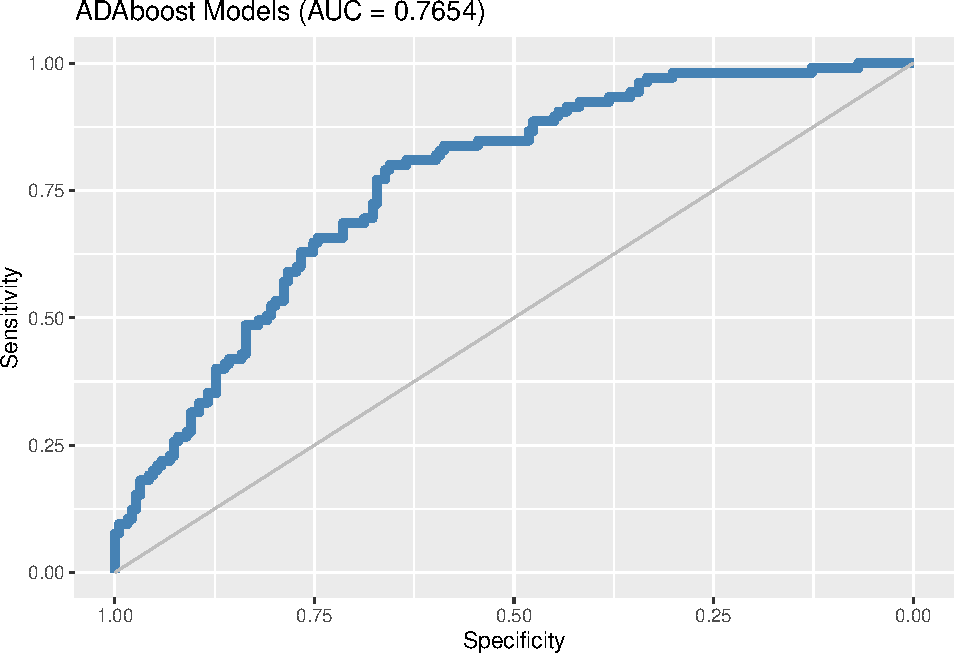
\includegraphics{06-Individual_Logistic_Models_files/figure-latex/ADABoost for logistic data-1.pdf}

\begin{verbatim}
#> [1] 0.7108844

# Check for any errors
warnings()
\end{verbatim}

\subsection{BayesGLM}\label{bayesglm-1}

\begin{Shaded}
\begin{Highlighting}[]

\CommentTok{\# Load the library}
\FunctionTok{library}\NormalTok{(arm)}
\CommentTok{\#\textgreater{} Loading required package: MASS}
\CommentTok{\#\textgreater{} }
\CommentTok{\#\textgreater{} Attaching package: \textquotesingle{}MASS\textquotesingle{}}
\CommentTok{\#\textgreater{} The following object is masked from \textquotesingle{}package:dplyr\textquotesingle{}:}
\CommentTok{\#\textgreater{} }
\CommentTok{\#\textgreater{}     select}
\CommentTok{\#\textgreater{} Loading required package: Matrix}
\CommentTok{\#\textgreater{} }
\CommentTok{\#\textgreater{} Attaching package: \textquotesingle{}Matrix\textquotesingle{}}
\CommentTok{\#\textgreater{} The following objects are masked from \textquotesingle{}package:tidyr\textquotesingle{}:}
\CommentTok{\#\textgreater{} }
\CommentTok{\#\textgreater{}     expand, pack, unpack}
\CommentTok{\#\textgreater{} Loading required package: lme4}
\CommentTok{\#\textgreater{} }
\CommentTok{\#\textgreater{} arm (Version 1.14{-}4, built: 2024{-}4{-}1)}
\CommentTok{\#\textgreater{} Working directory is /Users/russconte/Library/Mobile Documents/com\textasciitilde{}apple\textasciitilde{}CloudDocs/Documents/Machine Learning templates in R/EnsemblesBook}
\FunctionTok{library}\NormalTok{(tidyverse)}
\FunctionTok{library}\NormalTok{(pROC)}

\CommentTok{\# Set initial values to 0}

\NormalTok{bayesglm\_train\_accuracy }\OtherTok{\textless{}{-}} \DecValTok{0}
\NormalTok{bayesglm\_test\_accuracy }\OtherTok{\textless{}{-}} \DecValTok{0}
\NormalTok{bayesglm\_holdout\_accuracy }\OtherTok{\textless{}{-}} \DecValTok{0}
\NormalTok{bayesglm\_duration }\OtherTok{\textless{}{-}} \DecValTok{0}
\NormalTok{bayesglm\_table\_total }\OtherTok{\textless{}{-}} \DecValTok{0}

\CommentTok{\# Create the function}

\NormalTok{bayesglm\_1 }\OtherTok{\textless{}{-}} \ControlFlowTok{function}\NormalTok{(data, colnum, numresamples, train\_amount, test\_amount)\{}
  
  \FunctionTok{colnames}\NormalTok{(data)[colnum] }\OtherTok{\textless{}{-}} \StringTok{"y"}
  
\NormalTok{  df }\OtherTok{\textless{}{-}}\NormalTok{ data }\SpecialCharTok{\%\textgreater{}\%}\NormalTok{ dplyr}\SpecialCharTok{::}\FunctionTok{relocate}\NormalTok{(y, }\AttributeTok{.after =} \FunctionTok{last\_col}\NormalTok{()) }\CommentTok{\# Moves the target column to the last column on the right}
  
\NormalTok{  df }\OtherTok{\textless{}{-}}\NormalTok{ df[}\FunctionTok{sample}\NormalTok{(}\DecValTok{1}\SpecialCharTok{:}\FunctionTok{nrow}\NormalTok{(df)), ] }\CommentTok{\# randomizes the rows}
  
  \CommentTok{\# Set up random resampling}
  
  \ControlFlowTok{for}\NormalTok{ (i }\ControlFlowTok{in} \DecValTok{1}\SpecialCharTok{:}\NormalTok{numresamples) \{}
    
\NormalTok{    index }\OtherTok{\textless{}{-}} \FunctionTok{sample}\NormalTok{(}\FunctionTok{c}\NormalTok{(}\DecValTok{1}\SpecialCharTok{:}\DecValTok{2}\NormalTok{), }\FunctionTok{nrow}\NormalTok{(df), }\AttributeTok{replace =} \ConstantTok{TRUE}\NormalTok{, }\AttributeTok{prob =} \FunctionTok{c}\NormalTok{(train\_amount, test\_amount))}
    
\NormalTok{    train }\OtherTok{\textless{}{-}}\NormalTok{ df[index }\SpecialCharTok{==} \DecValTok{1}\NormalTok{, ]}
\NormalTok{    test }\OtherTok{\textless{}{-}}\NormalTok{ df[index }\SpecialCharTok{==} \DecValTok{2}\NormalTok{, ]}
    
\NormalTok{    y\_train }\OtherTok{\textless{}{-}}\NormalTok{ train}\SpecialCharTok{$}\NormalTok{y}
\NormalTok{    y\_test }\OtherTok{\textless{}{-}}\NormalTok{ test}\SpecialCharTok{$}\NormalTok{y}
    
    \CommentTok{\# Fit the model to the training data, make predictions on the holdout data}
\NormalTok{bayesglm\_train\_fit }\OtherTok{\textless{}{-}}\NormalTok{ arm}\SpecialCharTok{::}\FunctionTok{bayesglm}\NormalTok{(y }\SpecialCharTok{\textasciitilde{}}\NormalTok{ ., }\AttributeTok{data =}\NormalTok{ train, }\AttributeTok{family =}\NormalTok{ binomial)}
    
\NormalTok{bayesglm\_train\_pred }\OtherTok{\textless{}{-}}\NormalTok{ stats}\SpecialCharTok{::}\FunctionTok{predict}\NormalTok{(bayesglm\_train\_fit, train, }\AttributeTok{type =} \StringTok{"response"}\NormalTok{)}
\NormalTok{bayesglm\_train\_predictions }\OtherTok{\textless{}{-}} \FunctionTok{ifelse}\NormalTok{(bayesglm\_train\_pred }\SpecialCharTok{\textgreater{}} \FloatTok{0.5}\NormalTok{, }\DecValTok{1}\NormalTok{, }\DecValTok{0}\NormalTok{)}
\NormalTok{bayesglm\_train\_table }\OtherTok{\textless{}{-}} \FunctionTok{table}\NormalTok{(bayesglm\_train\_predictions, y\_train)}
\NormalTok{bayesglm\_train\_accuracy[i] }\OtherTok{\textless{}{-}}\NormalTok{ (bayesglm\_train\_table[}\DecValTok{1}\NormalTok{, }\DecValTok{1}\NormalTok{] }\SpecialCharTok{+}\NormalTok{ bayesglm\_train\_table[}\DecValTok{2}\NormalTok{, }\DecValTok{2}\NormalTok{]) }\SpecialCharTok{/} \FunctionTok{sum}\NormalTok{(bayesglm\_train\_table)}
\NormalTok{bayesglm\_train\_accuracy\_mean }\OtherTok{\textless{}{-}} \FunctionTok{mean}\NormalTok{(bayesglm\_train\_accuracy)}

\NormalTok{bayesglm\_test\_pred }\OtherTok{\textless{}{-}}\NormalTok{ stats}\SpecialCharTok{::}\FunctionTok{predict}\NormalTok{(bayesglm\_train\_fit, test, }\AttributeTok{type =} \StringTok{"response"}\NormalTok{)}
\NormalTok{bayesglm\_test\_predictions }\OtherTok{\textless{}{-}} \FunctionTok{ifelse}\NormalTok{(bayesglm\_test\_pred }\SpecialCharTok{\textgreater{}} \FloatTok{0.5}\NormalTok{, }\DecValTok{1}\NormalTok{, }\DecValTok{0}\NormalTok{)}
\NormalTok{bayesglm\_test\_table }\OtherTok{\textless{}{-}} \FunctionTok{table}\NormalTok{(bayesglm\_test\_predictions, y\_test)}

\NormalTok{bayesglm\_test\_accuracy[i] }\OtherTok{\textless{}{-}}\NormalTok{ (bayesglm\_test\_table[}\DecValTok{1}\NormalTok{, }\DecValTok{1}\NormalTok{] }\SpecialCharTok{+}\NormalTok{ bayesglm\_test\_table[}\DecValTok{2}\NormalTok{, }\DecValTok{2}\NormalTok{]) }\SpecialCharTok{/} \FunctionTok{sum}\NormalTok{(bayesglm\_test\_table)}
\NormalTok{bayesglm\_test\_accuracy\_mean }\OtherTok{\textless{}{-}} \FunctionTok{mean}\NormalTok{(bayesglm\_test\_accuracy)}

\NormalTok{bayesglm\_roc\_obj }\OtherTok{\textless{}{-}}\NormalTok{ pROC}\SpecialCharTok{::}\FunctionTok{roc}\NormalTok{(}\FunctionTok{as.numeric}\NormalTok{(}\FunctionTok{c}\NormalTok{(test}\SpecialCharTok{$}\NormalTok{y)), }\FunctionTok{c}\NormalTok{(bayesglm\_test\_pred))}
\NormalTok{bayesglm\_auc }\OtherTok{\textless{}{-}} \FunctionTok{round}\NormalTok{((pROC}\SpecialCharTok{::}\FunctionTok{auc}\NormalTok{(}\FunctionTok{c}\NormalTok{(test}\SpecialCharTok{$}\NormalTok{y), }\FunctionTok{as.numeric}\NormalTok{(}\FunctionTok{c}\NormalTok{(bayesglm\_test\_pred)) }\SpecialCharTok{{-}} \DecValTok{1}\NormalTok{)), }\DecValTok{4}\NormalTok{)}
\FunctionTok{print}\NormalTok{(pROC}\SpecialCharTok{::}\FunctionTok{ggroc}\NormalTok{(bayesglm\_roc\_obj, }\AttributeTok{color =} \StringTok{"steelblue"}\NormalTok{, }\AttributeTok{size =} \DecValTok{2}\NormalTok{) }\SpecialCharTok{+}
\NormalTok{            ggplot2}\SpecialCharTok{::}\FunctionTok{ggtitle}\NormalTok{(}\FunctionTok{paste0}\NormalTok{(}\StringTok{"Bayesglm Models "}\NormalTok{, }\StringTok{"(AUC = "}\NormalTok{, bayesglm\_auc, }\StringTok{")"}\NormalTok{)) }\SpecialCharTok{+}
\NormalTok{            ggplot2}\SpecialCharTok{::}\FunctionTok{labs}\NormalTok{(}\AttributeTok{x =} \StringTok{"Specificity"}\NormalTok{, }\AttributeTok{y =} \StringTok{"Sensitivity"}\NormalTok{) }\SpecialCharTok{+}
\NormalTok{            ggplot2}\SpecialCharTok{::}\FunctionTok{annotate}\NormalTok{(}\StringTok{"segment"}\NormalTok{, }\AttributeTok{x =} \DecValTok{1}\NormalTok{, }\AttributeTok{xend =} \DecValTok{0}\NormalTok{, }\AttributeTok{y =} \DecValTok{0}\NormalTok{, }\AttributeTok{yend =} \DecValTok{1}\NormalTok{, }\AttributeTok{color =} \StringTok{"grey"}\NormalTok{)}
\NormalTok{    )}
    
\FunctionTok{return}\NormalTok{(bayesglm\_test\_accuracy\_mean)}
    
\NormalTok{  \} }\CommentTok{\# closing brace for numresamples }
  
\NormalTok{\} }\CommentTok{\# Closing brace for the function}

\CommentTok{\# Test the function}
\FunctionTok{bayesglm\_1}\NormalTok{(}\AttributeTok{data =}\NormalTok{ diabetes, }\AttributeTok{colnum =} \DecValTok{9}\NormalTok{, }\AttributeTok{numresamples =} \DecValTok{5}\NormalTok{, }\AttributeTok{train\_amount =} \FloatTok{0.60}\NormalTok{, }\AttributeTok{test\_amount =} \FloatTok{0.40}\NormalTok{)}
\CommentTok{\#\textgreater{} Setting levels: control = 0, case = 1}
\CommentTok{\#\textgreater{} Setting direction: controls \textless{} cases}
\CommentTok{\#\textgreater{} Setting levels: control = 0, case = 1}
\CommentTok{\#\textgreater{} Setting direction: controls \textless{} cases}
\end{Highlighting}
\end{Shaded}

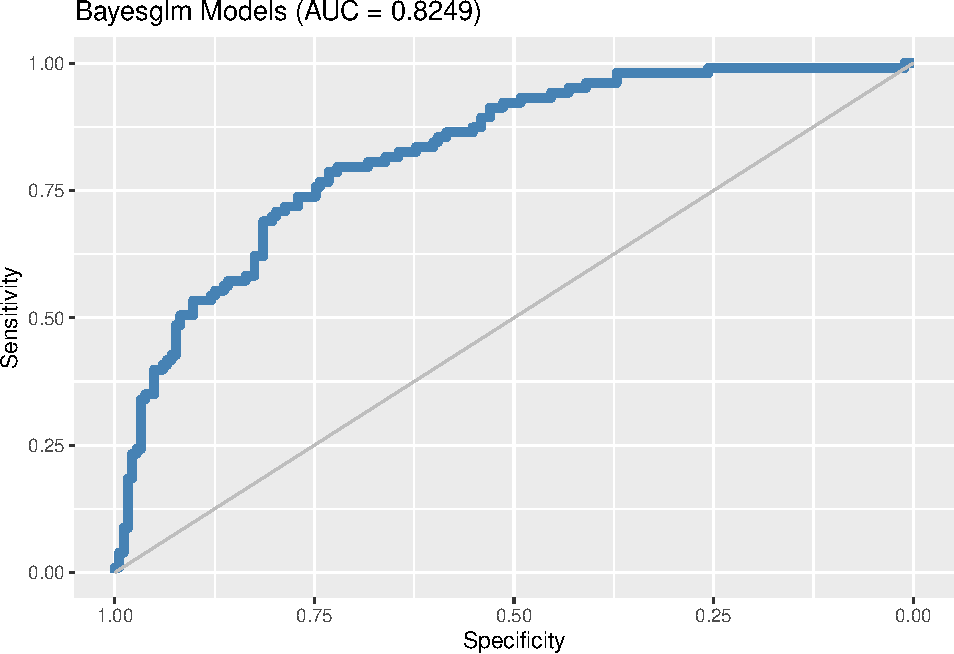
\includegraphics{06-Individual_Logistic_Models_files/figure-latex/BayesGLM model for logistic data-1.pdf}

\begin{verbatim}
#> [1] 0.7622378

# Check for any errors
warnings()
\end{verbatim}

\subsection{C50}\label{c50}

\begin{Shaded}
\begin{Highlighting}[]

\CommentTok{\# Load the library}
\FunctionTok{library}\NormalTok{(C50)}
\FunctionTok{library}\NormalTok{(tidyverse)}
\FunctionTok{library}\NormalTok{(pROC)}

\CommentTok{\# Set initial values to 0}

\NormalTok{C50\_train\_accuracy }\OtherTok{\textless{}{-}} \DecValTok{0}
\NormalTok{C50\_test\_accuracy }\OtherTok{\textless{}{-}} \DecValTok{0}
\NormalTok{C50\_holdout\_accuracy }\OtherTok{\textless{}{-}} \DecValTok{0}
\NormalTok{C50\_duration }\OtherTok{\textless{}{-}} \DecValTok{0}
\NormalTok{C50\_table\_total }\OtherTok{\textless{}{-}} \DecValTok{0}

\CommentTok{\# Create the function}

\NormalTok{C50\_1 }\OtherTok{\textless{}{-}} \ControlFlowTok{function}\NormalTok{(data, colnum, numresamples, train\_amount, test\_amount)\{}
  
  \FunctionTok{colnames}\NormalTok{(data)[colnum] }\OtherTok{\textless{}{-}} \StringTok{"y"}
  
\NormalTok{  df }\OtherTok{\textless{}{-}}\NormalTok{ data }\SpecialCharTok{\%\textgreater{}\%}\NormalTok{ dplyr}\SpecialCharTok{::}\FunctionTok{relocate}\NormalTok{(y, }\AttributeTok{.after =} \FunctionTok{last\_col}\NormalTok{()) }\CommentTok{\# Moves the target column to the last column on the right}
  
\NormalTok{  df }\OtherTok{\textless{}{-}}\NormalTok{ df[}\FunctionTok{sample}\NormalTok{(}\DecValTok{1}\SpecialCharTok{:}\FunctionTok{nrow}\NormalTok{(df)), ] }\CommentTok{\# randomizes the rows}
  
  \CommentTok{\# Set up random resampling}
  
  \ControlFlowTok{for}\NormalTok{ (i }\ControlFlowTok{in} \DecValTok{1}\SpecialCharTok{:}\NormalTok{numresamples) \{}
    
\NormalTok{    index }\OtherTok{\textless{}{-}} \FunctionTok{sample}\NormalTok{(}\FunctionTok{c}\NormalTok{(}\DecValTok{1}\SpecialCharTok{:}\DecValTok{2}\NormalTok{), }\FunctionTok{nrow}\NormalTok{(df), }\AttributeTok{replace =} \ConstantTok{TRUE}\NormalTok{, }\AttributeTok{prob =} \FunctionTok{c}\NormalTok{(train\_amount, test\_amount))}
    
\NormalTok{    train }\OtherTok{\textless{}{-}}\NormalTok{ df[index }\SpecialCharTok{==} \DecValTok{1}\NormalTok{, ]}
\NormalTok{    test }\OtherTok{\textless{}{-}}\NormalTok{ df[index }\SpecialCharTok{==} \DecValTok{2}\NormalTok{, ]}
    
\NormalTok{    y\_train }\OtherTok{\textless{}{-}}\NormalTok{ train}\SpecialCharTok{$}\NormalTok{y}
\NormalTok{    y\_test }\OtherTok{\textless{}{-}}\NormalTok{ test}\SpecialCharTok{$}\NormalTok{y}
    
    \CommentTok{\# Fit the model to the training data, make predictions on the holdout data}
\NormalTok{C50\_train\_fit }\OtherTok{\textless{}{-}}\NormalTok{ C50}\SpecialCharTok{::}\FunctionTok{C5.0}\NormalTok{(}\FunctionTok{as.factor}\NormalTok{(y\_train) }\SpecialCharTok{\textasciitilde{}}\NormalTok{ ., }\AttributeTok{data =}\NormalTok{ train)}

\NormalTok{C50\_train\_pred }\OtherTok{\textless{}{-}}\NormalTok{ stats}\SpecialCharTok{::}\FunctionTok{predict}\NormalTok{(C50\_train\_fit, train, }\AttributeTok{type =} \StringTok{"prob"}\NormalTok{)}
\NormalTok{C50\_train\_predictions }\OtherTok{\textless{}{-}} \FunctionTok{ifelse}\NormalTok{(C50\_train\_pred[, }\DecValTok{2}\NormalTok{] }\SpecialCharTok{\textgreater{}} \FloatTok{0.5}\NormalTok{, }\DecValTok{1}\NormalTok{, }\DecValTok{0}\NormalTok{)}
\NormalTok{C50\_train\_table }\OtherTok{\textless{}{-}} \FunctionTok{table}\NormalTok{(C50\_train\_predictions, y\_train)}
\NormalTok{C50\_train\_accuracy[i] }\OtherTok{\textless{}{-}}\NormalTok{ (C50\_train\_table[}\DecValTok{1}\NormalTok{, }\DecValTok{1}\NormalTok{] }\SpecialCharTok{+}\NormalTok{ C50\_train\_table[}\DecValTok{2}\NormalTok{, }\DecValTok{2}\NormalTok{]) }\SpecialCharTok{/} \FunctionTok{sum}\NormalTok{(C50\_train\_table)}
\NormalTok{C50\_train\_accuracy\_mean }\OtherTok{\textless{}{-}} \FunctionTok{mean}\NormalTok{(C50\_train\_accuracy)}

\NormalTok{C50\_test\_pred }\OtherTok{\textless{}{-}}\NormalTok{ stats}\SpecialCharTok{::}\FunctionTok{predict}\NormalTok{(C50\_train\_fit, test, }\AttributeTok{type =} \StringTok{"prob"}\NormalTok{)}
\NormalTok{C50\_test\_predictions }\OtherTok{\textless{}{-}} \FunctionTok{ifelse}\NormalTok{(C50\_test\_pred[, }\DecValTok{2}\NormalTok{] }\SpecialCharTok{\textgreater{}} \FloatTok{0.5}\NormalTok{, }\DecValTok{1}\NormalTok{, }\DecValTok{0}\NormalTok{)}
\NormalTok{C50\_test\_table }\OtherTok{\textless{}{-}} \FunctionTok{table}\NormalTok{(C50\_test\_predictions, y\_test)}
\NormalTok{C50\_test\_accuracy[i] }\OtherTok{\textless{}{-}}\NormalTok{ (C50\_test\_table[}\DecValTok{1}\NormalTok{, }\DecValTok{1}\NormalTok{] }\SpecialCharTok{+}\NormalTok{ C50\_test\_table[}\DecValTok{2}\NormalTok{, }\DecValTok{2}\NormalTok{]) }\SpecialCharTok{/} \FunctionTok{sum}\NormalTok{(C50\_test\_table)}
\NormalTok{C50\_test\_accuracy\_mean }\OtherTok{\textless{}{-}} \FunctionTok{mean}\NormalTok{(C50\_test\_accuracy)}

\NormalTok{C50\_roc\_obj }\OtherTok{\textless{}{-}}\NormalTok{ pROC}\SpecialCharTok{::}\FunctionTok{roc}\NormalTok{(}\FunctionTok{as.numeric}\NormalTok{(}\FunctionTok{c}\NormalTok{(test}\SpecialCharTok{$}\NormalTok{y)), }\FunctionTok{as.numeric}\NormalTok{(}\FunctionTok{c}\NormalTok{(C50\_test\_predictions)))}
\NormalTok{C50\_auc }\OtherTok{\textless{}{-}} \FunctionTok{round}\NormalTok{((pROC}\SpecialCharTok{::}\FunctionTok{auc}\NormalTok{(}\FunctionTok{c}\NormalTok{(test}\SpecialCharTok{$}\NormalTok{y), }\FunctionTok{as.numeric}\NormalTok{(}\FunctionTok{c}\NormalTok{(C50\_test\_predictions)) }\SpecialCharTok{{-}} \DecValTok{1}\NormalTok{)), }\DecValTok{4}\NormalTok{)}
\FunctionTok{print}\NormalTok{(pROC}\SpecialCharTok{::}\FunctionTok{ggroc}\NormalTok{(C50\_roc\_obj, }\AttributeTok{color =} \StringTok{"steelblue"}\NormalTok{, }\AttributeTok{size =} \DecValTok{2}\NormalTok{) }\SpecialCharTok{+}
\NormalTok{  ggplot2}\SpecialCharTok{::}\FunctionTok{ggtitle}\NormalTok{(}\FunctionTok{paste0}\NormalTok{(}\StringTok{"C50 ROC curve "}\NormalTok{, }\StringTok{"(AUC = "}\NormalTok{, C50\_auc, }\StringTok{")"}\NormalTok{)) }\SpecialCharTok{+}
\NormalTok{  ggplot2}\SpecialCharTok{::}\FunctionTok{labs}\NormalTok{(}\AttributeTok{x =} \StringTok{"Specificity"}\NormalTok{, }\AttributeTok{y =} \StringTok{"Sensitivity"}\NormalTok{) }\SpecialCharTok{+}
\NormalTok{  ggplot2}\SpecialCharTok{::}\FunctionTok{annotate}\NormalTok{(}\StringTok{"segment"}\NormalTok{, }\AttributeTok{x =} \DecValTok{1}\NormalTok{, }\AttributeTok{xend =} \DecValTok{0}\NormalTok{, }\AttributeTok{y =} \DecValTok{0}\NormalTok{, }\AttributeTok{yend =} \DecValTok{1}\NormalTok{, }\AttributeTok{color =} \StringTok{"grey"}\NormalTok{)}
\NormalTok{    )}
    
\FunctionTok{return}\NormalTok{(C50\_test\_accuracy\_mean)}
    
\NormalTok{  \} }\CommentTok{\# closing brace for numresamples }
  
\NormalTok{\} }\CommentTok{\# Closing brace for the function}

\CommentTok{\# Test the function}
\FunctionTok{C50\_1}\NormalTok{(}\AttributeTok{data =}\NormalTok{ diabetes, }\AttributeTok{colnum =} \DecValTok{9}\NormalTok{, }\AttributeTok{numresamples =} \DecValTok{5}\NormalTok{, }\AttributeTok{train\_amount =} \FloatTok{0.60}\NormalTok{, }\AttributeTok{test\_amount =} \FloatTok{0.40}\NormalTok{)}
\CommentTok{\#\textgreater{} Setting levels: control = 0, case = 1}
\CommentTok{\#\textgreater{} Setting direction: controls \textless{} cases}
\CommentTok{\#\textgreater{} Setting levels: control = 0, case = 1}
\CommentTok{\#\textgreater{} Setting direction: controls \textless{} cases}
\end{Highlighting}
\end{Shaded}

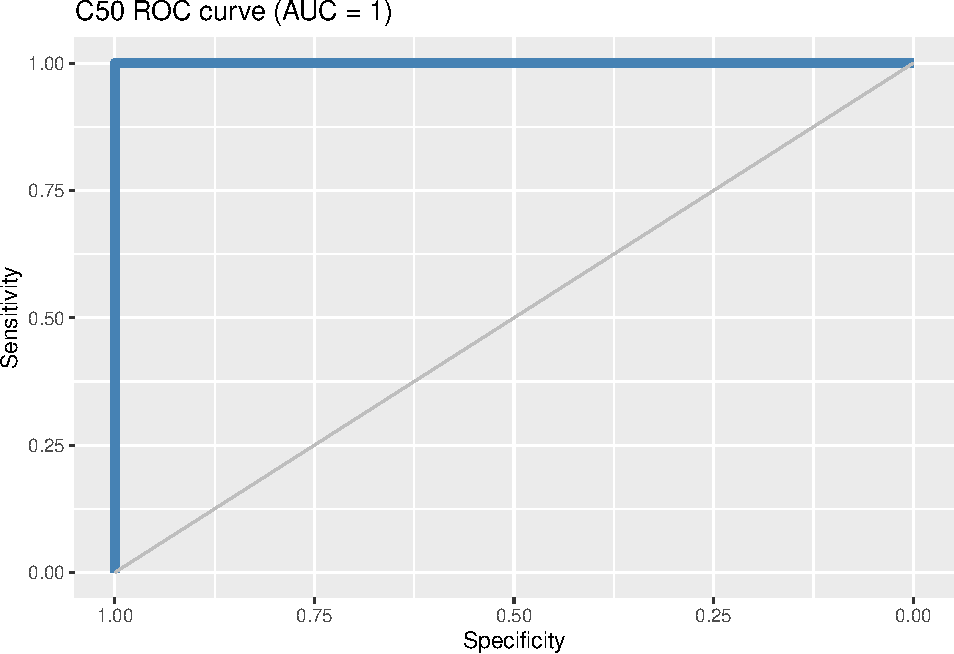
\includegraphics{06-Individual_Logistic_Models_files/figure-latex/C50 models for logistic data-1.pdf}

\begin{verbatim}
#> [1] 1

# Check for any errors
warnings()
\end{verbatim}

\subsection{Cubist}\label{cubist-1}

\begin{Shaded}
\begin{Highlighting}[]

\CommentTok{\# Load the library}
\FunctionTok{library}\NormalTok{(Cubist)}
\CommentTok{\#\textgreater{} Loading required package: lattice}
\FunctionTok{library}\NormalTok{(tidyverse)}
\FunctionTok{library}\NormalTok{(pROC)}

\CommentTok{\# Set initial values to 0}

\NormalTok{cubist\_train\_accuracy }\OtherTok{\textless{}{-}} \DecValTok{0}
\NormalTok{cubist\_test\_accuracy }\OtherTok{\textless{}{-}} \DecValTok{0}
\NormalTok{cubist\_holdout\_accuracy }\OtherTok{\textless{}{-}} \DecValTok{0}
\NormalTok{cubist\_duration }\OtherTok{\textless{}{-}} \DecValTok{0}
\NormalTok{cubist\_table\_total }\OtherTok{\textless{}{-}} \DecValTok{0}

\CommentTok{\# Create the function}

\NormalTok{cubist\_1 }\OtherTok{\textless{}{-}} \ControlFlowTok{function}\NormalTok{(data, colnum, numresamples, train\_amount, test\_amount)\{}
  
  \FunctionTok{colnames}\NormalTok{(data)[colnum] }\OtherTok{\textless{}{-}} \StringTok{"y"}
  
\NormalTok{  df }\OtherTok{\textless{}{-}}\NormalTok{ data }\SpecialCharTok{\%\textgreater{}\%}\NormalTok{ dplyr}\SpecialCharTok{::}\FunctionTok{relocate}\NormalTok{(y, }\AttributeTok{.after =} \FunctionTok{last\_col}\NormalTok{()) }\CommentTok{\# Moves the target column to the last column on the right}
  
\NormalTok{  df }\OtherTok{\textless{}{-}}\NormalTok{ df[}\FunctionTok{sample}\NormalTok{(}\DecValTok{1}\SpecialCharTok{:}\FunctionTok{nrow}\NormalTok{(df)), ] }\CommentTok{\# randomizes the rows}
  
  \CommentTok{\# Set up random resampling}
  
  \ControlFlowTok{for}\NormalTok{ (i }\ControlFlowTok{in} \DecValTok{1}\SpecialCharTok{:}\NormalTok{numresamples) \{}
    
\NormalTok{    index }\OtherTok{\textless{}{-}} \FunctionTok{sample}\NormalTok{(}\FunctionTok{c}\NormalTok{(}\DecValTok{1}\SpecialCharTok{:}\DecValTok{2}\NormalTok{), }\FunctionTok{nrow}\NormalTok{(df), }\AttributeTok{replace =} \ConstantTok{TRUE}\NormalTok{, }\AttributeTok{prob =} \FunctionTok{c}\NormalTok{(train\_amount, test\_amount))}
    
\NormalTok{    train }\OtherTok{\textless{}{-}}\NormalTok{ df[index }\SpecialCharTok{==} \DecValTok{1}\NormalTok{, ]}
\NormalTok{    test }\OtherTok{\textless{}{-}}\NormalTok{ df[index }\SpecialCharTok{==} \DecValTok{2}\NormalTok{, ]}
    
\NormalTok{    y\_train }\OtherTok{\textless{}{-}}\NormalTok{ train}\SpecialCharTok{$}\NormalTok{y}
\NormalTok{    y\_test }\OtherTok{\textless{}{-}}\NormalTok{ test}\SpecialCharTok{$}\NormalTok{y}
    
    \CommentTok{\# Fit the model to the training data, make predictions on the holdout data}
\NormalTok{cubist\_train\_fit }\OtherTok{\textless{}{-}}\NormalTok{ Cubist}\SpecialCharTok{::}\FunctionTok{cubist}\NormalTok{(}\AttributeTok{x =} \FunctionTok{as.data.frame}\NormalTok{(train), }\AttributeTok{y =}\NormalTok{ train}\SpecialCharTok{$}\NormalTok{y)}
    
\NormalTok{cubist\_train\_pred }\OtherTok{\textless{}{-}}\NormalTok{ stats}\SpecialCharTok{::}\FunctionTok{predict}\NormalTok{(cubist\_train\_fit, train, }\AttributeTok{type =} \StringTok{"prob"}\NormalTok{)}
\NormalTok{cubist\_train\_table }\OtherTok{\textless{}{-}} \FunctionTok{table}\NormalTok{(cubist\_train\_pred, y\_train)}
\NormalTok{cubist\_train\_accuracy[i] }\OtherTok{\textless{}{-}}\NormalTok{ (cubist\_train\_table[}\DecValTok{1}\NormalTok{, }\DecValTok{1}\NormalTok{] }\SpecialCharTok{+}\NormalTok{ cubist\_train\_table[}\DecValTok{2}\NormalTok{, }\DecValTok{2}\NormalTok{]) }\SpecialCharTok{/} \FunctionTok{sum}\NormalTok{(cubist\_train\_table)}
\NormalTok{cubist\_train\_accuracy\_mean }\OtherTok{\textless{}{-}} \FunctionTok{mean}\NormalTok{(cubist\_train\_accuracy)}

\NormalTok{cubist\_test\_pred }\OtherTok{\textless{}{-}}\NormalTok{ stats}\SpecialCharTok{::}\FunctionTok{predict}\NormalTok{(cubist\_train\_fit, test, }\AttributeTok{type =} \StringTok{"prob"}\NormalTok{)}
\NormalTok{cubist\_test\_table }\OtherTok{\textless{}{-}} \FunctionTok{table}\NormalTok{(cubist\_test\_pred, y\_test)}
\NormalTok{cubist\_test\_accuracy[i] }\OtherTok{\textless{}{-}}\NormalTok{ (cubist\_test\_table[}\DecValTok{1}\NormalTok{, }\DecValTok{1}\NormalTok{] }\SpecialCharTok{+}\NormalTok{ cubist\_test\_table[}\DecValTok{2}\NormalTok{, }\DecValTok{2}\NormalTok{]) }\SpecialCharTok{/} \FunctionTok{sum}\NormalTok{(cubist\_test\_table)}
\NormalTok{cubist\_test\_accuracy\_mean }\OtherTok{\textless{}{-}} \FunctionTok{mean}\NormalTok{(cubist\_test\_accuracy)}


\NormalTok{cubist\_roc\_obj }\OtherTok{\textless{}{-}}\NormalTok{ pROC}\SpecialCharTok{::}\FunctionTok{roc}\NormalTok{(}\FunctionTok{as.numeric}\NormalTok{(}\FunctionTok{c}\NormalTok{(test}\SpecialCharTok{$}\NormalTok{y)), }\FunctionTok{as.numeric}\NormalTok{(}\FunctionTok{c}\NormalTok{(cubist\_test\_pred)))}
\NormalTok{cubist\_auc }\OtherTok{\textless{}{-}} \FunctionTok{round}\NormalTok{((pROC}\SpecialCharTok{::}\FunctionTok{auc}\NormalTok{(}\FunctionTok{c}\NormalTok{(test}\SpecialCharTok{$}\NormalTok{y), }\FunctionTok{as.numeric}\NormalTok{(}\FunctionTok{c}\NormalTok{(cubist\_test\_pred)) }\SpecialCharTok{{-}} \DecValTok{1}\NormalTok{)), }\DecValTok{4}\NormalTok{)}
\FunctionTok{print}\NormalTok{(pROC}\SpecialCharTok{::}\FunctionTok{ggroc}\NormalTok{(cubist\_roc\_obj, }\AttributeTok{color =} \StringTok{"steelblue"}\NormalTok{, }\AttributeTok{size =} \DecValTok{2}\NormalTok{) }\SpecialCharTok{+}
\NormalTok{  ggplot2}\SpecialCharTok{::}\FunctionTok{ggtitle}\NormalTok{(}\FunctionTok{paste0}\NormalTok{(}\StringTok{"Cubist ROC curve "}\NormalTok{, }\StringTok{"(AUC = "}\NormalTok{, cubist\_auc, }\StringTok{")"}\NormalTok{)) }\SpecialCharTok{+}
\NormalTok{  ggplot2}\SpecialCharTok{::}\FunctionTok{labs}\NormalTok{(}\AttributeTok{x =} \StringTok{"Specificity"}\NormalTok{, }\AttributeTok{y =} \StringTok{"Sensitivity"}\NormalTok{) }\SpecialCharTok{+}
\NormalTok{  ggplot2}\SpecialCharTok{::}\FunctionTok{annotate}\NormalTok{(}\StringTok{"segment"}\NormalTok{, }\AttributeTok{x =} \DecValTok{1}\NormalTok{, }\AttributeTok{xend =} \DecValTok{0}\NormalTok{, }\AttributeTok{y =} \DecValTok{0}\NormalTok{, }\AttributeTok{yend =} \DecValTok{1}\NormalTok{, }\AttributeTok{color =} \StringTok{"grey"}\NormalTok{)}
\NormalTok{    )}
    
\FunctionTok{return}\NormalTok{(cubist\_test\_accuracy\_mean)}
    
\NormalTok{  \} }\CommentTok{\# closing brace for numresamples }
  
\NormalTok{\} }\CommentTok{\# Closing brace for the function}

\CommentTok{\# Test the function}
\FunctionTok{cubist\_1}\NormalTok{(}\AttributeTok{data =}\NormalTok{ diabetes, }\AttributeTok{colnum =} \DecValTok{9}\NormalTok{, }\AttributeTok{numresamples =} \DecValTok{5}\NormalTok{, }\AttributeTok{train\_amount =} \FloatTok{0.60}\NormalTok{, }\AttributeTok{test\_amount =} \FloatTok{0.40}\NormalTok{)}
\CommentTok{\#\textgreater{} Setting levels: control = 0, case = 1}
\CommentTok{\#\textgreater{} Setting direction: controls \textless{} cases}
\CommentTok{\#\textgreater{} Setting levels: control = 0, case = 1}
\CommentTok{\#\textgreater{} Setting direction: controls \textless{} cases}
\end{Highlighting}
\end{Shaded}

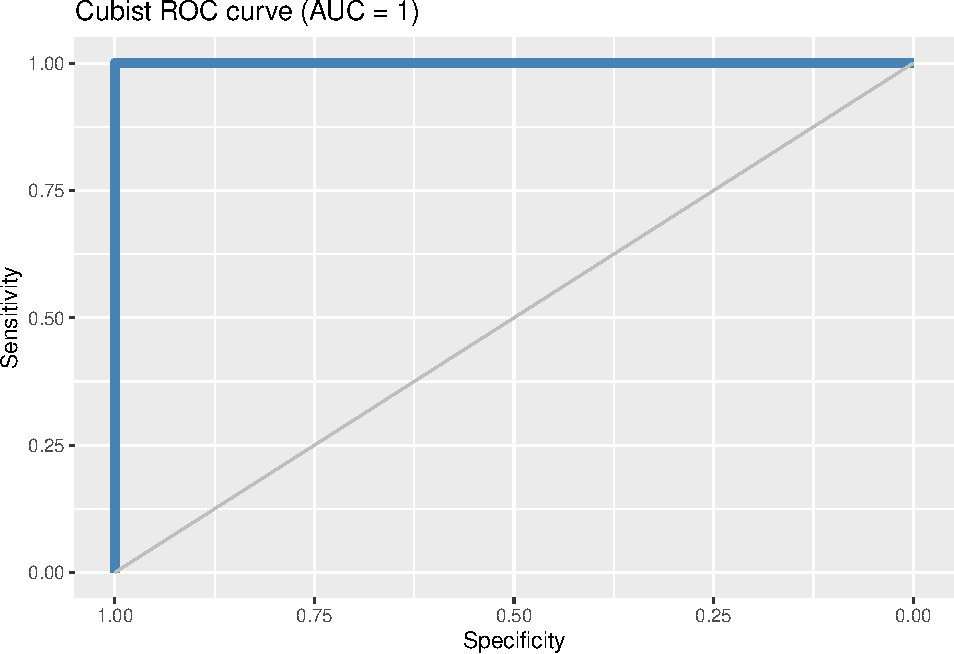
\includegraphics{06-Individual_Logistic_Models_files/figure-latex/Cubist model for logistic data-1.pdf}

\begin{verbatim}
#> [1] 1

# Check for any errors
warnings()
\end{verbatim}

\subsection{Gradient Boosted}\label{gradient-boosted-1}

\begin{Shaded}
\begin{Highlighting}[]

\CommentTok{\# Load the library}
\FunctionTok{library}\NormalTok{(gbm)}
\CommentTok{\#\textgreater{} Loaded gbm 2.1.9}
\CommentTok{\#\textgreater{} This version of gbm is no longer under development. Consider transitioning to gbm3, https://github.com/gbm{-}developers/gbm3}
\FunctionTok{library}\NormalTok{(tidyverse)}
\FunctionTok{library}\NormalTok{(pROC)}

\CommentTok{\# Set initial values to 0}

\NormalTok{gb\_train\_accuracy }\OtherTok{\textless{}{-}} \DecValTok{0}
\NormalTok{gb\_test\_accuracy }\OtherTok{\textless{}{-}} \DecValTok{0}
\NormalTok{gb\_holdout\_accuracy }\OtherTok{\textless{}{-}} \DecValTok{0}
\NormalTok{gb\_duration }\OtherTok{\textless{}{-}} \DecValTok{0}
\NormalTok{gb\_table\_total }\OtherTok{\textless{}{-}} \DecValTok{0}

\CommentTok{\# Create the function}

\NormalTok{gb\_1 }\OtherTok{\textless{}{-}} \ControlFlowTok{function}\NormalTok{(data, colnum, numresamples, train\_amount, test\_amount)\{}
  
  \FunctionTok{colnames}\NormalTok{(data)[colnum] }\OtherTok{\textless{}{-}} \StringTok{"y"}
  
\NormalTok{  df }\OtherTok{\textless{}{-}}\NormalTok{ data }\SpecialCharTok{\%\textgreater{}\%}\NormalTok{ dplyr}\SpecialCharTok{::}\FunctionTok{relocate}\NormalTok{(y, }\AttributeTok{.after =} \FunctionTok{last\_col}\NormalTok{()) }\CommentTok{\# Moves the target column to the last column on the right}
  
\NormalTok{  df }\OtherTok{\textless{}{-}}\NormalTok{ df[}\FunctionTok{sample}\NormalTok{(}\DecValTok{1}\SpecialCharTok{:}\FunctionTok{nrow}\NormalTok{(df)), ] }\CommentTok{\# randomizes the rows}
  
  \CommentTok{\# Set up random resampling}
  
  \ControlFlowTok{for}\NormalTok{ (i }\ControlFlowTok{in} \DecValTok{1}\SpecialCharTok{:}\NormalTok{numresamples) \{}
    
\NormalTok{    index }\OtherTok{\textless{}{-}} \FunctionTok{sample}\NormalTok{(}\FunctionTok{c}\NormalTok{(}\DecValTok{1}\SpecialCharTok{:}\DecValTok{2}\NormalTok{), }\FunctionTok{nrow}\NormalTok{(df), }\AttributeTok{replace =} \ConstantTok{TRUE}\NormalTok{, }\AttributeTok{prob =} \FunctionTok{c}\NormalTok{(train\_amount, test\_amount))}
    
\NormalTok{    train }\OtherTok{\textless{}{-}}\NormalTok{ df[index }\SpecialCharTok{==} \DecValTok{1}\NormalTok{, ]}
\NormalTok{    test }\OtherTok{\textless{}{-}}\NormalTok{ df[index }\SpecialCharTok{==} \DecValTok{2}\NormalTok{, ]}
    
\NormalTok{    y\_train }\OtherTok{\textless{}{-}}\NormalTok{ train}\SpecialCharTok{$}\NormalTok{y}
\NormalTok{    y\_test }\OtherTok{\textless{}{-}}\NormalTok{ test}\SpecialCharTok{$}\NormalTok{y}
    
    \CommentTok{\# Fit the model to the training data, make predictions on the holdout data}
\NormalTok{gb\_train\_fit }\OtherTok{\textless{}{-}}\NormalTok{ gbm}\SpecialCharTok{::}\FunctionTok{gbm}\NormalTok{(train}\SpecialCharTok{$}\NormalTok{y }\SpecialCharTok{\textasciitilde{}}\NormalTok{ ., }\AttributeTok{data =}\NormalTok{ train, }\AttributeTok{distribution =} \StringTok{"gaussian"}\NormalTok{, }\AttributeTok{n.trees =} \DecValTok{100}\NormalTok{, }\AttributeTok{shrinkage =} \FloatTok{0.1}\NormalTok{, }\AttributeTok{interaction.depth =} \DecValTok{10}\NormalTok{)}
    
\NormalTok{gb\_train\_pred }\OtherTok{\textless{}{-}}\NormalTok{ stats}\SpecialCharTok{::}\FunctionTok{predict}\NormalTok{(gb\_train\_fit, train, }\AttributeTok{type =} \StringTok{"response"}\NormalTok{)}
\NormalTok{gb\_train\_predictions }\OtherTok{\textless{}{-}} \FunctionTok{ifelse}\NormalTok{(gb\_train\_pred }\SpecialCharTok{\textgreater{}} \FloatTok{0.5}\NormalTok{, }\DecValTok{1}\NormalTok{, }\DecValTok{0}\NormalTok{)}
\NormalTok{gb\_train\_table }\OtherTok{\textless{}{-}} \FunctionTok{table}\NormalTok{(gb\_train\_predictions, y\_train)}
\NormalTok{gb\_train\_accuracy[i] }\OtherTok{\textless{}{-}}\NormalTok{ (gb\_train\_table[}\DecValTok{1}\NormalTok{, }\DecValTok{1}\NormalTok{] }\SpecialCharTok{+}\NormalTok{ gb\_train\_table[}\DecValTok{2}\NormalTok{, }\DecValTok{2}\NormalTok{]) }\SpecialCharTok{/} \FunctionTok{sum}\NormalTok{(gb\_train\_table)}
\NormalTok{gb\_train\_accuracy\_mean }\OtherTok{\textless{}{-}} \FunctionTok{mean}\NormalTok{(gb\_train\_accuracy)}

\NormalTok{gb\_test\_pred }\OtherTok{\textless{}{-}}\NormalTok{ stats}\SpecialCharTok{::}\FunctionTok{predict}\NormalTok{(gb\_train\_fit, test, }\AttributeTok{type =} \StringTok{"response"}\NormalTok{)}
\NormalTok{gb\_test\_predictions }\OtherTok{\textless{}{-}} \FunctionTok{ifelse}\NormalTok{(gb\_test\_pred }\SpecialCharTok{\textgreater{}} \FloatTok{0.5}\NormalTok{, }\DecValTok{1}\NormalTok{, }\DecValTok{0}\NormalTok{)}
\NormalTok{gb\_test\_table }\OtherTok{\textless{}{-}} \FunctionTok{table}\NormalTok{(gb\_test\_predictions, y\_test)}
\NormalTok{gb\_test\_accuracy[i] }\OtherTok{\textless{}{-}}\NormalTok{ (gb\_test\_table[}\DecValTok{1}\NormalTok{, }\DecValTok{1}\NormalTok{] }\SpecialCharTok{+}\NormalTok{ gb\_test\_table[}\DecValTok{2}\NormalTok{, }\DecValTok{2}\NormalTok{]) }\SpecialCharTok{/} \FunctionTok{sum}\NormalTok{(gb\_test\_table)}
\NormalTok{gb\_test\_accuracy\_mean }\OtherTok{\textless{}{-}} \FunctionTok{mean}\NormalTok{(gb\_test\_accuracy)}

\NormalTok{gb\_roc\_obj }\OtherTok{\textless{}{-}}\NormalTok{ pROC}\SpecialCharTok{::}\FunctionTok{roc}\NormalTok{(}\FunctionTok{as.numeric}\NormalTok{(}\FunctionTok{c}\NormalTok{(test}\SpecialCharTok{$}\NormalTok{y)), }\FunctionTok{as.numeric}\NormalTok{(}\FunctionTok{c}\NormalTok{(gb\_test\_pred)))}
\NormalTok{gb\_auc }\OtherTok{\textless{}{-}} \FunctionTok{round}\NormalTok{((pROC}\SpecialCharTok{::}\FunctionTok{auc}\NormalTok{(}\FunctionTok{c}\NormalTok{(test}\SpecialCharTok{$}\NormalTok{y), }\FunctionTok{as.numeric}\NormalTok{(}\FunctionTok{c}\NormalTok{(gb\_test\_pred)) }\SpecialCharTok{{-}} \DecValTok{1}\NormalTok{)), }\DecValTok{4}\NormalTok{)}
\FunctionTok{print}\NormalTok{(pROC}\SpecialCharTok{::}\FunctionTok{ggroc}\NormalTok{(gb\_roc\_obj, }\AttributeTok{color =} \StringTok{"steelblue"}\NormalTok{, }\AttributeTok{size =} \DecValTok{2}\NormalTok{) }\SpecialCharTok{+}
\NormalTok{  ggplot2}\SpecialCharTok{::}\FunctionTok{ggtitle}\NormalTok{(}\FunctionTok{paste0}\NormalTok{(}\StringTok{"Gradient Boosted ROC curve "}\NormalTok{, }\StringTok{"(AUC = "}\NormalTok{, gb\_auc, }\StringTok{")"}\NormalTok{)) }\SpecialCharTok{+}
\NormalTok{  ggplot2}\SpecialCharTok{::}\FunctionTok{labs}\NormalTok{(}\AttributeTok{x =} \StringTok{"Specificity"}\NormalTok{, }\AttributeTok{y =} \StringTok{"Sensitivity"}\NormalTok{) }\SpecialCharTok{+}
\NormalTok{  ggplot2}\SpecialCharTok{::}\FunctionTok{annotate}\NormalTok{(}\StringTok{"segment"}\NormalTok{, }\AttributeTok{x =} \DecValTok{1}\NormalTok{, }\AttributeTok{xend =} \DecValTok{0}\NormalTok{, }\AttributeTok{y =} \DecValTok{0}\NormalTok{, }\AttributeTok{yend =} \DecValTok{1}\NormalTok{, }\AttributeTok{color =} \StringTok{"grey"}\NormalTok{)}
\NormalTok{    )}
    
\FunctionTok{return}\NormalTok{(gb\_test\_accuracy\_mean)}
    
\NormalTok{  \} }\CommentTok{\# closing brace for numresamples }
  
\NormalTok{\} }\CommentTok{\# Closing brace for the function}

\CommentTok{\# Test the function}
\FunctionTok{gb\_1}\NormalTok{(}\AttributeTok{data =}\NormalTok{ diabetes, }\AttributeTok{colnum =} \DecValTok{9}\NormalTok{, }\AttributeTok{numresamples =} \DecValTok{5}\NormalTok{, }\AttributeTok{train\_amount =} \FloatTok{0.60}\NormalTok{, }\AttributeTok{test\_amount =} \FloatTok{0.40}\NormalTok{)}
\CommentTok{\#\textgreater{} Using 100 trees...}
\CommentTok{\#\textgreater{} Using 100 trees...}
\CommentTok{\#\textgreater{} Setting levels: control = 0, case = 1}
\CommentTok{\#\textgreater{} Setting direction: controls \textless{} cases}
\CommentTok{\#\textgreater{} Setting levels: control = 0, case = 1}
\CommentTok{\#\textgreater{} Setting direction: controls \textless{} cases}
\end{Highlighting}
\end{Shaded}

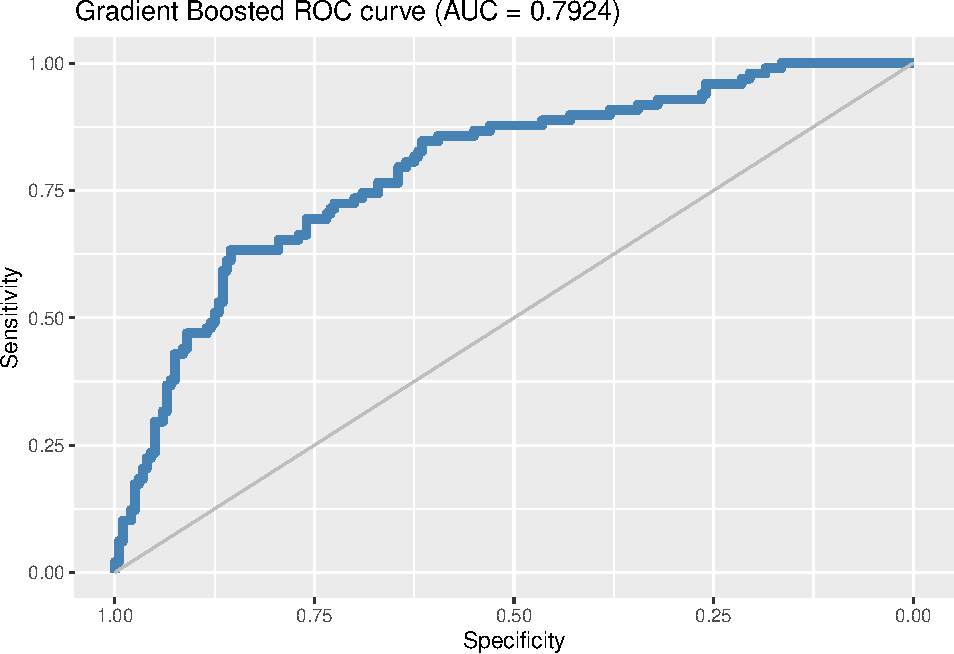
\includegraphics{06-Individual_Logistic_Models_files/figure-latex/Gradient Boosted model for logistic data-1.pdf}

\begin{verbatim}
#> [1] 0.7751678

# Check for any errors
warnings()
\end{verbatim}

\subsection{Random Forest}\label{random-forest-2}

\begin{Shaded}
\begin{Highlighting}[]

\CommentTok{\# Load the library}
\FunctionTok{library}\NormalTok{(randomForest)}
\CommentTok{\#\textgreater{} randomForest 4.7{-}1.1}
\CommentTok{\#\textgreater{} Type rfNews() to see new features/changes/bug fixes.}
\CommentTok{\#\textgreater{} }
\CommentTok{\#\textgreater{} Attaching package: \textquotesingle{}randomForest\textquotesingle{}}
\CommentTok{\#\textgreater{} The following object is masked from \textquotesingle{}package:dplyr\textquotesingle{}:}
\CommentTok{\#\textgreater{} }
\CommentTok{\#\textgreater{}     combine}
\CommentTok{\#\textgreater{} The following object is masked from \textquotesingle{}package:ggplot2\textquotesingle{}:}
\CommentTok{\#\textgreater{} }
\CommentTok{\#\textgreater{}     margin}
\FunctionTok{library}\NormalTok{(tidyverse)}
\FunctionTok{library}\NormalTok{(pROC)}

\CommentTok{\# Set initial values to 0}

\NormalTok{rf\_train\_accuracy }\OtherTok{\textless{}{-}} \DecValTok{0}
\NormalTok{rf\_test\_accuracy }\OtherTok{\textless{}{-}} \DecValTok{0}
\NormalTok{rf\_holdout\_accuracy }\OtherTok{\textless{}{-}} \DecValTok{0}
\NormalTok{rf\_duration }\OtherTok{\textless{}{-}} \DecValTok{0}
\NormalTok{rf\_table\_total }\OtherTok{\textless{}{-}} \DecValTok{0}

\CommentTok{\# Create the function}

\NormalTok{rf\_1 }\OtherTok{\textless{}{-}} \ControlFlowTok{function}\NormalTok{(data, colnum, numresamples, train\_amount, test\_amount)\{}
  
  \FunctionTok{colnames}\NormalTok{(data)[colnum] }\OtherTok{\textless{}{-}} \StringTok{"y"}
  
\NormalTok{  df }\OtherTok{\textless{}{-}}\NormalTok{ data }\SpecialCharTok{\%\textgreater{}\%}\NormalTok{ dplyr}\SpecialCharTok{::}\FunctionTok{relocate}\NormalTok{(y, }\AttributeTok{.after =} \FunctionTok{last\_col}\NormalTok{()) }\CommentTok{\# Moves the target column to the last column on the right}
  
\NormalTok{  df }\OtherTok{\textless{}{-}}\NormalTok{ df[}\FunctionTok{sample}\NormalTok{(}\DecValTok{1}\SpecialCharTok{:}\FunctionTok{nrow}\NormalTok{(df)), ] }\CommentTok{\# randomizes the rows}
  
  \CommentTok{\# Set up random resampling}
  
  \ControlFlowTok{for}\NormalTok{ (i }\ControlFlowTok{in} \DecValTok{1}\SpecialCharTok{:}\NormalTok{numresamples) \{}
    
\NormalTok{    index }\OtherTok{\textless{}{-}} \FunctionTok{sample}\NormalTok{(}\FunctionTok{c}\NormalTok{(}\DecValTok{1}\SpecialCharTok{:}\DecValTok{2}\NormalTok{), }\FunctionTok{nrow}\NormalTok{(df), }\AttributeTok{replace =} \ConstantTok{TRUE}\NormalTok{, }\AttributeTok{prob =} \FunctionTok{c}\NormalTok{(train\_amount, test\_amount))}
    
\NormalTok{    train }\OtherTok{\textless{}{-}}\NormalTok{ df[index }\SpecialCharTok{==} \DecValTok{1}\NormalTok{, ]}
\NormalTok{    test }\OtherTok{\textless{}{-}}\NormalTok{ df[index }\SpecialCharTok{==} \DecValTok{2}\NormalTok{, ]}
    
\NormalTok{    y\_train }\OtherTok{\textless{}{-}}\NormalTok{ train}\SpecialCharTok{$}\NormalTok{y}
\NormalTok{    y\_test }\OtherTok{\textless{}{-}}\NormalTok{ test}\SpecialCharTok{$}\NormalTok{y}
    
    \CommentTok{\# Fit the model to the training data, make predictions on the holdout data}
\NormalTok{rf\_train\_fit }\OtherTok{\textless{}{-}} \FunctionTok{randomForest}\NormalTok{(}\AttributeTok{x =}\NormalTok{ train, }\AttributeTok{y =} \FunctionTok{as.factor}\NormalTok{(y\_train), }\AttributeTok{data =}\NormalTok{ df)}
    
\NormalTok{rf\_train\_pred }\OtherTok{\textless{}{-}}\NormalTok{ stats}\SpecialCharTok{::}\FunctionTok{predict}\NormalTok{(rf\_train\_fit, train, }\AttributeTok{type =} \StringTok{"prob"}\NormalTok{)}
\NormalTok{rf\_train\_probabilities }\OtherTok{\textless{}{-}} \FunctionTok{ifelse}\NormalTok{(rf\_train\_pred }\SpecialCharTok{\textgreater{}} \FloatTok{0.50}\NormalTok{, }\DecValTok{1}\NormalTok{, }\DecValTok{0}\NormalTok{)[, }\DecValTok{2}\NormalTok{]}
\NormalTok{rf\_train\_table }\OtherTok{\textless{}{-}} \FunctionTok{table}\NormalTok{(rf\_train\_probabilities, y\_train)}
\NormalTok{rf\_train\_accuracy[i] }\OtherTok{\textless{}{-}}\NormalTok{ (rf\_train\_table[}\DecValTok{1}\NormalTok{, }\DecValTok{1}\NormalTok{] }\SpecialCharTok{+}\NormalTok{ rf\_train\_table[}\DecValTok{2}\NormalTok{, }\DecValTok{2}\NormalTok{]) }\SpecialCharTok{/} \FunctionTok{sum}\NormalTok{(rf\_train\_table)}
\NormalTok{rf\_train\_accuracy\_mean }\OtherTok{\textless{}{-}} \FunctionTok{mean}\NormalTok{(rf\_train\_accuracy)}

\NormalTok{rf\_test\_pred }\OtherTok{\textless{}{-}}\NormalTok{ stats}\SpecialCharTok{::}\FunctionTok{predict}\NormalTok{(rf\_train\_fit, test, }\AttributeTok{type =} \StringTok{"prob"}\NormalTok{)}
\NormalTok{rf\_test\_probabilities }\OtherTok{\textless{}{-}} \FunctionTok{ifelse}\NormalTok{(rf\_test\_pred }\SpecialCharTok{\textgreater{}} \FloatTok{0.50}\NormalTok{, }\DecValTok{1}\NormalTok{, }\DecValTok{0}\NormalTok{)[, }\DecValTok{2}\NormalTok{]}
\NormalTok{rf\_test\_table }\OtherTok{\textless{}{-}} \FunctionTok{table}\NormalTok{(rf\_test\_probabilities, y\_test)}
\NormalTok{rf\_test\_accuracy[i] }\OtherTok{\textless{}{-}}\NormalTok{ (rf\_test\_table[}\DecValTok{1}\NormalTok{, }\DecValTok{1}\NormalTok{] }\SpecialCharTok{+}\NormalTok{ rf\_test\_table[}\DecValTok{2}\NormalTok{, }\DecValTok{2}\NormalTok{]) }\SpecialCharTok{/} \FunctionTok{sum}\NormalTok{(rf\_test\_table)}
\NormalTok{rf\_test\_accuracy\_mean }\OtherTok{\textless{}{-}} \FunctionTok{mean}\NormalTok{(rf\_test\_accuracy)}

\NormalTok{rf\_roc\_obj }\OtherTok{\textless{}{-}}\NormalTok{ pROC}\SpecialCharTok{::}\FunctionTok{roc}\NormalTok{(}\FunctionTok{as.numeric}\NormalTok{(}\FunctionTok{c}\NormalTok{(test}\SpecialCharTok{$}\NormalTok{y)), }\FunctionTok{as.numeric}\NormalTok{(}\FunctionTok{c}\NormalTok{(rf\_test\_probabilities)))}
\NormalTok{rf\_auc }\OtherTok{\textless{}{-}} \FunctionTok{round}\NormalTok{((pROC}\SpecialCharTok{::}\FunctionTok{auc}\NormalTok{(}\FunctionTok{c}\NormalTok{(test}\SpecialCharTok{$}\NormalTok{y), }\FunctionTok{as.numeric}\NormalTok{(}\FunctionTok{c}\NormalTok{(rf\_test\_probabilities)) }\SpecialCharTok{{-}} \DecValTok{1}\NormalTok{)), }\DecValTok{4}\NormalTok{)}
\FunctionTok{print}\NormalTok{(pROC}\SpecialCharTok{::}\FunctionTok{ggroc}\NormalTok{(rf\_roc\_obj, }\AttributeTok{color =} \StringTok{"steelblue"}\NormalTok{, }\AttributeTok{size =} \DecValTok{2}\NormalTok{) }\SpecialCharTok{+}
\NormalTok{  ggplot2}\SpecialCharTok{::}\FunctionTok{ggtitle}\NormalTok{(}\FunctionTok{paste0}\NormalTok{(}\StringTok{"Random Forest "}\NormalTok{, }\StringTok{"(AUC = "}\NormalTok{, rf\_auc, }\StringTok{")"}\NormalTok{)) }\SpecialCharTok{+}
\NormalTok{  ggplot2}\SpecialCharTok{::}\FunctionTok{labs}\NormalTok{(}\AttributeTok{x =} \StringTok{"Specificity"}\NormalTok{, }\AttributeTok{y =} \StringTok{"Sensitivity"}\NormalTok{) }\SpecialCharTok{+}
\NormalTok{  ggplot2}\SpecialCharTok{::}\FunctionTok{annotate}\NormalTok{(}\StringTok{"segment"}\NormalTok{, }\AttributeTok{x =} \DecValTok{1}\NormalTok{, }\AttributeTok{xend =} \DecValTok{0}\NormalTok{, }\AttributeTok{y =} \DecValTok{0}\NormalTok{, }\AttributeTok{yend =} \DecValTok{1}\NormalTok{, }\AttributeTok{color =} \StringTok{"grey"}\NormalTok{)}
\NormalTok{    )}
    
\FunctionTok{return}\NormalTok{(rf\_test\_accuracy\_mean)}
    
\NormalTok{  \} }\CommentTok{\# closing brace for numresamples }
  
\NormalTok{\} }\CommentTok{\# Closing brace for the function}

\CommentTok{\# Test the function}
\FunctionTok{rf\_1}\NormalTok{(}\AttributeTok{data =}\NormalTok{ diabetes, }\AttributeTok{colnum =} \DecValTok{9}\NormalTok{, }\AttributeTok{numresamples =} \DecValTok{5}\NormalTok{, }\AttributeTok{train\_amount =} \FloatTok{0.60}\NormalTok{, }\AttributeTok{test\_amount =} \FloatTok{0.40}\NormalTok{)}
\CommentTok{\#\textgreater{} Setting levels: control = 0, case = 1}
\CommentTok{\#\textgreater{} Setting direction: controls \textless{} cases}
\CommentTok{\#\textgreater{} Setting levels: control = 0, case = 1}
\CommentTok{\#\textgreater{} Setting direction: controls \textless{} cases}
\end{Highlighting}
\end{Shaded}

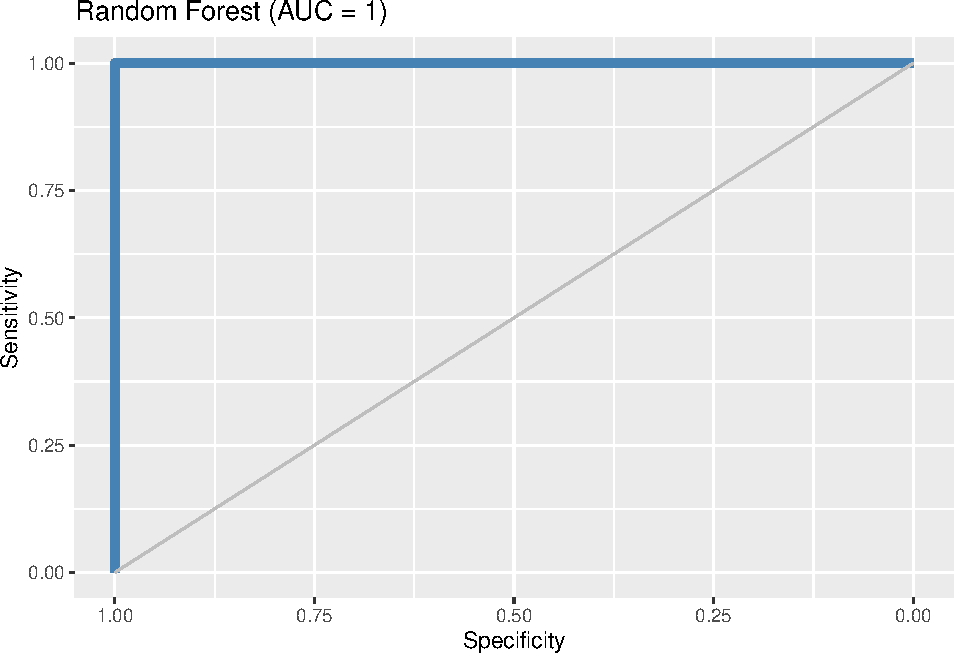
\includegraphics{06-Individual_Logistic_Models_files/figure-latex/Random Forest for logistic data-1.pdf}

\begin{verbatim}
#> [1] 1

# Check for any errors
warnings()
\end{verbatim}

\subsection{Support Vector Machines}\label{support-vector-machines-2}

\begin{Shaded}
\begin{Highlighting}[]

\CommentTok{\# Load the library}
\FunctionTok{library}\NormalTok{(e1071)}
\FunctionTok{library}\NormalTok{(tidyverse)}
\FunctionTok{library}\NormalTok{(pROC)}

\CommentTok{\# Set initial values to 0}

\NormalTok{svm\_train\_accuracy }\OtherTok{\textless{}{-}} \DecValTok{0}
\NormalTok{svm\_test\_accuracy }\OtherTok{\textless{}{-}} \DecValTok{0}
\NormalTok{svm\_holdout\_accuracy }\OtherTok{\textless{}{-}} \DecValTok{0}
\NormalTok{svm\_duration }\OtherTok{\textless{}{-}} \DecValTok{0}
\NormalTok{svm\_table\_total }\OtherTok{\textless{}{-}} \DecValTok{0}

\CommentTok{\# Create the function}

\NormalTok{svm\_1 }\OtherTok{\textless{}{-}} \ControlFlowTok{function}\NormalTok{(data, colnum, numresamples, train\_amount, test\_amount)\{}
  
  \FunctionTok{colnames}\NormalTok{(data)[colnum] }\OtherTok{\textless{}{-}} \StringTok{"y"}
  
\NormalTok{  df }\OtherTok{\textless{}{-}}\NormalTok{ data }\SpecialCharTok{\%\textgreater{}\%}\NormalTok{ dplyr}\SpecialCharTok{::}\FunctionTok{relocate}\NormalTok{(y, }\AttributeTok{.after =} \FunctionTok{last\_col}\NormalTok{()) }\CommentTok{\# Moves the target column to the last column on the right}
  
\NormalTok{  df }\OtherTok{\textless{}{-}}\NormalTok{ df[}\FunctionTok{sample}\NormalTok{(}\DecValTok{1}\SpecialCharTok{:}\FunctionTok{nrow}\NormalTok{(df)), ] }\CommentTok{\# randomizes the rows}
  
  \CommentTok{\# Set up random resampling}
  
  \ControlFlowTok{for}\NormalTok{ (i }\ControlFlowTok{in} \DecValTok{1}\SpecialCharTok{:}\NormalTok{numresamples) \{}
    
\NormalTok{    index }\OtherTok{\textless{}{-}} \FunctionTok{sample}\NormalTok{(}\FunctionTok{c}\NormalTok{(}\DecValTok{1}\SpecialCharTok{:}\DecValTok{2}\NormalTok{), }\FunctionTok{nrow}\NormalTok{(df), }\AttributeTok{replace =} \ConstantTok{TRUE}\NormalTok{, }\AttributeTok{prob =} \FunctionTok{c}\NormalTok{(train\_amount, test\_amount))}
    
\NormalTok{    train }\OtherTok{\textless{}{-}}\NormalTok{ df[index }\SpecialCharTok{==} \DecValTok{1}\NormalTok{, ]}
\NormalTok{    test }\OtherTok{\textless{}{-}}\NormalTok{ df[index }\SpecialCharTok{==} \DecValTok{2}\NormalTok{, ]}
    
\NormalTok{    y\_train }\OtherTok{\textless{}{-}}\NormalTok{ train}\SpecialCharTok{$}\NormalTok{y}
\NormalTok{    y\_test }\OtherTok{\textless{}{-}}\NormalTok{ test}\SpecialCharTok{$}\NormalTok{y}
    
    \CommentTok{\# Fit the model to the training data, make predictions on the holdout data}
\NormalTok{svm\_train\_fit }\OtherTok{\textless{}{-}}\NormalTok{ e1071}\SpecialCharTok{::}\FunctionTok{svm}\NormalTok{(}\FunctionTok{as.factor}\NormalTok{(y) }\SpecialCharTok{\textasciitilde{}}\NormalTok{ ., }\AttributeTok{data =}\NormalTok{ train)}
    
\NormalTok{svm\_train\_pred }\OtherTok{\textless{}{-}}\NormalTok{ stats}\SpecialCharTok{::}\FunctionTok{predict}\NormalTok{(svm\_train\_fit, train, }\AttributeTok{type =} \StringTok{"prob"}\NormalTok{)}
\NormalTok{svm\_train\_table }\OtherTok{\textless{}{-}} \FunctionTok{table}\NormalTok{(svm\_train\_pred, y\_train)}
\NormalTok{svm\_train\_accuracy[i] }\OtherTok{\textless{}{-}}\NormalTok{ (svm\_train\_table[}\DecValTok{1}\NormalTok{, }\DecValTok{1}\NormalTok{] }\SpecialCharTok{+}\NormalTok{ svm\_train\_table[}\DecValTok{2}\NormalTok{, }\DecValTok{2}\NormalTok{]) }\SpecialCharTok{/} \FunctionTok{sum}\NormalTok{(svm\_train\_table)}
\NormalTok{svm\_train\_accuracy\_mean }\OtherTok{\textless{}{-}} \FunctionTok{mean}\NormalTok{(svm\_train\_accuracy)}

\NormalTok{svm\_test\_pred }\OtherTok{\textless{}{-}}\NormalTok{ stats}\SpecialCharTok{::}\FunctionTok{predict}\NormalTok{(svm\_train\_fit, test, }\AttributeTok{type =} \StringTok{"prob"}\NormalTok{)}
\NormalTok{svm\_test\_table }\OtherTok{\textless{}{-}} \FunctionTok{table}\NormalTok{(svm\_test\_pred, y\_test)}
\NormalTok{svm\_test\_accuracy[i] }\OtherTok{\textless{}{-}}\NormalTok{ (svm\_test\_table[}\DecValTok{1}\NormalTok{, }\DecValTok{1}\NormalTok{] }\SpecialCharTok{+}\NormalTok{ svm\_test\_table[}\DecValTok{2}\NormalTok{, }\DecValTok{2}\NormalTok{]) }\SpecialCharTok{/} \FunctionTok{sum}\NormalTok{(svm\_test\_table)}
\NormalTok{svm\_test\_accuracy\_mean }\OtherTok{\textless{}{-}} \FunctionTok{mean}\NormalTok{(svm\_test\_accuracy)}

\NormalTok{svm\_roc\_obj }\OtherTok{\textless{}{-}}\NormalTok{ pROC}\SpecialCharTok{::}\FunctionTok{roc}\NormalTok{(}\FunctionTok{as.numeric}\NormalTok{(}\FunctionTok{c}\NormalTok{(test}\SpecialCharTok{$}\NormalTok{y)), }\FunctionTok{as.numeric}\NormalTok{(}\FunctionTok{c}\NormalTok{(svm\_test\_pred)))}
\NormalTok{svm\_auc }\OtherTok{\textless{}{-}} \FunctionTok{round}\NormalTok{((pROC}\SpecialCharTok{::}\FunctionTok{auc}\NormalTok{(}\FunctionTok{c}\NormalTok{(test}\SpecialCharTok{$}\NormalTok{y), }\FunctionTok{as.numeric}\NormalTok{(}\FunctionTok{c}\NormalTok{(svm\_test\_pred)) }\SpecialCharTok{{-}} \DecValTok{1}\NormalTok{)), }\DecValTok{4}\NormalTok{)}
\FunctionTok{print}\NormalTok{(pROC}\SpecialCharTok{::}\FunctionTok{ggroc}\NormalTok{(svm\_roc\_obj, }\AttributeTok{color =} \StringTok{"steelblue"}\NormalTok{, }\AttributeTok{size =} \DecValTok{2}\NormalTok{) }\SpecialCharTok{+}
\NormalTok{  ggplot2}\SpecialCharTok{::}\FunctionTok{ggtitle}\NormalTok{(}\FunctionTok{paste0}\NormalTok{(}\StringTok{"Random Forest "}\NormalTok{, }\StringTok{"(AUC = "}\NormalTok{, svm\_auc, }\StringTok{")"}\NormalTok{)) }\SpecialCharTok{+}
\NormalTok{  ggplot2}\SpecialCharTok{::}\FunctionTok{labs}\NormalTok{(}\AttributeTok{x =} \StringTok{"Specificity"}\NormalTok{, }\AttributeTok{y =} \StringTok{"Sensitivity"}\NormalTok{) }\SpecialCharTok{+}
\NormalTok{  ggplot2}\SpecialCharTok{::}\FunctionTok{annotate}\NormalTok{(}\StringTok{"segment"}\NormalTok{, }\AttributeTok{x =} \DecValTok{1}\NormalTok{, }\AttributeTok{xend =} \DecValTok{0}\NormalTok{, }\AttributeTok{y =} \DecValTok{0}\NormalTok{, }\AttributeTok{yend =} \DecValTok{1}\NormalTok{, }\AttributeTok{color =} \StringTok{"grey"}\NormalTok{)}
\NormalTok{    )}
    
\FunctionTok{return}\NormalTok{(svm\_test\_accuracy\_mean)}
    
\NormalTok{  \} }\CommentTok{\# closing brace for numresamples }
  
\NormalTok{\} }\CommentTok{\# Closing brace for the function}

\CommentTok{\# Test the function}
\FunctionTok{svm\_1}\NormalTok{(}\AttributeTok{data =}\NormalTok{ diabetes, }\AttributeTok{colnum =} \DecValTok{9}\NormalTok{, }\AttributeTok{numresamples =} \DecValTok{5}\NormalTok{, }\AttributeTok{train\_amount =} \FloatTok{0.60}\NormalTok{, }\AttributeTok{test\_amount =} \FloatTok{0.40}\NormalTok{)}
\CommentTok{\#\textgreater{} Setting levels: control = 0, case = 1}
\CommentTok{\#\textgreater{} Setting direction: controls \textless{} cases}
\CommentTok{\#\textgreater{} Setting levels: control = 0, case = 1}
\CommentTok{\#\textgreater{} Setting direction: controls \textless{} cases}
\end{Highlighting}
\end{Shaded}

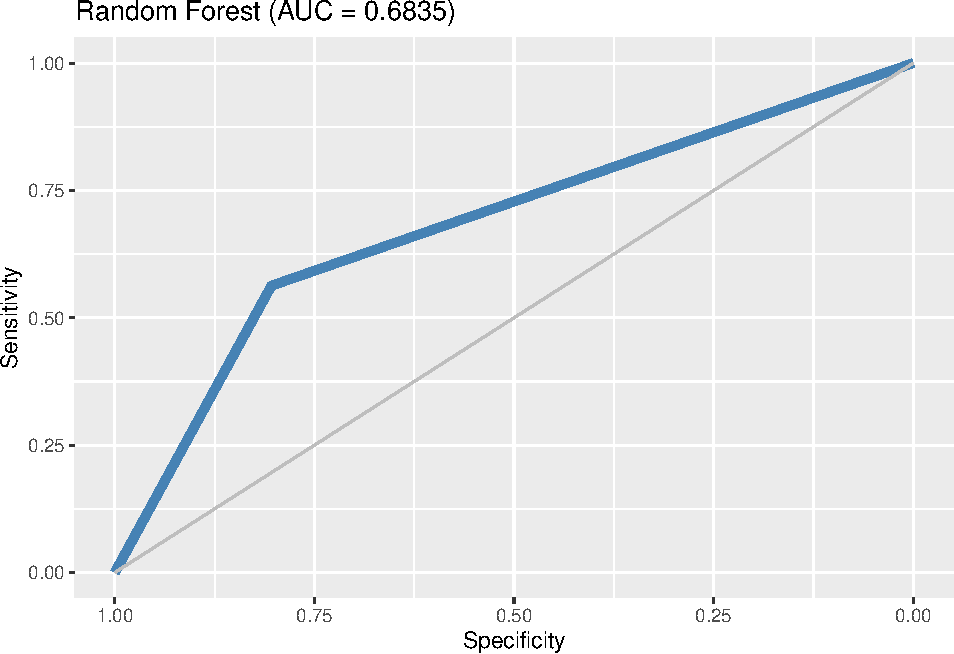
\includegraphics{06-Individual_Logistic_Models_files/figure-latex/Support Vector Machines for logistic data-1.pdf}

\begin{verbatim}
#> [1] 0.7151703

# Check for any errors
warnings()
\end{verbatim}

\subsection{XGBoost}\label{xgboost-2}

\begin{Shaded}
\begin{Highlighting}[]

\CommentTok{\# Load the library}
\FunctionTok{library}\NormalTok{(xgboost)}
\CommentTok{\#\textgreater{} }
\CommentTok{\#\textgreater{} Attaching package: \textquotesingle{}xgboost\textquotesingle{}}
\CommentTok{\#\textgreater{} The following object is masked from \textquotesingle{}package:dplyr\textquotesingle{}:}
\CommentTok{\#\textgreater{} }
\CommentTok{\#\textgreater{}     slice}
\FunctionTok{library}\NormalTok{(tidyverse)}
\FunctionTok{library}\NormalTok{(pROC)}

\CommentTok{\# Set initial values to 0}

\NormalTok{xgb\_train\_accuracy }\OtherTok{\textless{}{-}} \DecValTok{0}
\NormalTok{xgb\_test\_accuracy }\OtherTok{\textless{}{-}} \DecValTok{0}
\NormalTok{xgb\_holdout\_accuracy }\OtherTok{\textless{}{-}} \DecValTok{0}
\NormalTok{xgb\_duration }\OtherTok{\textless{}{-}} \DecValTok{0}
\NormalTok{xgb\_table\_total }\OtherTok{\textless{}{-}} \DecValTok{0}

\CommentTok{\# Create the function}

\NormalTok{xgb\_1 }\OtherTok{\textless{}{-}} \ControlFlowTok{function}\NormalTok{(data, colnum, numresamples, train\_amount, test\_amount)\{}
  
  \FunctionTok{colnames}\NormalTok{(data)[colnum] }\OtherTok{\textless{}{-}} \StringTok{"y"}
  
\NormalTok{  df }\OtherTok{\textless{}{-}}\NormalTok{ data }\SpecialCharTok{\%\textgreater{}\%}\NormalTok{ dplyr}\SpecialCharTok{::}\FunctionTok{relocate}\NormalTok{(y, }\AttributeTok{.after =} \FunctionTok{last\_col}\NormalTok{()) }\CommentTok{\# Moves the target column to the last column on the right}
  
\NormalTok{  df }\OtherTok{\textless{}{-}}\NormalTok{ df[}\FunctionTok{sample}\NormalTok{(}\DecValTok{1}\SpecialCharTok{:}\FunctionTok{nrow}\NormalTok{(df)), ] }\CommentTok{\# randomizes the rows}
  
  \CommentTok{\# Set up random resampling}
  
  \ControlFlowTok{for}\NormalTok{ (i }\ControlFlowTok{in} \DecValTok{1}\SpecialCharTok{:}\NormalTok{numresamples) \{}
    
\NormalTok{    index }\OtherTok{\textless{}{-}} \FunctionTok{sample}\NormalTok{(}\FunctionTok{c}\NormalTok{(}\DecValTok{1}\SpecialCharTok{:}\DecValTok{2}\NormalTok{), }\FunctionTok{nrow}\NormalTok{(df), }\AttributeTok{replace =} \ConstantTok{TRUE}\NormalTok{, }\AttributeTok{prob =} \FunctionTok{c}\NormalTok{(train\_amount, test\_amount))}
    
\NormalTok{    train }\OtherTok{\textless{}{-}}\NormalTok{ df[index }\SpecialCharTok{==} \DecValTok{1}\NormalTok{, ]}
\NormalTok{    test }\OtherTok{\textless{}{-}}\NormalTok{ df[index }\SpecialCharTok{==} \DecValTok{2}\NormalTok{, ]}
    
\NormalTok{    y\_train }\OtherTok{\textless{}{-}}\NormalTok{ train}\SpecialCharTok{$}\NormalTok{y}
\NormalTok{    y\_test }\OtherTok{\textless{}{-}}\NormalTok{ test}\SpecialCharTok{$}\NormalTok{y}
    
\CommentTok{\# Fit the model to the training data, make predictions on the holdout data}
\NormalTok{train\_x }\OtherTok{\textless{}{-}} \FunctionTok{data.matrix}\NormalTok{(train[, }\SpecialCharTok{{-}}\FunctionTok{ncol}\NormalTok{(train)])}
\NormalTok{train\_y }\OtherTok{\textless{}{-}}\NormalTok{ train[, }\FunctionTok{ncol}\NormalTok{(train)]}
    
\CommentTok{\# define predictor and response variables in test set}
\NormalTok{test\_x }\OtherTok{\textless{}{-}} \FunctionTok{data.matrix}\NormalTok{(test[, }\SpecialCharTok{{-}}\FunctionTok{ncol}\NormalTok{(test)])}
\NormalTok{test\_y }\OtherTok{\textless{}{-}}\NormalTok{ test[, }\FunctionTok{ncol}\NormalTok{(test)]}
    
\CommentTok{\# define final train and test sets}
\NormalTok{xgb\_train }\OtherTok{\textless{}{-}}\NormalTok{ xgboost}\SpecialCharTok{::}\FunctionTok{xgb.DMatrix}\NormalTok{(}\AttributeTok{data =}\NormalTok{ train\_x, }\AttributeTok{label =}\NormalTok{ train\_y)}
\NormalTok{xgb\_test }\OtherTok{\textless{}{-}}\NormalTok{ xgboost}\SpecialCharTok{::}\FunctionTok{xgb.DMatrix}\NormalTok{(}\AttributeTok{data =}\NormalTok{ test\_x, }\AttributeTok{label =}\NormalTok{ test\_y)}

\CommentTok{\# define watchlist}
\NormalTok{watchlist }\OtherTok{\textless{}{-}} \FunctionTok{list}\NormalTok{(}\AttributeTok{train =}\NormalTok{ xgb\_train)}
\NormalTok{watchlist\_test }\OtherTok{\textless{}{-}} \FunctionTok{list}\NormalTok{(}\AttributeTok{train =}\NormalTok{ xgb\_train, }\AttributeTok{test =}\NormalTok{ xgb\_test)}

\NormalTok{xgb\_model }\OtherTok{\textless{}{-}}\NormalTok{ xgboost}\SpecialCharTok{::}\FunctionTok{xgb.train}\NormalTok{(}\AttributeTok{data =}\NormalTok{ xgb\_train, }\AttributeTok{max.depth =} \DecValTok{3}\NormalTok{, }\AttributeTok{watchlist =}\NormalTok{ watchlist\_test, }\AttributeTok{nrounds =} \DecValTok{70}\NormalTok{)}
    
\NormalTok{xgb\_min }\OtherTok{\textless{}{-}} \FunctionTok{which.min}\NormalTok{(xgb\_model}\SpecialCharTok{$}\NormalTok{evaluation\_log}\SpecialCharTok{$}\NormalTok{validation\_rmse)}
    
\NormalTok{xgb\_train\_pred }\OtherTok{\textless{}{-}}\NormalTok{ stats}\SpecialCharTok{::}\FunctionTok{predict}\NormalTok{(}\AttributeTok{object =}\NormalTok{ xgb\_model, }\AttributeTok{newdata =}\NormalTok{ train\_x, }\AttributeTok{type =} \StringTok{"prob"}\NormalTok{)}
\NormalTok{xgb\_train\_predictions }\OtherTok{\textless{}{-}} \FunctionTok{ifelse}\NormalTok{(xgb\_train\_pred }\SpecialCharTok{\textgreater{}} \FloatTok{0.5}\NormalTok{, }\DecValTok{1}\NormalTok{, }\DecValTok{0}\NormalTok{)}
\NormalTok{xgb\_train\_table }\OtherTok{\textless{}{-}} \FunctionTok{table}\NormalTok{(xgb\_train\_predictions, y\_train)}
\NormalTok{xgb\_train\_accuracy[i] }\OtherTok{\textless{}{-}}\NormalTok{ (xgb\_train\_table[}\DecValTok{1}\NormalTok{, }\DecValTok{1}\NormalTok{] }\SpecialCharTok{+}\NormalTok{ xgb\_train\_table[}\DecValTok{2}\NormalTok{, }\DecValTok{2}\NormalTok{]) }\SpecialCharTok{/} \FunctionTok{sum}\NormalTok{(xgb\_train\_table)}
\NormalTok{xgb\_train\_accuracy\_mean }\OtherTok{\textless{}{-}} \FunctionTok{mean}\NormalTok{(xgb\_train\_accuracy)}

\NormalTok{xgb\_test\_pred }\OtherTok{\textless{}{-}}\NormalTok{ stats}\SpecialCharTok{::}\FunctionTok{predict}\NormalTok{(}\AttributeTok{object =}\NormalTok{ xgb\_model, }\AttributeTok{newdata =}\NormalTok{ test\_x, }\AttributeTok{type =} \StringTok{"prob"}\NormalTok{)}
\NormalTok{xgb\_test\_predictions }\OtherTok{\textless{}{-}} \FunctionTok{ifelse}\NormalTok{(xgb\_test\_pred }\SpecialCharTok{\textgreater{}} \FloatTok{0.5}\NormalTok{, }\DecValTok{1}\NormalTok{, }\DecValTok{0}\NormalTok{)}
\NormalTok{xgb\_test\_table }\OtherTok{\textless{}{-}} \FunctionTok{table}\NormalTok{(xgb\_test\_predictions, y\_test)}
\NormalTok{xgb\_test\_accuracy[i] }\OtherTok{\textless{}{-}}\NormalTok{ (xgb\_test\_table[}\DecValTok{1}\NormalTok{, }\DecValTok{1}\NormalTok{] }\SpecialCharTok{+}\NormalTok{ xgb\_test\_table[}\DecValTok{2}\NormalTok{, }\DecValTok{2}\NormalTok{]) }\SpecialCharTok{/} \FunctionTok{sum}\NormalTok{(xgb\_test\_table)}
\NormalTok{xgb\_test\_accuracy\_mean }\OtherTok{\textless{}{-}} \FunctionTok{mean}\NormalTok{(xgb\_test\_accuracy)}

\NormalTok{xgb\_roc\_obj }\OtherTok{\textless{}{-}}\NormalTok{ pROC}\SpecialCharTok{::}\FunctionTok{roc}\NormalTok{(}\FunctionTok{as.numeric}\NormalTok{(}\FunctionTok{c}\NormalTok{(test}\SpecialCharTok{$}\NormalTok{y)), }\FunctionTok{as.numeric}\NormalTok{(}\FunctionTok{c}\NormalTok{(xgb\_test\_pred)))}
\NormalTok{xgb\_auc }\OtherTok{\textless{}{-}} \FunctionTok{round}\NormalTok{((pROC}\SpecialCharTok{::}\FunctionTok{auc}\NormalTok{(}\FunctionTok{c}\NormalTok{(test}\SpecialCharTok{$}\NormalTok{y), }\FunctionTok{as.numeric}\NormalTok{(}\FunctionTok{c}\NormalTok{(xgb\_test\_pred)) }\SpecialCharTok{{-}} \DecValTok{1}\NormalTok{)), }\DecValTok{4}\NormalTok{)}
\FunctionTok{print}\NormalTok{(pROC}\SpecialCharTok{::}\FunctionTok{ggroc}\NormalTok{(xgb\_roc\_obj, }\AttributeTok{color =} \StringTok{"steelblue"}\NormalTok{, }\AttributeTok{size =} \DecValTok{2}\NormalTok{) }\SpecialCharTok{+}
\NormalTok{  ggplot2}\SpecialCharTok{::}\FunctionTok{ggtitle}\NormalTok{(}\FunctionTok{paste0}\NormalTok{(}\StringTok{"XGBoost "}\NormalTok{, }\StringTok{"(AUC = "}\NormalTok{, xgb\_auc, }\StringTok{")"}\NormalTok{)) }\SpecialCharTok{+}
\NormalTok{  ggplot2}\SpecialCharTok{::}\FunctionTok{labs}\NormalTok{(}\AttributeTok{x =} \StringTok{"Specificity"}\NormalTok{, }\AttributeTok{y =} \StringTok{"Sensitivity"}\NormalTok{) }\SpecialCharTok{+}
\NormalTok{  ggplot2}\SpecialCharTok{::}\FunctionTok{annotate}\NormalTok{(}\StringTok{"segment"}\NormalTok{, }\AttributeTok{x =} \DecValTok{1}\NormalTok{, }\AttributeTok{xend =} \DecValTok{0}\NormalTok{, }\AttributeTok{y =} \DecValTok{0}\NormalTok{, }\AttributeTok{yend =} \DecValTok{1}\NormalTok{, }\AttributeTok{color =} \StringTok{"grey"}\NormalTok{)}
\NormalTok{    )}
    
\FunctionTok{return}\NormalTok{(xgb\_test\_accuracy\_mean)}
    
\NormalTok{  \} }\CommentTok{\# closing brace for numresamples }
  
\NormalTok{\} }\CommentTok{\# Closing brace for the function}

\CommentTok{\# Test the function}
\FunctionTok{xgb\_1}\NormalTok{(}\AttributeTok{data =}\NormalTok{ diabetes, }\AttributeTok{colnum =} \DecValTok{9}\NormalTok{, }\AttributeTok{numresamples =} \DecValTok{5}\NormalTok{, }\AttributeTok{train\_amount =} \FloatTok{0.60}\NormalTok{, }\AttributeTok{test\_amount =} \FloatTok{0.40}\NormalTok{)}
\CommentTok{\#\textgreater{} [1]  train{-}rmse:0.441943 test{-}rmse:0.450450 }
\CommentTok{\#\textgreater{} [2]  train{-}rmse:0.404982 test{-}rmse:0.431270 }
\CommentTok{\#\textgreater{} [3]  train{-}rmse:0.378994 test{-}rmse:0.422847 }
\CommentTok{\#\textgreater{} [4]  train{-}rmse:0.363831 test{-}rmse:0.413561 }
\CommentTok{\#\textgreater{} [5]  train{-}rmse:0.352432 test{-}rmse:0.411546 }
\CommentTok{\#\textgreater{} [6]  train{-}rmse:0.343119 test{-}rmse:0.409883 }
\CommentTok{\#\textgreater{} [7]  train{-}rmse:0.335318 test{-}rmse:0.409771 }
\CommentTok{\#\textgreater{} [8]  train{-}rmse:0.328759 test{-}rmse:0.409690 }
\CommentTok{\#\textgreater{} [9]  train{-}rmse:0.321926 test{-}rmse:0.407342 }
\CommentTok{\#\textgreater{} [10] train{-}rmse:0.317653 test{-}rmse:0.404540 }
\CommentTok{\#\textgreater{} [11] train{-}rmse:0.312477 test{-}rmse:0.405154 }
\CommentTok{\#\textgreater{} [12] train{-}rmse:0.309505 test{-}rmse:0.405058 }
\CommentTok{\#\textgreater{} [13] train{-}rmse:0.305393 test{-}rmse:0.405373 }
\CommentTok{\#\textgreater{} [14] train{-}rmse:0.301884 test{-}rmse:0.407004 }
\CommentTok{\#\textgreater{} [15] train{-}rmse:0.297231 test{-}rmse:0.406674 }
\CommentTok{\#\textgreater{} [16] train{-}rmse:0.294270 test{-}rmse:0.405315 }
\CommentTok{\#\textgreater{} [17] train{-}rmse:0.289973 test{-}rmse:0.409281 }
\CommentTok{\#\textgreater{} [18] train{-}rmse:0.287709 test{-}rmse:0.408281 }
\CommentTok{\#\textgreater{} [19] train{-}rmse:0.282660 test{-}rmse:0.409966 }
\CommentTok{\#\textgreater{} [20] train{-}rmse:0.281140 test{-}rmse:0.408841 }
\CommentTok{\#\textgreater{} [21] train{-}rmse:0.279186 test{-}rmse:0.409338 }
\CommentTok{\#\textgreater{} [22] train{-}rmse:0.275709 test{-}rmse:0.411491 }
\CommentTok{\#\textgreater{} [23] train{-}rmse:0.274494 test{-}rmse:0.410780 }
\CommentTok{\#\textgreater{} [24] train{-}rmse:0.273289 test{-}rmse:0.411557 }
\CommentTok{\#\textgreater{} [25] train{-}rmse:0.270258 test{-}rmse:0.412388 }
\CommentTok{\#\textgreater{} [26] train{-}rmse:0.267258 test{-}rmse:0.415274 }
\CommentTok{\#\textgreater{} [27] train{-}rmse:0.265863 test{-}rmse:0.416823 }
\CommentTok{\#\textgreater{} [28] train{-}rmse:0.264525 test{-}rmse:0.416788 }
\CommentTok{\#\textgreater{} [29] train{-}rmse:0.261514 test{-}rmse:0.415773 }
\CommentTok{\#\textgreater{} [30] train{-}rmse:0.260036 test{-}rmse:0.416040 }
\CommentTok{\#\textgreater{} [31] train{-}rmse:0.256026 test{-}rmse:0.416875 }
\CommentTok{\#\textgreater{} [32] train{-}rmse:0.252439 test{-}rmse:0.417829 }
\CommentTok{\#\textgreater{} [33] train{-}rmse:0.247614 test{-}rmse:0.416656 }
\CommentTok{\#\textgreater{} [34] train{-}rmse:0.245022 test{-}rmse:0.416266 }
\CommentTok{\#\textgreater{} [35] train{-}rmse:0.241859 test{-}rmse:0.417454 }
\CommentTok{\#\textgreater{} [36] train{-}rmse:0.240836 test{-}rmse:0.418274 }
\CommentTok{\#\textgreater{} [37] train{-}rmse:0.237740 test{-}rmse:0.419863 }
\CommentTok{\#\textgreater{} [38] train{-}rmse:0.232971 test{-}rmse:0.419598 }
\CommentTok{\#\textgreater{} [39] train{-}rmse:0.229292 test{-}rmse:0.421749 }
\CommentTok{\#\textgreater{} [40] train{-}rmse:0.228120 test{-}rmse:0.421352 }
\CommentTok{\#\textgreater{} [41] train{-}rmse:0.227523 test{-}rmse:0.421641 }
\CommentTok{\#\textgreater{} [42] train{-}rmse:0.225333 test{-}rmse:0.419702 }
\CommentTok{\#\textgreater{} [43] train{-}rmse:0.223704 test{-}rmse:0.420101 }
\CommentTok{\#\textgreater{} [44] train{-}rmse:0.222859 test{-}rmse:0.421917 }
\CommentTok{\#\textgreater{} [45] train{-}rmse:0.221041 test{-}rmse:0.422432 }
\CommentTok{\#\textgreater{} [46] train{-}rmse:0.219120 test{-}rmse:0.423515 }
\CommentTok{\#\textgreater{} [47] train{-}rmse:0.216316 test{-}rmse:0.423367 }
\CommentTok{\#\textgreater{} [48] train{-}rmse:0.213300 test{-}rmse:0.424044 }
\CommentTok{\#\textgreater{} [49] train{-}rmse:0.211992 test{-}rmse:0.423899 }
\CommentTok{\#\textgreater{} [50] train{-}rmse:0.210670 test{-}rmse:0.424627 }
\CommentTok{\#\textgreater{} [51] train{-}rmse:0.210224 test{-}rmse:0.424881 }
\CommentTok{\#\textgreater{} [52] train{-}rmse:0.209186 test{-}rmse:0.425958 }
\CommentTok{\#\textgreater{} [53] train{-}rmse:0.206998 test{-}rmse:0.425461 }
\CommentTok{\#\textgreater{} [54] train{-}rmse:0.205883 test{-}rmse:0.426141 }
\CommentTok{\#\textgreater{} [55] train{-}rmse:0.205538 test{-}rmse:0.425693 }
\CommentTok{\#\textgreater{} [56] train{-}rmse:0.204695 test{-}rmse:0.425125 }
\CommentTok{\#\textgreater{} [57] train{-}rmse:0.204375 test{-}rmse:0.425032 }
\CommentTok{\#\textgreater{} [58] train{-}rmse:0.203478 test{-}rmse:0.425806 }
\CommentTok{\#\textgreater{} [59] train{-}rmse:0.202825 test{-}rmse:0.425452 }
\CommentTok{\#\textgreater{} [60] train{-}rmse:0.199758 test{-}rmse:0.425980 }
\CommentTok{\#\textgreater{} [61] train{-}rmse:0.196161 test{-}rmse:0.426438 }
\CommentTok{\#\textgreater{} [62] train{-}rmse:0.194400 test{-}rmse:0.425922 }
\CommentTok{\#\textgreater{} [63] train{-}rmse:0.193503 test{-}rmse:0.425974 }
\CommentTok{\#\textgreater{} [64] train{-}rmse:0.193211 test{-}rmse:0.425698 }
\CommentTok{\#\textgreater{} [65] train{-}rmse:0.192110 test{-}rmse:0.425273 }
\CommentTok{\#\textgreater{} [66] train{-}rmse:0.190284 test{-}rmse:0.426007 }
\CommentTok{\#\textgreater{} [67] train{-}rmse:0.186343 test{-}rmse:0.427452 }
\CommentTok{\#\textgreater{} [68] train{-}rmse:0.183790 test{-}rmse:0.429599 }
\CommentTok{\#\textgreater{} [69] train{-}rmse:0.181755 test{-}rmse:0.429356 }
\CommentTok{\#\textgreater{} [70] train{-}rmse:0.179123 test{-}rmse:0.429947}
\CommentTok{\#\textgreater{} Setting levels: control = 0, case = 1}
\CommentTok{\#\textgreater{} Setting direction: controls \textless{} cases}
\CommentTok{\#\textgreater{} Setting levels: control = 0, case = 1}
\CommentTok{\#\textgreater{} Setting direction: controls \textless{} cases}
\end{Highlighting}
\end{Shaded}

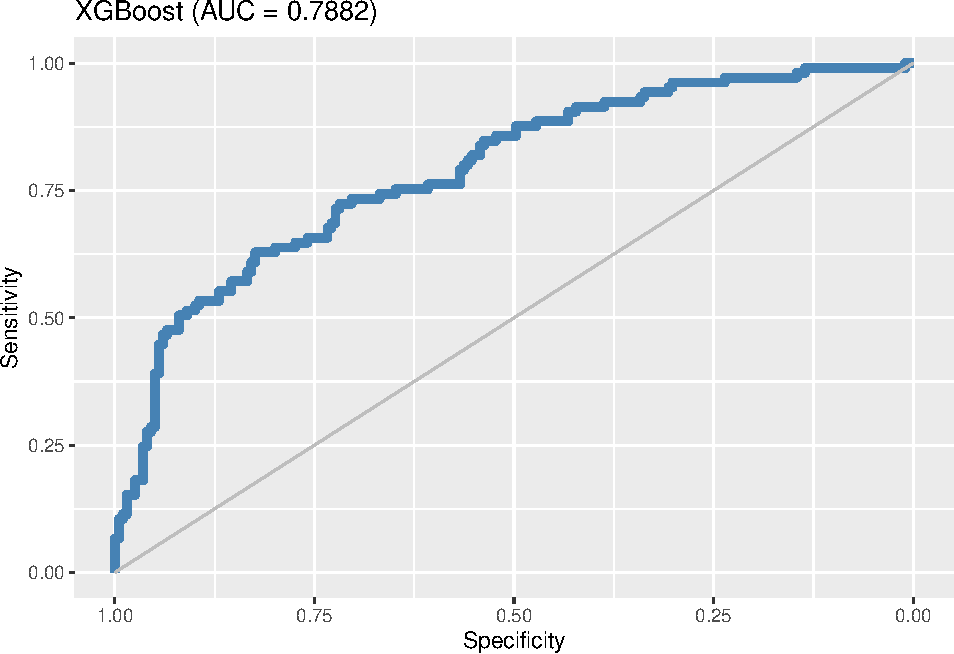
\includegraphics{06-Individual_Logistic_Models_files/figure-latex/XGBoost model for logistic data-1.pdf}

\begin{verbatim}
#> [1] 0.7565789

# Check for any errors
warnings()
\end{verbatim}

\chapter{Advice to Lebron James (and everyone who does talent analytics): Logistic ensembles}\label{advice-to-lebron-james-and-everyone-who-does-talent-analytics-logistic-ensembles}

In this section we're going to take the lessons of the previous chapter and move them into making ensembles of models. The process is extremely similar, and follows these steps:

\begin{quote}
Load the library

Set initial values to 0

Create the function

Set up random resampling

Break the data into train and test

Fit the model on the training data, make predictions and measure error on the test data

Return the results

Check for errors or warnings

Test on a different data set
\end{quote}

Logistic ensembles can be used in an extremely wide range of fields. Previously we modeled diabetes in Pima Indian women. This chapter's example will be the performance on the court of Lebron James.

Here's an image of Lebron in play.

\begin{figure}
\centering
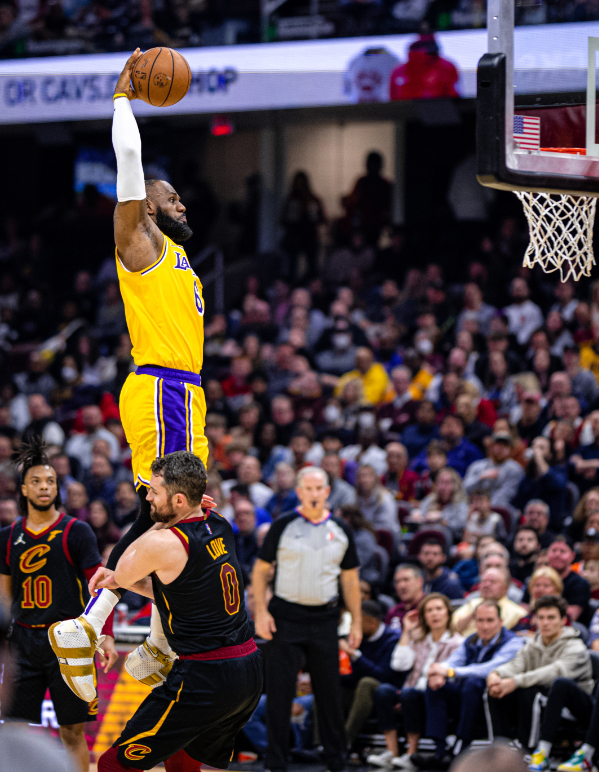
\includegraphics{_book/images/LeBron_James_small.jpg}
\caption{Lebron James}
\end{figure}

There is a LOT of data in sports and HR analytics (which are extremely similar in some ways). A lot of the data is set up as logistic data. For example, here is a data set of the performance of Lebron James. The main column of interest is ``result'', which is either 1 or 0. Thus it perfectly fits our requirements for logistic analysis.

\begin{Shaded}
\begin{Highlighting}[]

\FunctionTok{library}\NormalTok{(Ensembles)}
\CommentTok{\#\textgreater{} Loading required package: arm}
\CommentTok{\#\textgreater{} Loading required package: MASS}
\CommentTok{\#\textgreater{} Loading required package: Matrix}
\CommentTok{\#\textgreater{} Loading required package: lme4}
\CommentTok{\#\textgreater{} }
\CommentTok{\#\textgreater{} arm (Version 1.14{-}4, built: 2024{-}4{-}1)}
\CommentTok{\#\textgreater{} Working directory is /Users/russconte/Library/Mobile Documents/com\textasciitilde{}apple\textasciitilde{}CloudDocs/Documents/Machine Learning templates in R/EnsemblesBook}
\CommentTok{\#\textgreater{} Loading required package: brnn}
\CommentTok{\#\textgreater{} Loading required package: Formula}
\CommentTok{\#\textgreater{} Loading required package: truncnorm}
\CommentTok{\#\textgreater{} Loading required package: broom}
\CommentTok{\#\textgreater{} Loading required package: C50}
\CommentTok{\#\textgreater{} Loading required package: caret}
\CommentTok{\#\textgreater{} Loading required package: ggplot2}
\CommentTok{\#\textgreater{} Loading required package: lattice}
\CommentTok{\#\textgreater{} Loading required package: class}
\CommentTok{\#\textgreater{} Loading required package: corrplot}
\CommentTok{\#\textgreater{} corrplot 0.92 loaded}
\CommentTok{\#\textgreater{} }
\CommentTok{\#\textgreater{} Attaching package: \textquotesingle{}corrplot\textquotesingle{}}
\CommentTok{\#\textgreater{} The following object is masked from \textquotesingle{}package:arm\textquotesingle{}:}
\CommentTok{\#\textgreater{} }
\CommentTok{\#\textgreater{}     corrplot}
\CommentTok{\#\textgreater{} Loading required package: Cubist}
\CommentTok{\#\textgreater{} Loading required package: doParallel}
\CommentTok{\#\textgreater{} Loading required package: foreach}
\CommentTok{\#\textgreater{} Loading required package: iterators}
\CommentTok{\#\textgreater{} Loading required package: parallel}
\CommentTok{\#\textgreater{} Loading required package: dplyr}
\CommentTok{\#\textgreater{} }
\CommentTok{\#\textgreater{} Attaching package: \textquotesingle{}dplyr\textquotesingle{}}
\CommentTok{\#\textgreater{} The following object is masked from \textquotesingle{}package:MASS\textquotesingle{}:}
\CommentTok{\#\textgreater{} }
\CommentTok{\#\textgreater{}     select}
\CommentTok{\#\textgreater{} The following objects are masked from \textquotesingle{}package:stats\textquotesingle{}:}
\CommentTok{\#\textgreater{} }
\CommentTok{\#\textgreater{}     filter, lag}
\CommentTok{\#\textgreater{} The following objects are masked from \textquotesingle{}package:base\textquotesingle{}:}
\CommentTok{\#\textgreater{} }
\CommentTok{\#\textgreater{}     intersect, setdiff, setequal, union}
\CommentTok{\#\textgreater{} Loading required package: e1071}
\CommentTok{\#\textgreater{} Loading required package: fable}
\CommentTok{\#\textgreater{} Loading required package: fabletools}
\CommentTok{\#\textgreater{} Registered S3 method overwritten by \textquotesingle{}tsibble\textquotesingle{}:}
\CommentTok{\#\textgreater{}   method          from}
\CommentTok{\#\textgreater{}   format.interval inum}
\CommentTok{\#\textgreater{} }
\CommentTok{\#\textgreater{} Attaching package: \textquotesingle{}fabletools\textquotesingle{}}
\CommentTok{\#\textgreater{} The following object is masked from \textquotesingle{}package:e1071\textquotesingle{}:}
\CommentTok{\#\textgreater{} }
\CommentTok{\#\textgreater{}     interpolate}
\CommentTok{\#\textgreater{} The following objects are masked from \textquotesingle{}package:caret\textquotesingle{}:}
\CommentTok{\#\textgreater{} }
\CommentTok{\#\textgreater{}     MAE, RMSE}
\CommentTok{\#\textgreater{} The following object is masked from \textquotesingle{}package:lme4\textquotesingle{}:}
\CommentTok{\#\textgreater{} }
\CommentTok{\#\textgreater{}     refit}
\CommentTok{\#\textgreater{} Loading required package: fable.prophet}
\CommentTok{\#\textgreater{} Loading required package: Rcpp}
\CommentTok{\#\textgreater{} Loading required package: feasts}
\CommentTok{\#\textgreater{} Loading required package: gam}
\CommentTok{\#\textgreater{} Loading required package: splines}
\CommentTok{\#\textgreater{} Loaded gam 1.22{-}3}
\CommentTok{\#\textgreater{} Loading required package: gbm}
\CommentTok{\#\textgreater{} Loaded gbm 2.1.9}
\CommentTok{\#\textgreater{} This version of gbm is no longer under development. Consider transitioning to gbm3, https://github.com/gbm{-}developers/gbm3}
\CommentTok{\#\textgreater{} Loading required package: GGally}
\CommentTok{\#\textgreater{} Registered S3 method overwritten by \textquotesingle{}GGally\textquotesingle{}:}
\CommentTok{\#\textgreater{}   method from   }
\CommentTok{\#\textgreater{}   +.gg   ggplot2}
\CommentTok{\#\textgreater{} Loading required package: glmnet}
\CommentTok{\#\textgreater{} Loaded glmnet 4.1{-}8}
\CommentTok{\#\textgreater{} Loading required package: gridExtra}
\CommentTok{\#\textgreater{} }
\CommentTok{\#\textgreater{} Attaching package: \textquotesingle{}gridExtra\textquotesingle{}}
\CommentTok{\#\textgreater{} The following object is masked from \textquotesingle{}package:dplyr\textquotesingle{}:}
\CommentTok{\#\textgreater{} }
\CommentTok{\#\textgreater{}     combine}
\CommentTok{\#\textgreater{} Loading required package: gt}
\CommentTok{\#\textgreater{} Loading required package: gtExtras}
\CommentTok{\#\textgreater{} }
\CommentTok{\#\textgreater{} Attaching package: \textquotesingle{}gtExtras\textquotesingle{}}
\CommentTok{\#\textgreater{} The following object is masked from \textquotesingle{}package:MASS\textquotesingle{}:}
\CommentTok{\#\textgreater{} }
\CommentTok{\#\textgreater{}     select}
\CommentTok{\#\textgreater{} Loading required package: ipred}
\CommentTok{\#\textgreater{} Loading required package: kernlab}
\CommentTok{\#\textgreater{} }
\CommentTok{\#\textgreater{} Attaching package: \textquotesingle{}kernlab\textquotesingle{}}
\CommentTok{\#\textgreater{} The following object is masked from \textquotesingle{}package:ggplot2\textquotesingle{}:}
\CommentTok{\#\textgreater{} }
\CommentTok{\#\textgreater{}     alpha}
\CommentTok{\#\textgreater{} Loading required package: klaR}
\CommentTok{\#\textgreater{} Loading required package: leaps}
\CommentTok{\#\textgreater{} Loading required package: MachineShop}
\CommentTok{\#\textgreater{} }
\CommentTok{\#\textgreater{} Attaching package: \textquotesingle{}MachineShop\textquotesingle{}}
\CommentTok{\#\textgreater{} The following objects are masked from \textquotesingle{}package:fabletools\textquotesingle{}:}
\CommentTok{\#\textgreater{} }
\CommentTok{\#\textgreater{}     accuracy, response}
\CommentTok{\#\textgreater{} The following objects are masked from \textquotesingle{}package:caret\textquotesingle{}:}
\CommentTok{\#\textgreater{} }
\CommentTok{\#\textgreater{}     calibration, lift, precision, recall, rfe,}
\CommentTok{\#\textgreater{}     sensitivity, specificity}
\CommentTok{\#\textgreater{} The following object is masked from \textquotesingle{}package:stats\textquotesingle{}:}
\CommentTok{\#\textgreater{} }
\CommentTok{\#\textgreater{}     ppr}
\CommentTok{\#\textgreater{} Loading required package: magrittr}
\CommentTok{\#\textgreater{} Loading required package: mda}
\CommentTok{\#\textgreater{} Loaded mda 0.5{-}4}
\CommentTok{\#\textgreater{} }
\CommentTok{\#\textgreater{} Attaching package: \textquotesingle{}mda\textquotesingle{}}
\CommentTok{\#\textgreater{} The following object is masked from \textquotesingle{}package:MachineShop\textquotesingle{}:}
\CommentTok{\#\textgreater{} }
\CommentTok{\#\textgreater{}     confusion}
\CommentTok{\#\textgreater{} Loading required package: Metrics}
\CommentTok{\#\textgreater{} }
\CommentTok{\#\textgreater{} Attaching package: \textquotesingle{}Metrics\textquotesingle{}}
\CommentTok{\#\textgreater{} The following objects are masked from \textquotesingle{}package:MachineShop\textquotesingle{}:}
\CommentTok{\#\textgreater{} }
\CommentTok{\#\textgreater{}     accuracy, auc, mae, mse, msle, precision, recall,}
\CommentTok{\#\textgreater{}     rmse, rmsle}
\CommentTok{\#\textgreater{} The following object is masked from \textquotesingle{}package:fabletools\textquotesingle{}:}
\CommentTok{\#\textgreater{} }
\CommentTok{\#\textgreater{}     accuracy}
\CommentTok{\#\textgreater{} The following objects are masked from \textquotesingle{}package:caret\textquotesingle{}:}
\CommentTok{\#\textgreater{} }
\CommentTok{\#\textgreater{}     precision, recall}
\CommentTok{\#\textgreater{} Loading required package: neuralnet}
\CommentTok{\#\textgreater{} }
\CommentTok{\#\textgreater{} Attaching package: \textquotesingle{}neuralnet\textquotesingle{}}
\CommentTok{\#\textgreater{} The following object is masked from \textquotesingle{}package:dplyr\textquotesingle{}:}
\CommentTok{\#\textgreater{} }
\CommentTok{\#\textgreater{}     compute}
\CommentTok{\#\textgreater{} Loading required package: pls}
\CommentTok{\#\textgreater{} }
\CommentTok{\#\textgreater{} Attaching package: \textquotesingle{}pls\textquotesingle{}}
\CommentTok{\#\textgreater{} The following object is masked from \textquotesingle{}package:corrplot\textquotesingle{}:}
\CommentTok{\#\textgreater{} }
\CommentTok{\#\textgreater{}     corrplot}
\CommentTok{\#\textgreater{} The following object is masked from \textquotesingle{}package:caret\textquotesingle{}:}
\CommentTok{\#\textgreater{} }
\CommentTok{\#\textgreater{}     R2}
\CommentTok{\#\textgreater{} The following objects are masked from \textquotesingle{}package:arm\textquotesingle{}:}
\CommentTok{\#\textgreater{} }
\CommentTok{\#\textgreater{}     coefplot, corrplot}
\CommentTok{\#\textgreater{} The following object is masked from \textquotesingle{}package:stats\textquotesingle{}:}
\CommentTok{\#\textgreater{} }
\CommentTok{\#\textgreater{}     loadings}
\CommentTok{\#\textgreater{} Loading required package: pROC}
\CommentTok{\#\textgreater{} Type \textquotesingle{}citation("pROC")\textquotesingle{} for a citation.}
\CommentTok{\#\textgreater{} }
\CommentTok{\#\textgreater{} Attaching package: \textquotesingle{}pROC\textquotesingle{}}
\CommentTok{\#\textgreater{} The following object is masked from \textquotesingle{}package:Metrics\textquotesingle{}:}
\CommentTok{\#\textgreater{} }
\CommentTok{\#\textgreater{}     auc}
\CommentTok{\#\textgreater{} The following object is masked from \textquotesingle{}package:MachineShop\textquotesingle{}:}
\CommentTok{\#\textgreater{} }
\CommentTok{\#\textgreater{}     auc}
\CommentTok{\#\textgreater{} The following objects are masked from \textquotesingle{}package:stats\textquotesingle{}:}
\CommentTok{\#\textgreater{} }
\CommentTok{\#\textgreater{}     cov, smooth, var}
\CommentTok{\#\textgreater{} Loading required package: purrr}
\CommentTok{\#\textgreater{} }
\CommentTok{\#\textgreater{} Attaching package: \textquotesingle{}purrr\textquotesingle{}}
\CommentTok{\#\textgreater{} The following object is masked from \textquotesingle{}package:magrittr\textquotesingle{}:}
\CommentTok{\#\textgreater{} }
\CommentTok{\#\textgreater{}     set\_names}
\CommentTok{\#\textgreater{} The following object is masked from \textquotesingle{}package:MachineShop\textquotesingle{}:}
\CommentTok{\#\textgreater{} }
\CommentTok{\#\textgreater{}     lift}
\CommentTok{\#\textgreater{} The following object is masked from \textquotesingle{}package:kernlab\textquotesingle{}:}
\CommentTok{\#\textgreater{} }
\CommentTok{\#\textgreater{}     cross}
\CommentTok{\#\textgreater{} The following objects are masked from \textquotesingle{}package:foreach\textquotesingle{}:}
\CommentTok{\#\textgreater{} }
\CommentTok{\#\textgreater{}     accumulate, when}
\CommentTok{\#\textgreater{} The following object is masked from \textquotesingle{}package:caret\textquotesingle{}:}
\CommentTok{\#\textgreater{} }
\CommentTok{\#\textgreater{}     lift}
\CommentTok{\#\textgreater{} Loading required package: randomForest}
\CommentTok{\#\textgreater{} randomForest 4.7{-}1.1}
\CommentTok{\#\textgreater{} Type rfNews() to see new features/changes/bug fixes.}
\CommentTok{\#\textgreater{} }
\CommentTok{\#\textgreater{} Attaching package: \textquotesingle{}randomForest\textquotesingle{}}
\CommentTok{\#\textgreater{} The following object is masked from \textquotesingle{}package:gridExtra\textquotesingle{}:}
\CommentTok{\#\textgreater{} }
\CommentTok{\#\textgreater{}     combine}
\CommentTok{\#\textgreater{} The following object is masked from \textquotesingle{}package:dplyr\textquotesingle{}:}
\CommentTok{\#\textgreater{} }
\CommentTok{\#\textgreater{}     combine}
\CommentTok{\#\textgreater{} The following object is masked from \textquotesingle{}package:ggplot2\textquotesingle{}:}
\CommentTok{\#\textgreater{} }
\CommentTok{\#\textgreater{}     margin}
\CommentTok{\#\textgreater{} Loading required package: reactable}
\CommentTok{\#\textgreater{} Loading required package: reactablefmtr}
\CommentTok{\#\textgreater{} }
\CommentTok{\#\textgreater{} Attaching package: \textquotesingle{}reactablefmtr\textquotesingle{}}
\CommentTok{\#\textgreater{} The following object is masked from \textquotesingle{}package:randomForest\textquotesingle{}:}
\CommentTok{\#\textgreater{} }
\CommentTok{\#\textgreater{}     margin}
\CommentTok{\#\textgreater{} The following objects are masked from \textquotesingle{}package:gt\textquotesingle{}:}
\CommentTok{\#\textgreater{} }
\CommentTok{\#\textgreater{}     google\_font, html}
\CommentTok{\#\textgreater{} The following object is masked from \textquotesingle{}package:ggplot2\textquotesingle{}:}
\CommentTok{\#\textgreater{} }
\CommentTok{\#\textgreater{}     margin}
\CommentTok{\#\textgreater{} Loading required package: readr}
\CommentTok{\#\textgreater{} Loading required package: rpart}
\CommentTok{\#\textgreater{} Loading required package: scales}
\CommentTok{\#\textgreater{} }
\CommentTok{\#\textgreater{} Attaching package: \textquotesingle{}scales\textquotesingle{}}
\CommentTok{\#\textgreater{} The following object is masked from \textquotesingle{}package:readr\textquotesingle{}:}
\CommentTok{\#\textgreater{} }
\CommentTok{\#\textgreater{}     col\_factor}
\CommentTok{\#\textgreater{} The following object is masked from \textquotesingle{}package:purrr\textquotesingle{}:}
\CommentTok{\#\textgreater{} }
\CommentTok{\#\textgreater{}     discard}
\CommentTok{\#\textgreater{} The following object is masked from \textquotesingle{}package:kernlab\textquotesingle{}:}
\CommentTok{\#\textgreater{} }
\CommentTok{\#\textgreater{}     alpha}
\CommentTok{\#\textgreater{} The following object is masked from \textquotesingle{}package:arm\textquotesingle{}:}
\CommentTok{\#\textgreater{} }
\CommentTok{\#\textgreater{}     rescale}
\CommentTok{\#\textgreater{} Loading required package: tibble}
\CommentTok{\#\textgreater{} Loading required package: tidyr}
\CommentTok{\#\textgreater{} }
\CommentTok{\#\textgreater{} Attaching package: \textquotesingle{}tidyr\textquotesingle{}}
\CommentTok{\#\textgreater{} The following object is masked from \textquotesingle{}package:magrittr\textquotesingle{}:}
\CommentTok{\#\textgreater{} }
\CommentTok{\#\textgreater{}     extract}
\CommentTok{\#\textgreater{} The following objects are masked from \textquotesingle{}package:Matrix\textquotesingle{}:}
\CommentTok{\#\textgreater{} }
\CommentTok{\#\textgreater{}     expand, pack, unpack}
\CommentTok{\#\textgreater{} Loading required package: tree}
\CommentTok{\#\textgreater{} Loading required package: tsibble}
\CommentTok{\#\textgreater{} }
\CommentTok{\#\textgreater{} Attaching package: \textquotesingle{}tsibble\textquotesingle{}}
\CommentTok{\#\textgreater{} The following objects are masked from \textquotesingle{}package:base\textquotesingle{}:}
\CommentTok{\#\textgreater{} }
\CommentTok{\#\textgreater{}     intersect, setdiff, union}
\CommentTok{\#\textgreater{} Loading required package: xgboost}
\CommentTok{\#\textgreater{} }
\CommentTok{\#\textgreater{} Attaching package: \textquotesingle{}xgboost\textquotesingle{}}
\CommentTok{\#\textgreater{} The following object is masked from \textquotesingle{}package:dplyr\textquotesingle{}:}
\CommentTok{\#\textgreater{} }
\CommentTok{\#\textgreater{}     slice}
\FunctionTok{head}\NormalTok{(lebron, }\AttributeTok{n =} \DecValTok{20}\NormalTok{)}
\CommentTok{\#\textgreater{}    top left  date qtr time\_remaining result shot\_type}
\CommentTok{\#\textgreater{} 1  310  203 19283   2            566      0         3}
\CommentTok{\#\textgreater{} 2  213  259 19283   2            518      0         2}
\CommentTok{\#\textgreater{} 3  143  171 19283   2            490      0         2}
\CommentTok{\#\textgreater{} 4   68  215 19283   2            324      1         2}
\CommentTok{\#\textgreater{} 5   66  470 19283   2             62      0         3}
\CommentTok{\#\textgreater{} 6   63  239 19283   4            690      1         2}
\CommentTok{\#\textgreater{} 7  230   54 19283   4            630      0         3}
\CommentTok{\#\textgreater{} 8   53  224 19283   4            605      1         2}
\CommentTok{\#\textgreater{} 9  241   67 19283   4            570      0         3}
\CommentTok{\#\textgreater{} 10 273  113 19283   4            535      0         3}
\CommentTok{\#\textgreater{} 11  62  224 19283   4            426      0         2}
\CommentTok{\#\textgreater{} 12  63  249 19283   4            233      1         2}
\CommentTok{\#\textgreater{} 13 103  236 19283   4            154      0         2}
\CommentTok{\#\textgreater{} 14  54  249 19283   4            108      1         2}
\CommentTok{\#\textgreater{} 15  53  240 19283   4             58      0         2}
\CommentTok{\#\textgreater{} 16 230   71 19283   5            649      1         3}
\CommentTok{\#\textgreater{} 17 231  358 19283   5            540      0         2}
\CommentTok{\#\textgreater{} 18  61  240 19283   5            524      1         2}
\CommentTok{\#\textgreater{} 19  59  235 19283   5             71      1         2}
\CommentTok{\#\textgreater{} 20 299  188 19283   5              6      1         3}
\CommentTok{\#\textgreater{}    distance\_ft lead lebron\_team\_score opponent\_team\_score}
\CommentTok{\#\textgreater{} 1           26    0                 2                   2}
\CommentTok{\#\textgreater{} 2           16    0                 4                   5}
\CommentTok{\#\textgreater{} 3           11    0                 4                   7}
\CommentTok{\#\textgreater{} 4            3    0                12                  19}
\CommentTok{\#\textgreater{} 5           23    0                22                  23}
\CommentTok{\#\textgreater{} 6            1    0                24                  25}
\CommentTok{\#\textgreater{} 7           26    0                24                  27}
\CommentTok{\#\textgreater{} 8            2    0                26                  27}
\CommentTok{\#\textgreater{} 9           26    0                26                  29}
\CommentTok{\#\textgreater{} 10          25    0                26                  32}
\CommentTok{\#\textgreater{} 11           2    0                31                  39}
\CommentTok{\#\textgreater{} 12           1    0                39                  49}
\CommentTok{\#\textgreater{} 13           5    0                39                  51}
\CommentTok{\#\textgreater{} 14           1    0                44                  53}
\CommentTok{\#\textgreater{} 15           0    0                46                  55}
\CommentTok{\#\textgreater{} 16          25    0                58                  63}
\CommentTok{\#\textgreater{} 17          21    0                60                  70}
\CommentTok{\#\textgreater{} 18           1    0                62                  70}
\CommentTok{\#\textgreater{} 19           1    0                68                  91}
\CommentTok{\#\textgreater{} 20          25    0                71                  91}
\CommentTok{\#\textgreater{}    opponent}
\CommentTok{\#\textgreater{} 1         9}
\CommentTok{\#\textgreater{} 2         9}
\CommentTok{\#\textgreater{} 3         9}
\CommentTok{\#\textgreater{} 4         9}
\CommentTok{\#\textgreater{} 5         9}
\CommentTok{\#\textgreater{} 6         9}
\CommentTok{\#\textgreater{} 7         9}
\CommentTok{\#\textgreater{} 8         9}
\CommentTok{\#\textgreater{} 9         9}
\CommentTok{\#\textgreater{} 10        9}
\CommentTok{\#\textgreater{} 11        9}
\CommentTok{\#\textgreater{} 12        9}
\CommentTok{\#\textgreater{} 13        9}
\CommentTok{\#\textgreater{} 14        9}
\CommentTok{\#\textgreater{} 15        9}
\CommentTok{\#\textgreater{} 16        9}
\CommentTok{\#\textgreater{} 17        9}
\CommentTok{\#\textgreater{} 18        9}
\CommentTok{\#\textgreater{} 19        9}
\CommentTok{\#\textgreater{} 20        9}
\end{Highlighting}
\end{Shaded}

Let's look at the structure of the data:

\begin{Shaded}
\begin{Highlighting}[]
\NormalTok{lebron }\OtherTok{\textless{}{-}}\NormalTok{ Ensembles}\SpecialCharTok{::}\NormalTok{lebron}
\FunctionTok{str}\NormalTok{(Ensembles}\SpecialCharTok{::}\NormalTok{lebron)}
\CommentTok{\#\textgreater{} \textquotesingle{}data.frame\textquotesingle{}:    1533 obs. of  12 variables:}
\CommentTok{\#\textgreater{}  $ top                : int  310 213 143 68 66 63 230 53 241 273 ...}
\CommentTok{\#\textgreater{}  $ left               : int  203 259 171 215 470 239 54 224 67 113 ...}
\CommentTok{\#\textgreater{}  $ date               : num  19283 19283 19283 19283 19283 ...}
\CommentTok{\#\textgreater{}  $ qtr                : num  2 2 2 2 2 4 4 4 4 4 ...}
\CommentTok{\#\textgreater{}  $ time\_remaining     : num  566 518 490 324 62 690 630 605 570 535 ...}
\CommentTok{\#\textgreater{}  $ result             : num  0 0 0 1 0 1 0 1 0 0 ...}
\CommentTok{\#\textgreater{}  $ shot\_type          : int  3 2 2 2 3 2 3 2 3 3 ...}
\CommentTok{\#\textgreater{}  $ distance\_ft        : int  26 16 11 3 23 1 26 2 26 25 ...}
\CommentTok{\#\textgreater{}  $ lead               : num  0 0 0 0 0 0 0 0 0 0 ...}
\CommentTok{\#\textgreater{}  $ lebron\_team\_score  : int  2 4 4 12 22 24 24 26 26 26 ...}
\CommentTok{\#\textgreater{}  $ opponent\_team\_score: int  2 5 7 19 23 25 27 27 29 32 ...}
\CommentTok{\#\textgreater{}  $ opponent           : num  9 9 9 9 9 9 9 9 9 9 ...}
\end{Highlighting}
\end{Shaded}

We see that all of these are numbers. It might be easier if ``qtr'' and ``opponent'' were changed to factors, so we'll do that first.

\begin{Shaded}
\begin{Highlighting}[]

\NormalTok{lebron}\SpecialCharTok{$}\NormalTok{qtr }\OtherTok{\textless{}{-}} \FunctionTok{as.factor}\NormalTok{(lebron}\SpecialCharTok{$}\NormalTok{qtr)}
\NormalTok{lebron}\SpecialCharTok{$}\NormalTok{opponent }\OtherTok{\textless{}{-}} \FunctionTok{as.factor}\NormalTok{(lebron}\SpecialCharTok{$}\NormalTok{opponent)}
\end{Highlighting}
\end{Shaded}

Now we're ready to create an ensemble of models to make predictions about Lebron's future performance. The new skill in this chapter will be saving all trained models to the Environment. This will allow us to look at the trained models, and use them to make the strongest evidence based recommendations.

We will use the following individual models and ensemble of models:

Individual models:

AdaBoost

BayesGLM

C50

Cubist

Generalized Linear Models (GLM)

Random Forest

XGBoost

We will make an ensemble of the predictions from those five models, and then use that ensemble to model predictions for Lebron's performance.

We will also show the ROC curves for each of the results, and save all the trained models at the end.

\begin{Shaded}
\begin{Highlighting}[]

\CommentTok{\# Load libraries {-} note these will work with individual and ensemble models}
\FunctionTok{library}\NormalTok{(arm) }\CommentTok{\# to use with BayesGLM}
\FunctionTok{library}\NormalTok{(C50) }\CommentTok{\# To use with C50}
\FunctionTok{library}\NormalTok{(Cubist) }\CommentTok{\# To use with Cubist modeling}
\FunctionTok{library}\NormalTok{(MachineShop)}\CommentTok{\# To use with ADABoost}
\FunctionTok{library}\NormalTok{(randomForest) }\CommentTok{\# Random Forest models}
\FunctionTok{library}\NormalTok{(tidyverse) }\CommentTok{\# My favorite tool for data science!}
\CommentTok{\#\textgreater{} {-}{-} Attaching core tidyverse packages {-}{-}{-}{-} tidyverse 2.0.0 {-}{-}}
\CommentTok{\#\textgreater{} v forcats   1.0.0     v stringr   1.5.1}
\CommentTok{\#\textgreater{} v lubridate 1.9.3     }
\CommentTok{\#\textgreater{} {-}{-} Conflicts {-}{-}{-}{-}{-}{-}{-}{-}{-}{-}{-}{-}{-}{-}{-}{-}{-}{-}{-}{-}{-}{-} tidyverse\_conflicts() {-}{-}}
\CommentTok{\#\textgreater{} x purrr::accumulate()     masks foreach::accumulate()}
\CommentTok{\#\textgreater{} x scales::alpha()         masks kernlab::alpha(), ggplot2::alpha()}
\CommentTok{\#\textgreater{} x scales::col\_factor()    masks readr::col\_factor()}
\CommentTok{\#\textgreater{} x randomForest::combine() masks gridExtra::combine(), dplyr::combine()}
\CommentTok{\#\textgreater{} x neuralnet::compute()    masks dplyr::compute()}
\CommentTok{\#\textgreater{} x purrr::cross()          masks kernlab::cross()}
\CommentTok{\#\textgreater{} x scales::discard()       masks purrr::discard()}
\CommentTok{\#\textgreater{} x tidyr::expand()         masks Matrix::expand()}
\CommentTok{\#\textgreater{} x tidyr::extract()        masks magrittr::extract()}
\CommentTok{\#\textgreater{} x dplyr::filter()         masks stats::filter()}
\CommentTok{\#\textgreater{} x lubridate::interval()   masks tsibble::interval()}
\CommentTok{\#\textgreater{} x dplyr::lag()            masks stats::lag()}
\CommentTok{\#\textgreater{} x purrr::lift()           masks MachineShop::lift(), caret::lift()}
\CommentTok{\#\textgreater{} x reactablefmtr::margin() masks randomForest::margin(), ggplot2::margin()}
\CommentTok{\#\textgreater{} x tidyr::pack()           masks Matrix::pack()}
\CommentTok{\#\textgreater{} x gtExtras::select()      masks dplyr::select(), MASS::select()}
\CommentTok{\#\textgreater{} x purrr::set\_names()      masks magrittr::set\_names()}
\CommentTok{\#\textgreater{} x xgboost::slice()        masks dplyr::slice()}
\CommentTok{\#\textgreater{} x tidyr::unpack()         masks Matrix::unpack()}
\CommentTok{\#\textgreater{} x purrr::when()           masks foreach::when()}
\CommentTok{\#\textgreater{} i Use the conflicted package (\textless{}http://conflicted.r{-}lib.org/\textgreater{}) to force all conflicts to become errors}
\FunctionTok{library}\NormalTok{(pROC) }\CommentTok{\# To print ROC curves}

\CommentTok{\# Set initial values to 0}
\NormalTok{adaboost\_train\_accuracy }\OtherTok{\textless{}{-}} \DecValTok{0}
\NormalTok{adaboost\_test\_accuracy }\OtherTok{\textless{}{-}} \DecValTok{0}
\NormalTok{adaboost\_holdout\_accuracy }\OtherTok{\textless{}{-}} \DecValTok{0}
\NormalTok{adaboost\_duration }\OtherTok{\textless{}{-}} \DecValTok{0}
\NormalTok{adaboost\_table\_total }\OtherTok{\textless{}{-}} \DecValTok{0}

\NormalTok{bayesglm\_train\_accuracy }\OtherTok{\textless{}{-}} \DecValTok{0}
\NormalTok{bayesglm\_test\_accuracy }\OtherTok{\textless{}{-}} \DecValTok{0}
\NormalTok{bayesglm\_holdout\_accuracy }\OtherTok{\textless{}{-}} \DecValTok{0}
\NormalTok{bayesglm\_duration }\OtherTok{\textless{}{-}} \DecValTok{0}
\NormalTok{bayesglm\_table\_total }\OtherTok{\textless{}{-}} \DecValTok{0}

\NormalTok{C50\_train\_accuracy }\OtherTok{\textless{}{-}} \DecValTok{0}
\NormalTok{C50\_test\_accuracy }\OtherTok{\textless{}{-}} \DecValTok{0}
\NormalTok{C50\_holdout\_accuracy }\OtherTok{\textless{}{-}} \DecValTok{0}
\NormalTok{C50\_duration }\OtherTok{\textless{}{-}} \DecValTok{0}
\NormalTok{C50\_table\_total }\OtherTok{\textless{}{-}} \DecValTok{0}

\NormalTok{cubist\_train\_accuracy }\OtherTok{\textless{}{-}} \DecValTok{0}
\NormalTok{cubist\_test\_accuracy }\OtherTok{\textless{}{-}} \DecValTok{0}
\NormalTok{cubist\_holdout\_accuracy }\OtherTok{\textless{}{-}} \DecValTok{0}
\NormalTok{cubist\_duration }\OtherTok{\textless{}{-}} \DecValTok{0}
\NormalTok{cubist\_table\_total }\OtherTok{\textless{}{-}} \DecValTok{0}

\NormalTok{rf\_train\_accuracy }\OtherTok{\textless{}{-}} \DecValTok{0}
\NormalTok{rf\_test\_accuracy }\OtherTok{\textless{}{-}} \DecValTok{0}
\NormalTok{rf\_holdout\_accuracy }\OtherTok{\textless{}{-}} \DecValTok{0}
\NormalTok{rf\_duration }\OtherTok{\textless{}{-}} \DecValTok{0}
\NormalTok{rf\_table\_total }\OtherTok{\textless{}{-}} \DecValTok{0}

\NormalTok{xgb\_train\_accuracy }\OtherTok{\textless{}{-}} \DecValTok{0}
\NormalTok{xgb\_test\_accuracy }\OtherTok{\textless{}{-}} \DecValTok{0}
\NormalTok{xgb\_holdout\_accuracy }\OtherTok{\textless{}{-}} \DecValTok{0}
\NormalTok{xgb\_duration }\OtherTok{\textless{}{-}} \DecValTok{0}
\NormalTok{xgb\_table\_total }\OtherTok{\textless{}{-}} \DecValTok{0}


\NormalTok{ensemble\_adaboost\_train\_accuracy }\OtherTok{\textless{}{-}} \DecValTok{0}
\NormalTok{ensemble\_adaboost\_test\_accuracy }\OtherTok{\textless{}{-}} \DecValTok{0}
\NormalTok{ensemble\_adaboost\_holdout\_accuracy }\OtherTok{\textless{}{-}} \DecValTok{0}
\NormalTok{ensemble\_adaboost\_duration }\OtherTok{\textless{}{-}} \DecValTok{0}
\NormalTok{ensemble\_adaboost\_table\_total }\OtherTok{\textless{}{-}} \DecValTok{0}
\NormalTok{ensemble\_adaboost\_train\_pred }\OtherTok{\textless{}{-}} \DecValTok{0}

\NormalTok{ensemble\_bayesglm\_train\_accuracy }\OtherTok{\textless{}{-}} \DecValTok{0}
\NormalTok{ensemble\_bayesglm\_test\_accuracy }\OtherTok{\textless{}{-}} \DecValTok{0}
\NormalTok{ensemble\_bayesglm\_holdout\_accuracy }\OtherTok{\textless{}{-}} \DecValTok{0}
\NormalTok{ensemble\_bayesglm\_duration }\OtherTok{\textless{}{-}} \DecValTok{0}
\NormalTok{ensemble\_bayesglm\_table\_total }\OtherTok{\textless{}{-}} \DecValTok{0}

\NormalTok{ensemble\_C50\_train\_accuracy }\OtherTok{\textless{}{-}} \DecValTok{0}
\NormalTok{ensemble\_C50\_test\_accuracy }\OtherTok{\textless{}{-}} \DecValTok{0}
\NormalTok{ensemble\_C50\_holdout\_accuracy }\OtherTok{\textless{}{-}} \DecValTok{0}
\NormalTok{ensemble\_C50\_duration }\OtherTok{\textless{}{-}} \DecValTok{0}
\NormalTok{ensemble\_C50\_table\_total }\OtherTok{\textless{}{-}} \DecValTok{0}

\NormalTok{ensemble\_rf\_train\_accuracy }\OtherTok{\textless{}{-}} \DecValTok{0}
\NormalTok{ensemble\_rf\_test\_accuracy }\OtherTok{\textless{}{-}} \DecValTok{0}
\NormalTok{ensemble\_rf\_holdout\_accuracy }\OtherTok{\textless{}{-}} \DecValTok{0}
\NormalTok{ensemble\_rf\_duration }\OtherTok{\textless{}{-}} \DecValTok{0}
\NormalTok{ensemble\_rf\_table\_total }\OtherTok{\textless{}{-}} \DecValTok{0}

\NormalTok{ensemble\_xgb\_train\_accuracy }\OtherTok{\textless{}{-}} \DecValTok{0}
\NormalTok{ensemble\_xgb\_test\_accuracy }\OtherTok{\textless{}{-}} \DecValTok{0}
\NormalTok{ensemble\_xgb\_holdout\_accuracy }\OtherTok{\textless{}{-}} \DecValTok{0}
\NormalTok{ensemble\_xgb\_duration }\OtherTok{\textless{}{-}} \DecValTok{0}
\NormalTok{ensemble\_xgb\_table\_total }\OtherTok{\textless{}{-}} \DecValTok{0}

\CommentTok{\# Create the function}

\NormalTok{logistic\_1 }\OtherTok{\textless{}{-}} \ControlFlowTok{function}\NormalTok{(data, colnum, numresamples, train\_amount, test\_amount)\{}
\FunctionTok{colnames}\NormalTok{(data)[colnum] }\OtherTok{\textless{}{-}} \StringTok{"y"}
  
\NormalTok{df }\OtherTok{\textless{}{-}}\NormalTok{ data }\SpecialCharTok{\%\textgreater{}\%}\NormalTok{ dplyr}\SpecialCharTok{::}\FunctionTok{relocate}\NormalTok{(y, }\AttributeTok{.after =} \FunctionTok{last\_col}\NormalTok{()) }\CommentTok{\# Moves the target column to the last column on the right}
  
\NormalTok{df }\OtherTok{\textless{}{-}}\NormalTok{ df[}\FunctionTok{sample}\NormalTok{(}\DecValTok{1}\SpecialCharTok{:}\FunctionTok{nrow}\NormalTok{(df)), ] }\CommentTok{\# randomizes the rows}
  
\CommentTok{\# Set up random resampling}
  
\ControlFlowTok{for}\NormalTok{ (i }\ControlFlowTok{in} \DecValTok{1}\SpecialCharTok{:}\NormalTok{numresamples) \{}
    
\NormalTok{index }\OtherTok{\textless{}{-}} \FunctionTok{sample}\NormalTok{(}\FunctionTok{c}\NormalTok{(}\DecValTok{1}\SpecialCharTok{:}\DecValTok{2}\NormalTok{), }\FunctionTok{nrow}\NormalTok{(df), }\AttributeTok{replace =} \ConstantTok{TRUE}\NormalTok{, }\AttributeTok{prob =} \FunctionTok{c}\NormalTok{(train\_amount, test\_amount))}
    
\NormalTok{train }\OtherTok{\textless{}{-}}\NormalTok{ df[index }\SpecialCharTok{==} \DecValTok{1}\NormalTok{, ]}
\NormalTok{test }\OtherTok{\textless{}{-}}\NormalTok{ df[index }\SpecialCharTok{==} \DecValTok{2}\NormalTok{, ]}
    
\NormalTok{y\_train }\OtherTok{\textless{}{-}}\NormalTok{ train}\SpecialCharTok{$}\NormalTok{y}
\NormalTok{y\_test }\OtherTok{\textless{}{-}}\NormalTok{ test}\SpecialCharTok{$}\NormalTok{y}
  
  
\CommentTok{\# ADABoost model}
\NormalTok{adaboost\_train\_fit }\OtherTok{\textless{}{-}}\NormalTok{ MachineShop}\SpecialCharTok{::}\FunctionTok{fit}\NormalTok{(}\AttributeTok{formula =} \FunctionTok{as.factor}\NormalTok{(y) }\SpecialCharTok{\textasciitilde{}}\NormalTok{ ., }\AttributeTok{data =}\NormalTok{ train, }\AttributeTok{model =} \StringTok{"AdaBoostModel"}\NormalTok{)}

\NormalTok{adaboost\_train\_pred }\OtherTok{\textless{}{-}}\NormalTok{ stats}\SpecialCharTok{::}\FunctionTok{predict}\NormalTok{(adaboost\_train\_fit, train, }\AttributeTok{type =} \StringTok{"prob"}\NormalTok{)}
\NormalTok{adaboost\_train\_predictions }\OtherTok{\textless{}{-}} \FunctionTok{ifelse}\NormalTok{(adaboost\_train\_pred }\SpecialCharTok{\textgreater{}} \FloatTok{0.5}\NormalTok{, }\DecValTok{1}\NormalTok{, }\DecValTok{0}\NormalTok{)}
\NormalTok{adaboost\_train\_table }\OtherTok{\textless{}{-}} \FunctionTok{table}\NormalTok{(adaboost\_train\_predictions, y\_train)}
\NormalTok{adaboost\_train\_accuracy[i] }\OtherTok{\textless{}{-}}\NormalTok{ (adaboost\_train\_table[}\DecValTok{1}\NormalTok{, }\DecValTok{1}\NormalTok{] }\SpecialCharTok{+}\NormalTok{ adaboost\_train\_table[}\DecValTok{2}\NormalTok{, }\DecValTok{2}\NormalTok{]) }\SpecialCharTok{/} \FunctionTok{sum}\NormalTok{(adaboost\_train\_table)}
\NormalTok{adaboost\_train\_accuracy\_mean }\OtherTok{\textless{}{-}} \FunctionTok{mean}\NormalTok{(adaboost\_train\_accuracy)}

\NormalTok{adaboost\_test\_pred }\OtherTok{\textless{}{-}}\NormalTok{ stats}\SpecialCharTok{::}\FunctionTok{predict}\NormalTok{(adaboost\_train\_fit, test, }\AttributeTok{type =} \StringTok{"prob"}\NormalTok{)}
\NormalTok{adaboost\_test\_predictions }\OtherTok{\textless{}{-}} \FunctionTok{ifelse}\NormalTok{(adaboost\_test\_pred }\SpecialCharTok{\textgreater{}} \FloatTok{0.5}\NormalTok{, }\DecValTok{1}\NormalTok{, }\DecValTok{0}\NormalTok{)}
\NormalTok{adaboost\_test\_table }\OtherTok{\textless{}{-}} \FunctionTok{table}\NormalTok{(adaboost\_test\_predictions, y\_test)}
\NormalTok{adaboost\_test\_accuracy[i] }\OtherTok{\textless{}{-}}\NormalTok{ (adaboost\_test\_table[}\DecValTok{1}\NormalTok{, }\DecValTok{1}\NormalTok{] }\SpecialCharTok{+}\NormalTok{ adaboost\_test\_table[}\DecValTok{2}\NormalTok{, }\DecValTok{2}\NormalTok{]) }\SpecialCharTok{/} \FunctionTok{sum}\NormalTok{(adaboost\_test\_table)}
\NormalTok{adaboost\_test\_accuracy\_mean }\OtherTok{\textless{}{-}} \FunctionTok{mean}\NormalTok{(adaboost\_test\_accuracy)}

\NormalTok{adaboost\_roc\_obj }\OtherTok{\textless{}{-}}\NormalTok{ pROC}\SpecialCharTok{::}\FunctionTok{roc}\NormalTok{(}\FunctionTok{as.numeric}\NormalTok{(}\FunctionTok{c}\NormalTok{(test}\SpecialCharTok{$}\NormalTok{y)), }\FunctionTok{c}\NormalTok{(adaboost\_test\_pred))}
\NormalTok{adaboost\_auc }\OtherTok{\textless{}{-}} \FunctionTok{round}\NormalTok{((pROC}\SpecialCharTok{::}\FunctionTok{auc}\NormalTok{(}\FunctionTok{c}\NormalTok{(test}\SpecialCharTok{$}\NormalTok{y), }\FunctionTok{as.numeric}\NormalTok{(}\FunctionTok{c}\NormalTok{(adaboost\_test\_pred)) }\SpecialCharTok{{-}} \DecValTok{1}\NormalTok{)), }\DecValTok{4}\NormalTok{)}
\FunctionTok{print}\NormalTok{(pROC}\SpecialCharTok{::}\FunctionTok{ggroc}\NormalTok{(adaboost\_roc\_obj, }\AttributeTok{color =} \StringTok{"steelblue"}\NormalTok{, }\AttributeTok{size =} \DecValTok{2}\NormalTok{) }\SpecialCharTok{+}
\NormalTok{            ggplot2}\SpecialCharTok{::}\FunctionTok{ggtitle}\NormalTok{(}\FunctionTok{paste0}\NormalTok{(}\StringTok{"ADAboost Models "}\NormalTok{, }\StringTok{"(AUC = "}\NormalTok{, adaboost\_auc, }\StringTok{")"}\NormalTok{)) }\SpecialCharTok{+}
\NormalTok{            ggplot2}\SpecialCharTok{::}\FunctionTok{labs}\NormalTok{(}\AttributeTok{x =} \StringTok{"Specificity"}\NormalTok{, }\AttributeTok{y =} \StringTok{"Sensitivity"}\NormalTok{) }\SpecialCharTok{+}
\NormalTok{            ggplot2}\SpecialCharTok{::}\FunctionTok{annotate}\NormalTok{(}\StringTok{"segment"}\NormalTok{, }\AttributeTok{x =} \DecValTok{1}\NormalTok{, }\AttributeTok{xend =} \DecValTok{0}\NormalTok{, }\AttributeTok{y =} \DecValTok{0}\NormalTok{, }\AttributeTok{yend =} \DecValTok{1}\NormalTok{, }\AttributeTok{color =} \StringTok{"grey"}\NormalTok{)}
\NormalTok{    )}


\CommentTok{\# BayesGLM}
\NormalTok{bayesglm\_train\_fit }\OtherTok{\textless{}{-}}\NormalTok{ arm}\SpecialCharTok{::}\FunctionTok{bayesglm}\NormalTok{(y }\SpecialCharTok{\textasciitilde{}}\NormalTok{ ., }\AttributeTok{data =}\NormalTok{ train, }\AttributeTok{family =}\NormalTok{ binomial)}
    
\NormalTok{bayesglm\_train\_pred }\OtherTok{\textless{}{-}}\NormalTok{ stats}\SpecialCharTok{::}\FunctionTok{predict}\NormalTok{(bayesglm\_train\_fit, train, }\AttributeTok{type =} \StringTok{"response"}\NormalTok{)}
\NormalTok{bayesglm\_train\_predictions }\OtherTok{\textless{}{-}} \FunctionTok{ifelse}\NormalTok{(bayesglm\_train\_pred }\SpecialCharTok{\textgreater{}} \FloatTok{0.5}\NormalTok{, }\DecValTok{1}\NormalTok{, }\DecValTok{0}\NormalTok{)}
\NormalTok{bayesglm\_train\_table }\OtherTok{\textless{}{-}} \FunctionTok{table}\NormalTok{(bayesglm\_train\_predictions, y\_train)}
\NormalTok{bayesglm\_train\_accuracy[i] }\OtherTok{\textless{}{-}}\NormalTok{ (bayesglm\_train\_table[}\DecValTok{1}\NormalTok{, }\DecValTok{1}\NormalTok{] }\SpecialCharTok{+}\NormalTok{ bayesglm\_train\_table[}\DecValTok{2}\NormalTok{, }\DecValTok{2}\NormalTok{]) }\SpecialCharTok{/} \FunctionTok{sum}\NormalTok{(bayesglm\_train\_table)}
\NormalTok{bayesglm\_train\_accuracy\_mean }\OtherTok{\textless{}{-}} \FunctionTok{mean}\NormalTok{(bayesglm\_train\_accuracy)}

\NormalTok{bayesglm\_test\_pred }\OtherTok{\textless{}{-}}\NormalTok{ stats}\SpecialCharTok{::}\FunctionTok{predict}\NormalTok{(bayesglm\_train\_fit, test, }\AttributeTok{type =} \StringTok{"response"}\NormalTok{)}
\NormalTok{bayesglm\_test\_predictions }\OtherTok{\textless{}{-}} \FunctionTok{ifelse}\NormalTok{(bayesglm\_test\_pred }\SpecialCharTok{\textgreater{}} \FloatTok{0.5}\NormalTok{, }\DecValTok{1}\NormalTok{, }\DecValTok{0}\NormalTok{)}
\NormalTok{bayesglm\_test\_table }\OtherTok{\textless{}{-}} \FunctionTok{table}\NormalTok{(bayesglm\_test\_predictions, y\_test)}

\NormalTok{bayesglm\_test\_accuracy[i] }\OtherTok{\textless{}{-}}\NormalTok{ (bayesglm\_test\_table[}\DecValTok{1}\NormalTok{, }\DecValTok{1}\NormalTok{] }\SpecialCharTok{+}\NormalTok{ bayesglm\_test\_table[}\DecValTok{2}\NormalTok{, }\DecValTok{2}\NormalTok{]) }\SpecialCharTok{/} \FunctionTok{sum}\NormalTok{(bayesglm\_test\_table)}
\NormalTok{bayesglm\_test\_accuracy\_mean }\OtherTok{\textless{}{-}} \FunctionTok{mean}\NormalTok{(bayesglm\_test\_accuracy)}

\NormalTok{bayesglm\_roc\_obj }\OtherTok{\textless{}{-}}\NormalTok{ pROC}\SpecialCharTok{::}\FunctionTok{roc}\NormalTok{(}\FunctionTok{as.numeric}\NormalTok{(}\FunctionTok{c}\NormalTok{(test}\SpecialCharTok{$}\NormalTok{y)), }\FunctionTok{c}\NormalTok{(bayesglm\_test\_pred))}
\NormalTok{bayesglm\_auc }\OtherTok{\textless{}{-}} \FunctionTok{round}\NormalTok{((pROC}\SpecialCharTok{::}\FunctionTok{auc}\NormalTok{(}\FunctionTok{c}\NormalTok{(test}\SpecialCharTok{$}\NormalTok{y), }\FunctionTok{as.numeric}\NormalTok{(}\FunctionTok{c}\NormalTok{(bayesglm\_test\_pred)) }\SpecialCharTok{{-}} \DecValTok{1}\NormalTok{)), }\DecValTok{4}\NormalTok{)}
\FunctionTok{print}\NormalTok{(pROC}\SpecialCharTok{::}\FunctionTok{ggroc}\NormalTok{(bayesglm\_roc\_obj, }\AttributeTok{color =} \StringTok{"steelblue"}\NormalTok{, }\AttributeTok{size =} \DecValTok{2}\NormalTok{) }\SpecialCharTok{+}
\NormalTok{            ggplot2}\SpecialCharTok{::}\FunctionTok{ggtitle}\NormalTok{(}\FunctionTok{paste0}\NormalTok{(}\StringTok{"Bayesglm Models "}\NormalTok{, }\StringTok{"(AUC = "}\NormalTok{, bayesglm\_auc, }\StringTok{")"}\NormalTok{)) }\SpecialCharTok{+}
\NormalTok{            ggplot2}\SpecialCharTok{::}\FunctionTok{labs}\NormalTok{(}\AttributeTok{x =} \StringTok{"Specificity"}\NormalTok{, }\AttributeTok{y =} \StringTok{"Sensitivity"}\NormalTok{) }\SpecialCharTok{+}
\NormalTok{            ggplot2}\SpecialCharTok{::}\FunctionTok{annotate}\NormalTok{(}\StringTok{"segment"}\NormalTok{, }\AttributeTok{x =} \DecValTok{1}\NormalTok{, }\AttributeTok{xend =} \DecValTok{0}\NormalTok{, }\AttributeTok{y =} \DecValTok{0}\NormalTok{, }\AttributeTok{yend =} \DecValTok{1}\NormalTok{, }\AttributeTok{color =} \StringTok{"grey"}\NormalTok{)}
\NormalTok{    )}

\CommentTok{\# C50 model}

\NormalTok{C50\_train\_fit }\OtherTok{\textless{}{-}}\NormalTok{ C50}\SpecialCharTok{::}\FunctionTok{C5.0}\NormalTok{(}\FunctionTok{as.factor}\NormalTok{(y\_train) }\SpecialCharTok{\textasciitilde{}}\NormalTok{ ., }\AttributeTok{data =}\NormalTok{ train)}

\NormalTok{C50\_train\_pred }\OtherTok{\textless{}{-}}\NormalTok{ stats}\SpecialCharTok{::}\FunctionTok{predict}\NormalTok{(C50\_train\_fit, train, }\AttributeTok{type =} \StringTok{"prob"}\NormalTok{)}
\NormalTok{C50\_train\_predictions }\OtherTok{\textless{}{-}} \FunctionTok{ifelse}\NormalTok{(C50\_train\_pred[, }\DecValTok{2}\NormalTok{] }\SpecialCharTok{\textgreater{}} \FloatTok{0.5}\NormalTok{, }\DecValTok{1}\NormalTok{, }\DecValTok{0}\NormalTok{)}
\NormalTok{C50\_train\_table }\OtherTok{\textless{}{-}} \FunctionTok{table}\NormalTok{(C50\_train\_predictions, y\_train)}
\NormalTok{C50\_train\_accuracy[i] }\OtherTok{\textless{}{-}}\NormalTok{ (C50\_train\_table[}\DecValTok{1}\NormalTok{, }\DecValTok{1}\NormalTok{] }\SpecialCharTok{+}\NormalTok{ C50\_train\_table[}\DecValTok{2}\NormalTok{, }\DecValTok{2}\NormalTok{]) }\SpecialCharTok{/} \FunctionTok{sum}\NormalTok{(C50\_train\_table)}
\NormalTok{C50\_train\_accuracy\_mean }\OtherTok{\textless{}{-}} \FunctionTok{mean}\NormalTok{(C50\_train\_accuracy)}

\NormalTok{C50\_test\_pred }\OtherTok{\textless{}{-}}\NormalTok{ stats}\SpecialCharTok{::}\FunctionTok{predict}\NormalTok{(C50\_train\_fit, test, }\AttributeTok{type =} \StringTok{"prob"}\NormalTok{)}
\NormalTok{C50\_test\_predictions }\OtherTok{\textless{}{-}} \FunctionTok{ifelse}\NormalTok{(C50\_test\_pred[, }\DecValTok{2}\NormalTok{] }\SpecialCharTok{\textgreater{}} \FloatTok{0.5}\NormalTok{, }\DecValTok{1}\NormalTok{, }\DecValTok{0}\NormalTok{)}
\NormalTok{C50\_test\_table }\OtherTok{\textless{}{-}} \FunctionTok{table}\NormalTok{(C50\_test\_predictions, y\_test)}
\NormalTok{C50\_test\_accuracy[i] }\OtherTok{\textless{}{-}}\NormalTok{ (C50\_test\_table[}\DecValTok{1}\NormalTok{, }\DecValTok{1}\NormalTok{] }\SpecialCharTok{+}\NormalTok{ C50\_test\_table[}\DecValTok{2}\NormalTok{, }\DecValTok{2}\NormalTok{]) }\SpecialCharTok{/} \FunctionTok{sum}\NormalTok{(C50\_test\_table)}
\NormalTok{C50\_test\_accuracy\_mean }\OtherTok{\textless{}{-}} \FunctionTok{mean}\NormalTok{(C50\_test\_accuracy)}

\NormalTok{C50\_roc\_obj }\OtherTok{\textless{}{-}}\NormalTok{ pROC}\SpecialCharTok{::}\FunctionTok{roc}\NormalTok{(}\FunctionTok{as.numeric}\NormalTok{(}\FunctionTok{c}\NormalTok{(test}\SpecialCharTok{$}\NormalTok{y)), }\FunctionTok{as.numeric}\NormalTok{(}\FunctionTok{c}\NormalTok{(C50\_test\_predictions)))}
\NormalTok{C50\_auc }\OtherTok{\textless{}{-}} \FunctionTok{round}\NormalTok{((pROC}\SpecialCharTok{::}\FunctionTok{auc}\NormalTok{(}\FunctionTok{c}\NormalTok{(test}\SpecialCharTok{$}\NormalTok{y), }\FunctionTok{as.numeric}\NormalTok{(}\FunctionTok{c}\NormalTok{(C50\_test\_predictions)) }\SpecialCharTok{{-}} \DecValTok{1}\NormalTok{)), }\DecValTok{4}\NormalTok{)}
\FunctionTok{print}\NormalTok{(pROC}\SpecialCharTok{::}\FunctionTok{ggroc}\NormalTok{(C50\_roc\_obj, }\AttributeTok{color =} \StringTok{"steelblue"}\NormalTok{, }\AttributeTok{size =} \DecValTok{2}\NormalTok{) }\SpecialCharTok{+}
\NormalTok{  ggplot2}\SpecialCharTok{::}\FunctionTok{ggtitle}\NormalTok{(}\FunctionTok{paste0}\NormalTok{(}\StringTok{"C50 ROC curve "}\NormalTok{, }\StringTok{"(AUC = "}\NormalTok{, C50\_auc, }\StringTok{")"}\NormalTok{)) }\SpecialCharTok{+}
\NormalTok{  ggplot2}\SpecialCharTok{::}\FunctionTok{labs}\NormalTok{(}\AttributeTok{x =} \StringTok{"Specificity"}\NormalTok{, }\AttributeTok{y =} \StringTok{"Sensitivity"}\NormalTok{) }\SpecialCharTok{+}
\NormalTok{  ggplot2}\SpecialCharTok{::}\FunctionTok{annotate}\NormalTok{(}\StringTok{"segment"}\NormalTok{, }\AttributeTok{x =} \DecValTok{1}\NormalTok{, }\AttributeTok{xend =} \DecValTok{0}\NormalTok{, }\AttributeTok{y =} \DecValTok{0}\NormalTok{, }\AttributeTok{yend =} \DecValTok{1}\NormalTok{, }\AttributeTok{color =} \StringTok{"grey"}\NormalTok{)}
\NormalTok{    )}

\CommentTok{\# Cubist}
\NormalTok{cubist\_train\_fit }\OtherTok{\textless{}{-}}\NormalTok{ Cubist}\SpecialCharTok{::}\FunctionTok{cubist}\NormalTok{(}\AttributeTok{x =} \FunctionTok{as.data.frame}\NormalTok{(train), }\AttributeTok{y =}\NormalTok{ train}\SpecialCharTok{$}\NormalTok{y)}
    
\NormalTok{cubist\_train\_pred }\OtherTok{\textless{}{-}}\NormalTok{ stats}\SpecialCharTok{::}\FunctionTok{predict}\NormalTok{(cubist\_train\_fit, train, }\AttributeTok{type =} \StringTok{"prob"}\NormalTok{)}
\NormalTok{cubist\_train\_table }\OtherTok{\textless{}{-}} \FunctionTok{table}\NormalTok{(cubist\_train\_pred, y\_train)}
\NormalTok{cubist\_train\_accuracy[i] }\OtherTok{\textless{}{-}}\NormalTok{ (cubist\_train\_table[}\DecValTok{1}\NormalTok{, }\DecValTok{1}\NormalTok{] }\SpecialCharTok{+}\NormalTok{ cubist\_train\_table[}\DecValTok{2}\NormalTok{, }\DecValTok{2}\NormalTok{]) }\SpecialCharTok{/} \FunctionTok{sum}\NormalTok{(cubist\_train\_table)}
\NormalTok{cubist\_train\_accuracy\_mean }\OtherTok{\textless{}{-}} \FunctionTok{mean}\NormalTok{(cubist\_train\_accuracy)}

\NormalTok{cubist\_test\_pred }\OtherTok{\textless{}{-}}\NormalTok{ stats}\SpecialCharTok{::}\FunctionTok{predict}\NormalTok{(cubist\_train\_fit, test, }\AttributeTok{type =} \StringTok{"prob"}\NormalTok{)}
\NormalTok{cubist\_test\_table }\OtherTok{\textless{}{-}} \FunctionTok{table}\NormalTok{(cubist\_test\_pred, y\_test)}
\NormalTok{cubist\_test\_accuracy[i] }\OtherTok{\textless{}{-}}\NormalTok{ (cubist\_test\_table[}\DecValTok{1}\NormalTok{, }\DecValTok{1}\NormalTok{] }\SpecialCharTok{+}\NormalTok{ cubist\_test\_table[}\DecValTok{2}\NormalTok{, }\DecValTok{2}\NormalTok{]) }\SpecialCharTok{/} \FunctionTok{sum}\NormalTok{(cubist\_test\_table)}
\NormalTok{cubist\_test\_accuracy\_mean }\OtherTok{\textless{}{-}} \FunctionTok{mean}\NormalTok{(cubist\_test\_accuracy)}


\NormalTok{cubist\_roc\_obj }\OtherTok{\textless{}{-}}\NormalTok{ pROC}\SpecialCharTok{::}\FunctionTok{roc}\NormalTok{(}\FunctionTok{as.numeric}\NormalTok{(}\FunctionTok{c}\NormalTok{(test}\SpecialCharTok{$}\NormalTok{y)), }\FunctionTok{as.numeric}\NormalTok{(}\FunctionTok{c}\NormalTok{(cubist\_test\_pred)))}
\NormalTok{cubist\_auc }\OtherTok{\textless{}{-}} \FunctionTok{round}\NormalTok{((pROC}\SpecialCharTok{::}\FunctionTok{auc}\NormalTok{(}\FunctionTok{c}\NormalTok{(test}\SpecialCharTok{$}\NormalTok{y), }\FunctionTok{as.numeric}\NormalTok{(}\FunctionTok{c}\NormalTok{(cubist\_test\_pred)) }\SpecialCharTok{{-}} \DecValTok{1}\NormalTok{)), }\DecValTok{4}\NormalTok{)}
\FunctionTok{print}\NormalTok{(pROC}\SpecialCharTok{::}\FunctionTok{ggroc}\NormalTok{(cubist\_roc\_obj, }\AttributeTok{color =} \StringTok{"steelblue"}\NormalTok{, }\AttributeTok{size =} \DecValTok{2}\NormalTok{) }\SpecialCharTok{+}
\NormalTok{  ggplot2}\SpecialCharTok{::}\FunctionTok{ggtitle}\NormalTok{(}\FunctionTok{paste0}\NormalTok{(}\StringTok{"Cubist ROC curve "}\NormalTok{, }\StringTok{"(AUC = "}\NormalTok{, cubist\_auc, }\StringTok{")"}\NormalTok{)) }\SpecialCharTok{+}
\NormalTok{  ggplot2}\SpecialCharTok{::}\FunctionTok{labs}\NormalTok{(}\AttributeTok{x =} \StringTok{"Specificity"}\NormalTok{, }\AttributeTok{y =} \StringTok{"Sensitivity"}\NormalTok{) }\SpecialCharTok{+}
\NormalTok{  ggplot2}\SpecialCharTok{::}\FunctionTok{annotate}\NormalTok{(}\StringTok{"segment"}\NormalTok{, }\AttributeTok{x =} \DecValTok{1}\NormalTok{, }\AttributeTok{xend =} \DecValTok{0}\NormalTok{, }\AttributeTok{y =} \DecValTok{0}\NormalTok{, }\AttributeTok{yend =} \DecValTok{1}\NormalTok{, }\AttributeTok{color =} \StringTok{"grey"}\NormalTok{)}
\NormalTok{    )}

\CommentTok{\# Random Forest}
\NormalTok{rf\_train\_fit }\OtherTok{\textless{}{-}} \FunctionTok{randomForest}\NormalTok{(}\AttributeTok{x =}\NormalTok{ train, }\AttributeTok{y =} \FunctionTok{as.factor}\NormalTok{(y\_train), }\AttributeTok{data =}\NormalTok{ df)}
    
\NormalTok{rf\_train\_pred }\OtherTok{\textless{}{-}}\NormalTok{ stats}\SpecialCharTok{::}\FunctionTok{predict}\NormalTok{(rf\_train\_fit, train, }\AttributeTok{type =} \StringTok{"prob"}\NormalTok{)}
\NormalTok{rf\_train\_probabilities }\OtherTok{\textless{}{-}} \FunctionTok{ifelse}\NormalTok{(rf\_train\_pred }\SpecialCharTok{\textgreater{}} \FloatTok{0.50}\NormalTok{, }\DecValTok{1}\NormalTok{, }\DecValTok{0}\NormalTok{)[, }\DecValTok{2}\NormalTok{]}
\NormalTok{rf\_train\_table }\OtherTok{\textless{}{-}} \FunctionTok{table}\NormalTok{(rf\_train\_probabilities, y\_train)}
\NormalTok{rf\_train\_accuracy[i] }\OtherTok{\textless{}{-}}\NormalTok{ (rf\_train\_table[}\DecValTok{1}\NormalTok{, }\DecValTok{1}\NormalTok{] }\SpecialCharTok{+}\NormalTok{ rf\_train\_table[}\DecValTok{2}\NormalTok{, }\DecValTok{2}\NormalTok{]) }\SpecialCharTok{/} \FunctionTok{sum}\NormalTok{(rf\_train\_table)}
\NormalTok{rf\_train\_accuracy\_mean }\OtherTok{\textless{}{-}} \FunctionTok{mean}\NormalTok{(rf\_train\_accuracy)}

\NormalTok{rf\_test\_pred }\OtherTok{\textless{}{-}}\NormalTok{ stats}\SpecialCharTok{::}\FunctionTok{predict}\NormalTok{(rf\_train\_fit, test, }\AttributeTok{type =} \StringTok{"prob"}\NormalTok{)}
\NormalTok{rf\_test\_probabilities }\OtherTok{\textless{}{-}} \FunctionTok{ifelse}\NormalTok{(rf\_test\_pred }\SpecialCharTok{\textgreater{}} \FloatTok{0.50}\NormalTok{, }\DecValTok{1}\NormalTok{, }\DecValTok{0}\NormalTok{)[, }\DecValTok{2}\NormalTok{]}
\NormalTok{rf\_test\_table }\OtherTok{\textless{}{-}} \FunctionTok{table}\NormalTok{(rf\_test\_probabilities, y\_test)}
\NormalTok{rf\_test\_accuracy[i] }\OtherTok{\textless{}{-}}\NormalTok{ (rf\_test\_table[}\DecValTok{1}\NormalTok{, }\DecValTok{1}\NormalTok{] }\SpecialCharTok{+}\NormalTok{ rf\_test\_table[}\DecValTok{2}\NormalTok{, }\DecValTok{2}\NormalTok{]) }\SpecialCharTok{/} \FunctionTok{sum}\NormalTok{(rf\_test\_table)}
\NormalTok{rf\_test\_accuracy\_mean }\OtherTok{\textless{}{-}} \FunctionTok{mean}\NormalTok{(rf\_test\_accuracy)}

\NormalTok{rf\_roc\_obj }\OtherTok{\textless{}{-}}\NormalTok{ pROC}\SpecialCharTok{::}\FunctionTok{roc}\NormalTok{(}\FunctionTok{as.numeric}\NormalTok{(}\FunctionTok{c}\NormalTok{(test}\SpecialCharTok{$}\NormalTok{y)), }\FunctionTok{as.numeric}\NormalTok{(}\FunctionTok{c}\NormalTok{(rf\_test\_probabilities)))}
\NormalTok{rf\_auc }\OtherTok{\textless{}{-}} \FunctionTok{round}\NormalTok{((pROC}\SpecialCharTok{::}\FunctionTok{auc}\NormalTok{(}\FunctionTok{c}\NormalTok{(test}\SpecialCharTok{$}\NormalTok{y), }\FunctionTok{as.numeric}\NormalTok{(}\FunctionTok{c}\NormalTok{(rf\_test\_probabilities)) }\SpecialCharTok{{-}} \DecValTok{1}\NormalTok{)), }\DecValTok{4}\NormalTok{)}
\FunctionTok{print}\NormalTok{(pROC}\SpecialCharTok{::}\FunctionTok{ggroc}\NormalTok{(rf\_roc\_obj, }\AttributeTok{color =} \StringTok{"steelblue"}\NormalTok{, }\AttributeTok{size =} \DecValTok{2}\NormalTok{) }\SpecialCharTok{+}
\NormalTok{  ggplot2}\SpecialCharTok{::}\FunctionTok{ggtitle}\NormalTok{(}\FunctionTok{paste0}\NormalTok{(}\StringTok{"Random Forest "}\NormalTok{, }\StringTok{"(AUC = "}\NormalTok{, rf\_auc, }\StringTok{")"}\NormalTok{)) }\SpecialCharTok{+}
\NormalTok{  ggplot2}\SpecialCharTok{::}\FunctionTok{labs}\NormalTok{(}\AttributeTok{x =} \StringTok{"Specificity"}\NormalTok{, }\AttributeTok{y =} \StringTok{"Sensitivity"}\NormalTok{) }\SpecialCharTok{+}
\NormalTok{  ggplot2}\SpecialCharTok{::}\FunctionTok{annotate}\NormalTok{(}\StringTok{"segment"}\NormalTok{, }\AttributeTok{x =} \DecValTok{1}\NormalTok{, }\AttributeTok{xend =} \DecValTok{0}\NormalTok{, }\AttributeTok{y =} \DecValTok{0}\NormalTok{, }\AttributeTok{yend =} \DecValTok{1}\NormalTok{, }\AttributeTok{color =} \StringTok{"grey"}\NormalTok{)}
\NormalTok{    )}

\CommentTok{\# XGBoost}
\NormalTok{train\_x }\OtherTok{\textless{}{-}} \FunctionTok{data.matrix}\NormalTok{(train[, }\SpecialCharTok{{-}}\FunctionTok{ncol}\NormalTok{(train)])}
\NormalTok{train\_y }\OtherTok{\textless{}{-}}\NormalTok{ train[, }\FunctionTok{ncol}\NormalTok{(train)]}
    
\CommentTok{\# define predictor and response variables in test set}
\NormalTok{test\_x }\OtherTok{\textless{}{-}} \FunctionTok{data.matrix}\NormalTok{(test[, }\SpecialCharTok{{-}}\FunctionTok{ncol}\NormalTok{(test)])}
\NormalTok{test\_y }\OtherTok{\textless{}{-}}\NormalTok{ test[, }\FunctionTok{ncol}\NormalTok{(test)]}
    
\CommentTok{\# define final train and test sets}
\NormalTok{xgb\_train }\OtherTok{\textless{}{-}}\NormalTok{ xgboost}\SpecialCharTok{::}\FunctionTok{xgb.DMatrix}\NormalTok{(}\AttributeTok{data =}\NormalTok{ train\_x, }\AttributeTok{label =}\NormalTok{ train\_y)}
\NormalTok{xgb\_test }\OtherTok{\textless{}{-}}\NormalTok{ xgboost}\SpecialCharTok{::}\FunctionTok{xgb.DMatrix}\NormalTok{(}\AttributeTok{data =}\NormalTok{ test\_x, }\AttributeTok{label =}\NormalTok{ test\_y)}

\CommentTok{\# define watchlist}
\NormalTok{watchlist }\OtherTok{\textless{}{-}} \FunctionTok{list}\NormalTok{(}\AttributeTok{train =}\NormalTok{ xgb\_train)}
\NormalTok{watchlist\_test }\OtherTok{\textless{}{-}} \FunctionTok{list}\NormalTok{(}\AttributeTok{train =}\NormalTok{ xgb\_train, }\AttributeTok{test =}\NormalTok{ xgb\_test)}

\NormalTok{xgb\_model }\OtherTok{\textless{}{-}}\NormalTok{ xgboost}\SpecialCharTok{::}\FunctionTok{xgb.train}\NormalTok{(}\AttributeTok{data =}\NormalTok{ xgb\_train, }\AttributeTok{max.depth =} \DecValTok{3}\NormalTok{, }\AttributeTok{watchlist =}\NormalTok{ watchlist\_test, }\AttributeTok{nrounds =} \DecValTok{70}\NormalTok{)}
    
\NormalTok{xgb\_min }\OtherTok{\textless{}{-}} \FunctionTok{which.min}\NormalTok{(xgb\_model}\SpecialCharTok{$}\NormalTok{evaluation\_log}\SpecialCharTok{$}\NormalTok{validation\_rmse)}
    
\NormalTok{xgb\_train\_pred }\OtherTok{\textless{}{-}}\NormalTok{ stats}\SpecialCharTok{::}\FunctionTok{predict}\NormalTok{(}\AttributeTok{object =}\NormalTok{ xgb\_model, }\AttributeTok{newdata =}\NormalTok{ train\_x, }\AttributeTok{type =} \StringTok{"prob"}\NormalTok{)}
\NormalTok{xgb\_train\_predictions }\OtherTok{\textless{}{-}} \FunctionTok{ifelse}\NormalTok{(xgb\_train\_pred }\SpecialCharTok{\textgreater{}} \FloatTok{0.5}\NormalTok{, }\DecValTok{1}\NormalTok{, }\DecValTok{0}\NormalTok{)}
\NormalTok{xgb\_train\_table }\OtherTok{\textless{}{-}} \FunctionTok{table}\NormalTok{(xgb\_train\_predictions, y\_train)}
\NormalTok{xgb\_train\_accuracy[i] }\OtherTok{\textless{}{-}}\NormalTok{ (xgb\_train\_table[}\DecValTok{1}\NormalTok{, }\DecValTok{1}\NormalTok{] }\SpecialCharTok{+}\NormalTok{ xgb\_train\_table[}\DecValTok{2}\NormalTok{, }\DecValTok{2}\NormalTok{]) }\SpecialCharTok{/} \FunctionTok{sum}\NormalTok{(xgb\_train\_table)}
\NormalTok{xgb\_train\_accuracy\_mean }\OtherTok{\textless{}{-}} \FunctionTok{mean}\NormalTok{(xgb\_train\_accuracy)}

\NormalTok{xgb\_test\_pred }\OtherTok{\textless{}{-}}\NormalTok{ stats}\SpecialCharTok{::}\FunctionTok{predict}\NormalTok{(}\AttributeTok{object =}\NormalTok{ xgb\_model, }\AttributeTok{newdata =}\NormalTok{ test\_x, }\AttributeTok{type =} \StringTok{"prob"}\NormalTok{)}
\NormalTok{xgb\_test\_predictions }\OtherTok{\textless{}{-}} \FunctionTok{ifelse}\NormalTok{(xgb\_test\_pred }\SpecialCharTok{\textgreater{}} \FloatTok{0.5}\NormalTok{, }\DecValTok{1}\NormalTok{, }\DecValTok{0}\NormalTok{)}
\NormalTok{xgb\_test\_table }\OtherTok{\textless{}{-}} \FunctionTok{table}\NormalTok{(xgb\_test\_predictions, y\_test)}
\NormalTok{xgb\_test\_accuracy[i] }\OtherTok{\textless{}{-}}\NormalTok{ (xgb\_test\_table[}\DecValTok{1}\NormalTok{, }\DecValTok{1}\NormalTok{] }\SpecialCharTok{+}\NormalTok{ xgb\_test\_table[}\DecValTok{2}\NormalTok{, }\DecValTok{2}\NormalTok{]) }\SpecialCharTok{/} \FunctionTok{sum}\NormalTok{(xgb\_test\_table)}
\NormalTok{xgb\_test\_accuracy\_mean }\OtherTok{\textless{}{-}} \FunctionTok{mean}\NormalTok{(xgb\_test\_accuracy)}

\NormalTok{xgb\_roc\_obj }\OtherTok{\textless{}{-}}\NormalTok{ pROC}\SpecialCharTok{::}\FunctionTok{roc}\NormalTok{(}\FunctionTok{as.numeric}\NormalTok{(}\FunctionTok{c}\NormalTok{(test}\SpecialCharTok{$}\NormalTok{y)), }\FunctionTok{as.numeric}\NormalTok{(}\FunctionTok{c}\NormalTok{(xgb\_test\_pred)))}
\NormalTok{xgb\_auc }\OtherTok{\textless{}{-}} \FunctionTok{round}\NormalTok{((pROC}\SpecialCharTok{::}\FunctionTok{auc}\NormalTok{(}\FunctionTok{c}\NormalTok{(test}\SpecialCharTok{$}\NormalTok{y), }\FunctionTok{as.numeric}\NormalTok{(}\FunctionTok{c}\NormalTok{(xgb\_test\_pred)) }\SpecialCharTok{{-}} \DecValTok{1}\NormalTok{)), }\DecValTok{4}\NormalTok{)}
\FunctionTok{print}\NormalTok{(pROC}\SpecialCharTok{::}\FunctionTok{ggroc}\NormalTok{(xgb\_roc\_obj, }\AttributeTok{color =} \StringTok{"steelblue"}\NormalTok{, }\AttributeTok{size =} \DecValTok{2}\NormalTok{) }\SpecialCharTok{+}
\NormalTok{  ggplot2}\SpecialCharTok{::}\FunctionTok{ggtitle}\NormalTok{(}\FunctionTok{paste0}\NormalTok{(}\StringTok{"XGBoost "}\NormalTok{, }\StringTok{"(AUC = "}\NormalTok{, xgb\_auc, }\StringTok{")"}\NormalTok{)) }\SpecialCharTok{+}
\NormalTok{  ggplot2}\SpecialCharTok{::}\FunctionTok{labs}\NormalTok{(}\AttributeTok{x =} \StringTok{"Specificity"}\NormalTok{, }\AttributeTok{y =} \StringTok{"Sensitivity"}\NormalTok{) }\SpecialCharTok{+}
\NormalTok{  ggplot2}\SpecialCharTok{::}\FunctionTok{annotate}\NormalTok{(}\StringTok{"segment"}\NormalTok{, }\AttributeTok{x =} \DecValTok{1}\NormalTok{, }\AttributeTok{xend =} \DecValTok{0}\NormalTok{, }\AttributeTok{y =} \DecValTok{0}\NormalTok{, }\AttributeTok{yend =} \DecValTok{1}\NormalTok{, }\AttributeTok{color =} \StringTok{"grey"}\NormalTok{)}
\NormalTok{    )}

\CommentTok{\# Ensemble}

\NormalTok{ensemble1 }\OtherTok{\textless{}{-}} \FunctionTok{data.frame}\NormalTok{(}
  \StringTok{\textquotesingle{}ADABoost\textquotesingle{}} \OtherTok{=}\NormalTok{ adaboost\_test\_predictions,}
  \StringTok{\textquotesingle{}BayesGLM\textquotesingle{}}\OtherTok{=}\NormalTok{ bayesglm\_test\_predictions,}
  \StringTok{\textquotesingle{}C50\textquotesingle{}} \OtherTok{=}\NormalTok{ C50\_test\_predictions,}
  \StringTok{\textquotesingle{}Cubist\textquotesingle{}} \OtherTok{=}\NormalTok{ cubist\_test\_pred,}
  \StringTok{\textquotesingle{}Random\_Forest\textquotesingle{}} \OtherTok{=}\NormalTok{ rf\_test\_pred,}
  \StringTok{\textquotesingle{}XGBoost\textquotesingle{}} \OtherTok{=}\NormalTok{ xgb\_test\_predictions,}
  \StringTok{\textquotesingle{}y\textquotesingle{}} \OtherTok{=}\NormalTok{ test}\SpecialCharTok{$}\NormalTok{y}
\NormalTok{)}

\NormalTok{ensemble\_index }\OtherTok{\textless{}{-}} \FunctionTok{sample}\NormalTok{(}\FunctionTok{c}\NormalTok{(}\DecValTok{1}\SpecialCharTok{:}\DecValTok{2}\NormalTok{), }\FunctionTok{nrow}\NormalTok{(ensemble1), }\AttributeTok{replace =} \ConstantTok{TRUE}\NormalTok{, }\AttributeTok{prob =} \FunctionTok{c}\NormalTok{(train\_amount, test\_amount))}
\NormalTok{ensemble\_train }\OtherTok{\textless{}{-}}\NormalTok{ ensemble1[ensemble\_index }\SpecialCharTok{==} \DecValTok{1}\NormalTok{, ]}
\NormalTok{ensemble\_test }\OtherTok{\textless{}{-}}\NormalTok{ ensemble1[ensemble\_index }\SpecialCharTok{==} \DecValTok{2}\NormalTok{, ]}
\NormalTok{ensemble\_y\_train }\OtherTok{\textless{}{-}}\NormalTok{ ensemble\_train}\SpecialCharTok{$}\NormalTok{y}
\NormalTok{ensemble\_y\_test }\OtherTok{\textless{}{-}}\NormalTok{ ensemble\_test}\SpecialCharTok{$}\NormalTok{y}

\CommentTok{\# Ensemble ADABoost}
\NormalTok{ensemble\_adaboost\_train\_fit }\OtherTok{\textless{}{-}}\NormalTok{ MachineShop}\SpecialCharTok{::}\FunctionTok{fit}\NormalTok{(}\FunctionTok{as.factor}\NormalTok{(y) }\SpecialCharTok{\textasciitilde{}}\NormalTok{ ., }\AttributeTok{data =}\NormalTok{ ensemble\_train, }\AttributeTok{model =} \StringTok{"AdaBoostModel"}\NormalTok{)}
    
\NormalTok{ensemble\_adaboost\_train\_pred }\OtherTok{\textless{}{-}}\NormalTok{ stats}\SpecialCharTok{::}\FunctionTok{predict}\NormalTok{(ensemble\_adaboost\_train\_fit, ensemble\_train, }\AttributeTok{type =} \StringTok{"prob"}\NormalTok{)}
\NormalTok{ensemble\_adaboost\_train\_probabilities }\OtherTok{\textless{}{-}} \FunctionTok{ifelse}\NormalTok{(ensemble\_adaboost\_train\_pred }\SpecialCharTok{\textgreater{}} \FloatTok{0.5}\NormalTok{, }\DecValTok{1}\NormalTok{, }\DecValTok{0}\NormalTok{)}
\NormalTok{ensemble\_adaboost\_train\_table }\OtherTok{\textless{}{-}} \FunctionTok{table}\NormalTok{(ensemble\_adaboost\_train\_probabilities, ensemble\_y\_train)}
\NormalTok{ensemble\_adaboost\_train\_accuracy[i] }\OtherTok{\textless{}{-}}\NormalTok{ (ensemble\_adaboost\_train\_table[}\DecValTok{1}\NormalTok{, }\DecValTok{1}\NormalTok{] }\SpecialCharTok{+}\NormalTok{ ensemble\_adaboost\_train\_table[}\DecValTok{2}\NormalTok{, }\DecValTok{2}\NormalTok{]) }\SpecialCharTok{/} \FunctionTok{sum}\NormalTok{(ensemble\_adaboost\_train\_table)}
\NormalTok{ensemble\_adaboost\_train\_accuracy\_mean }\OtherTok{\textless{}{-}} \FunctionTok{mean}\NormalTok{(ensemble\_adaboost\_train\_accuracy)}
    
\NormalTok{ensemble\_adaboost\_test\_pred }\OtherTok{\textless{}{-}}\NormalTok{ stats}\SpecialCharTok{::}\FunctionTok{predict}\NormalTok{(ensemble\_adaboost\_train\_fit, ensemble\_test, }\AttributeTok{type =} \StringTok{"prob"}\NormalTok{)}
\NormalTok{ensemble\_adaboost\_test\_probabilities }\OtherTok{\textless{}{-}} \FunctionTok{ifelse}\NormalTok{(ensemble\_adaboost\_test\_pred }\SpecialCharTok{\textgreater{}} \FloatTok{0.5}\NormalTok{, }\DecValTok{1}\NormalTok{, }\DecValTok{0}\NormalTok{)}
\NormalTok{ensemble\_adaboost\_test\_table }\OtherTok{\textless{}{-}} \FunctionTok{table}\NormalTok{(ensemble\_adaboost\_test\_probabilities, ensemble\_y\_test)}
\NormalTok{ensemble\_adaboost\_test\_accuracy[i] }\OtherTok{\textless{}{-}}\NormalTok{ (ensemble\_adaboost\_test\_table[}\DecValTok{1}\NormalTok{, }\DecValTok{1}\NormalTok{] }\SpecialCharTok{+}\NormalTok{ ensemble\_adaboost\_test\_table[}\DecValTok{2}\NormalTok{, }\DecValTok{2}\NormalTok{]) }\SpecialCharTok{/} \FunctionTok{sum}\NormalTok{(ensemble\_adaboost\_test\_table)}
\NormalTok{ensemble\_adaboost\_test\_accuracy\_mean }\OtherTok{\textless{}{-}} \FunctionTok{mean}\NormalTok{(ensemble\_adaboost\_test\_accuracy)}
    
\NormalTok{ensemble\_adaboost\_holdout\_accuracy\_mean }\OtherTok{\textless{}{-}} \FunctionTok{mean}\NormalTok{(ensemble\_adaboost\_test\_accuracy)}
    
\NormalTok{ensemble\_adaboost\_roc\_obj }\OtherTok{\textless{}{-}}\NormalTok{ pROC}\SpecialCharTok{::}\FunctionTok{roc}\NormalTok{(}\FunctionTok{as.numeric}\NormalTok{(}\FunctionTok{c}\NormalTok{(ensemble\_test}\SpecialCharTok{$}\NormalTok{y)), }\FunctionTok{as.numeric}\NormalTok{(}\FunctionTok{c}\NormalTok{(ensemble\_adaboost\_test\_pred)))}
\NormalTok{ensemble\_adaboost\_auc }\OtherTok{\textless{}{-}} \FunctionTok{round}\NormalTok{((pROC}\SpecialCharTok{::}\FunctionTok{auc}\NormalTok{(}\FunctionTok{c}\NormalTok{(ensemble\_test}\SpecialCharTok{$}\NormalTok{y), }\FunctionTok{as.numeric}\NormalTok{(}\FunctionTok{c}\NormalTok{(ensemble\_adaboost\_test\_pred)) }\SpecialCharTok{{-}} \DecValTok{1}\NormalTok{)), }\DecValTok{4}\NormalTok{)}
\FunctionTok{print}\NormalTok{(pROC}\SpecialCharTok{::}\FunctionTok{ggroc}\NormalTok{(ensemble\_adaboost\_roc\_obj, }\AttributeTok{color =} \StringTok{"steelblue"}\NormalTok{, }\AttributeTok{size =} \DecValTok{2}\NormalTok{) }\SpecialCharTok{+}
\NormalTok{            ggplot2}\SpecialCharTok{::}\FunctionTok{ggtitle}\NormalTok{(}\FunctionTok{paste0}\NormalTok{(}\StringTok{"Ensemble Adaboostoost "}\NormalTok{, }\StringTok{"(AUC = "}\NormalTok{, ensemble\_adaboost\_auc, }\StringTok{")"}\NormalTok{)) }\SpecialCharTok{+}
\NormalTok{            ggplot2}\SpecialCharTok{::}\FunctionTok{labs}\NormalTok{(}\AttributeTok{x =} \StringTok{"Specificity"}\NormalTok{, }\AttributeTok{y =} \StringTok{"Sensitivity"}\NormalTok{) }\SpecialCharTok{+}
\NormalTok{            ggplot2}\SpecialCharTok{::}\FunctionTok{annotate}\NormalTok{(}\StringTok{"segment"}\NormalTok{, }\AttributeTok{x =} \DecValTok{1}\NormalTok{, }\AttributeTok{xend =} \DecValTok{0}\NormalTok{, }\AttributeTok{y =} \DecValTok{0}\NormalTok{, }\AttributeTok{yend =} \DecValTok{1}\NormalTok{, }\AttributeTok{color =} \StringTok{"grey"}\NormalTok{)}
\NormalTok{    )}


\CommentTok{\# Ensembles using C50}
\NormalTok{ensemble\_C50\_train\_fit }\OtherTok{\textless{}{-}}\NormalTok{ C50}\SpecialCharTok{::}\FunctionTok{C5.0}\NormalTok{(}\FunctionTok{as.factor}\NormalTok{(ensemble\_y\_train) }\SpecialCharTok{\textasciitilde{}}\NormalTok{ ., }\AttributeTok{data =}\NormalTok{ ensemble\_train)}

\NormalTok{ensemble\_C50\_train\_pred }\OtherTok{\textless{}{-}}\NormalTok{ stats}\SpecialCharTok{::}\FunctionTok{predict}\NormalTok{(ensemble\_C50\_train\_fit, ensemble\_train, }\AttributeTok{type =} \StringTok{"prob"}\NormalTok{)}
\NormalTok{ensemble\_C50\_train\_probabilities }\OtherTok{\textless{}{-}} \FunctionTok{ifelse}\NormalTok{(ensemble\_C50\_train\_pred[, }\DecValTok{2}\NormalTok{] }\SpecialCharTok{\textgreater{}} \FloatTok{0.5}\NormalTok{, }\DecValTok{1}\NormalTok{, }\DecValTok{0}\NormalTok{)}
\NormalTok{ensemble\_C50\_train\_table }\OtherTok{\textless{}{-}} \FunctionTok{table}\NormalTok{(ensemble\_C50\_train\_probabilities, ensemble\_y\_train)}
\NormalTok{ensemble\_C50\_train\_accuracy[i] }\OtherTok{\textless{}{-}}\NormalTok{ (ensemble\_C50\_train\_table[}\DecValTok{1}\NormalTok{, }\DecValTok{1}\NormalTok{] }\SpecialCharTok{+}\NormalTok{ ensemble\_C50\_train\_table[}\DecValTok{2}\NormalTok{, }\DecValTok{2}\NormalTok{]) }\SpecialCharTok{/} \FunctionTok{sum}\NormalTok{(ensemble\_C50\_train\_table)}
\NormalTok{ensemble\_C50\_train\_accuracy\_mean }\OtherTok{\textless{}{-}} \FunctionTok{mean}\NormalTok{(ensemble\_C50\_train\_accuracy)}

\NormalTok{ensemble\_C50\_test\_pred }\OtherTok{\textless{}{-}}\NormalTok{ stats}\SpecialCharTok{::}\FunctionTok{predict}\NormalTok{(ensemble\_C50\_train\_fit, ensemble\_test, }\AttributeTok{type =} \StringTok{"prob"}\NormalTok{)}
\NormalTok{ensemble\_C50\_test\_probabilities }\OtherTok{\textless{}{-}} \FunctionTok{ifelse}\NormalTok{(ensemble\_C50\_test\_pred[, }\DecValTok{2}\NormalTok{] }\SpecialCharTok{\textgreater{}} \FloatTok{0.5}\NormalTok{, }\DecValTok{1}\NormalTok{, }\DecValTok{0}\NormalTok{)}
\NormalTok{ensemble\_C50\_test\_table }\OtherTok{\textless{}{-}} \FunctionTok{table}\NormalTok{(ensemble\_C50\_test\_probabilities, ensemble\_y\_test)}
\NormalTok{ensemble\_C50\_test\_accuracy[i] }\OtherTok{\textless{}{-}}\NormalTok{ (ensemble\_C50\_test\_table[}\DecValTok{1}\NormalTok{, }\DecValTok{1}\NormalTok{] }\SpecialCharTok{+}\NormalTok{ ensemble\_C50\_test\_table[}\DecValTok{2}\NormalTok{, }\DecValTok{2}\NormalTok{]) }\SpecialCharTok{/} \FunctionTok{sum}\NormalTok{(ensemble\_C50\_test\_table)}
\NormalTok{ensemble\_C50\_test\_accuracy\_mean }\OtherTok{\textless{}{-}} \FunctionTok{mean}\NormalTok{(ensemble\_C50\_test\_accuracy)}

\NormalTok{ensemble\_C50\_roc\_obj }\OtherTok{\textless{}{-}}\NormalTok{ pROC}\SpecialCharTok{::}\FunctionTok{roc}\NormalTok{(}\FunctionTok{as.numeric}\NormalTok{(}\FunctionTok{c}\NormalTok{(ensemble\_test}\SpecialCharTok{$}\NormalTok{y)), }\FunctionTok{as.numeric}\NormalTok{(}\FunctionTok{c}\NormalTok{(ensemble\_C50\_test\_pred[, }\DecValTok{2}\NormalTok{])))}
\NormalTok{ensemble\_C50\_auc }\OtherTok{\textless{}{-}} \FunctionTok{round}\NormalTok{((pROC}\SpecialCharTok{::}\FunctionTok{auc}\NormalTok{(}\FunctionTok{c}\NormalTok{(ensemble\_test}\SpecialCharTok{$}\NormalTok{y), }\FunctionTok{as.numeric}\NormalTok{(}\FunctionTok{c}\NormalTok{(ensemble\_C50\_test\_pred[, }\DecValTok{2}\NormalTok{])) }\SpecialCharTok{{-}} \DecValTok{1}\NormalTok{)), }\DecValTok{4}\NormalTok{)}
\FunctionTok{print}\NormalTok{(pROC}\SpecialCharTok{::}\FunctionTok{ggroc}\NormalTok{(ensemble\_C50\_roc\_obj, }\AttributeTok{color =} \StringTok{"steelblue"}\NormalTok{, }\AttributeTok{size =} \DecValTok{2}\NormalTok{) }\SpecialCharTok{+}
\NormalTok{  ggplot2}\SpecialCharTok{::}\FunctionTok{ggtitle}\NormalTok{(}\FunctionTok{paste0}\NormalTok{(}\StringTok{"Ensemble\_C50 "}\NormalTok{, }\StringTok{"(AUC = "}\NormalTok{, ensemble\_C50\_auc, }\StringTok{")"}\NormalTok{)) }\SpecialCharTok{+}
\NormalTok{  ggplot2}\SpecialCharTok{::}\FunctionTok{labs}\NormalTok{(}\AttributeTok{x =} \StringTok{"Specificity"}\NormalTok{, }\AttributeTok{y =} \StringTok{"Sensitivity"}\NormalTok{) }\SpecialCharTok{+}
\NormalTok{  ggplot2}\SpecialCharTok{::}\FunctionTok{annotate}\NormalTok{(}\StringTok{"segment"}\NormalTok{, }\AttributeTok{x =} \DecValTok{1}\NormalTok{, }\AttributeTok{xend =} \DecValTok{0}\NormalTok{, }\AttributeTok{y =} \DecValTok{0}\NormalTok{, }\AttributeTok{yend =} \DecValTok{1}\NormalTok{, }\AttributeTok{color =} \StringTok{"grey"}\NormalTok{)}
\NormalTok{)}

\CommentTok{\# Ensemble Random Forest}

\NormalTok{ensemble\_rf\_train\_fit }\OtherTok{\textless{}{-}} \FunctionTok{randomForest}\NormalTok{(}\AttributeTok{x =}\NormalTok{ ensemble\_train, }\AttributeTok{y =} \FunctionTok{as.factor}\NormalTok{(ensemble\_y\_train), }\AttributeTok{data =}\NormalTok{ ensemble1)}

\NormalTok{ensemble\_rf\_train\_pred }\OtherTok{\textless{}{-}}\NormalTok{ stats}\SpecialCharTok{::}\FunctionTok{predict}\NormalTok{(ensemble\_rf\_train\_fit, ensemble\_train, }\AttributeTok{type =} \StringTok{"prob"}\NormalTok{)}
\NormalTok{ensemble\_rf\_train\_predictions }\OtherTok{\textless{}{-}} \FunctionTok{ifelse}\NormalTok{(ensemble\_rf\_train\_pred }\SpecialCharTok{\textgreater{}} \FloatTok{0.50}\NormalTok{, }\DecValTok{1}\NormalTok{, }\DecValTok{0}\NormalTok{)[, }\DecValTok{2}\NormalTok{]}
\NormalTok{ensemble\_rf\_train\_table }\OtherTok{\textless{}{-}} \FunctionTok{table}\NormalTok{(ensemble\_rf\_train\_predictions, ensemble\_y\_train)}
\NormalTok{ensemble\_rf\_train\_accuracy[i] }\OtherTok{\textless{}{-}}\NormalTok{ (ensemble\_rf\_train\_table[}\DecValTok{1}\NormalTok{, }\DecValTok{1}\NormalTok{] }\SpecialCharTok{+}\NormalTok{ ensemble\_rf\_train\_table[}\DecValTok{2}\NormalTok{, }\DecValTok{2}\NormalTok{]) }\SpecialCharTok{/} \FunctionTok{sum}\NormalTok{(ensemble\_rf\_train\_table)}
\NormalTok{ensemble\_rf\_train\_accuracy\_mean }\OtherTok{\textless{}{-}} \FunctionTok{mean}\NormalTok{(ensemble\_rf\_train\_accuracy)}

\NormalTok{ensemble\_rf\_test\_pred }\OtherTok{\textless{}{-}}\NormalTok{ stats}\SpecialCharTok{::}\FunctionTok{predict}\NormalTok{(ensemble\_rf\_train\_fit, ensemble\_test, }\AttributeTok{type =} \StringTok{"prob"}\NormalTok{)}
\NormalTok{ensemble\_rf\_test\_predictions }\OtherTok{\textless{}{-}} \FunctionTok{ifelse}\NormalTok{(ensemble\_rf\_test\_pred }\SpecialCharTok{\textgreater{}} \FloatTok{0.50}\NormalTok{, }\DecValTok{1}\NormalTok{, }\DecValTok{0}\NormalTok{)[, }\DecValTok{2}\NormalTok{]}
\NormalTok{ensemble\_rf\_test\_table }\OtherTok{\textless{}{-}} \FunctionTok{table}\NormalTok{(ensemble\_rf\_test\_predictions, ensemble\_y\_test)}
\NormalTok{ensemble\_rf\_test\_accuracy[i] }\OtherTok{\textless{}{-}}\NormalTok{ (ensemble\_rf\_test\_table[}\DecValTok{1}\NormalTok{, }\DecValTok{1}\NormalTok{] }\SpecialCharTok{+}\NormalTok{ ensemble\_rf\_test\_table[}\DecValTok{2}\NormalTok{, }\DecValTok{2}\NormalTok{]) }\SpecialCharTok{/} \FunctionTok{sum}\NormalTok{(ensemble\_rf\_test\_table)}
\NormalTok{ensemble\_rf\_test\_accuracy\_mean }\OtherTok{\textless{}{-}} \FunctionTok{mean}\NormalTok{(ensemble\_rf\_test\_accuracy)}

\NormalTok{ensemble\_rf\_roc\_obj }\OtherTok{\textless{}{-}}\NormalTok{ pROC}\SpecialCharTok{::}\FunctionTok{roc}\NormalTok{(}\FunctionTok{as.numeric}\NormalTok{(}\FunctionTok{c}\NormalTok{(ensemble\_test}\SpecialCharTok{$}\NormalTok{y)), }\FunctionTok{as.numeric}\NormalTok{(}\FunctionTok{c}\NormalTok{(ensemble\_rf\_test\_predictions)))}
\NormalTok{ensemble\_rf\_auc }\OtherTok{\textless{}{-}} \FunctionTok{round}\NormalTok{((pROC}\SpecialCharTok{::}\FunctionTok{auc}\NormalTok{(}\FunctionTok{c}\NormalTok{(ensemble\_test}\SpecialCharTok{$}\NormalTok{y), }\FunctionTok{as.numeric}\NormalTok{(}\FunctionTok{c}\NormalTok{(ensemble\_rf\_test\_predictions)) }\SpecialCharTok{{-}} \DecValTok{1}\NormalTok{)), }\DecValTok{4}\NormalTok{)}
\FunctionTok{print}\NormalTok{(pROC}\SpecialCharTok{::}\FunctionTok{ggroc}\NormalTok{(ensemble\_rf\_roc\_obj, }\AttributeTok{color =} \StringTok{"steelblue"}\NormalTok{, }\AttributeTok{size =} \DecValTok{2}\NormalTok{) }\SpecialCharTok{+}
\NormalTok{        ggplot2}\SpecialCharTok{::}\FunctionTok{ggtitle}\NormalTok{(}\FunctionTok{paste0}\NormalTok{(}\StringTok{"Ensemble\_rf "}\NormalTok{, }\StringTok{"(AUC = "}\NormalTok{, ensemble\_rf\_auc, }\StringTok{")"}\NormalTok{)) }\SpecialCharTok{+}
\NormalTok{        ggplot2}\SpecialCharTok{::}\FunctionTok{labs}\NormalTok{(}\AttributeTok{x =} \StringTok{"Specificity"}\NormalTok{, }\AttributeTok{y =} \StringTok{"Sensitivity"}\NormalTok{) }\SpecialCharTok{+}
\NormalTok{        ggplot2}\SpecialCharTok{::}\FunctionTok{annotate}\NormalTok{(}\StringTok{"segment"}\NormalTok{, }\AttributeTok{x =} \DecValTok{1}\NormalTok{, }\AttributeTok{xend =} \DecValTok{0}\NormalTok{, }\AttributeTok{y =} \DecValTok{0}\NormalTok{, }\AttributeTok{yend =} \DecValTok{1}\NormalTok{, }\AttributeTok{color =} \StringTok{"grey"}\NormalTok{)}
\NormalTok{)}

\CommentTok{\# Ensemble XGBoost}

\NormalTok{ensemble\_train\_x }\OtherTok{\textless{}{-}} \FunctionTok{data.matrix}\NormalTok{(ensemble\_train[, }\SpecialCharTok{{-}}\FunctionTok{ncol}\NormalTok{(ensemble\_train)])}
\NormalTok{ensemble\_train\_y }\OtherTok{\textless{}{-}}\NormalTok{ ensemble\_train[, }\FunctionTok{ncol}\NormalTok{(ensemble\_train)]}

  \CommentTok{\# define predictor and response variables in test set}
\NormalTok{ensemble\_test\_x }\OtherTok{\textless{}{-}} \FunctionTok{data.matrix}\NormalTok{(ensemble\_test[, }\SpecialCharTok{{-}}\FunctionTok{ncol}\NormalTok{(ensemble\_test)])}
\NormalTok{ensemble\_test\_y }\OtherTok{\textless{}{-}}\NormalTok{ ensemble\_test[, }\FunctionTok{ncol}\NormalTok{(ensemble\_test)]}

\CommentTok{\# define final train and test sets}
\NormalTok{ensemble\_xgb\_train }\OtherTok{\textless{}{-}}\NormalTok{ xgboost}\SpecialCharTok{::}\FunctionTok{xgb.DMatrix}\NormalTok{(}\AttributeTok{data =}\NormalTok{ ensemble\_train\_x, }\AttributeTok{label =}\NormalTok{ ensemble\_train\_y)}
\NormalTok{ensemble\_xgb\_test }\OtherTok{\textless{}{-}}\NormalTok{ xgboost}\SpecialCharTok{::}\FunctionTok{xgb.DMatrix}\NormalTok{(}\AttributeTok{data =}\NormalTok{ ensemble\_test\_x, }\AttributeTok{label =}\NormalTok{ ensemble\_test\_y)}

\CommentTok{\# define watchlist}
\NormalTok{ensemble\_watchlist }\OtherTok{\textless{}{-}} \FunctionTok{list}\NormalTok{(}\AttributeTok{train =}\NormalTok{ ensemble\_xgb\_train)}
\NormalTok{ensemble\_watchlist\_test }\OtherTok{\textless{}{-}} \FunctionTok{list}\NormalTok{(}\AttributeTok{train =}\NormalTok{ ensemble\_xgb\_train, }\AttributeTok{test =}\NormalTok{ ensemble\_xgb\_test)}

\NormalTok{ensemble\_xgb\_model }\OtherTok{\textless{}{-}}\NormalTok{ xgboost}\SpecialCharTok{::}\FunctionTok{xgb.train}\NormalTok{(}\AttributeTok{data =}\NormalTok{ ensemble\_xgb\_train, }\AttributeTok{max.depth =} \DecValTok{3}\NormalTok{, }\AttributeTok{watchlist =}\NormalTok{ ensemble\_watchlist\_test, }\AttributeTok{nrounds =} \DecValTok{70}\NormalTok{)}

\NormalTok{ensemble\_xgboost\_min }\OtherTok{\textless{}{-}} \FunctionTok{which.min}\NormalTok{(ensemble\_xgb\_model}\SpecialCharTok{$}\NormalTok{evaluation\_log}\SpecialCharTok{$}\NormalTok{validation\_rmse)}

\NormalTok{ensemble\_xgb\_train\_pred }\OtherTok{\textless{}{-}} \FunctionTok{predict}\NormalTok{(}\AttributeTok{object =}\NormalTok{ ensemble\_xgb\_model, }\AttributeTok{newdata =}\NormalTok{ ensemble\_train\_x, }\AttributeTok{type =} \StringTok{"response"}\NormalTok{)}
\NormalTok{ensemble\_xgb\_train\_probabilities }\OtherTok{\textless{}{-}} \FunctionTok{ifelse}\NormalTok{(ensemble\_xgb\_train\_pred }\SpecialCharTok{\textgreater{}} \FloatTok{0.5}\NormalTok{, }\DecValTok{1}\NormalTok{, }\DecValTok{0}\NormalTok{)}
\NormalTok{ensemble\_xgb\_train\_table }\OtherTok{\textless{}{-}} \FunctionTok{table}\NormalTok{(ensemble\_xgb\_train\_probabilities, ensemble\_y\_train)}
\NormalTok{ensemble\_xgb\_train\_accuracy[i] }\OtherTok{\textless{}{-}}\NormalTok{ (ensemble\_xgb\_train\_table[}\DecValTok{1}\NormalTok{, }\DecValTok{1}\NormalTok{] }\SpecialCharTok{+}\NormalTok{ ensemble\_xgb\_train\_table[}\DecValTok{2}\NormalTok{, }\DecValTok{2}\NormalTok{]) }\SpecialCharTok{/} \FunctionTok{sum}\NormalTok{(ensemble\_xgb\_train\_table)}
\NormalTok{ensemble\_xgb\_train\_accuracy\_mean }\OtherTok{\textless{}{-}} \FunctionTok{mean}\NormalTok{(ensemble\_xgb\_train\_accuracy)}

\NormalTok{ensemble\_xgb\_test\_pred }\OtherTok{\textless{}{-}} \FunctionTok{predict}\NormalTok{(}\AttributeTok{object =}\NormalTok{ ensemble\_xgb\_model, }\AttributeTok{newdata =}\NormalTok{ ensemble\_test\_x, }\AttributeTok{type =} \StringTok{"response"}\NormalTok{)}
\NormalTok{ensemble\_xgb\_test\_probabilities }\OtherTok{\textless{}{-}} \FunctionTok{ifelse}\NormalTok{(ensemble\_xgb\_test\_pred }\SpecialCharTok{\textgreater{}} \FloatTok{0.5}\NormalTok{, }\DecValTok{1}\NormalTok{, }\DecValTok{0}\NormalTok{)}
\NormalTok{ensemble\_xgb\_test\_table }\OtherTok{\textless{}{-}} \FunctionTok{table}\NormalTok{(ensemble\_xgb\_test\_probabilities, ensemble\_y\_test)}
\NormalTok{ensemble\_xgb\_test\_accuracy[i] }\OtherTok{\textless{}{-}}\NormalTok{ (ensemble\_xgb\_test\_table[}\DecValTok{1}\NormalTok{, }\DecValTok{1}\NormalTok{] }\SpecialCharTok{+}\NormalTok{ ensemble\_xgb\_test\_table[}\DecValTok{2}\NormalTok{, }\DecValTok{2}\NormalTok{]) }\SpecialCharTok{/} \FunctionTok{sum}\NormalTok{(ensemble\_xgb\_test\_table)}
\NormalTok{ensemble\_xgb\_test\_accuracy\_mean }\OtherTok{\textless{}{-}} \FunctionTok{mean}\NormalTok{(ensemble\_xgb\_test\_accuracy)}

\NormalTok{ensemble\_xgb\_roc\_obj }\OtherTok{\textless{}{-}}\NormalTok{ pROC}\SpecialCharTok{::}\FunctionTok{roc}\NormalTok{(}\FunctionTok{as.numeric}\NormalTok{(}\FunctionTok{c}\NormalTok{(ensemble\_test}\SpecialCharTok{$}\NormalTok{y)), }\FunctionTok{as.numeric}\NormalTok{(}\FunctionTok{c}\NormalTok{(ensemble\_xgb\_test\_pred)))}
\NormalTok{ensemble\_xgb\_auc }\OtherTok{\textless{}{-}} \FunctionTok{round}\NormalTok{((pROC}\SpecialCharTok{::}\FunctionTok{auc}\NormalTok{(}\FunctionTok{c}\NormalTok{(ensemble\_test}\SpecialCharTok{$}\NormalTok{y), }\FunctionTok{as.numeric}\NormalTok{(}\FunctionTok{c}\NormalTok{(ensemble\_xgb\_test\_pred)) }\SpecialCharTok{{-}} \DecValTok{1}\NormalTok{)), }\DecValTok{4}\NormalTok{)}
\FunctionTok{print}\NormalTok{(pROC}\SpecialCharTok{::}\FunctionTok{ggroc}\NormalTok{(ensemble\_xgb\_roc\_obj, }\AttributeTok{color =} \StringTok{"steelblue"}\NormalTok{, }\AttributeTok{size =} \DecValTok{2}\NormalTok{) }\SpecialCharTok{+}
\NormalTok{  ggplot2}\SpecialCharTok{::}\FunctionTok{ggtitle}\NormalTok{(}\FunctionTok{paste0}\NormalTok{(}\StringTok{"Ensemble XGBoost "}\NormalTok{, }\StringTok{"(AUC = "}\NormalTok{, ensemble\_xgb\_auc, }\StringTok{")"}\NormalTok{)) }\SpecialCharTok{+}
\NormalTok{  ggplot2}\SpecialCharTok{::}\FunctionTok{labs}\NormalTok{(}\AttributeTok{x =} \StringTok{"Specificity"}\NormalTok{, }\AttributeTok{y =} \StringTok{"Sensitivity"}\NormalTok{) }\SpecialCharTok{+}
\NormalTok{  ggplot2}\SpecialCharTok{::}\FunctionTok{annotate}\NormalTok{(}\StringTok{"segment"}\NormalTok{, }\AttributeTok{x =} \DecValTok{1}\NormalTok{, }\AttributeTok{xend =} \DecValTok{0}\NormalTok{, }\AttributeTok{y =} \DecValTok{0}\NormalTok{, }\AttributeTok{yend =} \DecValTok{1}\NormalTok{, }\AttributeTok{color =} \StringTok{"grey"}\NormalTok{)}
\NormalTok{)}
  
  
\CommentTok{\# Save all trained models to the Environment}
\NormalTok{adaboost\_train\_fit }\OtherTok{\textless{}\textless{}{-}}\NormalTok{ adaboost\_train\_fit}
\NormalTok{bayesglm\_train\_fit }\OtherTok{\textless{}\textless{}{-}}\NormalTok{ bayesglm\_train\_fit}
\NormalTok{C50\_train\_fit}\OtherTok{\textless{}\textless{}{-}}\NormalTok{ C50\_train\_fit}
\NormalTok{cubist\_train\_fit }\OtherTok{\textless{}\textless{}{-}}\NormalTok{ cubist\_train\_fit}
\NormalTok{rf\_train\_fit }\OtherTok{\textless{}\textless{}{-}}\NormalTok{ rf\_train\_fit}
\NormalTok{xgb\_model }\OtherTok{\textless{}\textless{}{-}}\NormalTok{ xgb\_model}
\NormalTok{ensemble\_adaboost\_train\_fit }\OtherTok{\textless{}\textless{}{-}}\NormalTok{ ensemble\_adaboost\_train\_fit}
\NormalTok{ensemble\_C50\_train\_fit }\OtherTok{\textless{}\textless{}{-}}\NormalTok{ ensemble\_C50\_train\_fit}
\NormalTok{ensemble\_rf\_train\_fit }\OtherTok{\textless{}\textless{}{-}}\NormalTok{ ensemble\_rf\_train\_fit}
\NormalTok{ensemble\_xgb\_model }\OtherTok{\textless{}\textless{}{-}}\NormalTok{ ensemble\_xgb\_model}

\NormalTok{results }\OtherTok{\textless{}{-}} \FunctionTok{data.frame}\NormalTok{(}
  \StringTok{\textquotesingle{}Model\textquotesingle{}}\OtherTok{=} \FunctionTok{c}\NormalTok{(}\StringTok{\textquotesingle{}ADABoost\textquotesingle{}}\NormalTok{, }\StringTok{\textquotesingle{}BayesGLM\textquotesingle{}}\NormalTok{, }\StringTok{\textquotesingle{}C50\textquotesingle{}}\NormalTok{, }\StringTok{\textquotesingle{}Cubist\textquotesingle{}}\NormalTok{, }\StringTok{\textquotesingle{}Random\_Forest\textquotesingle{}}\NormalTok{, }\StringTok{\textquotesingle{}XGBoost\textquotesingle{}}\NormalTok{, }\StringTok{\textquotesingle{}Ensemble\_ADABoost\textquotesingle{}}\NormalTok{, }\StringTok{\textquotesingle{}Ensemble\_C50\textquotesingle{}}\NormalTok{, }\StringTok{\textquotesingle{}Ensemble\_Random\_Forest\textquotesingle{}}\NormalTok{, }\StringTok{\textquotesingle{}Ensemble\_XGBoost\textquotesingle{}}\NormalTok{),}
  \StringTok{\textquotesingle{}Accuracy\textquotesingle{}} \OtherTok{=} \FunctionTok{c}\NormalTok{(adaboost\_test\_accuracy\_mean, bayesglm\_test\_accuracy\_mean, C50\_test\_accuracy\_mean, cubist\_test\_accuracy\_mean, rf\_test\_accuracy\_mean, xgb\_test\_accuracy\_mean, ensemble\_adaboost\_holdout\_accuracy\_mean, ensemble\_C50\_test\_accuracy\_mean, ensemble\_rf\_test\_accuracy\_mean, ensemble\_xgb\_test\_accuracy\_mean)}
\NormalTok{)}

\NormalTok{results }\OtherTok{\textless{}{-}}\NormalTok{ results }\SpecialCharTok{\%\textgreater{}\%} \FunctionTok{arrange}\NormalTok{(}\FunctionTok{desc}\NormalTok{(Accuracy), Model)}

\NormalTok{\} }\CommentTok{\# Closing loop for numresamples}
\FunctionTok{return}\NormalTok{(results)}

\NormalTok{\} }\CommentTok{\# Closing loop for the function}

\FunctionTok{logistic\_1}\NormalTok{(}\AttributeTok{data =}\NormalTok{ lebron, }\AttributeTok{colnum =} \DecValTok{6}\NormalTok{, }\AttributeTok{numresamples =} \DecValTok{5}\NormalTok{, }\AttributeTok{train\_amount =} \FloatTok{0.60}\NormalTok{, }\AttributeTok{test\_amount =} \FloatTok{0.40}\NormalTok{)}
\CommentTok{\#\textgreater{} Warning in rgl.init(initValue, onlyNULL): RGL: unable to}
\CommentTok{\#\textgreater{} open X11 display}
\CommentTok{\#\textgreater{} Warning: \textquotesingle{}rgl.init\textquotesingle{} failed, running with \textquotesingle{}rgl.useNULL =}
\CommentTok{\#\textgreater{} TRUE\textquotesingle{}.}
\CommentTok{\#\textgreater{} Setting levels: control = 0, case = 1}
\CommentTok{\#\textgreater{} Setting direction: controls \textless{} cases}
\CommentTok{\#\textgreater{} Setting levels: control = 0, case = 1}
\CommentTok{\#\textgreater{} Setting direction: controls \textless{} cases}
\CommentTok{\#\textgreater{} Setting levels: control = 0, case = 1}
\CommentTok{\#\textgreater{} Setting direction: controls \textless{} cases}
\CommentTok{\#\textgreater{} Setting levels: control = 0, case = 1}
\CommentTok{\#\textgreater{} Setting direction: controls \textless{} cases}
\end{Highlighting}
\end{Shaded}

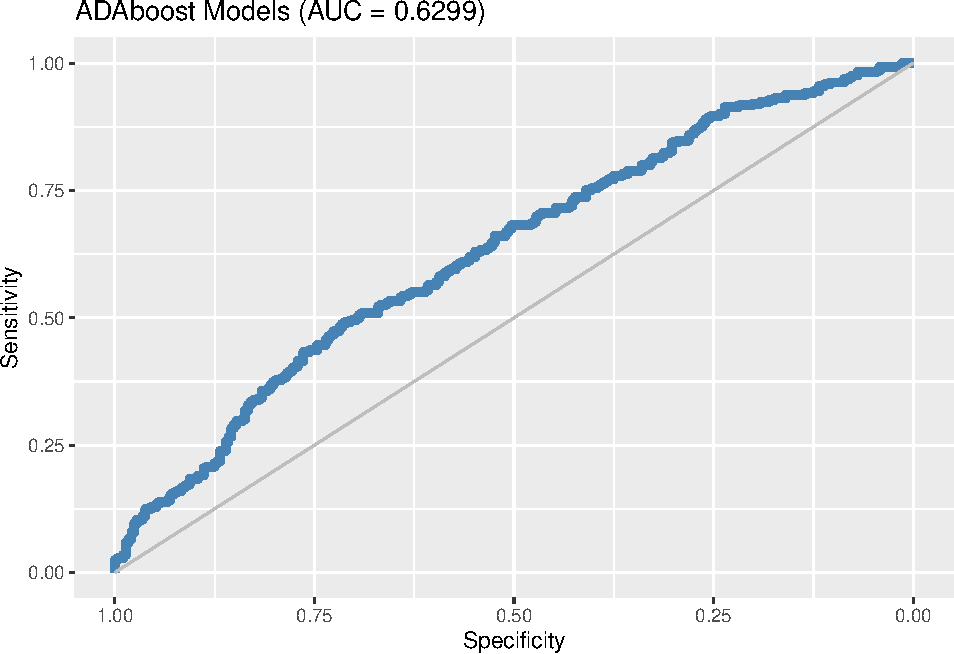
\includegraphics{07-Ensembles_of_Logistic_Models_files/figure-latex/Logistic ensemble-1.pdf}

\begin{verbatim}
#> Setting levels: control = 0, case = 1
#> Setting direction: controls < cases
#> Setting levels: control = 0, case = 1
#> Setting direction: controls < cases
\end{verbatim}

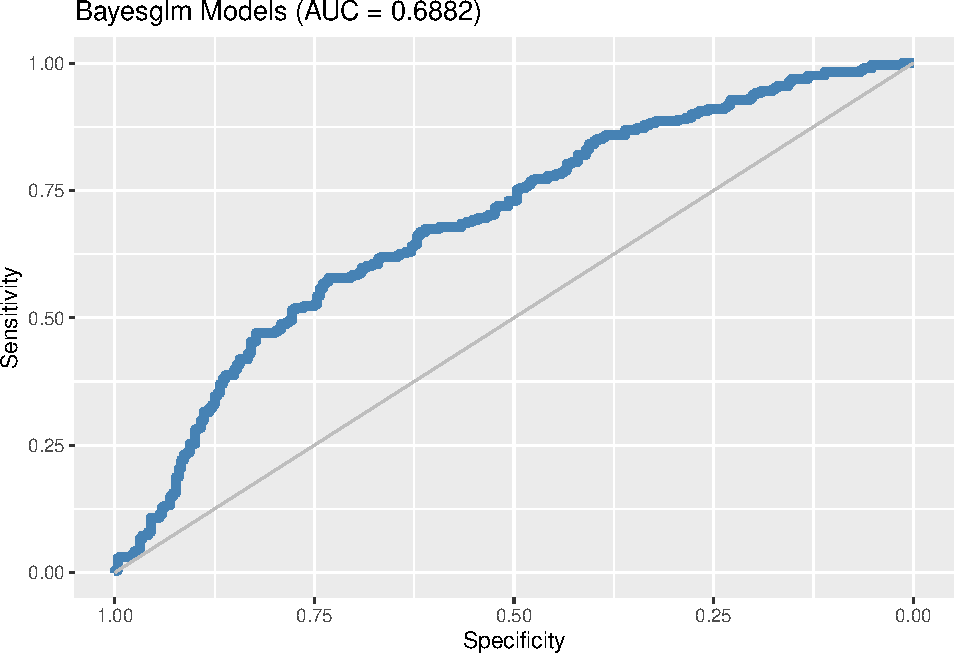
\includegraphics{07-Ensembles_of_Logistic_Models_files/figure-latex/Logistic ensemble-2.pdf}

\begin{verbatim}
#> Setting levels: control = 0, case = 1
#> Setting direction: controls < cases
#> Setting levels: control = 0, case = 1
#> Setting direction: controls < cases
\end{verbatim}

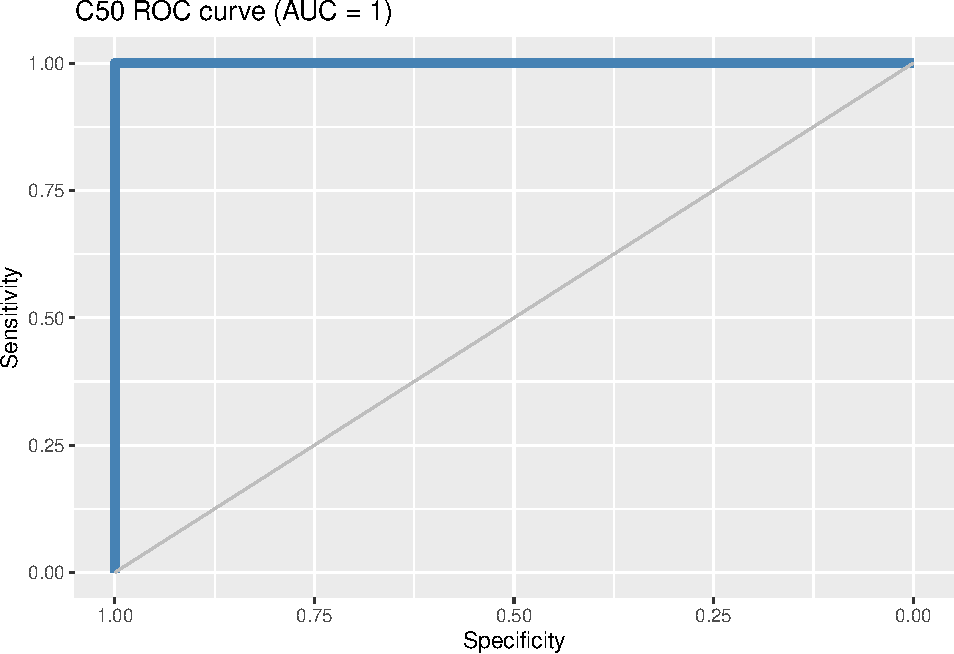
\includegraphics{07-Ensembles_of_Logistic_Models_files/figure-latex/Logistic ensemble-3.pdf}

\begin{verbatim}
#> Setting levels: control = 0, case = 1
#> Setting direction: controls < cases
#> Setting levels: control = 0, case = 1
#> Setting direction: controls < cases
\end{verbatim}

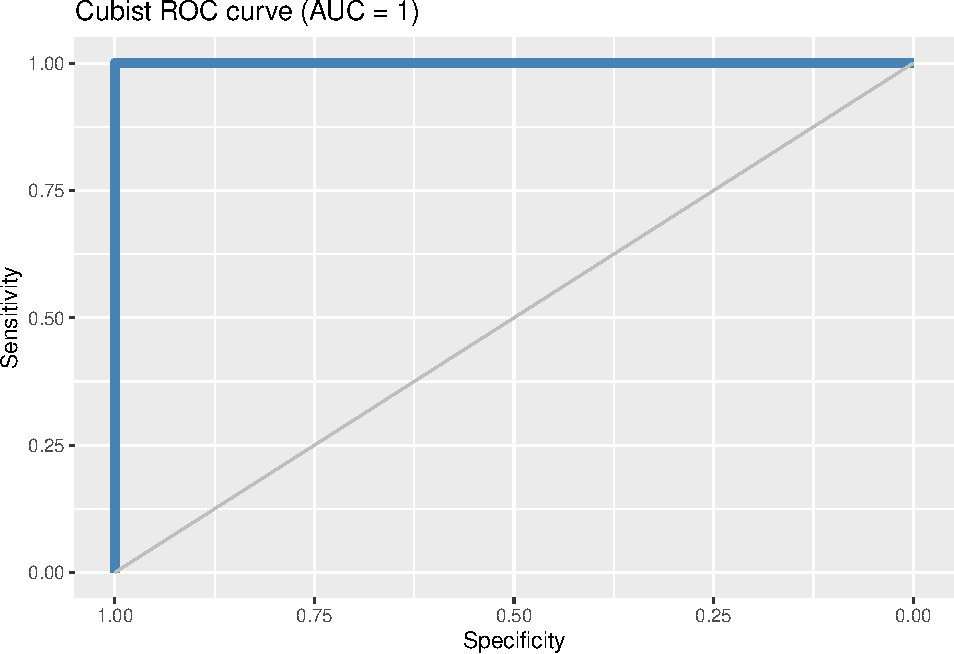
\includegraphics{07-Ensembles_of_Logistic_Models_files/figure-latex/Logistic ensemble-4.pdf}

\begin{verbatim}
#> [1]  train-rmse:0.470774 test-rmse:0.483001 
#> [2]  train-rmse:0.453550 test-rmse:0.475001 
#> [3]  train-rmse:0.442918 test-rmse:0.472652 
#> [4]  train-rmse:0.435739 test-rmse:0.472025 
#> [5]  train-rmse:0.429007 test-rmse:0.471300 
#> [6]  train-rmse:0.423949 test-rmse:0.470782 
#> [7]  train-rmse:0.420143 test-rmse:0.470954 
#> [8]  train-rmse:0.416547 test-rmse:0.472001 
#> [9]  train-rmse:0.411189 test-rmse:0.472633 
#> [10] train-rmse:0.406875 test-rmse:0.469778 
#> [11] train-rmse:0.403635 test-rmse:0.470531 
#> [12] train-rmse:0.401741 test-rmse:0.471119 
#> [13] train-rmse:0.400155 test-rmse:0.471325 
#> [14] train-rmse:0.396788 test-rmse:0.472437 
#> [15] train-rmse:0.394166 test-rmse:0.473864 
#> [16] train-rmse:0.390991 test-rmse:0.473693 
#> [17] train-rmse:0.387695 test-rmse:0.474859 
#> [18] train-rmse:0.384245 test-rmse:0.475209 
#> [19] train-rmse:0.381598 test-rmse:0.476132 
#> [20] train-rmse:0.378909 test-rmse:0.476567 
#> [21] train-rmse:0.377076 test-rmse:0.478671 
#> [22] train-rmse:0.373375 test-rmse:0.479320 
#> [23] train-rmse:0.370880 test-rmse:0.479519 
#> [24] train-rmse:0.370012 test-rmse:0.479110 
#> [25] train-rmse:0.368172 test-rmse:0.478800 
#> [26] train-rmse:0.366110 test-rmse:0.479247 
#> [27] train-rmse:0.363253 test-rmse:0.479877 
#> [28] train-rmse:0.361565 test-rmse:0.480121 
#> [29] train-rmse:0.358549 test-rmse:0.481997 
#> [30] train-rmse:0.357106 test-rmse:0.482648 
#> [31] train-rmse:0.356305 test-rmse:0.482737 
#> [32] train-rmse:0.353943 test-rmse:0.483887 
#> [33] train-rmse:0.351448 test-rmse:0.484528 
#> [34] train-rmse:0.349692 test-rmse:0.484464 
#> [35] train-rmse:0.347134 test-rmse:0.486675 
#> [36] train-rmse:0.345090 test-rmse:0.486721 
#> [37] train-rmse:0.344480 test-rmse:0.487283 
#> [38] train-rmse:0.342012 test-rmse:0.487472 
#> [39] train-rmse:0.340296 test-rmse:0.487826 
#> [40] train-rmse:0.337695 test-rmse:0.488935 
#> [41] train-rmse:0.334783 test-rmse:0.489564 
#> [42] train-rmse:0.332440 test-rmse:0.489254 
#> [43] train-rmse:0.330534 test-rmse:0.490065 
#> [44] train-rmse:0.328177 test-rmse:0.490782 
#> [45] train-rmse:0.326590 test-rmse:0.491808 
#> [46] train-rmse:0.325048 test-rmse:0.492178 
#> [47] train-rmse:0.322524 test-rmse:0.493038 
#> [48] train-rmse:0.321161 test-rmse:0.493777 
#> [49] train-rmse:0.320704 test-rmse:0.493388 
#> [50] train-rmse:0.319225 test-rmse:0.493648 
#> [51] train-rmse:0.318260 test-rmse:0.493504 
#> [52] train-rmse:0.315591 test-rmse:0.494712 
#> [53] train-rmse:0.313611 test-rmse:0.495946 
#> [54] train-rmse:0.312143 test-rmse:0.495734 
#> [55] train-rmse:0.311315 test-rmse:0.495563 
#> [56] train-rmse:0.309689 test-rmse:0.496662 
#> [57] train-rmse:0.308835 test-rmse:0.496554 
#> [58] train-rmse:0.307476 test-rmse:0.496957 
#> [59] train-rmse:0.305118 test-rmse:0.498221 
#> [60] train-rmse:0.304672 test-rmse:0.498113 
#> [61] train-rmse:0.303893 test-rmse:0.498351 
#> [62] train-rmse:0.302182 test-rmse:0.498844 
#> [63] train-rmse:0.301212 test-rmse:0.498933 
#> [64] train-rmse:0.298419 test-rmse:0.499894 
#> [65] train-rmse:0.296453 test-rmse:0.499129 
#> [66] train-rmse:0.295739 test-rmse:0.499114 
#> [67] train-rmse:0.294127 test-rmse:0.499886 
#> [68] train-rmse:0.292161 test-rmse:0.500730 
#> [69] train-rmse:0.290999 test-rmse:0.501972 
#> [70] train-rmse:0.289983 test-rmse:0.502112
#> Setting levels: control = 0, case = 1
#> Setting direction: controls < cases
#> Setting levels: control = 0, case = 1
#> Setting direction: controls < cases
\end{verbatim}

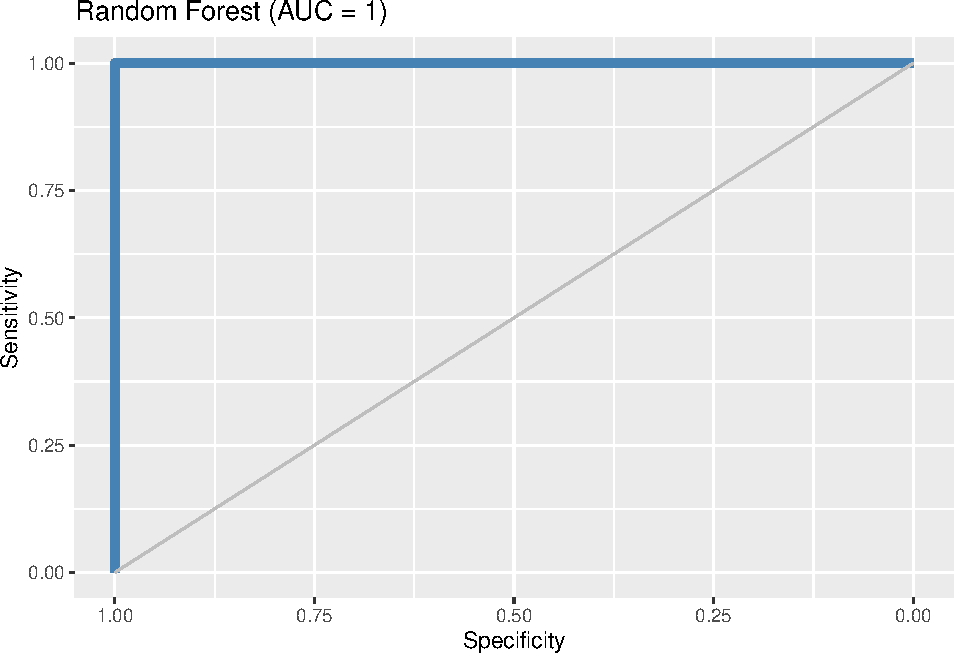
\includegraphics{07-Ensembles_of_Logistic_Models_files/figure-latex/Logistic ensemble-5.pdf}

\begin{verbatim}
#> Setting levels: control = 0, case = 1
#> Setting direction: controls < cases
#> Setting levels: control = 0, case = 1
#> Setting direction: controls < cases
\end{verbatim}

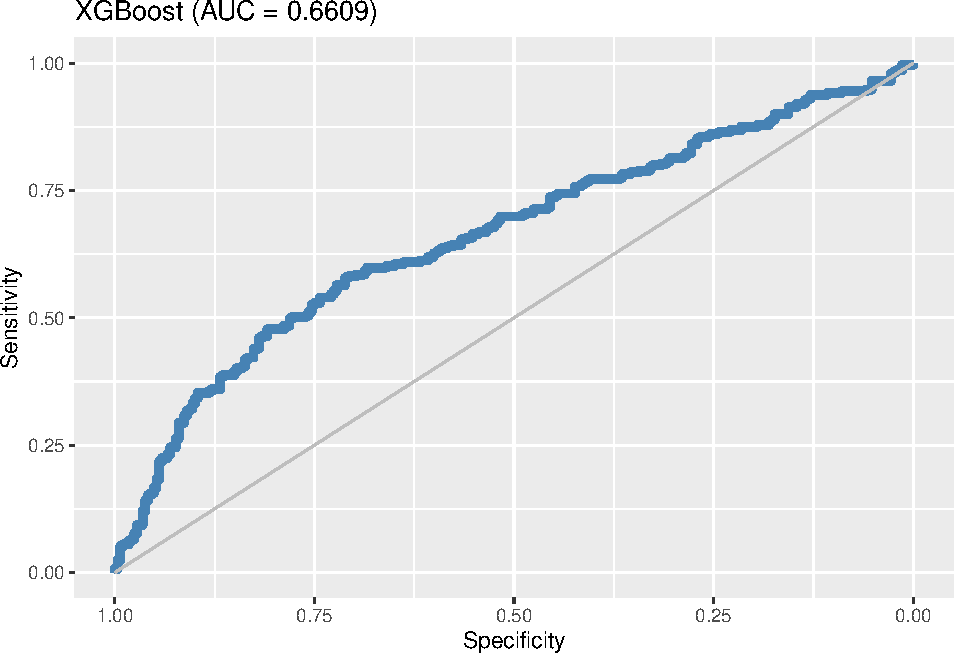
\includegraphics{07-Ensembles_of_Logistic_Models_files/figure-latex/Logistic ensemble-6.pdf}

\begin{verbatim}
#> Setting levels: control = 0, case = 1
#> Setting direction: controls < cases
#> Setting levels: control = 0, case = 1
#> Setting direction: controls < cases
\end{verbatim}

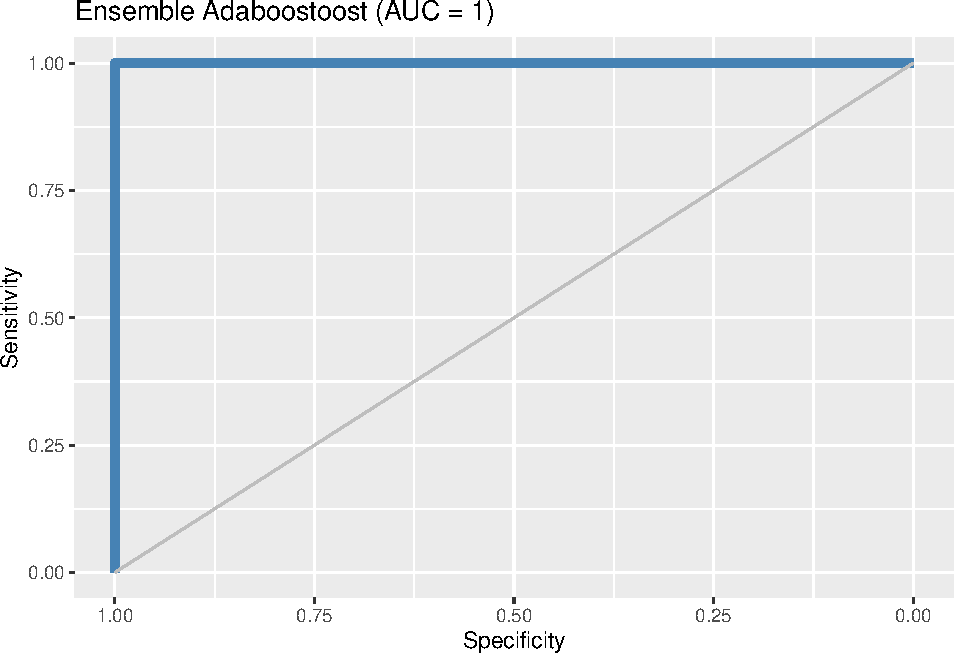
\includegraphics{07-Ensembles_of_Logistic_Models_files/figure-latex/Logistic ensemble-7.pdf}

\begin{verbatim}
#> Setting levels: control = 0, case = 1
#> Setting direction: controls < cases
#> Setting levels: control = 0, case = 1
#> Setting direction: controls < cases
\end{verbatim}

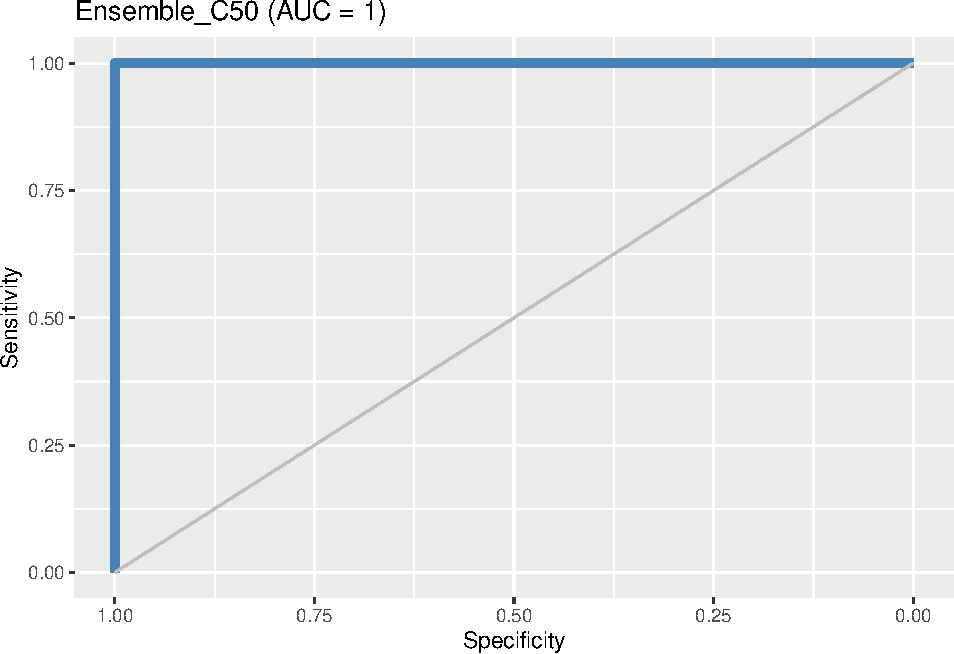
\includegraphics{07-Ensembles_of_Logistic_Models_files/figure-latex/Logistic ensemble-8.pdf}

\begin{verbatim}
#> [1]  train-rmse:0.350843 test-rmse:0.350843 
#> [2]  train-rmse:0.246181 test-rmse:0.246181 
#> [3]  train-rmse:0.172742 test-rmse:0.172742 
#> [4]  train-rmse:0.121210 test-rmse:0.121211 
#> [5]  train-rmse:0.085052 test-rmse:0.085052 
#> [6]  train-rmse:0.059679 test-rmse:0.059680 
#> [7]  train-rmse:0.041876 test-rmse:0.041876 
#> [8]  train-rmse:0.029384 test-rmse:0.029384 
#> [9]  train-rmse:0.020618 test-rmse:0.020618 
#> [10] train-rmse:0.014468 test-rmse:0.014468 
#> [11] train-rmse:0.010152 test-rmse:0.010152 
#> [12] train-rmse:0.007123 test-rmse:0.007123 
#> [13] train-rmse:0.004998 test-rmse:0.004998 
#> [14] train-rmse:0.003507 test-rmse:0.003507 
#> [15] train-rmse:0.002461 test-rmse:0.002461 
#> [16] train-rmse:0.001727 test-rmse:0.001727 
#> [17] train-rmse:0.001212 test-rmse:0.001212 
#> [18] train-rmse:0.000850 test-rmse:0.000850 
#> [19] train-rmse:0.000597 test-rmse:0.000597 
#> [20] train-rmse:0.000419 test-rmse:0.000419 
#> [21] train-rmse:0.000294 test-rmse:0.000294 
#> [22] train-rmse:0.000206 test-rmse:0.000206 
#> [23] train-rmse:0.000145 test-rmse:0.000145 
#> [24] train-rmse:0.000101 test-rmse:0.000101 
#> [25] train-rmse:0.000071 test-rmse:0.000071 
#> [26] train-rmse:0.000050 test-rmse:0.000050 
#> [27] train-rmse:0.000050 test-rmse:0.000050 
#> [28] train-rmse:0.000050 test-rmse:0.000050 
#> [29] train-rmse:0.000050 test-rmse:0.000050 
#> [30] train-rmse:0.000050 test-rmse:0.000050 
#> [31] train-rmse:0.000050 test-rmse:0.000050 
#> [32] train-rmse:0.000050 test-rmse:0.000050 
#> [33] train-rmse:0.000050 test-rmse:0.000050 
#> [34] train-rmse:0.000050 test-rmse:0.000050 
#> [35] train-rmse:0.000050 test-rmse:0.000050 
#> [36] train-rmse:0.000050 test-rmse:0.000050 
#> [37] train-rmse:0.000050 test-rmse:0.000050 
#> [38] train-rmse:0.000050 test-rmse:0.000050 
#> [39] train-rmse:0.000050 test-rmse:0.000050 
#> [40] train-rmse:0.000050 test-rmse:0.000050 
#> [41] train-rmse:0.000050 test-rmse:0.000050 
#> [42] train-rmse:0.000050 test-rmse:0.000050 
#> [43] train-rmse:0.000050 test-rmse:0.000050 
#> [44] train-rmse:0.000050 test-rmse:0.000050 
#> [45] train-rmse:0.000050 test-rmse:0.000050 
#> [46] train-rmse:0.000050 test-rmse:0.000050 
#> [47] train-rmse:0.000050 test-rmse:0.000050 
#> [48] train-rmse:0.000050 test-rmse:0.000050 
#> [49] train-rmse:0.000050 test-rmse:0.000050 
#> [50] train-rmse:0.000050 test-rmse:0.000050 
#> [51] train-rmse:0.000050 test-rmse:0.000050 
#> [52] train-rmse:0.000050 test-rmse:0.000050 
#> [53] train-rmse:0.000050 test-rmse:0.000050 
#> [54] train-rmse:0.000050 test-rmse:0.000050 
#> [55] train-rmse:0.000050 test-rmse:0.000050 
#> [56] train-rmse:0.000050 test-rmse:0.000050 
#> [57] train-rmse:0.000050 test-rmse:0.000050 
#> [58] train-rmse:0.000050 test-rmse:0.000050 
#> [59] train-rmse:0.000050 test-rmse:0.000050 
#> [60] train-rmse:0.000050 test-rmse:0.000050 
#> [61] train-rmse:0.000050 test-rmse:0.000050 
#> [62] train-rmse:0.000050 test-rmse:0.000050 
#> [63] train-rmse:0.000050 test-rmse:0.000050 
#> [64] train-rmse:0.000050 test-rmse:0.000050 
#> [65] train-rmse:0.000050 test-rmse:0.000050 
#> [66] train-rmse:0.000050 test-rmse:0.000050 
#> [67] train-rmse:0.000050 test-rmse:0.000050 
#> [68] train-rmse:0.000050 test-rmse:0.000050 
#> [69] train-rmse:0.000050 test-rmse:0.000050 
#> [70] train-rmse:0.000050 test-rmse:0.000050
#> Setting levels: control = 0, case = 1
#> Setting direction: controls < cases
#> Setting levels: control = 0, case = 1
#> Setting direction: controls < cases
\end{verbatim}

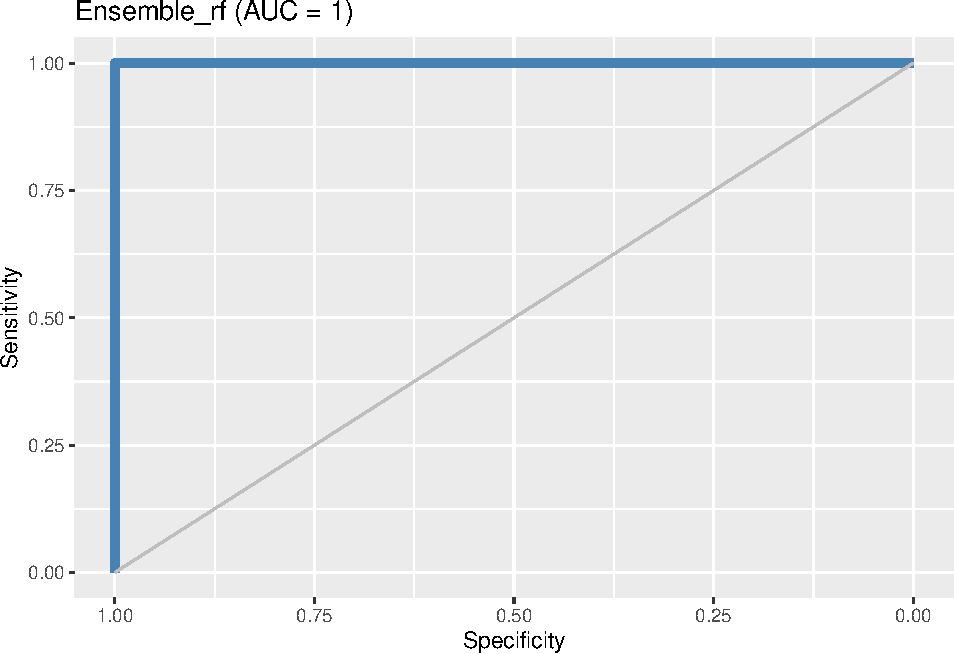
\includegraphics{07-Ensembles_of_Logistic_Models_files/figure-latex/Logistic ensemble-9.pdf}

\begin{verbatim}
#> Setting levels: control = 0, case = 1
#> Setting direction: controls < cases
#> Setting levels: control = 0, case = 1
#> Setting direction: controls < cases
\end{verbatim}

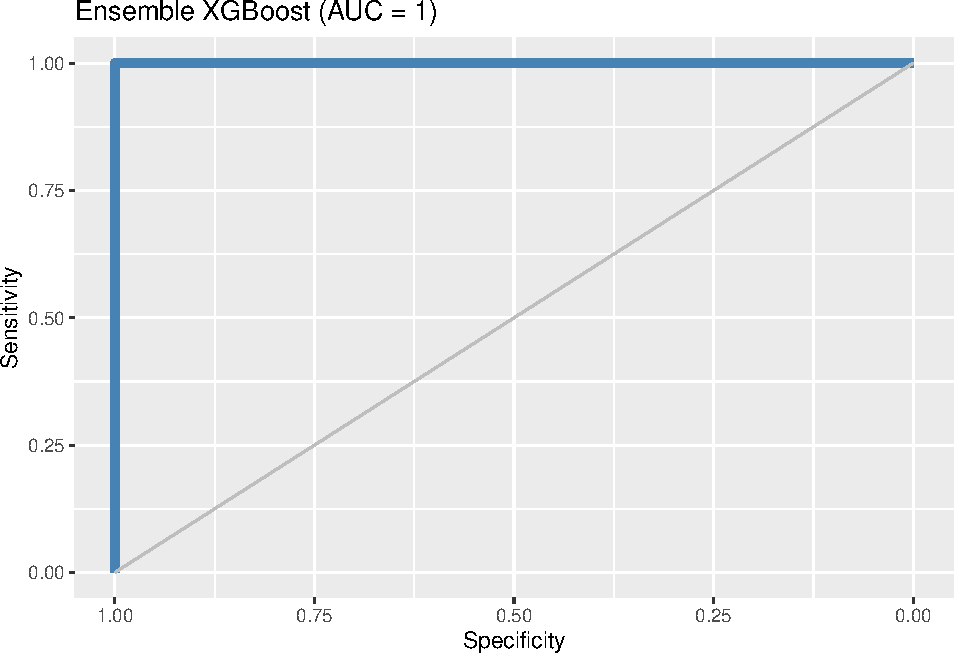
\includegraphics{07-Ensembles_of_Logistic_Models_files/figure-latex/Logistic ensemble-10.pdf}

\begin{verbatim}
#> Setting levels: control = 0, case = 1
#> Setting direction: controls < cases
#> Setting levels: control = 0, case = 1
#> Setting direction: controls < cases
\end{verbatim}

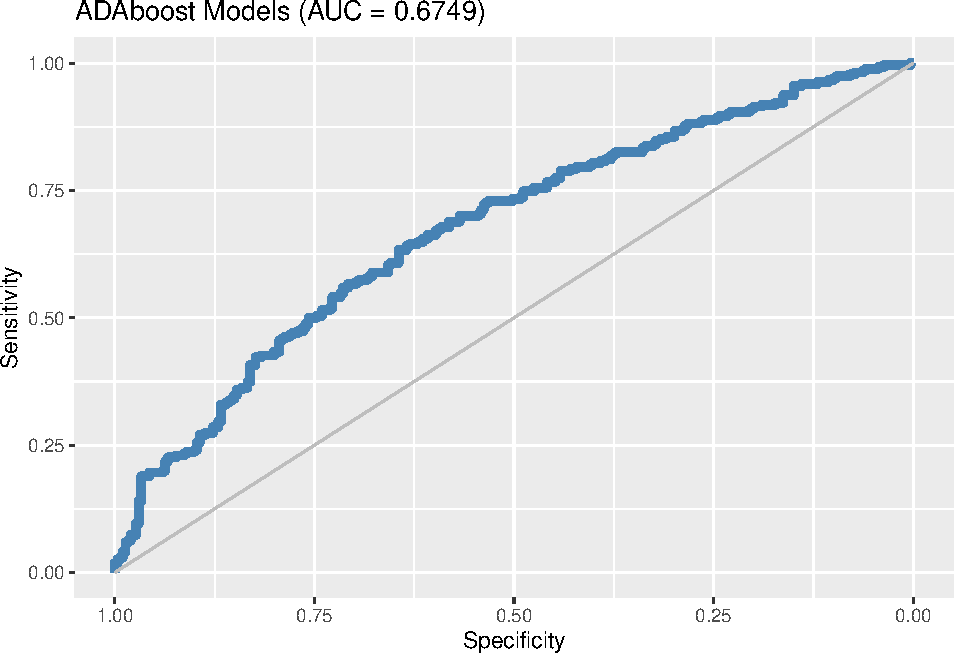
\includegraphics{07-Ensembles_of_Logistic_Models_files/figure-latex/Logistic ensemble-11.pdf}

\begin{verbatim}
#> Setting levels: control = 0, case = 1
#> Setting direction: controls < cases
#> Setting levels: control = 0, case = 1
#> Setting direction: controls < cases
\end{verbatim}

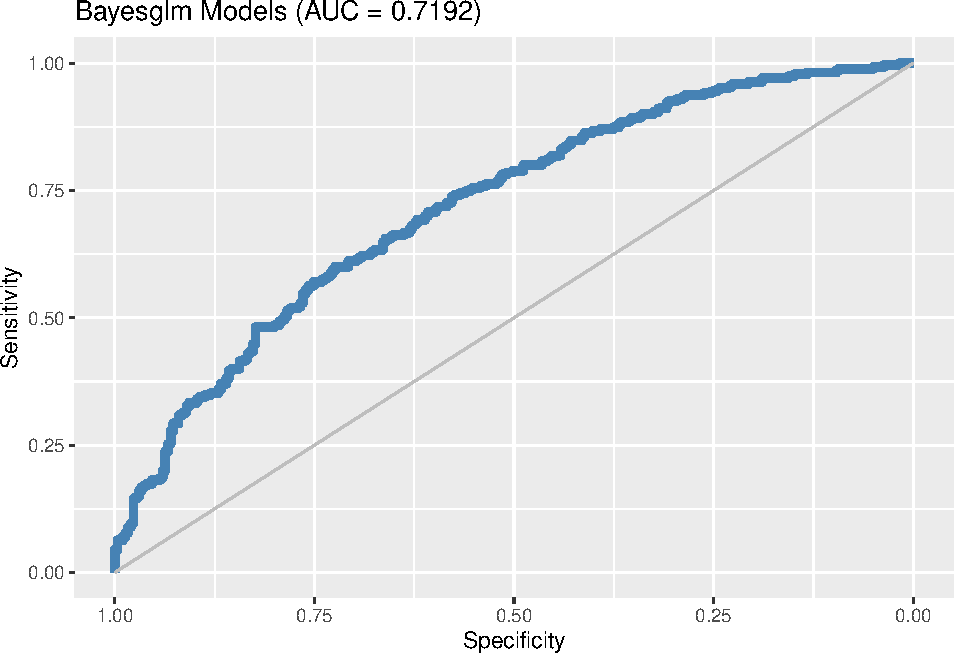
\includegraphics{07-Ensembles_of_Logistic_Models_files/figure-latex/Logistic ensemble-12.pdf}

\begin{verbatim}
#> Setting levels: control = 0, case = 1
#> Setting direction: controls < cases
#> Setting levels: control = 0, case = 1
#> Setting direction: controls < cases
\end{verbatim}

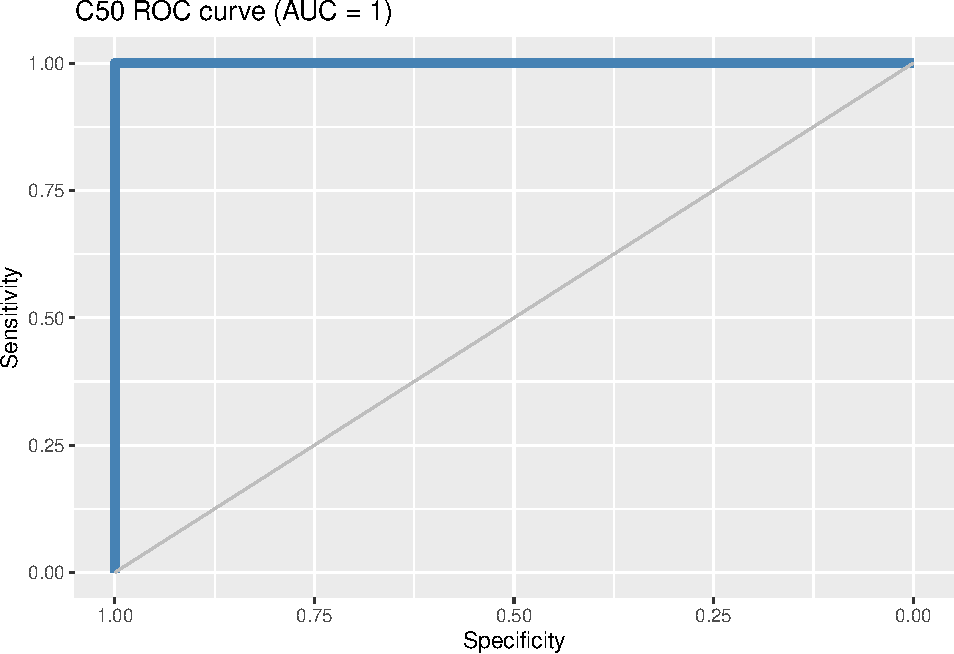
\includegraphics{07-Ensembles_of_Logistic_Models_files/figure-latex/Logistic ensemble-13.pdf}

\begin{verbatim}
#> Setting levels: control = 0, case = 1
#> Setting direction: controls < cases
#> Setting levels: control = 0, case = 1
#> Setting direction: controls < cases
\end{verbatim}

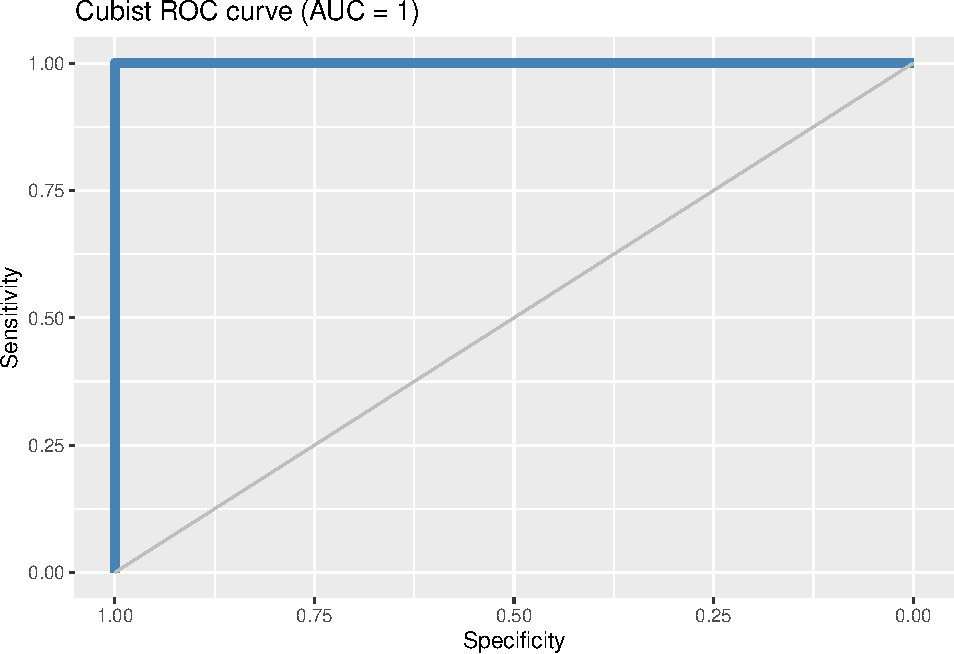
\includegraphics{07-Ensembles_of_Logistic_Models_files/figure-latex/Logistic ensemble-14.pdf}

\begin{verbatim}
#> [1]  train-rmse:0.475494 test-rmse:0.478977 
#> [2]  train-rmse:0.461308 test-rmse:0.467409 
#> [3]  train-rmse:0.451290 test-rmse:0.460698 
#> [4]  train-rmse:0.444832 test-rmse:0.458742 
#> [5]  train-rmse:0.440894 test-rmse:0.454982 
#> [6]  train-rmse:0.436131 test-rmse:0.455092 
#> [7]  train-rmse:0.432023 test-rmse:0.456360 
#> [8]  train-rmse:0.430608 test-rmse:0.455371 
#> [9]  train-rmse:0.427672 test-rmse:0.454953 
#> [10] train-rmse:0.425378 test-rmse:0.454318 
#> [11] train-rmse:0.421327 test-rmse:0.454782 
#> [12] train-rmse:0.419311 test-rmse:0.455231 
#> [13] train-rmse:0.415492 test-rmse:0.456923 
#> [14] train-rmse:0.414885 test-rmse:0.456328 
#> [15] train-rmse:0.412060 test-rmse:0.457881 
#> [16] train-rmse:0.410805 test-rmse:0.458040 
#> [17] train-rmse:0.409671 test-rmse:0.458004 
#> [18] train-rmse:0.406705 test-rmse:0.456977 
#> [19] train-rmse:0.403390 test-rmse:0.457402 
#> [20] train-rmse:0.399627 test-rmse:0.456932 
#> [21] train-rmse:0.397204 test-rmse:0.457170 
#> [22] train-rmse:0.395173 test-rmse:0.456266 
#> [23] train-rmse:0.393567 test-rmse:0.455977 
#> [24] train-rmse:0.391434 test-rmse:0.456980 
#> [25] train-rmse:0.391096 test-rmse:0.456632 
#> [26] train-rmse:0.388087 test-rmse:0.457460 
#> [27] train-rmse:0.386282 test-rmse:0.457303 
#> [28] train-rmse:0.384305 test-rmse:0.457527 
#> [29] train-rmse:0.382029 test-rmse:0.457662 
#> [30] train-rmse:0.379441 test-rmse:0.457910 
#> [31] train-rmse:0.378254 test-rmse:0.458667 
#> [32] train-rmse:0.375774 test-rmse:0.458768 
#> [33] train-rmse:0.373497 test-rmse:0.458288 
#> [34] train-rmse:0.371587 test-rmse:0.458543 
#> [35] train-rmse:0.369425 test-rmse:0.458635 
#> [36] train-rmse:0.366356 test-rmse:0.458635 
#> [37] train-rmse:0.365787 test-rmse:0.459434 
#> [38] train-rmse:0.364950 test-rmse:0.458543 
#> [39] train-rmse:0.362337 test-rmse:0.459058 
#> [40] train-rmse:0.360853 test-rmse:0.460159 
#> [41] train-rmse:0.357652 test-rmse:0.461202 
#> [42] train-rmse:0.356950 test-rmse:0.460875 
#> [43] train-rmse:0.355019 test-rmse:0.460435 
#> [44] train-rmse:0.353211 test-rmse:0.460436 
#> [45] train-rmse:0.351071 test-rmse:0.461266 
#> [46] train-rmse:0.349073 test-rmse:0.461159 
#> [47] train-rmse:0.347402 test-rmse:0.461330 
#> [48] train-rmse:0.344948 test-rmse:0.462809 
#> [49] train-rmse:0.342786 test-rmse:0.462840 
#> [50] train-rmse:0.340665 test-rmse:0.464042 
#> [51] train-rmse:0.339733 test-rmse:0.463679 
#> [52] train-rmse:0.339251 test-rmse:0.463389 
#> [53] train-rmse:0.337479 test-rmse:0.463276 
#> [54] train-rmse:0.334147 test-rmse:0.463642 
#> [55] train-rmse:0.332583 test-rmse:0.465007 
#> [56] train-rmse:0.331482 test-rmse:0.465319 
#> [57] train-rmse:0.330276 test-rmse:0.465422 
#> [58] train-rmse:0.328943 test-rmse:0.464523 
#> [59] train-rmse:0.327458 test-rmse:0.464478 
#> [60] train-rmse:0.326050 test-rmse:0.464181 
#> [61] train-rmse:0.325237 test-rmse:0.463910 
#> [62] train-rmse:0.323923 test-rmse:0.464489 
#> [63] train-rmse:0.321625 test-rmse:0.464686 
#> [64] train-rmse:0.320839 test-rmse:0.464667 
#> [65] train-rmse:0.319611 test-rmse:0.465104 
#> [66] train-rmse:0.318031 test-rmse:0.465275 
#> [67] train-rmse:0.317079 test-rmse:0.465033 
#> [68] train-rmse:0.316594 test-rmse:0.464572 
#> [69] train-rmse:0.316099 test-rmse:0.464694 
#> [70] train-rmse:0.315826 test-rmse:0.464827
#> Setting levels: control = 0, case = 1
#> Setting direction: controls < cases
#> Setting levels: control = 0, case = 1
#> Setting direction: controls < cases
\end{verbatim}

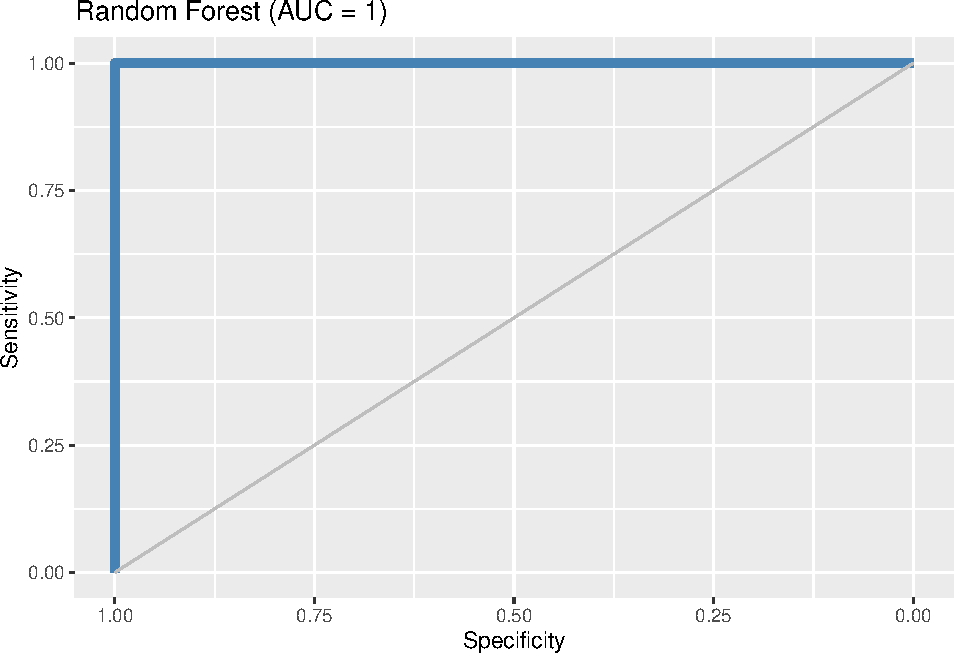
\includegraphics{07-Ensembles_of_Logistic_Models_files/figure-latex/Logistic ensemble-15.pdf}

\begin{verbatim}
#> Setting levels: control = 0, case = 1
#> Setting direction: controls < cases
#> Setting levels: control = 0, case = 1
#> Setting direction: controls < cases
\end{verbatim}

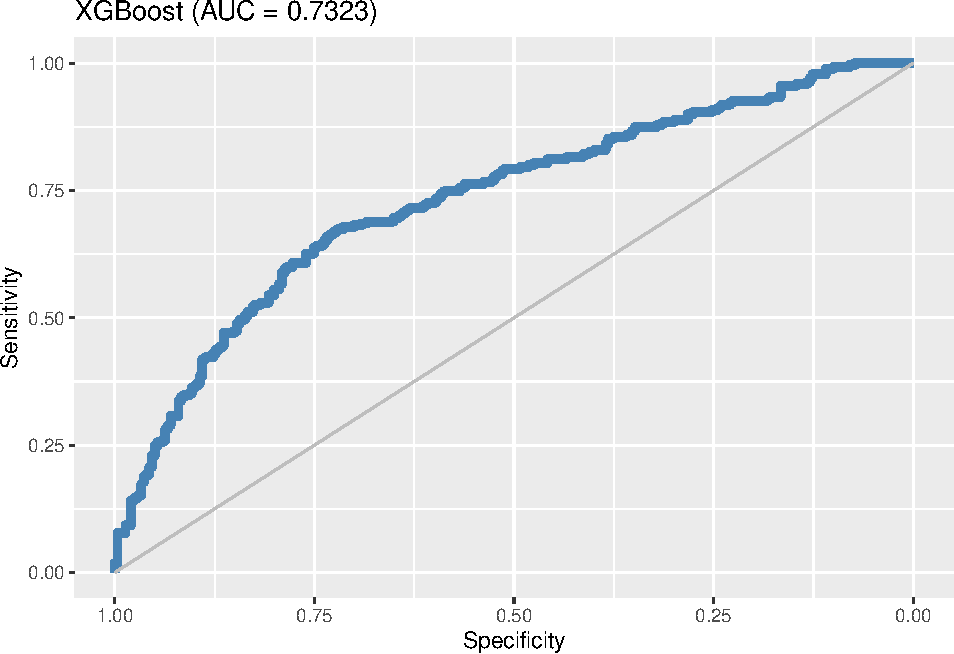
\includegraphics{07-Ensembles_of_Logistic_Models_files/figure-latex/Logistic ensemble-16.pdf}

\begin{verbatim}
#> Setting levels: control = 0, case = 1
#> Setting direction: controls < cases
#> Setting levels: control = 0, case = 1
#> Setting direction: controls < cases
\end{verbatim}

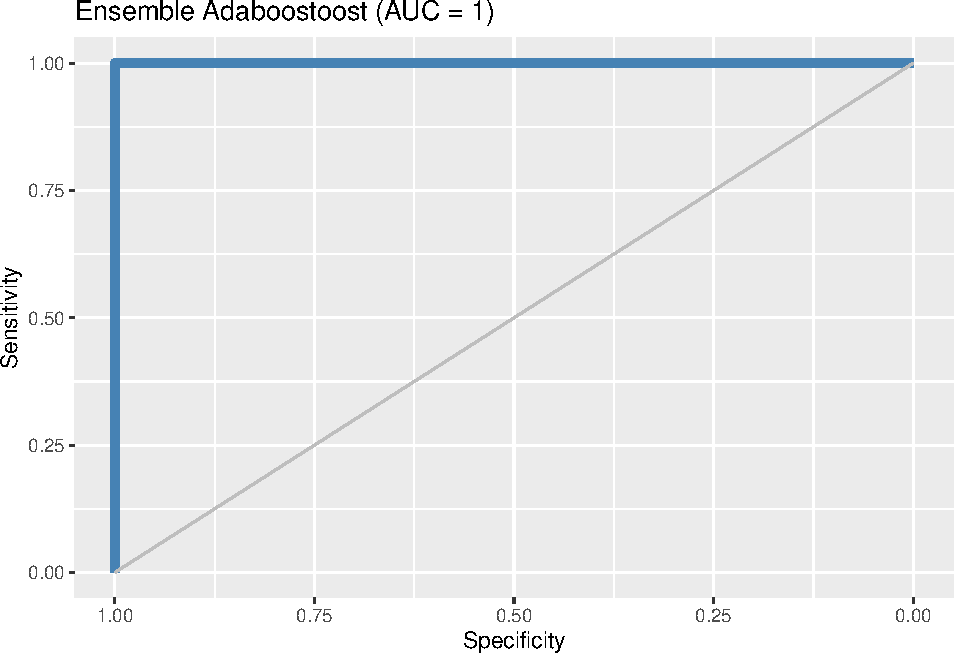
\includegraphics{07-Ensembles_of_Logistic_Models_files/figure-latex/Logistic ensemble-17.pdf}

\begin{verbatim}
#> Setting levels: control = 0, case = 1
#> Setting direction: controls < cases
#> Setting levels: control = 0, case = 1
#> Setting direction: controls < cases
\end{verbatim}

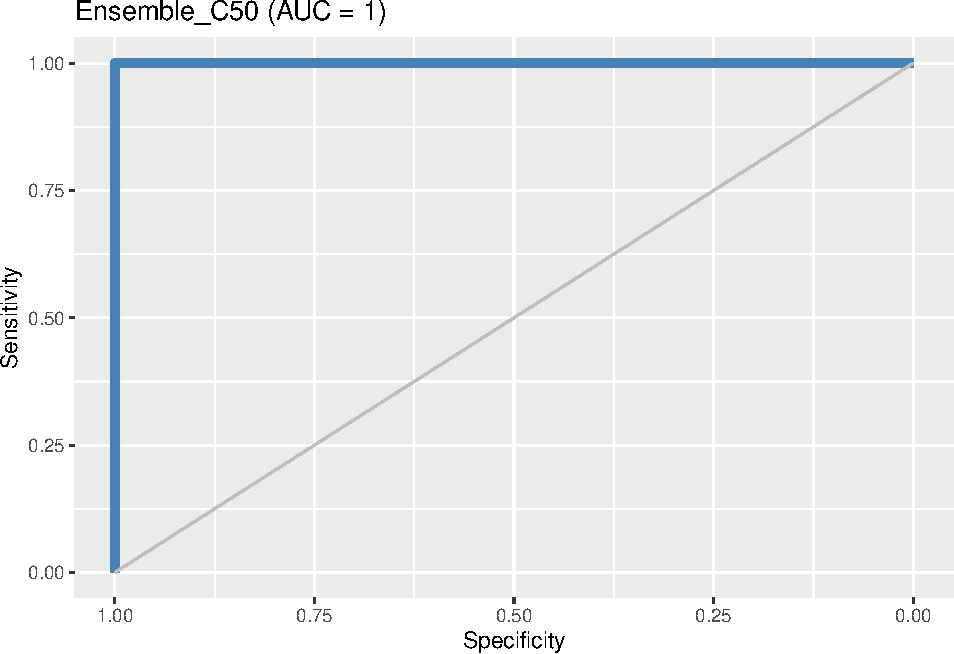
\includegraphics{07-Ensembles_of_Logistic_Models_files/figure-latex/Logistic ensemble-18.pdf}

\begin{verbatim}
#> [1]  train-rmse:0.350888 test-rmse:0.350893 
#> [2]  train-rmse:0.246244 test-rmse:0.246251 
#> [3]  train-rmse:0.172808 test-rmse:0.172816 
#> [4]  train-rmse:0.121272 test-rmse:0.121280 
#> [5]  train-rmse:0.085106 test-rmse:0.085112 
#> [6]  train-rmse:0.059725 test-rmse:0.059731 
#> [7]  train-rmse:0.041914 test-rmse:0.041918 
#> [8]  train-rmse:0.029414 test-rmse:0.029418 
#> [9]  train-rmse:0.020642 test-rmse:0.020645 
#> [10] train-rmse:0.014486 test-rmse:0.014488 
#> [11] train-rmse:0.010166 test-rmse:0.010168 
#> [12] train-rmse:0.007134 test-rmse:0.007135 
#> [13] train-rmse:0.005007 test-rmse:0.005008 
#> [14] train-rmse:0.003514 test-rmse:0.003514 
#> [15] train-rmse:0.002466 test-rmse:0.002466 
#> [16] train-rmse:0.001730 test-rmse:0.001731 
#> [17] train-rmse:0.001214 test-rmse:0.001215 
#> [18] train-rmse:0.000852 test-rmse:0.000852 
#> [19] train-rmse:0.000598 test-rmse:0.000598 
#> [20] train-rmse:0.000420 test-rmse:0.000420 
#> [21] train-rmse:0.000295 test-rmse:0.000295 
#> [22] train-rmse:0.000207 test-rmse:0.000207 
#> [23] train-rmse:0.000145 test-rmse:0.000145 
#> [24] train-rmse:0.000102 test-rmse:0.000102 
#> [25] train-rmse:0.000071 test-rmse:0.000071 
#> [26] train-rmse:0.000050 test-rmse:0.000050 
#> [27] train-rmse:0.000050 test-rmse:0.000050 
#> [28] train-rmse:0.000050 test-rmse:0.000050 
#> [29] train-rmse:0.000050 test-rmse:0.000050 
#> [30] train-rmse:0.000050 test-rmse:0.000050 
#> [31] train-rmse:0.000050 test-rmse:0.000050 
#> [32] train-rmse:0.000050 test-rmse:0.000050 
#> [33] train-rmse:0.000050 test-rmse:0.000050 
#> [34] train-rmse:0.000050 test-rmse:0.000050 
#> [35] train-rmse:0.000050 test-rmse:0.000050 
#> [36] train-rmse:0.000050 test-rmse:0.000050 
#> [37] train-rmse:0.000050 test-rmse:0.000050 
#> [38] train-rmse:0.000050 test-rmse:0.000050 
#> [39] train-rmse:0.000050 test-rmse:0.000050 
#> [40] train-rmse:0.000050 test-rmse:0.000050 
#> [41] train-rmse:0.000050 test-rmse:0.000050 
#> [42] train-rmse:0.000050 test-rmse:0.000050 
#> [43] train-rmse:0.000050 test-rmse:0.000050 
#> [44] train-rmse:0.000050 test-rmse:0.000050 
#> [45] train-rmse:0.000050 test-rmse:0.000050 
#> [46] train-rmse:0.000050 test-rmse:0.000050 
#> [47] train-rmse:0.000050 test-rmse:0.000050 
#> [48] train-rmse:0.000050 test-rmse:0.000050 
#> [49] train-rmse:0.000050 test-rmse:0.000050 
#> [50] train-rmse:0.000050 test-rmse:0.000050 
#> [51] train-rmse:0.000050 test-rmse:0.000050 
#> [52] train-rmse:0.000050 test-rmse:0.000050 
#> [53] train-rmse:0.000050 test-rmse:0.000050 
#> [54] train-rmse:0.000050 test-rmse:0.000050 
#> [55] train-rmse:0.000050 test-rmse:0.000050 
#> [56] train-rmse:0.000050 test-rmse:0.000050 
#> [57] train-rmse:0.000050 test-rmse:0.000050 
#> [58] train-rmse:0.000050 test-rmse:0.000050 
#> [59] train-rmse:0.000050 test-rmse:0.000050 
#> [60] train-rmse:0.000050 test-rmse:0.000050 
#> [61] train-rmse:0.000050 test-rmse:0.000050 
#> [62] train-rmse:0.000050 test-rmse:0.000050 
#> [63] train-rmse:0.000050 test-rmse:0.000050 
#> [64] train-rmse:0.000050 test-rmse:0.000050 
#> [65] train-rmse:0.000050 test-rmse:0.000050 
#> [66] train-rmse:0.000050 test-rmse:0.000050 
#> [67] train-rmse:0.000050 test-rmse:0.000050 
#> [68] train-rmse:0.000050 test-rmse:0.000050 
#> [69] train-rmse:0.000050 test-rmse:0.000050 
#> [70] train-rmse:0.000050 test-rmse:0.000050
#> Setting levels: control = 0, case = 1
#> Setting direction: controls < cases
#> Setting levels: control = 0, case = 1
#> Setting direction: controls < cases
\end{verbatim}

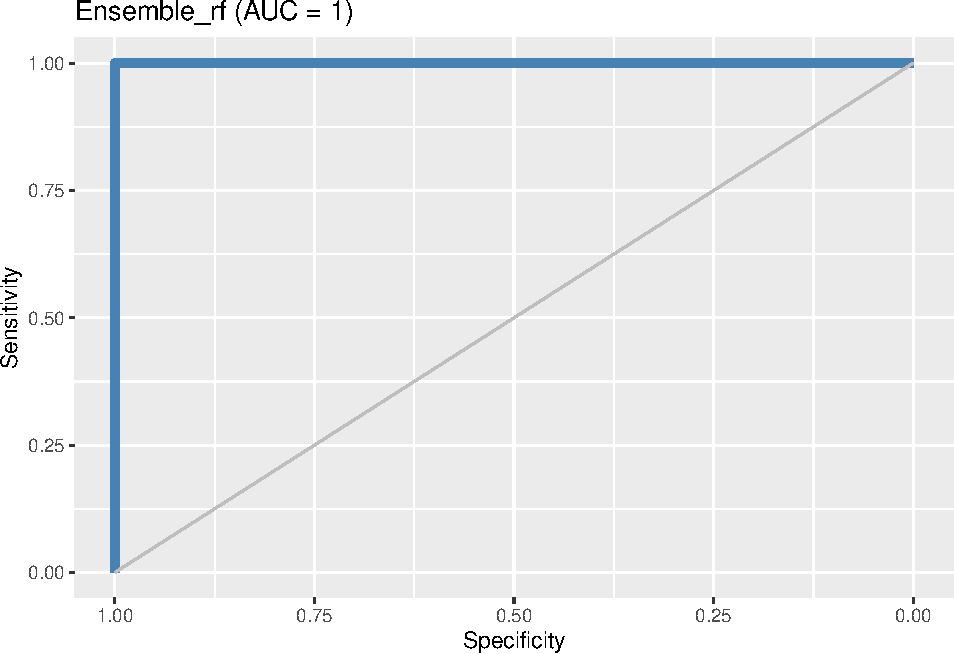
\includegraphics{07-Ensembles_of_Logistic_Models_files/figure-latex/Logistic ensemble-19.pdf}

\begin{verbatim}
#> Setting levels: control = 0, case = 1
#> Setting direction: controls < cases
#> Setting levels: control = 0, case = 1
#> Setting direction: controls < cases
\end{verbatim}

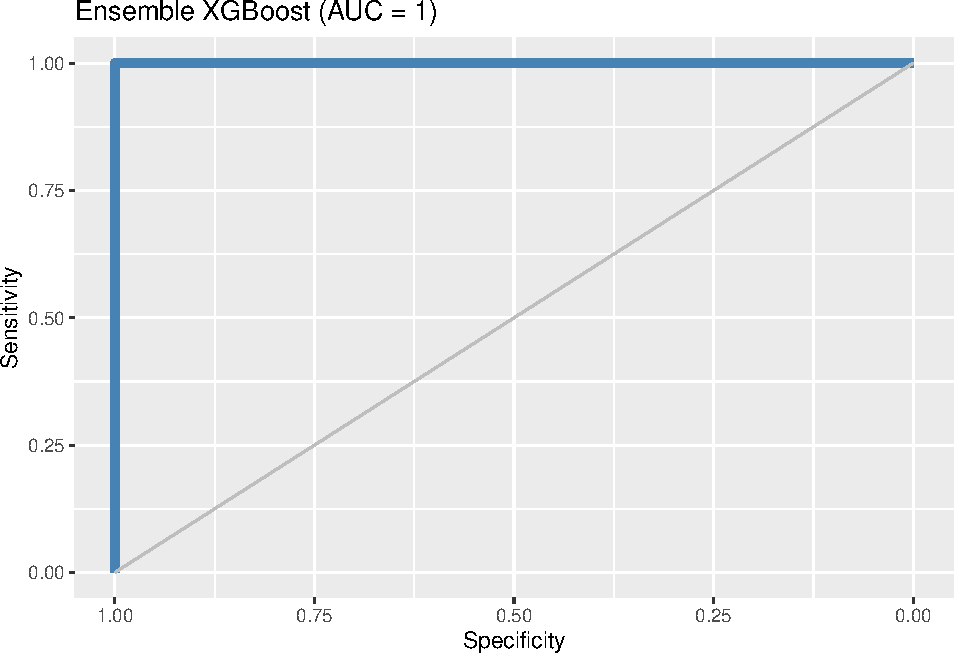
\includegraphics{07-Ensembles_of_Logistic_Models_files/figure-latex/Logistic ensemble-20.pdf}

\begin{verbatim}
#> Setting levels: control = 0, case = 1
#> Setting direction: controls < cases
#> Setting levels: control = 0, case = 1
#> Setting direction: controls < cases
\end{verbatim}

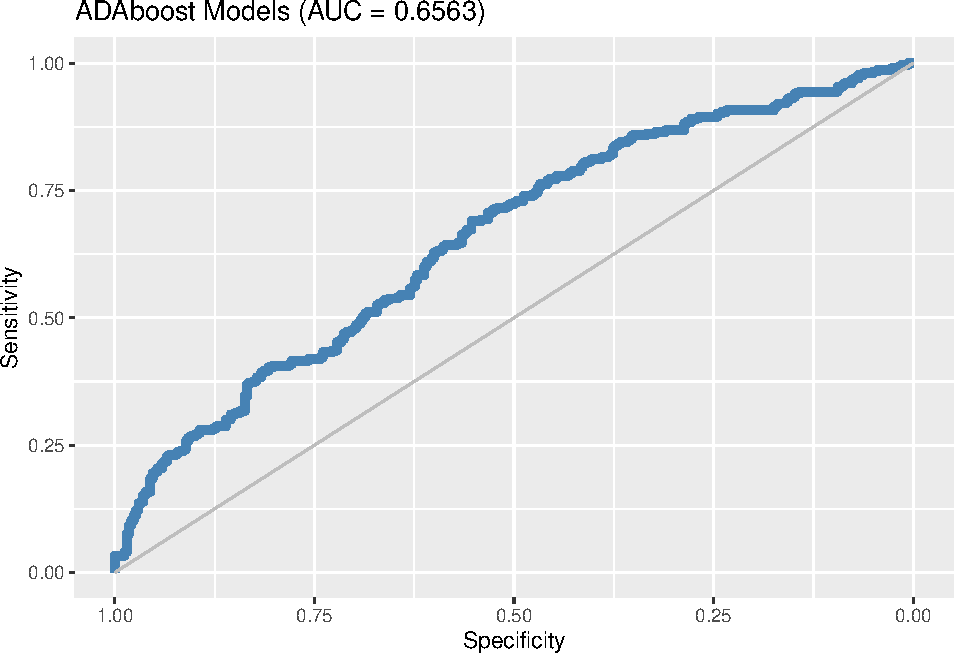
\includegraphics{07-Ensembles_of_Logistic_Models_files/figure-latex/Logistic ensemble-21.pdf}

\begin{verbatim}
#> Setting levels: control = 0, case = 1
#> Setting direction: controls < cases
#> Setting levels: control = 0, case = 1
#> Setting direction: controls < cases
\end{verbatim}

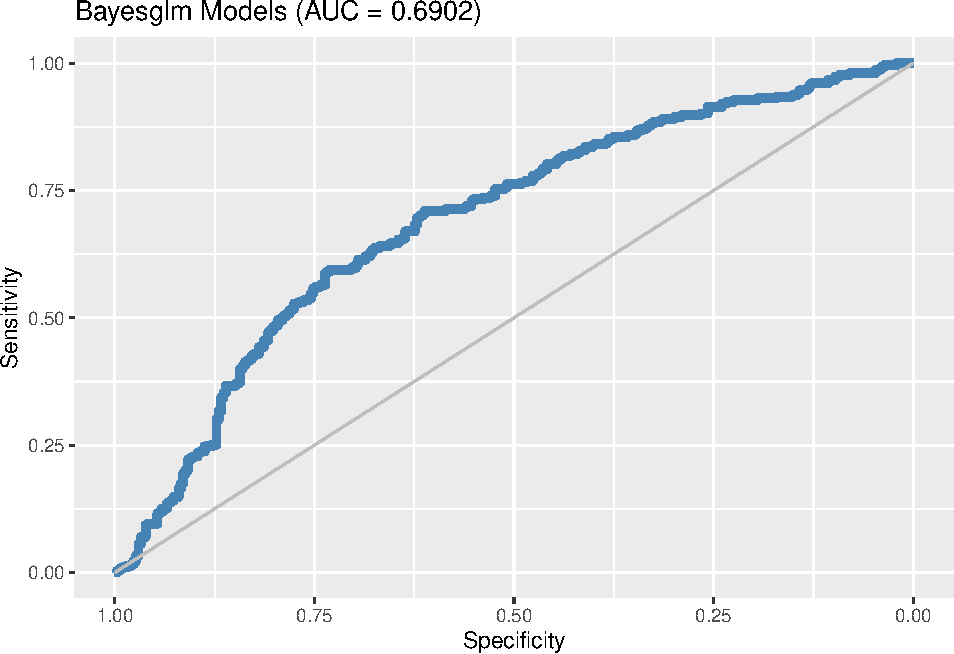
\includegraphics{07-Ensembles_of_Logistic_Models_files/figure-latex/Logistic ensemble-22.pdf}

\begin{verbatim}
#> Setting levels: control = 0, case = 1
#> Setting direction: controls < cases
#> Setting levels: control = 0, case = 1
#> Setting direction: controls < cases
\end{verbatim}

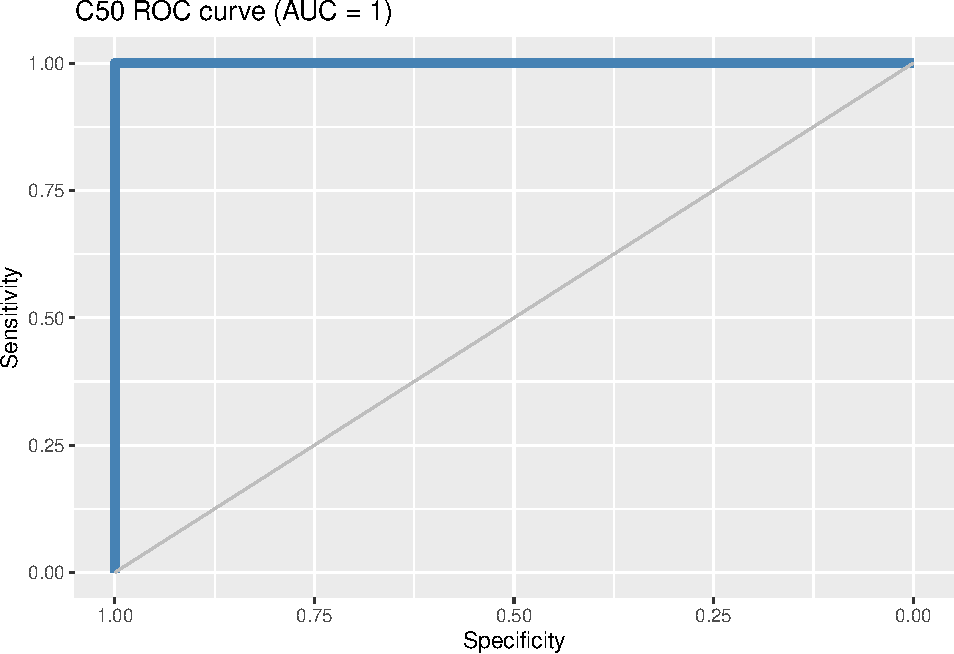
\includegraphics{07-Ensembles_of_Logistic_Models_files/figure-latex/Logistic ensemble-23.pdf}

\begin{verbatim}
#> Setting levels: control = 0, case = 1
#> Setting direction: controls < cases
#> Setting levels: control = 0, case = 1
#> Setting direction: controls < cases
\end{verbatim}

\includegraphics{07-Ensembles_of_Logistic_Models_files/figure-latex/Logistic ensemble-24.pdf}

\begin{verbatim}
#> [1]  train-rmse:0.472429 test-rmse:0.482093 
#> [2]  train-rmse:0.455873 test-rmse:0.472666 
#> [3]  train-rmse:0.445721 test-rmse:0.468027 
#> [4]  train-rmse:0.437799 test-rmse:0.465129 
#> [5]  train-rmse:0.432486 test-rmse:0.464207 
#> [6]  train-rmse:0.427021 test-rmse:0.463652 
#> [7]  train-rmse:0.422370 test-rmse:0.464937 
#> [8]  train-rmse:0.420243 test-rmse:0.464003 
#> [9]  train-rmse:0.416318 test-rmse:0.462371 
#> [10] train-rmse:0.412624 test-rmse:0.461761 
#> [11] train-rmse:0.409565 test-rmse:0.463028 
#> [12] train-rmse:0.405705 test-rmse:0.463100 
#> [13] train-rmse:0.402939 test-rmse:0.461776 
#> [14] train-rmse:0.398826 test-rmse:0.463719 
#> [15] train-rmse:0.394727 test-rmse:0.464543 
#> [16] train-rmse:0.391869 test-rmse:0.464668 
#> [17] train-rmse:0.388255 test-rmse:0.465758 
#> [18] train-rmse:0.384911 test-rmse:0.466256 
#> [19] train-rmse:0.382203 test-rmse:0.467340 
#> [20] train-rmse:0.379677 test-rmse:0.468777 
#> [21] train-rmse:0.376428 test-rmse:0.467681 
#> [22] train-rmse:0.374653 test-rmse:0.467923 
#> [23] train-rmse:0.371156 test-rmse:0.468824 
#> [24] train-rmse:0.369905 test-rmse:0.469107 
#> [25] train-rmse:0.367721 test-rmse:0.468583 
#> [26] train-rmse:0.365831 test-rmse:0.468754 
#> [27] train-rmse:0.363615 test-rmse:0.470188 
#> [28] train-rmse:0.361615 test-rmse:0.470667 
#> [29] train-rmse:0.359996 test-rmse:0.471305 
#> [30] train-rmse:0.357348 test-rmse:0.471708 
#> [31] train-rmse:0.356760 test-rmse:0.471618 
#> [32] train-rmse:0.354260 test-rmse:0.472853 
#> [33] train-rmse:0.351851 test-rmse:0.472219 
#> [34] train-rmse:0.349188 test-rmse:0.473726 
#> [35] train-rmse:0.347215 test-rmse:0.473590 
#> [36] train-rmse:0.345621 test-rmse:0.473767 
#> [37] train-rmse:0.343102 test-rmse:0.474566 
#> [38] train-rmse:0.341812 test-rmse:0.475195 
#> [39] train-rmse:0.340438 test-rmse:0.475004 
#> [40] train-rmse:0.338714 test-rmse:0.475294 
#> [41] train-rmse:0.336497 test-rmse:0.475755 
#> [42] train-rmse:0.334445 test-rmse:0.475396 
#> [43] train-rmse:0.332653 test-rmse:0.475703 
#> [44] train-rmse:0.331589 test-rmse:0.475749 
#> [45] train-rmse:0.329594 test-rmse:0.475538 
#> [46] train-rmse:0.327838 test-rmse:0.474951 
#> [47] train-rmse:0.326378 test-rmse:0.475410 
#> [48] train-rmse:0.324227 test-rmse:0.476530 
#> [49] train-rmse:0.321979 test-rmse:0.478064 
#> [50] train-rmse:0.320865 test-rmse:0.479034 
#> [51] train-rmse:0.318448 test-rmse:0.478713 
#> [52] train-rmse:0.317117 test-rmse:0.479115 
#> [53] train-rmse:0.315340 test-rmse:0.479111 
#> [54] train-rmse:0.313437 test-rmse:0.479264 
#> [55] train-rmse:0.311369 test-rmse:0.480181 
#> [56] train-rmse:0.309100 test-rmse:0.480780 
#> [57] train-rmse:0.307519 test-rmse:0.480883 
#> [58] train-rmse:0.306427 test-rmse:0.480478 
#> [59] train-rmse:0.305261 test-rmse:0.481271 
#> [60] train-rmse:0.303437 test-rmse:0.482733 
#> [61] train-rmse:0.302226 test-rmse:0.482926 
#> [62] train-rmse:0.301887 test-rmse:0.482948 
#> [63] train-rmse:0.300275 test-rmse:0.481508 
#> [64] train-rmse:0.298970 test-rmse:0.482218 
#> [65] train-rmse:0.298080 test-rmse:0.482697 
#> [66] train-rmse:0.297104 test-rmse:0.483043 
#> [67] train-rmse:0.295798 test-rmse:0.483061 
#> [68] train-rmse:0.294130 test-rmse:0.482530 
#> [69] train-rmse:0.292476 test-rmse:0.483948 
#> [70] train-rmse:0.290623 test-rmse:0.485526
#> Setting levels: control = 0, case = 1
#> Setting direction: controls < cases
#> Setting levels: control = 0, case = 1
#> Setting direction: controls < cases
\end{verbatim}

\includegraphics{07-Ensembles_of_Logistic_Models_files/figure-latex/Logistic ensemble-25.pdf}

\begin{verbatim}
#> Setting levels: control = 0, case = 1
#> Setting direction: controls < cases
#> Setting levels: control = 0, case = 1
#> Setting direction: controls < cases
\end{verbatim}

\includegraphics{07-Ensembles_of_Logistic_Models_files/figure-latex/Logistic ensemble-26.pdf}

\begin{verbatim}
#> Setting levels: control = 0, case = 1
#> Setting direction: controls < cases
#> Setting levels: control = 0, case = 1
#> Setting direction: controls < cases
\end{verbatim}

\includegraphics{07-Ensembles_of_Logistic_Models_files/figure-latex/Logistic ensemble-27.pdf}

\begin{verbatim}
#> Setting levels: control = 0, case = 1
#> Setting direction: controls < cases
#> Setting levels: control = 0, case = 1
#> Setting direction: controls < cases
\end{verbatim}

\includegraphics{07-Ensembles_of_Logistic_Models_files/figure-latex/Logistic ensemble-28.pdf}

\begin{verbatim}
#> [1]  train-rmse:0.350813 test-rmse:0.350816 
#> [2]  train-rmse:0.246140 test-rmse:0.246143 
#> [3]  train-rmse:0.172698 test-rmse:0.172702 
#> [4]  train-rmse:0.121169 test-rmse:0.121173 
#> [5]  train-rmse:0.085016 test-rmse:0.085019 
#> [6]  train-rmse:0.059649 test-rmse:0.059652 
#> [7]  train-rmse:0.041851 test-rmse:0.041854 
#> [8]  train-rmse:0.029364 test-rmse:0.029366 
#> [9]  train-rmse:0.020603 test-rmse:0.020604 
#> [10] train-rmse:0.014455 test-rmse:0.014456 
#> [11] train-rmse:0.010142 test-rmse:0.010143 
#> [12] train-rmse:0.007116 test-rmse:0.007117 
#> [13] train-rmse:0.004993 test-rmse:0.004993 
#> [14] train-rmse:0.003503 test-rmse:0.003503 
#> [15] train-rmse:0.002458 test-rmse:0.002458 
#> [16] train-rmse:0.001725 test-rmse:0.001725 
#> [17] train-rmse:0.001210 test-rmse:0.001210 
#> [18] train-rmse:0.000849 test-rmse:0.000849 
#> [19] train-rmse:0.000596 test-rmse:0.000596 
#> [20] train-rmse:0.000418 test-rmse:0.000418 
#> [21] train-rmse:0.000293 test-rmse:0.000293 
#> [22] train-rmse:0.000206 test-rmse:0.000206 
#> [23] train-rmse:0.000144 test-rmse:0.000144 
#> [24] train-rmse:0.000101 test-rmse:0.000101 
#> [25] train-rmse:0.000071 test-rmse:0.000071 
#> [26] train-rmse:0.000050 test-rmse:0.000050 
#> [27] train-rmse:0.000050 test-rmse:0.000050 
#> [28] train-rmse:0.000050 test-rmse:0.000050 
#> [29] train-rmse:0.000050 test-rmse:0.000050 
#> [30] train-rmse:0.000050 test-rmse:0.000050 
#> [31] train-rmse:0.000050 test-rmse:0.000050 
#> [32] train-rmse:0.000050 test-rmse:0.000050 
#> [33] train-rmse:0.000050 test-rmse:0.000050 
#> [34] train-rmse:0.000050 test-rmse:0.000050 
#> [35] train-rmse:0.000050 test-rmse:0.000050 
#> [36] train-rmse:0.000050 test-rmse:0.000050 
#> [37] train-rmse:0.000050 test-rmse:0.000050 
#> [38] train-rmse:0.000050 test-rmse:0.000050 
#> [39] train-rmse:0.000050 test-rmse:0.000050 
#> [40] train-rmse:0.000050 test-rmse:0.000050 
#> [41] train-rmse:0.000050 test-rmse:0.000050 
#> [42] train-rmse:0.000050 test-rmse:0.000050 
#> [43] train-rmse:0.000050 test-rmse:0.000050 
#> [44] train-rmse:0.000050 test-rmse:0.000050 
#> [45] train-rmse:0.000050 test-rmse:0.000050 
#> [46] train-rmse:0.000050 test-rmse:0.000050 
#> [47] train-rmse:0.000050 test-rmse:0.000050 
#> [48] train-rmse:0.000050 test-rmse:0.000050 
#> [49] train-rmse:0.000050 test-rmse:0.000050 
#> [50] train-rmse:0.000050 test-rmse:0.000050 
#> [51] train-rmse:0.000050 test-rmse:0.000050 
#> [52] train-rmse:0.000050 test-rmse:0.000050 
#> [53] train-rmse:0.000050 test-rmse:0.000050 
#> [54] train-rmse:0.000050 test-rmse:0.000050 
#> [55] train-rmse:0.000050 test-rmse:0.000050 
#> [56] train-rmse:0.000050 test-rmse:0.000050 
#> [57] train-rmse:0.000050 test-rmse:0.000050 
#> [58] train-rmse:0.000050 test-rmse:0.000050 
#> [59] train-rmse:0.000050 test-rmse:0.000050 
#> [60] train-rmse:0.000050 test-rmse:0.000050 
#> [61] train-rmse:0.000050 test-rmse:0.000050 
#> [62] train-rmse:0.000050 test-rmse:0.000050 
#> [63] train-rmse:0.000050 test-rmse:0.000050 
#> [64] train-rmse:0.000050 test-rmse:0.000050 
#> [65] train-rmse:0.000050 test-rmse:0.000050 
#> [66] train-rmse:0.000050 test-rmse:0.000050 
#> [67] train-rmse:0.000050 test-rmse:0.000050 
#> [68] train-rmse:0.000050 test-rmse:0.000050 
#> [69] train-rmse:0.000050 test-rmse:0.000050 
#> [70] train-rmse:0.000050 test-rmse:0.000050
#> Setting levels: control = 0, case = 1
#> Setting direction: controls < cases
#> Setting levels: control = 0, case = 1
#> Setting direction: controls < cases
\end{verbatim}

\includegraphics{07-Ensembles_of_Logistic_Models_files/figure-latex/Logistic ensemble-29.pdf}

\begin{verbatim}
#> Setting levels: control = 0, case = 1
#> Setting direction: controls < cases
#> Setting levels: control = 0, case = 1
#> Setting direction: controls < cases
\end{verbatim}

\includegraphics{07-Ensembles_of_Logistic_Models_files/figure-latex/Logistic ensemble-30.pdf}

\begin{verbatim}
#> Setting levels: control = 0, case = 1
#> Setting direction: controls < cases
#> Setting levels: control = 0, case = 1
#> Setting direction: controls < cases
\end{verbatim}

\includegraphics{07-Ensembles_of_Logistic_Models_files/figure-latex/Logistic ensemble-31.pdf}

\begin{verbatim}
#> Setting levels: control = 0, case = 1
#> Setting direction: controls < cases
#> Setting levels: control = 0, case = 1
#> Setting direction: controls < cases
\end{verbatim}

\includegraphics{07-Ensembles_of_Logistic_Models_files/figure-latex/Logistic ensemble-32.pdf}

\begin{verbatim}
#> Setting levels: control = 0, case = 1
#> Setting direction: controls < cases
#> Setting levels: control = 0, case = 1
#> Setting direction: controls < cases
\end{verbatim}

\includegraphics{07-Ensembles_of_Logistic_Models_files/figure-latex/Logistic ensemble-33.pdf}

\begin{verbatim}
#> Setting levels: control = 0, case = 1
#> Setting direction: controls < cases
#> Setting levels: control = 0, case = 1
#> Setting direction: controls < cases
\end{verbatim}

\includegraphics{07-Ensembles_of_Logistic_Models_files/figure-latex/Logistic ensemble-34.pdf}

\begin{verbatim}
#> [1]  train-rmse:0.473196 test-rmse:0.479600 
#> [2]  train-rmse:0.457619 test-rmse:0.471501 
#> [3]  train-rmse:0.448441 test-rmse:0.467215 
#> [4]  train-rmse:0.441122 test-rmse:0.466617 
#> [5]  train-rmse:0.435148 test-rmse:0.464893 
#> [6]  train-rmse:0.430670 test-rmse:0.465069 
#> [7]  train-rmse:0.427028 test-rmse:0.466408 
#> [8]  train-rmse:0.423047 test-rmse:0.466365 
#> [9]  train-rmse:0.420414 test-rmse:0.466352 
#> [10] train-rmse:0.418580 test-rmse:0.466632 
#> [11] train-rmse:0.414827 test-rmse:0.467239 
#> [12] train-rmse:0.410935 test-rmse:0.466373 
#> [13] train-rmse:0.407674 test-rmse:0.467813 
#> [14] train-rmse:0.405640 test-rmse:0.469948 
#> [15] train-rmse:0.403620 test-rmse:0.470746 
#> [16] train-rmse:0.402767 test-rmse:0.470688 
#> [17] train-rmse:0.398600 test-rmse:0.469082 
#> [18] train-rmse:0.396762 test-rmse:0.469515 
#> [19] train-rmse:0.393451 test-rmse:0.470127 
#> [20] train-rmse:0.392351 test-rmse:0.471196 
#> [21] train-rmse:0.389915 test-rmse:0.471775 
#> [22] train-rmse:0.387595 test-rmse:0.472641 
#> [23] train-rmse:0.386086 test-rmse:0.473109 
#> [24] train-rmse:0.382939 test-rmse:0.474466 
#> [25] train-rmse:0.380599 test-rmse:0.475048 
#> [26] train-rmse:0.378212 test-rmse:0.476347 
#> [27] train-rmse:0.377755 test-rmse:0.476439 
#> [28] train-rmse:0.374514 test-rmse:0.477193 
#> [29] train-rmse:0.373512 test-rmse:0.478333 
#> [30] train-rmse:0.371392 test-rmse:0.478604 
#> [31] train-rmse:0.368419 test-rmse:0.478283 
#> [32] train-rmse:0.366240 test-rmse:0.478782 
#> [33] train-rmse:0.364253 test-rmse:0.479683 
#> [34] train-rmse:0.363524 test-rmse:0.479403 
#> [35] train-rmse:0.360735 test-rmse:0.479768 
#> [36] train-rmse:0.358312 test-rmse:0.480880 
#> [37] train-rmse:0.355783 test-rmse:0.480295 
#> [38] train-rmse:0.352933 test-rmse:0.481075 
#> [39] train-rmse:0.349477 test-rmse:0.480429 
#> [40] train-rmse:0.348067 test-rmse:0.481866 
#> [41] train-rmse:0.346280 test-rmse:0.481802 
#> [42] train-rmse:0.345783 test-rmse:0.481600 
#> [43] train-rmse:0.343563 test-rmse:0.482927 
#> [44] train-rmse:0.340681 test-rmse:0.483334 
#> [45] train-rmse:0.338450 test-rmse:0.482685 
#> [46] train-rmse:0.336053 test-rmse:0.484252 
#> [47] train-rmse:0.334146 test-rmse:0.485006 
#> [48] train-rmse:0.332675 test-rmse:0.485776 
#> [49] train-rmse:0.331860 test-rmse:0.486722 
#> [50] train-rmse:0.331177 test-rmse:0.487225 
#> [51] train-rmse:0.330474 test-rmse:0.487670 
#> [52] train-rmse:0.328186 test-rmse:0.489005 
#> [53] train-rmse:0.325799 test-rmse:0.489352 
#> [54] train-rmse:0.325079 test-rmse:0.489159 
#> [55] train-rmse:0.324121 test-rmse:0.489130 
#> [56] train-rmse:0.322846 test-rmse:0.489741 
#> [57] train-rmse:0.321916 test-rmse:0.489895 
#> [58] train-rmse:0.321713 test-rmse:0.489776 
#> [59] train-rmse:0.320807 test-rmse:0.491049 
#> [60] train-rmse:0.319707 test-rmse:0.490505 
#> [61] train-rmse:0.319221 test-rmse:0.490723 
#> [62] train-rmse:0.317458 test-rmse:0.490830 
#> [63] train-rmse:0.315327 test-rmse:0.491000 
#> [64] train-rmse:0.312615 test-rmse:0.491986 
#> [65] train-rmse:0.310497 test-rmse:0.492137 
#> [66] train-rmse:0.308979 test-rmse:0.491966 
#> [67] train-rmse:0.306993 test-rmse:0.491641 
#> [68] train-rmse:0.306822 test-rmse:0.491632 
#> [69] train-rmse:0.306393 test-rmse:0.491536 
#> [70] train-rmse:0.305792 test-rmse:0.492461
#> Setting levels: control = 0, case = 1
#> Setting direction: controls < cases
#> Setting levels: control = 0, case = 1
#> Setting direction: controls < cases
\end{verbatim}

\includegraphics{07-Ensembles_of_Logistic_Models_files/figure-latex/Logistic ensemble-35.pdf}

\begin{verbatim}
#> Setting levels: control = 0, case = 1
#> Setting direction: controls < cases
#> Setting levels: control = 0, case = 1
#> Setting direction: controls < cases
\end{verbatim}

\includegraphics{07-Ensembles_of_Logistic_Models_files/figure-latex/Logistic ensemble-36.pdf}

\begin{verbatim}
#> Setting levels: control = 0, case = 1
#> Setting direction: controls < cases
#> Setting levels: control = 0, case = 1
#> Setting direction: controls < cases
\end{verbatim}

\includegraphics{07-Ensembles_of_Logistic_Models_files/figure-latex/Logistic ensemble-37.pdf}

\begin{verbatim}
#> Setting levels: control = 0, case = 1
#> Setting direction: controls < cases
#> Setting levels: control = 0, case = 1
#> Setting direction: controls < cases
\end{verbatim}

\includegraphics{07-Ensembles_of_Logistic_Models_files/figure-latex/Logistic ensemble-38.pdf}

\begin{verbatim}
#> [1]  train-rmse:0.350779 test-rmse:0.350779 
#> [2]  train-rmse:0.246092 test-rmse:0.246092 
#> [3]  train-rmse:0.172648 test-rmse:0.172648 
#> [4]  train-rmse:0.121123 test-rmse:0.121122 
#> [5]  train-rmse:0.084975 test-rmse:0.084974 
#> [6]  train-rmse:0.059615 test-rmse:0.059614 
#> [7]  train-rmse:0.041823 test-rmse:0.041823 
#> [8]  train-rmse:0.029341 test-rmse:0.029341 
#> [9]  train-rmse:0.020585 test-rmse:0.020585 
#> [10] train-rmse:0.014441 test-rmse:0.014441 
#> [11] train-rmse:0.010131 test-rmse:0.010131 
#> [12] train-rmse:0.007108 test-rmse:0.007108 
#> [13] train-rmse:0.004987 test-rmse:0.004987 
#> [14] train-rmse:0.003498 test-rmse:0.003498 
#> [15] train-rmse:0.002454 test-rmse:0.002454 
#> [16] train-rmse:0.001722 test-rmse:0.001722 
#> [17] train-rmse:0.001208 test-rmse:0.001208 
#> [18] train-rmse:0.000847 test-rmse:0.000847 
#> [19] train-rmse:0.000595 test-rmse:0.000595 
#> [20] train-rmse:0.000417 test-rmse:0.000417 
#> [21] train-rmse:0.000293 test-rmse:0.000293 
#> [22] train-rmse:0.000205 test-rmse:0.000205 
#> [23] train-rmse:0.000144 test-rmse:0.000144 
#> [24] train-rmse:0.000101 test-rmse:0.000101 
#> [25] train-rmse:0.000071 test-rmse:0.000071 
#> [26] train-rmse:0.000050 test-rmse:0.000050 
#> [27] train-rmse:0.000050 test-rmse:0.000050 
#> [28] train-rmse:0.000050 test-rmse:0.000050 
#> [29] train-rmse:0.000050 test-rmse:0.000050 
#> [30] train-rmse:0.000050 test-rmse:0.000050 
#> [31] train-rmse:0.000050 test-rmse:0.000050 
#> [32] train-rmse:0.000050 test-rmse:0.000050 
#> [33] train-rmse:0.000050 test-rmse:0.000050 
#> [34] train-rmse:0.000050 test-rmse:0.000050 
#> [35] train-rmse:0.000050 test-rmse:0.000050 
#> [36] train-rmse:0.000050 test-rmse:0.000050 
#> [37] train-rmse:0.000050 test-rmse:0.000050 
#> [38] train-rmse:0.000050 test-rmse:0.000050 
#> [39] train-rmse:0.000050 test-rmse:0.000050 
#> [40] train-rmse:0.000050 test-rmse:0.000050 
#> [41] train-rmse:0.000050 test-rmse:0.000050 
#> [42] train-rmse:0.000050 test-rmse:0.000050 
#> [43] train-rmse:0.000050 test-rmse:0.000050 
#> [44] train-rmse:0.000050 test-rmse:0.000050 
#> [45] train-rmse:0.000050 test-rmse:0.000050 
#> [46] train-rmse:0.000050 test-rmse:0.000050 
#> [47] train-rmse:0.000050 test-rmse:0.000050 
#> [48] train-rmse:0.000050 test-rmse:0.000050 
#> [49] train-rmse:0.000050 test-rmse:0.000050 
#> [50] train-rmse:0.000050 test-rmse:0.000050 
#> [51] train-rmse:0.000050 test-rmse:0.000050 
#> [52] train-rmse:0.000050 test-rmse:0.000050 
#> [53] train-rmse:0.000050 test-rmse:0.000050 
#> [54] train-rmse:0.000050 test-rmse:0.000050 
#> [55] train-rmse:0.000050 test-rmse:0.000050 
#> [56] train-rmse:0.000050 test-rmse:0.000050 
#> [57] train-rmse:0.000050 test-rmse:0.000050 
#> [58] train-rmse:0.000050 test-rmse:0.000050 
#> [59] train-rmse:0.000050 test-rmse:0.000050 
#> [60] train-rmse:0.000050 test-rmse:0.000050 
#> [61] train-rmse:0.000050 test-rmse:0.000050 
#> [62] train-rmse:0.000050 test-rmse:0.000050 
#> [63] train-rmse:0.000050 test-rmse:0.000050 
#> [64] train-rmse:0.000050 test-rmse:0.000050 
#> [65] train-rmse:0.000050 test-rmse:0.000050 
#> [66] train-rmse:0.000050 test-rmse:0.000050 
#> [67] train-rmse:0.000050 test-rmse:0.000050 
#> [68] train-rmse:0.000050 test-rmse:0.000050 
#> [69] train-rmse:0.000050 test-rmse:0.000050 
#> [70] train-rmse:0.000050 test-rmse:0.000050
#> Setting levels: control = 0, case = 1
#> Setting direction: controls < cases
#> Setting levels: control = 0, case = 1
#> Setting direction: controls < cases
\end{verbatim}

\includegraphics{07-Ensembles_of_Logistic_Models_files/figure-latex/Logistic ensemble-39.pdf}

\begin{verbatim}
#> Setting levels: control = 0, case = 1
#> Setting direction: controls < cases
#> Setting levels: control = 0, case = 1
#> Setting direction: controls < cases
\end{verbatim}

\includegraphics{07-Ensembles_of_Logistic_Models_files/figure-latex/Logistic ensemble-40.pdf}

\begin{verbatim}
#> Setting levels: control = 0, case = 1
#> Setting direction: controls < cases
#> Setting levels: control = 0, case = 1
#> Setting direction: controls < cases
\end{verbatim}

\includegraphics{07-Ensembles_of_Logistic_Models_files/figure-latex/Logistic ensemble-41.pdf}

\begin{verbatim}
#> Setting levels: control = 0, case = 1
#> Setting direction: controls < cases
#> Setting levels: control = 0, case = 1
#> Setting direction: controls < cases
\end{verbatim}

\includegraphics{07-Ensembles_of_Logistic_Models_files/figure-latex/Logistic ensemble-42.pdf}

\begin{verbatim}
#> Setting levels: control = 0, case = 1
#> Setting direction: controls < cases
#> Setting levels: control = 0, case = 1
#> Setting direction: controls < cases
\end{verbatim}

\includegraphics{07-Ensembles_of_Logistic_Models_files/figure-latex/Logistic ensemble-43.pdf}

\begin{verbatim}
#> Setting levels: control = 0, case = 1
#> Setting direction: controls < cases
#> Setting levels: control = 0, case = 1
#> Setting direction: controls < cases
\end{verbatim}

\includegraphics{07-Ensembles_of_Logistic_Models_files/figure-latex/Logistic ensemble-44.pdf}

\begin{verbatim}
#> [1]  train-rmse:0.476212 test-rmse:0.479899 
#> [2]  train-rmse:0.462305 test-rmse:0.469417 
#> [3]  train-rmse:0.453290 test-rmse:0.463137 
#> [4]  train-rmse:0.447166 test-rmse:0.460346 
#> [5]  train-rmse:0.441047 test-rmse:0.461531 
#> [6]  train-rmse:0.437969 test-rmse:0.460802 
#> [7]  train-rmse:0.435846 test-rmse:0.460200 
#> [8]  train-rmse:0.431876 test-rmse:0.459842 
#> [9]  train-rmse:0.428602 test-rmse:0.459055 
#> [10] train-rmse:0.423880 test-rmse:0.461014 
#> [11] train-rmse:0.422641 test-rmse:0.461182 
#> [12] train-rmse:0.420800 test-rmse:0.460984 
#> [13] train-rmse:0.416977 test-rmse:0.462994 
#> [14] train-rmse:0.414382 test-rmse:0.462796 
#> [15] train-rmse:0.409744 test-rmse:0.464843 
#> [16] train-rmse:0.407764 test-rmse:0.463993 
#> [17] train-rmse:0.406457 test-rmse:0.463622 
#> [18] train-rmse:0.405287 test-rmse:0.463852 
#> [19] train-rmse:0.403949 test-rmse:0.465031 
#> [20] train-rmse:0.402852 test-rmse:0.465491 
#> [21] train-rmse:0.399140 test-rmse:0.468172 
#> [22] train-rmse:0.396322 test-rmse:0.467447 
#> [23] train-rmse:0.393095 test-rmse:0.468250 
#> [24] train-rmse:0.391030 test-rmse:0.468689 
#> [25] train-rmse:0.388446 test-rmse:0.470742 
#> [26] train-rmse:0.386879 test-rmse:0.471321 
#> [27] train-rmse:0.383805 test-rmse:0.472248 
#> [28] train-rmse:0.380978 test-rmse:0.473926 
#> [29] train-rmse:0.379175 test-rmse:0.474109 
#> [30] train-rmse:0.376997 test-rmse:0.474332 
#> [31] train-rmse:0.374461 test-rmse:0.474720 
#> [32] train-rmse:0.373709 test-rmse:0.474607 
#> [33] train-rmse:0.371750 test-rmse:0.475365 
#> [34] train-rmse:0.370437 test-rmse:0.474999 
#> [35] train-rmse:0.369301 test-rmse:0.475088 
#> [36] train-rmse:0.367310 test-rmse:0.476547 
#> [37] train-rmse:0.365337 test-rmse:0.476599 
#> [38] train-rmse:0.362637 test-rmse:0.477902 
#> [39] train-rmse:0.360853 test-rmse:0.477853 
#> [40] train-rmse:0.358121 test-rmse:0.479420 
#> [41] train-rmse:0.355619 test-rmse:0.479170 
#> [42] train-rmse:0.353276 test-rmse:0.480571 
#> [43] train-rmse:0.351807 test-rmse:0.481349 
#> [44] train-rmse:0.349015 test-rmse:0.482665 
#> [45] train-rmse:0.346886 test-rmse:0.482748 
#> [46] train-rmse:0.344886 test-rmse:0.483910 
#> [47] train-rmse:0.342470 test-rmse:0.485099 
#> [48] train-rmse:0.340591 test-rmse:0.485352 
#> [49] train-rmse:0.338710 test-rmse:0.486455 
#> [50] train-rmse:0.338227 test-rmse:0.486700 
#> [51] train-rmse:0.335407 test-rmse:0.486458 
#> [52] train-rmse:0.332637 test-rmse:0.487541 
#> [53] train-rmse:0.330273 test-rmse:0.488632 
#> [54] train-rmse:0.329017 test-rmse:0.488975 
#> [55] train-rmse:0.327934 test-rmse:0.489520 
#> [56] train-rmse:0.325840 test-rmse:0.489019 
#> [57] train-rmse:0.323884 test-rmse:0.489822 
#> [58] train-rmse:0.323327 test-rmse:0.490200 
#> [59] train-rmse:0.322647 test-rmse:0.490548 
#> [60] train-rmse:0.321848 test-rmse:0.492100 
#> [61] train-rmse:0.320015 test-rmse:0.492961 
#> [62] train-rmse:0.318806 test-rmse:0.494757 
#> [63] train-rmse:0.317085 test-rmse:0.496760 
#> [64] train-rmse:0.315513 test-rmse:0.497941 
#> [65] train-rmse:0.313806 test-rmse:0.498113 
#> [66] train-rmse:0.312693 test-rmse:0.498817 
#> [67] train-rmse:0.312130 test-rmse:0.498832 
#> [68] train-rmse:0.310725 test-rmse:0.498900 
#> [69] train-rmse:0.309985 test-rmse:0.499957 
#> [70] train-rmse:0.307614 test-rmse:0.499490
#> Setting levels: control = 0, case = 1
#> Setting direction: controls < cases
#> Setting levels: control = 0, case = 1
#> Setting direction: controls < cases
\end{verbatim}

\includegraphics{07-Ensembles_of_Logistic_Models_files/figure-latex/Logistic ensemble-45.pdf}

\begin{verbatim}
#> Setting levels: control = 0, case = 1
#> Setting direction: controls < cases
#> Setting levels: control = 0, case = 1
#> Setting direction: controls < cases
\end{verbatim}

\includegraphics{07-Ensembles_of_Logistic_Models_files/figure-latex/Logistic ensemble-46.pdf}

\begin{verbatim}
#> Setting levels: control = 0, case = 1
#> Setting direction: controls < cases
#> Setting levels: control = 0, case = 1
#> Setting direction: controls < cases
\end{verbatim}

\includegraphics{07-Ensembles_of_Logistic_Models_files/figure-latex/Logistic ensemble-47.pdf}

\begin{verbatim}
#> Setting levels: control = 0, case = 1
#> Setting direction: controls < cases
#> Setting levels: control = 0, case = 1
#> Setting direction: controls < cases
\end{verbatim}

\includegraphics{07-Ensembles_of_Logistic_Models_files/figure-latex/Logistic ensemble-48.pdf}

\begin{verbatim}
#> [1]  train-rmse:0.350798 test-rmse:0.350800 
#> [2]  train-rmse:0.246118 test-rmse:0.246121 
#> [3]  train-rmse:0.172676 test-rmse:0.172678 
#> [4]  train-rmse:0.121148 test-rmse:0.121151 
#> [5]  train-rmse:0.084997 test-rmse:0.084999 
#> [6]  train-rmse:0.059634 test-rmse:0.059635 
#> [7]  train-rmse:0.041839 test-rmse:0.041840 
#> [8]  train-rmse:0.029354 test-rmse:0.029355 
#> [9]  train-rmse:0.020595 test-rmse:0.020595 
#> [10] train-rmse:0.014449 test-rmse:0.014450 
#> [11] train-rmse:0.010137 test-rmse:0.010138 
#> [12] train-rmse:0.007112 test-rmse:0.007113 
#> [13] train-rmse:0.004990 test-rmse:0.004990 
#> [14] train-rmse:0.003501 test-rmse:0.003501 
#> [15] train-rmse:0.002456 test-rmse:0.002456 
#> [16] train-rmse:0.001723 test-rmse:0.001723 
#> [17] train-rmse:0.001209 test-rmse:0.001209 
#> [18] train-rmse:0.000848 test-rmse:0.000848 
#> [19] train-rmse:0.000595 test-rmse:0.000595 
#> [20] train-rmse:0.000418 test-rmse:0.000418 
#> [21] train-rmse:0.000293 test-rmse:0.000293 
#> [22] train-rmse:0.000206 test-rmse:0.000206 
#> [23] train-rmse:0.000144 test-rmse:0.000144 
#> [24] train-rmse:0.000101 test-rmse:0.000101 
#> [25] train-rmse:0.000071 test-rmse:0.000071 
#> [26] train-rmse:0.000050 test-rmse:0.000050 
#> [27] train-rmse:0.000050 test-rmse:0.000050 
#> [28] train-rmse:0.000050 test-rmse:0.000050 
#> [29] train-rmse:0.000050 test-rmse:0.000050 
#> [30] train-rmse:0.000050 test-rmse:0.000050 
#> [31] train-rmse:0.000050 test-rmse:0.000050 
#> [32] train-rmse:0.000050 test-rmse:0.000050 
#> [33] train-rmse:0.000050 test-rmse:0.000050 
#> [34] train-rmse:0.000050 test-rmse:0.000050 
#> [35] train-rmse:0.000050 test-rmse:0.000050 
#> [36] train-rmse:0.000050 test-rmse:0.000050 
#> [37] train-rmse:0.000050 test-rmse:0.000050 
#> [38] train-rmse:0.000050 test-rmse:0.000050 
#> [39] train-rmse:0.000050 test-rmse:0.000050 
#> [40] train-rmse:0.000050 test-rmse:0.000050 
#> [41] train-rmse:0.000050 test-rmse:0.000050 
#> [42] train-rmse:0.000050 test-rmse:0.000050 
#> [43] train-rmse:0.000050 test-rmse:0.000050 
#> [44] train-rmse:0.000050 test-rmse:0.000050 
#> [45] train-rmse:0.000050 test-rmse:0.000050 
#> [46] train-rmse:0.000050 test-rmse:0.000050 
#> [47] train-rmse:0.000050 test-rmse:0.000050 
#> [48] train-rmse:0.000050 test-rmse:0.000050 
#> [49] train-rmse:0.000050 test-rmse:0.000050 
#> [50] train-rmse:0.000050 test-rmse:0.000050 
#> [51] train-rmse:0.000050 test-rmse:0.000050 
#> [52] train-rmse:0.000050 test-rmse:0.000050 
#> [53] train-rmse:0.000050 test-rmse:0.000050 
#> [54] train-rmse:0.000050 test-rmse:0.000050 
#> [55] train-rmse:0.000050 test-rmse:0.000050 
#> [56] train-rmse:0.000050 test-rmse:0.000050 
#> [57] train-rmse:0.000050 test-rmse:0.000050 
#> [58] train-rmse:0.000050 test-rmse:0.000050 
#> [59] train-rmse:0.000050 test-rmse:0.000050 
#> [60] train-rmse:0.000050 test-rmse:0.000050 
#> [61] train-rmse:0.000050 test-rmse:0.000050 
#> [62] train-rmse:0.000050 test-rmse:0.000050 
#> [63] train-rmse:0.000050 test-rmse:0.000050 
#> [64] train-rmse:0.000050 test-rmse:0.000050 
#> [65] train-rmse:0.000050 test-rmse:0.000050 
#> [66] train-rmse:0.000050 test-rmse:0.000050 
#> [67] train-rmse:0.000050 test-rmse:0.000050 
#> [68] train-rmse:0.000050 test-rmse:0.000050 
#> [69] train-rmse:0.000050 test-rmse:0.000050 
#> [70] train-rmse:0.000050 test-rmse:0.000050
#> Setting levels: control = 0, case = 1
#> Setting direction: controls < cases
#> Setting levels: control = 0, case = 1
#> Setting direction: controls < cases
\end{verbatim}

\includegraphics{07-Ensembles_of_Logistic_Models_files/figure-latex/Logistic ensemble-49.pdf} \includegraphics{07-Ensembles_of_Logistic_Models_files/figure-latex/Logistic ensemble-50.pdf}

\begin{verbatim}
#>                     Model  Accuracy
#> 1                     C50 1.0000000
#> 2                  Cubist 1.0000000
#> 3       Ensemble_ADABoost 1.0000000
#> 4            Ensemble_C50 1.0000000
#> 5  Ensemble_Random_Forest 1.0000000
#> 6        Ensemble_XGBoost 1.0000000
#> 7           Random_Forest 1.0000000
#> 8                BayesGLM 0.6492104
#> 9                 XGBoost 0.6400022
#> 10               ADABoost 0.6008025
warnings()
\end{verbatim}

\chapter{How to Make 27 Individual Forecasting Models}\label{how-to-make-27-individual-forecasting-models}

This chapter builds time series models. This is also known as forecasting, the professional organization is named the International Institute of Forecasters, and their website is \url{https://forecasters.org}. I strongly recommend checking the IIF, I've found it to be a very good source of skills and knowledge when it comes to forecasting.

In this chapter we are going to build 16 forecasting models. There are a few large groups of models, with variations within each of the groups. For example, we will use (or not use) seasonality in the model making process.

We'll follow the same pattern/process we've been following in the previous sections:

\begin{quote}
Load the library

Set initial values to 0

Create the function

Break the data into train and test sets

Set up random resampling

Fit the model on the training data, make predictions and measure error on the test data

Return the results

Check for errors or warnings

Test on a different data set
\end{quote}

The first step is to load the library In the case of time series forecasting, the library is the excellent FPP3 library. There is an excellent book available that guides the learner through the time series process. The book is Forecasting Principles and Practice. It is currently in its third edition, and I recommend it very highly. The website for the book is:

\url{https://otexts.com/fpp3/}

The time series data we will use is the most important data that is published on a regular bases by the United States federal government: The monthly labor report. There is a large set of time series data sets at the Bureau of Labor Statistics website:

\url{https://www.bls.gov}

The top picks of time series data are here:

\url{https://data.bls.gov/cgi-bin/surveymost?ce}

For our work here we will only be looking at one data set, but it's by far the most watched result: Total nonfarm employment. The data can be found here:

\url{https://data.bls.gov/timeseries/CES0000000001}

I have the data stored on my Github repository, and w will be accessing that data, but there are other ways the data may be retrieved. If you plan to use this a lot, consider registering for the Application Program Interface (API) for the time series data. More information about the API and directions to register is available at:

\url{https://www.bls.gov/developers/}

\begin{figure}
\centering
\includegraphics{_book/images/All_data_connects_to_people.jpg}
\caption{All data is about people}
\end{figure}

\section{12 Individual Time Series Models}\label{individual-time-series-models}

\subsection{Arima 1}\label{arima-1}

\begin{Shaded}
\begin{Highlighting}[]

\FunctionTok{library}\NormalTok{(fpp3)}
\CommentTok{\#\textgreater{} {-}{-} Attaching packages {-}{-}{-}{-}{-}{-}{-}{-}{-}{-}{-}{-}{-}{-}{-}{-}{-}{-}{-}{-}{-}{-}{-}{-}{-}{-} fpp3 0.5 {-}{-}}
\CommentTok{\#\textgreater{} v tibble      3.2.1     v tsibble     1.1.4}
\CommentTok{\#\textgreater{} v dplyr       1.1.4     v tsibbledata 0.4.1}
\CommentTok{\#\textgreater{} v tidyr       1.3.1     v feasts      0.3.2}
\CommentTok{\#\textgreater{} v lubridate   1.9.3     v fable       0.3.4}
\CommentTok{\#\textgreater{} v ggplot2     3.5.1     v fabletools  0.4.2}
\CommentTok{\#\textgreater{} {-}{-} Conflicts {-}{-}{-}{-}{-}{-}{-}{-}{-}{-}{-}{-}{-}{-}{-}{-}{-}{-}{-}{-}{-}{-}{-}{-}{-}{-}{-}{-}{-} fpp3\_conflicts {-}{-}}
\CommentTok{\#\textgreater{} x lubridate::date()    masks base::date()}
\CommentTok{\#\textgreater{} x dplyr::filter()      masks stats::filter()}
\CommentTok{\#\textgreater{} x tsibble::intersect() masks base::intersect()}
\CommentTok{\#\textgreater{} x tsibble::interval()  masks lubridate::interval()}
\CommentTok{\#\textgreater{} x dplyr::lag()         masks stats::lag()}
\CommentTok{\#\textgreater{} x tsibble::setdiff()   masks base::setdiff()}
\CommentTok{\#\textgreater{} x tsibble::union()     masks base::union()}

\CommentTok{\# Set initial values to 0}

\CommentTok{\# Set up function:}
\NormalTok{forecasting }\OtherTok{\textless{}{-}} \ControlFlowTok{function}\NormalTok{(time\_series\_data, train\_amount, number, }\AttributeTok{time\_interval =} \FunctionTok{c}\NormalTok{(}\StringTok{"Q"}\NormalTok{, }\StringTok{"M"}\NormalTok{, }\StringTok{"W"}\NormalTok{)) \{}

\CommentTok{\# Determine if the data is quarterly, monthly or weekly from the input:}
\ControlFlowTok{if}\NormalTok{ (time\_interval }\SpecialCharTok{==} \StringTok{"Q"}\NormalTok{) \{}
\NormalTok{    time\_series\_data }\OtherTok{\textless{}{-}}\NormalTok{ time\_series\_data }\SpecialCharTok{\%\textgreater{}\%}
\NormalTok{      dplyr}\SpecialCharTok{::}\FunctionTok{mutate}\NormalTok{(}\AttributeTok{Date =}\NormalTok{ tsibble}\SpecialCharTok{::}\FunctionTok{yearquarter}\NormalTok{(Label), }\AttributeTok{Value =}\NormalTok{ Value, }\AttributeTok{Difference =}\NormalTok{ tsibble}\SpecialCharTok{::}\FunctionTok{difference}\NormalTok{(Value)) }\SpecialCharTok{\%\textgreater{}\%}
\NormalTok{      dplyr}\SpecialCharTok{::}\FunctionTok{select}\NormalTok{(Date, Value, Difference) }\SpecialCharTok{\%\textgreater{}\%}
\NormalTok{      tsibble}\SpecialCharTok{::}\FunctionTok{as\_tsibble}\NormalTok{(}\AttributeTok{index =}\NormalTok{ Date) }\SpecialCharTok{\%\textgreater{}\%}
\NormalTok{      dplyr}\SpecialCharTok{::}\FunctionTok{slice}\NormalTok{(}\SpecialCharTok{{-}}\FunctionTok{c}\NormalTok{(}\DecValTok{1}\NormalTok{))}
\NormalTok{  \}}
\ControlFlowTok{if}\NormalTok{ (time\_interval }\SpecialCharTok{==} \StringTok{"M"}\NormalTok{) \{}
\NormalTok{    time\_series\_data }\OtherTok{\textless{}{-}}\NormalTok{ time\_series\_data }\SpecialCharTok{\%\textgreater{}\%}
\NormalTok{      dplyr}\SpecialCharTok{::}\FunctionTok{mutate}\NormalTok{(}\AttributeTok{Date =}\NormalTok{ tsibble}\SpecialCharTok{::}\FunctionTok{yearmonth}\NormalTok{(Label), }\AttributeTok{Value =}\NormalTok{ Value, }\AttributeTok{Difference =}\NormalTok{ tsibble}\SpecialCharTok{::}\FunctionTok{difference}\NormalTok{(Value)) }\SpecialCharTok{\%\textgreater{}\%}
\NormalTok{      dplyr}\SpecialCharTok{::}\FunctionTok{select}\NormalTok{(Date, Value, Difference) }\SpecialCharTok{\%\textgreater{}\%}
\NormalTok{      tsibble}\SpecialCharTok{::}\FunctionTok{as\_tsibble}\NormalTok{(}\AttributeTok{index =}\NormalTok{ Date) }\SpecialCharTok{\%\textgreater{}\%}
\NormalTok{      dplyr}\SpecialCharTok{::}\FunctionTok{slice}\NormalTok{(}\SpecialCharTok{{-}}\FunctionTok{c}\NormalTok{(}\DecValTok{1}\NormalTok{))}
\NormalTok{  \}}
\ControlFlowTok{if}\NormalTok{ (time\_interval }\SpecialCharTok{==} \StringTok{"W"}\NormalTok{) \{}
\NormalTok{    time\_series\_data }\OtherTok{\textless{}{-}}\NormalTok{ time\_series\_data }\SpecialCharTok{\%\textgreater{}\%}
\NormalTok{      dplyr}\SpecialCharTok{::}\FunctionTok{mutate}\NormalTok{(}\AttributeTok{Date =}\NormalTok{ tsibble}\SpecialCharTok{::}\FunctionTok{yearweek}\NormalTok{(Label), }\AttributeTok{Value =}\NormalTok{ Value, }\AttributeTok{Difference =}\NormalTok{ tsibble}\SpecialCharTok{::}\FunctionTok{difference}\NormalTok{(Value)) }\SpecialCharTok{\%\textgreater{}\%}
\NormalTok{      dplyr}\SpecialCharTok{::}\FunctionTok{select}\NormalTok{(Date, Value, Difference) }\SpecialCharTok{\%\textgreater{}\%}
\NormalTok{      tsibble}\SpecialCharTok{::}\FunctionTok{as\_tsibble}\NormalTok{(}\AttributeTok{index =}\NormalTok{ Date) }\SpecialCharTok{\%\textgreater{}\%}
\NormalTok{      dplyr}\SpecialCharTok{::}\FunctionTok{slice}\NormalTok{(}\SpecialCharTok{{-}}\FunctionTok{c}\NormalTok{(}\DecValTok{1}\NormalTok{))}
\NormalTok{  \}}

\CommentTok{\# Split the data into train and test:}
\NormalTok{time\_series\_train }\OtherTok{\textless{}{-}}\NormalTok{ time\_series\_data[}\DecValTok{1}\SpecialCharTok{:}\FunctionTok{round}\NormalTok{(train\_amount}\SpecialCharTok{*}\NormalTok{(}\FunctionTok{nrow}\NormalTok{(time\_series\_data))),]}
\NormalTok{time\_series\_test }\OtherTok{\textless{}{-}}\NormalTok{ time\_series\_data[(}\FunctionTok{round}\NormalTok{(train\_amount}\SpecialCharTok{*}\NormalTok{(}\FunctionTok{nrow}\NormalTok{(time\_series\_data))) }\SpecialCharTok{+}\DecValTok{1}\NormalTok{)}\SpecialCharTok{:}\FunctionTok{nrow}\NormalTok{(time\_series\_data),]}

\CommentTok{\# Build the model}
\NormalTok{Arima1\_model }\OtherTok{=}\NormalTok{ fable}\SpecialCharTok{::}\FunctionTok{ARIMA}\NormalTok{(Difference }\SpecialCharTok{\textasciitilde{}} \FunctionTok{season}\NormalTok{() }\SpecialCharTok{+} \FunctionTok{trend}\NormalTok{(),}\AttributeTok{stepwise =} \ConstantTok{TRUE}\NormalTok{, }\AttributeTok{greedy =} \ConstantTok{TRUE}\NormalTok{, }\AttributeTok{approximation =} \ConstantTok{TRUE}\NormalTok{)}

\CommentTok{\# Calculate error rate}
\NormalTok{Arima1\_test\_error }\OtherTok{\textless{}{-}}\NormalTok{ time\_series\_train }\SpecialCharTok{\%\textgreater{}\%}
\NormalTok{    fabletools}\SpecialCharTok{::}\FunctionTok{model}\NormalTok{(Arima1\_model) }\SpecialCharTok{\%\textgreater{}\%}
\NormalTok{    fabletools}\SpecialCharTok{::}\FunctionTok{forecast}\NormalTok{(}\AttributeTok{h =}\NormalTok{ number) }\SpecialCharTok{\%\textgreater{}\%}
\NormalTok{    fabletools}\SpecialCharTok{::}\FunctionTok{accuracy}\NormalTok{(time\_series\_test)}

\CommentTok{\# Make predictions on the holdout/test data}
\NormalTok{Arima1\_predictions }\OtherTok{\textless{}{-}}\NormalTok{ time\_series\_test }\SpecialCharTok{\%\textgreater{}\%}
\NormalTok{    fabletools}\SpecialCharTok{::}\FunctionTok{model}\NormalTok{(}
\NormalTok{      Arima1\_model,}
\NormalTok{    ) }\SpecialCharTok{\%\textgreater{}\%}
\NormalTok{    fabletools}\SpecialCharTok{::}\FunctionTok{forecast}\NormalTok{(}\AttributeTok{h =}\NormalTok{ number)}

\CommentTok{\# Report the predictions}
\NormalTok{Arima1\_prediction\_model }\OtherTok{\textless{}{-}}\NormalTok{ Arima1\_predictions[}\DecValTok{1}\NormalTok{]}
\NormalTok{Arima1\_prediction\_date}\OtherTok{\textless{}{-}}\NormalTok{ Arima1\_predictions[}\DecValTok{2}\NormalTok{]}
\NormalTok{Arima1\_prediction\_range }\OtherTok{\textless{}{-}}\NormalTok{ Arima1\_predictions[}\DecValTok{3}\NormalTok{]}
\NormalTok{Arima1\_prediction\_mean }\OtherTok{\textless{}{-}}\NormalTok{Arima1\_predictions[}\DecValTok{4}\NormalTok{]}

\NormalTok{results }\OtherTok{\textless{}{-}} \FunctionTok{data.frame}\NormalTok{(}
  \StringTok{\textquotesingle{}Model\textquotesingle{}} \OtherTok{=}\NormalTok{ Arima1\_predictions[}\DecValTok{1}\NormalTok{],}
  \StringTok{\textquotesingle{}Error\textquotesingle{}} \OtherTok{=}\NormalTok{ Arima1\_test\_error}\SpecialCharTok{$}\NormalTok{RMSE,}
  \StringTok{\textquotesingle{}Date\textquotesingle{}} \OtherTok{=}\NormalTok{ Arima1\_predictions[}\DecValTok{2}\NormalTok{],}
  \StringTok{\textquotesingle{}Forecast\textquotesingle{}} \OtherTok{=}\NormalTok{ Arima1\_predictions[}\DecValTok{4}\NormalTok{]}
\NormalTok{)}

\FunctionTok{return}\NormalTok{(results)}

\NormalTok{\}}

\CommentTok{\# Test the function:}
\NormalTok{time\_series\_data }\OtherTok{\textless{}{-}} \FunctionTok{read.csv}\NormalTok{(}\StringTok{\textquotesingle{}https://raw.githubusercontent.com/InfiniteCuriosity/forecasting\_jobs/main/Total\_Nonfarm.csv\textquotesingle{}}\NormalTok{)}

\FunctionTok{forecasting}\NormalTok{(}\AttributeTok{time\_series\_data =}\NormalTok{ time\_series\_data, }\AttributeTok{train\_amount =} \FloatTok{0.60}\NormalTok{, }\AttributeTok{number =} \DecValTok{3}\NormalTok{, }\AttributeTok{time\_interval =} \StringTok{"M"}\NormalTok{)}
\CommentTok{\#\textgreater{}         .model    Error     Date     .mean}
\CommentTok{\#\textgreater{} 1 Arima1\_model 58.39161 2024 May  740.0623}
\CommentTok{\#\textgreater{} 2 Arima1\_model 58.39161 2024 Jun 1029.3480}
\CommentTok{\#\textgreater{} 3 Arima1\_model 58.39161 2024 Jul  586.4908}
\FunctionTok{warnings}\NormalTok{()}
\end{Highlighting}
\end{Shaded}

\subsection{Arima 2}\label{arima-2}

\begin{Shaded}
\begin{Highlighting}[]

\FunctionTok{library}\NormalTok{(fpp3)}

\CommentTok{\# Set up the function:}
\NormalTok{forecasting }\OtherTok{\textless{}{-}} \ControlFlowTok{function}\NormalTok{(time\_series\_data, train\_amount, number, }\AttributeTok{time\_interval =} \FunctionTok{c}\NormalTok{(}\StringTok{"Q"}\NormalTok{, }\StringTok{"M"}\NormalTok{, }\StringTok{"W"}\NormalTok{)) \{}

\CommentTok{\# Determine if the data is quarterly, monthly or weekly from the input:}
\ControlFlowTok{if}\NormalTok{ (time\_interval }\SpecialCharTok{==} \StringTok{"Q"}\NormalTok{) \{}
\NormalTok{    time\_series\_data }\OtherTok{\textless{}{-}}\NormalTok{ time\_series\_data }\SpecialCharTok{\%\textgreater{}\%}
\NormalTok{      dplyr}\SpecialCharTok{::}\FunctionTok{mutate}\NormalTok{(}\AttributeTok{Date =}\NormalTok{ tsibble}\SpecialCharTok{::}\FunctionTok{yearquarter}\NormalTok{(Label), }\AttributeTok{Value =}\NormalTok{ Value, }\AttributeTok{Difference =}\NormalTok{ tsibble}\SpecialCharTok{::}\FunctionTok{difference}\NormalTok{(Value)) }\SpecialCharTok{\%\textgreater{}\%}
\NormalTok{      dplyr}\SpecialCharTok{::}\FunctionTok{select}\NormalTok{(Date, Value, Difference) }\SpecialCharTok{\%\textgreater{}\%}
\NormalTok{      tsibble}\SpecialCharTok{::}\FunctionTok{as\_tsibble}\NormalTok{(}\AttributeTok{index =}\NormalTok{ Date) }\SpecialCharTok{\%\textgreater{}\%}
\NormalTok{      dplyr}\SpecialCharTok{::}\FunctionTok{slice}\NormalTok{(}\SpecialCharTok{{-}}\FunctionTok{c}\NormalTok{(}\DecValTok{1}\NormalTok{))}
\NormalTok{  \}}
\ControlFlowTok{if}\NormalTok{ (time\_interval }\SpecialCharTok{==} \StringTok{"M"}\NormalTok{) \{}
\NormalTok{    time\_series\_data }\OtherTok{\textless{}{-}}\NormalTok{ time\_series\_data }\SpecialCharTok{\%\textgreater{}\%}
\NormalTok{      dplyr}\SpecialCharTok{::}\FunctionTok{mutate}\NormalTok{(}\AttributeTok{Date =}\NormalTok{ tsibble}\SpecialCharTok{::}\FunctionTok{yearmonth}\NormalTok{(Label), }\AttributeTok{Value =}\NormalTok{ Value, }\AttributeTok{Difference =}\NormalTok{ tsibble}\SpecialCharTok{::}\FunctionTok{difference}\NormalTok{(Value)) }\SpecialCharTok{\%\textgreater{}\%}
\NormalTok{      dplyr}\SpecialCharTok{::}\FunctionTok{select}\NormalTok{(Date, Value, Difference) }\SpecialCharTok{\%\textgreater{}\%}
\NormalTok{      tsibble}\SpecialCharTok{::}\FunctionTok{as\_tsibble}\NormalTok{(}\AttributeTok{index =}\NormalTok{ Date) }\SpecialCharTok{\%\textgreater{}\%}
\NormalTok{      dplyr}\SpecialCharTok{::}\FunctionTok{slice}\NormalTok{(}\SpecialCharTok{{-}}\FunctionTok{c}\NormalTok{(}\DecValTok{1}\NormalTok{))}
\NormalTok{  \}}
\ControlFlowTok{if}\NormalTok{ (time\_interval }\SpecialCharTok{==} \StringTok{"W"}\NormalTok{) \{}
\NormalTok{    time\_series\_data }\OtherTok{\textless{}{-}}\NormalTok{ time\_series\_data }\SpecialCharTok{\%\textgreater{}\%}
\NormalTok{      dplyr}\SpecialCharTok{::}\FunctionTok{mutate}\NormalTok{(}\AttributeTok{Date =}\NormalTok{ tsibble}\SpecialCharTok{::}\FunctionTok{yearweek}\NormalTok{(Label), }\AttributeTok{Value =}\NormalTok{ Value, }\AttributeTok{Difference =}\NormalTok{ tsibble}\SpecialCharTok{::}\FunctionTok{difference}\NormalTok{(Value)) }\SpecialCharTok{\%\textgreater{}\%}
\NormalTok{      dplyr}\SpecialCharTok{::}\FunctionTok{select}\NormalTok{(Date, Value, Difference) }\SpecialCharTok{\%\textgreater{}\%}
\NormalTok{      tsibble}\SpecialCharTok{::}\FunctionTok{as\_tsibble}\NormalTok{(}\AttributeTok{index =}\NormalTok{ Date) }\SpecialCharTok{\%\textgreater{}\%}
\NormalTok{      dplyr}\SpecialCharTok{::}\FunctionTok{slice}\NormalTok{(}\SpecialCharTok{{-}}\FunctionTok{c}\NormalTok{(}\DecValTok{1}\NormalTok{))}
\NormalTok{  \}}

\CommentTok{\# Split the data into train and test:}
\NormalTok{time\_series\_train }\OtherTok{\textless{}{-}}\NormalTok{ time\_series\_data[}\DecValTok{1}\SpecialCharTok{:}\FunctionTok{round}\NormalTok{(train\_amount}\SpecialCharTok{*}\NormalTok{(}\FunctionTok{nrow}\NormalTok{(time\_series\_data))),]}
\NormalTok{time\_series\_test }\OtherTok{\textless{}{-}}\NormalTok{ time\_series\_data[(}\FunctionTok{round}\NormalTok{(train\_amount}\SpecialCharTok{*}\NormalTok{(}\FunctionTok{nrow}\NormalTok{(time\_series\_data))) }\SpecialCharTok{+}\DecValTok{1}\NormalTok{)}\SpecialCharTok{:}\FunctionTok{nrow}\NormalTok{(time\_series\_data),]}

\NormalTok{Arima2\_model }\OtherTok{\textless{}{-}}\NormalTok{ fable}\SpecialCharTok{::}\FunctionTok{ARIMA}\NormalTok{(Difference }\SpecialCharTok{\textasciitilde{}} \FunctionTok{season}\NormalTok{(), }\AttributeTok{stepwise =} \ConstantTok{TRUE}\NormalTok{, }\AttributeTok{greedy =} \ConstantTok{TRUE}\NormalTok{, }\AttributeTok{approximation =} \ConstantTok{TRUE}\NormalTok{)}

\CommentTok{\# Calculate error rate}
\NormalTok{Arima2\_test\_error }\OtherTok{\textless{}{-}}\NormalTok{ time\_series\_train }\SpecialCharTok{\%\textgreater{}\%}
\NormalTok{  fabletools}\SpecialCharTok{::}\FunctionTok{model}\NormalTok{(Arima2\_model) }\SpecialCharTok{\%\textgreater{}\%}
\NormalTok{  fabletools}\SpecialCharTok{::}\FunctionTok{forecast}\NormalTok{(}\AttributeTok{h =}\NormalTok{ number) }\SpecialCharTok{\%\textgreater{}\%}
\NormalTok{  fabletools}\SpecialCharTok{::}\FunctionTok{accuracy}\NormalTok{(time\_series\_test)}

\CommentTok{\# Make predictions on the holdout/test data}
\NormalTok{Arima2\_predictions }\OtherTok{\textless{}{-}}\NormalTok{ time\_series\_test }\SpecialCharTok{\%\textgreater{}\%}
\NormalTok{  fabletools}\SpecialCharTok{::}\FunctionTok{model}\NormalTok{(}
\NormalTok{    Arima2\_model,}
\NormalTok{  ) }\SpecialCharTok{\%\textgreater{}\%}
\NormalTok{  fabletools}\SpecialCharTok{::}\FunctionTok{forecast}\NormalTok{(}\AttributeTok{h =}\NormalTok{ number)}

\CommentTok{\# Report the predictions}
\NormalTok{Arima2\_prediction\_model }\OtherTok{\textless{}{-}}\NormalTok{ Arima2\_predictions[}\DecValTok{1}\NormalTok{]}
\NormalTok{Arima2\_prediction\_date}\OtherTok{\textless{}{-}}\NormalTok{ Arima2\_predictions[}\DecValTok{2}\NormalTok{]}
\NormalTok{Arima2\_prediction\_range }\OtherTok{\textless{}{-}}\NormalTok{ Arima2\_predictions[}\DecValTok{3}\NormalTok{]}
\NormalTok{Arima2\_prediction\_mean }\OtherTok{\textless{}{-}}\NormalTok{Arima2\_predictions[}\DecValTok{4}\NormalTok{]}

\NormalTok{results }\OtherTok{\textless{}{-}} \FunctionTok{data.frame}\NormalTok{(}
  \StringTok{\textquotesingle{}Model\textquotesingle{}} \OtherTok{=}\NormalTok{ Arima2\_predictions[}\DecValTok{1}\NormalTok{],}
  \StringTok{\textquotesingle{}Error\textquotesingle{}} \OtherTok{=}\NormalTok{ Arima2\_test\_error}\SpecialCharTok{$}\NormalTok{RMSE,}
  \StringTok{\textquotesingle{}Date\textquotesingle{}} \OtherTok{=}\NormalTok{ Arima2\_predictions[}\DecValTok{2}\NormalTok{],}
  \StringTok{\textquotesingle{}Forecast\textquotesingle{}} \OtherTok{=}\NormalTok{ Arima2\_predictions[}\DecValTok{4}\NormalTok{]}
\NormalTok{)}

\FunctionTok{return}\NormalTok{(results)}

\NormalTok{\}}

\CommentTok{\# Test the function:}
\NormalTok{time\_series\_data }\OtherTok{\textless{}{-}} \FunctionTok{read.csv}\NormalTok{(}\StringTok{\textquotesingle{}https://raw.githubusercontent.com/InfiniteCuriosity/forecasting\_jobs/main/Total\_Nonfarm.csv\textquotesingle{}}\NormalTok{)}

\FunctionTok{forecasting}\NormalTok{(}\AttributeTok{time\_series\_data =}\NormalTok{ time\_series\_data, }\AttributeTok{train\_amount =} \FloatTok{0.60}\NormalTok{, }\AttributeTok{number =} \DecValTok{3}\NormalTok{, }\AttributeTok{time\_interval =} \StringTok{"M"}\NormalTok{)}
\CommentTok{\#\textgreater{}         .model    Error     Date    .mean}
\CommentTok{\#\textgreater{} 1 Arima2\_model 54.98322 2024 May 623.5714}
\CommentTok{\#\textgreater{} 2 Arima2\_model 54.98322 2024 Jun 912.8571}
\CommentTok{\#\textgreater{} 3 Arima2\_model 54.98322 2024 Jul 470.0000}
\FunctionTok{warnings}\NormalTok{()}
\end{Highlighting}
\end{Shaded}

\subsection{Arima3}\label{arima3}

\begin{Shaded}
\begin{Highlighting}[]
\FunctionTok{library}\NormalTok{(fpp3)}

\CommentTok{\# Set up the function:}
\NormalTok{forecasting }\OtherTok{\textless{}{-}} \ControlFlowTok{function}\NormalTok{(time\_series\_data, train\_amount, number, }\AttributeTok{time\_interval =} \FunctionTok{c}\NormalTok{(}\StringTok{"Q"}\NormalTok{, }\StringTok{"M"}\NormalTok{, }\StringTok{"W"}\NormalTok{)) \{}

\CommentTok{\# Determine if the data is quarterly, monthly or weekly from the input:}
\ControlFlowTok{if}\NormalTok{ (time\_interval }\SpecialCharTok{==} \StringTok{"Q"}\NormalTok{) \{}
\NormalTok{    time\_series\_data }\OtherTok{\textless{}{-}}\NormalTok{ time\_series\_data }\SpecialCharTok{\%\textgreater{}\%}
\NormalTok{      dplyr}\SpecialCharTok{::}\FunctionTok{mutate}\NormalTok{(}\AttributeTok{Date =}\NormalTok{ tsibble}\SpecialCharTok{::}\FunctionTok{yearquarter}\NormalTok{(Label), }\AttributeTok{Value =}\NormalTok{ Value, }\AttributeTok{Difference =}\NormalTok{ tsibble}\SpecialCharTok{::}\FunctionTok{difference}\NormalTok{(Value)) }\SpecialCharTok{\%\textgreater{}\%}
\NormalTok{      dplyr}\SpecialCharTok{::}\FunctionTok{select}\NormalTok{(Date, Value, Difference) }\SpecialCharTok{\%\textgreater{}\%}
\NormalTok{      tsibble}\SpecialCharTok{::}\FunctionTok{as\_tsibble}\NormalTok{(}\AttributeTok{index =}\NormalTok{ Date) }\SpecialCharTok{\%\textgreater{}\%}
\NormalTok{      dplyr}\SpecialCharTok{::}\FunctionTok{slice}\NormalTok{(}\SpecialCharTok{{-}}\FunctionTok{c}\NormalTok{(}\DecValTok{1}\NormalTok{))}
\NormalTok{  \}}
\ControlFlowTok{if}\NormalTok{ (time\_interval }\SpecialCharTok{==} \StringTok{"M"}\NormalTok{) \{}
\NormalTok{    time\_series\_data }\OtherTok{\textless{}{-}}\NormalTok{ time\_series\_data }\SpecialCharTok{\%\textgreater{}\%}
\NormalTok{      dplyr}\SpecialCharTok{::}\FunctionTok{mutate}\NormalTok{(}\AttributeTok{Date =}\NormalTok{ tsibble}\SpecialCharTok{::}\FunctionTok{yearmonth}\NormalTok{(Label), }\AttributeTok{Value =}\NormalTok{ Value, }\AttributeTok{Difference =}\NormalTok{ tsibble}\SpecialCharTok{::}\FunctionTok{difference}\NormalTok{(Value)) }\SpecialCharTok{\%\textgreater{}\%}
\NormalTok{      dplyr}\SpecialCharTok{::}\FunctionTok{select}\NormalTok{(Date, Value, Difference) }\SpecialCharTok{\%\textgreater{}\%}
\NormalTok{      tsibble}\SpecialCharTok{::}\FunctionTok{as\_tsibble}\NormalTok{(}\AttributeTok{index =}\NormalTok{ Date) }\SpecialCharTok{\%\textgreater{}\%}
\NormalTok{      dplyr}\SpecialCharTok{::}\FunctionTok{slice}\NormalTok{(}\SpecialCharTok{{-}}\FunctionTok{c}\NormalTok{(}\DecValTok{1}\NormalTok{))}
\NormalTok{  \}}
\ControlFlowTok{if}\NormalTok{ (time\_interval }\SpecialCharTok{==} \StringTok{"W"}\NormalTok{) \{}
\NormalTok{    time\_series\_data }\OtherTok{\textless{}{-}}\NormalTok{ time\_series\_data }\SpecialCharTok{\%\textgreater{}\%}
\NormalTok{      dplyr}\SpecialCharTok{::}\FunctionTok{mutate}\NormalTok{(}\AttributeTok{Date =}\NormalTok{ tsibble}\SpecialCharTok{::}\FunctionTok{yearweek}\NormalTok{(Label), }\AttributeTok{Value =}\NormalTok{ Value, }\AttributeTok{Difference =}\NormalTok{ tsibble}\SpecialCharTok{::}\FunctionTok{difference}\NormalTok{(Value)) }\SpecialCharTok{\%\textgreater{}\%}
\NormalTok{      dplyr}\SpecialCharTok{::}\FunctionTok{select}\NormalTok{(Date, Value, Difference) }\SpecialCharTok{\%\textgreater{}\%}
\NormalTok{      tsibble}\SpecialCharTok{::}\FunctionTok{as\_tsibble}\NormalTok{(}\AttributeTok{index =}\NormalTok{ Date) }\SpecialCharTok{\%\textgreater{}\%}
\NormalTok{      dplyr}\SpecialCharTok{::}\FunctionTok{slice}\NormalTok{(}\SpecialCharTok{{-}}\FunctionTok{c}\NormalTok{(}\DecValTok{1}\NormalTok{))}
\NormalTok{  \}}

\CommentTok{\# Split the data into train and test:}
\NormalTok{time\_series\_train }\OtherTok{\textless{}{-}}\NormalTok{ time\_series\_data[}\DecValTok{1}\SpecialCharTok{:}\FunctionTok{round}\NormalTok{(train\_amount}\SpecialCharTok{*}\NormalTok{(}\FunctionTok{nrow}\NormalTok{(time\_series\_data))),]}
\NormalTok{time\_series\_test }\OtherTok{\textless{}{-}}\NormalTok{ time\_series\_data[(}\FunctionTok{round}\NormalTok{(train\_amount}\SpecialCharTok{*}\NormalTok{(}\FunctionTok{nrow}\NormalTok{(time\_series\_data))) }\SpecialCharTok{+}\DecValTok{1}\NormalTok{)}\SpecialCharTok{:}\FunctionTok{nrow}\NormalTok{(time\_series\_data),]}

\CommentTok{\# Create the model:}
\NormalTok{Arima3\_model }\OtherTok{\textless{}{-}}\NormalTok{ fable}\SpecialCharTok{::}\FunctionTok{ARIMA}\NormalTok{(Difference }\SpecialCharTok{\textasciitilde{}} \FunctionTok{trend}\NormalTok{(),}\AttributeTok{stepwise =} \ConstantTok{TRUE}\NormalTok{, }\AttributeTok{greedy =} \ConstantTok{TRUE}\NormalTok{, }\AttributeTok{approximation =} \ConstantTok{TRUE}\NormalTok{)}

\CommentTok{\# Calculate the error:}
\NormalTok{Arima3\_test\_error }\OtherTok{\textless{}{-}}\NormalTok{ time\_series\_train }\SpecialCharTok{\%\textgreater{}\%}
\NormalTok{    fabletools}\SpecialCharTok{::}\FunctionTok{model}\NormalTok{(Arima3\_model) }\SpecialCharTok{\%\textgreater{}\%}
\NormalTok{    fabletools}\SpecialCharTok{::}\FunctionTok{forecast}\NormalTok{(}\AttributeTok{h =}\NormalTok{ number) }\SpecialCharTok{\%\textgreater{}\%}
\NormalTok{    fabletools}\SpecialCharTok{::}\FunctionTok{accuracy}\NormalTok{(time\_series\_test)}

\CommentTok{\# Calculate the forecast:}
\NormalTok{Arima3\_predictions }\OtherTok{\textless{}{-}}\NormalTok{ time\_series\_test }\SpecialCharTok{\%\textgreater{}\%}
\NormalTok{    fabletools}\SpecialCharTok{::}\FunctionTok{model}\NormalTok{(}
\NormalTok{      Arima3\_model,}
\NormalTok{    ) }\SpecialCharTok{\%\textgreater{}\%}
\NormalTok{    fabletools}\SpecialCharTok{::}\FunctionTok{forecast}\NormalTok{(}\AttributeTok{h =}\NormalTok{ number)}

\CommentTok{\# Report the predictions:}
\NormalTok{results }\OtherTok{\textless{}{-}} \FunctionTok{data.frame}\NormalTok{(}
  \StringTok{\textquotesingle{}Model\textquotesingle{}} \OtherTok{=}\NormalTok{ Arima3\_predictions[}\DecValTok{1}\NormalTok{],}
  \StringTok{\textquotesingle{}Error\textquotesingle{}} \OtherTok{=}\NormalTok{ Arima3\_test\_error}\SpecialCharTok{$}\NormalTok{RMSE,}
  \StringTok{\textquotesingle{}Date\textquotesingle{}} \OtherTok{=}\NormalTok{ Arima3\_predictions[}\DecValTok{2}\NormalTok{],}
  \StringTok{\textquotesingle{}Forecast\textquotesingle{}} \OtherTok{=}\NormalTok{ Arima3\_predictions[}\DecValTok{4}\NormalTok{]}
\NormalTok{)}

\FunctionTok{return}\NormalTok{(results)}
\NormalTok{\}}

\CommentTok{\# Test the function:}
\NormalTok{time\_series\_data }\OtherTok{\textless{}{-}} \FunctionTok{read.csv}\NormalTok{(}\StringTok{\textquotesingle{}https://raw.githubusercontent.com/InfiniteCuriosity/forecasting\_jobs/main/Total\_Nonfarm.csv\textquotesingle{}}\NormalTok{)}

\FunctionTok{forecasting}\NormalTok{(}\AttributeTok{time\_series\_data =}\NormalTok{ time\_series\_data, }\AttributeTok{train\_amount =} \FloatTok{0.60}\NormalTok{, }\AttributeTok{number =} \DecValTok{3}\NormalTok{, }\AttributeTok{time\_interval =} \StringTok{"M"}\NormalTok{)}
\CommentTok{\#\textgreater{}         .model    Error     Date    .mean}
\CommentTok{\#\textgreater{} 1 Arima3\_model 46.96308 2024 May 196.6640}
\CommentTok{\#\textgreater{} 2 Arima3\_model 46.96308 2024 Jun 197.5579}
\CommentTok{\#\textgreater{} 3 Arima3\_model 46.96308 2024 Jul 198.4518}
\FunctionTok{warnings}\NormalTok{()}
\end{Highlighting}
\end{Shaded}

\subsection{Arima4}\label{arima4}

\begin{Shaded}
\begin{Highlighting}[]

\FunctionTok{library}\NormalTok{(fpp3)}

\CommentTok{\# Set up the function:}
\NormalTok{forecasting }\OtherTok{\textless{}{-}} \ControlFlowTok{function}\NormalTok{(time\_series\_data, train\_amount, number, }\AttributeTok{time\_interval =} \FunctionTok{c}\NormalTok{(}\StringTok{"Q"}\NormalTok{, }\StringTok{"M"}\NormalTok{, }\StringTok{"W"}\NormalTok{)) \{}
  
  \CommentTok{\# Determine if the data is quarterly, monthly or weekly from the input:}
  \ControlFlowTok{if}\NormalTok{ (time\_interval }\SpecialCharTok{==} \StringTok{"Q"}\NormalTok{) \{}
\NormalTok{    time\_series\_data }\OtherTok{\textless{}{-}}\NormalTok{ time\_series\_data }\SpecialCharTok{\%\textgreater{}\%}
\NormalTok{      dplyr}\SpecialCharTok{::}\FunctionTok{mutate}\NormalTok{(}\AttributeTok{Date =}\NormalTok{ tsibble}\SpecialCharTok{::}\FunctionTok{yearquarter}\NormalTok{(Label), }\AttributeTok{Value =}\NormalTok{ Value, }\AttributeTok{Difference =}\NormalTok{ tsibble}\SpecialCharTok{::}\FunctionTok{difference}\NormalTok{(Value)) }\SpecialCharTok{\%\textgreater{}\%}
\NormalTok{      dplyr}\SpecialCharTok{::}\FunctionTok{select}\NormalTok{(Date, Value, Difference) }\SpecialCharTok{\%\textgreater{}\%}
\NormalTok{      tsibble}\SpecialCharTok{::}\FunctionTok{as\_tsibble}\NormalTok{(}\AttributeTok{index =}\NormalTok{ Date) }\SpecialCharTok{\%\textgreater{}\%}
\NormalTok{      dplyr}\SpecialCharTok{::}\FunctionTok{slice}\NormalTok{(}\SpecialCharTok{{-}}\FunctionTok{c}\NormalTok{(}\DecValTok{1}\NormalTok{))}
\NormalTok{  \}}
  \ControlFlowTok{if}\NormalTok{ (time\_interval }\SpecialCharTok{==} \StringTok{"M"}\NormalTok{) \{}
\NormalTok{    time\_series\_data }\OtherTok{\textless{}{-}}\NormalTok{ time\_series\_data }\SpecialCharTok{\%\textgreater{}\%}
\NormalTok{      dplyr}\SpecialCharTok{::}\FunctionTok{mutate}\NormalTok{(}\AttributeTok{Date =}\NormalTok{ tsibble}\SpecialCharTok{::}\FunctionTok{yearmonth}\NormalTok{(Label), }\AttributeTok{Value =}\NormalTok{ Value, }\AttributeTok{Difference =}\NormalTok{ tsibble}\SpecialCharTok{::}\FunctionTok{difference}\NormalTok{(Value)) }\SpecialCharTok{\%\textgreater{}\%}
\NormalTok{      dplyr}\SpecialCharTok{::}\FunctionTok{select}\NormalTok{(Date, Value, Difference) }\SpecialCharTok{\%\textgreater{}\%}
\NormalTok{      tsibble}\SpecialCharTok{::}\FunctionTok{as\_tsibble}\NormalTok{(}\AttributeTok{index =}\NormalTok{ Date) }\SpecialCharTok{\%\textgreater{}\%}
\NormalTok{      dplyr}\SpecialCharTok{::}\FunctionTok{slice}\NormalTok{(}\SpecialCharTok{{-}}\FunctionTok{c}\NormalTok{(}\DecValTok{1}\NormalTok{))}
\NormalTok{  \}}
  \ControlFlowTok{if}\NormalTok{ (time\_interval }\SpecialCharTok{==} \StringTok{"W"}\NormalTok{) \{}
\NormalTok{    time\_series\_data }\OtherTok{\textless{}{-}}\NormalTok{ time\_series\_data }\SpecialCharTok{\%\textgreater{}\%}
\NormalTok{      dplyr}\SpecialCharTok{::}\FunctionTok{mutate}\NormalTok{(}\AttributeTok{Date =}\NormalTok{ tsibble}\SpecialCharTok{::}\FunctionTok{yearweek}\NormalTok{(Label), }\AttributeTok{Value =}\NormalTok{ Value, }\AttributeTok{Difference =}\NormalTok{ tsibble}\SpecialCharTok{::}\FunctionTok{difference}\NormalTok{(Value)) }\SpecialCharTok{\%\textgreater{}\%}
\NormalTok{      dplyr}\SpecialCharTok{::}\FunctionTok{select}\NormalTok{(Date, Value, Difference) }\SpecialCharTok{\%\textgreater{}\%}
\NormalTok{      tsibble}\SpecialCharTok{::}\FunctionTok{as\_tsibble}\NormalTok{(}\AttributeTok{index =}\NormalTok{ Date) }\SpecialCharTok{\%\textgreater{}\%}
\NormalTok{      dplyr}\SpecialCharTok{::}\FunctionTok{slice}\NormalTok{(}\SpecialCharTok{{-}}\FunctionTok{c}\NormalTok{(}\DecValTok{1}\NormalTok{))}
\NormalTok{  \}}
  
  \CommentTok{\# Split the data into train and test:}
\NormalTok{  time\_series\_train }\OtherTok{\textless{}{-}}\NormalTok{ time\_series\_data[}\DecValTok{1}\SpecialCharTok{:}\FunctionTok{round}\NormalTok{(train\_amount}\SpecialCharTok{*}\NormalTok{(}\FunctionTok{nrow}\NormalTok{(time\_series\_data))),]}
\NormalTok{  time\_series\_test }\OtherTok{\textless{}{-}}\NormalTok{ time\_series\_data[(}\FunctionTok{round}\NormalTok{(train\_amount}\SpecialCharTok{*}\NormalTok{(}\FunctionTok{nrow}\NormalTok{(time\_series\_data))) }\SpecialCharTok{+}\DecValTok{1}\NormalTok{)}\SpecialCharTok{:}\FunctionTok{nrow}\NormalTok{(time\_series\_data),]}
  
\CommentTok{\# Create the model:}
\NormalTok{Arima4\_model }\OtherTok{\textless{}{-}}\NormalTok{ fable}\SpecialCharTok{::}\FunctionTok{ARIMA}\NormalTok{(Difference }\SpecialCharTok{\textasciitilde{}} \FunctionTok{trend}\NormalTok{(),}\AttributeTok{stepwise =} \ConstantTok{TRUE}\NormalTok{, }\AttributeTok{greedy =} \ConstantTok{TRUE}\NormalTok{, }\AttributeTok{approximation =} \ConstantTok{TRUE}\NormalTok{)}
  
  \CommentTok{\# Calculate the error:}
\NormalTok{  Arima4\_test\_error }\OtherTok{\textless{}{-}}\NormalTok{ time\_series\_train }\SpecialCharTok{\%\textgreater{}\%}
\NormalTok{    fabletools}\SpecialCharTok{::}\FunctionTok{model}\NormalTok{(Arima4\_model) }\SpecialCharTok{\%\textgreater{}\%}
\NormalTok{    fabletools}\SpecialCharTok{::}\FunctionTok{forecast}\NormalTok{(}\AttributeTok{h =}\NormalTok{ number) }\SpecialCharTok{\%\textgreater{}\%}
\NormalTok{    fabletools}\SpecialCharTok{::}\FunctionTok{accuracy}\NormalTok{(time\_series\_test)}
  
  \CommentTok{\# Calculate the forecast:}
\NormalTok{  Arima4\_predictions }\OtherTok{\textless{}{-}}\NormalTok{ time\_series\_test }\SpecialCharTok{\%\textgreater{}\%}
\NormalTok{    fabletools}\SpecialCharTok{::}\FunctionTok{model}\NormalTok{(}
\NormalTok{      Arima4\_model,}
\NormalTok{    ) }\SpecialCharTok{\%\textgreater{}\%}
\NormalTok{    fabletools}\SpecialCharTok{::}\FunctionTok{forecast}\NormalTok{(}\AttributeTok{h =}\NormalTok{ number)}
  
  \CommentTok{\# Report the predictions:}
\NormalTok{  results }\OtherTok{\textless{}{-}} \FunctionTok{data.frame}\NormalTok{(}
    \StringTok{\textquotesingle{}Model\textquotesingle{}} \OtherTok{=}\NormalTok{ Arima4\_predictions[}\DecValTok{1}\NormalTok{],}
    \StringTok{\textquotesingle{}Error\textquotesingle{}} \OtherTok{=}\NormalTok{ Arima4\_test\_error}\SpecialCharTok{$}\NormalTok{RMSE,}
    \StringTok{\textquotesingle{}Date\textquotesingle{}} \OtherTok{=}\NormalTok{ Arima4\_predictions[}\DecValTok{2}\NormalTok{],}
    \StringTok{\textquotesingle{}Forecast\textquotesingle{}} \OtherTok{=}\NormalTok{ Arima4\_predictions[}\DecValTok{4}\NormalTok{]}
\NormalTok{  )}
  
  \FunctionTok{return}\NormalTok{(results)}
\NormalTok{\}}

\CommentTok{\# Test the function:}
\NormalTok{time\_series\_data }\OtherTok{\textless{}{-}} \FunctionTok{read.csv}\NormalTok{(}\StringTok{\textquotesingle{}https://raw.githubusercontent.com/InfiniteCuriosity/forecasting\_jobs/main/Total\_Nonfarm.csv\textquotesingle{}}\NormalTok{)}

\FunctionTok{forecasting}\NormalTok{(}\AttributeTok{time\_series\_data =}\NormalTok{ time\_series\_data, }\AttributeTok{train\_amount =} \FloatTok{0.60}\NormalTok{, }\AttributeTok{number =} \DecValTok{3}\NormalTok{, }\AttributeTok{time\_interval =} \StringTok{"M"}\NormalTok{)}
\CommentTok{\#\textgreater{}         .model    Error     Date    .mean}
\CommentTok{\#\textgreater{} 1 Arima4\_model 46.96308 2024 May 196.6640}
\CommentTok{\#\textgreater{} 2 Arima4\_model 46.96308 2024 Jun 197.5579}
\CommentTok{\#\textgreater{} 3 Arima4\_model 46.96308 2024 Jul 198.4518}
\FunctionTok{warnings}\NormalTok{()}
\end{Highlighting}
\end{Shaded}

\subsection{Deterministic}\label{deterministic}

\begin{Shaded}
\begin{Highlighting}[]
\FunctionTok{library}\NormalTok{(fpp3)}

\CommentTok{\# Set up the function:}
\NormalTok{forecasting }\OtherTok{\textless{}{-}} \ControlFlowTok{function}\NormalTok{(time\_series\_data, train\_amount, number, }\AttributeTok{time\_interval =} \FunctionTok{c}\NormalTok{(}\StringTok{"Q"}\NormalTok{, }\StringTok{"M"}\NormalTok{, }\StringTok{"W"}\NormalTok{)) \{}
  
  \CommentTok{\# Determine if the data is quarterly, monthly or weekly from the input:}
  \ControlFlowTok{if}\NormalTok{ (time\_interval }\SpecialCharTok{==} \StringTok{"Q"}\NormalTok{) \{}
\NormalTok{    time\_series\_data }\OtherTok{\textless{}{-}}\NormalTok{ time\_series\_data }\SpecialCharTok{\%\textgreater{}\%}
\NormalTok{      dplyr}\SpecialCharTok{::}\FunctionTok{mutate}\NormalTok{(}\AttributeTok{Date =}\NormalTok{ tsibble}\SpecialCharTok{::}\FunctionTok{yearquarter}\NormalTok{(Label), }\AttributeTok{Value =}\NormalTok{ Value, }\AttributeTok{Difference =}\NormalTok{ tsibble}\SpecialCharTok{::}\FunctionTok{difference}\NormalTok{(Value)) }\SpecialCharTok{\%\textgreater{}\%}
\NormalTok{      dplyr}\SpecialCharTok{::}\FunctionTok{select}\NormalTok{(Date, Value, Difference) }\SpecialCharTok{\%\textgreater{}\%}
\NormalTok{      tsibble}\SpecialCharTok{::}\FunctionTok{as\_tsibble}\NormalTok{(}\AttributeTok{index =}\NormalTok{ Date) }\SpecialCharTok{\%\textgreater{}\%}
\NormalTok{      dplyr}\SpecialCharTok{::}\FunctionTok{slice}\NormalTok{(}\SpecialCharTok{{-}}\FunctionTok{c}\NormalTok{(}\DecValTok{1}\NormalTok{))}
\NormalTok{  \}}
  \ControlFlowTok{if}\NormalTok{ (time\_interval }\SpecialCharTok{==} \StringTok{"M"}\NormalTok{) \{}
\NormalTok{    time\_series\_data }\OtherTok{\textless{}{-}}\NormalTok{ time\_series\_data }\SpecialCharTok{\%\textgreater{}\%}
\NormalTok{      dplyr}\SpecialCharTok{::}\FunctionTok{mutate}\NormalTok{(}\AttributeTok{Date =}\NormalTok{ tsibble}\SpecialCharTok{::}\FunctionTok{yearmonth}\NormalTok{(Label), }\AttributeTok{Value =}\NormalTok{ Value, }\AttributeTok{Difference =}\NormalTok{ tsibble}\SpecialCharTok{::}\FunctionTok{difference}\NormalTok{(Value)) }\SpecialCharTok{\%\textgreater{}\%}
\NormalTok{      dplyr}\SpecialCharTok{::}\FunctionTok{select}\NormalTok{(Date, Value, Difference) }\SpecialCharTok{\%\textgreater{}\%}
\NormalTok{      tsibble}\SpecialCharTok{::}\FunctionTok{as\_tsibble}\NormalTok{(}\AttributeTok{index =}\NormalTok{ Date) }\SpecialCharTok{\%\textgreater{}\%}
\NormalTok{      dplyr}\SpecialCharTok{::}\FunctionTok{slice}\NormalTok{(}\SpecialCharTok{{-}}\FunctionTok{c}\NormalTok{(}\DecValTok{1}\NormalTok{))}
\NormalTok{  \}}
  \ControlFlowTok{if}\NormalTok{ (time\_interval }\SpecialCharTok{==} \StringTok{"W"}\NormalTok{) \{}
\NormalTok{    time\_series\_data }\OtherTok{\textless{}{-}}\NormalTok{ time\_series\_data }\SpecialCharTok{\%\textgreater{}\%}
\NormalTok{      dplyr}\SpecialCharTok{::}\FunctionTok{mutate}\NormalTok{(}\AttributeTok{Date =}\NormalTok{ tsibble}\SpecialCharTok{::}\FunctionTok{yearweek}\NormalTok{(Label), }\AttributeTok{Value =}\NormalTok{ Value, }\AttributeTok{Difference =}\NormalTok{ tsibble}\SpecialCharTok{::}\FunctionTok{difference}\NormalTok{(Value)) }\SpecialCharTok{\%\textgreater{}\%}
\NormalTok{      dplyr}\SpecialCharTok{::}\FunctionTok{select}\NormalTok{(Date, Value, Difference) }\SpecialCharTok{\%\textgreater{}\%}
\NormalTok{      tsibble}\SpecialCharTok{::}\FunctionTok{as\_tsibble}\NormalTok{(}\AttributeTok{index =}\NormalTok{ Date) }\SpecialCharTok{\%\textgreater{}\%}
\NormalTok{      dplyr}\SpecialCharTok{::}\FunctionTok{slice}\NormalTok{(}\SpecialCharTok{{-}}\FunctionTok{c}\NormalTok{(}\DecValTok{1}\NormalTok{))}
\NormalTok{  \}}
  
  \CommentTok{\# Split the data into train and test:}
\NormalTok{time\_series\_train }\OtherTok{\textless{}{-}}\NormalTok{ time\_series\_data[}\DecValTok{1}\SpecialCharTok{:}\FunctionTok{round}\NormalTok{(train\_amount}\SpecialCharTok{*}\NormalTok{(}\FunctionTok{nrow}\NormalTok{(time\_series\_data))),]}
\NormalTok{time\_series\_test }\OtherTok{\textless{}{-}}\NormalTok{ time\_series\_data[(}\FunctionTok{round}\NormalTok{(train\_amount}\SpecialCharTok{*}\NormalTok{(}\FunctionTok{nrow}\NormalTok{(time\_series\_data))) }\SpecialCharTok{+}\DecValTok{1}\NormalTok{)}\SpecialCharTok{:}\FunctionTok{nrow}\NormalTok{(time\_series\_data),]}
  
  \CommentTok{\# Create the model:}
\NormalTok{Deterministic\_model }\OtherTok{\textless{}{-}}\NormalTok{ fable}\SpecialCharTok{::}\FunctionTok{ARIMA}\NormalTok{(Difference }\SpecialCharTok{\textasciitilde{}}  \DecValTok{1} \SpecialCharTok{+} \FunctionTok{pdq}\NormalTok{(}\AttributeTok{d =} \DecValTok{0}\NormalTok{))}
  
\CommentTok{\# Calculate the error:}
\NormalTok{Deterministic\_test\_error }\OtherTok{\textless{}{-}}\NormalTok{ time\_series\_train }\SpecialCharTok{\%\textgreater{}\%}
\NormalTok{    fabletools}\SpecialCharTok{::}\FunctionTok{model}\NormalTok{(Deterministic\_model) }\SpecialCharTok{\%\textgreater{}\%}
\NormalTok{    fabletools}\SpecialCharTok{::}\FunctionTok{forecast}\NormalTok{(}\AttributeTok{h =}\NormalTok{ number) }\SpecialCharTok{\%\textgreater{}\%}
\NormalTok{    fabletools}\SpecialCharTok{::}\FunctionTok{accuracy}\NormalTok{(time\_series\_test)}
  
\CommentTok{\# Calculate the forecast:}
\NormalTok{Deterministic\_predictions }\OtherTok{\textless{}{-}}\NormalTok{ time\_series\_test }\SpecialCharTok{\%\textgreater{}\%}
\NormalTok{    fabletools}\SpecialCharTok{::}\FunctionTok{model}\NormalTok{(}
\NormalTok{      Deterministic\_model,}
\NormalTok{    ) }\SpecialCharTok{\%\textgreater{}\%}
\NormalTok{    fabletools}\SpecialCharTok{::}\FunctionTok{forecast}\NormalTok{(}\AttributeTok{h =}\NormalTok{ number)}
  
\CommentTok{\# Report the predictions:}
\NormalTok{results }\OtherTok{\textless{}{-}} \FunctionTok{data.frame}\NormalTok{(}
    \StringTok{\textquotesingle{}Model\textquotesingle{}} \OtherTok{=}\NormalTok{ Deterministic\_predictions[}\DecValTok{1}\NormalTok{],}
    \StringTok{\textquotesingle{}Error\textquotesingle{}} \OtherTok{=}\NormalTok{ Deterministic\_test\_error}\SpecialCharTok{$}\NormalTok{RMSE,}
    \StringTok{\textquotesingle{}Date\textquotesingle{}} \OtherTok{=}\NormalTok{ Deterministic\_predictions[}\DecValTok{2}\NormalTok{],}
    \StringTok{\textquotesingle{}Forecast\textquotesingle{}} \OtherTok{=}\NormalTok{ Deterministic\_predictions[}\DecValTok{4}\NormalTok{]}
\NormalTok{  )}
  
\FunctionTok{return}\NormalTok{(results)}
\NormalTok{\}}

\CommentTok{\# Test the function:}
\NormalTok{time\_series\_data }\OtherTok{\textless{}{-}} \FunctionTok{read.csv}\NormalTok{(}\StringTok{\textquotesingle{}https://raw.githubusercontent.com/InfiniteCuriosity/forecasting\_jobs/main/Total\_Nonfarm.csv\textquotesingle{}}\NormalTok{)}

\FunctionTok{forecasting}\NormalTok{(}\AttributeTok{time\_series\_data =}\NormalTok{ time\_series\_data, }\AttributeTok{train\_amount =} \FloatTok{0.60}\NormalTok{, }\AttributeTok{number =} \DecValTok{3}\NormalTok{, }\AttributeTok{time\_interval =} \StringTok{"M"}\NormalTok{)}
\CommentTok{\#\textgreater{}                .model    Error     Date    .mean}
\CommentTok{\#\textgreater{} 1 Deterministic\_model 42.86143 2024 May 146.3409}
\CommentTok{\#\textgreater{} 2 Deterministic\_model 42.86143 2024 Jun 146.3409}
\CommentTok{\#\textgreater{} 3 Deterministic\_model 42.86143 2024 Jul 146.3409}
\FunctionTok{warnings}\NormalTok{()}
\end{Highlighting}
\end{Shaded}

\subsection{Drift}\label{drift}

\begin{Shaded}
\begin{Highlighting}[]
\FunctionTok{library}\NormalTok{(fpp3)}

\CommentTok{\# Set up the function:}
\NormalTok{forecasting }\OtherTok{\textless{}{-}} \ControlFlowTok{function}\NormalTok{(time\_series\_data, train\_amount, number, }\AttributeTok{time\_interval =} \FunctionTok{c}\NormalTok{(}\StringTok{"Q"}\NormalTok{, }\StringTok{"M"}\NormalTok{, }\StringTok{"W"}\NormalTok{)) \{}
  
  \CommentTok{\# Determine if the data is quarterly, monthly or weekly from the input:}
\ControlFlowTok{if}\NormalTok{ (time\_interval }\SpecialCharTok{==} \StringTok{"Q"}\NormalTok{) \{}
\NormalTok{    time\_series\_data }\OtherTok{\textless{}{-}}\NormalTok{ time\_series\_data }\SpecialCharTok{\%\textgreater{}\%}
\NormalTok{      dplyr}\SpecialCharTok{::}\FunctionTok{mutate}\NormalTok{(}\AttributeTok{Date =}\NormalTok{ tsibble}\SpecialCharTok{::}\FunctionTok{yearquarter}\NormalTok{(Label), }\AttributeTok{Value =}\NormalTok{ Value, }\AttributeTok{Difference =}\NormalTok{ tsibble}\SpecialCharTok{::}\FunctionTok{difference}\NormalTok{(Value)) }\SpecialCharTok{\%\textgreater{}\%}
\NormalTok{      dplyr}\SpecialCharTok{::}\FunctionTok{select}\NormalTok{(Date, Value, Difference) }\SpecialCharTok{\%\textgreater{}\%}
\NormalTok{      tsibble}\SpecialCharTok{::}\FunctionTok{as\_tsibble}\NormalTok{(}\AttributeTok{index =}\NormalTok{ Date) }\SpecialCharTok{\%\textgreater{}\%}
\NormalTok{      dplyr}\SpecialCharTok{::}\FunctionTok{slice}\NormalTok{(}\SpecialCharTok{{-}}\FunctionTok{c}\NormalTok{(}\DecValTok{1}\NormalTok{))}
\NormalTok{  \}}
\ControlFlowTok{if}\NormalTok{ (time\_interval }\SpecialCharTok{==} \StringTok{"M"}\NormalTok{) \{}
\NormalTok{    time\_series\_data }\OtherTok{\textless{}{-}}\NormalTok{ time\_series\_data }\SpecialCharTok{\%\textgreater{}\%}
\NormalTok{      dplyr}\SpecialCharTok{::}\FunctionTok{mutate}\NormalTok{(}\AttributeTok{Date =}\NormalTok{ tsibble}\SpecialCharTok{::}\FunctionTok{yearmonth}\NormalTok{(Label), }\AttributeTok{Value =}\NormalTok{ Value, }\AttributeTok{Difference =}\NormalTok{ tsibble}\SpecialCharTok{::}\FunctionTok{difference}\NormalTok{(Value)) }\SpecialCharTok{\%\textgreater{}\%}
\NormalTok{      dplyr}\SpecialCharTok{::}\FunctionTok{select}\NormalTok{(Date, Value, Difference) }\SpecialCharTok{\%\textgreater{}\%}
\NormalTok{      tsibble}\SpecialCharTok{::}\FunctionTok{as\_tsibble}\NormalTok{(}\AttributeTok{index =}\NormalTok{ Date) }\SpecialCharTok{\%\textgreater{}\%}
\NormalTok{      dplyr}\SpecialCharTok{::}\FunctionTok{slice}\NormalTok{(}\SpecialCharTok{{-}}\FunctionTok{c}\NormalTok{(}\DecValTok{1}\NormalTok{))}
\NormalTok{  \}}
\ControlFlowTok{if}\NormalTok{ (time\_interval }\SpecialCharTok{==} \StringTok{"W"}\NormalTok{) \{}
\NormalTok{    time\_series\_data }\OtherTok{\textless{}{-}}\NormalTok{ time\_series\_data }\SpecialCharTok{\%\textgreater{}\%}
\NormalTok{      dplyr}\SpecialCharTok{::}\FunctionTok{mutate}\NormalTok{(}\AttributeTok{Date =}\NormalTok{ tsibble}\SpecialCharTok{::}\FunctionTok{yearweek}\NormalTok{(Label), }\AttributeTok{Value =}\NormalTok{ Value, }\AttributeTok{Difference =}\NormalTok{ tsibble}\SpecialCharTok{::}\FunctionTok{difference}\NormalTok{(Value)) }\SpecialCharTok{\%\textgreater{}\%}
\NormalTok{      dplyr}\SpecialCharTok{::}\FunctionTok{select}\NormalTok{(Date, Value, Difference) }\SpecialCharTok{\%\textgreater{}\%}
\NormalTok{      tsibble}\SpecialCharTok{::}\FunctionTok{as\_tsibble}\NormalTok{(}\AttributeTok{index =}\NormalTok{ Date) }\SpecialCharTok{\%\textgreater{}\%}
\NormalTok{      dplyr}\SpecialCharTok{::}\FunctionTok{slice}\NormalTok{(}\SpecialCharTok{{-}}\FunctionTok{c}\NormalTok{(}\DecValTok{1}\NormalTok{))}
\NormalTok{  \}}
  
\CommentTok{\# Split the data into train and test:}
\NormalTok{time\_series\_train }\OtherTok{\textless{}{-}}\NormalTok{ time\_series\_data[}\DecValTok{1}\SpecialCharTok{:}\FunctionTok{round}\NormalTok{(train\_amount}\SpecialCharTok{*}\NormalTok{(}\FunctionTok{nrow}\NormalTok{(time\_series\_data))),]}
\NormalTok{time\_series\_test }\OtherTok{\textless{}{-}}\NormalTok{ time\_series\_data[(}\FunctionTok{round}\NormalTok{(train\_amount}\SpecialCharTok{*}\NormalTok{(}\FunctionTok{nrow}\NormalTok{(time\_series\_data))) }\SpecialCharTok{+}\DecValTok{1}\NormalTok{)}\SpecialCharTok{:}\FunctionTok{nrow}\NormalTok{(time\_series\_data),]}
  
\CommentTok{\# Create the model:}
\NormalTok{Drift\_model }\OtherTok{\textless{}{-}}\NormalTok{ fable}\SpecialCharTok{::}\FunctionTok{SNAIVE}\NormalTok{(Difference }\SpecialCharTok{\textasciitilde{}} \FunctionTok{drift}\NormalTok{())}

\CommentTok{\# Calculate the error:}
\NormalTok{Drift\_test\_error }\OtherTok{\textless{}{-}}\NormalTok{ time\_series\_train }\SpecialCharTok{\%\textgreater{}\%}
\NormalTok{    fabletools}\SpecialCharTok{::}\FunctionTok{model}\NormalTok{(Drift\_model) }\SpecialCharTok{\%\textgreater{}\%}
\NormalTok{    fabletools}\SpecialCharTok{::}\FunctionTok{forecast}\NormalTok{(}\AttributeTok{h =}\NormalTok{ number) }\SpecialCharTok{\%\textgreater{}\%}
\NormalTok{    fabletools}\SpecialCharTok{::}\FunctionTok{accuracy}\NormalTok{(time\_series\_test)}
  
\CommentTok{\# Calculate the forecast:}
\NormalTok{Drift\_predictions }\OtherTok{\textless{}{-}}\NormalTok{ time\_series\_test }\SpecialCharTok{\%\textgreater{}\%}
\NormalTok{    fabletools}\SpecialCharTok{::}\FunctionTok{model}\NormalTok{(}
\NormalTok{      Drift\_model,}
\NormalTok{    ) }\SpecialCharTok{\%\textgreater{}\%}
\NormalTok{    fabletools}\SpecialCharTok{::}\FunctionTok{forecast}\NormalTok{(}\AttributeTok{h =}\NormalTok{ number)}
  
\CommentTok{\# Report the predictions:}
\NormalTok{results }\OtherTok{\textless{}{-}} \FunctionTok{data.frame}\NormalTok{(}
    \StringTok{\textquotesingle{}Model\textquotesingle{}} \OtherTok{=}\NormalTok{ Drift\_predictions[}\DecValTok{1}\NormalTok{],}
    \StringTok{\textquotesingle{}Error\textquotesingle{}} \OtherTok{=}\NormalTok{ Drift\_test\_error}\SpecialCharTok{$}\NormalTok{RMSE,}
    \StringTok{\textquotesingle{}Date\textquotesingle{}} \OtherTok{=}\NormalTok{ Drift\_predictions[}\DecValTok{2}\NormalTok{],}
    \StringTok{\textquotesingle{}Range\textquotesingle{}} \OtherTok{=}\NormalTok{ Drift\_predictions[}\DecValTok{3}\NormalTok{],}
    \StringTok{\textquotesingle{}Value\textquotesingle{}} \OtherTok{=}\NormalTok{ Drift\_predictions[}\DecValTok{4}\NormalTok{]}
\NormalTok{  )}
  
  \FunctionTok{return}\NormalTok{(results)}
\NormalTok{\}}

\CommentTok{\# Test the function:}
\NormalTok{time\_series\_data }\OtherTok{\textless{}{-}} \FunctionTok{read.csv}\NormalTok{(}\StringTok{\textquotesingle{}https://raw.githubusercontent.com/InfiniteCuriosity/forecasting\_jobs/main/Total\_Nonfarm.csv\textquotesingle{}}\NormalTok{)}

\FunctionTok{forecasting}\NormalTok{(}\AttributeTok{time\_series\_data =}\NormalTok{ time\_series\_data, }\AttributeTok{train\_amount =} \FloatTok{0.60}\NormalTok{, }\AttributeTok{number =} \DecValTok{3}\NormalTok{, }\AttributeTok{time\_interval =} \StringTok{"M"}\NormalTok{)}
\CommentTok{\#\textgreater{}        .model    Error     Date            Difference}
\CommentTok{\#\textgreater{} 1 Drift\_model 99.09185 2024 May N(287.3684, 12520161)}
\CommentTok{\#\textgreater{} 2 Drift\_model 99.09185 2024 Jun N(191.3684, 12520161)}
\CommentTok{\#\textgreater{} 3 Drift\_model 99.09185 2024 Jul N(193.3684, 12520161)}
\CommentTok{\#\textgreater{}      .mean}
\CommentTok{\#\textgreater{} 1 287.3684}
\CommentTok{\#\textgreater{} 2 191.3684}
\CommentTok{\#\textgreater{} 3 193.3684}
\FunctionTok{warnings}\NormalTok{()}
\end{Highlighting}
\end{Shaded}

\subsection{ETS1}\label{ets1}

\begin{Shaded}
\begin{Highlighting}[]
\FunctionTok{library}\NormalTok{(fpp3)}

\CommentTok{\# Set up the function:}
\NormalTok{forecasting }\OtherTok{\textless{}{-}} \ControlFlowTok{function}\NormalTok{(time\_series\_data, train\_amount, number, }\AttributeTok{time\_interval =} \FunctionTok{c}\NormalTok{(}\StringTok{"Q"}\NormalTok{, }\StringTok{"M"}\NormalTok{, }\StringTok{"W"}\NormalTok{)) \{}
  
  \CommentTok{\# Determine if the data is quarterly, monthly or weekly from the input:}
  \ControlFlowTok{if}\NormalTok{ (time\_interval }\SpecialCharTok{==} \StringTok{"Q"}\NormalTok{) \{}
\NormalTok{    time\_series\_data }\OtherTok{\textless{}{-}}\NormalTok{ time\_series\_data }\SpecialCharTok{\%\textgreater{}\%}
\NormalTok{      dplyr}\SpecialCharTok{::}\FunctionTok{mutate}\NormalTok{(}\AttributeTok{Date =}\NormalTok{ tsibble}\SpecialCharTok{::}\FunctionTok{yearquarter}\NormalTok{(Label), }\AttributeTok{Value =}\NormalTok{ Value, }\AttributeTok{Difference =}\NormalTok{ tsibble}\SpecialCharTok{::}\FunctionTok{difference}\NormalTok{(Value)) }\SpecialCharTok{\%\textgreater{}\%}
\NormalTok{      dplyr}\SpecialCharTok{::}\FunctionTok{select}\NormalTok{(Date, Value, Difference) }\SpecialCharTok{\%\textgreater{}\%}
\NormalTok{      tsibble}\SpecialCharTok{::}\FunctionTok{as\_tsibble}\NormalTok{(}\AttributeTok{index =}\NormalTok{ Date) }\SpecialCharTok{\%\textgreater{}\%}
\NormalTok{      dplyr}\SpecialCharTok{::}\FunctionTok{slice}\NormalTok{(}\SpecialCharTok{{-}}\FunctionTok{c}\NormalTok{(}\DecValTok{1}\NormalTok{))}
\NormalTok{  \}}
  \ControlFlowTok{if}\NormalTok{ (time\_interval }\SpecialCharTok{==} \StringTok{"M"}\NormalTok{) \{}
\NormalTok{    time\_series\_data }\OtherTok{\textless{}{-}}\NormalTok{ time\_series\_data }\SpecialCharTok{\%\textgreater{}\%}
\NormalTok{      dplyr}\SpecialCharTok{::}\FunctionTok{mutate}\NormalTok{(}\AttributeTok{Date =}\NormalTok{ tsibble}\SpecialCharTok{::}\FunctionTok{yearmonth}\NormalTok{(Label), }\AttributeTok{Value =}\NormalTok{ Value, }\AttributeTok{Difference =}\NormalTok{ tsibble}\SpecialCharTok{::}\FunctionTok{difference}\NormalTok{(Value)) }\SpecialCharTok{\%\textgreater{}\%}
\NormalTok{      dplyr}\SpecialCharTok{::}\FunctionTok{select}\NormalTok{(Date, Value, Difference) }\SpecialCharTok{\%\textgreater{}\%}
\NormalTok{      tsibble}\SpecialCharTok{::}\FunctionTok{as\_tsibble}\NormalTok{(}\AttributeTok{index =}\NormalTok{ Date) }\SpecialCharTok{\%\textgreater{}\%}
\NormalTok{      dplyr}\SpecialCharTok{::}\FunctionTok{slice}\NormalTok{(}\SpecialCharTok{{-}}\FunctionTok{c}\NormalTok{(}\DecValTok{1}\NormalTok{))}
\NormalTok{  \}}
  \ControlFlowTok{if}\NormalTok{ (time\_interval }\SpecialCharTok{==} \StringTok{"W"}\NormalTok{) \{}
\NormalTok{    time\_series\_data }\OtherTok{\textless{}{-}}\NormalTok{ time\_series\_data }\SpecialCharTok{\%\textgreater{}\%}
\NormalTok{      dplyr}\SpecialCharTok{::}\FunctionTok{mutate}\NormalTok{(}\AttributeTok{Date =}\NormalTok{ tsibble}\SpecialCharTok{::}\FunctionTok{yearweek}\NormalTok{(Label), }\AttributeTok{Value =}\NormalTok{ Value, }\AttributeTok{Difference =}\NormalTok{ tsibble}\SpecialCharTok{::}\FunctionTok{difference}\NormalTok{(Value)) }\SpecialCharTok{\%\textgreater{}\%}
\NormalTok{      dplyr}\SpecialCharTok{::}\FunctionTok{select}\NormalTok{(Date, Value, Difference) }\SpecialCharTok{\%\textgreater{}\%}
\NormalTok{      tsibble}\SpecialCharTok{::}\FunctionTok{as\_tsibble}\NormalTok{(}\AttributeTok{index =}\NormalTok{ Date) }\SpecialCharTok{\%\textgreater{}\%}
\NormalTok{      dplyr}\SpecialCharTok{::}\FunctionTok{slice}\NormalTok{(}\SpecialCharTok{{-}}\FunctionTok{c}\NormalTok{(}\DecValTok{1}\NormalTok{))}
\NormalTok{  \}}
  
\CommentTok{\# Split the data into train and test:}
\NormalTok{time\_series\_train }\OtherTok{\textless{}{-}}\NormalTok{ time\_series\_data[}\DecValTok{1}\SpecialCharTok{:}\FunctionTok{round}\NormalTok{(train\_amount}\SpecialCharTok{*}\NormalTok{(}\FunctionTok{nrow}\NormalTok{(time\_series\_data))),]}
\NormalTok{time\_series\_test }\OtherTok{\textless{}{-}}\NormalTok{ time\_series\_data[(}\FunctionTok{round}\NormalTok{(train\_amount}\SpecialCharTok{*}\NormalTok{(}\FunctionTok{nrow}\NormalTok{(time\_series\_data))) }\SpecialCharTok{+}\DecValTok{1}\NormalTok{)}\SpecialCharTok{:}\FunctionTok{nrow}\NormalTok{(time\_series\_data),]}
  
\CommentTok{\# Create the model:}
\NormalTok{ETS1\_model }\OtherTok{\textless{}{-}}\NormalTok{   fable}\SpecialCharTok{::}\FunctionTok{ETS}\NormalTok{(Difference }\SpecialCharTok{\textasciitilde{}} \FunctionTok{season}\NormalTok{() }\SpecialCharTok{+} \FunctionTok{trend}\NormalTok{())}

\CommentTok{\# Calculate the error:}
\NormalTok{ETS1\_test\_error }\OtherTok{\textless{}{-}}\NormalTok{ time\_series\_train }\SpecialCharTok{\%\textgreater{}\%}
\NormalTok{    fabletools}\SpecialCharTok{::}\FunctionTok{model}\NormalTok{(ETS1\_model) }\SpecialCharTok{\%\textgreater{}\%}
\NormalTok{    fabletools}\SpecialCharTok{::}\FunctionTok{forecast}\NormalTok{(}\AttributeTok{h =}\NormalTok{ number) }\SpecialCharTok{\%\textgreater{}\%}
\NormalTok{    fabletools}\SpecialCharTok{::}\FunctionTok{accuracy}\NormalTok{(time\_series\_test)}
  
\CommentTok{\# Calculate the forecast:}
\NormalTok{ETS1\_predictions }\OtherTok{\textless{}{-}}\NormalTok{ time\_series\_test }\SpecialCharTok{\%\textgreater{}\%}
\NormalTok{    fabletools}\SpecialCharTok{::}\FunctionTok{model}\NormalTok{(}
\NormalTok{      ETS1\_model,}
\NormalTok{    ) }\SpecialCharTok{\%\textgreater{}\%}
\NormalTok{    fabletools}\SpecialCharTok{::}\FunctionTok{forecast}\NormalTok{(}\AttributeTok{h =}\NormalTok{ number)}
  
\CommentTok{\# Report the predictions:}
\NormalTok{results }\OtherTok{\textless{}{-}} \FunctionTok{data.frame}\NormalTok{(}
    \StringTok{\textquotesingle{}Model\textquotesingle{}} \OtherTok{=}\NormalTok{ ETS1\_predictions[}\DecValTok{1}\NormalTok{],}
    \StringTok{\textquotesingle{}Error\textquotesingle{}} \OtherTok{=}\NormalTok{ ETS1\_test\_error}\SpecialCharTok{$}\NormalTok{RMSE,}
    \StringTok{\textquotesingle{}Date\textquotesingle{}} \OtherTok{=}\NormalTok{ ETS1\_predictions[}\DecValTok{2}\NormalTok{],}
    \StringTok{\textquotesingle{}Value\textquotesingle{}} \OtherTok{=}\NormalTok{ ETS1\_predictions[}\DecValTok{4}\NormalTok{]}
\NormalTok{  )}
  
  \FunctionTok{return}\NormalTok{(results)}
\NormalTok{\}}

\CommentTok{\# Test the function:}
\NormalTok{time\_series\_data }\OtherTok{\textless{}{-}} \FunctionTok{read.csv}\NormalTok{(}\StringTok{\textquotesingle{}https://raw.githubusercontent.com/InfiniteCuriosity/forecasting\_jobs/main/Total\_Nonfarm.csv\textquotesingle{}}\NormalTok{)}

\FunctionTok{forecasting}\NormalTok{(}\AttributeTok{time\_series\_data =}\NormalTok{ time\_series\_data, }\AttributeTok{train\_amount =} \FloatTok{0.60}\NormalTok{, }\AttributeTok{number =} \DecValTok{3}\NormalTok{, }\AttributeTok{time\_interval =} \StringTok{"M"}\NormalTok{)}
\CommentTok{\#\textgreater{}       .model    Error     Date    .mean}
\CommentTok{\#\textgreater{} 1 ETS1\_model 42.98491 2024 May 189.8662}
\CommentTok{\#\textgreater{} 2 ETS1\_model 42.98491 2024 Jun 189.8662}
\CommentTok{\#\textgreater{} 3 ETS1\_model 42.98491 2024 Jul 189.8662}
\FunctionTok{warnings}\NormalTok{()}
\end{Highlighting}
\end{Shaded}

\subsection{ETS2}\label{ets2}

\begin{Shaded}
\begin{Highlighting}[]
\FunctionTok{library}\NormalTok{(fpp3)}

\CommentTok{\# Set up the function:}
\NormalTok{forecasting }\OtherTok{\textless{}{-}} \ControlFlowTok{function}\NormalTok{(time\_series\_data, train\_amount, number, }\AttributeTok{time\_interval =} \FunctionTok{c}\NormalTok{(}\StringTok{"Q"}\NormalTok{, }\StringTok{"M"}\NormalTok{, }\StringTok{"W"}\NormalTok{)) \{}
  
  \CommentTok{\# Determine if the data is quarterly, monthly or weekly from the input:}
  \ControlFlowTok{if}\NormalTok{ (time\_interval }\SpecialCharTok{==} \StringTok{"Q"}\NormalTok{) \{}
\NormalTok{    time\_series\_data }\OtherTok{\textless{}{-}}\NormalTok{ time\_series\_data }\SpecialCharTok{\%\textgreater{}\%}
\NormalTok{      dplyr}\SpecialCharTok{::}\FunctionTok{mutate}\NormalTok{(}\AttributeTok{Date =}\NormalTok{ tsibble}\SpecialCharTok{::}\FunctionTok{yearquarter}\NormalTok{(Label), }\AttributeTok{Value =}\NormalTok{ Value, }\AttributeTok{Difference =}\NormalTok{ tsibble}\SpecialCharTok{::}\FunctionTok{difference}\NormalTok{(Value)) }\SpecialCharTok{\%\textgreater{}\%}
\NormalTok{      dplyr}\SpecialCharTok{::}\FunctionTok{select}\NormalTok{(Date, Value, Difference) }\SpecialCharTok{\%\textgreater{}\%}
\NormalTok{      tsibble}\SpecialCharTok{::}\FunctionTok{as\_tsibble}\NormalTok{(}\AttributeTok{index =}\NormalTok{ Date) }\SpecialCharTok{\%\textgreater{}\%}
\NormalTok{      dplyr}\SpecialCharTok{::}\FunctionTok{slice}\NormalTok{(}\SpecialCharTok{{-}}\FunctionTok{c}\NormalTok{(}\DecValTok{1}\NormalTok{))}
\NormalTok{  \}}
  \ControlFlowTok{if}\NormalTok{ (time\_interval }\SpecialCharTok{==} \StringTok{"M"}\NormalTok{) \{}
\NormalTok{    time\_series\_data }\OtherTok{\textless{}{-}}\NormalTok{ time\_series\_data }\SpecialCharTok{\%\textgreater{}\%}
\NormalTok{      dplyr}\SpecialCharTok{::}\FunctionTok{mutate}\NormalTok{(}\AttributeTok{Date =}\NormalTok{ tsibble}\SpecialCharTok{::}\FunctionTok{yearmonth}\NormalTok{(Label), }\AttributeTok{Value =}\NormalTok{ Value, }\AttributeTok{Difference =}\NormalTok{ tsibble}\SpecialCharTok{::}\FunctionTok{difference}\NormalTok{(Value)) }\SpecialCharTok{\%\textgreater{}\%}
\NormalTok{      dplyr}\SpecialCharTok{::}\FunctionTok{select}\NormalTok{(Date, Value, Difference) }\SpecialCharTok{\%\textgreater{}\%}
\NormalTok{      tsibble}\SpecialCharTok{::}\FunctionTok{as\_tsibble}\NormalTok{(}\AttributeTok{index =}\NormalTok{ Date) }\SpecialCharTok{\%\textgreater{}\%}
\NormalTok{      dplyr}\SpecialCharTok{::}\FunctionTok{slice}\NormalTok{(}\SpecialCharTok{{-}}\FunctionTok{c}\NormalTok{(}\DecValTok{1}\NormalTok{))}
\NormalTok{  \}}
  \ControlFlowTok{if}\NormalTok{ (time\_interval }\SpecialCharTok{==} \StringTok{"W"}\NormalTok{) \{}
\NormalTok{    time\_series\_data }\OtherTok{\textless{}{-}}\NormalTok{ time\_series\_data }\SpecialCharTok{\%\textgreater{}\%}
\NormalTok{      dplyr}\SpecialCharTok{::}\FunctionTok{mutate}\NormalTok{(}\AttributeTok{Date =}\NormalTok{ tsibble}\SpecialCharTok{::}\FunctionTok{yearweek}\NormalTok{(Label), }\AttributeTok{Value =}\NormalTok{ Value, }\AttributeTok{Difference =}\NormalTok{ tsibble}\SpecialCharTok{::}\FunctionTok{difference}\NormalTok{(Value)) }\SpecialCharTok{\%\textgreater{}\%}
\NormalTok{      dplyr}\SpecialCharTok{::}\FunctionTok{select}\NormalTok{(Date, Value, Difference) }\SpecialCharTok{\%\textgreater{}\%}
\NormalTok{      tsibble}\SpecialCharTok{::}\FunctionTok{as\_tsibble}\NormalTok{(}\AttributeTok{index =}\NormalTok{ Date) }\SpecialCharTok{\%\textgreater{}\%}
\NormalTok{      dplyr}\SpecialCharTok{::}\FunctionTok{slice}\NormalTok{(}\SpecialCharTok{{-}}\FunctionTok{c}\NormalTok{(}\DecValTok{1}\NormalTok{))}
\NormalTok{  \}}
  
\CommentTok{\# Split the data into train and test:}
\NormalTok{time\_series\_train }\OtherTok{\textless{}{-}}\NormalTok{ time\_series\_data[}\DecValTok{1}\SpecialCharTok{:}\FunctionTok{round}\NormalTok{(train\_amount}\SpecialCharTok{*}\NormalTok{(}\FunctionTok{nrow}\NormalTok{(time\_series\_data))),]}
\NormalTok{time\_series\_test }\OtherTok{\textless{}{-}}\NormalTok{ time\_series\_data[(}\FunctionTok{round}\NormalTok{(train\_amount}\SpecialCharTok{*}\NormalTok{(}\FunctionTok{nrow}\NormalTok{(time\_series\_data))) }\SpecialCharTok{+}\DecValTok{1}\NormalTok{)}\SpecialCharTok{:}\FunctionTok{nrow}\NormalTok{(time\_series\_data),]}
  
\CommentTok{\# Create the model:}
\NormalTok{ETS2\_model }\OtherTok{\textless{}{-}}\NormalTok{ fable}\SpecialCharTok{::}\FunctionTok{ETS}\NormalTok{(Difference }\SpecialCharTok{\textasciitilde{}} \FunctionTok{trend}\NormalTok{())}

\CommentTok{\# Calculate the error:}
\NormalTok{ETS2\_test\_error }\OtherTok{\textless{}{-}}\NormalTok{ time\_series\_train }\SpecialCharTok{\%\textgreater{}\%}
\NormalTok{    fabletools}\SpecialCharTok{::}\FunctionTok{model}\NormalTok{(ETS2\_model) }\SpecialCharTok{\%\textgreater{}\%}
\NormalTok{    fabletools}\SpecialCharTok{::}\FunctionTok{forecast}\NormalTok{(}\AttributeTok{h =}\NormalTok{ number) }\SpecialCharTok{\%\textgreater{}\%}
\NormalTok{    fabletools}\SpecialCharTok{::}\FunctionTok{accuracy}\NormalTok{(time\_series\_test)}
  
\CommentTok{\# Calculate the forecast:}
\NormalTok{ETS2\_predictions }\OtherTok{\textless{}{-}}\NormalTok{ time\_series\_test }\SpecialCharTok{\%\textgreater{}\%}
\NormalTok{    fabletools}\SpecialCharTok{::}\FunctionTok{model}\NormalTok{(}
\NormalTok{      ETS2\_model,}
\NormalTok{    ) }\SpecialCharTok{\%\textgreater{}\%}
\NormalTok{    fabletools}\SpecialCharTok{::}\FunctionTok{forecast}\NormalTok{(}\AttributeTok{h =}\NormalTok{ number)}
  
\CommentTok{\# Report the predictions:}
\NormalTok{results }\OtherTok{\textless{}{-}} \FunctionTok{data.frame}\NormalTok{(}
    \StringTok{\textquotesingle{}Model\textquotesingle{}} \OtherTok{=}\NormalTok{ ETS2\_predictions[}\DecValTok{1}\NormalTok{],}
    \StringTok{\textquotesingle{}Error\textquotesingle{}} \OtherTok{=}\NormalTok{ ETS2\_test\_error}\SpecialCharTok{$}\NormalTok{RMSE,}
    \StringTok{\textquotesingle{}Date\textquotesingle{}} \OtherTok{=}\NormalTok{ ETS2\_predictions[}\DecValTok{2}\NormalTok{],}
    \StringTok{\textquotesingle{}Value\textquotesingle{}} \OtherTok{=}\NormalTok{ ETS2\_predictions[}\DecValTok{4}\NormalTok{]}
\NormalTok{  )}
  
  \FunctionTok{return}\NormalTok{(results)}
\NormalTok{\}}

\CommentTok{\# Test the function:}
\NormalTok{time\_series\_data }\OtherTok{\textless{}{-}} \FunctionTok{read.csv}\NormalTok{(}\StringTok{\textquotesingle{}https://raw.githubusercontent.com/InfiniteCuriosity/forecasting\_jobs/main/Total\_Nonfarm.csv\textquotesingle{}}\NormalTok{)}

\FunctionTok{forecasting}\NormalTok{(}\AttributeTok{time\_series\_data =}\NormalTok{ time\_series\_data, }\AttributeTok{train\_amount =} \FloatTok{0.60}\NormalTok{, }\AttributeTok{number =} \DecValTok{3}\NormalTok{, }\AttributeTok{time\_interval =} \StringTok{"M"}\NormalTok{)}
\CommentTok{\#\textgreater{}       .model    Error     Date    .mean}
\CommentTok{\#\textgreater{} 1 ETS2\_model 42.98491 2024 May 189.8662}
\CommentTok{\#\textgreater{} 2 ETS2\_model 42.98491 2024 Jun 189.8662}
\CommentTok{\#\textgreater{} 3 ETS2\_model 42.98491 2024 Jul 189.8662}
\FunctionTok{warnings}\NormalTok{()}
\end{Highlighting}
\end{Shaded}

\subsection{ETS3}\label{ets3}

\begin{Shaded}
\begin{Highlighting}[]
\FunctionTok{library}\NormalTok{(fpp3)}

\CommentTok{\# Set up the function:}
\NormalTok{forecasting }\OtherTok{\textless{}{-}} \ControlFlowTok{function}\NormalTok{(time\_series\_data, train\_amount, number, }\AttributeTok{time\_interval =} \FunctionTok{c}\NormalTok{(}\StringTok{"Q"}\NormalTok{, }\StringTok{"M"}\NormalTok{, }\StringTok{"W"}\NormalTok{)) \{}
  
  \CommentTok{\# Determine if the data is quarterly, monthly or weekly from the input:}
  \ControlFlowTok{if}\NormalTok{ (time\_interval }\SpecialCharTok{==} \StringTok{"Q"}\NormalTok{) \{}
\NormalTok{    time\_series\_data }\OtherTok{\textless{}{-}}\NormalTok{ time\_series\_data }\SpecialCharTok{\%\textgreater{}\%}
\NormalTok{      dplyr}\SpecialCharTok{::}\FunctionTok{mutate}\NormalTok{(}\AttributeTok{Date =}\NormalTok{ tsibble}\SpecialCharTok{::}\FunctionTok{yearquarter}\NormalTok{(Label), }\AttributeTok{Value =}\NormalTok{ Value, }\AttributeTok{Difference =}\NormalTok{ tsibble}\SpecialCharTok{::}\FunctionTok{difference}\NormalTok{(Value)) }\SpecialCharTok{\%\textgreater{}\%}
\NormalTok{      dplyr}\SpecialCharTok{::}\FunctionTok{select}\NormalTok{(Date, Value, Difference) }\SpecialCharTok{\%\textgreater{}\%}
\NormalTok{      tsibble}\SpecialCharTok{::}\FunctionTok{as\_tsibble}\NormalTok{(}\AttributeTok{index =}\NormalTok{ Date) }\SpecialCharTok{\%\textgreater{}\%}
\NormalTok{      dplyr}\SpecialCharTok{::}\FunctionTok{slice}\NormalTok{(}\SpecialCharTok{{-}}\FunctionTok{c}\NormalTok{(}\DecValTok{1}\NormalTok{))}
\NormalTok{  \}}
  \ControlFlowTok{if}\NormalTok{ (time\_interval }\SpecialCharTok{==} \StringTok{"M"}\NormalTok{) \{}
\NormalTok{    time\_series\_data }\OtherTok{\textless{}{-}}\NormalTok{ time\_series\_data }\SpecialCharTok{\%\textgreater{}\%}
\NormalTok{      dplyr}\SpecialCharTok{::}\FunctionTok{mutate}\NormalTok{(}\AttributeTok{Date =}\NormalTok{ tsibble}\SpecialCharTok{::}\FunctionTok{yearmonth}\NormalTok{(Label), }\AttributeTok{Value =}\NormalTok{ Value, }\AttributeTok{Difference =}\NormalTok{ tsibble}\SpecialCharTok{::}\FunctionTok{difference}\NormalTok{(Value)) }\SpecialCharTok{\%\textgreater{}\%}
\NormalTok{      dplyr}\SpecialCharTok{::}\FunctionTok{select}\NormalTok{(Date, Value, Difference) }\SpecialCharTok{\%\textgreater{}\%}
\NormalTok{      tsibble}\SpecialCharTok{::}\FunctionTok{as\_tsibble}\NormalTok{(}\AttributeTok{index =}\NormalTok{ Date) }\SpecialCharTok{\%\textgreater{}\%}
\NormalTok{      dplyr}\SpecialCharTok{::}\FunctionTok{slice}\NormalTok{(}\SpecialCharTok{{-}}\FunctionTok{c}\NormalTok{(}\DecValTok{1}\NormalTok{))}
\NormalTok{  \}}
  \ControlFlowTok{if}\NormalTok{ (time\_interval }\SpecialCharTok{==} \StringTok{"W"}\NormalTok{) \{}
\NormalTok{    time\_series\_data }\OtherTok{\textless{}{-}}\NormalTok{ time\_series\_data }\SpecialCharTok{\%\textgreater{}\%}
\NormalTok{      dplyr}\SpecialCharTok{::}\FunctionTok{mutate}\NormalTok{(}\AttributeTok{Date =}\NormalTok{ tsibble}\SpecialCharTok{::}\FunctionTok{yearweek}\NormalTok{(Label), }\AttributeTok{Value =}\NormalTok{ Value, }\AttributeTok{Difference =}\NormalTok{ tsibble}\SpecialCharTok{::}\FunctionTok{difference}\NormalTok{(Value)) }\SpecialCharTok{\%\textgreater{}\%}
\NormalTok{      dplyr}\SpecialCharTok{::}\FunctionTok{select}\NormalTok{(Date, Value, Difference) }\SpecialCharTok{\%\textgreater{}\%}
\NormalTok{      tsibble}\SpecialCharTok{::}\FunctionTok{as\_tsibble}\NormalTok{(}\AttributeTok{index =}\NormalTok{ Date) }\SpecialCharTok{\%\textgreater{}\%}
\NormalTok{      dplyr}\SpecialCharTok{::}\FunctionTok{slice}\NormalTok{(}\SpecialCharTok{{-}}\FunctionTok{c}\NormalTok{(}\DecValTok{1}\NormalTok{))}
\NormalTok{  \}}
  
\CommentTok{\# Split the data into train and test:}
\NormalTok{time\_series\_train }\OtherTok{\textless{}{-}}\NormalTok{ time\_series\_data[}\DecValTok{1}\SpecialCharTok{:}\FunctionTok{round}\NormalTok{(train\_amount}\SpecialCharTok{*}\NormalTok{(}\FunctionTok{nrow}\NormalTok{(time\_series\_data))),]}
\NormalTok{time\_series\_test }\OtherTok{\textless{}{-}}\NormalTok{ time\_series\_data[(}\FunctionTok{round}\NormalTok{(train\_amount}\SpecialCharTok{*}\NormalTok{(}\FunctionTok{nrow}\NormalTok{(time\_series\_data))) }\SpecialCharTok{+}\DecValTok{1}\NormalTok{)}\SpecialCharTok{:}\FunctionTok{nrow}\NormalTok{(time\_series\_data),]}
  
\CommentTok{\# Create the model:}
\NormalTok{ETS3\_model }\OtherTok{\textless{}{-}}\NormalTok{ fable}\SpecialCharTok{::}\FunctionTok{ETS}\NormalTok{(Difference }\SpecialCharTok{\textasciitilde{}} \FunctionTok{season}\NormalTok{())}

\CommentTok{\# Calculate the error:}
\NormalTok{ETS3\_test\_error }\OtherTok{\textless{}{-}}\NormalTok{ time\_series\_train }\SpecialCharTok{\%\textgreater{}\%}
\NormalTok{    fabletools}\SpecialCharTok{::}\FunctionTok{model}\NormalTok{(ETS3\_model) }\SpecialCharTok{\%\textgreater{}\%}
\NormalTok{    fabletools}\SpecialCharTok{::}\FunctionTok{forecast}\NormalTok{(}\AttributeTok{h =}\NormalTok{ number) }\SpecialCharTok{\%\textgreater{}\%}
\NormalTok{    fabletools}\SpecialCharTok{::}\FunctionTok{accuracy}\NormalTok{(time\_series\_test)}
  
\CommentTok{\# Calculate the forecast:}
\NormalTok{ETS3\_predictions }\OtherTok{\textless{}{-}}\NormalTok{ time\_series\_test }\SpecialCharTok{\%\textgreater{}\%}
\NormalTok{    fabletools}\SpecialCharTok{::}\FunctionTok{model}\NormalTok{(}
\NormalTok{      ETS3\_model,}
\NormalTok{    ) }\SpecialCharTok{\%\textgreater{}\%}
\NormalTok{    fabletools}\SpecialCharTok{::}\FunctionTok{forecast}\NormalTok{(}\AttributeTok{h =}\NormalTok{ number)}
  
\CommentTok{\# Report the predictions:}
\NormalTok{results }\OtherTok{\textless{}{-}} \FunctionTok{data.frame}\NormalTok{(}
    \StringTok{\textquotesingle{}Model\textquotesingle{}} \OtherTok{=}\NormalTok{ ETS3\_predictions[}\DecValTok{1}\NormalTok{],}
    \StringTok{\textquotesingle{}Error\textquotesingle{}} \OtherTok{=}\NormalTok{ ETS3\_test\_error}\SpecialCharTok{$}\NormalTok{RMSE,}
    \StringTok{\textquotesingle{}Date\textquotesingle{}} \OtherTok{=}\NormalTok{ ETS3\_predictions[}\DecValTok{2}\NormalTok{],}
    \StringTok{\textquotesingle{}Value\textquotesingle{}} \OtherTok{=}\NormalTok{ ETS3\_predictions[}\DecValTok{4}\NormalTok{]}
\NormalTok{  )}
  
  \FunctionTok{return}\NormalTok{(results)}
\NormalTok{\}}

\CommentTok{\# Test the function:}
\NormalTok{time\_series\_data }\OtherTok{\textless{}{-}} \FunctionTok{read.csv}\NormalTok{(}\StringTok{\textquotesingle{}https://raw.githubusercontent.com/InfiniteCuriosity/forecasting\_jobs/main/Total\_Nonfarm.csv\textquotesingle{}}\NormalTok{)}

\FunctionTok{forecasting}\NormalTok{(}\AttributeTok{time\_series\_data =}\NormalTok{ time\_series\_data, }\AttributeTok{train\_amount =} \FloatTok{0.60}\NormalTok{, }\AttributeTok{number =} \DecValTok{3}\NormalTok{, }\AttributeTok{time\_interval =} \StringTok{"M"}\NormalTok{)}
\CommentTok{\#\textgreater{}       .model    Error     Date    .mean}
\CommentTok{\#\textgreater{} 1 ETS3\_model 42.98491 2024 May 189.8662}
\CommentTok{\#\textgreater{} 2 ETS3\_model 42.98491 2024 Jun 189.8662}
\CommentTok{\#\textgreater{} 3 ETS3\_model 42.98491 2024 Jul 189.8662}
\FunctionTok{warnings}\NormalTok{()}
\end{Highlighting}
\end{Shaded}

\subsection{ETS4}\label{ets4}

\begin{Shaded}
\begin{Highlighting}[]
\FunctionTok{library}\NormalTok{(fpp3)}

\CommentTok{\# Set up the function:}
\NormalTok{forecasting }\OtherTok{\textless{}{-}} \ControlFlowTok{function}\NormalTok{(time\_series\_data, train\_amount, number, }\AttributeTok{time\_interval =} \FunctionTok{c}\NormalTok{(}\StringTok{"Q"}\NormalTok{, }\StringTok{"M"}\NormalTok{, }\StringTok{"W"}\NormalTok{)) \{}
  
  \CommentTok{\# Determine if the data is quarterly, monthly or weekly from the input:}
  \ControlFlowTok{if}\NormalTok{ (time\_interval }\SpecialCharTok{==} \StringTok{"Q"}\NormalTok{) \{}
\NormalTok{    time\_series\_data }\OtherTok{\textless{}{-}}\NormalTok{ time\_series\_data }\SpecialCharTok{\%\textgreater{}\%}
\NormalTok{      dplyr}\SpecialCharTok{::}\FunctionTok{mutate}\NormalTok{(}\AttributeTok{Date =}\NormalTok{ tsibble}\SpecialCharTok{::}\FunctionTok{yearquarter}\NormalTok{(Label), }\AttributeTok{Value =}\NormalTok{ Value, }\AttributeTok{Difference =}\NormalTok{ tsibble}\SpecialCharTok{::}\FunctionTok{difference}\NormalTok{(Value)) }\SpecialCharTok{\%\textgreater{}\%}
\NormalTok{      dplyr}\SpecialCharTok{::}\FunctionTok{select}\NormalTok{(Date, Value, Difference) }\SpecialCharTok{\%\textgreater{}\%}
\NormalTok{      tsibble}\SpecialCharTok{::}\FunctionTok{as\_tsibble}\NormalTok{(}\AttributeTok{index =}\NormalTok{ Date) }\SpecialCharTok{\%\textgreater{}\%}
\NormalTok{      dplyr}\SpecialCharTok{::}\FunctionTok{slice}\NormalTok{(}\SpecialCharTok{{-}}\FunctionTok{c}\NormalTok{(}\DecValTok{1}\NormalTok{))}
\NormalTok{  \}}
  \ControlFlowTok{if}\NormalTok{ (time\_interval }\SpecialCharTok{==} \StringTok{"M"}\NormalTok{) \{}
\NormalTok{    time\_series\_data }\OtherTok{\textless{}{-}}\NormalTok{ time\_series\_data }\SpecialCharTok{\%\textgreater{}\%}
\NormalTok{      dplyr}\SpecialCharTok{::}\FunctionTok{mutate}\NormalTok{(}\AttributeTok{Date =}\NormalTok{ tsibble}\SpecialCharTok{::}\FunctionTok{yearmonth}\NormalTok{(Label), }\AttributeTok{Value =}\NormalTok{ Value, }\AttributeTok{Difference =}\NormalTok{ tsibble}\SpecialCharTok{::}\FunctionTok{difference}\NormalTok{(Value)) }\SpecialCharTok{\%\textgreater{}\%}
\NormalTok{      dplyr}\SpecialCharTok{::}\FunctionTok{select}\NormalTok{(Date, Value, Difference) }\SpecialCharTok{\%\textgreater{}\%}
\NormalTok{      tsibble}\SpecialCharTok{::}\FunctionTok{as\_tsibble}\NormalTok{(}\AttributeTok{index =}\NormalTok{ Date) }\SpecialCharTok{\%\textgreater{}\%}
\NormalTok{      dplyr}\SpecialCharTok{::}\FunctionTok{slice}\NormalTok{(}\SpecialCharTok{{-}}\FunctionTok{c}\NormalTok{(}\DecValTok{1}\NormalTok{))}
\NormalTok{  \}}
  \ControlFlowTok{if}\NormalTok{ (time\_interval }\SpecialCharTok{==} \StringTok{"W"}\NormalTok{) \{}
\NormalTok{    time\_series\_data }\OtherTok{\textless{}{-}}\NormalTok{ time\_series\_data }\SpecialCharTok{\%\textgreater{}\%}
\NormalTok{      dplyr}\SpecialCharTok{::}\FunctionTok{mutate}\NormalTok{(}\AttributeTok{Date =}\NormalTok{ tsibble}\SpecialCharTok{::}\FunctionTok{yearweek}\NormalTok{(Label), }\AttributeTok{Value =}\NormalTok{ Value, }\AttributeTok{Difference =}\NormalTok{ tsibble}\SpecialCharTok{::}\FunctionTok{difference}\NormalTok{(Value)) }\SpecialCharTok{\%\textgreater{}\%}
\NormalTok{      dplyr}\SpecialCharTok{::}\FunctionTok{select}\NormalTok{(Date, Value, Difference) }\SpecialCharTok{\%\textgreater{}\%}
\NormalTok{      tsibble}\SpecialCharTok{::}\FunctionTok{as\_tsibble}\NormalTok{(}\AttributeTok{index =}\NormalTok{ Date) }\SpecialCharTok{\%\textgreater{}\%}
\NormalTok{      dplyr}\SpecialCharTok{::}\FunctionTok{slice}\NormalTok{(}\SpecialCharTok{{-}}\FunctionTok{c}\NormalTok{(}\DecValTok{1}\NormalTok{))}
\NormalTok{  \}}
  
\CommentTok{\# Split the data into train and test:}
\NormalTok{time\_series\_train }\OtherTok{\textless{}{-}}\NormalTok{ time\_series\_data[}\DecValTok{1}\SpecialCharTok{:}\FunctionTok{round}\NormalTok{(train\_amount}\SpecialCharTok{*}\NormalTok{(}\FunctionTok{nrow}\NormalTok{(time\_series\_data))),]}
\NormalTok{time\_series\_test }\OtherTok{\textless{}{-}}\NormalTok{ time\_series\_data[(}\FunctionTok{round}\NormalTok{(train\_amount}\SpecialCharTok{*}\NormalTok{(}\FunctionTok{nrow}\NormalTok{(time\_series\_data))) }\SpecialCharTok{+}\DecValTok{1}\NormalTok{)}\SpecialCharTok{:}\FunctionTok{nrow}\NormalTok{(time\_series\_data),]}
  
\CommentTok{\# Create the model:}
\NormalTok{ETS4\_model }\OtherTok{\textless{}{-}}\NormalTok{ fable}\SpecialCharTok{::}\FunctionTok{ETS}\NormalTok{(Difference)}

\CommentTok{\# Calculate the error:}
\NormalTok{ETS4\_test\_error }\OtherTok{\textless{}{-}}\NormalTok{ time\_series\_train }\SpecialCharTok{\%\textgreater{}\%}
\NormalTok{    fabletools}\SpecialCharTok{::}\FunctionTok{model}\NormalTok{(ETS4\_model) }\SpecialCharTok{\%\textgreater{}\%}
\NormalTok{    fabletools}\SpecialCharTok{::}\FunctionTok{forecast}\NormalTok{(}\AttributeTok{h =}\NormalTok{ number) }\SpecialCharTok{\%\textgreater{}\%}
\NormalTok{    fabletools}\SpecialCharTok{::}\FunctionTok{accuracy}\NormalTok{(time\_series\_test)}
  
\CommentTok{\# Calculate the forecast:}
\NormalTok{ETS4\_predictions }\OtherTok{\textless{}{-}}\NormalTok{ time\_series\_test }\SpecialCharTok{\%\textgreater{}\%}
\NormalTok{    fabletools}\SpecialCharTok{::}\FunctionTok{model}\NormalTok{(}
\NormalTok{      ETS4\_model,}
\NormalTok{    ) }\SpecialCharTok{\%\textgreater{}\%}
\NormalTok{    fabletools}\SpecialCharTok{::}\FunctionTok{forecast}\NormalTok{(}\AttributeTok{h =}\NormalTok{ number)}
  
\CommentTok{\# Report the predictions:}
\NormalTok{results }\OtherTok{\textless{}{-}} \FunctionTok{data.frame}\NormalTok{(}
    \StringTok{\textquotesingle{}Model\textquotesingle{}} \OtherTok{=}\NormalTok{ ETS4\_predictions[}\DecValTok{1}\NormalTok{],}
    \StringTok{\textquotesingle{}Error\textquotesingle{}} \OtherTok{=}\NormalTok{ ETS4\_test\_error}\SpecialCharTok{$}\NormalTok{RMSE,}
    \StringTok{\textquotesingle{}Date\textquotesingle{}} \OtherTok{=}\NormalTok{ ETS4\_predictions[}\DecValTok{2}\NormalTok{],}
    \StringTok{\textquotesingle{}Value\textquotesingle{}} \OtherTok{=}\NormalTok{ ETS4\_predictions[}\DecValTok{4}\NormalTok{]}
\NormalTok{  )}
  
  \FunctionTok{return}\NormalTok{(results)}
\NormalTok{\}}

\CommentTok{\# Test the function:}
\NormalTok{time\_series\_data }\OtherTok{\textless{}{-}} \FunctionTok{read.csv}\NormalTok{(}\StringTok{\textquotesingle{}https://raw.githubusercontent.com/InfiniteCuriosity/forecasting\_jobs/main/Total\_Nonfarm.csv\textquotesingle{}}\NormalTok{)}

\FunctionTok{forecasting}\NormalTok{(}\AttributeTok{time\_series\_data =}\NormalTok{ time\_series\_data, }\AttributeTok{train\_amount =} \FloatTok{0.60}\NormalTok{, }\AttributeTok{number =} \DecValTok{3}\NormalTok{, }\AttributeTok{time\_interval =} \StringTok{"M"}\NormalTok{)}
\CommentTok{\#\textgreater{}       .model    Error     Date    .mean}
\CommentTok{\#\textgreater{} 1 ETS4\_model 42.98491 2024 May 189.8662}
\CommentTok{\#\textgreater{} 2 ETS4\_model 42.98491 2024 Jun 189.8662}
\CommentTok{\#\textgreater{} 3 ETS4\_model 42.98491 2024 Jul 189.8662}
\FunctionTok{warnings}\NormalTok{()}
\end{Highlighting}
\end{Shaded}

\subsection{Holt-Winters Additive}\label{holt-winters-additive}

\begin{Shaded}
\begin{Highlighting}[]
\FunctionTok{library}\NormalTok{(fpp3)}

\CommentTok{\# Set up the function:}
\NormalTok{forecasting }\OtherTok{\textless{}{-}} \ControlFlowTok{function}\NormalTok{(time\_series\_data, train\_amount, number, }\AttributeTok{time\_interval =} \FunctionTok{c}\NormalTok{(}\StringTok{"Q"}\NormalTok{, }\StringTok{"M"}\NormalTok{, }\StringTok{"W"}\NormalTok{)) \{}
  
  \CommentTok{\# Determine if the data is quarterly, monthly or weekly from the input:}
  \ControlFlowTok{if}\NormalTok{ (time\_interval }\SpecialCharTok{==} \StringTok{"Q"}\NormalTok{) \{}
\NormalTok{    time\_series\_data }\OtherTok{\textless{}{-}}\NormalTok{ time\_series\_data }\SpecialCharTok{\%\textgreater{}\%}
\NormalTok{      dplyr}\SpecialCharTok{::}\FunctionTok{mutate}\NormalTok{(}\AttributeTok{Date =}\NormalTok{ tsibble}\SpecialCharTok{::}\FunctionTok{yearquarter}\NormalTok{(Label), }\AttributeTok{Value =}\NormalTok{ Value, }\AttributeTok{Difference =}\NormalTok{ tsibble}\SpecialCharTok{::}\FunctionTok{difference}\NormalTok{(Value)) }\SpecialCharTok{\%\textgreater{}\%}
\NormalTok{      dplyr}\SpecialCharTok{::}\FunctionTok{select}\NormalTok{(Date, Value, Difference) }\SpecialCharTok{\%\textgreater{}\%}
\NormalTok{      tsibble}\SpecialCharTok{::}\FunctionTok{as\_tsibble}\NormalTok{(}\AttributeTok{index =}\NormalTok{ Date) }\SpecialCharTok{\%\textgreater{}\%}
\NormalTok{      dplyr}\SpecialCharTok{::}\FunctionTok{slice}\NormalTok{(}\SpecialCharTok{{-}}\FunctionTok{c}\NormalTok{(}\DecValTok{1}\NormalTok{))}
\NormalTok{  \}}
  \ControlFlowTok{if}\NormalTok{ (time\_interval }\SpecialCharTok{==} \StringTok{"M"}\NormalTok{) \{}
\NormalTok{    time\_series\_data }\OtherTok{\textless{}{-}}\NormalTok{ time\_series\_data }\SpecialCharTok{\%\textgreater{}\%}
\NormalTok{      dplyr}\SpecialCharTok{::}\FunctionTok{mutate}\NormalTok{(}\AttributeTok{Date =}\NormalTok{ tsibble}\SpecialCharTok{::}\FunctionTok{yearmonth}\NormalTok{(Label), }\AttributeTok{Value =}\NormalTok{ Value, }\AttributeTok{Difference =}\NormalTok{ tsibble}\SpecialCharTok{::}\FunctionTok{difference}\NormalTok{(Value)) }\SpecialCharTok{\%\textgreater{}\%}
\NormalTok{      dplyr}\SpecialCharTok{::}\FunctionTok{select}\NormalTok{(Date, Value, Difference) }\SpecialCharTok{\%\textgreater{}\%}
\NormalTok{      tsibble}\SpecialCharTok{::}\FunctionTok{as\_tsibble}\NormalTok{(}\AttributeTok{index =}\NormalTok{ Date) }\SpecialCharTok{\%\textgreater{}\%}
\NormalTok{      dplyr}\SpecialCharTok{::}\FunctionTok{slice}\NormalTok{(}\SpecialCharTok{{-}}\FunctionTok{c}\NormalTok{(}\DecValTok{1}\NormalTok{))}
\NormalTok{  \}}
  \ControlFlowTok{if}\NormalTok{ (time\_interval }\SpecialCharTok{==} \StringTok{"W"}\NormalTok{) \{}
\NormalTok{    time\_series\_data }\OtherTok{\textless{}{-}}\NormalTok{ time\_series\_data }\SpecialCharTok{\%\textgreater{}\%}
\NormalTok{      dplyr}\SpecialCharTok{::}\FunctionTok{mutate}\NormalTok{(}\AttributeTok{Date =}\NormalTok{ tsibble}\SpecialCharTok{::}\FunctionTok{yearweek}\NormalTok{(Label), }\AttributeTok{Value =}\NormalTok{ Value, }\AttributeTok{Difference =}\NormalTok{ tsibble}\SpecialCharTok{::}\FunctionTok{difference}\NormalTok{(Value)) }\SpecialCharTok{\%\textgreater{}\%}
\NormalTok{      dplyr}\SpecialCharTok{::}\FunctionTok{select}\NormalTok{(Date, Value, Difference) }\SpecialCharTok{\%\textgreater{}\%}
\NormalTok{      tsibble}\SpecialCharTok{::}\FunctionTok{as\_tsibble}\NormalTok{(}\AttributeTok{index =}\NormalTok{ Date) }\SpecialCharTok{\%\textgreater{}\%}
\NormalTok{      dplyr}\SpecialCharTok{::}\FunctionTok{slice}\NormalTok{(}\SpecialCharTok{{-}}\FunctionTok{c}\NormalTok{(}\DecValTok{1}\NormalTok{))}
\NormalTok{  \}}
  
\CommentTok{\# Split the data into train and test:}
\NormalTok{time\_series\_train }\OtherTok{\textless{}{-}}\NormalTok{ time\_series\_data[}\DecValTok{1}\SpecialCharTok{:}\FunctionTok{round}\NormalTok{(train\_amount}\SpecialCharTok{*}\NormalTok{(}\FunctionTok{nrow}\NormalTok{(time\_series\_data))),]}
\NormalTok{time\_series\_test }\OtherTok{\textless{}{-}}\NormalTok{ time\_series\_data[(}\FunctionTok{round}\NormalTok{(train\_amount}\SpecialCharTok{*}\NormalTok{(}\FunctionTok{nrow}\NormalTok{(time\_series\_data))) }\SpecialCharTok{+}\DecValTok{1}\NormalTok{)}\SpecialCharTok{:}\FunctionTok{nrow}\NormalTok{(time\_series\_data),]}
  
\CommentTok{\# Create the model:}
\NormalTok{Holt\_Winters\_Additive\_model }\OtherTok{\textless{}{-}}\NormalTok{ fable}\SpecialCharTok{::}\FunctionTok{ETS}\NormalTok{(Difference }\SpecialCharTok{\textasciitilde{}} \FunctionTok{error}\NormalTok{(}\StringTok{"A"}\NormalTok{) }\SpecialCharTok{+} \FunctionTok{trend}\NormalTok{(}\StringTok{"A"}\NormalTok{) }\SpecialCharTok{+} \FunctionTok{season}\NormalTok{(}\StringTok{"A"}\NormalTok{))}

\CommentTok{\# Calculate the error:}
\NormalTok{Holt\_Winters\_Additive\_test\_error }\OtherTok{\textless{}{-}}\NormalTok{ time\_series\_train }\SpecialCharTok{\%\textgreater{}\%}
\NormalTok{    fabletools}\SpecialCharTok{::}\FunctionTok{model}\NormalTok{(Holt\_Winters\_Additive\_model) }\SpecialCharTok{\%\textgreater{}\%}
\NormalTok{    fabletools}\SpecialCharTok{::}\FunctionTok{forecast}\NormalTok{(}\AttributeTok{h =}\NormalTok{ number) }\SpecialCharTok{\%\textgreater{}\%}
\NormalTok{    fabletools}\SpecialCharTok{::}\FunctionTok{accuracy}\NormalTok{(time\_series\_test)}
  
\CommentTok{\# Calculate the forecast:}
\NormalTok{Holt\_Winters\_Additive\_predictions }\OtherTok{\textless{}{-}}\NormalTok{ time\_series\_test }\SpecialCharTok{\%\textgreater{}\%}
\NormalTok{    fabletools}\SpecialCharTok{::}\FunctionTok{model}\NormalTok{(}
\NormalTok{      Holt\_Winters\_Additive\_model,}
\NormalTok{    ) }\SpecialCharTok{\%\textgreater{}\%}
\NormalTok{    fabletools}\SpecialCharTok{::}\FunctionTok{forecast}\NormalTok{(}\AttributeTok{h =}\NormalTok{ number)}
  
\CommentTok{\# Report the predictions:}
\NormalTok{results }\OtherTok{\textless{}{-}} \FunctionTok{data.frame}\NormalTok{(}
    \StringTok{\textquotesingle{}Model\textquotesingle{}} \OtherTok{=}\NormalTok{ Holt\_Winters\_Additive\_predictions[}\DecValTok{1}\NormalTok{],}
    \StringTok{\textquotesingle{}Error\textquotesingle{}} \OtherTok{=}\NormalTok{ Holt\_Winters\_Additive\_test\_error}\SpecialCharTok{$}\NormalTok{RMSE,}
    \StringTok{\textquotesingle{}Date\textquotesingle{}} \OtherTok{=}\NormalTok{ Holt\_Winters\_Additive\_predictions[}\DecValTok{2}\NormalTok{],}
    \StringTok{\textquotesingle{}Value\textquotesingle{}} \OtherTok{=}\NormalTok{ Holt\_Winters\_Additive\_predictions[}\DecValTok{4}\NormalTok{]}
\NormalTok{  )}
  
  \FunctionTok{return}\NormalTok{(results)}
\NormalTok{\}}

\CommentTok{\# Test the function:}
\NormalTok{time\_series\_data }\OtherTok{\textless{}{-}} \FunctionTok{read.csv}\NormalTok{(}\StringTok{\textquotesingle{}https://raw.githubusercontent.com/InfiniteCuriosity/forecasting\_jobs/main/Total\_Nonfarm.csv\textquotesingle{}}\NormalTok{)}

\FunctionTok{forecasting}\NormalTok{(}\AttributeTok{time\_series\_data =}\NormalTok{ time\_series\_data, }\AttributeTok{train\_amount =} \FloatTok{0.60}\NormalTok{, }\AttributeTok{number =} \DecValTok{3}\NormalTok{, }\AttributeTok{time\_interval =} \StringTok{"M"}\NormalTok{)}
\CommentTok{\#\textgreater{}                        .model    Error     Date    .mean}
\CommentTok{\#\textgreater{} 1 Holt\_Winters\_Additive\_model 52.74689 2024 May 467.2980}
\CommentTok{\#\textgreater{} 2 Holt\_Winters\_Additive\_model 52.74689 2024 Jun 802.6268}
\CommentTok{\#\textgreater{} 3 Holt\_Winters\_Additive\_model 52.74689 2024 Jul 229.5501}
\FunctionTok{warnings}\NormalTok{()}
\end{Highlighting}
\end{Shaded}

\subsection{Holt-Winters Damped}\label{holt-winters-damped}

\begin{Shaded}
\begin{Highlighting}[]
\FunctionTok{library}\NormalTok{(fpp3)}

\CommentTok{\# Set up the function:}
\NormalTok{forecasting }\OtherTok{\textless{}{-}} \ControlFlowTok{function}\NormalTok{(time\_series\_data, train\_amount, number, }\AttributeTok{time\_interval =} \FunctionTok{c}\NormalTok{(}\StringTok{"Q"}\NormalTok{, }\StringTok{"M"}\NormalTok{, }\StringTok{"W"}\NormalTok{)) \{}
  
  \CommentTok{\# Determine if the data is quarterly, monthly or weekly from the input:}
  \ControlFlowTok{if}\NormalTok{ (time\_interval }\SpecialCharTok{==} \StringTok{"Q"}\NormalTok{) \{}
\NormalTok{    time\_series\_data }\OtherTok{\textless{}{-}}\NormalTok{ time\_series\_data }\SpecialCharTok{\%\textgreater{}\%}
\NormalTok{      dplyr}\SpecialCharTok{::}\FunctionTok{mutate}\NormalTok{(}\AttributeTok{Date =}\NormalTok{ tsibble}\SpecialCharTok{::}\FunctionTok{yearquarter}\NormalTok{(Label), }\AttributeTok{Value =}\NormalTok{ Value, }\AttributeTok{Difference =}\NormalTok{ tsibble}\SpecialCharTok{::}\FunctionTok{difference}\NormalTok{(Value)) }\SpecialCharTok{\%\textgreater{}\%}
\NormalTok{      dplyr}\SpecialCharTok{::}\FunctionTok{select}\NormalTok{(Date, Value, Difference) }\SpecialCharTok{\%\textgreater{}\%}
\NormalTok{      tsibble}\SpecialCharTok{::}\FunctionTok{as\_tsibble}\NormalTok{(}\AttributeTok{index =}\NormalTok{ Date) }\SpecialCharTok{\%\textgreater{}\%}
\NormalTok{      dplyr}\SpecialCharTok{::}\FunctionTok{slice}\NormalTok{(}\SpecialCharTok{{-}}\FunctionTok{c}\NormalTok{(}\DecValTok{1}\NormalTok{))}
\NormalTok{  \}}
  \ControlFlowTok{if}\NormalTok{ (time\_interval }\SpecialCharTok{==} \StringTok{"M"}\NormalTok{) \{}
\NormalTok{    time\_series\_data }\OtherTok{\textless{}{-}}\NormalTok{ time\_series\_data }\SpecialCharTok{\%\textgreater{}\%}
\NormalTok{      dplyr}\SpecialCharTok{::}\FunctionTok{mutate}\NormalTok{(}\AttributeTok{Date =}\NormalTok{ tsibble}\SpecialCharTok{::}\FunctionTok{yearmonth}\NormalTok{(Label), }\AttributeTok{Value =}\NormalTok{ Value, }\AttributeTok{Difference =}\NormalTok{ tsibble}\SpecialCharTok{::}\FunctionTok{difference}\NormalTok{(Value)) }\SpecialCharTok{\%\textgreater{}\%}
\NormalTok{      dplyr}\SpecialCharTok{::}\FunctionTok{select}\NormalTok{(Date, Value, Difference) }\SpecialCharTok{\%\textgreater{}\%}
\NormalTok{      tsibble}\SpecialCharTok{::}\FunctionTok{as\_tsibble}\NormalTok{(}\AttributeTok{index =}\NormalTok{ Date) }\SpecialCharTok{\%\textgreater{}\%}
\NormalTok{      dplyr}\SpecialCharTok{::}\FunctionTok{slice}\NormalTok{(}\SpecialCharTok{{-}}\FunctionTok{c}\NormalTok{(}\DecValTok{1}\NormalTok{))}
\NormalTok{  \}}
  \ControlFlowTok{if}\NormalTok{ (time\_interval }\SpecialCharTok{==} \StringTok{"W"}\NormalTok{) \{}
\NormalTok{    time\_series\_data }\OtherTok{\textless{}{-}}\NormalTok{ time\_series\_data }\SpecialCharTok{\%\textgreater{}\%}
\NormalTok{      dplyr}\SpecialCharTok{::}\FunctionTok{mutate}\NormalTok{(}\AttributeTok{Date =}\NormalTok{ tsibble}\SpecialCharTok{::}\FunctionTok{yearweek}\NormalTok{(Label), }\AttributeTok{Value =}\NormalTok{ Value, }\AttributeTok{Difference =}\NormalTok{ tsibble}\SpecialCharTok{::}\FunctionTok{difference}\NormalTok{(Value)) }\SpecialCharTok{\%\textgreater{}\%}
\NormalTok{      dplyr}\SpecialCharTok{::}\FunctionTok{select}\NormalTok{(Date, Value, Difference) }\SpecialCharTok{\%\textgreater{}\%}
\NormalTok{      tsibble}\SpecialCharTok{::}\FunctionTok{as\_tsibble}\NormalTok{(}\AttributeTok{index =}\NormalTok{ Date) }\SpecialCharTok{\%\textgreater{}\%}
\NormalTok{      dplyr}\SpecialCharTok{::}\FunctionTok{slice}\NormalTok{(}\SpecialCharTok{{-}}\FunctionTok{c}\NormalTok{(}\DecValTok{1}\NormalTok{))}
\NormalTok{  \}}
  
\CommentTok{\# Split the data into train and test:}
\NormalTok{time\_series\_train }\OtherTok{\textless{}{-}}\NormalTok{ time\_series\_data[}\DecValTok{1}\SpecialCharTok{:}\FunctionTok{round}\NormalTok{(train\_amount}\SpecialCharTok{*}\NormalTok{(}\FunctionTok{nrow}\NormalTok{(time\_series\_data))),]}
\NormalTok{time\_series\_test }\OtherTok{\textless{}{-}}\NormalTok{ time\_series\_data[(}\FunctionTok{round}\NormalTok{(train\_amount}\SpecialCharTok{*}\NormalTok{(}\FunctionTok{nrow}\NormalTok{(time\_series\_data))) }\SpecialCharTok{+}\DecValTok{1}\NormalTok{)}\SpecialCharTok{:}\FunctionTok{nrow}\NormalTok{(time\_series\_data),]}
  
\CommentTok{\# Create the model:}
\NormalTok{Holt\_Winters\_Damped\_model }\OtherTok{\textless{}{-}}\NormalTok{ fable}\SpecialCharTok{::}\FunctionTok{ETS}\NormalTok{(Difference }\SpecialCharTok{\textasciitilde{}} \FunctionTok{error}\NormalTok{(}\StringTok{"M"}\NormalTok{) }\SpecialCharTok{+} \FunctionTok{trend}\NormalTok{(}\StringTok{"Ad"}\NormalTok{) }\SpecialCharTok{+} \FunctionTok{season}\NormalTok{(}\StringTok{"M"}\NormalTok{))}

\CommentTok{\# Calculate the error:}
\NormalTok{Holt\_Winters\_Damped\_test\_error }\OtherTok{\textless{}{-}}\NormalTok{ time\_series\_train }\SpecialCharTok{\%\textgreater{}\%}
\NormalTok{    fabletools}\SpecialCharTok{::}\FunctionTok{model}\NormalTok{(Holt\_Winters\_Damped\_model) }\SpecialCharTok{\%\textgreater{}\%}
\NormalTok{    fabletools}\SpecialCharTok{::}\FunctionTok{forecast}\NormalTok{(}\AttributeTok{h =}\NormalTok{ number) }\SpecialCharTok{\%\textgreater{}\%}
\NormalTok{    fabletools}\SpecialCharTok{::}\FunctionTok{accuracy}\NormalTok{(time\_series\_test)}
  
\CommentTok{\# Calculate the forecast:}
\NormalTok{Holt\_Winters\_Damped\_predictions }\OtherTok{\textless{}{-}}\NormalTok{ time\_series\_test }\SpecialCharTok{\%\textgreater{}\%}
\NormalTok{    fabletools}\SpecialCharTok{::}\FunctionTok{model}\NormalTok{(}
\NormalTok{      Holt\_Winters\_Damped\_model,}
\NormalTok{    ) }\SpecialCharTok{\%\textgreater{}\%}
\NormalTok{    fabletools}\SpecialCharTok{::}\FunctionTok{forecast}\NormalTok{(}\AttributeTok{h =}\NormalTok{ number)}
  
\CommentTok{\# Report the predictions:}
\NormalTok{results }\OtherTok{\textless{}{-}} \FunctionTok{data.frame}\NormalTok{(}
    \StringTok{\textquotesingle{}Model\textquotesingle{}} \OtherTok{=}\NormalTok{ Holt\_Winters\_Damped\_predictions[}\DecValTok{1}\NormalTok{],}
    \StringTok{\textquotesingle{}Error\textquotesingle{}} \OtherTok{=}\NormalTok{ Holt\_Winters\_Damped\_test\_error}\SpecialCharTok{$}\NormalTok{RMSE,}
    \StringTok{\textquotesingle{}Date\textquotesingle{}} \OtherTok{=}\NormalTok{ Holt\_Winters\_Damped\_predictions[}\DecValTok{2}\NormalTok{],}
    \StringTok{\textquotesingle{}Value\textquotesingle{}} \OtherTok{=}\NormalTok{ Holt\_Winters\_Damped\_predictions[}\DecValTok{4}\NormalTok{]}
\NormalTok{  )}
  
  \FunctionTok{return}\NormalTok{(results)}
\NormalTok{\}}

\CommentTok{\# Test the function:}
\NormalTok{time\_series\_data }\OtherTok{\textless{}{-}} \FunctionTok{read.csv}\NormalTok{(}\StringTok{\textquotesingle{}https://raw.githubusercontent.com/InfiniteCuriosity/forecasting\_jobs/main/Total\_Nonfarm.csv\textquotesingle{}}\NormalTok{)}

\FunctionTok{forecasting}\NormalTok{(}\AttributeTok{time\_series\_data =}\NormalTok{ time\_series\_data, }\AttributeTok{train\_amount =} \FloatTok{0.60}\NormalTok{, }\AttributeTok{number =} \DecValTok{3}\NormalTok{, }\AttributeTok{time\_interval =} \StringTok{"M"}\NormalTok{)}
\CommentTok{\#\textgreater{}                      .model    Error     Date     .mean}
\CommentTok{\#\textgreater{} 1 Holt\_Winters\_Damped\_model 481.2281 2024 May 137.36755}
\CommentTok{\#\textgreater{} 2 Holt\_Winters\_Damped\_model 481.2281 2024 Jun 116.40494}
\CommentTok{\#\textgreater{} 3 Holt\_Winters\_Damped\_model 481.2281 2024 Jul  97.76673}
\FunctionTok{warnings}\NormalTok{()}
\end{Highlighting}
\end{Shaded}

\subsection{Holt-Winters Multiplicative}\label{holt-winters-multiplicative}

\begin{Shaded}
\begin{Highlighting}[]
\FunctionTok{library}\NormalTok{(fpp3)}

\CommentTok{\# Set up the function:}
\NormalTok{forecasting }\OtherTok{\textless{}{-}} \ControlFlowTok{function}\NormalTok{(time\_series\_data, train\_amount, number, }\AttributeTok{time\_interval =} \FunctionTok{c}\NormalTok{(}\StringTok{"Q"}\NormalTok{, }\StringTok{"M"}\NormalTok{, }\StringTok{"W"}\NormalTok{)) \{}
  
  \CommentTok{\# Determine if the data is quarterly, monthly or weekly from the input:}
  \ControlFlowTok{if}\NormalTok{ (time\_interval }\SpecialCharTok{==} \StringTok{"Q"}\NormalTok{) \{}
\NormalTok{    time\_series\_data }\OtherTok{\textless{}{-}}\NormalTok{ time\_series\_data }\SpecialCharTok{\%\textgreater{}\%}
\NormalTok{      dplyr}\SpecialCharTok{::}\FunctionTok{mutate}\NormalTok{(}\AttributeTok{Date =}\NormalTok{ tsibble}\SpecialCharTok{::}\FunctionTok{yearquarter}\NormalTok{(Label), }\AttributeTok{Value =}\NormalTok{ Value, }\AttributeTok{Difference =}\NormalTok{ tsibble}\SpecialCharTok{::}\FunctionTok{difference}\NormalTok{(Value)) }\SpecialCharTok{\%\textgreater{}\%}
\NormalTok{      dplyr}\SpecialCharTok{::}\FunctionTok{select}\NormalTok{(Date, Value, Difference) }\SpecialCharTok{\%\textgreater{}\%}
\NormalTok{      tsibble}\SpecialCharTok{::}\FunctionTok{as\_tsibble}\NormalTok{(}\AttributeTok{index =}\NormalTok{ Date) }\SpecialCharTok{\%\textgreater{}\%}
\NormalTok{      dplyr}\SpecialCharTok{::}\FunctionTok{slice}\NormalTok{(}\SpecialCharTok{{-}}\FunctionTok{c}\NormalTok{(}\DecValTok{1}\NormalTok{))}
\NormalTok{  \}}
  \ControlFlowTok{if}\NormalTok{ (time\_interval }\SpecialCharTok{==} \StringTok{"M"}\NormalTok{) \{}
\NormalTok{    time\_series\_data }\OtherTok{\textless{}{-}}\NormalTok{ time\_series\_data }\SpecialCharTok{\%\textgreater{}\%}
\NormalTok{      dplyr}\SpecialCharTok{::}\FunctionTok{mutate}\NormalTok{(}\AttributeTok{Date =}\NormalTok{ tsibble}\SpecialCharTok{::}\FunctionTok{yearmonth}\NormalTok{(Label), }\AttributeTok{Value =}\NormalTok{ Value, }\AttributeTok{Difference =}\NormalTok{ tsibble}\SpecialCharTok{::}\FunctionTok{difference}\NormalTok{(Value)) }\SpecialCharTok{\%\textgreater{}\%}
\NormalTok{      dplyr}\SpecialCharTok{::}\FunctionTok{select}\NormalTok{(Date, Value, Difference) }\SpecialCharTok{\%\textgreater{}\%}
\NormalTok{      tsibble}\SpecialCharTok{::}\FunctionTok{as\_tsibble}\NormalTok{(}\AttributeTok{index =}\NormalTok{ Date) }\SpecialCharTok{\%\textgreater{}\%}
\NormalTok{      dplyr}\SpecialCharTok{::}\FunctionTok{slice}\NormalTok{(}\SpecialCharTok{{-}}\FunctionTok{c}\NormalTok{(}\DecValTok{1}\NormalTok{))}
\NormalTok{  \}}
  \ControlFlowTok{if}\NormalTok{ (time\_interval }\SpecialCharTok{==} \StringTok{"W"}\NormalTok{) \{}
\NormalTok{    time\_series\_data }\OtherTok{\textless{}{-}}\NormalTok{ time\_series\_data }\SpecialCharTok{\%\textgreater{}\%}
\NormalTok{      dplyr}\SpecialCharTok{::}\FunctionTok{mutate}\NormalTok{(}\AttributeTok{Date =}\NormalTok{ tsibble}\SpecialCharTok{::}\FunctionTok{yearweek}\NormalTok{(Label), }\AttributeTok{Value =}\NormalTok{ Value, }\AttributeTok{Difference =}\NormalTok{ tsibble}\SpecialCharTok{::}\FunctionTok{difference}\NormalTok{(Value)) }\SpecialCharTok{\%\textgreater{}\%}
\NormalTok{      dplyr}\SpecialCharTok{::}\FunctionTok{select}\NormalTok{(Date, Value, Difference) }\SpecialCharTok{\%\textgreater{}\%}
\NormalTok{      tsibble}\SpecialCharTok{::}\FunctionTok{as\_tsibble}\NormalTok{(}\AttributeTok{index =}\NormalTok{ Date) }\SpecialCharTok{\%\textgreater{}\%}
\NormalTok{      dplyr}\SpecialCharTok{::}\FunctionTok{slice}\NormalTok{(}\SpecialCharTok{{-}}\FunctionTok{c}\NormalTok{(}\DecValTok{1}\NormalTok{))}
\NormalTok{  \}}
  
\CommentTok{\# Split the data into train and test:}
\NormalTok{time\_series\_train }\OtherTok{\textless{}{-}}\NormalTok{ time\_series\_data[}\DecValTok{1}\SpecialCharTok{:}\FunctionTok{round}\NormalTok{(train\_amount}\SpecialCharTok{*}\NormalTok{(}\FunctionTok{nrow}\NormalTok{(time\_series\_data))),]}
\NormalTok{time\_series\_test }\OtherTok{\textless{}{-}}\NormalTok{ time\_series\_data[(}\FunctionTok{round}\NormalTok{(train\_amount}\SpecialCharTok{*}\NormalTok{(}\FunctionTok{nrow}\NormalTok{(time\_series\_data))) }\SpecialCharTok{+}\DecValTok{1}\NormalTok{)}\SpecialCharTok{:}\FunctionTok{nrow}\NormalTok{(time\_series\_data),]}
  
\CommentTok{\# Create the model:}
\NormalTok{Holt\_Winters\_Multiplicative\_model }\OtherTok{\textless{}{-}}\NormalTok{ fable}\SpecialCharTok{::}\FunctionTok{ETS}\NormalTok{(Difference }\SpecialCharTok{\textasciitilde{}} \FunctionTok{error}\NormalTok{(}\StringTok{"M"}\NormalTok{) }\SpecialCharTok{+} \FunctionTok{trend}\NormalTok{(}\StringTok{"A"}\NormalTok{) }\SpecialCharTok{+} \FunctionTok{season}\NormalTok{(}\StringTok{"M"}\NormalTok{))}

\CommentTok{\# Calculate the error:}
\NormalTok{Holt\_Winters\_Multiplicative\_test\_error }\OtherTok{\textless{}{-}}\NormalTok{ time\_series\_train }\SpecialCharTok{\%\textgreater{}\%}
\NormalTok{    fabletools}\SpecialCharTok{::}\FunctionTok{model}\NormalTok{(Holt\_Winters\_Multiplicative\_model) }\SpecialCharTok{\%\textgreater{}\%}
\NormalTok{    fabletools}\SpecialCharTok{::}\FunctionTok{forecast}\NormalTok{(}\AttributeTok{h =}\NormalTok{ number) }\SpecialCharTok{\%\textgreater{}\%}
\NormalTok{    fabletools}\SpecialCharTok{::}\FunctionTok{accuracy}\NormalTok{(time\_series\_test)}
  
\CommentTok{\# Calculate the forecast:}
\NormalTok{Holt\_Winters\_Multiplicative\_predictions }\OtherTok{\textless{}{-}}\NormalTok{ time\_series\_test }\SpecialCharTok{\%\textgreater{}\%}
\NormalTok{    fabletools}\SpecialCharTok{::}\FunctionTok{model}\NormalTok{(}
\NormalTok{      Holt\_Winters\_Multiplicative\_model,}
\NormalTok{    ) }\SpecialCharTok{\%\textgreater{}\%}
\NormalTok{    fabletools}\SpecialCharTok{::}\FunctionTok{forecast}\NormalTok{(}\AttributeTok{h =}\NormalTok{ number)}
  
\CommentTok{\# Report the predictions:}
\NormalTok{results }\OtherTok{\textless{}{-}} \FunctionTok{data.frame}\NormalTok{(}
    \StringTok{\textquotesingle{}Model\textquotesingle{}} \OtherTok{=}\NormalTok{ Holt\_Winters\_Multiplicative\_predictions[}\DecValTok{1}\NormalTok{],}
    \StringTok{\textquotesingle{}Error\textquotesingle{}} \OtherTok{=}\NormalTok{ Holt\_Winters\_Multiplicative\_test\_error}\SpecialCharTok{$}\NormalTok{RMSE,}
    \StringTok{\textquotesingle{}Date\textquotesingle{}} \OtherTok{=}\NormalTok{ Holt\_Winters\_Multiplicative\_predictions[}\DecValTok{2}\NormalTok{],}
    \StringTok{\textquotesingle{}Value\textquotesingle{}} \OtherTok{=}\NormalTok{ Holt\_Winters\_Multiplicative\_predictions[}\DecValTok{4}\NormalTok{]}
\NormalTok{  )}
  
  \FunctionTok{return}\NormalTok{(results)}
\NormalTok{\}}

\CommentTok{\# Test the function:}
\NormalTok{time\_series\_data }\OtherTok{\textless{}{-}} \FunctionTok{read.csv}\NormalTok{(}\StringTok{\textquotesingle{}https://raw.githubusercontent.com/InfiniteCuriosity/forecasting\_jobs/main/Total\_Nonfarm.csv\textquotesingle{}}\NormalTok{)}

\FunctionTok{forecasting}\NormalTok{(}\AttributeTok{time\_series\_data =}\NormalTok{ time\_series\_data, }\AttributeTok{train\_amount =} \FloatTok{0.60}\NormalTok{, }\AttributeTok{number =} \DecValTok{3}\NormalTok{, }\AttributeTok{time\_interval =} \StringTok{"M"}\NormalTok{)}
\CommentTok{\#\textgreater{}                              .model    Error     Date}
\CommentTok{\#\textgreater{} 1 Holt\_Winters\_Multiplicative\_model 470.7401 2024 May}
\CommentTok{\#\textgreater{} 2 Holt\_Winters\_Multiplicative\_model 470.7401 2024 Jun}
\CommentTok{\#\textgreater{} 3 Holt\_Winters\_Multiplicative\_model 470.7401 2024 Jul}
\CommentTok{\#\textgreater{}      .mean}
\CommentTok{\#\textgreater{} 1 122.6052}
\CommentTok{\#\textgreater{} 2 128.6342}
\CommentTok{\#\textgreater{} 3 108.2321}
\FunctionTok{warnings}\NormalTok{()}
\end{Highlighting}
\end{Shaded}

\subsection{Linear 1}\label{linear-1}

\begin{Shaded}
\begin{Highlighting}[]
\FunctionTok{library}\NormalTok{(fpp3)}

\CommentTok{\# Set up the function:}
\NormalTok{forecasting }\OtherTok{\textless{}{-}} \ControlFlowTok{function}\NormalTok{(time\_series\_data, train\_amount, number, }\AttributeTok{time\_interval =} \FunctionTok{c}\NormalTok{(}\StringTok{"Q"}\NormalTok{, }\StringTok{"M"}\NormalTok{, }\StringTok{"W"}\NormalTok{)) \{}
  
  \CommentTok{\# Determine if the data is quarterly, monthly or weekly from the input:}
  \ControlFlowTok{if}\NormalTok{ (time\_interval }\SpecialCharTok{==} \StringTok{"Q"}\NormalTok{) \{}
\NormalTok{    time\_series\_data }\OtherTok{\textless{}{-}}\NormalTok{ time\_series\_data }\SpecialCharTok{\%\textgreater{}\%}
\NormalTok{      dplyr}\SpecialCharTok{::}\FunctionTok{mutate}\NormalTok{(}\AttributeTok{Date =}\NormalTok{ tsibble}\SpecialCharTok{::}\FunctionTok{yearquarter}\NormalTok{(Label), }\AttributeTok{Value =}\NormalTok{ Value, }\AttributeTok{Difference =}\NormalTok{ tsibble}\SpecialCharTok{::}\FunctionTok{difference}\NormalTok{(Value)) }\SpecialCharTok{\%\textgreater{}\%}
\NormalTok{      dplyr}\SpecialCharTok{::}\FunctionTok{select}\NormalTok{(Date, Value, Difference) }\SpecialCharTok{\%\textgreater{}\%}
\NormalTok{      tsibble}\SpecialCharTok{::}\FunctionTok{as\_tsibble}\NormalTok{(}\AttributeTok{index =}\NormalTok{ Date) }\SpecialCharTok{\%\textgreater{}\%}
\NormalTok{      dplyr}\SpecialCharTok{::}\FunctionTok{slice}\NormalTok{(}\SpecialCharTok{{-}}\FunctionTok{c}\NormalTok{(}\DecValTok{1}\NormalTok{))}
\NormalTok{  \}}
  \ControlFlowTok{if}\NormalTok{ (time\_interval }\SpecialCharTok{==} \StringTok{"M"}\NormalTok{) \{}
\NormalTok{    time\_series\_data }\OtherTok{\textless{}{-}}\NormalTok{ time\_series\_data }\SpecialCharTok{\%\textgreater{}\%}
\NormalTok{      dplyr}\SpecialCharTok{::}\FunctionTok{mutate}\NormalTok{(}\AttributeTok{Date =}\NormalTok{ tsibble}\SpecialCharTok{::}\FunctionTok{yearmonth}\NormalTok{(Label), }\AttributeTok{Value =}\NormalTok{ Value, }\AttributeTok{Difference =}\NormalTok{ tsibble}\SpecialCharTok{::}\FunctionTok{difference}\NormalTok{(Value)) }\SpecialCharTok{\%\textgreater{}\%}
\NormalTok{      dplyr}\SpecialCharTok{::}\FunctionTok{select}\NormalTok{(Date, Value, Difference) }\SpecialCharTok{\%\textgreater{}\%}
\NormalTok{      tsibble}\SpecialCharTok{::}\FunctionTok{as\_tsibble}\NormalTok{(}\AttributeTok{index =}\NormalTok{ Date) }\SpecialCharTok{\%\textgreater{}\%}
\NormalTok{      dplyr}\SpecialCharTok{::}\FunctionTok{slice}\NormalTok{(}\SpecialCharTok{{-}}\FunctionTok{c}\NormalTok{(}\DecValTok{1}\NormalTok{))}
\NormalTok{  \}}
  \ControlFlowTok{if}\NormalTok{ (time\_interval }\SpecialCharTok{==} \StringTok{"W"}\NormalTok{) \{}
\NormalTok{    time\_series\_data }\OtherTok{\textless{}{-}}\NormalTok{ time\_series\_data }\SpecialCharTok{\%\textgreater{}\%}
\NormalTok{      dplyr}\SpecialCharTok{::}\FunctionTok{mutate}\NormalTok{(}\AttributeTok{Date =}\NormalTok{ tsibble}\SpecialCharTok{::}\FunctionTok{yearweek}\NormalTok{(Label), }\AttributeTok{Value =}\NormalTok{ Value, }\AttributeTok{Difference =}\NormalTok{ tsibble}\SpecialCharTok{::}\FunctionTok{difference}\NormalTok{(Value)) }\SpecialCharTok{\%\textgreater{}\%}
\NormalTok{      dplyr}\SpecialCharTok{::}\FunctionTok{select}\NormalTok{(Date, Value, Difference) }\SpecialCharTok{\%\textgreater{}\%}
\NormalTok{      tsibble}\SpecialCharTok{::}\FunctionTok{as\_tsibble}\NormalTok{(}\AttributeTok{index =}\NormalTok{ Date) }\SpecialCharTok{\%\textgreater{}\%}
\NormalTok{      dplyr}\SpecialCharTok{::}\FunctionTok{slice}\NormalTok{(}\SpecialCharTok{{-}}\FunctionTok{c}\NormalTok{(}\DecValTok{1}\NormalTok{))}
\NormalTok{  \}}
  
\CommentTok{\# Split the data into train and test:}
\NormalTok{time\_series\_train }\OtherTok{\textless{}{-}}\NormalTok{ time\_series\_data[}\DecValTok{1}\SpecialCharTok{:}\FunctionTok{round}\NormalTok{(train\_amount}\SpecialCharTok{*}\NormalTok{(}\FunctionTok{nrow}\NormalTok{(time\_series\_data))),]}
\NormalTok{time\_series\_test }\OtherTok{\textless{}{-}}\NormalTok{ time\_series\_data[(}\FunctionTok{round}\NormalTok{(train\_amount}\SpecialCharTok{*}\NormalTok{(}\FunctionTok{nrow}\NormalTok{(time\_series\_data))) }\SpecialCharTok{+}\DecValTok{1}\NormalTok{)}\SpecialCharTok{:}\FunctionTok{nrow}\NormalTok{(time\_series\_data),]}
  
\CommentTok{\# Create the model:}
\NormalTok{Linear1\_model }\OtherTok{\textless{}{-}}\NormalTok{ fable}\SpecialCharTok{::}\FunctionTok{ETS}\NormalTok{(Difference }\SpecialCharTok{\textasciitilde{}} \FunctionTok{error}\NormalTok{(}\StringTok{"M"}\NormalTok{) }\SpecialCharTok{+} \FunctionTok{trend}\NormalTok{(}\StringTok{"Ad"}\NormalTok{) }\SpecialCharTok{+} \FunctionTok{season}\NormalTok{(}\StringTok{"M"}\NormalTok{))}

\CommentTok{\# Calculate the error:}
\NormalTok{Linear1\_test\_error }\OtherTok{\textless{}{-}}\NormalTok{ time\_series\_train }\SpecialCharTok{\%\textgreater{}\%}
\NormalTok{    fabletools}\SpecialCharTok{::}\FunctionTok{model}\NormalTok{(Linear1\_model) }\SpecialCharTok{\%\textgreater{}\%}
\NormalTok{    fabletools}\SpecialCharTok{::}\FunctionTok{forecast}\NormalTok{(}\AttributeTok{h =}\NormalTok{ number) }\SpecialCharTok{\%\textgreater{}\%}
\NormalTok{    fabletools}\SpecialCharTok{::}\FunctionTok{accuracy}\NormalTok{(time\_series\_test)}
  
\CommentTok{\# Calculate the forecast:}
\NormalTok{Linear1\_predictions }\OtherTok{\textless{}{-}}\NormalTok{ time\_series\_test }\SpecialCharTok{\%\textgreater{}\%}
\NormalTok{    fabletools}\SpecialCharTok{::}\FunctionTok{model}\NormalTok{(}
\NormalTok{      Linear1\_model,}
\NormalTok{    ) }\SpecialCharTok{\%\textgreater{}\%}
\NormalTok{    fabletools}\SpecialCharTok{::}\FunctionTok{forecast}\NormalTok{(}\AttributeTok{h =}\NormalTok{ number)}
  
\CommentTok{\# Report the predictions:}
\NormalTok{results }\OtherTok{\textless{}{-}} \FunctionTok{data.frame}\NormalTok{(}
    \StringTok{\textquotesingle{}Model\textquotesingle{}} \OtherTok{=}\NormalTok{ Linear1\_predictions[}\DecValTok{1}\NormalTok{],}
    \StringTok{\textquotesingle{}Error\textquotesingle{}} \OtherTok{=}\NormalTok{ Linear1\_test\_error}\SpecialCharTok{$}\NormalTok{RMSE,}
    \StringTok{\textquotesingle{}Date\textquotesingle{}} \OtherTok{=}\NormalTok{ Linear1\_predictions[}\DecValTok{2}\NormalTok{],}
    \StringTok{\textquotesingle{}Value\textquotesingle{}} \OtherTok{=}\NormalTok{ Linear1\_predictions[}\DecValTok{4}\NormalTok{]}
\NormalTok{  )}
  
  \FunctionTok{return}\NormalTok{(results)}
\NormalTok{\}}

\CommentTok{\# Test the function:}
\NormalTok{time\_series\_data }\OtherTok{\textless{}{-}} \FunctionTok{read.csv}\NormalTok{(}\StringTok{\textquotesingle{}https://raw.githubusercontent.com/InfiniteCuriosity/forecasting\_jobs/main/Total\_Nonfarm.csv\textquotesingle{}}\NormalTok{)}

\FunctionTok{forecasting}\NormalTok{(}\AttributeTok{time\_series\_data =}\NormalTok{ time\_series\_data, }\AttributeTok{train\_amount =} \FloatTok{0.60}\NormalTok{, }\AttributeTok{number =} \DecValTok{3}\NormalTok{, }\AttributeTok{time\_interval =} \StringTok{"M"}\NormalTok{)}
\CommentTok{\#\textgreater{}          .model    Error     Date     .mean}
\CommentTok{\#\textgreater{} 1 Linear1\_model 481.2281 2024 May 137.36755}
\CommentTok{\#\textgreater{} 2 Linear1\_model 481.2281 2024 Jun 116.40494}
\CommentTok{\#\textgreater{} 3 Linear1\_model 481.2281 2024 Jul  97.76673}
\FunctionTok{warnings}\NormalTok{()}
\end{Highlighting}
\end{Shaded}

\subsection{Linear 2}\label{linear-2}

\begin{Shaded}
\begin{Highlighting}[]
\FunctionTok{library}\NormalTok{(fpp3)}

\CommentTok{\# Set up the function:}
\NormalTok{forecasting }\OtherTok{\textless{}{-}} \ControlFlowTok{function}\NormalTok{(time\_series\_data, train\_amount, number, }\AttributeTok{time\_interval =} \FunctionTok{c}\NormalTok{(}\StringTok{"Q"}\NormalTok{, }\StringTok{"M"}\NormalTok{, }\StringTok{"W"}\NormalTok{)) \{}
  
  \CommentTok{\# Determine if the data is quarterly, monthly or weekly from the input:}
  \ControlFlowTok{if}\NormalTok{ (time\_interval }\SpecialCharTok{==} \StringTok{"Q"}\NormalTok{) \{}
\NormalTok{    time\_series\_data }\OtherTok{\textless{}{-}}\NormalTok{ time\_series\_data }\SpecialCharTok{\%\textgreater{}\%}
\NormalTok{      dplyr}\SpecialCharTok{::}\FunctionTok{mutate}\NormalTok{(}\AttributeTok{Date =}\NormalTok{ tsibble}\SpecialCharTok{::}\FunctionTok{yearquarter}\NormalTok{(Label), }\AttributeTok{Value =}\NormalTok{ Value, }\AttributeTok{Difference =}\NormalTok{ tsibble}\SpecialCharTok{::}\FunctionTok{difference}\NormalTok{(Value)) }\SpecialCharTok{\%\textgreater{}\%}
\NormalTok{      dplyr}\SpecialCharTok{::}\FunctionTok{select}\NormalTok{(Date, Value, Difference) }\SpecialCharTok{\%\textgreater{}\%}
\NormalTok{      tsibble}\SpecialCharTok{::}\FunctionTok{as\_tsibble}\NormalTok{(}\AttributeTok{index =}\NormalTok{ Date) }\SpecialCharTok{\%\textgreater{}\%}
\NormalTok{      dplyr}\SpecialCharTok{::}\FunctionTok{slice}\NormalTok{(}\SpecialCharTok{{-}}\FunctionTok{c}\NormalTok{(}\DecValTok{1}\NormalTok{))}
\NormalTok{  \}}
  \ControlFlowTok{if}\NormalTok{ (time\_interval }\SpecialCharTok{==} \StringTok{"M"}\NormalTok{) \{}
\NormalTok{    time\_series\_data }\OtherTok{\textless{}{-}}\NormalTok{ time\_series\_data }\SpecialCharTok{\%\textgreater{}\%}
\NormalTok{      dplyr}\SpecialCharTok{::}\FunctionTok{mutate}\NormalTok{(}\AttributeTok{Date =}\NormalTok{ tsibble}\SpecialCharTok{::}\FunctionTok{yearmonth}\NormalTok{(Label), }\AttributeTok{Value =}\NormalTok{ Value, }\AttributeTok{Difference =}\NormalTok{ tsibble}\SpecialCharTok{::}\FunctionTok{difference}\NormalTok{(Value)) }\SpecialCharTok{\%\textgreater{}\%}
\NormalTok{      dplyr}\SpecialCharTok{::}\FunctionTok{select}\NormalTok{(Date, Value, Difference) }\SpecialCharTok{\%\textgreater{}\%}
\NormalTok{      tsibble}\SpecialCharTok{::}\FunctionTok{as\_tsibble}\NormalTok{(}\AttributeTok{index =}\NormalTok{ Date) }\SpecialCharTok{\%\textgreater{}\%}
\NormalTok{      dplyr}\SpecialCharTok{::}\FunctionTok{slice}\NormalTok{(}\SpecialCharTok{{-}}\FunctionTok{c}\NormalTok{(}\DecValTok{1}\NormalTok{))}
\NormalTok{  \}}
  \ControlFlowTok{if}\NormalTok{ (time\_interval }\SpecialCharTok{==} \StringTok{"W"}\NormalTok{) \{}
\NormalTok{    time\_series\_data }\OtherTok{\textless{}{-}}\NormalTok{ time\_series\_data }\SpecialCharTok{\%\textgreater{}\%}
\NormalTok{      dplyr}\SpecialCharTok{::}\FunctionTok{mutate}\NormalTok{(}\AttributeTok{Date =}\NormalTok{ tsibble}\SpecialCharTok{::}\FunctionTok{yearweek}\NormalTok{(Label), }\AttributeTok{Value =}\NormalTok{ Value, }\AttributeTok{Difference =}\NormalTok{ tsibble}\SpecialCharTok{::}\FunctionTok{difference}\NormalTok{(Value)) }\SpecialCharTok{\%\textgreater{}\%}
\NormalTok{      dplyr}\SpecialCharTok{::}\FunctionTok{select}\NormalTok{(Date, Value, Difference) }\SpecialCharTok{\%\textgreater{}\%}
\NormalTok{      tsibble}\SpecialCharTok{::}\FunctionTok{as\_tsibble}\NormalTok{(}\AttributeTok{index =}\NormalTok{ Date) }\SpecialCharTok{\%\textgreater{}\%}
\NormalTok{      dplyr}\SpecialCharTok{::}\FunctionTok{slice}\NormalTok{(}\SpecialCharTok{{-}}\FunctionTok{c}\NormalTok{(}\DecValTok{1}\NormalTok{))}
\NormalTok{  \}}
  
  \CommentTok{\# Split the data into train and test:}
\NormalTok{  time\_series\_train }\OtherTok{\textless{}{-}}\NormalTok{ time\_series\_data[}\DecValTok{1}\SpecialCharTok{:}\FunctionTok{round}\NormalTok{(train\_amount}\SpecialCharTok{*}\NormalTok{(}\FunctionTok{nrow}\NormalTok{(time\_series\_data))),]}
\NormalTok{  time\_series\_test }\OtherTok{\textless{}{-}}\NormalTok{ time\_series\_data[(}\FunctionTok{round}\NormalTok{(train\_amount}\SpecialCharTok{*}\NormalTok{(}\FunctionTok{nrow}\NormalTok{(time\_series\_data))) }\SpecialCharTok{+}\DecValTok{1}\NormalTok{)}\SpecialCharTok{:}\FunctionTok{nrow}\NormalTok{(time\_series\_data),]}
  
  \CommentTok{\# Create the model:}
\NormalTok{  Linear2\_model }\OtherTok{\textless{}{-}}\NormalTok{ fable}\SpecialCharTok{::}\FunctionTok{TSLM}\NormalTok{(Difference)}
  
  \CommentTok{\# Calculate the error:}
\NormalTok{  Linear2\_test\_error }\OtherTok{\textless{}{-}}\NormalTok{ time\_series\_train }\SpecialCharTok{\%\textgreater{}\%}
\NormalTok{    fabletools}\SpecialCharTok{::}\FunctionTok{model}\NormalTok{(Linear2\_model) }\SpecialCharTok{\%\textgreater{}\%}
\NormalTok{    fabletools}\SpecialCharTok{::}\FunctionTok{forecast}\NormalTok{(}\AttributeTok{h =}\NormalTok{ number) }\SpecialCharTok{\%\textgreater{}\%}
\NormalTok{    fabletools}\SpecialCharTok{::}\FunctionTok{accuracy}\NormalTok{(time\_series\_test)}
  
  \CommentTok{\# Calculate the forecast:}
\NormalTok{  Linear2\_predictions }\OtherTok{\textless{}{-}}\NormalTok{ time\_series\_test }\SpecialCharTok{\%\textgreater{}\%}
\NormalTok{    fabletools}\SpecialCharTok{::}\FunctionTok{model}\NormalTok{(}
\NormalTok{      Linear2\_model,}
\NormalTok{    ) }\SpecialCharTok{\%\textgreater{}\%}
\NormalTok{    fabletools}\SpecialCharTok{::}\FunctionTok{forecast}\NormalTok{(}\AttributeTok{h =}\NormalTok{ number)}
  
  \CommentTok{\# Report the predictions:}
\NormalTok{  results }\OtherTok{\textless{}{-}} \FunctionTok{data.frame}\NormalTok{(}
    \StringTok{\textquotesingle{}Model\textquotesingle{}} \OtherTok{=}\NormalTok{ Linear2\_predictions[}\DecValTok{1}\NormalTok{],}
    \StringTok{\textquotesingle{}Error\textquotesingle{}} \OtherTok{=}\NormalTok{ Linear2\_test\_error}\SpecialCharTok{$}\NormalTok{RMSE,}
    \StringTok{\textquotesingle{}Date\textquotesingle{}} \OtherTok{=}\NormalTok{ Linear2\_predictions[}\DecValTok{2}\NormalTok{],}
    \StringTok{\textquotesingle{}Value\textquotesingle{}} \OtherTok{=}\NormalTok{ Linear2\_predictions[}\DecValTok{4}\NormalTok{]}
\NormalTok{  )}
  
  \FunctionTok{return}\NormalTok{(results)}
\NormalTok{\}}

\CommentTok{\# Test the function:}
\NormalTok{time\_series\_data }\OtherTok{\textless{}{-}} \FunctionTok{read.csv}\NormalTok{(}\StringTok{\textquotesingle{}https://raw.githubusercontent.com/InfiniteCuriosity/forecasting\_jobs/main/Total\_Nonfarm.csv\textquotesingle{}}\NormalTok{)}

\FunctionTok{forecasting}\NormalTok{(}\AttributeTok{time\_series\_data =}\NormalTok{ time\_series\_data, }\AttributeTok{train\_amount =} \FloatTok{0.60}\NormalTok{, }\AttributeTok{number =} \DecValTok{3}\NormalTok{, }\AttributeTok{time\_interval =} \StringTok{"M"}\NormalTok{)}
\CommentTok{\#\textgreater{}          .model    Error     Date    .mean}
\CommentTok{\#\textgreater{} 1 Linear2\_model 120.6944 2024 May 146.3409}
\CommentTok{\#\textgreater{} 2 Linear2\_model 120.6944 2024 Jun 146.3409}
\CommentTok{\#\textgreater{} 3 Linear2\_model 120.6944 2024 Jul 146.3409}
\FunctionTok{warnings}\NormalTok{()}
\end{Highlighting}
\end{Shaded}

\subsection{Linear 3}\label{linear-3}

\begin{Shaded}
\begin{Highlighting}[]
\FunctionTok{library}\NormalTok{(fpp3)}

\CommentTok{\# Set up the function:}
\NormalTok{forecasting }\OtherTok{\textless{}{-}} \ControlFlowTok{function}\NormalTok{(time\_series\_data, train\_amount, number, }\AttributeTok{time\_interval =} \FunctionTok{c}\NormalTok{(}\StringTok{"Q"}\NormalTok{, }\StringTok{"M"}\NormalTok{, }\StringTok{"W"}\NormalTok{)) \{}
  
  \CommentTok{\# Determine if the data is quarterly, monthly or weekly from the input:}
  \ControlFlowTok{if}\NormalTok{ (time\_interval }\SpecialCharTok{==} \StringTok{"Q"}\NormalTok{) \{}
\NormalTok{    time\_series\_data }\OtherTok{\textless{}{-}}\NormalTok{ time\_series\_data }\SpecialCharTok{\%\textgreater{}\%}
\NormalTok{      dplyr}\SpecialCharTok{::}\FunctionTok{mutate}\NormalTok{(}\AttributeTok{Date =}\NormalTok{ tsibble}\SpecialCharTok{::}\FunctionTok{yearquarter}\NormalTok{(Label), }\AttributeTok{Value =}\NormalTok{ Value, }\AttributeTok{Difference =}\NormalTok{ tsibble}\SpecialCharTok{::}\FunctionTok{difference}\NormalTok{(Value)) }\SpecialCharTok{\%\textgreater{}\%}
\NormalTok{      dplyr}\SpecialCharTok{::}\FunctionTok{select}\NormalTok{(Date, Value, Difference) }\SpecialCharTok{\%\textgreater{}\%}
\NormalTok{      tsibble}\SpecialCharTok{::}\FunctionTok{as\_tsibble}\NormalTok{(}\AttributeTok{index =}\NormalTok{ Date) }\SpecialCharTok{\%\textgreater{}\%}
\NormalTok{      dplyr}\SpecialCharTok{::}\FunctionTok{slice}\NormalTok{(}\SpecialCharTok{{-}}\FunctionTok{c}\NormalTok{(}\DecValTok{1}\NormalTok{))}
\NormalTok{  \}}
  \ControlFlowTok{if}\NormalTok{ (time\_interval }\SpecialCharTok{==} \StringTok{"M"}\NormalTok{) \{}
\NormalTok{    time\_series\_data }\OtherTok{\textless{}{-}}\NormalTok{ time\_series\_data }\SpecialCharTok{\%\textgreater{}\%}
\NormalTok{      dplyr}\SpecialCharTok{::}\FunctionTok{mutate}\NormalTok{(}\AttributeTok{Date =}\NormalTok{ tsibble}\SpecialCharTok{::}\FunctionTok{yearmonth}\NormalTok{(Label), }\AttributeTok{Value =}\NormalTok{ Value, }\AttributeTok{Difference =}\NormalTok{ tsibble}\SpecialCharTok{::}\FunctionTok{difference}\NormalTok{(Value)) }\SpecialCharTok{\%\textgreater{}\%}
\NormalTok{      dplyr}\SpecialCharTok{::}\FunctionTok{select}\NormalTok{(Date, Value, Difference) }\SpecialCharTok{\%\textgreater{}\%}
\NormalTok{      tsibble}\SpecialCharTok{::}\FunctionTok{as\_tsibble}\NormalTok{(}\AttributeTok{index =}\NormalTok{ Date) }\SpecialCharTok{\%\textgreater{}\%}
\NormalTok{      dplyr}\SpecialCharTok{::}\FunctionTok{slice}\NormalTok{(}\SpecialCharTok{{-}}\FunctionTok{c}\NormalTok{(}\DecValTok{1}\NormalTok{))}
\NormalTok{  \}}
  \ControlFlowTok{if}\NormalTok{ (time\_interval }\SpecialCharTok{==} \StringTok{"W"}\NormalTok{) \{}
\NormalTok{    time\_series\_data }\OtherTok{\textless{}{-}}\NormalTok{ time\_series\_data }\SpecialCharTok{\%\textgreater{}\%}
\NormalTok{      dplyr}\SpecialCharTok{::}\FunctionTok{mutate}\NormalTok{(}\AttributeTok{Date =}\NormalTok{ tsibble}\SpecialCharTok{::}\FunctionTok{yearweek}\NormalTok{(Label), }\AttributeTok{Value =}\NormalTok{ Value, }\AttributeTok{Difference =}\NormalTok{ tsibble}\SpecialCharTok{::}\FunctionTok{difference}\NormalTok{(Value)) }\SpecialCharTok{\%\textgreater{}\%}
\NormalTok{      dplyr}\SpecialCharTok{::}\FunctionTok{select}\NormalTok{(Date, Value, Difference) }\SpecialCharTok{\%\textgreater{}\%}
\NormalTok{      tsibble}\SpecialCharTok{::}\FunctionTok{as\_tsibble}\NormalTok{(}\AttributeTok{index =}\NormalTok{ Date) }\SpecialCharTok{\%\textgreater{}\%}
\NormalTok{      dplyr}\SpecialCharTok{::}\FunctionTok{slice}\NormalTok{(}\SpecialCharTok{{-}}\FunctionTok{c}\NormalTok{(}\DecValTok{1}\NormalTok{))}
\NormalTok{  \}}
  
  \CommentTok{\# Split the data into train and test:}
\NormalTok{  time\_series\_train }\OtherTok{\textless{}{-}}\NormalTok{ time\_series\_data[}\DecValTok{1}\SpecialCharTok{:}\FunctionTok{round}\NormalTok{(train\_amount}\SpecialCharTok{*}\NormalTok{(}\FunctionTok{nrow}\NormalTok{(time\_series\_data))),]}
\NormalTok{  time\_series\_test }\OtherTok{\textless{}{-}}\NormalTok{ time\_series\_data[(}\FunctionTok{round}\NormalTok{(train\_amount}\SpecialCharTok{*}\NormalTok{(}\FunctionTok{nrow}\NormalTok{(time\_series\_data))) }\SpecialCharTok{+}\DecValTok{1}\NormalTok{)}\SpecialCharTok{:}\FunctionTok{nrow}\NormalTok{(time\_series\_data),]}
  
  \CommentTok{\# Create the model:}
\NormalTok{  Linear2\_model }\OtherTok{\textless{}{-}}\NormalTok{ fable}\SpecialCharTok{::}\FunctionTok{TSLM}\NormalTok{(Difference)}
  
  \CommentTok{\# Calculate the error:}
\NormalTok{  Linear2\_test\_error }\OtherTok{\textless{}{-}}\NormalTok{ time\_series\_train }\SpecialCharTok{\%\textgreater{}\%}
\NormalTok{    fabletools}\SpecialCharTok{::}\FunctionTok{model}\NormalTok{(Linear2\_model) }\SpecialCharTok{\%\textgreater{}\%}
\NormalTok{    fabletools}\SpecialCharTok{::}\FunctionTok{forecast}\NormalTok{(}\AttributeTok{h =}\NormalTok{ number) }\SpecialCharTok{\%\textgreater{}\%}
\NormalTok{    fabletools}\SpecialCharTok{::}\FunctionTok{accuracy}\NormalTok{(time\_series\_test)}
  
  \CommentTok{\# Calculate the forecast:}
\NormalTok{  Linear2\_predictions }\OtherTok{\textless{}{-}}\NormalTok{ time\_series\_test }\SpecialCharTok{\%\textgreater{}\%}
\NormalTok{    fabletools}\SpecialCharTok{::}\FunctionTok{model}\NormalTok{(}
\NormalTok{      Linear2\_model,}
\NormalTok{    ) }\SpecialCharTok{\%\textgreater{}\%}
\NormalTok{    fabletools}\SpecialCharTok{::}\FunctionTok{forecast}\NormalTok{(}\AttributeTok{h =}\NormalTok{ number)}
  
  \CommentTok{\# Report the predictions:}
\NormalTok{  results }\OtherTok{\textless{}{-}} \FunctionTok{data.frame}\NormalTok{(}
    \StringTok{\textquotesingle{}Model\textquotesingle{}} \OtherTok{=}\NormalTok{ Linear2\_predictions[}\DecValTok{1}\NormalTok{],}
    \StringTok{\textquotesingle{}Error\textquotesingle{}} \OtherTok{=}\NormalTok{ Linear2\_test\_error}\SpecialCharTok{$}\NormalTok{RMSE,}
    \StringTok{\textquotesingle{}Date\textquotesingle{}} \OtherTok{=}\NormalTok{ Linear2\_predictions[}\DecValTok{2}\NormalTok{],}
    \StringTok{\textquotesingle{}Value\textquotesingle{}} \OtherTok{=}\NormalTok{ Linear2\_predictions[}\DecValTok{4}\NormalTok{]}
\NormalTok{  )}
  
  \FunctionTok{return}\NormalTok{(results)}
\NormalTok{\}}

\CommentTok{\# Test the function:}
\NormalTok{time\_series\_data }\OtherTok{\textless{}{-}} \FunctionTok{read.csv}\NormalTok{(}\StringTok{\textquotesingle{}https://raw.githubusercontent.com/InfiniteCuriosity/forecasting\_jobs/main/Total\_Nonfarm.csv\textquotesingle{}}\NormalTok{)}

\FunctionTok{forecasting}\NormalTok{(}\AttributeTok{time\_series\_data =}\NormalTok{ time\_series\_data, }\AttributeTok{train\_amount =} \FloatTok{0.60}\NormalTok{, }\AttributeTok{number =} \DecValTok{3}\NormalTok{, }\AttributeTok{time\_interval =} \StringTok{"M"}\NormalTok{)}
\CommentTok{\#\textgreater{}          .model    Error     Date    .mean}
\CommentTok{\#\textgreater{} 1 Linear2\_model 120.6944 2024 May 146.3409}
\CommentTok{\#\textgreater{} 2 Linear2\_model 120.6944 2024 Jun 146.3409}
\CommentTok{\#\textgreater{} 3 Linear2\_model 120.6944 2024 Jul 146.3409}
\FunctionTok{warnings}\NormalTok{()}
\end{Highlighting}
\end{Shaded}

\subsection{Linear 4}\label{linear-4}

\begin{Shaded}
\begin{Highlighting}[]
\FunctionTok{library}\NormalTok{(fpp3)}

\CommentTok{\# Set up the function:}
\NormalTok{forecasting }\OtherTok{\textless{}{-}} \ControlFlowTok{function}\NormalTok{(time\_series\_data, train\_amount, number, }\AttributeTok{time\_interval =} \FunctionTok{c}\NormalTok{(}\StringTok{"Q"}\NormalTok{, }\StringTok{"M"}\NormalTok{, }\StringTok{"W"}\NormalTok{)) \{}
  
  \CommentTok{\# Determine if the data is quarterly, monthly or weekly from the input:}
  \ControlFlowTok{if}\NormalTok{ (time\_interval }\SpecialCharTok{==} \StringTok{"Q"}\NormalTok{) \{}
\NormalTok{    time\_series\_data }\OtherTok{\textless{}{-}}\NormalTok{ time\_series\_data }\SpecialCharTok{\%\textgreater{}\%}
\NormalTok{      dplyr}\SpecialCharTok{::}\FunctionTok{mutate}\NormalTok{(}\AttributeTok{Date =}\NormalTok{ tsibble}\SpecialCharTok{::}\FunctionTok{yearquarter}\NormalTok{(Label), }\AttributeTok{Value =}\NormalTok{ Value, }\AttributeTok{Difference =}\NormalTok{ tsibble}\SpecialCharTok{::}\FunctionTok{difference}\NormalTok{(Value)) }\SpecialCharTok{\%\textgreater{}\%}
\NormalTok{      dplyr}\SpecialCharTok{::}\FunctionTok{select}\NormalTok{(Date, Value, Difference) }\SpecialCharTok{\%\textgreater{}\%}
\NormalTok{      tsibble}\SpecialCharTok{::}\FunctionTok{as\_tsibble}\NormalTok{(}\AttributeTok{index =}\NormalTok{ Date) }\SpecialCharTok{\%\textgreater{}\%}
\NormalTok{      dplyr}\SpecialCharTok{::}\FunctionTok{slice}\NormalTok{(}\SpecialCharTok{{-}}\FunctionTok{c}\NormalTok{(}\DecValTok{1}\NormalTok{))}
\NormalTok{  \}}
  \ControlFlowTok{if}\NormalTok{ (time\_interval }\SpecialCharTok{==} \StringTok{"M"}\NormalTok{) \{}
\NormalTok{    time\_series\_data }\OtherTok{\textless{}{-}}\NormalTok{ time\_series\_data }\SpecialCharTok{\%\textgreater{}\%}
\NormalTok{      dplyr}\SpecialCharTok{::}\FunctionTok{mutate}\NormalTok{(}\AttributeTok{Date =}\NormalTok{ tsibble}\SpecialCharTok{::}\FunctionTok{yearmonth}\NormalTok{(Label), }\AttributeTok{Value =}\NormalTok{ Value, }\AttributeTok{Difference =}\NormalTok{ tsibble}\SpecialCharTok{::}\FunctionTok{difference}\NormalTok{(Value)) }\SpecialCharTok{\%\textgreater{}\%}
\NormalTok{      dplyr}\SpecialCharTok{::}\FunctionTok{select}\NormalTok{(Date, Value, Difference) }\SpecialCharTok{\%\textgreater{}\%}
\NormalTok{      tsibble}\SpecialCharTok{::}\FunctionTok{as\_tsibble}\NormalTok{(}\AttributeTok{index =}\NormalTok{ Date) }\SpecialCharTok{\%\textgreater{}\%}
\NormalTok{      dplyr}\SpecialCharTok{::}\FunctionTok{slice}\NormalTok{(}\SpecialCharTok{{-}}\FunctionTok{c}\NormalTok{(}\DecValTok{1}\NormalTok{))}
\NormalTok{  \}}
  \ControlFlowTok{if}\NormalTok{ (time\_interval }\SpecialCharTok{==} \StringTok{"W"}\NormalTok{) \{}
\NormalTok{    time\_series\_data }\OtherTok{\textless{}{-}}\NormalTok{ time\_series\_data }\SpecialCharTok{\%\textgreater{}\%}
\NormalTok{      dplyr}\SpecialCharTok{::}\FunctionTok{mutate}\NormalTok{(}\AttributeTok{Date =}\NormalTok{ tsibble}\SpecialCharTok{::}\FunctionTok{yearweek}\NormalTok{(Label), }\AttributeTok{Value =}\NormalTok{ Value, }\AttributeTok{Difference =}\NormalTok{ tsibble}\SpecialCharTok{::}\FunctionTok{difference}\NormalTok{(Value)) }\SpecialCharTok{\%\textgreater{}\%}
\NormalTok{      dplyr}\SpecialCharTok{::}\FunctionTok{select}\NormalTok{(Date, Value, Difference) }\SpecialCharTok{\%\textgreater{}\%}
\NormalTok{      tsibble}\SpecialCharTok{::}\FunctionTok{as\_tsibble}\NormalTok{(}\AttributeTok{index =}\NormalTok{ Date) }\SpecialCharTok{\%\textgreater{}\%}
\NormalTok{      dplyr}\SpecialCharTok{::}\FunctionTok{slice}\NormalTok{(}\SpecialCharTok{{-}}\FunctionTok{c}\NormalTok{(}\DecValTok{1}\NormalTok{))}
\NormalTok{  \}}
  
  \CommentTok{\# Split the data into train and test:}
\NormalTok{  time\_series\_train }\OtherTok{\textless{}{-}}\NormalTok{ time\_series\_data[}\DecValTok{1}\SpecialCharTok{:}\FunctionTok{round}\NormalTok{(train\_amount}\SpecialCharTok{*}\NormalTok{(}\FunctionTok{nrow}\NormalTok{(time\_series\_data))),]}
\NormalTok{  time\_series\_test }\OtherTok{\textless{}{-}}\NormalTok{ time\_series\_data[(}\FunctionTok{round}\NormalTok{(train\_amount}\SpecialCharTok{*}\NormalTok{(}\FunctionTok{nrow}\NormalTok{(time\_series\_data))) }\SpecialCharTok{+}\DecValTok{1}\NormalTok{)}\SpecialCharTok{:}\FunctionTok{nrow}\NormalTok{(time\_series\_data),]}
  
  \CommentTok{\# Create the model:}
\NormalTok{  Linear4\_model }\OtherTok{\textless{}{-}}\NormalTok{ fable}\SpecialCharTok{::}\FunctionTok{TSLM}\NormalTok{(Difference }\SpecialCharTok{\textasciitilde{}} \FunctionTok{trend}\NormalTok{())}
  
  \CommentTok{\# Calculate the error:}
\NormalTok{  Linear4\_test\_error }\OtherTok{\textless{}{-}}\NormalTok{ time\_series\_train }\SpecialCharTok{\%\textgreater{}\%}
\NormalTok{    fabletools}\SpecialCharTok{::}\FunctionTok{model}\NormalTok{(Linear4\_model) }\SpecialCharTok{\%\textgreater{}\%}
\NormalTok{    fabletools}\SpecialCharTok{::}\FunctionTok{forecast}\NormalTok{(}\AttributeTok{h =}\NormalTok{ number) }\SpecialCharTok{\%\textgreater{}\%}
\NormalTok{    fabletools}\SpecialCharTok{::}\FunctionTok{accuracy}\NormalTok{(time\_series\_test)}
  
  \CommentTok{\# Calculate the forecast:}
\NormalTok{  Linear4\_predictions }\OtherTok{\textless{}{-}}\NormalTok{ time\_series\_test }\SpecialCharTok{\%\textgreater{}\%}
\NormalTok{    fabletools}\SpecialCharTok{::}\FunctionTok{model}\NormalTok{(}
\NormalTok{      Linear4\_model,}
\NormalTok{    ) }\SpecialCharTok{\%\textgreater{}\%}
\NormalTok{    fabletools}\SpecialCharTok{::}\FunctionTok{forecast}\NormalTok{(}\AttributeTok{h =}\NormalTok{ number)}
  
  \CommentTok{\# Report the predictions:}
\NormalTok{  results }\OtherTok{\textless{}{-}} \FunctionTok{data.frame}\NormalTok{(}
    \StringTok{\textquotesingle{}Model\textquotesingle{}} \OtherTok{=}\NormalTok{ Linear4\_predictions[}\DecValTok{1}\NormalTok{],}
    \StringTok{\textquotesingle{}Error\textquotesingle{}} \OtherTok{=}\NormalTok{ Linear4\_test\_error}\SpecialCharTok{$}\NormalTok{RMSE,}
    \StringTok{\textquotesingle{}Date\textquotesingle{}} \OtherTok{=}\NormalTok{ Linear4\_predictions[}\DecValTok{2}\NormalTok{],}
    \StringTok{\textquotesingle{}Value\textquotesingle{}} \OtherTok{=}\NormalTok{ Linear4\_predictions[}\DecValTok{4}\NormalTok{]}
\NormalTok{  )}
  
  \FunctionTok{return}\NormalTok{(results)}
\NormalTok{\}}

\CommentTok{\# Test the function:}
\NormalTok{time\_series\_data }\OtherTok{\textless{}{-}} \FunctionTok{read.csv}\NormalTok{(}\StringTok{\textquotesingle{}https://raw.githubusercontent.com/InfiniteCuriosity/forecasting\_jobs/main/Total\_Nonfarm.csv\textquotesingle{}}\NormalTok{)}

\FunctionTok{forecasting}\NormalTok{(}\AttributeTok{time\_series\_data =}\NormalTok{ time\_series\_data, }\AttributeTok{train\_amount =} \FloatTok{0.60}\NormalTok{, }\AttributeTok{number =} \DecValTok{3}\NormalTok{, }\AttributeTok{time\_interval =} \StringTok{"M"}\NormalTok{)}
\CommentTok{\#\textgreater{}          .model    Error     Date    .mean}
\CommentTok{\#\textgreater{} 1 Linear4\_model 87.83978 2024 May 313.7312}
\CommentTok{\#\textgreater{} 2 Linear4\_model 87.83978 2024 Jun 317.4928}
\CommentTok{\#\textgreater{} 3 Linear4\_model 87.83978 2024 Jul 321.2543}
\FunctionTok{warnings}\NormalTok{()}
\end{Highlighting}
\end{Shaded}

\subsection{Mean}\label{mean}

\begin{Shaded}
\begin{Highlighting}[]
\FunctionTok{library}\NormalTok{(fpp3)}

\CommentTok{\# Set up the function:}
\NormalTok{forecasting }\OtherTok{\textless{}{-}} \ControlFlowTok{function}\NormalTok{(time\_series\_data, train\_amount, number, }\AttributeTok{time\_interval =} \FunctionTok{c}\NormalTok{(}\StringTok{"Q"}\NormalTok{, }\StringTok{"M"}\NormalTok{, }\StringTok{"W"}\NormalTok{)) \{}
  
  \CommentTok{\# Determine if the data is quarterly, monthly or weekly from the input:}
  \ControlFlowTok{if}\NormalTok{ (time\_interval }\SpecialCharTok{==} \StringTok{"Q"}\NormalTok{) \{}
\NormalTok{    time\_series\_data }\OtherTok{\textless{}{-}}\NormalTok{ time\_series\_data }\SpecialCharTok{\%\textgreater{}\%}
\NormalTok{      dplyr}\SpecialCharTok{::}\FunctionTok{mutate}\NormalTok{(}\AttributeTok{Date =}\NormalTok{ tsibble}\SpecialCharTok{::}\FunctionTok{yearquarter}\NormalTok{(Label), }\AttributeTok{Value =}\NormalTok{ Value, }\AttributeTok{Difference =}\NormalTok{ tsibble}\SpecialCharTok{::}\FunctionTok{difference}\NormalTok{(Value)) }\SpecialCharTok{\%\textgreater{}\%}
\NormalTok{      dplyr}\SpecialCharTok{::}\FunctionTok{select}\NormalTok{(Date, Value, Difference) }\SpecialCharTok{\%\textgreater{}\%}
\NormalTok{      tsibble}\SpecialCharTok{::}\FunctionTok{as\_tsibble}\NormalTok{(}\AttributeTok{index =}\NormalTok{ Date) }\SpecialCharTok{\%\textgreater{}\%}
\NormalTok{      dplyr}\SpecialCharTok{::}\FunctionTok{slice}\NormalTok{(}\SpecialCharTok{{-}}\FunctionTok{c}\NormalTok{(}\DecValTok{1}\NormalTok{))}
\NormalTok{  \}}
  \ControlFlowTok{if}\NormalTok{ (time\_interval }\SpecialCharTok{==} \StringTok{"M"}\NormalTok{) \{}
\NormalTok{    time\_series\_data }\OtherTok{\textless{}{-}}\NormalTok{ time\_series\_data }\SpecialCharTok{\%\textgreater{}\%}
\NormalTok{      dplyr}\SpecialCharTok{::}\FunctionTok{mutate}\NormalTok{(}\AttributeTok{Date =}\NormalTok{ tsibble}\SpecialCharTok{::}\FunctionTok{yearmonth}\NormalTok{(Label), }\AttributeTok{Value =}\NormalTok{ Value, }\AttributeTok{Difference =}\NormalTok{ tsibble}\SpecialCharTok{::}\FunctionTok{difference}\NormalTok{(Value)) }\SpecialCharTok{\%\textgreater{}\%}
\NormalTok{      dplyr}\SpecialCharTok{::}\FunctionTok{select}\NormalTok{(Date, Value, Difference) }\SpecialCharTok{\%\textgreater{}\%}
\NormalTok{      tsibble}\SpecialCharTok{::}\FunctionTok{as\_tsibble}\NormalTok{(}\AttributeTok{index =}\NormalTok{ Date) }\SpecialCharTok{\%\textgreater{}\%}
\NormalTok{      dplyr}\SpecialCharTok{::}\FunctionTok{slice}\NormalTok{(}\SpecialCharTok{{-}}\FunctionTok{c}\NormalTok{(}\DecValTok{1}\NormalTok{))}
\NormalTok{  \}}
  \ControlFlowTok{if}\NormalTok{ (time\_interval }\SpecialCharTok{==} \StringTok{"W"}\NormalTok{) \{}
\NormalTok{    time\_series\_data }\OtherTok{\textless{}{-}}\NormalTok{ time\_series\_data }\SpecialCharTok{\%\textgreater{}\%}
\NormalTok{      dplyr}\SpecialCharTok{::}\FunctionTok{mutate}\NormalTok{(}\AttributeTok{Date =}\NormalTok{ tsibble}\SpecialCharTok{::}\FunctionTok{yearweek}\NormalTok{(Label), }\AttributeTok{Value =}\NormalTok{ Value, }\AttributeTok{Difference =}\NormalTok{ tsibble}\SpecialCharTok{::}\FunctionTok{difference}\NormalTok{(Value)) }\SpecialCharTok{\%\textgreater{}\%}
\NormalTok{      dplyr}\SpecialCharTok{::}\FunctionTok{select}\NormalTok{(Date, Value, Difference) }\SpecialCharTok{\%\textgreater{}\%}
\NormalTok{      tsibble}\SpecialCharTok{::}\FunctionTok{as\_tsibble}\NormalTok{(}\AttributeTok{index =}\NormalTok{ Date) }\SpecialCharTok{\%\textgreater{}\%}
\NormalTok{      dplyr}\SpecialCharTok{::}\FunctionTok{slice}\NormalTok{(}\SpecialCharTok{{-}}\FunctionTok{c}\NormalTok{(}\DecValTok{1}\NormalTok{))}
\NormalTok{  \}}
  
  \CommentTok{\# Split the data into train and test:}
\NormalTok{  time\_series\_train }\OtherTok{\textless{}{-}}\NormalTok{ time\_series\_data[}\DecValTok{1}\SpecialCharTok{:}\FunctionTok{round}\NormalTok{(train\_amount}\SpecialCharTok{*}\NormalTok{(}\FunctionTok{nrow}\NormalTok{(time\_series\_data))),]}
\NormalTok{  time\_series\_test }\OtherTok{\textless{}{-}}\NormalTok{ time\_series\_data[(}\FunctionTok{round}\NormalTok{(train\_amount}\SpecialCharTok{*}\NormalTok{(}\FunctionTok{nrow}\NormalTok{(time\_series\_data))) }\SpecialCharTok{+}\DecValTok{1}\NormalTok{)}\SpecialCharTok{:}\FunctionTok{nrow}\NormalTok{(time\_series\_data),]}
  
  \CommentTok{\# Create the model:}
\NormalTok{  Mean\_model }\OtherTok{\textless{}{-}}\NormalTok{ fable}\SpecialCharTok{::}\FunctionTok{MEAN}\NormalTok{(Difference)}
  
  \CommentTok{\# Calculate the error:}
\NormalTok{  Mean\_test\_error }\OtherTok{\textless{}{-}}\NormalTok{ time\_series\_train }\SpecialCharTok{\%\textgreater{}\%}
\NormalTok{    fabletools}\SpecialCharTok{::}\FunctionTok{model}\NormalTok{(Mean\_model) }\SpecialCharTok{\%\textgreater{}\%}
\NormalTok{    fabletools}\SpecialCharTok{::}\FunctionTok{forecast}\NormalTok{(}\AttributeTok{h =}\NormalTok{ number) }\SpecialCharTok{\%\textgreater{}\%}
\NormalTok{    fabletools}\SpecialCharTok{::}\FunctionTok{accuracy}\NormalTok{(time\_series\_test)}
  
  \CommentTok{\# Calculate the forecast:}
\NormalTok{  Mean\_predictions }\OtherTok{\textless{}{-}}\NormalTok{ time\_series\_test }\SpecialCharTok{\%\textgreater{}\%}
\NormalTok{    fabletools}\SpecialCharTok{::}\FunctionTok{model}\NormalTok{(}
\NormalTok{      Mean\_model,}
\NormalTok{    ) }\SpecialCharTok{\%\textgreater{}\%}
\NormalTok{    fabletools}\SpecialCharTok{::}\FunctionTok{forecast}\NormalTok{(}\AttributeTok{h =}\NormalTok{ number)}
  
  \CommentTok{\# Report the predictions:}
\NormalTok{  results }\OtherTok{\textless{}{-}} \FunctionTok{data.frame}\NormalTok{(}
    \StringTok{\textquotesingle{}Model\textquotesingle{}} \OtherTok{=}\NormalTok{ Mean\_predictions[}\DecValTok{1}\NormalTok{],}
    \StringTok{\textquotesingle{}Error\textquotesingle{}} \OtherTok{=}\NormalTok{ Mean\_test\_error}\SpecialCharTok{$}\NormalTok{RMSE,}
    \StringTok{\textquotesingle{}Date\textquotesingle{}} \OtherTok{=}\NormalTok{ Mean\_predictions[}\DecValTok{2}\NormalTok{],}
    \StringTok{\textquotesingle{}Value\textquotesingle{}} \OtherTok{=}\NormalTok{ Mean\_predictions[}\DecValTok{4}\NormalTok{]}
\NormalTok{  )}
  
  \FunctionTok{return}\NormalTok{(results)}
\NormalTok{\}}

\CommentTok{\# Test the function:}
\NormalTok{time\_series\_data }\OtherTok{\textless{}{-}} \FunctionTok{read.csv}\NormalTok{(}\StringTok{\textquotesingle{}https://raw.githubusercontent.com/InfiniteCuriosity/forecasting\_jobs/main/Total\_Nonfarm.csv\textquotesingle{}}\NormalTok{)}

\FunctionTok{forecasting}\NormalTok{(}\AttributeTok{time\_series\_data =}\NormalTok{ time\_series\_data, }\AttributeTok{train\_amount =} \FloatTok{0.60}\NormalTok{, }\AttributeTok{number =} \DecValTok{3}\NormalTok{, }\AttributeTok{time\_interval =} \StringTok{"M"}\NormalTok{)}
\CommentTok{\#\textgreater{}       .model    Error     Date    .mean}
\CommentTok{\#\textgreater{} 1 Mean\_model 120.6944 2024 May 146.3409}
\CommentTok{\#\textgreater{} 2 Mean\_model 120.6944 2024 Jun 146.3409}
\CommentTok{\#\textgreater{} 3 Mean\_model 120.6944 2024 Jul 146.3409}
\FunctionTok{warnings}\NormalTok{()}
\end{Highlighting}
\end{Shaded}

\subsection{Naive}\label{naive}

\begin{Shaded}
\begin{Highlighting}[]
\FunctionTok{library}\NormalTok{(fpp3)}

\CommentTok{\# Set up the function:}
\NormalTok{forecasting }\OtherTok{\textless{}{-}} \ControlFlowTok{function}\NormalTok{(time\_series\_data, train\_amount, number, }\AttributeTok{time\_interval =} \FunctionTok{c}\NormalTok{(}\StringTok{"Q"}\NormalTok{, }\StringTok{"M"}\NormalTok{, }\StringTok{"W"}\NormalTok{)) \{}
  
  \CommentTok{\# Determine if the data is quarterly, monthly or weekly from the input:}
  \ControlFlowTok{if}\NormalTok{ (time\_interval }\SpecialCharTok{==} \StringTok{"Q"}\NormalTok{) \{}
\NormalTok{    time\_series\_data }\OtherTok{\textless{}{-}}\NormalTok{ time\_series\_data }\SpecialCharTok{\%\textgreater{}\%}
\NormalTok{      dplyr}\SpecialCharTok{::}\FunctionTok{mutate}\NormalTok{(}\AttributeTok{Date =}\NormalTok{ tsibble}\SpecialCharTok{::}\FunctionTok{yearquarter}\NormalTok{(Label), }\AttributeTok{Value =}\NormalTok{ Value, }\AttributeTok{Difference =}\NormalTok{ tsibble}\SpecialCharTok{::}\FunctionTok{difference}\NormalTok{(Value)) }\SpecialCharTok{\%\textgreater{}\%}
\NormalTok{      dplyr}\SpecialCharTok{::}\FunctionTok{select}\NormalTok{(Date, Value, Difference) }\SpecialCharTok{\%\textgreater{}\%}
\NormalTok{      tsibble}\SpecialCharTok{::}\FunctionTok{as\_tsibble}\NormalTok{(}\AttributeTok{index =}\NormalTok{ Date) }\SpecialCharTok{\%\textgreater{}\%}
\NormalTok{      dplyr}\SpecialCharTok{::}\FunctionTok{slice}\NormalTok{(}\SpecialCharTok{{-}}\FunctionTok{c}\NormalTok{(}\DecValTok{1}\NormalTok{))}
\NormalTok{  \}}
  \ControlFlowTok{if}\NormalTok{ (time\_interval }\SpecialCharTok{==} \StringTok{"M"}\NormalTok{) \{}
\NormalTok{    time\_series\_data }\OtherTok{\textless{}{-}}\NormalTok{ time\_series\_data }\SpecialCharTok{\%\textgreater{}\%}
\NormalTok{      dplyr}\SpecialCharTok{::}\FunctionTok{mutate}\NormalTok{(}\AttributeTok{Date =}\NormalTok{ tsibble}\SpecialCharTok{::}\FunctionTok{yearmonth}\NormalTok{(Label), }\AttributeTok{Value =}\NormalTok{ Value, }\AttributeTok{Difference =}\NormalTok{ tsibble}\SpecialCharTok{::}\FunctionTok{difference}\NormalTok{(Value)) }\SpecialCharTok{\%\textgreater{}\%}
\NormalTok{      dplyr}\SpecialCharTok{::}\FunctionTok{select}\NormalTok{(Date, Value, Difference) }\SpecialCharTok{\%\textgreater{}\%}
\NormalTok{      tsibble}\SpecialCharTok{::}\FunctionTok{as\_tsibble}\NormalTok{(}\AttributeTok{index =}\NormalTok{ Date) }\SpecialCharTok{\%\textgreater{}\%}
\NormalTok{      dplyr}\SpecialCharTok{::}\FunctionTok{slice}\NormalTok{(}\SpecialCharTok{{-}}\FunctionTok{c}\NormalTok{(}\DecValTok{1}\NormalTok{))}
\NormalTok{  \}}
  \ControlFlowTok{if}\NormalTok{ (time\_interval }\SpecialCharTok{==} \StringTok{"W"}\NormalTok{) \{}
\NormalTok{    time\_series\_data }\OtherTok{\textless{}{-}}\NormalTok{ time\_series\_data }\SpecialCharTok{\%\textgreater{}\%}
\NormalTok{      dplyr}\SpecialCharTok{::}\FunctionTok{mutate}\NormalTok{(}\AttributeTok{Date =}\NormalTok{ tsibble}\SpecialCharTok{::}\FunctionTok{yearweek}\NormalTok{(Label), }\AttributeTok{Value =}\NormalTok{ Value, }\AttributeTok{Difference =}\NormalTok{ tsibble}\SpecialCharTok{::}\FunctionTok{difference}\NormalTok{(Value)) }\SpecialCharTok{\%\textgreater{}\%}
\NormalTok{      dplyr}\SpecialCharTok{::}\FunctionTok{select}\NormalTok{(Date, Value, Difference) }\SpecialCharTok{\%\textgreater{}\%}
\NormalTok{      tsibble}\SpecialCharTok{::}\FunctionTok{as\_tsibble}\NormalTok{(}\AttributeTok{index =}\NormalTok{ Date) }\SpecialCharTok{\%\textgreater{}\%}
\NormalTok{      dplyr}\SpecialCharTok{::}\FunctionTok{slice}\NormalTok{(}\SpecialCharTok{{-}}\FunctionTok{c}\NormalTok{(}\DecValTok{1}\NormalTok{))}
\NormalTok{  \}}
  
  \CommentTok{\# Split the data into train and test:}
\NormalTok{  time\_series\_train }\OtherTok{\textless{}{-}}\NormalTok{ time\_series\_data[}\DecValTok{1}\SpecialCharTok{:}\FunctionTok{round}\NormalTok{(train\_amount}\SpecialCharTok{*}\NormalTok{(}\FunctionTok{nrow}\NormalTok{(time\_series\_data))),]}
\NormalTok{  time\_series\_test }\OtherTok{\textless{}{-}}\NormalTok{ time\_series\_data[(}\FunctionTok{round}\NormalTok{(train\_amount}\SpecialCharTok{*}\NormalTok{(}\FunctionTok{nrow}\NormalTok{(time\_series\_data))) }\SpecialCharTok{+}\DecValTok{1}\NormalTok{)}\SpecialCharTok{:}\FunctionTok{nrow}\NormalTok{(time\_series\_data),]}
  
  \CommentTok{\# Create the model:}
\NormalTok{  Naive\_model }\OtherTok{\textless{}{-}}\NormalTok{ fable}\SpecialCharTok{::}\FunctionTok{NAIVE}\NormalTok{(Difference)}
  
  \CommentTok{\# Calculate the error:}
\NormalTok{  Naive\_test\_error }\OtherTok{\textless{}{-}}\NormalTok{ time\_series\_train }\SpecialCharTok{\%\textgreater{}\%}
\NormalTok{    fabletools}\SpecialCharTok{::}\FunctionTok{model}\NormalTok{(Naive\_model) }\SpecialCharTok{\%\textgreater{}\%}
\NormalTok{    fabletools}\SpecialCharTok{::}\FunctionTok{forecast}\NormalTok{(}\AttributeTok{h =}\NormalTok{ number) }\SpecialCharTok{\%\textgreater{}\%}
\NormalTok{    fabletools}\SpecialCharTok{::}\FunctionTok{accuracy}\NormalTok{(time\_series\_test)}
  
  \CommentTok{\# Calculate the forecast:}
\NormalTok{  Naive\_predictions }\OtherTok{\textless{}{-}}\NormalTok{ time\_series\_test }\SpecialCharTok{\%\textgreater{}\%}
\NormalTok{    fabletools}\SpecialCharTok{::}\FunctionTok{model}\NormalTok{(}
\NormalTok{      Naive\_model,}
\NormalTok{    ) }\SpecialCharTok{\%\textgreater{}\%}
\NormalTok{    fabletools}\SpecialCharTok{::}\FunctionTok{forecast}\NormalTok{(}\AttributeTok{h =}\NormalTok{ number)}
  
  \CommentTok{\# Report the predictions:}
\NormalTok{  results }\OtherTok{\textless{}{-}} \FunctionTok{data.frame}\NormalTok{(}
    \StringTok{\textquotesingle{}Model\textquotesingle{}} \OtherTok{=}\NormalTok{ Naive\_predictions[}\DecValTok{1}\NormalTok{],}
    \StringTok{\textquotesingle{}Error\textquotesingle{}} \OtherTok{=}\NormalTok{ Naive\_test\_error}\SpecialCharTok{$}\NormalTok{RMSE,}
    \StringTok{\textquotesingle{}Date\textquotesingle{}} \OtherTok{=}\NormalTok{ Naive\_predictions[}\DecValTok{2}\NormalTok{],}
    \StringTok{\textquotesingle{}Value\textquotesingle{}} \OtherTok{=}\NormalTok{ Naive\_predictions[}\DecValTok{4}\NormalTok{]}
\NormalTok{  )}
  
  \FunctionTok{return}\NormalTok{(results)}
\NormalTok{\}}

\CommentTok{\# Test the function:}
\NormalTok{time\_series\_data }\OtherTok{\textless{}{-}} \FunctionTok{read.csv}\NormalTok{(}\StringTok{\textquotesingle{}https://raw.githubusercontent.com/InfiniteCuriosity/forecasting\_jobs/main/Total\_Nonfarm.csv\textquotesingle{}}\NormalTok{)}

\FunctionTok{forecasting}\NormalTok{(}\AttributeTok{time\_series\_data =}\NormalTok{ time\_series\_data, }\AttributeTok{train\_amount =} \FloatTok{0.60}\NormalTok{, }\AttributeTok{number =} \DecValTok{3}\NormalTok{, }\AttributeTok{time\_interval =} \StringTok{"M"}\NormalTok{)}
\CommentTok{\#\textgreater{}        .model    Error     Date .mean}
\CommentTok{\#\textgreater{} 1 Naive\_model 52.38957 2024 May   175}
\CommentTok{\#\textgreater{} 2 Naive\_model 52.38957 2024 Jun   175}
\CommentTok{\#\textgreater{} 3 Naive\_model 52.38957 2024 Jul   175}
\FunctionTok{warnings}\NormalTok{()}
\end{Highlighting}
\end{Shaded}

\subsection{Neuralnet 1}\label{neuralnet-1}

\begin{Shaded}
\begin{Highlighting}[]
\FunctionTok{library}\NormalTok{(fpp3)}

\CommentTok{\# Set up the function:}
\NormalTok{forecasting }\OtherTok{\textless{}{-}} \ControlFlowTok{function}\NormalTok{(time\_series\_data, train\_amount, number, }\AttributeTok{time\_interval =} \FunctionTok{c}\NormalTok{(}\StringTok{"Q"}\NormalTok{, }\StringTok{"M"}\NormalTok{, }\StringTok{"W"}\NormalTok{)) \{}
  
  \CommentTok{\# Determine if the data is quarterly, monthly or weekly from the input:}
  \ControlFlowTok{if}\NormalTok{ (time\_interval }\SpecialCharTok{==} \StringTok{"Q"}\NormalTok{) \{}
\NormalTok{    time\_series\_data }\OtherTok{\textless{}{-}}\NormalTok{ time\_series\_data }\SpecialCharTok{\%\textgreater{}\%}
\NormalTok{      dplyr}\SpecialCharTok{::}\FunctionTok{mutate}\NormalTok{(}\AttributeTok{Date =}\NormalTok{ tsibble}\SpecialCharTok{::}\FunctionTok{yearquarter}\NormalTok{(Label), }\AttributeTok{Value =}\NormalTok{ Value, }\AttributeTok{Difference =}\NormalTok{ tsibble}\SpecialCharTok{::}\FunctionTok{difference}\NormalTok{(Value)) }\SpecialCharTok{\%\textgreater{}\%}
\NormalTok{      dplyr}\SpecialCharTok{::}\FunctionTok{select}\NormalTok{(Date, Value, Difference) }\SpecialCharTok{\%\textgreater{}\%}
\NormalTok{      tsibble}\SpecialCharTok{::}\FunctionTok{as\_tsibble}\NormalTok{(}\AttributeTok{index =}\NormalTok{ Date) }\SpecialCharTok{\%\textgreater{}\%}
\NormalTok{      dplyr}\SpecialCharTok{::}\FunctionTok{slice}\NormalTok{(}\SpecialCharTok{{-}}\FunctionTok{c}\NormalTok{(}\DecValTok{1}\NormalTok{))}
\NormalTok{  \}}
  \ControlFlowTok{if}\NormalTok{ (time\_interval }\SpecialCharTok{==} \StringTok{"M"}\NormalTok{) \{}
\NormalTok{    time\_series\_data }\OtherTok{\textless{}{-}}\NormalTok{ time\_series\_data }\SpecialCharTok{\%\textgreater{}\%}
\NormalTok{      dplyr}\SpecialCharTok{::}\FunctionTok{mutate}\NormalTok{(}\AttributeTok{Date =}\NormalTok{ tsibble}\SpecialCharTok{::}\FunctionTok{yearmonth}\NormalTok{(Label), }\AttributeTok{Value =}\NormalTok{ Value, }\AttributeTok{Difference =}\NormalTok{ tsibble}\SpecialCharTok{::}\FunctionTok{difference}\NormalTok{(Value)) }\SpecialCharTok{\%\textgreater{}\%}
\NormalTok{      dplyr}\SpecialCharTok{::}\FunctionTok{select}\NormalTok{(Date, Value, Difference) }\SpecialCharTok{\%\textgreater{}\%}
\NormalTok{      tsibble}\SpecialCharTok{::}\FunctionTok{as\_tsibble}\NormalTok{(}\AttributeTok{index =}\NormalTok{ Date) }\SpecialCharTok{\%\textgreater{}\%}
\NormalTok{      dplyr}\SpecialCharTok{::}\FunctionTok{slice}\NormalTok{(}\SpecialCharTok{{-}}\FunctionTok{c}\NormalTok{(}\DecValTok{1}\NormalTok{))}
\NormalTok{  \}}
  \ControlFlowTok{if}\NormalTok{ (time\_interval }\SpecialCharTok{==} \StringTok{"W"}\NormalTok{) \{}
\NormalTok{    time\_series\_data }\OtherTok{\textless{}{-}}\NormalTok{ time\_series\_data }\SpecialCharTok{\%\textgreater{}\%}
\NormalTok{      dplyr}\SpecialCharTok{::}\FunctionTok{mutate}\NormalTok{(}\AttributeTok{Date =}\NormalTok{ tsibble}\SpecialCharTok{::}\FunctionTok{yearweek}\NormalTok{(Label), }\AttributeTok{Value =}\NormalTok{ Value, }\AttributeTok{Difference =}\NormalTok{ tsibble}\SpecialCharTok{::}\FunctionTok{difference}\NormalTok{(Value)) }\SpecialCharTok{\%\textgreater{}\%}
\NormalTok{      dplyr}\SpecialCharTok{::}\FunctionTok{select}\NormalTok{(Date, Value, Difference) }\SpecialCharTok{\%\textgreater{}\%}
\NormalTok{      tsibble}\SpecialCharTok{::}\FunctionTok{as\_tsibble}\NormalTok{(}\AttributeTok{index =}\NormalTok{ Date) }\SpecialCharTok{\%\textgreater{}\%}
\NormalTok{      dplyr}\SpecialCharTok{::}\FunctionTok{slice}\NormalTok{(}\SpecialCharTok{{-}}\FunctionTok{c}\NormalTok{(}\DecValTok{1}\NormalTok{))}
\NormalTok{  \}}
  
  \CommentTok{\# Split the data into train and test:}
\NormalTok{  time\_series\_train }\OtherTok{\textless{}{-}}\NormalTok{ time\_series\_data[}\DecValTok{1}\SpecialCharTok{:}\FunctionTok{round}\NormalTok{(train\_amount}\SpecialCharTok{*}\NormalTok{(}\FunctionTok{nrow}\NormalTok{(time\_series\_data))),]}
\NormalTok{  time\_series\_test }\OtherTok{\textless{}{-}}\NormalTok{ time\_series\_data[(}\FunctionTok{round}\NormalTok{(train\_amount}\SpecialCharTok{*}\NormalTok{(}\FunctionTok{nrow}\NormalTok{(time\_series\_data))) }\SpecialCharTok{+}\DecValTok{1}\NormalTok{)}\SpecialCharTok{:}\FunctionTok{nrow}\NormalTok{(time\_series\_data),]}
  
  \CommentTok{\# Create the model:}
\NormalTok{  Neuralnet1\_model }\OtherTok{\textless{}{-}}\NormalTok{ fable}\SpecialCharTok{::}\FunctionTok{NNETAR}\NormalTok{(Difference }\SpecialCharTok{\textasciitilde{}} \FunctionTok{season}\NormalTok{() }\SpecialCharTok{+} \FunctionTok{trend}\NormalTok{())}
  
  \CommentTok{\# Calculate the error:}
\NormalTok{  Neuralnet1\_test\_error }\OtherTok{\textless{}{-}}\NormalTok{ time\_series\_train }\SpecialCharTok{\%\textgreater{}\%}
\NormalTok{    fabletools}\SpecialCharTok{::}\FunctionTok{model}\NormalTok{(Neuralnet1\_model) }\SpecialCharTok{\%\textgreater{}\%}
\NormalTok{    fabletools}\SpecialCharTok{::}\FunctionTok{forecast}\NormalTok{(}\AttributeTok{h =}\NormalTok{ number) }\SpecialCharTok{\%\textgreater{}\%}
\NormalTok{    fabletools}\SpecialCharTok{::}\FunctionTok{accuracy}\NormalTok{(time\_series\_test)}
  
  \CommentTok{\# Calculate the forecast:}
\NormalTok{  Neuralnet1\_predictions }\OtherTok{\textless{}{-}}\NormalTok{ time\_series\_test }\SpecialCharTok{\%\textgreater{}\%}
\NormalTok{    fabletools}\SpecialCharTok{::}\FunctionTok{model}\NormalTok{(}
\NormalTok{      Neuralnet1\_model,}
\NormalTok{    ) }\SpecialCharTok{\%\textgreater{}\%}
\NormalTok{    fabletools}\SpecialCharTok{::}\FunctionTok{forecast}\NormalTok{(}\AttributeTok{h =}\NormalTok{ number)}
  
  \CommentTok{\# Report the predictions:}
\NormalTok{  results }\OtherTok{\textless{}{-}} \FunctionTok{data.frame}\NormalTok{(}
    \StringTok{\textquotesingle{}Model\textquotesingle{}} \OtherTok{=}\NormalTok{ Neuralnet1\_predictions[}\DecValTok{1}\NormalTok{],}
    \StringTok{\textquotesingle{}Error\textquotesingle{}} \OtherTok{=}\NormalTok{ Neuralnet1\_test\_error}\SpecialCharTok{$}\NormalTok{RMSE,}
    \StringTok{\textquotesingle{}Date\textquotesingle{}} \OtherTok{=}\NormalTok{ Neuralnet1\_predictions[}\DecValTok{2}\NormalTok{],}
    \StringTok{\textquotesingle{}Value\textquotesingle{}} \OtherTok{=}\NormalTok{ Neuralnet1\_predictions[}\DecValTok{4}\NormalTok{]}
\NormalTok{  )}
  
  \FunctionTok{return}\NormalTok{(results)}
\NormalTok{\}}

\CommentTok{\# Test the function:}
\NormalTok{time\_series\_data }\OtherTok{\textless{}{-}} \FunctionTok{read.csv}\NormalTok{(}\StringTok{\textquotesingle{}https://raw.githubusercontent.com/InfiniteCuriosity/forecasting\_jobs/main/Total\_Nonfarm.csv\textquotesingle{}}\NormalTok{)}

\FunctionTok{forecasting}\NormalTok{(}\AttributeTok{time\_series\_data =}\NormalTok{ time\_series\_data, }\AttributeTok{train\_amount =} \FloatTok{0.60}\NormalTok{, }\AttributeTok{number =} \DecValTok{3}\NormalTok{, }\AttributeTok{time\_interval =} \StringTok{"M"}\NormalTok{)}
\CommentTok{\#\textgreater{}             .model   Error     Date    .mean}
\CommentTok{\#\textgreater{} 1 Neuralnet1\_model 27.7859 2024 May 339.0899}
\CommentTok{\#\textgreater{} 2 Neuralnet1\_model 27.7859 2024 Jun 118.6370}
\CommentTok{\#\textgreater{} 3 Neuralnet1\_model 27.7859 2024 Jul 132.0614}
\FunctionTok{warnings}\NormalTok{()}
\end{Highlighting}
\end{Shaded}

\subsection{Neuralnet 2}\label{neuralnet-2}

\begin{Shaded}
\begin{Highlighting}[]
\FunctionTok{library}\NormalTok{(fpp3)}

\CommentTok{\# Set up the function:}
\NormalTok{forecasting }\OtherTok{\textless{}{-}} \ControlFlowTok{function}\NormalTok{(time\_series\_data, train\_amount, number, }\AttributeTok{time\_interval =} \FunctionTok{c}\NormalTok{(}\StringTok{"Q"}\NormalTok{, }\StringTok{"M"}\NormalTok{, }\StringTok{"W"}\NormalTok{)) \{}
  
  \CommentTok{\# Determine if the data is quarterly, monthly or weekly from the input:}
  \ControlFlowTok{if}\NormalTok{ (time\_interval }\SpecialCharTok{==} \StringTok{"Q"}\NormalTok{) \{}
\NormalTok{    time\_series\_data }\OtherTok{\textless{}{-}}\NormalTok{ time\_series\_data }\SpecialCharTok{\%\textgreater{}\%}
\NormalTok{      dplyr}\SpecialCharTok{::}\FunctionTok{mutate}\NormalTok{(}\AttributeTok{Date =}\NormalTok{ tsibble}\SpecialCharTok{::}\FunctionTok{yearquarter}\NormalTok{(Label), }\AttributeTok{Value =}\NormalTok{ Value, }\AttributeTok{Difference =}\NormalTok{ tsibble}\SpecialCharTok{::}\FunctionTok{difference}\NormalTok{(Value)) }\SpecialCharTok{\%\textgreater{}\%}
\NormalTok{      dplyr}\SpecialCharTok{::}\FunctionTok{select}\NormalTok{(Date, Value, Difference) }\SpecialCharTok{\%\textgreater{}\%}
\NormalTok{      tsibble}\SpecialCharTok{::}\FunctionTok{as\_tsibble}\NormalTok{(}\AttributeTok{index =}\NormalTok{ Date) }\SpecialCharTok{\%\textgreater{}\%}
\NormalTok{      dplyr}\SpecialCharTok{::}\FunctionTok{slice}\NormalTok{(}\SpecialCharTok{{-}}\FunctionTok{c}\NormalTok{(}\DecValTok{1}\NormalTok{))}
\NormalTok{  \}}
  \ControlFlowTok{if}\NormalTok{ (time\_interval }\SpecialCharTok{==} \StringTok{"M"}\NormalTok{) \{}
\NormalTok{    time\_series\_data }\OtherTok{\textless{}{-}}\NormalTok{ time\_series\_data }\SpecialCharTok{\%\textgreater{}\%}
\NormalTok{      dplyr}\SpecialCharTok{::}\FunctionTok{mutate}\NormalTok{(}\AttributeTok{Date =}\NormalTok{ tsibble}\SpecialCharTok{::}\FunctionTok{yearmonth}\NormalTok{(Label), }\AttributeTok{Value =}\NormalTok{ Value, }\AttributeTok{Difference =}\NormalTok{ tsibble}\SpecialCharTok{::}\FunctionTok{difference}\NormalTok{(Value)) }\SpecialCharTok{\%\textgreater{}\%}
\NormalTok{      dplyr}\SpecialCharTok{::}\FunctionTok{select}\NormalTok{(Date, Value, Difference) }\SpecialCharTok{\%\textgreater{}\%}
\NormalTok{      tsibble}\SpecialCharTok{::}\FunctionTok{as\_tsibble}\NormalTok{(}\AttributeTok{index =}\NormalTok{ Date) }\SpecialCharTok{\%\textgreater{}\%}
\NormalTok{      dplyr}\SpecialCharTok{::}\FunctionTok{slice}\NormalTok{(}\SpecialCharTok{{-}}\FunctionTok{c}\NormalTok{(}\DecValTok{1}\NormalTok{))}
\NormalTok{  \}}
  \ControlFlowTok{if}\NormalTok{ (time\_interval }\SpecialCharTok{==} \StringTok{"W"}\NormalTok{) \{}
\NormalTok{    time\_series\_data }\OtherTok{\textless{}{-}}\NormalTok{ time\_series\_data }\SpecialCharTok{\%\textgreater{}\%}
\NormalTok{      dplyr}\SpecialCharTok{::}\FunctionTok{mutate}\NormalTok{(}\AttributeTok{Date =}\NormalTok{ tsibble}\SpecialCharTok{::}\FunctionTok{yearweek}\NormalTok{(Label), }\AttributeTok{Value =}\NormalTok{ Value, }\AttributeTok{Difference =}\NormalTok{ tsibble}\SpecialCharTok{::}\FunctionTok{difference}\NormalTok{(Value)) }\SpecialCharTok{\%\textgreater{}\%}
\NormalTok{      dplyr}\SpecialCharTok{::}\FunctionTok{select}\NormalTok{(Date, Value, Difference) }\SpecialCharTok{\%\textgreater{}\%}
\NormalTok{      tsibble}\SpecialCharTok{::}\FunctionTok{as\_tsibble}\NormalTok{(}\AttributeTok{index =}\NormalTok{ Date) }\SpecialCharTok{\%\textgreater{}\%}
\NormalTok{      dplyr}\SpecialCharTok{::}\FunctionTok{slice}\NormalTok{(}\SpecialCharTok{{-}}\FunctionTok{c}\NormalTok{(}\DecValTok{1}\NormalTok{))}
\NormalTok{  \}}
  
  \CommentTok{\# Split the data into train and test:}
\NormalTok{  time\_series\_train }\OtherTok{\textless{}{-}}\NormalTok{ time\_series\_data[}\DecValTok{1}\SpecialCharTok{:}\FunctionTok{round}\NormalTok{(train\_amount}\SpecialCharTok{*}\NormalTok{(}\FunctionTok{nrow}\NormalTok{(time\_series\_data))),]}
\NormalTok{  time\_series\_test }\OtherTok{\textless{}{-}}\NormalTok{ time\_series\_data[(}\FunctionTok{round}\NormalTok{(train\_amount}\SpecialCharTok{*}\NormalTok{(}\FunctionTok{nrow}\NormalTok{(time\_series\_data))) }\SpecialCharTok{+}\DecValTok{1}\NormalTok{)}\SpecialCharTok{:}\FunctionTok{nrow}\NormalTok{(time\_series\_data),]}
  
  \CommentTok{\# Create the model:}
\NormalTok{  Neuralnet2\_model }\OtherTok{\textless{}{-}}\NormalTok{ fable}\SpecialCharTok{::}\FunctionTok{NNETAR}\NormalTok{(Difference }\SpecialCharTok{\textasciitilde{}} \FunctionTok{trend}\NormalTok{())}
  
  \CommentTok{\# Calculate the error:}
\NormalTok{  Neuralnet2\_test\_error }\OtherTok{\textless{}{-}}\NormalTok{ time\_series\_train }\SpecialCharTok{\%\textgreater{}\%}
\NormalTok{    fabletools}\SpecialCharTok{::}\FunctionTok{model}\NormalTok{(Neuralnet2\_model) }\SpecialCharTok{\%\textgreater{}\%}
\NormalTok{    fabletools}\SpecialCharTok{::}\FunctionTok{forecast}\NormalTok{(}\AttributeTok{h =}\NormalTok{ number) }\SpecialCharTok{\%\textgreater{}\%}
\NormalTok{    fabletools}\SpecialCharTok{::}\FunctionTok{accuracy}\NormalTok{(time\_series\_test)}
  
  \CommentTok{\# Calculate the forecast:}
\NormalTok{  Neuralnet2\_predictions }\OtherTok{\textless{}{-}}\NormalTok{ time\_series\_test }\SpecialCharTok{\%\textgreater{}\%}
\NormalTok{    fabletools}\SpecialCharTok{::}\FunctionTok{model}\NormalTok{(}
\NormalTok{      Neuralnet2\_model,}
\NormalTok{    ) }\SpecialCharTok{\%\textgreater{}\%}
\NormalTok{    fabletools}\SpecialCharTok{::}\FunctionTok{forecast}\NormalTok{(}\AttributeTok{h =}\NormalTok{ number)}
  
  \CommentTok{\# Report the predictions:}
\NormalTok{  results }\OtherTok{\textless{}{-}} \FunctionTok{data.frame}\NormalTok{(}
    \StringTok{\textquotesingle{}Model\textquotesingle{}} \OtherTok{=}\NormalTok{ Neuralnet2\_predictions[}\DecValTok{1}\NormalTok{],}
    \StringTok{\textquotesingle{}Error\textquotesingle{}} \OtherTok{=}\NormalTok{ Neuralnet2\_test\_error}\SpecialCharTok{$}\NormalTok{RMSE,}
    \StringTok{\textquotesingle{}Date\textquotesingle{}} \OtherTok{=}\NormalTok{ Neuralnet2\_predictions[}\DecValTok{2}\NormalTok{],}
    \StringTok{\textquotesingle{}Value\textquotesingle{}} \OtherTok{=}\NormalTok{ Neuralnet2\_predictions[}\DecValTok{4}\NormalTok{]}
\NormalTok{  )}
  
  \FunctionTok{return}\NormalTok{(results)}
\NormalTok{\}}

\CommentTok{\# Test the function:}
\NormalTok{time\_series\_data }\OtherTok{\textless{}{-}} \FunctionTok{read.csv}\NormalTok{(}\StringTok{\textquotesingle{}https://raw.githubusercontent.com/InfiniteCuriosity/forecasting\_jobs/main/Total\_Nonfarm.csv\textquotesingle{}}\NormalTok{)}

\FunctionTok{forecasting}\NormalTok{(}\AttributeTok{time\_series\_data =}\NormalTok{ time\_series\_data, }\AttributeTok{train\_amount =} \FloatTok{0.60}\NormalTok{, }\AttributeTok{number =} \DecValTok{3}\NormalTok{, }\AttributeTok{time\_interval =} \StringTok{"M"}\NormalTok{)}
\CommentTok{\#\textgreater{}             .model    Error     Date      .mean}
\CommentTok{\#\textgreater{} 1 Neuralnet2\_model 50.76764 2024 May   213.8914}
\CommentTok{\#\textgreater{} 2 Neuralnet2\_model 50.76764 2024 Jun {-}1765.9350}
\CommentTok{\#\textgreater{} 3 Neuralnet2\_model 50.76764 2024 Jul {-}6968.9094}
\FunctionTok{warnings}\NormalTok{()}
\end{Highlighting}
\end{Shaded}

\subsection{Neuralnet 3}\label{neuralnet-3}

\begin{Shaded}
\begin{Highlighting}[]
\FunctionTok{library}\NormalTok{(fpp3)}

\CommentTok{\# Set up the function:}
\NormalTok{forecasting }\OtherTok{\textless{}{-}} \ControlFlowTok{function}\NormalTok{(time\_series\_data, train\_amount, number, }\AttributeTok{time\_interval =} \FunctionTok{c}\NormalTok{(}\StringTok{"Q"}\NormalTok{, }\StringTok{"M"}\NormalTok{, }\StringTok{"W"}\NormalTok{)) \{}
  
  \CommentTok{\# Determine if the data is quarterly, monthly or weekly from the input:}
  \ControlFlowTok{if}\NormalTok{ (time\_interval }\SpecialCharTok{==} \StringTok{"Q"}\NormalTok{) \{}
\NormalTok{    time\_series\_data }\OtherTok{\textless{}{-}}\NormalTok{ time\_series\_data }\SpecialCharTok{\%\textgreater{}\%}
\NormalTok{      dplyr}\SpecialCharTok{::}\FunctionTok{mutate}\NormalTok{(}\AttributeTok{Date =}\NormalTok{ tsibble}\SpecialCharTok{::}\FunctionTok{yearquarter}\NormalTok{(Label), }\AttributeTok{Value =}\NormalTok{ Value, }\AttributeTok{Difference =}\NormalTok{ tsibble}\SpecialCharTok{::}\FunctionTok{difference}\NormalTok{(Value)) }\SpecialCharTok{\%\textgreater{}\%}
\NormalTok{      dplyr}\SpecialCharTok{::}\FunctionTok{select}\NormalTok{(Date, Value, Difference) }\SpecialCharTok{\%\textgreater{}\%}
\NormalTok{      tsibble}\SpecialCharTok{::}\FunctionTok{as\_tsibble}\NormalTok{(}\AttributeTok{index =}\NormalTok{ Date) }\SpecialCharTok{\%\textgreater{}\%}
\NormalTok{      dplyr}\SpecialCharTok{::}\FunctionTok{slice}\NormalTok{(}\SpecialCharTok{{-}}\FunctionTok{c}\NormalTok{(}\DecValTok{1}\NormalTok{))}
\NormalTok{  \}}
  \ControlFlowTok{if}\NormalTok{ (time\_interval }\SpecialCharTok{==} \StringTok{"M"}\NormalTok{) \{}
\NormalTok{    time\_series\_data }\OtherTok{\textless{}{-}}\NormalTok{ time\_series\_data }\SpecialCharTok{\%\textgreater{}\%}
\NormalTok{      dplyr}\SpecialCharTok{::}\FunctionTok{mutate}\NormalTok{(}\AttributeTok{Date =}\NormalTok{ tsibble}\SpecialCharTok{::}\FunctionTok{yearmonth}\NormalTok{(Label), }\AttributeTok{Value =}\NormalTok{ Value, }\AttributeTok{Difference =}\NormalTok{ tsibble}\SpecialCharTok{::}\FunctionTok{difference}\NormalTok{(Value)) }\SpecialCharTok{\%\textgreater{}\%}
\NormalTok{      dplyr}\SpecialCharTok{::}\FunctionTok{select}\NormalTok{(Date, Value, Difference) }\SpecialCharTok{\%\textgreater{}\%}
\NormalTok{      tsibble}\SpecialCharTok{::}\FunctionTok{as\_tsibble}\NormalTok{(}\AttributeTok{index =}\NormalTok{ Date) }\SpecialCharTok{\%\textgreater{}\%}
\NormalTok{      dplyr}\SpecialCharTok{::}\FunctionTok{slice}\NormalTok{(}\SpecialCharTok{{-}}\FunctionTok{c}\NormalTok{(}\DecValTok{1}\NormalTok{))}
\NormalTok{  \}}
  \ControlFlowTok{if}\NormalTok{ (time\_interval }\SpecialCharTok{==} \StringTok{"W"}\NormalTok{) \{}
\NormalTok{    time\_series\_data }\OtherTok{\textless{}{-}}\NormalTok{ time\_series\_data }\SpecialCharTok{\%\textgreater{}\%}
\NormalTok{      dplyr}\SpecialCharTok{::}\FunctionTok{mutate}\NormalTok{(}\AttributeTok{Date =}\NormalTok{ tsibble}\SpecialCharTok{::}\FunctionTok{yearweek}\NormalTok{(Label), }\AttributeTok{Value =}\NormalTok{ Value, }\AttributeTok{Difference =}\NormalTok{ tsibble}\SpecialCharTok{::}\FunctionTok{difference}\NormalTok{(Value)) }\SpecialCharTok{\%\textgreater{}\%}
\NormalTok{      dplyr}\SpecialCharTok{::}\FunctionTok{select}\NormalTok{(Date, Value, Difference) }\SpecialCharTok{\%\textgreater{}\%}
\NormalTok{      tsibble}\SpecialCharTok{::}\FunctionTok{as\_tsibble}\NormalTok{(}\AttributeTok{index =}\NormalTok{ Date) }\SpecialCharTok{\%\textgreater{}\%}
\NormalTok{      dplyr}\SpecialCharTok{::}\FunctionTok{slice}\NormalTok{(}\SpecialCharTok{{-}}\FunctionTok{c}\NormalTok{(}\DecValTok{1}\NormalTok{))}
\NormalTok{  \}}
  
  \CommentTok{\# Split the data into train and test:}
\NormalTok{  time\_series\_train }\OtherTok{\textless{}{-}}\NormalTok{ time\_series\_data[}\DecValTok{1}\SpecialCharTok{:}\FunctionTok{round}\NormalTok{(train\_amount}\SpecialCharTok{*}\NormalTok{(}\FunctionTok{nrow}\NormalTok{(time\_series\_data))),]}
\NormalTok{  time\_series\_test }\OtherTok{\textless{}{-}}\NormalTok{ time\_series\_data[(}\FunctionTok{round}\NormalTok{(train\_amount}\SpecialCharTok{*}\NormalTok{(}\FunctionTok{nrow}\NormalTok{(time\_series\_data))) }\SpecialCharTok{+}\DecValTok{1}\NormalTok{)}\SpecialCharTok{:}\FunctionTok{nrow}\NormalTok{(time\_series\_data),]}
  
  \CommentTok{\# Create the model:}
\NormalTok{  Neuralnet3\_model }\OtherTok{\textless{}{-}}\NormalTok{ fable}\SpecialCharTok{::}\FunctionTok{NNETAR}\NormalTok{(Difference }\SpecialCharTok{\textasciitilde{}} \FunctionTok{season}\NormalTok{())}
  
  \CommentTok{\# Calculate the error:}
\NormalTok{  Neuralnet3\_test\_error }\OtherTok{\textless{}{-}}\NormalTok{ time\_series\_train }\SpecialCharTok{\%\textgreater{}\%}
\NormalTok{    fabletools}\SpecialCharTok{::}\FunctionTok{model}\NormalTok{(Neuralnet3\_model) }\SpecialCharTok{\%\textgreater{}\%}
\NormalTok{    fabletools}\SpecialCharTok{::}\FunctionTok{forecast}\NormalTok{(}\AttributeTok{h =}\NormalTok{ number) }\SpecialCharTok{\%\textgreater{}\%}
\NormalTok{    fabletools}\SpecialCharTok{::}\FunctionTok{accuracy}\NormalTok{(time\_series\_test)}
  
  \CommentTok{\# Calculate the forecast:}
\NormalTok{  Neuralnet3\_predictions }\OtherTok{\textless{}{-}}\NormalTok{ time\_series\_test }\SpecialCharTok{\%\textgreater{}\%}
\NormalTok{    fabletools}\SpecialCharTok{::}\FunctionTok{model}\NormalTok{(}
\NormalTok{      Neuralnet3\_model,}
\NormalTok{    ) }\SpecialCharTok{\%\textgreater{}\%}
\NormalTok{    fabletools}\SpecialCharTok{::}\FunctionTok{forecast}\NormalTok{(}\AttributeTok{h =}\NormalTok{ number)}
  
  \CommentTok{\# Report the predictions:}
\NormalTok{  results }\OtherTok{\textless{}{-}} \FunctionTok{data.frame}\NormalTok{(}
    \StringTok{\textquotesingle{}Model\textquotesingle{}} \OtherTok{=}\NormalTok{ Neuralnet3\_predictions[}\DecValTok{1}\NormalTok{],}
    \StringTok{\textquotesingle{}Error\textquotesingle{}} \OtherTok{=}\NormalTok{ Neuralnet3\_test\_error}\SpecialCharTok{$}\NormalTok{RMSE,}
    \StringTok{\textquotesingle{}Date\textquotesingle{}} \OtherTok{=}\NormalTok{ Neuralnet3\_predictions[}\DecValTok{2}\NormalTok{],}
    \StringTok{\textquotesingle{}Value\textquotesingle{}} \OtherTok{=}\NormalTok{ Neuralnet3\_predictions[}\DecValTok{4}\NormalTok{]}
\NormalTok{  )}
  
  \FunctionTok{return}\NormalTok{(results)}
\NormalTok{\}}

\CommentTok{\# Test the function:}
\NormalTok{time\_series\_data }\OtherTok{\textless{}{-}} \FunctionTok{read.csv}\NormalTok{(}\StringTok{\textquotesingle{}https://raw.githubusercontent.com/InfiniteCuriosity/forecasting\_jobs/main/Total\_Nonfarm.csv\textquotesingle{}}\NormalTok{)}

\FunctionTok{forecasting}\NormalTok{(}\AttributeTok{time\_series\_data =}\NormalTok{ time\_series\_data, }\AttributeTok{train\_amount =} \FloatTok{0.60}\NormalTok{, }\AttributeTok{number =} \DecValTok{3}\NormalTok{, }\AttributeTok{time\_interval =} \StringTok{"M"}\NormalTok{)}
\CommentTok{\#\textgreater{}             .model    Error     Date     .mean}
\CommentTok{\#\textgreater{} 1 Neuralnet3\_model 29.30128 2024 May 263.27462}
\CommentTok{\#\textgreater{} 2 Neuralnet3\_model 29.30128 2024 Jun 252.08904}
\CommentTok{\#\textgreater{} 3 Neuralnet3\_model 29.30128 2024 Jul {-}88.84776}
\FunctionTok{warnings}\NormalTok{()}
\end{Highlighting}
\end{Shaded}

\subsection{Neuralnet 4}\label{neuralnet-4}

\begin{Shaded}
\begin{Highlighting}[]
\FunctionTok{library}\NormalTok{(fpp3)}

\CommentTok{\# Set up the function:}
\NormalTok{forecasting }\OtherTok{\textless{}{-}} \ControlFlowTok{function}\NormalTok{(time\_series\_data, train\_amount, number, }\AttributeTok{time\_interval =} \FunctionTok{c}\NormalTok{(}\StringTok{"Q"}\NormalTok{, }\StringTok{"M"}\NormalTok{, }\StringTok{"W"}\NormalTok{)) \{}
  
  \CommentTok{\# Determine if the data is quarterly, monthly or weekly from the input:}
  \ControlFlowTok{if}\NormalTok{ (time\_interval }\SpecialCharTok{==} \StringTok{"Q"}\NormalTok{) \{}
\NormalTok{    time\_series\_data }\OtherTok{\textless{}{-}}\NormalTok{ time\_series\_data }\SpecialCharTok{\%\textgreater{}\%}
\NormalTok{      dplyr}\SpecialCharTok{::}\FunctionTok{mutate}\NormalTok{(}\AttributeTok{Date =}\NormalTok{ tsibble}\SpecialCharTok{::}\FunctionTok{yearquarter}\NormalTok{(Label), }\AttributeTok{Value =}\NormalTok{ Value, }\AttributeTok{Difference =}\NormalTok{ tsibble}\SpecialCharTok{::}\FunctionTok{difference}\NormalTok{(Value)) }\SpecialCharTok{\%\textgreater{}\%}
\NormalTok{      dplyr}\SpecialCharTok{::}\FunctionTok{select}\NormalTok{(Date, Value, Difference) }\SpecialCharTok{\%\textgreater{}\%}
\NormalTok{      tsibble}\SpecialCharTok{::}\FunctionTok{as\_tsibble}\NormalTok{(}\AttributeTok{index =}\NormalTok{ Date) }\SpecialCharTok{\%\textgreater{}\%}
\NormalTok{      dplyr}\SpecialCharTok{::}\FunctionTok{slice}\NormalTok{(}\SpecialCharTok{{-}}\FunctionTok{c}\NormalTok{(}\DecValTok{1}\NormalTok{))}
\NormalTok{  \}}
  \ControlFlowTok{if}\NormalTok{ (time\_interval }\SpecialCharTok{==} \StringTok{"M"}\NormalTok{) \{}
\NormalTok{    time\_series\_data }\OtherTok{\textless{}{-}}\NormalTok{ time\_series\_data }\SpecialCharTok{\%\textgreater{}\%}
\NormalTok{      dplyr}\SpecialCharTok{::}\FunctionTok{mutate}\NormalTok{(}\AttributeTok{Date =}\NormalTok{ tsibble}\SpecialCharTok{::}\FunctionTok{yearmonth}\NormalTok{(Label), }\AttributeTok{Value =}\NormalTok{ Value, }\AttributeTok{Difference =}\NormalTok{ tsibble}\SpecialCharTok{::}\FunctionTok{difference}\NormalTok{(Value)) }\SpecialCharTok{\%\textgreater{}\%}
\NormalTok{      dplyr}\SpecialCharTok{::}\FunctionTok{select}\NormalTok{(Date, Value, Difference) }\SpecialCharTok{\%\textgreater{}\%}
\NormalTok{      tsibble}\SpecialCharTok{::}\FunctionTok{as\_tsibble}\NormalTok{(}\AttributeTok{index =}\NormalTok{ Date) }\SpecialCharTok{\%\textgreater{}\%}
\NormalTok{      dplyr}\SpecialCharTok{::}\FunctionTok{slice}\NormalTok{(}\SpecialCharTok{{-}}\FunctionTok{c}\NormalTok{(}\DecValTok{1}\NormalTok{))}
\NormalTok{  \}}
  \ControlFlowTok{if}\NormalTok{ (time\_interval }\SpecialCharTok{==} \StringTok{"W"}\NormalTok{) \{}
\NormalTok{    time\_series\_data }\OtherTok{\textless{}{-}}\NormalTok{ time\_series\_data }\SpecialCharTok{\%\textgreater{}\%}
\NormalTok{      dplyr}\SpecialCharTok{::}\FunctionTok{mutate}\NormalTok{(}\AttributeTok{Date =}\NormalTok{ tsibble}\SpecialCharTok{::}\FunctionTok{yearweek}\NormalTok{(Label), }\AttributeTok{Value =}\NormalTok{ Value, }\AttributeTok{Difference =}\NormalTok{ tsibble}\SpecialCharTok{::}\FunctionTok{difference}\NormalTok{(Value)) }\SpecialCharTok{\%\textgreater{}\%}
\NormalTok{      dplyr}\SpecialCharTok{::}\FunctionTok{select}\NormalTok{(Date, Value, Difference) }\SpecialCharTok{\%\textgreater{}\%}
\NormalTok{      tsibble}\SpecialCharTok{::}\FunctionTok{as\_tsibble}\NormalTok{(}\AttributeTok{index =}\NormalTok{ Date) }\SpecialCharTok{\%\textgreater{}\%}
\NormalTok{      dplyr}\SpecialCharTok{::}\FunctionTok{slice}\NormalTok{(}\SpecialCharTok{{-}}\FunctionTok{c}\NormalTok{(}\DecValTok{1}\NormalTok{))}
\NormalTok{  \}}
  
  \CommentTok{\# Split the data into train and test:}
\NormalTok{  time\_series\_train }\OtherTok{\textless{}{-}}\NormalTok{ time\_series\_data[}\DecValTok{1}\SpecialCharTok{:}\FunctionTok{round}\NormalTok{(train\_amount}\SpecialCharTok{*}\NormalTok{(}\FunctionTok{nrow}\NormalTok{(time\_series\_data))),]}
\NormalTok{  time\_series\_test }\OtherTok{\textless{}{-}}\NormalTok{ time\_series\_data[(}\FunctionTok{round}\NormalTok{(train\_amount}\SpecialCharTok{*}\NormalTok{(}\FunctionTok{nrow}\NormalTok{(time\_series\_data))) }\SpecialCharTok{+}\DecValTok{1}\NormalTok{)}\SpecialCharTok{:}\FunctionTok{nrow}\NormalTok{(time\_series\_data),]}
  
  \CommentTok{\# Create the model:}
\NormalTok{  Neuralnet3\_model }\OtherTok{\textless{}{-}}\NormalTok{ fable}\SpecialCharTok{::}\FunctionTok{NNETAR}\NormalTok{(Difference }\SpecialCharTok{\textasciitilde{}} \FunctionTok{season}\NormalTok{())}
  
  \CommentTok{\# Calculate the error:}
\NormalTok{  Neuralnet3\_test\_error }\OtherTok{\textless{}{-}}\NormalTok{ time\_series\_train }\SpecialCharTok{\%\textgreater{}\%}
\NormalTok{    fabletools}\SpecialCharTok{::}\FunctionTok{model}\NormalTok{(Neuralnet3\_model) }\SpecialCharTok{\%\textgreater{}\%}
\NormalTok{    fabletools}\SpecialCharTok{::}\FunctionTok{forecast}\NormalTok{(}\AttributeTok{h =}\NormalTok{ number) }\SpecialCharTok{\%\textgreater{}\%}
\NormalTok{    fabletools}\SpecialCharTok{::}\FunctionTok{accuracy}\NormalTok{(time\_series\_test)}
  
  \CommentTok{\# Calculate the forecast:}
\NormalTok{  Neuralnet3\_predictions }\OtherTok{\textless{}{-}}\NormalTok{ time\_series\_test }\SpecialCharTok{\%\textgreater{}\%}
\NormalTok{    fabletools}\SpecialCharTok{::}\FunctionTok{model}\NormalTok{(}
\NormalTok{      Neuralnet3\_model,}
\NormalTok{    ) }\SpecialCharTok{\%\textgreater{}\%}
\NormalTok{    fabletools}\SpecialCharTok{::}\FunctionTok{forecast}\NormalTok{(}\AttributeTok{h =}\NormalTok{ number)}
  
  \CommentTok{\# Report the predictions:}
\NormalTok{  results }\OtherTok{\textless{}{-}} \FunctionTok{data.frame}\NormalTok{(}
    \StringTok{\textquotesingle{}Model\textquotesingle{}} \OtherTok{=}\NormalTok{ Neuralnet3\_predictions[}\DecValTok{1}\NormalTok{],}
    \StringTok{\textquotesingle{}Error\textquotesingle{}} \OtherTok{=}\NormalTok{ Neuralnet3\_test\_error}\SpecialCharTok{$}\NormalTok{RMSE,}
    \StringTok{\textquotesingle{}Date\textquotesingle{}} \OtherTok{=}\NormalTok{ Neuralnet3\_predictions[}\DecValTok{2}\NormalTok{],}
    \StringTok{\textquotesingle{}Value\textquotesingle{}} \OtherTok{=}\NormalTok{ Neuralnet3\_predictions[}\DecValTok{4}\NormalTok{]}
\NormalTok{  )}
  
  \FunctionTok{return}\NormalTok{(results)}
\NormalTok{\}}

\CommentTok{\# Test the function:}
\NormalTok{time\_series\_data }\OtherTok{\textless{}{-}} \FunctionTok{read.csv}\NormalTok{(}\StringTok{\textquotesingle{}https://raw.githubusercontent.com/InfiniteCuriosity/forecasting\_jobs/main/Total\_Nonfarm.csv\textquotesingle{}}\NormalTok{)}

\FunctionTok{forecasting}\NormalTok{(}\AttributeTok{time\_series\_data =}\NormalTok{ time\_series\_data, }\AttributeTok{train\_amount =} \FloatTok{0.60}\NormalTok{, }\AttributeTok{number =} \DecValTok{3}\NormalTok{, }\AttributeTok{time\_interval =} \StringTok{"M"}\NormalTok{)}
\CommentTok{\#\textgreater{}             .model    Error     Date    .mean}
\CommentTok{\#\textgreater{} 1 Neuralnet3\_model 31.29446 2024 May 261.6207}
\CommentTok{\#\textgreater{} 2 Neuralnet3\_model 31.29446 2024 Jun 299.4980}
\CommentTok{\#\textgreater{} 3 Neuralnet3\_model 31.29446 2024 Jul 202.7373}
\FunctionTok{warnings}\NormalTok{()}
\end{Highlighting}
\end{Shaded}

\subsection{Prophet Additive}\label{prophet-additive}

\begin{Shaded}
\begin{Highlighting}[]
\FunctionTok{library}\NormalTok{(fpp3)}

\CommentTok{\# Set up the function:}
\NormalTok{forecasting }\OtherTok{\textless{}{-}} \ControlFlowTok{function}\NormalTok{(time\_series\_data, train\_amount, number, }\AttributeTok{time\_interval =} \FunctionTok{c}\NormalTok{(}\StringTok{"Q"}\NormalTok{, }\StringTok{"M"}\NormalTok{, }\StringTok{"W"}\NormalTok{)) \{}
  
  \CommentTok{\# Determine if the data is quarterly, monthly or weekly from the input:}
  \ControlFlowTok{if}\NormalTok{ (time\_interval }\SpecialCharTok{==} \StringTok{"Q"}\NormalTok{) \{}
\NormalTok{    time\_series\_data }\OtherTok{\textless{}{-}}\NormalTok{ time\_series\_data }\SpecialCharTok{\%\textgreater{}\%}
\NormalTok{      dplyr}\SpecialCharTok{::}\FunctionTok{mutate}\NormalTok{(}\AttributeTok{Date =}\NormalTok{ tsibble}\SpecialCharTok{::}\FunctionTok{yearquarter}\NormalTok{(Label), }\AttributeTok{Value =}\NormalTok{ Value, }\AttributeTok{Difference =}\NormalTok{ tsibble}\SpecialCharTok{::}\FunctionTok{difference}\NormalTok{(Value)) }\SpecialCharTok{\%\textgreater{}\%}
\NormalTok{      dplyr}\SpecialCharTok{::}\FunctionTok{select}\NormalTok{(Date, Value, Difference) }\SpecialCharTok{\%\textgreater{}\%}
\NormalTok{      tsibble}\SpecialCharTok{::}\FunctionTok{as\_tsibble}\NormalTok{(}\AttributeTok{index =}\NormalTok{ Date) }\SpecialCharTok{\%\textgreater{}\%}
\NormalTok{      dplyr}\SpecialCharTok{::}\FunctionTok{slice}\NormalTok{(}\SpecialCharTok{{-}}\FunctionTok{c}\NormalTok{(}\DecValTok{1}\NormalTok{))}
\NormalTok{  \}}
  \ControlFlowTok{if}\NormalTok{ (time\_interval }\SpecialCharTok{==} \StringTok{"M"}\NormalTok{) \{}
\NormalTok{    time\_series\_data }\OtherTok{\textless{}{-}}\NormalTok{ time\_series\_data }\SpecialCharTok{\%\textgreater{}\%}
\NormalTok{      dplyr}\SpecialCharTok{::}\FunctionTok{mutate}\NormalTok{(}\AttributeTok{Date =}\NormalTok{ tsibble}\SpecialCharTok{::}\FunctionTok{yearmonth}\NormalTok{(Label), }\AttributeTok{Value =}\NormalTok{ Value, }\AttributeTok{Difference =}\NormalTok{ tsibble}\SpecialCharTok{::}\FunctionTok{difference}\NormalTok{(Value)) }\SpecialCharTok{\%\textgreater{}\%}
\NormalTok{      dplyr}\SpecialCharTok{::}\FunctionTok{select}\NormalTok{(Date, Value, Difference) }\SpecialCharTok{\%\textgreater{}\%}
\NormalTok{      tsibble}\SpecialCharTok{::}\FunctionTok{as\_tsibble}\NormalTok{(}\AttributeTok{index =}\NormalTok{ Date) }\SpecialCharTok{\%\textgreater{}\%}
\NormalTok{      dplyr}\SpecialCharTok{::}\FunctionTok{slice}\NormalTok{(}\SpecialCharTok{{-}}\FunctionTok{c}\NormalTok{(}\DecValTok{1}\NormalTok{))}
\NormalTok{  \}}
  \ControlFlowTok{if}\NormalTok{ (time\_interval }\SpecialCharTok{==} \StringTok{"W"}\NormalTok{) \{}
\NormalTok{    time\_series\_data }\OtherTok{\textless{}{-}}\NormalTok{ time\_series\_data }\SpecialCharTok{\%\textgreater{}\%}
\NormalTok{      dplyr}\SpecialCharTok{::}\FunctionTok{mutate}\NormalTok{(}\AttributeTok{Date =}\NormalTok{ tsibble}\SpecialCharTok{::}\FunctionTok{yearweek}\NormalTok{(Label), }\AttributeTok{Value =}\NormalTok{ Value, }\AttributeTok{Difference =}\NormalTok{ tsibble}\SpecialCharTok{::}\FunctionTok{difference}\NormalTok{(Value)) }\SpecialCharTok{\%\textgreater{}\%}
\NormalTok{      dplyr}\SpecialCharTok{::}\FunctionTok{select}\NormalTok{(Date, Value, Difference) }\SpecialCharTok{\%\textgreater{}\%}
\NormalTok{      tsibble}\SpecialCharTok{::}\FunctionTok{as\_tsibble}\NormalTok{(}\AttributeTok{index =}\NormalTok{ Date) }\SpecialCharTok{\%\textgreater{}\%}
\NormalTok{      dplyr}\SpecialCharTok{::}\FunctionTok{slice}\NormalTok{(}\SpecialCharTok{{-}}\FunctionTok{c}\NormalTok{(}\DecValTok{1}\NormalTok{))}
\NormalTok{  \}}
  
  \CommentTok{\# Split the data into train and test:}
\NormalTok{  time\_series\_train }\OtherTok{\textless{}{-}}\NormalTok{ time\_series\_data[}\DecValTok{1}\SpecialCharTok{:}\FunctionTok{round}\NormalTok{(train\_amount}\SpecialCharTok{*}\NormalTok{(}\FunctionTok{nrow}\NormalTok{(time\_series\_data))),]}
\NormalTok{  time\_series\_test }\OtherTok{\textless{}{-}}\NormalTok{ time\_series\_data[(}\FunctionTok{round}\NormalTok{(train\_amount}\SpecialCharTok{*}\NormalTok{(}\FunctionTok{nrow}\NormalTok{(time\_series\_data))) }\SpecialCharTok{+}\DecValTok{1}\NormalTok{)}\SpecialCharTok{:}\FunctionTok{nrow}\NormalTok{(time\_series\_data),]}
  
  \CommentTok{\# Create the model:}
\NormalTok{  Prophet\_Additive\_model }\OtherTok{\textless{}{-}}\NormalTok{ fable.prophet}\SpecialCharTok{::}\FunctionTok{prophet}\NormalTok{(Difference }\SpecialCharTok{\textasciitilde{}} \FunctionTok{season}\NormalTok{(}\AttributeTok{period =} \DecValTok{12}\NormalTok{, }\AttributeTok{type =} \StringTok{"additive"}\NormalTok{))}
  
  \CommentTok{\# Calculate the error:}
\NormalTok{  Prophet\_Additive\_test\_error }\OtherTok{\textless{}{-}}\NormalTok{ time\_series\_train }\SpecialCharTok{\%\textgreater{}\%}
\NormalTok{    fabletools}\SpecialCharTok{::}\FunctionTok{model}\NormalTok{(Prophet\_Additive\_model) }\SpecialCharTok{\%\textgreater{}\%}
\NormalTok{    fabletools}\SpecialCharTok{::}\FunctionTok{forecast}\NormalTok{(}\AttributeTok{h =}\NormalTok{ number) }\SpecialCharTok{\%\textgreater{}\%}
\NormalTok{    fabletools}\SpecialCharTok{::}\FunctionTok{accuracy}\NormalTok{(time\_series\_test)}
  
  \CommentTok{\# Calculate the forecast:}
\NormalTok{  Prophet\_Additive\_predictions }\OtherTok{\textless{}{-}}\NormalTok{ time\_series\_test }\SpecialCharTok{\%\textgreater{}\%}
\NormalTok{    fabletools}\SpecialCharTok{::}\FunctionTok{model}\NormalTok{(}
\NormalTok{      Prophet\_Additive\_model,}
\NormalTok{    ) }\SpecialCharTok{\%\textgreater{}\%}
\NormalTok{    fabletools}\SpecialCharTok{::}\FunctionTok{forecast}\NormalTok{(}\AttributeTok{h =}\NormalTok{ number)}
  
  \CommentTok{\# Report the predictions:}
\NormalTok{  results }\OtherTok{\textless{}{-}} \FunctionTok{data.frame}\NormalTok{(}
    \StringTok{\textquotesingle{}Model\textquotesingle{}} \OtherTok{=}\NormalTok{ Prophet\_Additive\_predictions[}\DecValTok{1}\NormalTok{],}
    \StringTok{\textquotesingle{}Error\textquotesingle{}} \OtherTok{=}\NormalTok{ Prophet\_Additive\_test\_error}\SpecialCharTok{$}\NormalTok{RMSE,}
    \StringTok{\textquotesingle{}Date\textquotesingle{}} \OtherTok{=}\NormalTok{ Prophet\_Additive\_predictions[}\DecValTok{2}\NormalTok{],}
    \StringTok{\textquotesingle{}Value\textquotesingle{}} \OtherTok{=}\NormalTok{ Prophet\_Additive\_predictions[}\DecValTok{4}\NormalTok{]}
\NormalTok{  )}
  
  \FunctionTok{return}\NormalTok{(results)}
\NormalTok{\}}

\CommentTok{\# Test the function:}
\NormalTok{time\_series\_data }\OtherTok{\textless{}{-}} \FunctionTok{read.csv}\NormalTok{(}\StringTok{\textquotesingle{}https://raw.githubusercontent.com/InfiniteCuriosity/forecasting\_jobs/main/Total\_Nonfarm.csv\textquotesingle{}}\NormalTok{)}

\FunctionTok{forecasting}\NormalTok{(}\AttributeTok{time\_series\_data =}\NormalTok{ time\_series\_data, }\AttributeTok{train\_amount =} \FloatTok{0.60}\NormalTok{, }\AttributeTok{number =} \DecValTok{3}\NormalTok{, }\AttributeTok{time\_interval =} \StringTok{"M"}\NormalTok{)}
\CommentTok{\#\textgreater{}                   .model    Error     Date    .mean}
\CommentTok{\#\textgreater{} 1 Prophet\_Additive\_model 99.49215 2024 May 2649.062}
\CommentTok{\#\textgreater{} 2 Prophet\_Additive\_model 99.49215 2024 Jun 3239.673}
\CommentTok{\#\textgreater{} 3 Prophet\_Additive\_model 99.49215 2024 Jul 1053.866}
\FunctionTok{warnings}\NormalTok{()}
\end{Highlighting}
\end{Shaded}

\subsection{Prophet Multiplicative}\label{prophet-multiplicative}

\begin{Shaded}
\begin{Highlighting}[]
\FunctionTok{library}\NormalTok{(fpp3)}

\CommentTok{\# Set up the function:}
\NormalTok{forecasting }\OtherTok{\textless{}{-}} \ControlFlowTok{function}\NormalTok{(time\_series\_data, train\_amount, number, }\AttributeTok{time\_interval =} \FunctionTok{c}\NormalTok{(}\StringTok{"Q"}\NormalTok{, }\StringTok{"M"}\NormalTok{, }\StringTok{"W"}\NormalTok{)) \{}
  
  \CommentTok{\# Determine if the data is quarterly, monthly or weekly from the input:}
  \ControlFlowTok{if}\NormalTok{ (time\_interval }\SpecialCharTok{==} \StringTok{"Q"}\NormalTok{) \{}
\NormalTok{    time\_series\_data }\OtherTok{\textless{}{-}}\NormalTok{ time\_series\_data }\SpecialCharTok{\%\textgreater{}\%}
\NormalTok{      dplyr}\SpecialCharTok{::}\FunctionTok{mutate}\NormalTok{(}\AttributeTok{Date =}\NormalTok{ tsibble}\SpecialCharTok{::}\FunctionTok{yearquarter}\NormalTok{(Label), }\AttributeTok{Value =}\NormalTok{ Value, }\AttributeTok{Difference =}\NormalTok{ tsibble}\SpecialCharTok{::}\FunctionTok{difference}\NormalTok{(Value)) }\SpecialCharTok{\%\textgreater{}\%}
\NormalTok{      dplyr}\SpecialCharTok{::}\FunctionTok{select}\NormalTok{(Date, Value, Difference) }\SpecialCharTok{\%\textgreater{}\%}
\NormalTok{      tsibble}\SpecialCharTok{::}\FunctionTok{as\_tsibble}\NormalTok{(}\AttributeTok{index =}\NormalTok{ Date) }\SpecialCharTok{\%\textgreater{}\%}
\NormalTok{      dplyr}\SpecialCharTok{::}\FunctionTok{slice}\NormalTok{(}\SpecialCharTok{{-}}\FunctionTok{c}\NormalTok{(}\DecValTok{1}\NormalTok{))}
\NormalTok{  \}}
  \ControlFlowTok{if}\NormalTok{ (time\_interval }\SpecialCharTok{==} \StringTok{"M"}\NormalTok{) \{}
\NormalTok{    time\_series\_data }\OtherTok{\textless{}{-}}\NormalTok{ time\_series\_data }\SpecialCharTok{\%\textgreater{}\%}
\NormalTok{      dplyr}\SpecialCharTok{::}\FunctionTok{mutate}\NormalTok{(}\AttributeTok{Date =}\NormalTok{ tsibble}\SpecialCharTok{::}\FunctionTok{yearmonth}\NormalTok{(Label), }\AttributeTok{Value =}\NormalTok{ Value, }\AttributeTok{Difference =}\NormalTok{ tsibble}\SpecialCharTok{::}\FunctionTok{difference}\NormalTok{(Value)) }\SpecialCharTok{\%\textgreater{}\%}
\NormalTok{      dplyr}\SpecialCharTok{::}\FunctionTok{select}\NormalTok{(Date, Value, Difference) }\SpecialCharTok{\%\textgreater{}\%}
\NormalTok{      tsibble}\SpecialCharTok{::}\FunctionTok{as\_tsibble}\NormalTok{(}\AttributeTok{index =}\NormalTok{ Date) }\SpecialCharTok{\%\textgreater{}\%}
\NormalTok{      dplyr}\SpecialCharTok{::}\FunctionTok{slice}\NormalTok{(}\SpecialCharTok{{-}}\FunctionTok{c}\NormalTok{(}\DecValTok{1}\NormalTok{))}
\NormalTok{  \}}
  \ControlFlowTok{if}\NormalTok{ (time\_interval }\SpecialCharTok{==} \StringTok{"W"}\NormalTok{) \{}
\NormalTok{    time\_series\_data }\OtherTok{\textless{}{-}}\NormalTok{ time\_series\_data }\SpecialCharTok{\%\textgreater{}\%}
\NormalTok{      dplyr}\SpecialCharTok{::}\FunctionTok{mutate}\NormalTok{(}\AttributeTok{Date =}\NormalTok{ tsibble}\SpecialCharTok{::}\FunctionTok{yearweek}\NormalTok{(Label), }\AttributeTok{Value =}\NormalTok{ Value, }\AttributeTok{Difference =}\NormalTok{ tsibble}\SpecialCharTok{::}\FunctionTok{difference}\NormalTok{(Value)) }\SpecialCharTok{\%\textgreater{}\%}
\NormalTok{      dplyr}\SpecialCharTok{::}\FunctionTok{select}\NormalTok{(Date, Value, Difference) }\SpecialCharTok{\%\textgreater{}\%}
\NormalTok{      tsibble}\SpecialCharTok{::}\FunctionTok{as\_tsibble}\NormalTok{(}\AttributeTok{index =}\NormalTok{ Date) }\SpecialCharTok{\%\textgreater{}\%}
\NormalTok{      dplyr}\SpecialCharTok{::}\FunctionTok{slice}\NormalTok{(}\SpecialCharTok{{-}}\FunctionTok{c}\NormalTok{(}\DecValTok{1}\NormalTok{))}
\NormalTok{  \}}
  
  \CommentTok{\# Split the data into train and test:}
\NormalTok{  time\_series\_train }\OtherTok{\textless{}{-}}\NormalTok{ time\_series\_data[}\DecValTok{1}\SpecialCharTok{:}\FunctionTok{round}\NormalTok{(train\_amount}\SpecialCharTok{*}\NormalTok{(}\FunctionTok{nrow}\NormalTok{(time\_series\_data))),]}
\NormalTok{  time\_series\_test }\OtherTok{\textless{}{-}}\NormalTok{ time\_series\_data[(}\FunctionTok{round}\NormalTok{(train\_amount}\SpecialCharTok{*}\NormalTok{(}\FunctionTok{nrow}\NormalTok{(time\_series\_data))) }\SpecialCharTok{+}\DecValTok{1}\NormalTok{)}\SpecialCharTok{:}\FunctionTok{nrow}\NormalTok{(time\_series\_data),]}
  
  \CommentTok{\# Create the model:}
\NormalTok{  Prophet\_Multiplicative\_model }\OtherTok{\textless{}{-}}\NormalTok{ fable.prophet}\SpecialCharTok{::}\FunctionTok{prophet}\NormalTok{(Difference }\SpecialCharTok{\textasciitilde{}} \FunctionTok{season}\NormalTok{(}\AttributeTok{period =} \DecValTok{12}\NormalTok{, }\AttributeTok{type =} \StringTok{"multiplicative"}\NormalTok{))}
  
  \CommentTok{\# Calculate the error:}
\NormalTok{  Prophet\_Multiplicative\_test\_error }\OtherTok{\textless{}{-}}\NormalTok{ time\_series\_train }\SpecialCharTok{\%\textgreater{}\%}
\NormalTok{    fabletools}\SpecialCharTok{::}\FunctionTok{model}\NormalTok{(Prophet\_Multiplicative\_model) }\SpecialCharTok{\%\textgreater{}\%}
\NormalTok{    fabletools}\SpecialCharTok{::}\FunctionTok{forecast}\NormalTok{(}\AttributeTok{h =}\NormalTok{ number) }\SpecialCharTok{\%\textgreater{}\%}
\NormalTok{    fabletools}\SpecialCharTok{::}\FunctionTok{accuracy}\NormalTok{(time\_series\_test)}
  
  \CommentTok{\# Calculate the forecast:}
\NormalTok{  Prophet\_Multiplicative\_predictions }\OtherTok{\textless{}{-}}\NormalTok{ time\_series\_test }\SpecialCharTok{\%\textgreater{}\%}
\NormalTok{    fabletools}\SpecialCharTok{::}\FunctionTok{model}\NormalTok{(}
\NormalTok{      Prophet\_Multiplicative\_model,}
\NormalTok{    ) }\SpecialCharTok{\%\textgreater{}\%}
\NormalTok{    fabletools}\SpecialCharTok{::}\FunctionTok{forecast}\NormalTok{(}\AttributeTok{h =}\NormalTok{ number)}
  
  \CommentTok{\# Report the predictions:}
\NormalTok{  results }\OtherTok{\textless{}{-}} \FunctionTok{data.frame}\NormalTok{(}
    \StringTok{\textquotesingle{}Model\textquotesingle{}} \OtherTok{=}\NormalTok{ Prophet\_Multiplicative\_predictions[}\DecValTok{1}\NormalTok{],}
    \StringTok{\textquotesingle{}Error\textquotesingle{}} \OtherTok{=}\NormalTok{ Prophet\_Multiplicative\_test\_error}\SpecialCharTok{$}\NormalTok{RMSE,}
    \StringTok{\textquotesingle{}Date\textquotesingle{}} \OtherTok{=}\NormalTok{ Prophet\_Multiplicative\_predictions[}\DecValTok{2}\NormalTok{],}
    \StringTok{\textquotesingle{}Value\textquotesingle{}} \OtherTok{=}\NormalTok{ Prophet\_Multiplicative\_predictions[}\DecValTok{4}\NormalTok{]}
\NormalTok{  )}
  
  \FunctionTok{return}\NormalTok{(results)}
\NormalTok{\}}

\CommentTok{\# Test the function:}
\NormalTok{time\_series\_data }\OtherTok{\textless{}{-}} \FunctionTok{read.csv}\NormalTok{(}\StringTok{\textquotesingle{}https://raw.githubusercontent.com/InfiniteCuriosity/forecasting\_jobs/main/Total\_Nonfarm.csv\textquotesingle{}}\NormalTok{)}

\FunctionTok{forecasting}\NormalTok{(}\AttributeTok{time\_series\_data =}\NormalTok{ time\_series\_data, }\AttributeTok{train\_amount =} \FloatTok{0.60}\NormalTok{, }\AttributeTok{number =} \DecValTok{3}\NormalTok{, }\AttributeTok{time\_interval =} \StringTok{"M"}\NormalTok{)}
\CommentTok{\#\textgreater{}                         .model    Error     Date     .mean}
\CommentTok{\#\textgreater{} 1 Prophet\_Multiplicative\_model 76.88163 2024 May {-}36.02677}
\CommentTok{\#\textgreater{} 2 Prophet\_Multiplicative\_model 76.88163 2024 Jun {-}66.47966}
\CommentTok{\#\textgreater{} 3 Prophet\_Multiplicative\_model 76.88163 2024 Jul {-}32.64930}
\FunctionTok{warnings}\NormalTok{()}
\end{Highlighting}
\end{Shaded}

\subsection{Seasonal Naive}\label{seasonal-naive}

\begin{Shaded}
\begin{Highlighting}[]
\FunctionTok{library}\NormalTok{(fpp3)}

\CommentTok{\# Set up the function:}
\NormalTok{forecasting }\OtherTok{\textless{}{-}} \ControlFlowTok{function}\NormalTok{(time\_series\_data, train\_amount, number, }\AttributeTok{time\_interval =} \FunctionTok{c}\NormalTok{(}\StringTok{"Q"}\NormalTok{, }\StringTok{"M"}\NormalTok{, }\StringTok{"W"}\NormalTok{)) \{}
  
  \CommentTok{\# Determine if the data is quarterly, monthly or weekly from the input:}
  \ControlFlowTok{if}\NormalTok{ (time\_interval }\SpecialCharTok{==} \StringTok{"Q"}\NormalTok{) \{}
\NormalTok{    time\_series\_data }\OtherTok{\textless{}{-}}\NormalTok{ time\_series\_data }\SpecialCharTok{\%\textgreater{}\%}
\NormalTok{      dplyr}\SpecialCharTok{::}\FunctionTok{mutate}\NormalTok{(}\AttributeTok{Date =}\NormalTok{ tsibble}\SpecialCharTok{::}\FunctionTok{yearquarter}\NormalTok{(Label), }\AttributeTok{Value =}\NormalTok{ Value, }\AttributeTok{Difference =}\NormalTok{ tsibble}\SpecialCharTok{::}\FunctionTok{difference}\NormalTok{(Value)) }\SpecialCharTok{\%\textgreater{}\%}
\NormalTok{      dplyr}\SpecialCharTok{::}\FunctionTok{select}\NormalTok{(Date, Value, Difference) }\SpecialCharTok{\%\textgreater{}\%}
\NormalTok{      tsibble}\SpecialCharTok{::}\FunctionTok{as\_tsibble}\NormalTok{(}\AttributeTok{index =}\NormalTok{ Date) }\SpecialCharTok{\%\textgreater{}\%}
\NormalTok{      dplyr}\SpecialCharTok{::}\FunctionTok{slice}\NormalTok{(}\SpecialCharTok{{-}}\FunctionTok{c}\NormalTok{(}\DecValTok{1}\NormalTok{))}
\NormalTok{  \}}
  \ControlFlowTok{if}\NormalTok{ (time\_interval }\SpecialCharTok{==} \StringTok{"M"}\NormalTok{) \{}
\NormalTok{    time\_series\_data }\OtherTok{\textless{}{-}}\NormalTok{ time\_series\_data }\SpecialCharTok{\%\textgreater{}\%}
\NormalTok{      dplyr}\SpecialCharTok{::}\FunctionTok{mutate}\NormalTok{(}\AttributeTok{Date =}\NormalTok{ tsibble}\SpecialCharTok{::}\FunctionTok{yearmonth}\NormalTok{(Label), }\AttributeTok{Value =}\NormalTok{ Value, }\AttributeTok{Difference =}\NormalTok{ tsibble}\SpecialCharTok{::}\FunctionTok{difference}\NormalTok{(Value)) }\SpecialCharTok{\%\textgreater{}\%}
\NormalTok{      dplyr}\SpecialCharTok{::}\FunctionTok{select}\NormalTok{(Date, Value, Difference) }\SpecialCharTok{\%\textgreater{}\%}
\NormalTok{      tsibble}\SpecialCharTok{::}\FunctionTok{as\_tsibble}\NormalTok{(}\AttributeTok{index =}\NormalTok{ Date) }\SpecialCharTok{\%\textgreater{}\%}
\NormalTok{      dplyr}\SpecialCharTok{::}\FunctionTok{slice}\NormalTok{(}\SpecialCharTok{{-}}\FunctionTok{c}\NormalTok{(}\DecValTok{1}\NormalTok{))}
\NormalTok{  \}}
  \ControlFlowTok{if}\NormalTok{ (time\_interval }\SpecialCharTok{==} \StringTok{"W"}\NormalTok{) \{}
\NormalTok{    time\_series\_data }\OtherTok{\textless{}{-}}\NormalTok{ time\_series\_data }\SpecialCharTok{\%\textgreater{}\%}
\NormalTok{      dplyr}\SpecialCharTok{::}\FunctionTok{mutate}\NormalTok{(}\AttributeTok{Date =}\NormalTok{ tsibble}\SpecialCharTok{::}\FunctionTok{yearweek}\NormalTok{(Label), }\AttributeTok{Value =}\NormalTok{ Value, }\AttributeTok{Difference =}\NormalTok{ tsibble}\SpecialCharTok{::}\FunctionTok{difference}\NormalTok{(Value)) }\SpecialCharTok{\%\textgreater{}\%}
\NormalTok{      dplyr}\SpecialCharTok{::}\FunctionTok{select}\NormalTok{(Date, Value, Difference) }\SpecialCharTok{\%\textgreater{}\%}
\NormalTok{      tsibble}\SpecialCharTok{::}\FunctionTok{as\_tsibble}\NormalTok{(}\AttributeTok{index =}\NormalTok{ Date) }\SpecialCharTok{\%\textgreater{}\%}
\NormalTok{      dplyr}\SpecialCharTok{::}\FunctionTok{slice}\NormalTok{(}\SpecialCharTok{{-}}\FunctionTok{c}\NormalTok{(}\DecValTok{1}\NormalTok{))}
\NormalTok{  \}}
  
  \CommentTok{\# Split the data into train and test:}
\NormalTok{  time\_series\_train }\OtherTok{\textless{}{-}}\NormalTok{ time\_series\_data[}\DecValTok{1}\SpecialCharTok{:}\FunctionTok{round}\NormalTok{(train\_amount}\SpecialCharTok{*}\NormalTok{(}\FunctionTok{nrow}\NormalTok{(time\_series\_data))),]}
\NormalTok{  time\_series\_test }\OtherTok{\textless{}{-}}\NormalTok{ time\_series\_data[(}\FunctionTok{round}\NormalTok{(train\_amount}\SpecialCharTok{*}\NormalTok{(}\FunctionTok{nrow}\NormalTok{(time\_series\_data))) }\SpecialCharTok{+}\DecValTok{1}\NormalTok{)}\SpecialCharTok{:}\FunctionTok{nrow}\NormalTok{(time\_series\_data),]}
  
  \CommentTok{\# Create the model:}
\NormalTok{  SNaive\_model }\OtherTok{\textless{}{-}}\NormalTok{ fable}\SpecialCharTok{::}\FunctionTok{SNAIVE}\NormalTok{(Difference)}
  
  \CommentTok{\# Calculate the error:}
\NormalTok{  SNaive\_test\_error }\OtherTok{\textless{}{-}}\NormalTok{ time\_series\_train }\SpecialCharTok{\%\textgreater{}\%}
\NormalTok{    fabletools}\SpecialCharTok{::}\FunctionTok{model}\NormalTok{(SNaive\_model) }\SpecialCharTok{\%\textgreater{}\%}
\NormalTok{    fabletools}\SpecialCharTok{::}\FunctionTok{forecast}\NormalTok{(}\AttributeTok{h =}\NormalTok{ number) }\SpecialCharTok{\%\textgreater{}\%}
\NormalTok{    fabletools}\SpecialCharTok{::}\FunctionTok{accuracy}\NormalTok{(time\_series\_test)}
  
  \CommentTok{\# Calculate the forecast:}
\NormalTok{  SNaive\_predictions }\OtherTok{\textless{}{-}}\NormalTok{ time\_series\_test }\SpecialCharTok{\%\textgreater{}\%}
\NormalTok{    fabletools}\SpecialCharTok{::}\FunctionTok{model}\NormalTok{(}
\NormalTok{      SNaive\_model,}
\NormalTok{    ) }\SpecialCharTok{\%\textgreater{}\%}
\NormalTok{    fabletools}\SpecialCharTok{::}\FunctionTok{forecast}\NormalTok{(}\AttributeTok{h =}\NormalTok{ number)}
  
  \CommentTok{\# Report the predictions:}
\NormalTok{  results }\OtherTok{\textless{}{-}} \FunctionTok{data.frame}\NormalTok{(}
    \StringTok{\textquotesingle{}Model\textquotesingle{}} \OtherTok{=}\NormalTok{ SNaive\_predictions[}\DecValTok{1}\NormalTok{],}
    \StringTok{\textquotesingle{}Error\textquotesingle{}} \OtherTok{=}\NormalTok{ SNaive\_test\_error}\SpecialCharTok{$}\NormalTok{RMSE,}
    \StringTok{\textquotesingle{}Date\textquotesingle{}} \OtherTok{=}\NormalTok{ SNaive\_predictions[}\DecValTok{2}\NormalTok{],}
    \StringTok{\textquotesingle{}Value\textquotesingle{}} \OtherTok{=}\NormalTok{ SNaive\_predictions[}\DecValTok{4}\NormalTok{]}
\NormalTok{  )}
  
  \FunctionTok{return}\NormalTok{(results)}
\NormalTok{\}}

\CommentTok{\# Test the function:}
\NormalTok{time\_series\_data }\OtherTok{\textless{}{-}} \FunctionTok{read.csv}\NormalTok{(}\StringTok{\textquotesingle{}https://raw.githubusercontent.com/InfiniteCuriosity/forecasting\_jobs/main/Total\_Nonfarm.csv\textquotesingle{}}\NormalTok{)}

\FunctionTok{forecasting}\NormalTok{(}\AttributeTok{time\_series\_data =}\NormalTok{ time\_series\_data, }\AttributeTok{train\_amount =} \FloatTok{0.60}\NormalTok{, }\AttributeTok{number =} \DecValTok{3}\NormalTok{, }\AttributeTok{time\_interval =} \StringTok{"M"}\NormalTok{)}
\CommentTok{\#\textgreater{}         .model    Error     Date .mean}
\CommentTok{\#\textgreater{} 1 SNaive\_model 98.94106 2024 May   281}
\CommentTok{\#\textgreater{} 2 SNaive\_model 98.94106 2024 Jun   185}
\CommentTok{\#\textgreater{} 3 SNaive\_model 98.94106 2024 Jul   187}
\FunctionTok{warnings}\NormalTok{()}
\end{Highlighting}
\end{Shaded}

\subsection{Stochastic}\label{stochastic}

\begin{Shaded}
\begin{Highlighting}[]
\FunctionTok{library}\NormalTok{(fpp3)}

\CommentTok{\# Set up the function:}
\NormalTok{forecasting }\OtherTok{\textless{}{-}} \ControlFlowTok{function}\NormalTok{(time\_series\_data, train\_amount, number, }\AttributeTok{time\_interval =} \FunctionTok{c}\NormalTok{(}\StringTok{"Q"}\NormalTok{, }\StringTok{"M"}\NormalTok{, }\StringTok{"W"}\NormalTok{)) \{}
  
  \CommentTok{\# Determine if the data is quarterly, monthly or weekly from the input:}
  \ControlFlowTok{if}\NormalTok{ (time\_interval }\SpecialCharTok{==} \StringTok{"Q"}\NormalTok{) \{}
\NormalTok{    time\_series\_data }\OtherTok{\textless{}{-}}\NormalTok{ time\_series\_data }\SpecialCharTok{\%\textgreater{}\%}
\NormalTok{      dplyr}\SpecialCharTok{::}\FunctionTok{mutate}\NormalTok{(}\AttributeTok{Date =}\NormalTok{ tsibble}\SpecialCharTok{::}\FunctionTok{yearquarter}\NormalTok{(Label), }\AttributeTok{Value =}\NormalTok{ Value, }\AttributeTok{Difference =}\NormalTok{ tsibble}\SpecialCharTok{::}\FunctionTok{difference}\NormalTok{(Value)) }\SpecialCharTok{\%\textgreater{}\%}
\NormalTok{      dplyr}\SpecialCharTok{::}\FunctionTok{select}\NormalTok{(Date, Value, Difference) }\SpecialCharTok{\%\textgreater{}\%}
\NormalTok{      tsibble}\SpecialCharTok{::}\FunctionTok{as\_tsibble}\NormalTok{(}\AttributeTok{index =}\NormalTok{ Date) }\SpecialCharTok{\%\textgreater{}\%}
\NormalTok{      dplyr}\SpecialCharTok{::}\FunctionTok{slice}\NormalTok{(}\SpecialCharTok{{-}}\FunctionTok{c}\NormalTok{(}\DecValTok{1}\NormalTok{))}
\NormalTok{  \}}
  \ControlFlowTok{if}\NormalTok{ (time\_interval }\SpecialCharTok{==} \StringTok{"M"}\NormalTok{) \{}
\NormalTok{    time\_series\_data }\OtherTok{\textless{}{-}}\NormalTok{ time\_series\_data }\SpecialCharTok{\%\textgreater{}\%}
\NormalTok{      dplyr}\SpecialCharTok{::}\FunctionTok{mutate}\NormalTok{(}\AttributeTok{Date =}\NormalTok{ tsibble}\SpecialCharTok{::}\FunctionTok{yearmonth}\NormalTok{(Label), }\AttributeTok{Value =}\NormalTok{ Value, }\AttributeTok{Difference =}\NormalTok{ tsibble}\SpecialCharTok{::}\FunctionTok{difference}\NormalTok{(Value)) }\SpecialCharTok{\%\textgreater{}\%}
\NormalTok{      dplyr}\SpecialCharTok{::}\FunctionTok{select}\NormalTok{(Date, Value, Difference) }\SpecialCharTok{\%\textgreater{}\%}
\NormalTok{      tsibble}\SpecialCharTok{::}\FunctionTok{as\_tsibble}\NormalTok{(}\AttributeTok{index =}\NormalTok{ Date) }\SpecialCharTok{\%\textgreater{}\%}
\NormalTok{      dplyr}\SpecialCharTok{::}\FunctionTok{slice}\NormalTok{(}\SpecialCharTok{{-}}\FunctionTok{c}\NormalTok{(}\DecValTok{1}\NormalTok{))}
\NormalTok{  \}}
  \ControlFlowTok{if}\NormalTok{ (time\_interval }\SpecialCharTok{==} \StringTok{"W"}\NormalTok{) \{}
\NormalTok{    time\_series\_data }\OtherTok{\textless{}{-}}\NormalTok{ time\_series\_data }\SpecialCharTok{\%\textgreater{}\%}
\NormalTok{      dplyr}\SpecialCharTok{::}\FunctionTok{mutate}\NormalTok{(}\AttributeTok{Date =}\NormalTok{ tsibble}\SpecialCharTok{::}\FunctionTok{yearweek}\NormalTok{(Label), }\AttributeTok{Value =}\NormalTok{ Value, }\AttributeTok{Difference =}\NormalTok{ tsibble}\SpecialCharTok{::}\FunctionTok{difference}\NormalTok{(Value)) }\SpecialCharTok{\%\textgreater{}\%}
\NormalTok{      dplyr}\SpecialCharTok{::}\FunctionTok{select}\NormalTok{(Date, Value, Difference) }\SpecialCharTok{\%\textgreater{}\%}
\NormalTok{      tsibble}\SpecialCharTok{::}\FunctionTok{as\_tsibble}\NormalTok{(}\AttributeTok{index =}\NormalTok{ Date) }\SpecialCharTok{\%\textgreater{}\%}
\NormalTok{      dplyr}\SpecialCharTok{::}\FunctionTok{slice}\NormalTok{(}\SpecialCharTok{{-}}\FunctionTok{c}\NormalTok{(}\DecValTok{1}\NormalTok{))}
\NormalTok{  \}}
  
  \CommentTok{\# Split the data into train and test:}
\NormalTok{  time\_series\_train }\OtherTok{\textless{}{-}}\NormalTok{ time\_series\_data[}\DecValTok{1}\SpecialCharTok{:}\FunctionTok{round}\NormalTok{(train\_amount}\SpecialCharTok{*}\NormalTok{(}\FunctionTok{nrow}\NormalTok{(time\_series\_data))),]}
\NormalTok{  time\_series\_test }\OtherTok{\textless{}{-}}\NormalTok{ time\_series\_data[(}\FunctionTok{round}\NormalTok{(train\_amount}\SpecialCharTok{*}\NormalTok{(}\FunctionTok{nrow}\NormalTok{(time\_series\_data))) }\SpecialCharTok{+}\DecValTok{1}\NormalTok{)}\SpecialCharTok{:}\FunctionTok{nrow}\NormalTok{(time\_series\_data),]}
  
  \CommentTok{\# Create the model:}
\NormalTok{  Stochastic\_model }\OtherTok{\textless{}{-}}\NormalTok{ fable}\SpecialCharTok{::}\FunctionTok{ARIMA}\NormalTok{(Difference }\SpecialCharTok{\textasciitilde{}} \FunctionTok{pdq}\NormalTok{(}\AttributeTok{d =} \DecValTok{1}\NormalTok{), }\AttributeTok{stepwise =} \ConstantTok{TRUE}\NormalTok{, }\AttributeTok{greedy =} \ConstantTok{TRUE}\NormalTok{, }\AttributeTok{approximation =} \ConstantTok{TRUE}\NormalTok{)}
  
  \CommentTok{\# Calculate the error:}
\NormalTok{  Stochastic\_test\_error }\OtherTok{\textless{}{-}}\NormalTok{ time\_series\_train }\SpecialCharTok{\%\textgreater{}\%}
\NormalTok{    fabletools}\SpecialCharTok{::}\FunctionTok{model}\NormalTok{(Stochastic\_model) }\SpecialCharTok{\%\textgreater{}\%}
\NormalTok{    fabletools}\SpecialCharTok{::}\FunctionTok{forecast}\NormalTok{(}\AttributeTok{h =}\NormalTok{ number) }\SpecialCharTok{\%\textgreater{}\%}
\NormalTok{    fabletools}\SpecialCharTok{::}\FunctionTok{accuracy}\NormalTok{(time\_series\_test)}
  
  \CommentTok{\# Calculate the forecast:}
\NormalTok{  Stochastic\_predictions }\OtherTok{\textless{}{-}}\NormalTok{ time\_series\_test }\SpecialCharTok{\%\textgreater{}\%}
\NormalTok{    fabletools}\SpecialCharTok{::}\FunctionTok{model}\NormalTok{(}
\NormalTok{      Stochastic\_model,}
\NormalTok{    ) }\SpecialCharTok{\%\textgreater{}\%}
\NormalTok{    fabletools}\SpecialCharTok{::}\FunctionTok{forecast}\NormalTok{(}\AttributeTok{h =}\NormalTok{ number)}
  
  \CommentTok{\# Report the predictions:}
\NormalTok{  results }\OtherTok{\textless{}{-}} \FunctionTok{data.frame}\NormalTok{(}
    \StringTok{\textquotesingle{}Model\textquotesingle{}} \OtherTok{=}\NormalTok{ Stochastic\_predictions[}\DecValTok{1}\NormalTok{],}
    \StringTok{\textquotesingle{}Error\textquotesingle{}} \OtherTok{=}\NormalTok{ Stochastic\_test\_error}\SpecialCharTok{$}\NormalTok{RMSE,}
    \StringTok{\textquotesingle{}Date\textquotesingle{}} \OtherTok{=}\NormalTok{ Stochastic\_predictions[}\DecValTok{2}\NormalTok{],}
    \StringTok{\textquotesingle{}Value\textquotesingle{}} \OtherTok{=}\NormalTok{ Stochastic\_predictions[}\DecValTok{4}\NormalTok{]}
\NormalTok{  )}
  
  \FunctionTok{return}\NormalTok{(results)}
\NormalTok{\}}

\CommentTok{\# Test the function:}
\NormalTok{time\_series\_data }\OtherTok{\textless{}{-}} \FunctionTok{read.csv}\NormalTok{(}\StringTok{\textquotesingle{}https://raw.githubusercontent.com/InfiniteCuriosity/forecasting\_jobs/main/Total\_Nonfarm.csv\textquotesingle{}}\NormalTok{)}

\FunctionTok{forecasting}\NormalTok{(}\AttributeTok{time\_series\_data =}\NormalTok{ time\_series\_data, }\AttributeTok{train\_amount =} \FloatTok{0.60}\NormalTok{, }\AttributeTok{number =} \DecValTok{3}\NormalTok{, }\AttributeTok{time\_interval =} \StringTok{"M"}\NormalTok{)}
\CommentTok{\#\textgreater{}             .model    Error     Date    .mean}
\CommentTok{\#\textgreater{} 1 Stochastic\_model 42.98025 2024 May 239.7312}
\CommentTok{\#\textgreater{} 2 Stochastic\_model 42.98025 2024 Jun 256.0506}
\CommentTok{\#\textgreater{} 3 Stochastic\_model 42.98025 2024 Jul 241.0237}
\FunctionTok{warnings}\NormalTok{()}
\end{Highlighting}
\end{Shaded}

\begin{Shaded}
\begin{Highlighting}[]
\NormalTok{summary\_table }\OtherTok{\textless{}{-}} \FunctionTok{data.frame}\NormalTok{()}
\end{Highlighting}
\end{Shaded}

\chapter{Ensembles of 26 Forecasting Models}\label{ensembles-of-26-forecasting-models}

Once you know how to make the 27 individual time series forecasting models, the ensemble simply puts all of those 27 models together.

\begin{Shaded}
\begin{Highlighting}[]

\FunctionTok{library}\NormalTok{(fpp3)}
\CommentTok{\#\textgreater{} {-}{-} Attaching packages {-}{-}{-}{-}{-}{-}{-}{-}{-}{-}{-}{-}{-}{-}{-}{-}{-}{-}{-}{-}{-}{-}{-}{-}{-}{-} fpp3 0.5 {-}{-}}
\CommentTok{\#\textgreater{} v tibble      3.2.1     v tsibble     1.1.4}
\CommentTok{\#\textgreater{} v dplyr       1.1.4     v tsibbledata 0.4.1}
\CommentTok{\#\textgreater{} v tidyr       1.3.1     v feasts      0.3.2}
\CommentTok{\#\textgreater{} v lubridate   1.9.3     v fable       0.3.4}
\CommentTok{\#\textgreater{} v ggplot2     3.5.1     v fabletools  0.4.2}
\CommentTok{\#\textgreater{} {-}{-} Conflicts {-}{-}{-}{-}{-}{-}{-}{-}{-}{-}{-}{-}{-}{-}{-}{-}{-}{-}{-}{-}{-}{-}{-}{-}{-}{-}{-}{-}{-} fpp3\_conflicts {-}{-}}
\CommentTok{\#\textgreater{} x lubridate::date()    masks base::date()}
\CommentTok{\#\textgreater{} x dplyr::filter()      masks stats::filter()}
\CommentTok{\#\textgreater{} x tsibble::intersect() masks base::intersect()}
\CommentTok{\#\textgreater{} x tsibble::interval()  masks lubridate::interval()}
\CommentTok{\#\textgreater{} x dplyr::lag()         masks stats::lag()}
\CommentTok{\#\textgreater{} x tsibble::setdiff()   masks base::setdiff()}
\CommentTok{\#\textgreater{} x tsibble::union()     masks base::union()}

\NormalTok{forecasting }\OtherTok{\textless{}{-}} \ControlFlowTok{function}\NormalTok{(time\_series\_data, train\_amount, number, }\AttributeTok{time\_interval =} \FunctionTok{c}\NormalTok{(}\StringTok{"Q"}\NormalTok{, }\StringTok{"M"}\NormalTok{, }\StringTok{"W"}\NormalTok{)) \{}

\CommentTok{\# Determine if the data is quarterly, monthly or weekly from the input:}
\ControlFlowTok{if}\NormalTok{ (time\_interval }\SpecialCharTok{==} \StringTok{"Q"}\NormalTok{) \{}
\NormalTok{    time\_series\_data }\OtherTok{\textless{}{-}}\NormalTok{ time\_series\_data }\SpecialCharTok{\%\textgreater{}\%}
\NormalTok{      dplyr}\SpecialCharTok{::}\FunctionTok{mutate}\NormalTok{(}\AttributeTok{Date =}\NormalTok{ tsibble}\SpecialCharTok{::}\FunctionTok{yearquarter}\NormalTok{(Label), }\AttributeTok{Value =}\NormalTok{ Value, }\AttributeTok{Difference =}\NormalTok{ tsibble}\SpecialCharTok{::}\FunctionTok{difference}\NormalTok{(Value)) }\SpecialCharTok{\%\textgreater{}\%}
\NormalTok{      dplyr}\SpecialCharTok{::}\FunctionTok{select}\NormalTok{(Date, Value, Difference) }\SpecialCharTok{\%\textgreater{}\%}
\NormalTok{      tsibble}\SpecialCharTok{::}\FunctionTok{as\_tsibble}\NormalTok{(}\AttributeTok{index =}\NormalTok{ Date) }\SpecialCharTok{\%\textgreater{}\%}
\NormalTok{      dplyr}\SpecialCharTok{::}\FunctionTok{slice}\NormalTok{(}\SpecialCharTok{{-}}\FunctionTok{c}\NormalTok{(}\DecValTok{1}\NormalTok{))}
\NormalTok{  \}}
\ControlFlowTok{if}\NormalTok{ (time\_interval }\SpecialCharTok{==} \StringTok{"M"}\NormalTok{) \{}
\NormalTok{    time\_series\_data }\OtherTok{\textless{}{-}}\NormalTok{ time\_series\_data }\SpecialCharTok{\%\textgreater{}\%}
\NormalTok{      dplyr}\SpecialCharTok{::}\FunctionTok{mutate}\NormalTok{(}\AttributeTok{Date =}\NormalTok{ tsibble}\SpecialCharTok{::}\FunctionTok{yearmonth}\NormalTok{(Label), }\AttributeTok{Value =}\NormalTok{ Value, }\AttributeTok{Difference =}\NormalTok{ tsibble}\SpecialCharTok{::}\FunctionTok{difference}\NormalTok{(Value)) }\SpecialCharTok{\%\textgreater{}\%}
\NormalTok{      dplyr}\SpecialCharTok{::}\FunctionTok{select}\NormalTok{(Date, Value, Difference) }\SpecialCharTok{\%\textgreater{}\%}
\NormalTok{      tsibble}\SpecialCharTok{::}\FunctionTok{as\_tsibble}\NormalTok{(}\AttributeTok{index =}\NormalTok{ Date) }\SpecialCharTok{\%\textgreater{}\%}
\NormalTok{      dplyr}\SpecialCharTok{::}\FunctionTok{slice}\NormalTok{(}\SpecialCharTok{{-}}\FunctionTok{c}\NormalTok{(}\DecValTok{1}\NormalTok{))}
\NormalTok{  \}}
\ControlFlowTok{if}\NormalTok{ (time\_interval }\SpecialCharTok{==} \StringTok{"W"}\NormalTok{) \{}
\NormalTok{    time\_series\_data }\OtherTok{\textless{}{-}}\NormalTok{ time\_series\_data }\SpecialCharTok{\%\textgreater{}\%}
\NormalTok{      dplyr}\SpecialCharTok{::}\FunctionTok{mutate}\NormalTok{(}\AttributeTok{Date =}\NormalTok{ tsibble}\SpecialCharTok{::}\FunctionTok{yearweek}\NormalTok{(Label), }\AttributeTok{Value =}\NormalTok{ Value, }\AttributeTok{Difference =}\NormalTok{ tsibble}\SpecialCharTok{::}\FunctionTok{difference}\NormalTok{(Value)) }\SpecialCharTok{\%\textgreater{}\%}
\NormalTok{      dplyr}\SpecialCharTok{::}\FunctionTok{select}\NormalTok{(Date, Value, Difference) }\SpecialCharTok{\%\textgreater{}\%}
\NormalTok{      tsibble}\SpecialCharTok{::}\FunctionTok{as\_tsibble}\NormalTok{(}\AttributeTok{index =}\NormalTok{ Date) }\SpecialCharTok{\%\textgreater{}\%}
\NormalTok{      dplyr}\SpecialCharTok{::}\FunctionTok{slice}\NormalTok{(}\SpecialCharTok{{-}}\FunctionTok{c}\NormalTok{(}\DecValTok{1}\NormalTok{))}
\NormalTok{  \}}

\CommentTok{\# Split the data into train and test:}
\NormalTok{time\_series\_train }\OtherTok{\textless{}{-}}\NormalTok{ time\_series\_data[}\DecValTok{1}\SpecialCharTok{:}\FunctionTok{round}\NormalTok{(train\_amount}\SpecialCharTok{*}\NormalTok{(}\FunctionTok{nrow}\NormalTok{(time\_series\_data))),]}
\NormalTok{time\_series\_test }\OtherTok{\textless{}{-}}\NormalTok{ time\_series\_data[(}\FunctionTok{round}\NormalTok{(train\_amount}\SpecialCharTok{*}\NormalTok{(}\FunctionTok{nrow}\NormalTok{(time\_series\_data))) }\SpecialCharTok{+}\DecValTok{1}\NormalTok{)}\SpecialCharTok{:}\FunctionTok{nrow}\NormalTok{(time\_series\_data),]}

\CommentTok{\# Fit the ensemble model on the training data}
\NormalTok{Ensembles\_model }\OtherTok{\textless{}{-}}\NormalTok{ time\_series\_train }\SpecialCharTok{\%\textgreater{}\%}
\NormalTok{    fabletools}\SpecialCharTok{::}\FunctionTok{model}\NormalTok{(}
      \AttributeTok{Ensemble =}\NormalTok{ (}
\NormalTok{      fable}\SpecialCharTok{::}\FunctionTok{TSLM}\NormalTok{(Value }\SpecialCharTok{\textasciitilde{}} \FunctionTok{season}\NormalTok{() }\SpecialCharTok{+} \FunctionTok{trend}\NormalTok{()) }\SpecialCharTok{+}
\NormalTok{      fable}\SpecialCharTok{::}\FunctionTok{TSLM}\NormalTok{(Value) }\SpecialCharTok{+}\NormalTok{ fable}\SpecialCharTok{::}\FunctionTok{TSLM}\NormalTok{(Value }\SpecialCharTok{\textasciitilde{}} \FunctionTok{season}\NormalTok{()) }\SpecialCharTok{+}
\NormalTok{      fable}\SpecialCharTok{::}\FunctionTok{TSLM}\NormalTok{(Value }\SpecialCharTok{\textasciitilde{}} \FunctionTok{trend}\NormalTok{()) }\SpecialCharTok{+}
\NormalTok{      fable}\SpecialCharTok{::}\FunctionTok{ARIMA}\NormalTok{(Value }\SpecialCharTok{\textasciitilde{}} \FunctionTok{season}\NormalTok{() }\SpecialCharTok{+} \FunctionTok{trend}\NormalTok{(),}\AttributeTok{stepwise =} \ConstantTok{TRUE}\NormalTok{, }\AttributeTok{greedy =} \ConstantTok{TRUE}\NormalTok{, }\AttributeTok{approximation =} \ConstantTok{TRUE}\NormalTok{) }\SpecialCharTok{+}
\NormalTok{      fable}\SpecialCharTok{::}\FunctionTok{ARIMA}\NormalTok{(Value }\SpecialCharTok{\textasciitilde{}} \FunctionTok{season}\NormalTok{(),}\AttributeTok{stepwise =} \ConstantTok{TRUE}\NormalTok{, }\AttributeTok{greedy =} \ConstantTok{TRUE}\NormalTok{, }\AttributeTok{approximation =} \ConstantTok{TRUE}\NormalTok{) }\SpecialCharTok{+}
\NormalTok{      fable}\SpecialCharTok{::}\FunctionTok{ARIMA}\NormalTok{(Value }\SpecialCharTok{\textasciitilde{}} \FunctionTok{trend}\NormalTok{(),}\AttributeTok{stepwise =} \ConstantTok{TRUE}\NormalTok{, }\AttributeTok{greedy =} \ConstantTok{TRUE}\NormalTok{, }\AttributeTok{approximation =} \ConstantTok{TRUE}\NormalTok{) }\SpecialCharTok{+}\NormalTok{         fable}\SpecialCharTok{::}\FunctionTok{ARIMA}\NormalTok{(Value) }\SpecialCharTok{+}\NormalTok{ fable}\SpecialCharTok{::}\FunctionTok{ARIMA}\NormalTok{(Value }\SpecialCharTok{\textasciitilde{}} \FunctionTok{pdq}\NormalTok{(}\AttributeTok{d =} \DecValTok{1}\NormalTok{), }\AttributeTok{stepwise =} \ConstantTok{TRUE}\NormalTok{, }\AttributeTok{greedy =} \ConstantTok{TRUE}\NormalTok{, }\AttributeTok{approximation =} \ConstantTok{TRUE}\NormalTok{) }\SpecialCharTok{+}
\NormalTok{      fable}\SpecialCharTok{::}\FunctionTok{ETS}\NormalTok{(Value }\SpecialCharTok{\textasciitilde{}} \FunctionTok{season}\NormalTok{() }\SpecialCharTok{+} \FunctionTok{trend}\NormalTok{()) }\SpecialCharTok{+}\NormalTok{ fable}\SpecialCharTok{::}\FunctionTok{ETS}\NormalTok{(Value }\SpecialCharTok{\textasciitilde{}} \FunctionTok{trend}\NormalTok{()) }\SpecialCharTok{+}\NormalTok{ fable}\SpecialCharTok{::}\FunctionTok{ETS}\NormalTok{(Value }\SpecialCharTok{\textasciitilde{}} \FunctionTok{season}\NormalTok{()) }\SpecialCharTok{+}
\NormalTok{      fable}\SpecialCharTok{::}\FunctionTok{ETS}\NormalTok{(Value) }\SpecialCharTok{+}
\NormalTok{      fable}\SpecialCharTok{::}\FunctionTok{ETS}\NormalTok{(Value }\SpecialCharTok{\textasciitilde{}} \FunctionTok{error}\NormalTok{(}\StringTok{"A"}\NormalTok{) }\SpecialCharTok{+} \FunctionTok{trend}\NormalTok{(}\StringTok{"A"}\NormalTok{) }\SpecialCharTok{+} \FunctionTok{season}\NormalTok{(}\StringTok{"A"}\NormalTok{)) }\SpecialCharTok{+}\NormalTok{ fable}\SpecialCharTok{::}\FunctionTok{ETS}\NormalTok{(Value }\SpecialCharTok{\textasciitilde{}} \FunctionTok{error}\NormalTok{(}\StringTok{"M"}\NormalTok{) }\SpecialCharTok{+} \FunctionTok{trend}\NormalTok{(}\StringTok{"A"}\NormalTok{) }\SpecialCharTok{+} \FunctionTok{season}\NormalTok{(}\StringTok{"M"}\NormalTok{)) }\SpecialCharTok{+}
\NormalTok{      fable}\SpecialCharTok{::}\FunctionTok{ETS}\NormalTok{(Value }\SpecialCharTok{\textasciitilde{}} \FunctionTok{error}\NormalTok{(}\StringTok{"M"}\NormalTok{) }\SpecialCharTok{+} \FunctionTok{trend}\NormalTok{(}\StringTok{"Ad"}\NormalTok{) }\SpecialCharTok{+} \FunctionTok{season}\NormalTok{(}\StringTok{"M"}\NormalTok{)) }\SpecialCharTok{+}
\NormalTok{      fable}\SpecialCharTok{::}\FunctionTok{MEAN}\NormalTok{(Value) }\SpecialCharTok{+}
\NormalTok{      fable}\SpecialCharTok{::}\FunctionTok{NAIVE}\NormalTok{(Value) }\SpecialCharTok{+}
\NormalTok{      fable}\SpecialCharTok{::}\FunctionTok{SNAIVE}\NormalTok{(Value) }\SpecialCharTok{+}
\NormalTok{      fable}\SpecialCharTok{::}\FunctionTok{SNAIVE}\NormalTok{(Value }\SpecialCharTok{\textasciitilde{}} \FunctionTok{drift}\NormalTok{()) }\SpecialCharTok{+}
\NormalTok{      fable.prophet}\SpecialCharTok{::}\FunctionTok{prophet}\NormalTok{(Value }\SpecialCharTok{\textasciitilde{}} \FunctionTok{season}\NormalTok{(}\AttributeTok{period =} \DecValTok{12}\NormalTok{, }\AttributeTok{type =} \StringTok{"multiplicative"}\NormalTok{)) }\SpecialCharTok{+}
\NormalTok{      fable.prophet}\SpecialCharTok{::}\FunctionTok{prophet}\NormalTok{(Value }\SpecialCharTok{\textasciitilde{}} \FunctionTok{season}\NormalTok{(}\AttributeTok{period =} \DecValTok{12}\NormalTok{, }\AttributeTok{type =} \StringTok{"additive"}\NormalTok{)) }\SpecialCharTok{+}
\NormalTok{      fable}\SpecialCharTok{::}\FunctionTok{NNETAR}\NormalTok{(Value }\SpecialCharTok{\textasciitilde{}} \FunctionTok{season}\NormalTok{() }\SpecialCharTok{+} \FunctionTok{trend}\NormalTok{()) }\SpecialCharTok{+}
\NormalTok{      fable}\SpecialCharTok{::}\FunctionTok{NNETAR}\NormalTok{(Value }\SpecialCharTok{\textasciitilde{}} \FunctionTok{trend}\NormalTok{()) }\SpecialCharTok{+}
\NormalTok{      fable}\SpecialCharTok{::}\FunctionTok{NNETAR}\NormalTok{(Value }\SpecialCharTok{\textasciitilde{}} \FunctionTok{season}\NormalTok{()) }\SpecialCharTok{+}
\NormalTok{      fable}\SpecialCharTok{::}\FunctionTok{NNETAR}\NormalTok{(Value))}\SpecialCharTok{/}\DecValTok{26}
\NormalTok{    )}

\CommentTok{\# \# Make predicitons:}
\CommentTok{\# Ensemble\_predictions \textless{}{-} time\_series\_test \%\textgreater{}\% }
\CommentTok{\#   model(Ensemble\_model) \%\textgreater{}\%}
\CommentTok{\#     fabletools::forecast(h = number)}

\NormalTok{Ensemble\_predictions }\OtherTok{\textless{}{-}}\NormalTok{ time\_series\_test }\SpecialCharTok{\%\textgreater{}\%}
\NormalTok{  fabletools}\SpecialCharTok{::}\FunctionTok{model}\NormalTok{(}
    \AttributeTok{Ensemble =}\NormalTok{ (}
\NormalTok{      fable}\SpecialCharTok{::}\FunctionTok{TSLM}\NormalTok{(Difference }\SpecialCharTok{\textasciitilde{}} \FunctionTok{season}\NormalTok{() }\SpecialCharTok{+} \FunctionTok{trend}\NormalTok{()) }\SpecialCharTok{+}
\NormalTok{      fable}\SpecialCharTok{::}\FunctionTok{TSLM}\NormalTok{(Difference) }\SpecialCharTok{+}
\NormalTok{      fable}\SpecialCharTok{::}\FunctionTok{TSLM}\NormalTok{(Difference }\SpecialCharTok{\textasciitilde{}} \FunctionTok{season}\NormalTok{()) }\SpecialCharTok{+}
\NormalTok{      fable}\SpecialCharTok{::}\FunctionTok{TSLM}\NormalTok{(Difference }\SpecialCharTok{\textasciitilde{}} \FunctionTok{trend}\NormalTok{()) }\SpecialCharTok{+}
\NormalTok{      fable}\SpecialCharTok{::}\FunctionTok{ARIMA}\NormalTok{(Difference }\SpecialCharTok{\textasciitilde{}} \FunctionTok{season}\NormalTok{() }\SpecialCharTok{+} \FunctionTok{trend}\NormalTok{(),}\AttributeTok{stepwise =} \ConstantTok{TRUE}\NormalTok{, }\AttributeTok{greedy =} \ConstantTok{TRUE}\NormalTok{, }\AttributeTok{approximation =} \ConstantTok{TRUE}\NormalTok{) }\SpecialCharTok{+}
\NormalTok{      fable}\SpecialCharTok{::}\FunctionTok{ARIMA}\NormalTok{(Difference }\SpecialCharTok{\textasciitilde{}} \FunctionTok{season}\NormalTok{(),}\AttributeTok{stepwise =} \ConstantTok{TRUE}\NormalTok{, }\AttributeTok{greedy =} \ConstantTok{TRUE}\NormalTok{, }\AttributeTok{approximation =} \ConstantTok{TRUE}\NormalTok{) }\SpecialCharTok{+}
\NormalTok{      fable}\SpecialCharTok{::}\FunctionTok{ARIMA}\NormalTok{(Difference }\SpecialCharTok{\textasciitilde{}} \FunctionTok{trend}\NormalTok{(),}\AttributeTok{stepwise =} \ConstantTok{TRUE}\NormalTok{, }\AttributeTok{greedy =} \ConstantTok{TRUE}\NormalTok{, }\AttributeTok{approximation =} \ConstantTok{TRUE}\NormalTok{) }\SpecialCharTok{+}
\NormalTok{      fable}\SpecialCharTok{::}\FunctionTok{ARIMA}\NormalTok{(Difference) }\SpecialCharTok{+}
\NormalTok{      fable}\SpecialCharTok{::}\FunctionTok{ARIMA}\NormalTok{(Difference }\SpecialCharTok{\textasciitilde{}} \FunctionTok{pdq}\NormalTok{(}\AttributeTok{d =} \DecValTok{1}\NormalTok{), }\AttributeTok{stepwise =} \ConstantTok{TRUE}\NormalTok{, }\AttributeTok{greedy =} \ConstantTok{TRUE}\NormalTok{, }\AttributeTok{approximation =} \ConstantTok{TRUE}\NormalTok{) }\SpecialCharTok{+}
\NormalTok{      fable}\SpecialCharTok{::}\FunctionTok{ETS}\NormalTok{(Difference }\SpecialCharTok{\textasciitilde{}} \FunctionTok{season}\NormalTok{() }\SpecialCharTok{+} \FunctionTok{trend}\NormalTok{()) }\SpecialCharTok{+}
\NormalTok{      fable}\SpecialCharTok{::}\FunctionTok{ETS}\NormalTok{(Difference }\SpecialCharTok{\textasciitilde{}} \FunctionTok{trend}\NormalTok{()) }\SpecialCharTok{+}
\NormalTok{      fable}\SpecialCharTok{::}\FunctionTok{ETS}\NormalTok{(Difference }\SpecialCharTok{\textasciitilde{}} \FunctionTok{season}\NormalTok{()) }\SpecialCharTok{+}
\NormalTok{      fable}\SpecialCharTok{::}\FunctionTok{ETS}\NormalTok{(Difference) }\SpecialCharTok{+}
\NormalTok{      fable}\SpecialCharTok{::}\FunctionTok{ETS}\NormalTok{(Difference }\SpecialCharTok{\textasciitilde{}} \FunctionTok{error}\NormalTok{(}\StringTok{"A"}\NormalTok{) }\SpecialCharTok{+} \FunctionTok{trend}\NormalTok{(}\StringTok{"A"}\NormalTok{) }\SpecialCharTok{+} \FunctionTok{season}\NormalTok{(}\StringTok{"A"}\NormalTok{)) }\SpecialCharTok{+}
\NormalTok{      fable}\SpecialCharTok{::}\FunctionTok{ETS}\NormalTok{(Difference }\SpecialCharTok{\textasciitilde{}} \FunctionTok{error}\NormalTok{(}\StringTok{"M"}\NormalTok{) }\SpecialCharTok{+} \FunctionTok{trend}\NormalTok{(}\StringTok{"A"}\NormalTok{) }\SpecialCharTok{+} \FunctionTok{season}\NormalTok{(}\StringTok{"M"}\NormalTok{)) }\SpecialCharTok{+}
\NormalTok{      fable}\SpecialCharTok{::}\FunctionTok{ETS}\NormalTok{(Difference }\SpecialCharTok{\textasciitilde{}} \FunctionTok{error}\NormalTok{(}\StringTok{"M"}\NormalTok{) }\SpecialCharTok{+} \FunctionTok{trend}\NormalTok{(}\StringTok{"Ad"}\NormalTok{) }\SpecialCharTok{+} \FunctionTok{season}\NormalTok{(}\StringTok{"M"}\NormalTok{)) }\SpecialCharTok{+}
\NormalTok{      fable}\SpecialCharTok{::}\FunctionTok{MEAN}\NormalTok{(Difference) }\SpecialCharTok{+}
\NormalTok{      fable}\SpecialCharTok{::}\FunctionTok{NAIVE}\NormalTok{(Difference) }\SpecialCharTok{+}
\NormalTok{      fable}\SpecialCharTok{::}\FunctionTok{SNAIVE}\NormalTok{(Difference) }\SpecialCharTok{+}
\NormalTok{      fable}\SpecialCharTok{::}\FunctionTok{SNAIVE}\NormalTok{(Difference }\SpecialCharTok{\textasciitilde{}} \FunctionTok{drift}\NormalTok{()) }\SpecialCharTok{+}
\NormalTok{      fable.prophet}\SpecialCharTok{::}\FunctionTok{prophet}\NormalTok{(Difference }\SpecialCharTok{\textasciitilde{}} \FunctionTok{season}\NormalTok{(}\AttributeTok{period =} \DecValTok{12}\NormalTok{, }\AttributeTok{type =} \StringTok{"multiplicative"}\NormalTok{)) }\SpecialCharTok{+}
\NormalTok{      fable.prophet}\SpecialCharTok{::}\FunctionTok{prophet}\NormalTok{(Difference }\SpecialCharTok{\textasciitilde{}} \FunctionTok{season}\NormalTok{(}\AttributeTok{period =} \DecValTok{12}\NormalTok{, }\AttributeTok{type =} \StringTok{"additive"}\NormalTok{)) }\SpecialCharTok{+}
\NormalTok{      fable}\SpecialCharTok{::}\FunctionTok{NNETAR}\NormalTok{(Difference }\SpecialCharTok{\textasciitilde{}} \FunctionTok{season}\NormalTok{() }\SpecialCharTok{+} \FunctionTok{trend}\NormalTok{()) }\SpecialCharTok{+}
\NormalTok{      fable}\SpecialCharTok{::}\FunctionTok{NNETAR}\NormalTok{(Difference }\SpecialCharTok{\textasciitilde{}} \FunctionTok{trend}\NormalTok{()) }\SpecialCharTok{+}
\NormalTok{      fable}\SpecialCharTok{::}\FunctionTok{NNETAR}\NormalTok{(Difference }\SpecialCharTok{\textasciitilde{}} \FunctionTok{season}\NormalTok{()) }\SpecialCharTok{+}
\NormalTok{      fable}\SpecialCharTok{::}\FunctionTok{NNETAR}\NormalTok{(Difference)}\SpecialCharTok{/}\DecValTok{26}
\NormalTok{    )}
\NormalTok{  ) }\SpecialCharTok{\%\textgreater{}\%}
\NormalTok{  fabletools}\SpecialCharTok{::}\FunctionTok{forecast}\NormalTok{(}\AttributeTok{h =}\NormalTok{ number)}

\NormalTok{results }\OtherTok{\textless{}{-}} \FunctionTok{data.frame}\NormalTok{(}
  \StringTok{\textquotesingle{}Model\textquotesingle{}} \OtherTok{=}\NormalTok{ Ensemble\_predictions[}\DecValTok{1}\NormalTok{],}
  \StringTok{\textquotesingle{}Date\textquotesingle{}} \OtherTok{=}\NormalTok{ Ensemble\_predictions[}\DecValTok{2}\NormalTok{],}
  \StringTok{\textquotesingle{}Forecast\textquotesingle{}} \OtherTok{=}\NormalTok{ Ensemble\_predictions[}\DecValTok{4}\NormalTok{]}
\NormalTok{)}

\FunctionTok{return}\NormalTok{(results)}

\NormalTok{\}}

\CommentTok{\# Test the function:}
\NormalTok{time\_series\_data }\OtherTok{\textless{}{-}} \FunctionTok{read.csv}\NormalTok{(}\StringTok{\textquotesingle{}https://raw.githubusercontent.com/InfiniteCuriosity/forecasting\_jobs/main/Total\_Nonfarm.csv\textquotesingle{}}\NormalTok{)}

\FunctionTok{forecasting}\NormalTok{(}\AttributeTok{time\_series\_data =}\NormalTok{ time\_series\_data, }\AttributeTok{train\_amount =} \FloatTok{0.60}\NormalTok{, }\AttributeTok{number =} \DecValTok{3}\NormalTok{, }\AttributeTok{time\_interval =} \StringTok{"M"}\NormalTok{)}
\CommentTok{\#\textgreater{} Warning in sqrt(diag(best$var.coef)): NaNs produced}
\CommentTok{\#\textgreater{}     .model     Date     .mean}
\CommentTok{\#\textgreater{} 1 Ensemble 2024 May  8439.991}
\CommentTok{\#\textgreater{} 2 Ensemble 2024 Jun  5262.064}
\CommentTok{\#\textgreater{} 3 Ensemble 2024 Jul {-}9507.831}
\FunctionTok{warnings}\NormalTok{()}
\end{Highlighting}
\end{Shaded}

\chapter{Predicting on totally new data with individual models and ensembles}\label{predicting-on-totally-new-data-with-individual-models-and-ensembles}

Let's start with a simple ensemble of cubist, gam and linear models:

\begin{Shaded}
\begin{Highlighting}[]
\FunctionTok{library}\NormalTok{(tree) }\CommentTok{\# Allows us to use tree models}
\FunctionTok{library}\NormalTok{(MASS) }\CommentTok{\# For the Boston Housing data set library(Metrics)}
\FunctionTok{library}\NormalTok{(reactable) }\CommentTok{\# For the final report {-} looks amazing!}
\FunctionTok{library}\NormalTok{(tidyverse)}
\CommentTok{\#\textgreater{} {-}{-} Attaching core tidyverse packages {-}{-}{-}{-} tidyverse 2.0.0 {-}{-}}
\CommentTok{\#\textgreater{} v dplyr     1.1.4     v readr     2.1.5}
\CommentTok{\#\textgreater{} v forcats   1.0.0     v stringr   1.5.1}
\CommentTok{\#\textgreater{} v ggplot2   3.5.1     v tibble    3.2.1}
\CommentTok{\#\textgreater{} v lubridate 1.9.3     v tidyr     1.3.1}
\CommentTok{\#\textgreater{} v purrr     1.0.2     }
\CommentTok{\#\textgreater{} {-}{-} Conflicts {-}{-}{-}{-}{-}{-}{-}{-}{-}{-}{-}{-}{-}{-}{-}{-}{-}{-}{-}{-}{-}{-} tidyverse\_conflicts() {-}{-}}
\CommentTok{\#\textgreater{} x dplyr::filter() masks stats::filter()}
\CommentTok{\#\textgreater{} x dplyr::lag()    masks stats::lag()}
\CommentTok{\#\textgreater{} x dplyr::select() masks MASS::select()}
\CommentTok{\#\textgreater{} i Use the conflicted package (\textless{}http://conflicted.r{-}lib.org/\textgreater{}) to force all conflicts to become errors}

\CommentTok{\# Set initial values to 0}
\NormalTok{linear\_train\_RMSE }\OtherTok{\textless{}{-}} \DecValTok{0}
\NormalTok{linear\_test\_RMSE }\OtherTok{\textless{}{-}} \DecValTok{0}
\NormalTok{linear\_RMSE }\OtherTok{\textless{}{-}} \DecValTok{0}
\NormalTok{linear\_test\_predict\_value }\OtherTok{\textless{}{-}} \DecValTok{0}

\NormalTok{tree\_train\_RMSE }\OtherTok{\textless{}{-}} \DecValTok{0}
\NormalTok{tree\_test\_RMSE }\OtherTok{\textless{}{-}} \DecValTok{0}
\NormalTok{tree\_RMSE }\OtherTok{\textless{}{-}} \DecValTok{0}
\NormalTok{tree\_holdout\_RMSE }\OtherTok{\textless{}{-}} \DecValTok{0}
\NormalTok{tree\_test\_predict\_value }\OtherTok{\textless{}{-}} \DecValTok{0}

\NormalTok{ensemble\_linear\_RMSE }\OtherTok{\textless{}{-}} \DecValTok{0}
\NormalTok{ensemble\_linear\_RMSE\_mean }\OtherTok{\textless{}{-}} \DecValTok{0}
\NormalTok{ensemble\_tree\_RMSE }\OtherTok{\textless{}{-}} \DecValTok{0}
\NormalTok{ensemble\_tree\_RMSE\_mean }\OtherTok{\textless{}{-}} \DecValTok{0}

\NormalTok{numerical\_1 }\OtherTok{\textless{}{-}} \ControlFlowTok{function}\NormalTok{(data, colnum, train\_amount, test\_amount, numresamples, }\AttributeTok{do\_you\_have\_new\_data =} \FunctionTok{c}\NormalTok{(}\StringTok{"Y"}\NormalTok{, }\StringTok{"N"}\NormalTok{))\{}

\CommentTok{\# Move target column to far right}
\NormalTok{y }\OtherTok{\textless{}{-}} \DecValTok{0}
\FunctionTok{colnames}\NormalTok{(data)[colnum] }\OtherTok{\textless{}{-}} \StringTok{"y"}

\CommentTok{\# Set up resampling}
\ControlFlowTok{for}\NormalTok{ (i }\ControlFlowTok{in} \DecValTok{1}\SpecialCharTok{:}\NormalTok{numresamples) \{}
\NormalTok{  idx }\OtherTok{\textless{}{-}} \FunctionTok{sample}\NormalTok{(}\FunctionTok{seq}\NormalTok{(}\DecValTok{1}\NormalTok{, }\DecValTok{2}\NormalTok{), }\AttributeTok{size =} \FunctionTok{nrow}\NormalTok{(data), }\AttributeTok{replace =} \ConstantTok{TRUE}\NormalTok{, }\AttributeTok{prob =} \FunctionTok{c}\NormalTok{(train\_amount, test\_amount))}
\NormalTok{  train }\OtherTok{\textless{}{-}}\NormalTok{ data[idx }\SpecialCharTok{==} \DecValTok{1}\NormalTok{, ]}
\NormalTok{  test }\OtherTok{\textless{}{-}}\NormalTok{ data[idx }\SpecialCharTok{==} \DecValTok{2}\NormalTok{, ]}

\CommentTok{\# Fit linear model on the training data, make predictions on the test data}
\NormalTok{linear\_train\_fit }\OtherTok{\textless{}{-}} \FunctionTok{lm}\NormalTok{(y }\SpecialCharTok{\textasciitilde{}}\NormalTok{ ., }\AttributeTok{data =}\NormalTok{ train)}
\NormalTok{linear\_predictions }\OtherTok{\textless{}{-}} \FunctionTok{predict}\NormalTok{(}\AttributeTok{object =}\NormalTok{ linear\_train\_fit, }\AttributeTok{newdata =}\NormalTok{ test)}
\NormalTok{linear\_RMSE[i] }\OtherTok{\textless{}{-}}\NormalTok{ Metrics}\SpecialCharTok{::}\FunctionTok{rmse}\NormalTok{(}\AttributeTok{actual =}\NormalTok{ test}\SpecialCharTok{$}\NormalTok{y, }\AttributeTok{predicted =}\NormalTok{ linear\_predictions)}
\NormalTok{linear\_RMSE\_mean }\OtherTok{\textless{}{-}} \FunctionTok{mean}\NormalTok{(linear\_RMSE)}

\CommentTok{\# Fit tree model on the training data, make predictions on the test data}
\NormalTok{tree\_train\_fit }\OtherTok{\textless{}{-}} \FunctionTok{tree}\NormalTok{(y }\SpecialCharTok{\textasciitilde{}}\NormalTok{ ., }\AttributeTok{data =}\NormalTok{ train)}
\NormalTok{tree\_predictions }\OtherTok{\textless{}{-}} \FunctionTok{predict}\NormalTok{(}\AttributeTok{object =}\NormalTok{ tree\_train\_fit, }\AttributeTok{newdata =}\NormalTok{ test)}
\NormalTok{tree\_RMSE[i] }\OtherTok{\textless{}{-}}\NormalTok{ Metrics}\SpecialCharTok{::}\FunctionTok{rmse}\NormalTok{(}\AttributeTok{actual =}\NormalTok{ test}\SpecialCharTok{$}\NormalTok{y, }\AttributeTok{predicted =}\NormalTok{ tree\_predictions)}
\NormalTok{tree\_RMSE\_mean }\OtherTok{\textless{}{-}} \FunctionTok{mean}\NormalTok{(tree\_RMSE)}

\CommentTok{\# Make the weighted ensemble}
\NormalTok{ensemble }\OtherTok{\textless{}{-}} \FunctionTok{data.frame}\NormalTok{(}
  \StringTok{\textquotesingle{}linear\textquotesingle{}} \OtherTok{=}\NormalTok{ linear\_predictions }\SpecialCharTok{/}\NormalTok{ linear\_RMSE\_mean,}
  \StringTok{\textquotesingle{}tree\textquotesingle{}} \OtherTok{=}\NormalTok{ tree\_predictions }\SpecialCharTok{/}\NormalTok{ tree\_RMSE\_mean,}
  \StringTok{\textquotesingle{}y\_ensemble\textquotesingle{}} \OtherTok{=}\NormalTok{ test}\SpecialCharTok{$}\NormalTok{y)}

\CommentTok{\# Split ensemble between train and test}
\NormalTok{ensemble\_idx }\OtherTok{\textless{}{-}} \FunctionTok{sample}\NormalTok{(}\FunctionTok{seq}\NormalTok{(}\DecValTok{1}\NormalTok{, }\DecValTok{2}\NormalTok{), }\AttributeTok{size =} \FunctionTok{nrow}\NormalTok{(ensemble), }\AttributeTok{replace =} \ConstantTok{TRUE}\NormalTok{, }\AttributeTok{prob =} \FunctionTok{c}\NormalTok{(train\_amount, test\_amount))}
\NormalTok{ensemble\_train }\OtherTok{\textless{}{-}}\NormalTok{ ensemble[ensemble\_idx }\SpecialCharTok{==} \DecValTok{1}\NormalTok{, ]}
\NormalTok{ensemble\_test }\OtherTok{\textless{}{-}}\NormalTok{ ensemble[ensemble\_idx }\SpecialCharTok{==} \DecValTok{2}\NormalTok{, ]}

\CommentTok{\# Fit the ensemble data on the ensemble training data, predict on ensemble test data}
\NormalTok{ensemble\_linear\_train\_fit }\OtherTok{\textless{}{-}} \FunctionTok{lm}\NormalTok{(y\_ensemble }\SpecialCharTok{\textasciitilde{}}\NormalTok{ ., }\AttributeTok{data =}\NormalTok{ ensemble\_train)}

\NormalTok{ensemble\_linear\_predictions }\OtherTok{\textless{}{-}} \FunctionTok{predict}\NormalTok{(}\AttributeTok{object =}\NormalTok{ ensemble\_linear\_train\_fit, }\AttributeTok{newdata =}\NormalTok{ ensemble\_test)}

\NormalTok{ensemble\_linear\_RMSE[i] }\OtherTok{\textless{}{-}}\NormalTok{ Metrics}\SpecialCharTok{::}\FunctionTok{rmse}\NormalTok{(}\AttributeTok{actual =}\NormalTok{ ensemble\_test}\SpecialCharTok{$}\NormalTok{y, }\AttributeTok{predicted =}\NormalTok{ ensemble\_linear\_predictions)}

\NormalTok{ensemble\_linear\_RMSE\_mean }\OtherTok{\textless{}{-}} \FunctionTok{mean}\NormalTok{(ensemble\_linear\_RMSE)}

\CommentTok{\# Fit the tree model on the ensemble training data, predict on ensemble test data}
\NormalTok{ensemble\_tree\_train\_fit }\OtherTok{\textless{}{-}} \FunctionTok{tree}\NormalTok{(y\_ensemble }\SpecialCharTok{\textasciitilde{}}\NormalTok{ ., }\AttributeTok{data =}\NormalTok{ ensemble\_train)}

\NormalTok{ensemble\_tree\_predictions }\OtherTok{\textless{}{-}} \FunctionTok{predict}\NormalTok{(}\AttributeTok{object =}\NormalTok{ ensemble\_tree\_train\_fit, }\AttributeTok{newdata =}\NormalTok{ ensemble\_test) }

\NormalTok{ensemble\_tree\_RMSE[i] }\OtherTok{\textless{}{-}}\NormalTok{ Metrics}\SpecialCharTok{::}\FunctionTok{rmse}\NormalTok{(}\AttributeTok{actual =}\NormalTok{ ensemble\_test}\SpecialCharTok{$}\NormalTok{y, }\AttributeTok{predicted =}\NormalTok{ ensemble\_tree\_predictions)}

\NormalTok{ensemble\_tree\_RMSE\_mean }\OtherTok{\textless{}{-}} \FunctionTok{mean}\NormalTok{(ensemble\_tree\_RMSE)}

\NormalTok{results }\OtherTok{\textless{}{-}} \FunctionTok{data.frame}\NormalTok{(}
  \StringTok{\textquotesingle{}Model\textquotesingle{}} \OtherTok{=} \FunctionTok{c}\NormalTok{(}\StringTok{\textquotesingle{}Linear\textquotesingle{}}\NormalTok{, }\StringTok{\textquotesingle{}Tree\textquotesingle{}}\NormalTok{, }\StringTok{\textquotesingle{}Ensemble\_Linear\textquotesingle{}}\NormalTok{, }\StringTok{\textquotesingle{}Ensemble\_tree\textquotesingle{}}\NormalTok{),}
  \StringTok{\textquotesingle{}Error\_Rate\textquotesingle{}} \OtherTok{=} \FunctionTok{c}\NormalTok{(linear\_RMSE\_mean, tree\_RMSE\_mean, ensemble\_linear\_RMSE\_mean, ensemble\_tree\_RMSE\_mean)}
\NormalTok{)}

\NormalTok{results }\OtherTok{\textless{}{-}}\NormalTok{ results }\SpecialCharTok{\%\textgreater{}\%} \FunctionTok{arrange}\NormalTok{(Error\_Rate)}

\NormalTok{\} }\CommentTok{\# Closing brace for numresamples}

\ControlFlowTok{if}\NormalTok{ (do\_you\_have\_new\_data }\SpecialCharTok{==} \StringTok{"Y"}\NormalTok{) \{}
\NormalTok{  new\_data }\OtherTok{\textless{}{-}} \FunctionTok{read.csv}\NormalTok{(}\StringTok{\textquotesingle{}/Users/russconte/NewBoston.csv\textquotesingle{}}\NormalTok{, }\AttributeTok{header =} \ConstantTok{TRUE}\NormalTok{, }\AttributeTok{sep =} \StringTok{\textquotesingle{},\textquotesingle{}}\NormalTok{)}

\NormalTok{  y }\OtherTok{\textless{}{-}} \DecValTok{0}
  \FunctionTok{colnames}\NormalTok{(new\_data)[colnum] }\OtherTok{\textless{}{-}} \StringTok{"y"}

\NormalTok{  new\_data }\OtherTok{\textless{}{-}}\NormalTok{ new\_data }\SpecialCharTok{\%\textgreater{}\%}\NormalTok{ dplyr}\SpecialCharTok{::}\FunctionTok{relocate}\NormalTok{(y, }\AttributeTok{.after =} \FunctionTok{last\_col}\NormalTok{()) }\CommentTok{\# Moves the target column to the last column on the right}
\NormalTok{\}}
  
\NormalTok{  new\_linear }\OtherTok{\textless{}{-}} \FunctionTok{predict}\NormalTok{(}\AttributeTok{object =}\NormalTok{ linear\_train\_fit, }\AttributeTok{newdata =}\NormalTok{ new\_data)}
\NormalTok{  new\_tree }\OtherTok{\textless{}{-}} \FunctionTok{predict}\NormalTok{(}\AttributeTok{object =}\NormalTok{ tree\_train\_fit, }\AttributeTok{newdata =}\NormalTok{ new\_data)}

\NormalTok{  new\_ensemble }\OtherTok{\textless{}{-}} \FunctionTok{data.frame}\NormalTok{(}
    \StringTok{"linear"} \OtherTok{=}\NormalTok{ new\_linear }\SpecialCharTok{/}\NormalTok{ linear\_RMSE\_mean,}
    \StringTok{"tree"} \OtherTok{=}\NormalTok{ new\_tree }\SpecialCharTok{/}\NormalTok{ tree\_RMSE\_mean}
\NormalTok{    )}

\NormalTok{  new\_ensemble}\SpecialCharTok{$}\NormalTok{Row\_mean }\OtherTok{\textless{}{-}} \FunctionTok{rowMeans}\NormalTok{(new\_ensemble)}
\NormalTok{  new\_ensemble}\SpecialCharTok{$}\NormalTok{y\_ensemble }\OtherTok{\textless{}{-}}\NormalTok{ new\_data}\SpecialCharTok{$}\NormalTok{y}

\NormalTok{  new\_ensemble\_linear }\OtherTok{\textless{}{-}} \FunctionTok{predict}\NormalTok{(}\AttributeTok{object =}\NormalTok{ ensemble\_linear\_train\_fit, }\AttributeTok{newdata =}\NormalTok{ new\_ensemble)}
\NormalTok{  new\_ensemble\_tree }\OtherTok{\textless{}{-}} \FunctionTok{predict}\NormalTok{(}\AttributeTok{object =}\NormalTok{ ensemble\_tree\_train\_fit, }\AttributeTok{newdata =}\NormalTok{ new\_ensemble)}

\NormalTok{  new\_data\_results }\OtherTok{\textless{}{-}}
    \FunctionTok{data.frame}\NormalTok{(}
      \StringTok{"True\_Value"} \OtherTok{=}\NormalTok{ new\_ensemble}\SpecialCharTok{$}\NormalTok{y\_ensemble,}
      \StringTok{"Linear"} \OtherTok{=} \FunctionTok{round}\NormalTok{(new\_linear, }\DecValTok{4}\NormalTok{),}
      \StringTok{"Tree"} \OtherTok{=} \FunctionTok{round}\NormalTok{(new\_tree, }\DecValTok{4}\NormalTok{),}
      \StringTok{"Ensemble\_Linear"} \OtherTok{=} \FunctionTok{round}\NormalTok{(new\_ensemble\_linear, }\DecValTok{4}\NormalTok{),}
      \StringTok{"Ensemble\_Tree"} \OtherTok{=} \FunctionTok{round}\NormalTok{(new\_ensemble\_tree, }\DecValTok{4}\NormalTok{)}
\NormalTok{    )}

\NormalTok{  df1 }\OtherTok{\textless{}{-}} \FunctionTok{t}\NormalTok{(new\_data\_results)}

\NormalTok{  predictions\_of\_new\_data }\OtherTok{\textless{}{-}}\NormalTok{ reactable}\SpecialCharTok{::}\FunctionTok{reactable}\NormalTok{(}
    \AttributeTok{data =}\NormalTok{ df1, }\AttributeTok{searchable =} \ConstantTok{TRUE}\NormalTok{, }\AttributeTok{pagination =} \ConstantTok{FALSE}\NormalTok{, }\AttributeTok{wrap =} \ConstantTok{TRUE}\NormalTok{, }\AttributeTok{rownames =} \ConstantTok{TRUE}\NormalTok{, }\AttributeTok{fullWidth =} \ConstantTok{TRUE}\NormalTok{, }\AttributeTok{filterable =} \ConstantTok{TRUE}\NormalTok{, }\AttributeTok{bordered =} \ConstantTok{TRUE}\NormalTok{,}
    \AttributeTok{striped =} \ConstantTok{TRUE}\NormalTok{, }\AttributeTok{highlight =} \ConstantTok{TRUE}\NormalTok{, }\AttributeTok{resizable =} \ConstantTok{TRUE}
\NormalTok{  ) }\SpecialCharTok{\%\textgreater{}\%}
    
\NormalTok{    reactablefmtr}\SpecialCharTok{::}\FunctionTok{add\_title}\NormalTok{(}\StringTok{"Predictions of new data"}\NormalTok{)}
  
\NormalTok{  results }\OtherTok{\textless{}{-}}\NormalTok{ reactable}\SpecialCharTok{::}\FunctionTok{reactable}\NormalTok{(}
    \AttributeTok{data =}\NormalTok{ results, }\AttributeTok{searchable =} \ConstantTok{TRUE}\NormalTok{, }\AttributeTok{pagination =} \ConstantTok{FALSE}\NormalTok{, }\AttributeTok{wrap =} \ConstantTok{TRUE}\NormalTok{, }\AttributeTok{rownames =} \ConstantTok{TRUE}\NormalTok{, }\AttributeTok{fullWidth =} \ConstantTok{TRUE}\NormalTok{, }\AttributeTok{filterable =} \ConstantTok{TRUE}\NormalTok{, }\AttributeTok{bordered =} \ConstantTok{TRUE}\NormalTok{, }\AttributeTok{striped =} \ConstantTok{TRUE}\NormalTok{, }\AttributeTok{highlight =} \ConstantTok{TRUE}\NormalTok{, }\AttributeTok{resizable =} \ConstantTok{TRUE}
\NormalTok{  ) }\SpecialCharTok{\%\textgreater{}\%} 
\NormalTok{    reactablefmtr}\SpecialCharTok{::}\FunctionTok{add\_title}\NormalTok{(}\StringTok{"Model and error rates"}\NormalTok{)}

\FunctionTok{return}\NormalTok{(}\FunctionTok{list}\NormalTok{(results, predictions\_of\_new\_data))}

\NormalTok{\} }\CommentTok{\# Closing brace for the function}

\FunctionTok{numerical\_1}\NormalTok{(}\AttributeTok{data =}\NormalTok{ Ensembles}\SpecialCharTok{::}\NormalTok{Boston\_Housing, }\AttributeTok{colnum =} \DecValTok{14}\NormalTok{, }\AttributeTok{train\_amount =} \FloatTok{0.60}\NormalTok{, }\AttributeTok{test\_amount =} \FloatTok{0.40}\NormalTok{, }\AttributeTok{numresamples =} \DecValTok{25}\NormalTok{, }\AttributeTok{do\_you\_have\_new\_data =} \StringTok{"Y"}\NormalTok{)}
\CommentTok{\#\textgreater{} Registered S3 method overwritten by \textquotesingle{}tsibble\textquotesingle{}:}
\CommentTok{\#\textgreater{}   method          from}
\CommentTok{\#\textgreater{}   format.interval inum}
\CommentTok{\#\textgreater{} Registered S3 method overwritten by \textquotesingle{}GGally\textquotesingle{}:}
\CommentTok{\#\textgreater{}   method from   }
\CommentTok{\#\textgreater{}   +.gg   ggplot2}
\CommentTok{\#\textgreater{} [[1]]}
\CommentTok{\#\textgreater{} }
\CommentTok{\#\textgreater{} [[2]]}

\CommentTok{\# Note these results show up in the Viewer.}
\end{Highlighting}
\end{Shaded}

\chapter{How to communicate your results}\label{how-to-communicate-your-results}

In this chapter, we are going to discuss, presenting your results to people at various levels of an organization. This will include people ranging from management, and other analysts, to people in the C-Suite. There are some elements that are common when you are presenting your results, and then there are other elements which are going to be more specific, depending on what a person's responsibilities include.

I've had the opportunity to manage multi-million dollar accounts for a fortune 1000 company, I've also run two volunteer nonprofits, a chapter of Amnesty International, and the Chicago Apple User Group.My work also includes several nonprofit social service organizations. I've also run my own vacation rental business, and I've done a lot of volunteer work. Therefore, I can speak from a wide range of experience on business needs.

\section{A very basic introduction to financial reporting}\label{a-very-basic-introduction-to-financial-reporting}

\subsection{Always give the best service you can possibly do: The Ritz Carlton method}\label{always-give-the-best-service-you-can-possibly-do-the-ritz-carlton-method}

\section{Help your manager make the best possible decisions}\label{help-your-manager-make-the-best-possible-decisions}

\section{Have empathy for your manager's---and customer's--- situations}\label{have-empathy-for-your-managersand-customers-situations}

\subsection{don't need them in any way}\label{dont-need-them-in-any-way}

\subsection{Have a great story to tell---How to create a great story}\label{have-a-great-story-to-tellhow-to-create-a-great-story}

\subsection{Br prepared with strong counterexamples}\label{br-prepared-with-strong-counterexamples}

\subsection{include uncertainty}\label{include-uncertainty}

\subsection{tell the (hard) truth, prepare them for criticism}\label{tell-the-hard-truth-prepare-them-for-criticism}

\section{Communicating results with staff who have Profit and Loss responsibility}\label{communicating-results-with-staff-who-have-profit-and-loss-responsibility}

\subsection{Vision, mission, values - what is the central question?}\label{vision-mission-values---what-is-the-central-question}

\subsection{Financials}\label{financials}

\subsection{The higher up the org chart, the more you will be working with vision, stragety, financials}\label{the-higher-up-the-org-chart-the-more-you-will-be-working-with-vision-stragety-financials}

\section{Communicating with customers and vendors}\label{communicating-with-customers-and-vendors}

\section{Communicating ROI and other results of data science}\label{communicating-roi-and-other-results-of-data-science}

\section{Social media and more}\label{social-media-and-more}

\chapter{Final Comprhensive Project}\label{final-comprhensive-project}

Here is some text.

\chapter{Building your own no-code solutions}\label{building-your-own-no-code-solutions}

Here is some text

~Introduction
Photo of City of Chicago snow plow stuck in snow: By Victorgrigas at English Wikipedia - I (t3xt (talk)) created this work entirely by myself., CC0, Link

  \bibliography{book.bib,packages.bib}

\end{document}
